\documentclass[a4paper,11pt]{article}
%%\documentclass[a4paper,12pt]{amsart}
\usepackage[utf8]{inputenc}
% \usepackage[cp1251]{inputenc}
\usepackage[spanish]{babel}
\usepackage{amsmath}
\usepackage{amsthm}
\usepackage{amssymb}
\usepackage{amsfonts}
\usepackage{graphicx}
\usepackage{cancel}
\usepackage{color}
\usepackage{multirow}
\usepackage{colortbl}
\usepackage{cancel}
\usepackage{enumerate}

\setlength{\textheight}{23.5cm} \setlength{\evensidemargin}{0cm}
\setlength{\oddsidemargin}{-0.8cm} \setlength{\topmargin}{-2.5cm}
\setlength{\textwidth}{17.5cm} \setlength{\parskip}{0.25cm}

\hyphenation{pro-ba-bi-li-dad}
\spanishdecimal{.}

\newtheoremstyle{teoremas}{\topsep}{\topsep}%
     {}% Body font
     {}% Indent amount (empty = no indent, \parindent = para indent)
     {}% Thm head font
     {}% Punctuation after thm head
     {0.5em}% Space after thm head (\newline = linebreak)
     {\thmname{{\bfseries#1}}\thmnumber{ {\bfseries#2}.}\thmnote{ {\itshape#3}.}}% Thm head spec
\theoremstyle{teoremas}

\newtheorem{teorema}{Teorema}[section]
\newtheorem{corolario}[teorema]{Corolario}


\newtheoremstyle{ejemplos}{\topsep}{\topsep}%
     {}%         Body font
     {}%         Indent amount (empty = no indent, \parindent = para indent)
     {}%         Thm head font
     {.}%        Punctuation after thm head
     {0.5em}%     Space after thm head (\newline = linebreak)
     {\thmname{{\bfseries#1}}\thmnumber{ {\bfseries#2}}\thmnote{ {\itshape#3}}}%         Thm head spec
\theoremstyle{ejemplos}

\newtheoremstyle{definiciones}{\topsep}{\topsep}%
     {}%         Body font
     {}%         Indent amount (empty = no indent, \parindent = para indent)
     {}%         Thm head font
     {.}%        Punctuation after thm head
     {0.5em}%     Space after thm head (\newline = linebreak)
     {\thmname{{\bfseries#1}}\thmnumber{ {\bfseries#2}}\thmnote{ {\itshape#3}}}%         Thm head spec
\theoremstyle{definiciones}

\newtheoremstyle{lemas}{\topsep}{\topsep}%
     {}%         Body font
     {}%         Indent amount (empty = no indent, \parindent = para indent)
     {}%         Thm head font
     {.}%        Punctuation after thm head
     {0.5em}%     Space after thm head (\newline = linebreak)
     {\thmname{{\bfseries#1}}\thmnumber{ {\bfseries#2}}\thmnote{ {\itshape#3}}}%         Thm head spec
\theoremstyle{lemas}


\newtheorem*{enunciado}{Enunciado}
\newtheorem*{solucion}{Soluci\'on}
\newtheorem*{demostracion}{Demostraci\'on}
\newtheorem*{lema}{Lema}
\newtheorem*{datos}{Datos}
\newtheorem*{significancia}{Nivel de significancia}
\newtheorem*{hipotesis}{Hip\'otesis}
\newtheorem*{estadistico}{Estad\'{\i}stico de Prueba}
\newtheorem*{valorp}{Valor $P$}
\newtheorem*{region}{Regi\'on de Rechazo}
\newtheorem*{decision}{Decisi\'on}
\newtheorem*{conclusion}{Conclusi\'on}
\newtheorem*{hallar}{Por hallar}


\title{Cap\'{\i}tulo 10:\\ Pruebas de hip\'otesis de una y dos muestras}
\author{\'Alvaro J. Carde\~na Mej\'{\i}a}

\begin{document}

\maketitle

\section{Hip\'otesis estad\'{\i}sticas: Conceptos generales; Prueba de una hip\'otesis estad\'{\i}stica; Prueba de una y dos colas; Uso de valores $P$ para la toma de decisiones en la prueba de hip\'otesis}

\begin{enumerate}
 \item \begin{enunciado}
 Suponga que un alerg\'ologo desea probar la hip\'otesis de que al menos $30\%$ del p\'ublico es al\'ergico a algunos productos de queso. Explique c\'omo el alerg\'ologo podr\'{\i}a cometer
 \begin{enumerate}
  \item un error tipo I;
  \item un error tipo II.
 \end{enumerate}
\end{enunciado}

\begin{solucion}
 $\phantom{0}$
 \begin{enumerate}
  \item Concluir que menos del $30\%$ del p\'ublico es al\'ergico a algunos productos de queso, cuando en realidad s\'{\i} es lo que \'el quer\'{\i}a probar, es decir que al menos $30\%$ del p\'ublico es al\'ergico a algunos productos de queso.
  
  \item Concluir lo que se quiere probar, es decir que al menos $30\%$ del p\'ublico es al\'ergico a algunos productos de queso, cuando en realidad es falso, es decir en realidad es menos del $30\%$ del p\'ublico el que es al\'ergico a algunos productos de queso, que a lo que se quer\'{\i}a llegar.${}_{\blacksquare}$
 \end{enumerate}
\end{solucion}
 % Si escribo \begin{enunciado}
 Suponga que un alerg\'ologo desea probar la hip\'otesis de que al menos $30\%$ del p\'ublico es al\'ergico a algunos productos de queso. Explique c\'omo el alerg\'ologo podr\'{\i}a cometer
 \begin{enumerate}
  \item un error tipo I;
  \item un error tipo II.
 \end{enumerate}
\end{enunciado}

\begin{solucion}
 $\phantom{0}$
 \begin{enumerate}
  \item Concluir que menos del $30\%$ del p\'ublico es al\'ergico a algunos productos de queso, cuando en realidad s\'{\i} es lo que \'el quer\'{\i}a probar, es decir que al menos $30\%$ del p\'ublico es al\'ergico a algunos productos de queso.
  
  \item Concluir lo que se quiere probar, es decir que al menos $30\%$ del p\'ublico es al\'ergico a algunos productos de queso, cuando en realidad es falso, es decir en realidad es menos del $30\%$ del p\'ublico el que es al\'ergico a algunos productos de queso, que a lo que se quer\'{\i}a llegar.${}_{\blacksquare}$
 \end{enumerate}
\end{solucion}
, se escribir\~A\textexclamdown{} el contenido en una hoja a parte.
 \item \begin{enunciado}
 Si $X$ es una variable aleatoria binomial, demuestre que
 \begin{enumerate}
  \item $P = X/n$ es un estimador insesgado de $p$;
  \item $P' = \frac{X + \sqrt{n}/2}{n + \sqrt{n}}$ es un estimador sesgado de $p$.
 \end{enumerate}
\end{enunciado}

\begin{solucion}
 Por resultado conocido, una variable aleatoria binomial con par\'ametros $n$ y $p$ tiene una esperanza $\mu = np$, entonces
 \begin{enumerate}
  \item Si $P=\frac{X}{n}$, se sigue que
  \begin{equation*}
   E(P) = E\left( \frac{X}{n} \right) = \frac{E(X)}{n} = \frac{np}{n} = p
  \end{equation*}
  Por lo que $P$ es un estimador insesgado de $p$.
  
  \item Si $P' = \frac{X + \sqrt{n}/2}{n + \sqrt{n}}$, entonces
  \begin{equation*}
   E(P') = E\left( \frac{X + \sqrt{n}/2}{n + \sqrt{n}} \right) = \frac{E(x) + \sqrt{n}/2}{n + \sqrt{n}} = \frac{np + \sqrt{n}/2}{n + \sqrt{n}}
  \end{equation*}
  Luego, $P'$ ser\'{\i}a un estimador insesgado si y s\'olo si
  \begin{eqnarray*}
   & & \frac{np + \sqrt{n}/2}{n + \sqrt{n}} = p \\
   \Leftrightarrow & & \frac{2np+\sqrt{n}}{2\left(n+\sqrt{n}\right)} = p \\ 
   \Leftrightarrow & & 2np + \sqrt{n} = 2p\left( n + \sqrt{n} \right) \\
   \Leftrightarrow & & 2p\left( n + \sqrt{n} \right) - 2np = \sqrt{n} \\ 
   \Leftrightarrow & & 2p\left( \cancel{n} + \sqrt{n} - \cancel{n} \right) = \sqrt{n} \\ 
   \Leftrightarrow & & p = \frac{\sqrt{n}}{2\sqrt{n}} = \frac{1}{2}
  \end{eqnarray*}
  Luego entonces, $P'$ es un estimador sesgado de $p$ salvo que $p = 0.5$, lo cual s\'olo es un resultado te\'orico, ya que en realidad no se tiene certidumbre sobre el valor de $p$.
  Por lo tanto, se considera $P'$ simplemente como un estimador sesgado de $p$, Q.E.D.${}_{\blacksquare}$
 \end{enumerate}
\end{solucion}


 \item \begin{enunciado}
 A una empresa manufacturera grande se le acusa de discriminaci\'on en sus pr\'acticas de contrataci\'on.
 \begin{enumerate}
  \item ¿Qu\'e hip\'otesis se prueba si un jurado comete un error tipo I al encontrar culpable a dicha empresa?
  
  \item ¿Qu\'e hip\'otesis se prueba si un jurado comete un error tipo II al encontrar culpable a dicha empresa?
 \end{enumerate}
\end{enunciado}

\begin{solucion}
 $\phantom{0}$
 \begin{enumerate}
  \item La hip\'otesis nula que prueba el jurado es que la empresa es inocente.
  
  \item La hip\'otesis nula que prueba el jurado es que la empresa es culpable, que es a lo que se quer\'{\i}a llegar.${}_{\blacksquare}$
 \end{enumerate}
\end{solucion}

 \item \begin{enunciado}
 Se estima que la proporci\'on de adultos que viven en una peque\~na ciudad que son graduados universitarios es $p = 0.6$. Para probar esta hip\'otesis, se selecciona una muestra aleatoria de $15$ adultos. Si el n\'umero de graduados en nuestra muestra es cualquier n\'umero de $6$ a $12$, aceptaremos la hip\'otesis nula de que $p = 0.6$; en caso contrario, concluiremos que $p \neq 0.6$.
 \begin{enumerate}
  \item Eval\'ue $\alpha$ con la suposici\'on de que $p = 0.6$. Utilice la distribuci\'on binomial.
  
  \item Eval\'ue $\beta$ para las alternativas $p = 0.5$ y $p = 0.7$.
  
  \item ¿Es \'este un buen procedimiento de prueba?
 \end{enumerate}
\end{enunciado}

\begin{solucion}
 Sea $X$ la variable aleatoria del n\'umero de graduados universitarios en la muestra de los adultos, del enunciado se tiene lo siguiente, en donde $x_{\text{inf}}$ y $x_{\text{sup}}$ representan el valor cr\'{\i}tico inferior y superior.
 \begin{itemize}
  \item $X \sim b(n,p)$.
  \item $n=15$.
  \item $x_{\text{inf}} = 6$ y $x_{\text{sup}} = 12$.
 \end{itemize}
 Con lo que se realiza lo pedido en los incisos como sigue.
 \begin{enumerate}
  \item Suponiendo adem\'as que
  \begin{itemize}
   \item $p = 0.6$.
  \end{itemize}
  el error de Tipo I se calcula como sigue:
  \begin{eqnarray*}
   \alpha & = & P\left( \text{Error tipo I} \right) = P(X < 6) + P(X > 12) = P(X < 6) + \left[ 1 - P(X \leq 12) \right] \\
   & = & 1 + \sum_{x=0}^{5} b(x;15,0.6) - \sum_{x=0}^{12} b(x;15,0.6)
  \end{eqnarray*}
  Esto se puede aproximar usando la Tabla A.1, con lo que se obtiene lo siguiente:
  \begin{equation*}
   \alpha = 1 + \sum_{x=0}^{5} b(x;15,0.6) - \sum_{x=0}^{12} b(x;15,0.6) = 1 + 0.0338 - 0.9729 = 0.0609
  \end{equation*}
  Aunque el valor preciso se obtiene con los siguientes c\'alculos:
  \begin{eqnarray*}
   \alpha & = & 1 + \sum_{x=0}^{5} b(x;15,0.6) - \sum_{x=0}^{12} b(x;15,0.6) = 1 - \sum_{x=6}^{12} b(x;15,0.6) \\
   & = & 1 - \sum_{x = 6}^{12} \left[ \binom{15}{x} \left( \frac{6}{10} \right)^{x}\left( \frac{4}{10} \right)^{15-x} \right] = 1 - \frac{1}{10^{15}} \sum_{x=6}^{12} \binom{15}{x}6^x\cdot4^{15-x} \\
   & = & 1 - \frac{6^6\cdot 4^3}{10^{15}} \left( 5\,005\cdot4^6 + 6\,435\cdot6\cdot4^5 + 6\,435\cdot6^2\cdot4^4 + 5\,005\cdot6^3\cdot4^3 + 3\,003\cdot6^4\cdot4^2 + \right. \\
   & & \left. 1\,365\cdot6^5\cdot4 + 455\cdot6^6 \right) \\
   & = & 1 - \frac{2\,985\,984}{10^{15}}(20\,500\,480 + 39\,536\,640 + 59\,304\,960 + 69\,189\,120 + 62\,270\,208 + \\
   & & 42\,456\,960 + 21\,228\,480 ) \\
   & = & \frac{10^{15}}{10^{15}} - \frac{2\,985\,984(314\,486\,848)}{10^{15}} = \frac{1\,000\,000\,000\,000\,000 - 939\,052\,696\,338\,432}{1\,000\,000\,000\,000\,000} \\
   & = & \frac{60\,947\,303\,661\,568}{1\,000\,000\,000\,000\,000} = 0.060947303661568
  \end{eqnarray*}
  Finalmente, usando R, se puede calcular esta probabilidad usando el cript que se encuentra en el archivo \texttt{P01\_Probabilidad\_de\_error\_binomial\_1.r}, el cual permite calcular $\alpha$ o $\beta$, o ambos, suponiendo una distribuci\'on binomial. Los valores modificables para el usuario son: el tama\~no de la muestra, $\texttt{n}$; el valor cr\'{\i}tico inferior, \texttt{CriticoInf}, o superior, \texttt{CriticoSup}, o ambos, tales que si la cantidad de casos favorables es una cantidad entre \'estas, inclusive, entonces se encuentra en la regi\'on de aceptaci\'on; y, la probabilidad real suponiendo la hip\'otesis nula, \texttt{p0}, o la probabilidad real suponiendo una hip\'otesis alternativa, \texttt{p1}, o ambas. El c\'odigo completo se muestra a continuaci\'on.
  \begin{verbatim}
> n<-15
> CriticoInf<-6
> CriticoSup<-12
> p0<-0.6
> p1<-NULL
> alpha1<-0
> alpha2<-0
> beta1<-0
> beta2<-0
> binf<-!is.null(CriticoInf)
> bsup<-!is.null(CriticoSup)
> balpha<-!is.null(p0)
> bbeta<-!is.null(p1)
> if(binf){
+     if(balpha) alpha1<-pbinom(CriticoInf-1,n,p0)
+     if(bbeta) beta1<-pbinom(CriticoInf-1,n,p1)
+ }
> if(bsup){
+     if(balpha) alpha2<-1-pbinom(CriticoSup,n,p0)
+     if(bbeta) beta2<-1-pbinom(CriticoSup,n,p1)
+ }
> alpha<-alpha1+alpha2
> beta<-1-(beta1+beta2)
> if(balpha){
+     if(binf&bsup){
+         Resultado1<-data.frame(HipotesisNula=p0,
+                                n=n,
+                                CríticoInf=CriticoInf,
+                                CriticoSup=CriticoSup,
+                                alpha=alpha)
+     } else{
+         if(binf){
+             Resultado1<-data.frame(HipotesisNula=p0,
+                                    n=n,
+                                    CriticoInf=CriticoInf,
+                                    alpha=alpha)
+         }
+         else{
+             Resultado1<-data.frame(HipotesisNula=p0,
+                                    n=n,
+                                    CriticoSup=CriticoSup,
+                                    alpha=alpha)
+         }
+     }
+ } else Resultado1<-NULL
> if(bbeta){
+     if(binf&bsup){
+         Resultado2<-data.frame(HipotesisAlternativa=p1,
+                                n=n,
+                                CríticoInf=CriticoInf,
+                                CriticoSup=CriticoSup,
+                                beta=beta)
+     } else{
+         if(binf){
+             Resultado2<-data.frame(HipotesisAlternativa=p1,
+                                    n=n,
+                                    CriticoInf=CriticoInf,
+                                    beta=beta)
+         }
+         else{
+             Resultado2<-data.frame(HipotesisAlternativa=p1,
+                                    n=n,
+                                    CriticoSup=CriticoSup,
+                                    beta=beta)
+         }
+     }
+ } else Resultado2<-NULL
> if(balpha&bbeta){
+     Resultado<-list(Resultado1,Resultado2)
+     names(Resultado)<-c("Probabilidad de error tipo I",
+                         "Probabilidad de error tipo II")
+ } else{
+     if(balpha){
+         Resultado<-list(Resultado1)
+         names(Resultado)<-c("Probabilidad de error tipo I")
+     } else{
+         Resultado<-list(Resultado2)
+         names(Resultado)<-c("Probabilidad de error tipo II")
+     }
+ }
> Resultado
$`Probabilidad de error tipo I`
  HipotesisNula  n CríticoInf CriticoSup     alpha
1           0.6 15          6         12 0.0609473
  \end{verbatim}
  \vspace{-0.5cm}
  En donde al final muestra el resultado correspondiente, $\alpha = 0.0609473$.${}_{\square}$
  
  \item Si se supone que
  \begin{itemize}
   \item $p = 0.5$.
  \end{itemize}
  el error Tipo II se calcula como sigue:
  \begin{eqnarray*}
   \beta & = & P(\text{Error Tipo II}) = P(6 \leq X \leq 12) = P(X\leq 12) - P(X<6) \\
   & = & \sum_{x=0}^{12} b(x;15,0.5) - \sum_{x=0}^{5}b(x;15,0.5)
  \end{eqnarray*}
  Esto se puede aproximar usando la Tabla A.1, con lo que se obtiene lo siguiente:
  \begin{equation*}
   \beta = \sum_{x=0}^{12} b(x;15,0.5) - \sum_{x=0}^{5}b(x;15,0.5) = 0.9963 - 0.1509 = 0.8454
  \end{equation*}
  Aunque el valor preciso se obtiene con los siguientes c\'alculos:
  \begin{eqnarray*}
   \beta & = & \sum_{x=0}^{12} b(x;15,0.5) - \sum_{x=0}^{5}b(x;15,0.5) = \sum_{x=6}^{12} b(x;15,0.5) = \frac{1}{10^{15}} \sum_{x=6}^{12} \binom{15}{x}5^x\cdot 5^{15-x} \\
   & = & \frac{5^{15}}{10^{15}} \sum_{x=6}^{12} \binom{15}{x} = \frac{5^{15}}{10^{15}} (5\,005 + 6\,435 + 6\,435 + 5\,005 + 3\,003 + 1\,365 + 455) \\
   & = & \frac{30\,517\,578\,125 (27\,703)}{1\,000\,000\,000\,000\,000} = \frac{845\,428\,466\,796\,875}{1\,000\,000\,000\,000\,000} = 0.845428466796875
  \end{eqnarray*}
  Por otro lado, usando R, se puede calcular esta probabilidad usando el script que se encuentra en el archivo \texttt{P01\_Probabilidad\_de\_error\_binomial\_1.r}, cambiando las siguientes l\'{\i}neas de c\'odigo:
  \begin{verbatim}
> n<-15
> CriticoInf<-6
> CriticoSup<-12
> p0<-NULL
> p1<-0.5
  \end{verbatim}
  \vspace{-0.5cm}
  con lo que se obtiene el siguiente resultado:
  \begin{verbatim}
$`Probabilidad de error tipo II`
  HipotesisAlternativa  n CríticoInf CriticoSup      beta
1                  0.5 15          6         12 0.8454285
  \end{verbatim}
  \vspace{-0.5cm}
  Mientras que si se supone que
  \begin{itemize}
   \item $p = 0.7$
  \end{itemize}
  el error Tipo II se calcula como sigue:
  \begin{equation*}
   \beta = P(X \leq 12) - P(X< 6) = \sum_{x=0}^{12} b(x;15,0.7) - \sum_{x=0}^{5} b(x;15,0.7)
  \end{equation*}
  La aproximaci\'on usando la Tabla A.1 es la siguiente:
  \begin{equation*}
   \beta = \sum_{x=0}^{12} b(x;15,0.7) - \sum_{x=0}^{5} b(x;15,0.7) = 0.8732 - 0.0037 = 0.8695
  \end{equation*}
  Mientras que el valor preciso se obtiene como sigue:
  \begin{eqnarray*}
   \beta & = & \sum_{x=0}^{12} b(x;15,0.7) - \sum_{x=0}^{5} b(x;15,0.7) = \sum_{x=6}^{12} b(x;15,0.7) = \frac{1}{10^{15}} \sum_{x=6}^{12} \binom{15}{x} 7^{x}\cdot 3^{15-x} \\
   & = & \frac{1}{10^{15}} \left( 5\,005\cdot 7^6\cdot3^9 + 6\,435\cdot 7^7 \cdot 3^8 + 6\,435\cdot 7^8 \cdot 3^7 + 5\,005\cdot 7^9\cdot 3^6  + 3\,003\cdot7^{10}\cdot 3^5 + \right. \\
   & & \left. 1\,365\cdot 7^{11}\cdot 3^4 + 455\cdot 7^{12}\cdot 3^3 \right) \\
   & = & \frac{7^6 \cdot 3^3}{10^{15}}\left( 5\,005\cdot 3^6 + 6\,435\cdot 7 \cdot 3^5 + 6\,435\cdot 7^2\cdot 3^4 + 5\,005\cdot 7^3\cdot 3^3  + 3\,003\cdot7^4 \cdot 3^2 + \right. \\
   & & \left. 1\,365\cdot 7^5\cdot 3 + 455\cdot 7^6 \right) \\
   & = & \frac{7^6\cdot 3^3}{10^{15}}(3\,648\,645 + 10\,945\,935 + 25\,540\,515 + 46\,351\,305 + 64\,891\,827 + 68\,824\,665 + \\
   & & 53\,530\,295) \\
   & = & \frac{3\,176\,523(273\,733\,187)}{1\,000\,000\,000\,000\,000} = \frac{869\,519\,764\,368\,801}{1\,000\,000\,000\,000\,000} = 0.869519764368801
  \end{eqnarray*}
  Finalmente, en R, al usar el script en \texttt{P01\_Probabilidad\_de\_error\_binomial\_1.r}, cambiando las siguientes l\'{\i}neas de c\'odigo:
  \begin{verbatim}
> n<-15
> CriticoInf<-6
> CriticoSup<-12
> p0<-NULL
> p1<-0.7
  \end{verbatim}
  \vspace{-0.5cm}
  se obtiene el siguiente resultado:
  \begin{verbatim}
$`Probabilidad de error tipo II`
  HipotesisAlternativa  n CríticoInf CriticoSup      beta
1                  0.7 15          6         12 0.8695198
  \end{verbatim}
  \vspace{-0.5cm}
  En conclusi\'on, si en realidad $p=0.5$, la probabilidad de cometer un error tipo II es exactamente $0.845428466796875$, con las aproximaciones del libro y de R: $0.8454$ y $0.8454285$, respectivamente; mientras que si $p=0.7$, la probabilidad de cometer un error tipo II es exactamente $0.869519764368801$, con las aproximaciones del libro y de R: $0.8695$ y $0.8695198$, respectivamente.${}_{\square}$
  
  \item Concluyendo de los resultados anteriores. Aunque cometer el error de concluir que $p\neq 0.6$ cuando s\'{\i} es \'este su valor real tiene una probabilidad mayor a $0.05$ de ocurrir, la probabilidad que se suele tomar por costumbre como m\'aximo de cometer un error tipo I, se puede tomar como algo aceptable, ya que en este caso $\alpha \approx 0.06 \approx 0.05$; sin embargo, se tiene que el procedimiento no es bueno si no se desea concluir que $p=0.6$, cuando en realidad hay una diferencia real de aproximadamente $0.1$, ya que la probabilidad de eque esto pase es muy alta, aproximadamente de $0.85$, por lo que, si una diferencia de $0.1$ no es tolerable, se recomienda disminuir el rango de los valores cr\'{\i}ticos, pero como esto aumentar\'{\i}a la probabilidad de un error tipo I, entonces se concluye finalmente que el procedimiento de prueba no es bueno, que es a lo que se quer\'{\i}a llegar.${}_{\blacksquare}$
 \end{enumerate}
\end{solucion}

 \item \begin{enunciado}
 A muchos pacientes con problemas cardiacos se les implant\'o un marcapasos para controlar su ritmo cardiaco. Se monta un m\'odulo conector de pl\'astico sobre la parte superior del marcapasos. Suponiendo una desviaci\'on est\'andar de $0.0015$ y una distribuci\'on aproximadamente normal, encuentre un intervalo de confianza de $95\%$ para la media de todos los m\'odulos conectores que fabrica cierta compa\~n\'{\i}a de manufactura. Una muestra aleatoria de $75$ m\'odulos tiene un promedio de $0.310$ pulgadas.
\end{enunciado}

\begin{solucion}
 Sea $X$ la variable aleatoria del tama\~no de los m\'odulos conectores que fabrica la compa\~n\'{\i}a de manufactura del enunciado, medido en pulgadas, y sea $\overline{X}$ la variable aleatoria de las medias muestrales de $n$ elementos, y llamando $\alpha$ al nivel de confianza, se tienen los siguientes datos:
 \begin{itemize}
  \item $X\sim\text{normal}(\mu, \sigma)$.
  \item $\mu_X$ es desconocida.
  \item $\sigma_X = 0.0015$.
  \item $n=75$.
  \item $\bar{x} = 0.310\,$pulgadas.
  \item $\alpha=0.05$.
 \end{itemize}
 Como la poblaci\'on tiene distribuci\'on normal y se conoce la varianza poblacional, se va a usar $z_{\alpha/2} = z_{0.025}$. De la Tabla A.3, en el ap\'endice A del libro, \'este valor es $1.96$. Por otro lado, usando el software estad\'{\i}stico R, con los siguientes comandos, se obtiene mayor precisi\'on.
 \begin{verbatim}
>options(digits=22)
>qnorm(0.025, mean = 0, sd = 1, lower.tail = F)
[1] 1.959963984540053827388
 \end{verbatim}
 \vspace{-0.5cm}
 Por lo que tambi\'en se puede considerar, con mayor precisi\'on como $1.95996398454$.
 \par 
 Ya que se busca un intervalo de confianza para la media de una poblaci\'on que se distribuye normalmente y se conoce la desviaci\'on est\'andar, entonces se usar\'a la f\'ormula de intervalo siguiente:
 \begin{equation*}
  \bar{x} - z_{\alpha/2}\frac{\sigma}{\sqrt{n}} < \mu < \bar{x} + z_{\alpha/2}\frac{\sigma}{\sqrt{n}}
 \end{equation*}
 Por lo taanto, usando los datos obtenidos y considerando el valor de $z_{\alpha/2}$ del libro, se tienen los c\'alculos de los l\'{\i}mites del intervalo de confianza como siguen:
 \begin{equation*}
  \bar{x}\pm z_{\alpha/2}\frac{\sigma}{\sqrt{n}} = 0.31\pm 1.96\left( \frac{0.0015}{\sqrt{75}} \right) = 0.31\pm\frac{0.00294}{5\sqrt{3}} = \frac{0.31\sqrt{3}\pm0.000588}{\sqrt{3}}
 \end{equation*}
 Por lo tanto, el intervalo de confianza de $95\%$ de confianza de la media de los m\'odulos conectores es de
 \begin{equation*}
  0.30966 < \mu < 0.31034
 \end{equation*}
 El c\'alculo del intervalo de confianza con el valor $z_{\alpha/2}$ obtenido en R se puede realizar con el programa anexo \texttt{P01\_Intervalo\_de\_confianza\_01.r} cambiando los siguientes valores:
 \begin{verbatim}
>n<-75
>m<-0.31
>desv.tipica<-0.0015
>alfa<-0.05
 \end{verbatim}
 \vspace{-0.5cm}
 Con lo que se obtiene por resultado el intervalo
 \begin{equation*}
  0.3096605 < \mu < 0.3103395
 \end{equation*}
 que es a lo que se quer\'{\i}a llegar.${}_{\blacksquare}$
\end{solucion}


 \item \begin{enunciado}
 Un fabricante de telas considera que la proporci\'on de pedidos de materia prima que llegan tarde es $p = 0.6$. Si una muestra aleatoria de $10$ pedidos muestra que $3$ o menos llegan tarde, la hip\'otesis de que $p = 0.6$ se deber\'{\i}a rechazar a favor de la alternativa $p < 0.6$. Utilice la distribuci\'on binomial.
 \begin{enumerate}
  \item Encuentre la probabilidad de cometer un error tipo I si la proporci\'on verdadera es $p = 0.6$.
  
  \item Encuentre la probabilidad de cometer un error tipo II para las alternativas $p = 0.3$, $p = 0.4$ y $p = 0.5$.
 \end{enumerate}

\end{enunciado}

\begin{solucion}
 Sea $X$ la variable aleatoria del n\'umero de pedidos de materia prima que llegan tarde en la muestra de pedidos, del enunciado se tiene lo siguiente, en donde $x_{\text{inf}}$ representa el valor cr\'{\i}tico inferior, en el que incluye la regi\'on de aceptaci\'on.
 \begin{itemize}
  \item $X \sim b(n,p)$.
  \item $n = 10$.
  \item $x_{\text{inf}} = 4$.
 \end{itemize}
 Con lo que se realiza lo pedido en los incisos como sigue.
 \begin{enumerate}
  \item Suponiendo adem\'as que
  \begin{itemize}
   \item $p=0.6$
  \end{itemize}
  el error tipo I se calcula como sigue:
  \begin{equation*}
   \alpha = P(\text{Error tipo I}) = P(X \leq 3) = P(X < 4) = \sum_{x=0}^{3} b(x;10,0.6)
  \end{equation*}
  Esto se puede aproximar usando la Tabla A.1, con lo que se obtiene lo siguiente:
  \begin{equation*}
   \alpha = \sum_{x=0}^{3} b(x;10,0.6) = 0.0548.
  \end{equation*}
  Aunque el valor preciso se obtiene con los siguientes c\'alculos:
  \begin{eqnarray*}
   \alpha & = & \sum_{x=0}^{3} b(x;10,0.6) = \sum_{x=0}^{3} \left[ \binom{10}{x} \left( \frac{6}{10} \right)^x \left( \frac{4}{10} \right)^{10-x} \right] \\
   & = & \frac{1}{10^{10}} \left( 4^{10} + 10\cdot 6 \cdot 4^9 + 45\cdot 6^2 \cdot 4^8 + 120 \cdot 6^3 \cdot 4^7 \right) \\
   & = & \frac{4^7}{10^{10}}\left( 4^3 + 10\cdot 6 \cdot 4^2 + 45\cdot 6^2 \cdot 4 + 120 \cdot 6^3 \right) \\
   & = & \frac{16\,384}{10\,000\,000\,000}(64 + 960 + 6\,480 + 25\,920) = \frac{16\,384(33\,424)}{10\,000\,000\,000} = \frac{547\,618\,816}{10\,000\,000\,000} \\
   & = & 0.0547618816
  \end{eqnarray*}
  Finalmente, usando R, se puede calcular la probabilidad usando el script del archivo anexo \texttt{P01\_Probabilidad\_de\_error\_binomial\_1.r}, cambiando las siguientes l\'{\i}neas de c\'odigo:
  \begin{verbatim}
> n<-10
> CriticoInf<-4
> CriticoSup<-NULL
> p0<-0.6
> p1<-NULL
  \end{verbatim}
  \vspace{-0.5cm}
  con lo que se obtiene el siguiente resultado:
  \begin{verbatim}
$`Probabilidad de error tipo I`
  HipotesisNula  n CriticoInf      alpha
1           0.6 10          4 0.05476188
  \end{verbatim}
  \vspace{-0.5cm}
  Por lo tanto, se tiene lo siguiente:
  \begin{itemize}
   \item La aproximaci\'on con las tablas: $\alpha = 0.0548$.
   \item El valor preciso: $\alpha = 0.0547618816$.
   \item La aproximaci\'on con R: $\alpha = 0.05476188$.${}_{\square}$
  \end{itemize}
  
  \item Si se supone que
  \begin{itemize}
   \item $p = 0.3$
  \end{itemize}
  el error tipo II se calcula como sigue:
  \begin{equation*}
   \beta = P(\text{Error Tipo II}) = P(X \geq 4) = 1 - P(X < 3) = 1 - P(X \leq 3) = 1 - \sum_{x = 0}^{3} b(x;10,0.3)
  \end{equation*}
  Usando la Tabla A.1, esto se aproxima a:
  \begin{equation*}
   \beta = 1 - \sum_{x = 0}^{3} b(x;10,0.3) = 1 - 0.6496 = 0.3504
  \end{equation*}
  Aunque el valor preciso se obtiene con los siguientes c\'alculos:
  \begin{eqnarray*}
   \beta & = & 1 - \sum_{x = 0}^{3} b(x;10,0.3) = 1 - \frac{1}{10^{10}} \sum_{x=0}^{3} \binom{10}{x}\cdot 3^x\cdot 7^{10-x} \\
   & = & 1 - \frac{7^7}{10^{10}}\left( 7^3 + 10 \cdot 3 \cdot 7^2 + 45 \cdot 3^2 \cdot 7 + 120 \cdot 3^3 \right) \\
   & = & 1- \frac{823\,543}{10^{10}}(343 + 1\,470 + 2\,835 + 3\,240) = 1 - \frac{823\,543(7\,888)}{10\,000\,000\,000} \\
   & = & \frac{10\,000\,000\,000 - 6\,496\,107\,184}{10\,000\,000\,000} = \frac{3\,503\,892\,816}{10\,000\,000\,000} \\
   & = & 0.3503892816
  \end{eqnarray*}
  Por otro lado, usando R, se puece calcular esta probabilidad usando el script del archivo anexo \texttt{P01\_Probabilidad\_de\_error\_binomial\_1.r}, cambiando las siguientes l\'{\i}neas de c\'odigo:
  \begin{verbatim}
> n<-10
> CriticoInf<-4
> CriticoSup<-NULL
> p0<-NULL
> p1<-0.3
  \end{verbatim}
  \vspace{-0.5cm}
  con lo que se obtiene el siguiente resultado:
  \begin{verbatim}
$`Probabilidad de error tipo II`
  HipotesisAlternativa  n CriticoInf      beta
1                  0.3 10          4 0.3503893
  \end{verbatim}
  \vspace{-0.5cm}
  Para el siguiente supuesto, se tiene que
  \begin{itemize}
   \item $p=0.4$
  \end{itemize}
  as\'{\i}, el error tipo II se calcula como sigue:
  \begin{equation*}
   \beta = 1 - P(X \leq 3) = 1 - \sum_{x=0}^3 b(x;10,0.4)
  \end{equation*}
  La aproximaci\'on usando la tabla A.1 es la siguiente:
  \begin{equation*}
   \beta = 1 - \sum_{x=0}^3 b(x;10,0.4) = 1 - 0.3823 = 0.6177
  \end{equation*}
  Mientras que el valor preciso se obtiene como sigue:
  \begin{eqnarray*}
   \beta & = & 1 - \sum_{x=0}^3 b(x;10,0.4) = 1 - \frac{1}{10^{10}} \sum_{x=0}^{3} \binom{10}{x} \cdot 4^x \cdot 6^{10-x} \\
   & = & 1 - \frac{6^7}{10^{10}} \left( 6^3 + 10 \cdot 4 \cdot 6^2 + 45 \cdot 4^2 \cdot 6 + 120 \cdot 4^3 \right) \\
   & = & 1 - \frac{279\,936}{10^{10}}(216 + 1\,440 + 4\,320 + 7\,680) = 1 - \frac{279\,936(13\,656)}{10\,000\,000\,000} \\
   & = & \frac{10\,000\,000\,000 - 3\,822\,806\,016}{10\,000\,000\,000} = \frac{6\,177\,193\,984}{10\,000\,000\,000} \\
   & = & 0.6177193984
  \end{eqnarray*}
  Usando R, con el script del archivo \texttt{P01\_Probabilidad\_de\_error\_binomial\_1.r}, cambiando las siguientes l\'{\i}neas de c\'odigo:
  \begin{verbatim}
> n<-10
> CriticoInf<-4
> CriticoSup<-NULL
> p0<-NULL
> p1<-0.4
  \end{verbatim}
  \vspace{-0.5cm}
  se obtiene el siguiente resultado:
  \begin{verbatim}
$`Probabilidad de error tipo II`
  HipotesisAlternativa  n CriticoInf      beta
1                  0.4 10          4 0.6177194
  \end{verbatim}
  \vspace{-0.5cm}
  Y, si se supone que
  \begin{itemize}
   \item $p = 0.7$.
  \end{itemize}
  el error tipo II se calcula como sigue:
  \begin{equation*}
   \beta = 1 - P(X \leq 3) = 1 - \sum_{x=0}^3 b(x;10,0.5)
  \end{equation*}
  La aproximaci\'on usando la Tabla A.1 es la siguiente:
  \begin{equation*}
   \beta = 1 - \sum_{x=0}^3 b(x;10,0.5) = 1 - 0.1719 = 0.8281
  \end{equation*}
  mientras que el valor preciso se obtiene como sigue:
  \begin{eqnarray*}
   \beta & = & 1 - \sum_{x=0}^3 b(x;10,0.5) = 1 - \frac{1}{10^{10}} \sum_{x = 0}^{3} \binom{10}{x} \cdot 5^x \cdot 5^{10-x} \\
   & = & 1 - \frac{5^{10}}{10^{10}} (1 + 10 + 45 + 120) = 1 - \frac{176}{2^{10}} \\
   & = & 1 - \frac{176}{1\,024} = \frac{1\,024 - 176}{1\,024} = \frac{848}{1\,024} = \frac{53}{64} \\
   & = & 0.828125
  \end{eqnarray*}
  Finalmente, usando R, se puede calcular la probabilidad usando el script del archivo anexo \texttt{P01\_Probabilidad\_de\_error\_binomial\_1.r}, cambiando las siguientes l\'{\i}neas de c\'odigo:
  \begin{verbatim}
> n<-10
> CriticoInf<-4
> CriticoSup<-NULL
> p0<-NULL
> p1<-0.5
  \end{verbatim}
  \vspace{-0.5cm}
  con lo que se obtiene:
  \begin{verbatim}
$`Probabilidad de error tipo II`
  HipotesisAlternativa  n CriticoInf     beta
1                  0.5 10          4 0.828125
  \end{verbatim}
  \vspace{-0.5cm}
  En resumen, se tiene lo siguiente:
  \begin{itemize}
   \item Bajo el supuesto $p = 0.3$:
   \begin{itemize}
    \item La aproximaci\'on con las tablas da $\beta = 0.3504$.
    \item El valor preciso es $\beta = 0.3503892816$.
    \item La aproximaci\'on con R da $\beta = 0.3503893$.
   \end{itemize}

   \item Bajo el supuesto $p = 0.4$:
   \begin{itemize}
    \item La aproximaci\'on con las tablas da $\beta = 0.6177$.
    \item El valor preciso es $\beta = 0.6177193984$.
    \item La aproximaci\'on con R da $\beta = 0.6177194$.
   \end{itemize}

   \item Y, bajo el supuesto $p=0.5$:
   \begin{itemize}
    \item La aproximaci\'on con las tablas da $\beta = 0.8281$.
    \item El valor preciso es $\beta = 0.828125$.
    \item La aproximaci\'on con R da $\beta = 0.828125$.
   \end{itemize}
  \end{itemize}
  que es a lo que se quer\'{\i}a llegar.${}_{\blacksquare}$
 \end{enumerate}
\end{solucion}

 \item \begin{enunciado}
 Una muestra aleatoria de $100$ propietarios de autom\'oviles muestra que, en el estado de Virginia, un autom\'ovil se maneja, en promedio, $23\,500$ kil\'ometros por a\~no con una desviaci\'on est\'andar de $3\,900$ kil\'ometros.
 Suponga que la distribuci\'on de las mediciones es aproximadamente normal.
 \begin{enumerate}
  \item Construya un intervalo de confianza de $99\%$ para el n\'umero promedio de kil\'ometros que se maneja un autom\'ovil anualmente en Virginia.
  \item ?`Qu\'e puede afirmar con $99\%$ de confianza acerca del tama\~no posible de nuestro error, si estimamos que el n\'umero promedio de kil\'ometros manejados por los propietarios de autom\'oviles en Virginia es $23\,500$ kil\'ometros por a\~no?
 \end{enumerate}
\end{enunciado}

\begin{solucion}
 Sea $X$ la variable aleatoria del n\'umero de kil\'ometros que se maneja anualmente en el estado de Virginia, y sea $\overline{X}$ la variable aleatoria de la media muestral de $n$ elementos, y llamando $\alpha$ al nivel de confianza, se tienen los siguientes datos:
 \begin{itemize}
  \item $X\sim\text{normal}(\mu,\sigma)$.
  \item $\mu_X$ es desconocida.
  \item $\sigma_X$ es desconocida.
  \item $n=100$
  \item $\bar{x} = 23\,500$.
  \item $s=3\,900$.
  \item $\alpha=0.01$.
 \end{itemize}
 Dado que la muestra es lo suficientemente grande, entonces se puede garantizar con buenos resultados que $s$ es aproximadamente igual a $\sigma$ y se usar\'a $z_{\alpha/2} = z_{0.005}$ para un intervalo de confianza de muestra grande. De la Tabla A.3 se tiene que este es un valor entre $2.57$ y $2.58$, con igual aproximidad, por lo que se usar\'a $2.575$. Por otro lado, usando el software estad\'{\i}stico R, con los siguientes comandos, se obtiene un valor m\'as preciso.
 \begin{verbatim}
>options(digits=22)
>qnorm(0.005, mean=0, sd=1, lower.tail=F)
[1] 2.575829303548899940068
 \end{verbatim}
 \vspace{-0.5cm}
 Por lo que tambi\'en se puede considerar con mayor preisi\'on como $2.5758293$.
 \begin{enumerate}
  \item Por el tama\~no de la muestra, se har\'a uso del intervalo de confianza de muestra grande, usando a $s$ como un valor pr\'oximo a $\sigma$, formulado como sigue:
  \begin{equation*}
   \bar{x}-z_{\alpha/2}\frac{\sigma}{\sqrt{n}} < \mu < \bar{x}+z_{\alpha/2}\frac{\sigma}{\sqrt{n}}
  \end{equation*}
  Por lo tanto, usando los datos obtenidos y considerando el valor de $z_{\alpha/2}$ del libro, se tienen los c\'alculos de los l\'{\i}mites del intervalo de confianza como siguen:
  \begin{equation*}
   \bar{x}\pm z_{\alpha/2}\frac{\sigma}{\sqrt{n}} = 23\,500\pm 2.575\left( \frac{3\,900}{\sqrt{100}} \right) = 23\,500 \pm \frac{10042.5}{10} = 23\,500\pm 1004.25
  \end{equation*}
  Por lo tanto, el intervalo del $99\%$ de confianza de la media de kil\'ometros que se maneja anualmente en el estado de Virginia es de
  \begin{equation*}
   22\,495.75 < \mu < 24\,504.25
  \end{equation*}
  El c\'alculo del intervalo con el valor $z_{\alpha/2}$ obtenido en R se puede realizar con el programa anexo \texttt{P01\_Intervalo\_de\_confianza\_01.r} cambiando los siguiente valores:
  \begin{verbatim}
>n<-100
>m<-23500
>desv.tipica<-3900
>alfa<-0.01
  \end{verbatim}
  \vspace{-0.5cm}
  Con lo que se obtiene un resultado m\'as preciso
  \begin{equation*}
   22\,495.4265716 < \mu < 24\,504.5734284
  \end{equation*}

  \item Se sabe con un $98\%$ de confianza que hay un error de
  \begin{equation*}
   z_{\alpha/2}\frac{\sigma}{\sqrt{n}}
  \end{equation*}
  por lo que, usando los datos y c\'alculos previos y el valor $z_{\alpha/2}$ del libro, resulta que esto es
  \begin{equation*}
   2.575\left( \frac{3\,900}{\sqrt{100}} \right) = 1004.25
  \end{equation*}
  Por otro lado, usando el archivo anexo \texttt{P02\_Estimacion\_del\_error\_1.r}, en R, se puede obtener un valor del error m\'as preciso, \'unicamente cambiando los siguiente valores:
  \begin{verbatim}
>n<-100
>desv.tipica<-3900
>alfa<-0.01
  \end{verbatim}
  \vspace{-0.5cm}
  con lo que se obtiene, con un $98\%$ de seguridad, que el error no ser\'a mayor a $1004.5734284$, que es a lo que se quer\'{\i}a llegar.${}_{\blacksquare}$

 \end{enumerate}

\end{solucion}


 \item \begin{enunciado}
 Una tintorer\'{\i}a afirma que un nuevo removedor de manchas quitar\'a m\'as de $70\%$ de las manchas en las que se aplique. Para verificar esta afirmaci\'on, el removedor de manchas se utilizar\'a sobre $12$ manchas que se eligieron al azar. Si menos de $11$ de las manchas se eliminan, no rechazaremos la hip\'otesis nula de que $p = 0.7$; en cualquier otro caso, concluiremos que $p > 0.7$.
 \begin{enumerate}
  \item Eval\'ue $\alpha$, suponiendo que $p = 0.7$.
  
  \item Eval\'ue $\beta$ para la alternativa $p = 0.9$.
 \end{enumerate}
\end{enunciado}

\begin{solucion}
 Sea $X$ la variable aleatoria del n\'umero de manchas que quita el removedor en la muestra, del enunciado se tiene lo siguiente, en donde $x_{\text{sup}}$ representa el valor cr\'{\i}tico superior, en el que incluye la regi\'on de aceptaci\'on.
 \begin{itemize}
  \item $X \sim b(n,p)$.
  \item $n = 12$.
  \item $x_{\text{sup}} = 10$.
 \end{itemize}
 Con lo que se realiza lo pedido en los incisos como sigue.
 \begin{enumerate}
  \item Suponiendo adem\'as que
  \begin{itemize}
   \item $p = 0.7$.
  \end{itemize}
  el error tipo I se calcula como sigue:
  \begin{equation*}
   \alpha = P(X \geq 11) = 1 - P(X \leq 10) = 1 - \sum_{x=0}^{10} b(x;12,0.7)
  \end{equation*}
  Esto se puede aproximar usando la tabla A.1, con lo que se obtiene lo siguiente:
  \begin{equation*}
   \alpha = 1 - \sum_{x=0}^{10} b(x;12,0.7) = 1 - 0.915 = 0.085.
  \end{equation*}
  Aunque el valor preciso se obtiene con los siguientes c\'alculos:
  \begin{eqnarray*}
   \alpha & = & 1 - \sum_{x=0}^{10} b(x;12,0.7) = \sum_{x=11}^{12} b(x;12,0.7) = \sum_{x=11}^{12} \left[ \binom{12}{x} \left( \frac{7}{10} \right)^x \left( \frac{3}{10} \right)^{12-x} \right] \\
   & = & \frac{1}{10^{12}}\left( 12\cdot 7^{11} \cdot 3 + 7^{12} \right) = \frac{7^{11}}{10^{12}}(12 \cdot 3 + 7) = \frac{1\,977\,326\,743(36+7)}{1\,000\,000\,000\,000} \\
   & = & \frac{1\,977\,326\,743(43)}{1\,000\,000\,000\,000} = \frac{85\,025\,049\,949}{1\,000\,000\,000\,000} = 0.085025049949
  \end{eqnarray*}
  Finalmente, usando R, se puede calcular la probabilidad usando el script del archivo anexo \texttt{P01\_Probabilidad\_de\_error\_binomial\_1.r}, cambiando las siguientes l\'{\i}neas de c\'odigo:
  \begin{verbatim}
> n<-12
> CriticoInf<-NULL
> CriticoSup<-10
> p0<-0.7
> p1<-NULL
  \end{verbatim}
  \vspace{-0.5cm}
  con lo que se obtiene el siguiente resultado:
  \begin{verbatim}
$`Probabilidad de error tipo I`
  HipotesisNula  n CriticoSup      alpha
1           0.7 12         10 0.08502505
  \end{verbatim}
  \vspace{-0.5cm}
  Por lo tanto, se tiene lo siguiente:
  \begin{itemize}
   \item La aproximaci\'on con las tablas: $\alpha = 0.085$.
   \item El valor preciso: $\alpha = 0.085025049949$.
   \item La aproximaci\'on con R: $\alpha = 0.08502505$.${}_{\square}$
  \end{itemize}

  \item Si se supone que
  \begin{itemize}
   \item $p = 0.9$.
  \end{itemize}
  el error tipo II se calcula como sigue:
  \begin{equation*}
   \beta = P(X < 11) = P(X \leq 10) = \sum_{x=0}^{10} b(x;12,0.9)
  \end{equation*}
  Usando la Tabla A.1, esto se aproxima a:
  \begin{equation*}
   \beta = \sum_{x=0}^{10} b(x;12,0.9) = 0.341
  \end{equation*}
  Aunque el valor preciso se obtiene con los siguientes c\'alculos:
  \begin{eqnarray*}
   \beta & = & \sum_{x=0}^{10} b(x;12,0.9) = 1 - \sum_{x=11}^{12} b(x;12,0.9) = 1 - \frac{1}{10^{12}} \sum_{x=11}^{12} \binom{12}{x} \cdot 9^x \cdot 1^{12-x} \\
   & = & 1 - \frac{1}{10^{12}}\left( 12\cdot 9^{11} + 9^{12} \right) = 1 -\frac{9^{11}}{10^{12}}(12 +9) = 1 - \frac{31\,381\,059\,609(21)}{10^{12}} \\
   & = & \frac{1\,000\,000\,000\,000 - 659\,002\,251\,789}{1\,000\,000\,000\,000} = \frac{340\,997\,748\,211}{1\,000\,000\,000\,000} \\
   & = & 0.340997748211
  \end{eqnarray*}
  Finalmente, usando R, se puede calcular esta probabilidad usando el script del archivo anexo \texttt{P01\_Probabilidad\_de\_error} cambiando las siguientes l\'{\i}neas de c\'odigo:
  \begin{verbatim}
> n<-12
> CriticoInf<-NULL
> CriticoSup<-10
> p0<-NULL
> p1<-0.9
  \end{verbatim}
  \vspace{-0.5cm}
  con lo que se obtiene el siguiente resultado:
  \begin{verbatim}
$`Probabilidad de error tipo II`
  HipotesisAlternativa  n CriticoSup      beta
1                  0.9 12         10 0.3409977
  \end{verbatim}
  \vspace{-0.5cm}
  Por lo tanto, se tiene lo siguiente:
  \begin{itemize}
   \item La aproximaci\'on con las tablas: $\beta = 0.341$.
   \item El valor preciso: $\beta = 0.340997748211$.
   \item La aproximaci\'on con R: $\beta = 0.3409977$
  \end{itemize}
  que es a lo que se quer\'{\i}a llegar.${}_{\blacksquare}$
 \end{enumerate}
\end{solucion}

 \item \begin{enunciado}
 Repita el ejercicio 10.8 cuando se tratan $100$ manchas y la regi\'on cr\'{\i}tica se define como $x > 82$, donde $x$ es el n\'umero de manchas que se eliminan.
\end{enunciado}

\begin{solucion}
 Usando los t\'erminos del ejercicio 10.8, se tiene ahora que:
 \begin{itemize}
  \item $X \sim b(n,p) \sim n\left( \mu = np, \sigma = \sqrt{npq} \right)$.
  \item $n = 100$.
  \item $x_{\text{sup}} = 81$.
 \end{itemize}
 El resultado se calcular\'a a trav\'es de la aproximaci\'on de la binomial a la normal. El valor preciso binomial es poco pr\'actico obtenerlo, por lo que no se precisar\'a. Finalmente, se realizar\'a las comparaciones con los c\'alculos binomiales y normales en R.
 \par 
 Para el primer supuesto, se tiene adem\'as que
 \begin{itemize}
  \item $p = 0.7$.
  \item $\mu = np = (100)(0.7) = 70$.
  \item $\sigma^2 = npq = 70(0.3) = 21$.
 \end{itemize}
 as\'{\i}, el error tipo I se aproxima usando la tabla A.1 como sigue:
 \begin{eqnarray*}
  \alpha & = & P(X \geq 82) = 1 - P(X < 82) \approx 1 - P\left( Z < \frac{81.5 - 70}{\sqrt{21}} \right) \\
  & = & 1 - P\left( Z < \frac{11.5\sqrt{21}}{21} \right) = 1- P\left( Z < \frac{23\sqrt{21}}{42} \right) \approx 1 - P(Z <  2.51) \approx 1 - 0.994 \\
  & = & 0.006
 \end{eqnarray*}
 Para el siguiente supuesto, se tiene que
 \begin{itemize}
  \item $p = 0.9$.
  \item $\mu = np = (100)(0.9) = 90$.
  \item $\sigma^2 = npq = 90(0.1) = 9$
 \end{itemize}
 as\'{\i}, el error tipo II se aproximar usando la tabla A.1 como sigue:
 \begin{eqnarray*}
  \beta & = & P(X < 82) \approx P\left( Z < \frac{81.5 - 90}{\sqrt{9}} \right) = P\left( Z < -\frac{8.5}{3} \right) = P\left( Z < -\frac{17}{6} \right) \\
  & \approx & P(Z < -2.83) \approx 0.0023
 \end{eqnarray*}
 Finalmente, usando R, se calcula primero estas probabilidades con el script del archivo anexo \texttt{P01\_Probabilidad\_de\_error\_binomial\_1.r}, cambiando las siguientes l\'{\i}neas de c\'odigo:
 \begin{verbatim}
> n<-100
> CriticoInf<-NULL
> CriticoSup<-81
> p0<-0.7
> p1<-0.9
 \end{verbatim}
 \vspace{-0.5cm}
 con lo que se obtiene
 \begin{verbatim}
$`Probabilidad de error tipo I`
  HipotesisNula   n CriticoSup       alpha
1           0.7 100         81 0.004522639

$`Probabilidad de error tipo II`
  HipotesisAlternativa   n CriticoSup        beta
1                  0.9 100         81 0.004580754
 \end{verbatim}
 \vspace{-0.5cm}
 Mientras que con el script del archivo anexo \texttt{P02\_Probabilidad\_de\_error\_normal\_1.r}, cambiando las siguientes l\'{\i}neas de c\'odigo:
 \begin{verbatim}
> n<-100
> CriticoInf<-NULL
> CriticoSup<-81
> desv<-NULL
> media0<-NULL
> media1<-NULL
> p0<-0.7
> p1<-0.9
 \end{verbatim}
 \vspace{-0.5cm}
 se obtiene lo siguiente:
 \begin{verbatim}
$`Probabilidad de error tipo I`
  HipotesisNula   n media     desv CriticoSup       alpha
1      p =  0.7 100    70 4.582576       81.5 0.006045013

$`Probabilidad de error tipo II`
  HipotesisAlternativa   n media desv CriticoSup        beta
1             p =  0.9 100    90    3       81.5 0.002303266
 \end{verbatim}
 \vspace{-0.5cm}
 Por lo tanto, se tiene el siguiente resumen:
 \begin{itemize}
  \item Bajo el supuesto real $p = 0.7$:
  \begin{itemize}
   \item La aproximaci\'on con las tablas normales da $\alpha = 0.006$.
   \item La aproximaci\'on binomial con R da $\alpha = 0.004522639$.
   \item La aproximaci\'on normal con R da $\alpha = 0.006045013$.
  \end{itemize}

  \item Y, bajo el supuesto $p  = 0.9$:
  \begin{itemize}
   \item La aproximaci\'on con las tablas normales da $\beta = 0.0023$.
   \item La aproximaci\'on binomial con R da $\beta = 0.004580754$.
   \item La aproximaci\'on normal con R da $\beta = 0.002303266$.
  \end{itemize}
 \end{itemize}
 que es a lo que se quer\'{\i}a llegar.${}_{\blacksquare}$
\end{solucion}

 \item \begin{enunciado}
 En la publicaci\'on \textit{Relief from Arthritis} de Thorsons Publishers, Ltd., John E. Croft afirma que m\'as de $40\%$ de los individuos que sufren de artritis \'osea obtienen un alivio mensurable de un ingrediente producido por una especie particular de mejill\'on que se encuentra en la costa de Nueva Zelanda. Para demostrar tal afirmaci\'on, el extracto de mejill\'on se suministra a un grupo de $7$ pacientes con artritis \'osea. Si $3$ o m\'as de los pacientes obtienen alivio, no rechazaremos la hip\'otesis nula de que $p = 0.4$; de otro modo, concluiremos que $p < 0.4$.
 \begin{enumerate}
  \item Eval\'ue $\alpha$ suponiendo que $p = 0.4$. 
  
  \item Eval\'ue $\beta$ para la alternativa $p = 0.3$
 \end{enumerate}
\end{enunciado}

\begin{solucion}
 Sea $X$ la variable aleatoria del n\'umero de pacientes aliviados en la muestra, del enunciado se tiene lo siguiente, en donde $x_{\text{inf}}$ representa el valor cr\'{\i}tico inferior, en el que incluye la regi\'on de aceptaci\'on.
 \begin{itemize}
  \item $X \sim b(n,p)$.
  \item $n = 7$.
  \item $x_{\text{inf}} = 3$.
 \end{itemize}
 Con lo que se realiza lo pedido en los incisos como sigue.
 \begin{enumerate}
  \item Suponiendo adem\'as que
  \begin{itemize}
   \item $p = 0.4$
  \end{itemize}
  el error tipo I se calcula como sigue:
  \begin{equation*}
   \alpha = P(X < 3) = \sum_{x=0}^{2} b(x;7,0.4).
  \end{equation*}
  Esto se puede aproximar usando la tabla A.1, con lo que se obtiene lo siguiente:
  \begin{equation*}
   \alpha = \sum_{x=0}^{2} b(x:7,0.4) = 0.4199.
  \end{equation*}
  Aunque el valor preciso se obtiene con los siguientes c\'alculos:
  \begin{eqnarray*}
   \alpha & = & \sum_{x=0}^{2} b(x:7,0.4) = \sum_{x=0}^{2} \binom{7}{x} \left( \frac{4}{10} \right)^x \left( \frac{6}{10} \right)^{7-x} = \frac{1}{10^7} \left(6^7 + 7\cdot 4\cdot 6^6 + 21\cdot 4^2 \cdot 6^5 \right) \\
   & = & \frac{6^5}{10^7} (6^2 + 7\cdot 4 \cdot 6 + 21 \cdot 4^2) = \frac{7\,776}{10\,000\,000}(36 + 168 + 336) = \frac{7\,776(540)}{10\,000\,000} = \frac{4\,199\,040}{10\,000\,000} \\
   & = & 0.419904
  \end{eqnarray*}
  Finalmente, usando R, se puede calcular la probabilidad usando el script del archivo anexo \texttt{P01\_Probabilidad\_de\_error\_binomial\_1.r}, cambiando las siguientes l\'{\i}neas de c\'odigo:
  \begin{verbatim}
> n<-7
> CriticoInf<-3
> CriticoSup<-NULL
> p0<-0.4
> p1<-NULL
  \end{verbatim}
  \vspace{-0.5cm}
  con lo que se obtiene el siguiente resultado:
  \begin{verbatim}
$`Probabilidad de error tipo I`
  HipotesisNula n CriticoInf    alpha
1           0.4 7          3 0.419904
  \end{verbatim}
  \vspace{-0.5cm}
  Por lo tanto, se tiene lo siguiente:
  \begin{itemize}
   \item La aproximaci\'on con las tablas da $\alpha = 0.4199$.
   \item El valor preciso es $\alpha = 0.419904$.
   \item La aproximaci\'on con R da: $\alpha = 0.419904$.${}_{\square}$
  \end{itemize}
  
  \item Si se supone que
  \begin{itemize}
   \item $p = 0.3$.
  \end{itemize}
  el error tipo II se calcula como sigue:
  \begin{equation*}
   \beta = P(X \geq 3) = 1 - P(X < 3) = 1 - \sum_{x=0}^{2} b(x;7,0.3)
  \end{equation*}
  Usando la tabla A.1, esto se aproxima a:
  \begin{equation*}
   \beta = 1 - \sum_{x=0}^{2} b(x;7,0.3) = 1 - 0.6471 = 0.3529
  \end{equation*}
  Aunque el valor preciso se obtiene con los siguientes c\'alculos:
  \begin{eqnarray*}
   \beta & = & 1 - \sum_{x=0}^{2} b(x;7,0.3) = 1 - \frac{1}{10^7}\sum_{x=0}^{2} \binom{7}{x} \cdot 3^x \cdot 7^{7-x} \\
   & = & 1 - \frac{1}{10^7}\left(7^7 + 7\cdot 3 \cdot 7^6 + 21 \cdot 3^2 \cdot 7^5\right) = 1 - \frac{7^6}{10^7}(7 + 7\cdot 3 + 3\cdot 3^2) \\
   & = & 1 - \frac{117\,649(55)}{10\,000\,000} = \frac{10\,000\,000 - 6\,470\,695}{10\,000\,000} = \frac{3\,529\,305}{10\,000\,000} \\
   & = & 0.3529305
  \end{eqnarray*}
  Finalmente, usando R, se puede calcular la probabilidad usando el script del archivo anexo \texttt{P01\_Probabilidad\_de\_error\_binomial\_1.r}, cambiando las siguientes l\'{\i}neas de c\'odigo:
  \begin{verbatim}
> n<-7
> CriticoInf<-3
> CriticoSup<-NULL
> p0<-NULL
> p1<-0.3
  \end{verbatim}
  \vspace{-0.5cm}
  con lo que se obtiene el siguiente resultado:
  \begin{verbatim}
$`Probabilidad de error tipo II`
  HipotesisAlternativa n CriticoInf      beta
1                  0.3 7          3 0.3529305
  \end{verbatim}
  \vspace{-0.5cm}
  Por lo tanto, se tiene lo siguiente:
  \begin{itemize}
   \item La aproximaci\'on con las tablas da $\beta = 0.3529$.
   \item El valor preciso es $\beta = 0.3529305$.
   \item La aproximaci\'on con R da $\beta = 0.3529305$.
  \end{itemize}
  que es a lo que se quer\'{\i}a llegar.${}_{\blacksquare}$
 \end{enumerate}
\end{solucion}

 \item \begin{enunciado}
 Repita el ejercicio 10.10 cuando se administra el extracto de mejill\'on a $70$ pacientes y la regi\'on cr\'{\i}tica se define como $x < 24$, donde $x$ es el n\'umero de pacientes con artritis \'osea que obtienen alivio.
\end{enunciado}

\begin{solucion}
 Usando los t\'erminos del ejercicio 10.10, se tiene ahora que:
 \begin{itemize}
  \item $X \sim b(n,p) \sim n\left( \mu = np, \sigma = \sqrt{npq} \right)$.
  \item $n = 70$.
  \item $x_{\text{inf}} = 24$.
 \end{itemize}
 El resultado se calcular\'a a trav\'es de la aproximaci\'on de la binomial a la normal. El valor preciso binomial es poco pr\'actico obtenerlo, por lo que no se precisar\'a. Finalmente, se realizar\'a las comparaciones con los c\'alculos binomiales y normales en R.
 \par 
 Para el primer supuesto se tiene adem\'as que
 \begin{itemize}
  \item $p = 0.4$.
  \item $\mu = np = (70)(0.4) = 28$.
  \item $\sigma^2 = npq = 28(0.6) = 16.8 = 84/5$.
 \end{itemize}
 as\'{\i}, el error tipo I se aproxima usando la tabla A.3 como sigue:
 \begin{eqnarray*}
  \alpha & = & P(X < 24) \sim P\left( Z < \frac{23.5 - 28}{\sqrt{84/5}} \right) = P\left( Z < -\frac{4.5\sqrt{105}}{42} \right) = P\left( Z < -\frac{9\sqrt{105}}{84} \right) \\
  & = & P\left( Z < -\frac{3\sqrt{105}}{28} \right) \approx P(Z < -1.1) = 0.1357
 \end{eqnarray*}
 Para el siguiente supuesto, se tiene que
 \begin{itemize}
  \item $p = 0.3$.
  \item $\mu = np = (70)(0.3) = 21$.
  \item $\sigma^2 = npq = 21(0.7) = 14.7 = 147/10$.
 \end{itemize}
 as\'{\i}, el error tipo II se aproxima usando la tabla A.3 como sigue:
 \begin{eqnarray*}
  \beta & = & P(X \geq 24) = 1 - P(X < 24) \approx 1 - P\left( Z < \frac{23.5 - 21}{\sqrt{147/10}} \right) \\
  & = & 1 - P\left( Z < \frac{2.5\sqrt{30}}{21} \right) = 1 - P\left( Z < \frac{5\sqrt{30}}{42} \right) \approx 1 - P(Z < 0.65) \approx 1 - 0.7422 = 0.2578
 \end{eqnarray*}
 Finalmente, usando R, se calcula primero estas probabilidades con el script del archivo anexo \texttt{P01\_Probabilidad\_de\_error\_binomial\_1.r}, cambiando las siguientes l\'{\i}neas de c\'odigo:
 \begin{verbatim}
> n<-70
> CriticoInf<-24
> CriticoSup<-NULL
> p0<-0.4
> p1<-0.3
 \end{verbatim}
 \vspace{-0.5cm}
 con lo que se obtiene
 \begin{verbatim}
$`Probabilidad de error tipo I`
  HipotesisNula  n CriticoInf     alpha
1           0.4 70         24 0.1356779

$`Probabilidad de error tipo II`
  HipotesisAlternativa  n CriticoInf      beta
1                  0.3 70         24 0.2540753
 \end{verbatim}
 \vspace{-0.5cm}
 mientras que con el script del archivo anexo \texttt{P02\_Probabilidad\_de\_error\_normal\_1.r}, cambiando las siguientes l\'{\i}neas de c\'odigo:
 \begin{verbatim}
> n<-70
> CriticoInf<-24
> CriticoSup<-NULL
> desv<-NULL
> media0<-NULL
> media1<-NULL
> p0<-0.4
> p1<-0.3
 \end{verbatim}
 \vspace{-0.5cm}
 se obtiene lo siguiente:
 \begin{verbatim}
$`Probabilidad de error tipo I`
  HipotesisNula  n media    desv CriticoInf     alpha
1      p =  0.4 70    28 4.09878       23.5 0.1361268

$`Probabilidad de error tipo II`
  HipotesisAlternativa  n media     desv CriticoInf      beta
1             p =  0.3 70    21 3.834058       23.5 0.2571842
 \end{verbatim}
 \vspace{-0.5cm}
 Por lo tanto, se tiene el siguiente resumen:
 \begin{itemize}
  \item Bajo el supuesto $p = 0.4$:
  \begin{itemize}
   \item La aproximaci\'on con las tablas normales da $\alpha = 0.1357$.
   \item La  aproximaci\'on binomial con R da $\alpha = 0.1356779$.
   \item La aproximaci\'on normal con R da $\alpha = 0.1361268$.
  \end{itemize}

  \item Y, bajo el supuesto $p = 0.3$:
  \begin{itemize}
   \item La aproximaci\'on con las tablas normales da $\beta = 0.2578$.
   \item La aproximaci\'on binomial con R da $\beta = 0.2540753$.
   \item La aproximaci\'on normal con R da $\beta = 0.2571842$.
  \end{itemize}
 \end{itemize}
 que es a lo que se quer\'{\i}a llegar.${}_{\blacksquare}$
\end{solucion}

 \item \begin{enunciado}
 Se pregunta a una muestra aleatoria de $400$ volantes en cierta ciudad si est\'an a favor de un impuesto adicional de $4\%$ sobre la venta de gasolina, para obtener los fondos que se necesitan con urgencia para la reparaci\'on de calles. Si m\'as de $220$ pero menos de $260$ favorecen el impuesto a tales ventas, concluiremos que $60\%$ de los votantes lo apoyan.
 \begin{enumerate}
  \item Encuentre la probabilidad de cometer un error tipo I si $60\%$ de los votantes est\'an a favor del aumento de impuestos.
  
  \item ¿Cu\'al es la probabilidad de cometer un error tipo II al utilizar este procedimiento de prueba si en realidad tan s\'olo $48\%$ de los votantes est\'a a favor del impuesto adicional a la gasolina?
 \end{enumerate}
\end{enunciado}

\begin{solucion}
 Sea $X$ la variable aleatoria del n\'umero de votantes a favor del aumento del impuesto en la muestra, del enunciado se tiene lo siguiente, en donde $x_{\text{inf}}$ y $x_{\text{sup}}$ representan el valor cr\'{\i}tico inferior y superior, respectivamente, en el que se incluye la regi\'on de aceptaci\'on.
 \begin{itemize}
  \item $X \sim b(n,p)$.
  \item $n = 400$.
  \item $x_{\text{inf}} = 221$ y $x_{\text{sup}} = 259$.
 \end{itemize}
 El resultado se calcular\'a a trav\'es de la aproximaci\'on de la binomial a la normal. El valor preciso binomial es poco pr\'actico obtenerlo, por lo que no se precisar\'a. Finalmente, se realizar\'an las comparaciones con los c\'alculos binomiales y normales en R.
 \begin{enumerate}
  \item Bajo el primer supuesto, se tiene que
  \begin{itemize}
   \item $p = 0.6$.
   \item $\mu = np = (400)(0.6) = 240$.
   \item $\sigma^2 = npq = 240(0.4) = 96$.
  \end{itemize}
  el error tipo I se aproxima usando la tabla A.3 como sigue:
  \begin{eqnarray*}
   \alpha & = & P(X \leq 220) + P(X \geq 260) \approx P\left( Z < \frac{220.5 - 240}{\sqrt{96}} \right) + P\left( Z > \frac{259.5 - 240}{\sqrt{96}} \right) \\
   & = & P\left( Z < -\frac{19.5\sqrt{6}}{24} \right) + P\left( Z > \frac{19.5\sqrt{6}}{24} \right) = P\left( Z < -\frac{39\sqrt{6}}{48} \right) + P\left( Z < \frac{39\sqrt{6}}{48} \right) \\
   & = & 2P\left( Z < -\frac{13\sqrt{6}}{16} \right) \approx 2P(Z < -1.99) \approx 2(0.0233) = 0.0466
  \end{eqnarray*}
  Finalmente, usando R, se calcula primero esta probabilidad con el script del archivo anexo \texttt{P01\_Probabilidad\_de\_error\_binomial\_1.r}, cambiando las siguientes l\'{\i}neas de c\'odigo:
  \begin{verbatim}
> n<-400
> CriticoInf<-221
> CriticoSup<-259
> p0<-0.6
> p1<-NULL
  \end{verbatim}
  \vspace{-0.5cm}
  con lo que se obtiene
  \begin{verbatim}
$`Probabilidad de error tipo I`
  HipotesisNula   n CríticoInf CriticoSup      alpha
1           0.6 400        221        259 0.04642084
  \end{verbatim}
  \vspace{-0.5cm}
  mientras que con el script del archivo anexo \texttt{P02\_Probabilidad\_de\_error\_normal\_1.r}, cambiando las siguientes l\'{\i}neas de c\'odigo:
  \begin{verbatim}
> n<-400
> CriticoInf<-221
> CriticoSup<-259
> desv<-NULL
> media0<-NULL
> media1<-NULL
> p0<-0.6
> p1<-NULL
  \end{verbatim}
  \vspace{-0.5cm}
  se obtiene lo siguiente
  \begin{verbatim}
$`Probabilidad de error tipo I`
  HipotesisNula   n media     desv CríticoInf CriticoSup      alpha
1      p =  0.6 400   240 9.797959      220.5      259.5 0.04656776
  \end{verbatim}
  \vspace{-0.5cm}
  Por lo tanto, se tiene lo sigueinte:
  \begin{itemize}
   \item La aproximaci\'on con las tablas normales da $\alpha = 0.0466$.
   \item El valor binomial con R da $\alpha = 0.04642084$.
   \item La aproximaci\'on normal con R da $\alpha = 0.04656776$.${}_{\square}$
  \end{itemize}
  
  \item Bajo el nuevo supuesto se tiene que
  \begin{itemize}
   \item $p = 0.48$.
   \item $\mu = np = (400)(0.48) = 192$.
   \item $\sigma^2 = npq = 192(0.52) = 99.84 = 2\,496/25$.
  \end{itemize}
  as\'{\i}, el error tipo II se aproxima usando la tabla A.3 como sigue:
  \begin{eqnarray*}
   \beta & = & P(220 < X < 260) = P(X < 260) - P(X \leq 220) \\
   & \approx & P\left( Z < \frac{259.5 - 192}{\sqrt{2\,496/25}} \right) - P\left( Z < \frac{220.5 - 192}{\sqrt{2\,496/25}} \right) \\
   & = & P\left( Z < \frac{67.5(5)\sqrt{39}}{312} \right) - P\left( Z < \frac{28.5(5)\sqrt{39}}{312} \right) \\
   & = & P\left( Z < \frac{675\sqrt{39}}{624} \right) - P\left( Z < \frac{285\sqrt{39}}{624} \right) = P\left( Z < \frac{225\sqrt{39}}{208} \right) - P\left( Z < \frac{95\sqrt{39}}{208} \right) \\
   & \approx & P(Z < 6.76) - P(Z < 2.85) \\
   & \approx & 1 - 0.9978 = 0.0022
  \end{eqnarray*}
  Finalmente, usando R, se calcula primero esta probabilidad con el script del archivo anexo \texttt{P01\_Probabilidad\_de\_error\_binomial\_1.r}, cambiando las siguientes l\'{\i}neas de c\'odigo:
  \begin{verbatim}
> n<-400
> CriticoInf<-221
> CriticoSup<-259
> p0<-NULL
> p1<-0.48
  \end{verbatim}
  \vspace{-0.5cm}
  con lo que se obtiene
  \begin{verbatim}
$`Probabilidad de error tipo II`
  HipotesisAlternativa   n CríticoInf CriticoSup        beta
1                 0.48 400        221        259 0.002173867
  \end{verbatim}
  \vspace{-0.5cm}
  mientras que con el script del archivo anexo \texttt{P02\_Probabilidad\_de\_error\_normal\_1.r}, cambiando las siguientes l\'{\i}neas de c\'odigo:
  \begin{verbatim}
> n<-400
> CriticoInf<-221
> CriticoSup<-259
> desv<-NULL
> media0<-NULL
> media1<-NULL
> p0<-NULL
> p1<-0.48
  \end{verbatim}
  \vspace{-0.5cm}
  se obtiene
  \begin{verbatim}
$`Probabilidad de error tipo II`
  HipotesisAlternativa   n media     desv CríticoInf CriticoSup        beta
1            p =  0.48 400   192 9.991997      220.5      259.5 0.002170324
  \end{verbatim}
  \vspace{-0.5cm}
  Por lo tanto, se tiene lo siguiente:
  \begin{itemize}
   \item La aproximaci\'on con las tablas normales da $\beta = 0.0022$.
   \item El valor binomial con R da $\beta = 0.002173867$.
   \item La aproximaci\'on normal con R da $\beta = 0.002170324$
  \end{itemize}
  que es a lo que se quer\'{\i}a llegar.${}_{\blacksquare}$
 \end{enumerate}
\end{solucion}

 \item \begin{enunciado}
 Suponga que, en el ejercicio 10.12, concluimos que $60\%$ de los votantes est\'a a favor del impuesto a la venta de gasolina, si m\'as de $214$, pero menos de $266$, votantes de nuestra muestra lo favorecen. Demuestre que esta nueva regi\'on cr\'{\i}tica tiene como resultado un valor m\'as peque\~no para $\alpha$ a costa de aumentar $\beta$.
\end{enunciado}

\begin{solucion}
 Usando los t\'erminos del ejercicio 10.12, se tiene ahora que:
 \begin{itemize}
  \item $X \sim b(n,p) \sim n\left( np, \sqrt{npq} \right)$.
  \item $n = 400$.
  \item $x_{\text{inf}} = 215$ y $x_{\text{sup}} = 265$.
 \end{itemize}
 Entonces, llamando $\alpha_0$ a la probabilidad de cometer el error tipo I con los intervalos anteriores, y $\alpha$ a la probabilidad actual, an\'alogamente con $\beta_0$ y $\beta$, entonces se tiene lo siguiente:
 \begin{eqnarray*}
  \alpha & = & P(X \leq 214) + P(X \geq 266) \\
  & = & P(X \leq 214) + P(214 < X \leq 220) + P(260 \leq X < 266) + P(266 \leq X) \\
  &  & - \left[ P(214 < X \leq 220) + P(260 \leq X < 266) \right] \\
  & = & \left[ P(X \leq 220) + P(X \geq 260) \right] - \left[ P(214 < X \leq 220) + P(260 \leq X < 266) \right] \\
  & = & \alpha_0 - \left[ P(214 < X \leq 220) + P(260 \leq X < 266) \right] \\
  \beta & = & P(214 < X < 266) \\
  & = & P(214 < X \leq 220) + P(220 < X < 260) + P(260 \leq X < 266) \\
  & = & \beta_0 + \left[ P(214 < X \leq 220) + P(260 \leq X < 266) \right]
 \end{eqnarray*}
 Luego entonces, como la distribuci\'on es binomial (o en todo caso una aproximaci\'on normal) para una mmuestra de $n = 400$, entonces para cualquier $X$ en un subintervalo $A \subseteq [0,400]$ que contenga al menos un entero, cumplir\'a que $P(X \in A) > 0$. En particular:
 \begin{equation*}
  P(214 < X \leq 220) + P(260 \leq X < 266) > 0 + 0 = 0
 \end{equation*}
 Por lo tanto:
 \begin{eqnarray*}
  \alpha & = & \alpha_0 - \left[ P(214 < X \leq 220) + P(260 \leq X < 266) \right] \\
  & < & \alpha_0 \\
  \beta & = & \beta_0 + \left[ P(214 < X \leq 220) + P(260 \leq X < 266) \right] \\
  & > & \beta_0
 \end{eqnarray*}
 Por lo tanto, esta nueva regi\'on cr\'{\i}tica tiene como resultado un valor m\'as peque\~no para $\alpha$ a costa de aumentar $\beta$. Q.E.D.${}_{\blacksquare}$
\end{solucion}

 \item \begin{enunciado}
 Un fabricante desarrolla un nuevo sedal para pesca que, seg\'un afirma, tiene una resistencia media a la rotura de $15$ kilogramos con una desviaci\'on est\'andar de $0.5$ kilogramos. Para probar la hip\'otesis de que $\mu = 15$ kilogramos contra la alternativa de que $\mu < 15$ kilogramos, se prueba una muestra aleatoria de $50$ sedales. La regi\'on cr\'{\i}tica se define como $\bar{x} < 14.9$.
 \begin{enumerate}
  \item Encuentre la probabilidad de cometer un error tipo I cuando $H_0$ es verdadera.
  
  \item Eval\'ue $\beta$ para las alternativas $\mu = 14.8$ y $\mu = 14.9$ kilogramos.
 \end{enumerate}
\end{enunciado}

\begin{solucion}
 Sea $X$ la resistencia a la rotura, en kilogramos, de este nuevo sedal y sea $\overline{X}$ la variable aleatoria de la muestra, del enunciado se tiene lo siguiente, en donde $x_{\text{inf}}$ representa el valor cr\'{\i}tico inferior, en el que se incluye la regi\'on de aceptaci\'on.
 \begin{itemize}
  \item $X \sim n(\mu,\sigma)$.
  \item $\overline{X} \sim n\left( \mu, \sigma/\sqrt{n} \right)$
  \item $n = 50$.
  \item $\sigma = 0.5\,$kg.
  \item $\sigma_{\overline{X}} = 0.5/\sqrt{50} = \frac{0.5\sqrt{2}}{10} = 0.05\sqrt{2}$
  \item $x_{\text{inf}} = 14.9$.
 \end{itemize}
 Con lo que se realiza lo pedido en los incisos como sigue.
 \begin{enumerate}
  \item Suponiendo que
  \begin{itemize}
   \item $\mu = 15$.
  \end{itemize}
  el error tipo I se aproxima usando la tabla A.3 como sigue:
  \begin{eqnarray*}
   \alpha & = & P(\overline{X} < 14.9) = P\left( Z < \frac{14.9-15}{0.05\sqrt{2}} \right) = P\left( Z < -\frac{0.1\sqrt{2}}{0.1} \right) = P\left( Z < -\sqrt{2} \right) \\
   & \approx & P(Z < -1.41) \approx 0.0793
  \end{eqnarray*}
  Finalmente, usando R, se puede calcular la probabilidad usando el script en el archivo anexo \texttt{P02\_Probabilidad\_de\_error\_normal\_1.r}, cambiando las siguientes l\'{\i}neas de c\'odigo:
  \begin{verbatim}
> n<-50
> CriticoInf<-14.9
> CriticoSup<-NULL
> desv<-0.05*sqrt(2)
> media0<-15
> media1<-NULL
> p0<-0.6
> p1<-0.5
  \end{verbatim}
  \vspace{-0.5cm}
  con lo que se obtiene
  \begin{verbatim}
$`Probabilidad de error tipo I`
  HipotesisNula  n media       desv CriticoInf     alpha
1      mu =  15 50    15 0.07071068       14.9 0.0786496
  \end{verbatim}
  \vspace{-0.5cm}
  Por lo tanto, se tiene lo siguiente:
  \begin{itemize}
   \item La aproximaci\'on las tablas da $\alpha = 0.0793$.
   \item La aproximaci\'on con R da $\beta = 0.0786496$.${}_{\square}$
  \end{itemize}

  \item Suponiendo que
  \begin{itemize}
   \item $\mu = 14.8$
  \end{itemize}
  el error tipo II se aproxima usando la tabla A.3 como sigue:
  \begin{eqnarray*}
   \beta & = & P\left(\overline{X} \geq 14.9\right) = 1 - P\left(\overline{X} < 14.9\right) = 1 - P\left( Z < \frac{14.9-14.8}{0.05\sqrt{2}} \right) \\
   & = & 1 - P\left( Z < \frac{0.1\sqrt{2}}{0.1} \right) = 1 - P\left( Z < \sqrt{2} \right) = 1 - P(Z < 1.41) \approx 1 - 0.9207 = 0.0793.
  \end{eqnarray*}
  Bajo supuesto siguiente
  \begin{itemize}
   \item $\mu = 14.9$.
  \end{itemize}
  se tiene ahora que el error tipo II se calcula como sigue:
  \begin{eqnarray*}
   \beta & = & P\left(\overline{X} \geq 14.9\right) = 1 - P\left(\overline{X} < 14.9\right) = 1 - P\left( Z < \frac{14.9-14.9}{0.05\sqrt{2}} \right) \\
   & = & 1 - P(Z < 0) = 1 - 0.5 = 0.5
  \end{eqnarray*}
  Finalmente, usando R, se puede calcular estas probabilidades usando el script en el archivo anexo \texttt{P02\_Probabilidad\_de\_errror\_normal\_1.r}, cambiando las siguientes l\'{\i}neas de c\'odigo para el primer caso:
  \begin{verbatim}
> n<-50
> CriticoInf<-14.9
> CriticoSup<-NULL
> desv<-0.05*sqrt(5)
> media0<-NULL
> media1<-14.8
> p0<-NULL
> p1<-NULL
  \end{verbatim}
  \vspace{-0.5cm}
  con lo que se obtiene
  \begin{verbatim}
$`Probabilidad de error tipo II`
  HipotesisAlternativa  n media       desv CriticoInf      beta
1           mu =  14.8 50  14.8 0.07071068       14.9 0.0786496
  \end{verbatim}
  \vspace{-0.5cm}
  mientras que para el segundo caso se cambian las siguientes l\'{\i}neas de c\'odigo:
  \begin{verbatim}
> n<-50
> CriticoInf<-14.9
> CriticoSup<-NULL
> desv<-0.5
> media0<-NULL
> media1<-14.9
> p0<-NULL
> p1<-NULL
  \end{verbatim}
  \vspace{-0.5cm}
  con lo que se obtiene
  \begin{verbatim}
$`Probabilidad de error tipo II`
  HipotesisAlternativa  n media desv CriticoInf beta
1           mu =  14.9 50  14.9  0.5       14.9  0.5
  \end{verbatim}
  \vspace{-0.5cm}
  Por lo tanto, se tiene el siguiente resumen:
  \begin{itemize}
   \item Bajo el supuesto $\mu = 14.8$:
   \begin{itemize}
    \item La aproximaci\'on con las tablas da $\beta = 0.4207$.
    \item La aproximaci\'on con R da $\beta = 0.4207403$.
   \end{itemize}
   
   \item Y, bajo el supuesto $p = 14.9$:
   \begin{itemize}
    \item El valor exacto, ya sea con tablas o con R, da $\beta = 0.5$.
   \end{itemize}
  \end{itemize}
  que es a lo que se quer\'{\i}a llegar.${}_{\blacksquare}$
 \end{enumerate}
\end{solucion}

 \item \begin{enunciado}
 En un restaurante de carnes asadas una m\'aquina de bebidas gaseosas se ajusta de manera que la cantidad de bebida que sirva est\'e distribuida de forma aproximadamente normal, con una media de $200$ mililitros y una desviaci\'on est\'andar de $15$ mililitros. La m\'aquina se verifica peri\'odicamente tomando una muestra de $9$ bebidas y calculando el contenido promedio. Si $\bar{x}$ cae en el intervalo $191 < \bar{x} < 209$, se considera que la m\'aquina opera de forma satisfactoria; de otro modo, concluimos que $\mu \neq 200$ mililitros.
 \begin{enumerate}
  \item Encuentre la probabilidad de cometer un error tipo I cuando $\mu = 200$ mililitros.
  
  \item Encuentre la probabilidad de cometer un error tipo II cuando $\mu = 215$ mililitros.
 \end{enumerate}
\end{enunciado}

\begin{solucion}
 Sea $X$ la cantidad de mililitros que sirve la m\'aquina de bebidas gaseosas y sea $\overline{X}$ la variable aleatoria de la muestra, del enunciado se tiene lo siguiente, en donde $x_{\text{inf}}$ y $x_{\text{sup}}$ representan el valor cr\'{\i}tico inferior y superior, respectivamente. 
 \begin{itemize}
  \item $X \sim n(\mu, \sigma)$.
  \item $\overline{X} \sim n\left( \mu, \sigma/\sqrt{n} \right)$
  \item $n = 9$.
  \item $\sigma = 15\,$ml.
  \item $\sigma_{\overline{X}} = 15/\sqrt{9} = 15/3 = 5$.
  \item $x_{\text{inf}} = 191$ y $x_{\text{sup}} = 209$.
 \end{itemize}
 Con lo que sea realiza lo pedido en los incisos como sigue.
 \begin{enumerate}
  \item Se tiene lo siguiente bajo el supuesto dado.
  \begin{itemize}
   \item $\mu = 200\,$ml.
  \end{itemize}
  el error tipo I se aproxima usando la tabla A.3 como sigue:
  \begin{eqnarray*}
   \alpha & = & P\left(\overline{X} \leq 191\right) + P\left(\overline{X} \geq 209\right) = P\left( Z < \frac{191 - 200}{5} \right) + P\left( Z > \frac{209 - 200}{5} \right) \\
   & = & P\left( Z < -\frac{9}{5} \right) + P\left(Z > \frac{9}{5}\right) = 2P\left( Z < -\frac{9}{5} \right) = 2P(Z < -1.8) \approx 2(0.0359) \\ 
   & = & 0.0718
  \end{eqnarray*}
  Finalmente, en R se puede calcular esta probabilidad usando el script en el archivo anexo \texttt{P02\_Probabilidad\_de\_error\_normal\_1.r}, cambiando las siguientes l\'{\i}neas de c\'odigo:
  \begin{verbatim}
> n<-9
> CriticoInf<-191
> CriticoSup<-209
> desv<-5
> media0<-200
> media1<-NULL
> p0<-NULL
> p1<-NULL
  \end{verbatim}
  \vspace{-0.5cm}
  con lo que se obtiene
  \begin{verbatim}
$`Probabilidad de error tipo I`
  HipotesisNula n media desv CríticoInf CriticoSup      alpha
1     mu =  200 9   200    5        191        209 0.07186064
  \end{verbatim}
  \vspace{-0.5cm}
  Por lo tanto, se tiene lo siguiente:
  \begin{itemize}
   \item La aproximaci\'on con las tablas da $\alpha = 0.0718$.
   \item La aproximaci\'on con R da $\alpha = 0.07186064$.${}_{\square}$
  \end{itemize}

  \item Suponiendo que
  \begin{itemize}
   \item $\mu = 215$
  \end{itemize}
  el error tipo II se aproxima usando la tabla A.3 como sigue:
  \begin{eqnarray*}
   \beta & = & P\left(191 < \overline{X} < 209\right) = P\left(\frac{191 - 215}{5} < Z < \frac{209 - 215}{5}\right) = P\left( -\frac{24}{5} < Z < -\frac{6}{5} \right) \\
   & = & P( -4.8 < Z < -1.2 ) = P(Z < -1.2) - P(Z \leq -4.8) \approx 0.1151 - 0 = 0.1151
  \end{eqnarray*}
  Finalmente, en R se puede calcular esta probabilidad usando el script en el archivo anexo \texttt{P02\_Probabilidad\_de\_error\_normal\_1.r}, cambiando las siguientes l\'{\i}neas de c\'odigo:
  \begin{verbatim}
> n<-9
> CriticoInf<-191
> CriticoSup<-209
> desv<-5
> media0<-NULL
> media1<-215
> p0<-NULL
> p1<-NULL
  \end{verbatim}
  \vspace{-0.5cm}
  con lo que se obtiene
  \begin{verbatim}
$`Probabilidad de error tipo II`
  HipotesisAlternativa n media desv CríticoInf CriticoSup      beta
1            mu =  215 9   215    5        191        209 0.1150689
  \end{verbatim}
  \vspace{-0.5cm}
  Por lo tanto, se tiene lo siguiente:
  \begin{itemize}
   \item La aproximaci\'on con las tablas da $\beta = 0.1151$.
   \item La aproximaci\'on con R da $\beta = 0.1150689$.
  \end{itemize}
  que es a lo que se quer\'{\i}a llegar.${}_{\blacksquare}$
 \end{enumerate}
\end{solucion}

 \item \begin{enunciado}
 Una muestra aleatoria de 12 graduadas de cierta escuela secretarial teclearon un promedio de 79.3 palabras por minuto, con una desviaci\'on est\'andar de 7.8 palabras por minuto. Suponiendo una distribuci\'on normal para el n\'umero de palabras que se teclea por minuto, encuentre un intervalo de confianza de $95\%$ para el n\'umero promedio de palabras tecleadas por todas las graduadas de esta escuela.
\end{enunciado}

\begin{solucion}
 Sea $X$ la variable aleatoria de la cantidad de palabras que teclean por minuto las graduadas de la escuela secretarial, entonces se tiene los siguientes datos:
 \begin{itemize}
  \item $X\sim\text{normal}(\mu,\sigma)$.
  \item $\mu$ desconocida.
  \item $\sigma$ desconocida.
  \item $n=12$.
  \item $\bar{x}=79.3$.
  \item $s=7.8$.
  \item $\alpha=0.05$.
 \end{itemize}
 Dado que se desconoce la desviaci\'on est\'andar poblacional y la muestra no es lo suficientemente grande, se requerir\'a del valor $t_{\alpha/2,n-1} = t_{0.025,11}$. De la tabla A.4 se tiene que $t_{0.025,11} = 2.201$, mientras que, usando el software estad\'{\i}stico R, se obtiene un valor m\'as preciso con los siguientes comandos:
 \begin{verbatim}
>options(digits=22)
>qt(0.025,11,lower.tail=F)
[1] 2.200985160091639691871
 \end{verbatim}
 \vspace{-0.5cm}
 por lo que tambi\'en se puede considerar con mayor precisi\'on como $2.20098516$.
 \par 
 Dado que se desea calcular un intervalo de confianza para la media poblacional usando la media muestral, sin conocer la desviaci\'on est\'andar poblacional y con una muestra peque\~na, entonces se debe de usar la siguiente formulaci\'on:
 \begin{equation*}
  \bar{x} - t_{\alpha/2,n-1}\frac{s}{\sqrt{n}} < \mu < \bar{x} + t_{\alpha/2,n-1}\frac{s}{\sqrt{n}}
 \end{equation*}
 \par 
 Por lo tanto, usando los datos obtenidos, y considerando el valor $t_{\alpha/2,n-1}$ del libro, se tiene los siguientes c\'alculos de los l\'{\i}mites del intervalo de confianza como siguen:
 \begin{equation*}
  \bar{x} \pm t_{\alpha/2,n-1}\frac{s}{\sqrt{n}} = 79.3 \pm 2.201\left( \frac{7.8}{\sqrt{12}} \right) = 79.3 \pm \frac{17.1678\sqrt{12}}{12} = 79.3 \pm 1.43065\sqrt{12}
 \end{equation*}
 Por lo tanto, el intervalo del $95\%$ de confianza de la media de la cantidad de palabras que teclean por minuto las graduadas de esta escuela es de aproximadamente:
 \begin{equation*}
  74.344 < \mu < 84.2559
 \end{equation*}
 El c\'alculo del intervalo de confianza usando el valor $t_{\alpha/2,n-1}$ obtenido en R se puede realizar usando el archivo anexo \texttt{P04\_Intervalo\_de\_confianza\_02.r} cambiando los siguientes comandos:
 \begin{verbatim}
>n<-12
>m<-79.3
>s<-7.8
>alfa<-0.05
 \end{verbatim}
 \vspace{-0.5cm}
 con lo que se obtiene el intervalo de confianza
 \begin{equation*}
  74.34412 < \mu < 84.25588
 \end{equation*}
 que es a lo que se quer\'{\i}a llegar.${}_{\blacksquare}$
\end{solucion}

 \item \begin{enunciado}
 Se desarrolla una nueva cura para cierto tipo de cemento que tiene como resultado un coeficiente de compresi\'on de $5000$ kilogramos por cent\'{\i}metro cuadrado y una desviaci\'on est\'andar de $120$. Para probar la hip\'otesis de que $\mu = 5000$ contra la alternativa de que $\mu < 5000$, se prueba una muestra aleatoria de $50$ piezas de cemento. La regi\'on cr\'{\i}tica se define como $\bar{x} < 4970$.
 \begin{enumerate}
  \item Encuentre la probabilidad de cometer un error tipo I cuando $H_0$ es verdadera.
  
  \item Eval\'ue $\beta$ para las alternativas $\mu = 4970$ y $\mu = 4960$.
 \end{enumerate}
\end{enunciado}

\begin{solucion}
 Sea $X$ el coeficiente de compresi\'on, en kilogramos por cent\'{\i}metro cuadrado, del cemento y $\overline{X}$ la variable aleatoria del coeficiente de compresi\'on medio de la muestra, del enunciado se tiene lo siguiente, en donde $x_{\text{inf}}$ representa el valor cr\'{\i}tico inferior.
 \begin{itemize}
  \item $X \sim n(\mu, \sigma)$.
  \item $\overline{X} \sim n\left( n, \sigma/\sqrt{n} \right)$.
  \item $n = 50$.
  \item $\sigma = 120$.
  \item $\sigma_{\overline{X}} = 120/\sqrt{50} = \frac{120\sqrt{2}}{10} = 12\sqrt{2}$.
  \item $x_{\text{inf}} = 4\,970$.
 \end{itemize}
 Con lo que sea realiza lo pedido en los incisos como sigue.
 \begin{enumerate}
  \item Se tiene lo siguiente bajo el supuesto dado.
  \begin{itemize}
   \item $\mu = 5\,000$.
  \end{itemize}
  el error tipo I se aproxima usando la tabla A.3 como sigue:
  \begin{eqnarray*}
   \alpha & = & P\left( \overline{X} < 4\,970 \right) P\left( Z < \frac{4\,970 - 5\,000}{12\sqrt{2}} \right) = P\left( Z < -\frac{30\sqrt{2}}{24} \right) = P\left( Z < -\frac{5\sqrt{2}}{4} \right) \\
   & \approx & P(Z < -1.77) \approx 0.0384.
  \end{eqnarray*}
  Finalmente, en R se puede calcular esta probabilidad usando el script en el archivo anexo \texttt{P02\_Probabilidad\_de\_error\_normal\_1.r}, cambiando las siguientes l\'{\i}neas de c\'odigo:
  \begin{verbatim}
> n<-50
> CriticoInf<-4970
> CriticoSup<-NULL
> desv<-12*sqrt(2)
> media0<-5000
> media1<-NULL
> p0<-NULL
> p1<-NULL
  \end{verbatim}
  \vspace{-0.5cm}
  con lo que se obtiene
  \begin{verbatim}
$`Probabilidad de error tipo I`
  HipotesisNula  n media     desv CriticoInf      alpha
1    mu =  5000 50  5000 16.97056       4970 0.03854994
  \end{verbatim}
  \vspace{-0.5cm}
  Por lo tanto, se tiene lo siguiente:
  \begin{itemize}
   \item La aproximaci\'on con las tablas da $\alpha = 0.0384$.
   \item La aproximaci\'on con R da $\alpha = 0.03854994$.
  \end{itemize}

  \item Suponiendo que
  \begin{itemize}
   \item $\mu = 4\,970$.
  \end{itemize}
  el error tipo II se calcula como sigue:
  \begin{eqnarray*}
   \beta & = & P\left( \overline{X} \geq 4\,970 \right) = P\left( Z \geq \frac{4\,970 - 4\,970}{12\sqrt{2}} \right) = P(Z \geq 0) = 0.5
  \end{eqnarray*}
  Y, suponiendo que
  \begin{itemize}
   \item $\mu = 4\,960$.
  \end{itemize}
  el error tipo II se aproxima usando la tabla A.3 como sigue:
  \begin{eqnarray*}
   \beta & = & P\left( \overline{X} \geq 4\,970 \right) = 1 - P\left( \overline{X} < 4\,970 \right) = 1 - P\left( Z < \frac{4\,970 - 4\,960}{12\sqrt{2}} \right) \\
   & = & 1 - P\left( Z < \frac{10\sqrt{2}}{24} \right) = 1 - P\left( Z < \frac{5\sqrt{2}}{12} \right) \approx 1 - P(Z < 0.59) \approx 1 - 0.7224 = 0.2776
  \end{eqnarray*}
  Finalmente, en R se puede calcular estas probabilidades usando el script en el archivo anexo \texttt{P02\_Probabilidad\_de\_error\_normal\_1.r}, cambiando las siguientes l\'{\i}neas de c\'odigo para el primer caso:
  \begin{verbatim}
> n<-50
> CriticoInf<-4970
> CriticoSup<-NULL
> desv<-12*sqrt(2)
> media0<-NULL
> media1<-4970
> p0<-NULL
> p1<-NULL
  \end{verbatim}
  \vspace{-0.5cm}
  con lo que se obtiene
  \begin{verbatim}
$`Probabilidad de error tipo II`
  HipotesisAlternativa  n media     desv CriticoInf beta
1           mu =  4970 50  4970 16.97056       4970  0.5
  \end{verbatim}
  \vspace{-0.5cm}
  mientras que para el segundo caso se cambian las siguientes l\'{\i}neas de c\'odigo:
  \begin{verbatim}
> n<-50
> CriticoInf<-4970
> CriticoSup<-NULL
> desv<-12*sqrt(2)
> media0<-NULL
> media1<-4960
> p0<-NULL
> p1<-NULL
  \end{verbatim}
  \vspace{-0.5cm}
  con lo que se obtiene
  \begin{verbatim}
$`Probabilidad de error tipo II`
  HipotesisAlternativa  n media     desv CriticoInf      beta
1           mu =  4960 50  4960 16.97056       4970 0.2778449
  \end{verbatim}
  \vspace{-0.5cm}
  Por lo tanto, se tiene el siguiente resumen:
  \begin{itemize}
   \item Bajo el supuesto $\mu = 4\,970$:
   \begin{itemize}
    \item El valor exacto, ya sea con tablas o con R, da $\beta = 0.5$.
   \end{itemize}
   \item Bajo el supuesto $\mu = 4\,960$:
   \begin{itemize}
    \item La aproximaci\'on con las tablas da $\beta = 0.2776$.
    \item La aproximaci\'on con R da $\beta = 0.2778449$.
   \end{itemize}
  \end{itemize}
  que es a lo que se quer\'{\i}a llegar.${}_{\blacksquare}$
 \end{enumerate}
\end{solucion}

 \newpage
 \item \begin{enunciado}
 Si graficamos las probabilidades de aceptaci\'on de $H_0$ que corresponden a diversas alternativas para $\mu$ (incluido el valor especificado por $H_0$) y conectamos todos los puntos mediante una curva suave, obtenemos la \textbf{curva caracter\'{\i}stica de operaci\'on} del criterio de prueba o, simplemente, curva \textit{CO}. Observe que la probabilidad de aceptaci\'on de $H_0$ cuando es verdadera es simplemente $1 - \alpha$. Las curvas caracter\'{\i}sticas de operaci\'on se utilizan ampliamente en aplicaciones industriales para brindar una muestra visual de los m\'eritos del criterio de prueba. Con referencia al ejercicio 10.15, encuentre las probabilidades de aceptaci\'on de $H_0$ para los siguientes $9$ valores de $\mu$ y grafique la curva \textit{CO}: $184$, $188$, $192$, $196$, $200$, $204$, $208$, $212$ y $216$.
\end{enunciado}

\begin{solucion}
 Usando los t\'erminos del ejercicio 10.15, se tiene lo siguiente:
 \begin{itemize}
  \item $X \sim n(\mu, \sigma)$.
  \item $\overline{X} \sim n\left( \mu, \sigma/\sqrt{n} \right)$.
  \item $n = 9$.
  \item $\sigma = 15$.
  \item $\sigma_{\overline{X}} = 15/\sqrt{9} = 15/3 = 5$.
  \item $x_{\text{inf}} = 191$ y $x_{\text{sup}} = 209$.
 \end{itemize}
 Antes de comenzar, n\'otese lo siguiente: los valores cr\'{\i}ticos inferior y superior son de la forma $200-k$ y $200+k$, con $k = 9$, mientras que si $\mu_1 = 200 - r$ y $\mu_2 = 200 + r$, para alg\'un valor $r$ no negativo, entonces, debido a la simetr\'{\i}a de la normalidad, se tiene lo siguiente:
 \begin{eqnarray*}
  P(\left. \text{Aceptaci\'on de } H_0 \right| \mu =\mu_1 ) & = & P\left( \left. 200 - k < \overline{X} < 200 + k \right| \mu_1 = 200 - r \right) \\
  & = & P\left( \frac{(200-k) - (200-r)}{5} < Z < \frac{(200+k) - (200-r)}{5} \right) \\
  & = & P\left( \frac{r-k}{5} < Z < \frac{r + k}{5} \right) \\
  & = & P\left( Z < \frac{r+k}{5} \right) - P\left( Z \leq \frac{r - k}{5} \right) \\
  & = & P\left( Z > -\frac{r+k}{5} \right) - P\left( Z \geq -\frac{r-k}{5} \right) \\
  & = & \left[ 1 - P\left( Z \leq \frac{-r-k}{5} \right) \right] - \left[ 1 - P\left( Z < \frac{-r+k}{5} \right) \right] \\
  & = & P\left( Z < \frac{-r+k}{5} \right) - P\left( Z \leq \frac{-r-k}{5} \right) \\
  & = & P\left( \frac{-r-k}{5} < Z < \frac{-r+k}{5} \right) \\
  & = & P\left( \frac{(200-k)-(200+r)}{5} < Z < \frac{(200+k)-(200+r)}{5} \right) \\
  & = & P\left( \left. 200-k < \overline{X} < 200+k \right| \mu_2 = 200+r \right) \\
  & = & P(\text{Aceptaci\'on de } H_0 | \mu = \mu_2)
 \end{eqnarray*}
 Por lo tanto, la probabilidad de aceptaci\'on de $H_0$ son iguales entre las parejas $\mu = 184$ y $\mu = 216$, $\mu = 188$ y $\mu = 212$, $\mu = 192$ y $\mu = 208$, y, $\mu = 196$ y $\mu = 204$.
 \par 
 Entonces, bajo el supuesto
 \begin{itemize}
  \item $\mu = 184$
 \end{itemize}
 la probabilidad de aceptaci\'on de $H_0$ se aproxima con las tablas A.3 como sigue:
 \begin{eqnarray*}
  P\left(191 < \overline{X} < 209 \right) & = & P\left( \frac{191 - 184}{5} < Z < \frac{209 - 184}{5} \right) = P\left( \frac{7}{5} < Z < \frac{25}{5} \right) \\
  & = & P(1.4 < Z < 5) = P(Z < 5) - P(Z \leq 1.4) \approx 1 - 0.9192 \\
  & = & 0.0808
 \end{eqnarray*}
 Bajo el supuesto
 \begin{itemize}
  \item $\mu = 188$
 \end{itemize}
 la probabilidad de aceptaci\'on de $H_0$ se aproxima con las tablas $A.3$ como sigue:
 \begin{eqnarray*}
  P\left(191 < \overline{X} < 209 \right) & = & P\left( \frac{191 - 188}{5} < Z < \frac{209-188}{5} \right) = P\left( \frac{3}{5} < Z < \frac{21}{5} \right) \\
  & = & P(0.6 < Z < 4.2) = P(Z < 4.2) - P(Z \leq 0.6) \approx 1 - 0.7257 \\
  & = & 0.2743
 \end{eqnarray*}
 Bajo el supuesto
 \begin{itemize}
  \item $\mu = 192$
 \end{itemize}
 la probabilidad de aceptaci\'on de $H_0$ se aproxima con las tablas A.3 como sigue:
 \begin{eqnarray*}
  P\left(191 < \overline{X} < 209 \right) & = & P\left( \frac{191-192}{5} < Z < \frac{209 - 192}{5} \right) = P\left( -\frac{1}{5} < Z < \frac{17}{5} \right) \\
  & = & P(-0.2 < Z < 3.4) = P(Z < 3.4) - P(Z \leq -0.2) \approx 0.9997 - 0.4207 \\
  & = & 0.579
 \end{eqnarray*}
 Bajo el supuesto
 \begin{itemize}
  \item $\mu = 196$
 \end{itemize}
 la probabilidad de aceptaci\'on de $H_0$ se aproxima con las tablas A.3 como sigue:
 \begin{eqnarray*}
  P\left(191 < \overline{X} < 209 \right) & = & P\left( \frac{191-196}{5} < Z < \frac{209 - 196}{5} \right) = P\left( -\frac{5}{5} < Z < \frac{13}{5} \right) \\
  & = & P(-1 < Z < 2.6) = P(Z < 2.6) - P(Z \leq -1) \approx 0.9953 - 0.1587 \\
  & = & 0.8366
 \end{eqnarray*}
 Bajo el supuesto
 \begin{itemize}
  \item $\mu = 200$
 \end{itemize}
 la probabilidad de aceptaci\'on de $H_0$ es $1-\alpha$, donde $\alpha$ ya se aproxim\'o con las tablas A.3, por lo que
 \begin{equation*}
  P\left( 191 < \overline{X} < 209 \right) = 1 - \alpha \approx 1 - 0.0718 = 0.9282
 \end{equation*}
 Por lo tanto, 
 \begin{eqnarray*}
  P\left( \left. 191 < \overline{X} < 209 \right| \mu = 204 \right) & = & P\left( \left. 191 < \overline{X} < 209 \right| \mu = 196 \right) \approx 0.8366 \\
  P\left( \left. 191 < \overline{X} < 209 \right| \mu = 208 \right) & = & P\left( \left. 191 < \overline{X} < 209 \right| \mu = 192 \right) \approx 0.579 \\
  P\left( \left. 191 < \overline{X} < 209 \right| \mu = 212 \right) & = & P\left( \left. 191 < \overline{X} < 209 \right| \mu = 188 \right) \approx 0.2743 \\
  P\left( \left. 191 < \overline{X} < 209 \right| \mu = 216 \right) & = & P\left( \left. 191 < \overline{X} < 209 \right| \mu = 192 \right) \approx 0.0808 \\
 \end{eqnarray*}
 as\'{\i}, la siguiente tabla resume los resultados obtenidos con las aproximaciones de las tablas:
 \begin{center}
  \begin{tabular}{cc}
   \textbf{Valor real de} $\mathbf{\mu}$ & \textbf{Probabilidad de aceptaci\'on de} $\mathbf{H_0}$ \\
   $184$ & $0.0808$ \\
   $188$ & $0.2743$ \\
   $192$ & $0.579$ \\
   $196$ & $0.8366$ \\
   $200$ & $0.9282$ \\
   $204$ & $0.8366$ \\
   $208$ & $0.579$ \\
   $212$ & $0.2743$ \\
   $216$ & $0.0808$
  \end{tabular}
 \end{center}
 Y, usando el siguiente c\'odigo en R:
 \begin{verbatim}
> x<-c(184,188,192,196,200,204,208,212,216)
> y<-c(0.0808,0.2743,0.579,0.8366,0.9282,0.8366,0.579,0.2743,0.0808)
> plot(x,y,type="l",col="blue",xlab="",ylab="")
> ejexname<-expression(paste("valores de ",mu))
> ejeyname<-expression(paste("Probabilidad de aceptación de ",H[0]))
> title(main="Curva característica de operación",xlab=ejexname,ylab=ejeyname)
 \end{verbatim}
 \vspace{-0.5cm}
 se obtiene la gr\'afica siguiente:
 \begin{center}
  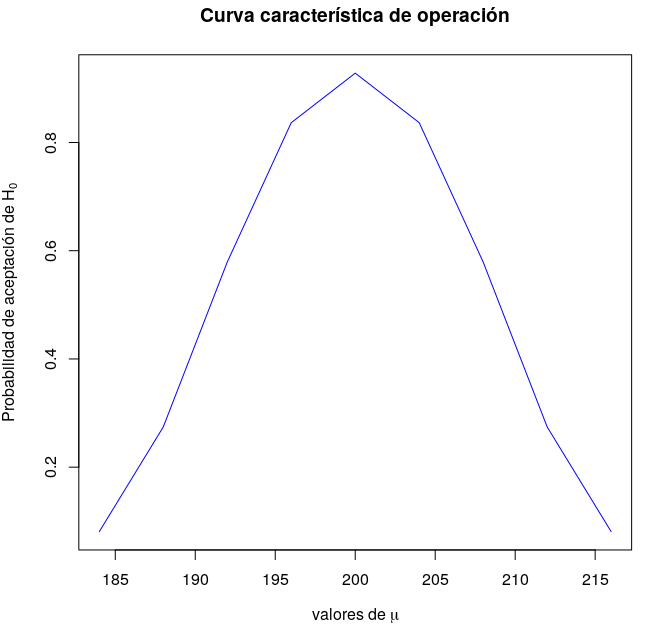
\includegraphics[scale=0.7]{Problema_18_01.png}
 \end{center}
 Aunque una gr\'afica m\'as suave se puede visualizar con los siguientes comandos:
 \begin{verbatim}
> x<-seq(184,216,0.1)
> y<-pnorm(209,mean=x,sd=5)-pnorm(191,mean=x,sd=5)
> plot(x,y,type="l",col="blue",xlab="",ylab="")
> ejexname<-expression(paste("valores de ",mu))
> ejeyname<-expression(paste("Probabilidad de aceptación de ",H[0]))
> title(main="Curva característica de operación",xlab=ejexname,ylab=ejeyname)
 \end{verbatim}
 con lo que se obtiene el siguiente gr\'afico:
 \begin{center}
  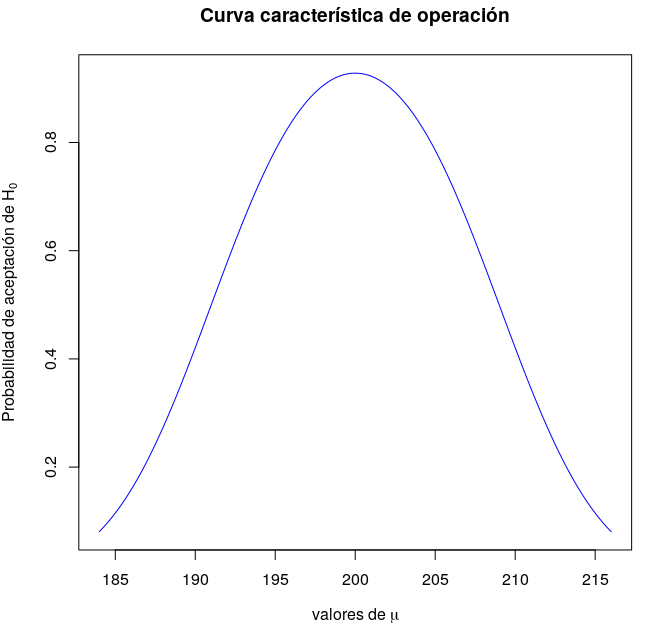
\includegraphics[scale=0.7]{Problema_18_02.png}
 \end{center}
 que es a lo que se quer\'{\i}a llegar.${}_{\blacksquare}$
\end{solucion}

\end{enumerate}

\newpage

\section{Una sola muestra: Pruebas con respecto a una sola media (varianza conocida); Relaci\'on con la estimaci\'on del intervalo de confianza; Una sola muestra: Pruebas sobre una sola media (varianza desconocida); Dos muestras: Pruebas sobre dos medias}

\begin{enumerate}
 \setcounter{enumi}{18}
 \item \begin{enunciado}
 Una empresa de material el\'ectrico fabrica bombillas de luz que tienen una duraci\'on que se distribuye de forma aproximadamente normal con una media de $800$ horas y una desviaci\'on est\'andar de $40$ horas. Pruebe la hip\'otesis de que $\mu = 800$ horas contra la alternativa $\mu \neq 800$ horas, si una muestra aleatoria de $30$ bombillas tiene una duraci\'on promedio de $788$ horas. Utilice un valor $P$ en surespuesta.
\end{enunciado}

\begin{solucion}
 \begin{datos}
  $\phantom{0}$
  \begin{itemize}
   \item $X \sim n(\mu,\sigma)$.
   \item $\overline{X} \sim n\left( \mu, \sigma/\sqrt{n} \right)$.
   \item $\frac{\overline{X}-\mu}{\sigma/\sqrt{n}} \sim n(0,1)$.
   \item $n = 30$.
   \item $\bar{x} = 788$.
   \item $\sigma = 40$.
  \end{itemize}
 \end{datos}

 \begin{hipotesis}
  \begin{eqnarray*}
   H_0: \mu & = & 800 \\
   H_1: \mu & \neq & 800
  \end{eqnarray*}
 \end{hipotesis}

 \begin{estadistico}
  \begin{equation*}
   z = \frac{\bar{x} - \mu_0}{\sigma/\sqrt{n}} = \frac{788-800}{40/\sqrt{30}} = -\frac{12\sqrt{30}}{40} = -\frac{3\sqrt{30}}{10} = -0.3\sqrt{30} \approx -1.643
  \end{equation*}
 \end{estadistico}

 \begin{valorp}
  De la tabla A.3, se tiene que:
  \begin{equation*}
   P(|Z|>|z|) = 2P(Z < -1.64) \approx 2(0.0505) = 0.101 
  \end{equation*}
 \end{valorp}

 \begin{conclusion}
  Dado que, bajo el supuesto de que el tiempo promedio de duraci\'on de las bombillas es de $\mu = 800$ horas, la probabilidad de obtener las mediciones de tiempo de las bombillas con un promedio tan alejado como el obtenido en la muestra es de $P = 0.1$, es decir, que el $10\%$ de todas las posibles muestras est\'an al menos as\'{\i} de alejado del valor hipot\'etico, lo cual no es prueba suficiente para concluir que el tiempo promedio de vida de las bombillas sea distinta a $800$ horas, como dice la empresa.
 \end{conclusion}
 En el c\'odigo registrado en el archivo anexo \texttt{P03\_Prueba\_de\_una\_media\_01.r}, en R, se realiza este procedimiento. El c\'odigo permite modificar los valores iniciales que corresponden a: \texttt{n} para el tama\~no de la muestra; \texttt{mu} para el valor de la media poblacional supuesta en la hip\'otesis nula; \texttt{m} para la media muestral; \texttt{desv} para la desviaci\'on est\'andar poblacional o muestral, seg\'un indique el siguiente par\'ametro; \texttt{pobl} para indicar, con \texttt{TRUE}, si la desviaci\'on est\'andar es poblacional, o con \texttt{FALSE} si es muestral; \texttt{alfa} para el nivel de significancia; \texttt{cola} para indicar si la prueba es de dos colas, con \texttt{'D'}, de cola inferior, con \texttt{'I'}, o de cola superior, con \texttt{'S'}; y, \texttt{val} para indicar, con \texttt{TRUE}, si se tiene el supuesto de que la poblaci\'on sigue una distribuci\'on normal, o con \texttt{FALSE} en otro caso.
 \par 
 El programa espera cuando menos los datos de una muestra, por lo que el valor $P$ siempre se obtiene, independientemente de si se desea una prueba de hip\'otesis fijando la probabilidad del error tipo I o si se realiza una prueba de significancia (aproximaci\'on al valor $P$). Por otro lado, el par\'ametro \texttt{alfa} puede no ser dado, en ese caso se indica con el valor \texttt{NULL}.
 \par 
 La prueba de hip\'otesis puede ser usando el estad\'{\i}stico de la distribuci\'on $Z$ o de la distribuci\'on $t$. Se usar\'a la distribuci\'on $Z$ si la desviaci\'on est\'andar es poblacional o si el tama\~no de muestra es mayor o igual que $30$, en este \'ultimo caso, se usa la desviaci\'on est\'andar muestral como la desviaci\'on poblacional, pues se supone que es buena la aproximaci\'on que se tiene. Si la distribuci\'on es poblacional y la muestra el menor a $30$, entonces se usa la prueba $t$, en otro caso no se realiza ninguna prueba.
 \par 
 El resultado muestra lo siguiente: \texttt{Prueba} para saber si se us\'o el estad\'{\i}stico de distribuci\'on $Z$ o de distribuci\'on $t$; $H_0$ para el valor de la media supuesta; \texttt{n} para el tama\~no de la muestra; \texttt{MediaMuestral} para la media de la muestra; \texttt{desv.est} para la desviaci\'on est\'andar, independientemente de si es la desviaci\'on poblacional o la muestral; \texttt{error.est} para el error est\'andar, que se calcula como $\sigma/\sqrt{n}$, si la desviaci\'on est\'andar es poblacional, o $s/\sqrt{n}$, si la desviaci\'on est\'andar es muestral; \texttt{alpha} para el nivel de significancia dado, el cual muestra por defecto $0.05$ en caso de dar a \texttt{alfa} el valor \texttt{NULL}; \texttt{PValor} para el valor $P$, la probabilidad de haber obtenido una muestra como la que se obtuvo; \texttt{Estadistico} para el valor del estad\'{\i}stico de prueba; \texttt{RegionRechazoZ} o \texttt{RegionRechazoT}, seg\'un el tipo de prueba realizada, que indica en d\'onde se encuentra la regi\'on de rechazo de la distribuci\'on $Z$ o $t$, respectivamente para el valor $\alpha$ dado (aunque sea el valor por defecto); \texttt{RegionRechazoX} para indicar la regi\'on de rechazo en t\'erminos de las unidades del problema original; y, en caso de haber dado un nivel de significancia, \texttt{Resultado} para indicar si se rechaza o no la hip\'otesis nula.
 \par 
 El c\'odigo junto con el resultado se muestra a continuaci\'on:
 \begin{verbatim}
> n<-30
> mu<-800
> m<-788
> desv<-40
> pobl<-TRUE
> alfa<-NULL
> cola<-'D'
> val<-TRUE
> if(!val & n < 30){
+     stop("Se requiere normalidad o muestras grandes")
+ }
> if(!pobl & n >= 30){
+     pobl<-TRUE
+ }
> TestMedia<-function(n,mu,m,desv,alfa=0.05,colas='D',distribucion.z=FALSE){
+     estadistico<-(m-mu)/(desv/sqrt(n))
+     if(n < 2){
+         r<-data.frame(Prueba=NA,
+                       H0=mu,
+                       n=n,
+                       MediaMuestral=m,
+                       desv.est=ifelse(is.na(desv),NA,desv),
+                       error.est=ifelse(is.na(desv),NA,desv/sqrt(n)),
+                       alpha=alfa,
+                       ValorP=NA,
+                       Estadistico=NA,
+                       RegionRechazoZ=NA,
+                       RegionRechazoX=NA)
+     }else{
+         if(distribucion.z){
+             r<-data.frame(Prueba="Z",
+                           H0=mu,
+                           n=n,
+                           MediaMuestral=m,
+                           desv.est=desv,
+                           error.est=desv/sqrt(n),
+                           alpha=alfa)
+             if(colas=='D'){
+                 pvalor<-round(2*pnorm(abs(estadistico),lower.tail=F),7)
+                 criticoz<-round(qnorm(1-alfa/2),7)
+                 criticox<-round(criticoz*desv/sqrt(n),7)
+                 r$PValor<-pvalor
+                 r$Estadistico<-estadistico
+                 r$RegionRechazoZ<-paste("<",-criticoz," y >",criticoz)
+                 r$RegionRechazoX<-paste("<",mu-criticox," y >",mu+criticox)
+             }else{
+                 criticoz<-round(qnorm(1-alfa),7)
+                 criticox<-round(criticoz*desv/sqrt(n),7)
+                 if(colas=='I'){
+                     pvalor<-round(pnorm(estadistico),7)
+                     r$PValor<-pvalor
+                     r$Estadistico<-estadistico
+                     r$RegionRechazoZ<-paste("<",-criticoz)
+                     r$RegionRechazoX<-paste("<",mu-criticox)
+                 }else{
+                     pvalor<-round(pnorm(estadistico,lower.tail=F),7)
+                     r$PValor<-pvalor
+                     r$Estadistico<-estadistico
+                     r$RegionRechazoZ<-paste(">",criticoz)
+                     r$RegionRechazoX<-paste(">",mu+criticox)
+                 }
+             }
+         }else{
+             r<-data.frame(Prueba="t",
+                           H0=mu,
+                           n=n,
+                           MediaMuestral=m,
+                           desv.est=desv,
+                           error.est=desv/sqrt(n),
+                           alpha=alfa)
+             if(colas=='D'){
+                 pvalor=round(2*pt(abs(estadistico),n-1,lower.tail=F),7)
+                 criticot<-round(qt(1-alfa/2,n-1),7)
+                 criticox<-round(criticot*desv/sqrt(n),7)
+                 r$PValor<-pvalor
+                 r$Estadistico<-estadistico
+                 r$RegionRechazoT<-paste("<",-criticot," y >",criticot)
+                 r$RegionRechazoX<-paste("<",mu-criticox," y >",mu+criticox)
+             }else{
+                 criticot<-round(qt(1-alfa,n-1),7)
+                 criticox<-round(criticot*desv/sqrt(n),7)
+                 if(colas=='I'){
+                     pvalor<-round(pt(estadistico,n-1),7)
+                     r$PValor<-pvalor
+                     r$Estadsitico<-estadistico
+                     r$RegionRechazoT<-paste("<",-criticot)
+                     r$RegionRechazoX<-paste("<",mu-criticox)
+                 }else{
+                     pvalor<-round(pt(estadistico,n-1,lower.tail=F),7)
+                     r$PValor<-pvalor
+                     r$Estadistico<-estadistico
+                     r$RegionRechazoT<-paste(">",criticot)
+                     r$RegionRechazoX<-paste(">",mu+criticox)
+                 }
+             }
+         }
+     }
+     return(r)
+ }
> if(is.null(alfa)){
+     Test<-TestMedia(n,mu,m,desv,colas=cola,distribucion.z=pobl)
+ }else{
+     Test<-TestMedia(n,mu,m,desv,alfa,cola,pobl)
+     resultado<-ifelse(Test[,"PValor"]>=alfa,"No se rechaza H0","Se rechaza H0")
+     Test$Resultado<-resultado
+     Test$Resultado[is.na(Test$Resultado)]<-"Pocos datos"
+ }
> Test
  Prueba  H0  n MediaMuestral desv.est error.est alpha    PValor Estadistico
1      Z 800 30           788       40  7.302967  0.05 0.1003482   -1.643168
             RegionRechazoZ                 RegionRechazoX
1 < -1.959964  y > 1.959964 < 785.6864467  y > 814.3135533
 \end{verbatim}
 \vspace{-0.5cm}
 Por lo tanto, se puede observar que, usando la distribuci\'on $Z$, el valor $P$ es aproximadamente $0.1$, el cual indica una falta de capacidad de concluir que el tiempo promedio de las bombilas, en horas, es distinto de $800$, que es a lo que se quer\'{\i}a llegar.${}_{\blacksquare}$
\end{solucion}

 \item \begin{enunciado}
 Una muestra aleatoria de $64$ bolsas de palomitas (rosetas) de ma\'{\i}z con queso chedar pesan, en promedio, $5.23$ onzas con una desviaci\'on est\'andar de $0.24$ onzas. Pruebe la hip\'otesis de que $\mu = 5.5$ onzas contra la hip\'otesis alternativa, $\mu < 5.5$ onzas con un nivel de significancia de $0.05$.
\end{enunciado}

\vspace{0.5cm}

\begin{solucion}
 \begin{datos}
  $\phantom{0}$
  \begin{itemize}
   \item $n = 64$.
   \item $\bar{x} = 5.23$
   \item $s = 0.24$
  \end{itemize}
  Adem\'as, por teorema del l\'{\i}mite central, como $n \geq 30$, se puede aproximar la variable aleatoria de la media muestral a una normal, de lo que se sigue que:
  \begin{itemize}
   \item $\overline{X} \sim n\left( \mu, \sigma/\sqrt{n} \right)$.
   \item $\frac{\overline{X}-\mu}{S/\sqrt{n}} \approx \frac{\overline{X}-\mu}{\sigma/\sqrt{n}} \sim n(0,1)$.
  \end{itemize}
 \end{datos}
 
 \begin{hipotesis}
  \begin{eqnarray*}
   H_0: \mu & = & 5.5 \\
   H_1: \mu & < & 5.5
  \end{eqnarray*}
 \end{hipotesis}

 \begin{significancia}
  $\alpha = 0.05$
 \end{significancia}

 \begin{region}
  De la tabla A.3, se tiene el valor cr\'{\i}tico $z_{\alpha} = z_{0.05} \approx 1.645$, por lo que la regi\'on de rechazo est\'a dado para $z < -1.645$, donde $z = \frac{\bar{x} - \mu}{\sigma/\sqrt{n}}$.
 \end{region}

 \begin{estadistico}
  \begin{equation*}
   z \approx \frac{\bar{x} -\mu}{s/\sqrt{n}} = \frac{5.23-5.5}{0.24/\sqrt{64}} = -\frac{0.27(8)}{0.24} = -\frac{9(8)}{8} = -9
  \end{equation*}
 \end{estadistico}

 \begin{decision}
  Se rechaza $H_0$ a favor de $H_1$.
 \end{decision}

 \begin{conclusion}
  El promedio del peso en las bolsas de palomitas de ma\'{\i}z con queso chedar es menor a $5.5$ onzas.
 \end{conclusion}

 Finalmente, usando el archivo anexo \texttt{P03\_Prueba\_de\_una\_media\_01.r}, con los siguientes cambios:
 \begin{verbatim}
> n<-64
> mu<-5.5
> m<-5.23
> desv<-0.24
> pobl<-FALSE
> alfa<-0.05
> cola<-'I'
> val<-FALSE
 \end{verbatim}
 \vspace{-0.5cm}
 el programa de R lanza el siguiente resultado:
 \begin{verbatim}
  Prueba  H0  n MediaMuestral desv.est error.est alpha PValor Estadistico
1      Z 5.5 64          5.23     0.24      0.03  0.05      0          -9
  RegionRechazoZ RegionRechazoX     Resultado
1   < -1.6448536    < 5.4506544 Se rechaza H0
 \end{verbatim}
 \vspace{-0.5cm}
 El cual coincide con los resultados obtenidos, ofreciendo incluso m\'as informaci\'on, que es a lo que se quer\'{\i}a llegar.${}_{\blacksquare}$
\end{solucion}

 \item \begin{enunciado}
 En un informe de investigaci\'on de Richard H. Weindruch de la Escuela de Medicina de la \texttt{UCLA}, se afirma que los ratones con una vida promedio de 32 meses vivir\'{\i}an hasta alrededor de $40$ meses de edad, cuando 40\% de las calor\'{\i}as en su dieta se reemplacen con vitaminas y prote\'{\i}nas. ¿Hay alguna raz\'on para creer que $\mu < 40$, si $64$ ratones que se sujetan a esa dieta tienen una vida promedio de $38$ meses con una desviaci\'on est\'andar de $5.8$ meses? Utilice un valor $P$ en su conclusi\'on.
\end{enunciado}

\begin{solucion}
 \begin{datos}
  $\phantom{0}$
  \begin{itemize}
   \item $n = 64$.
   \item $\bar{x} = 38$.
   \item $s = 5.8$.
  \end{itemize}
  Adem\'as, por el teorema del l\'{\i}mite central, como $n \geq 30$, se puede aproximar la variable aleatoria de la media muestral a una normal, y usar el estad\'{\i}stico siguiente:
  \begin{itemize}
   \item $\overline{X} \sim n\left( \mu , \sigma/\sqrt{n} \right)$.
   \item $Z = \frac{\overline{X}-\mu}{S/\sqrt{n}} \approx
   \frac{\overline{X} - \mu}{\sigma/\sqrt{n}} \sim n(0,1)$.
  \end{itemize}
 \end{datos}

 \begin{hipotesis}
  \begin{eqnarray*}
   H_0: \mu & = & 40 \\
   H_1: \mu & < & 40
  \end{eqnarray*}
 \end{hipotesis}

 \begin{estadistico}
  \begin{equation*}
   z = \frac{\bar{x}-\mu_0}{\sigma/\sqrt{n}} \approx \frac{\bar{x} - \mu_0}{s/\sqrt{n}} = \frac{38-40}{5.8/\sqrt{64}} = -\frac{2(8)}{5.8} = -\frac{80}{29} \approx -2.75862
  \end{equation*}
 \end{estadistico}

 \begin{valorp}
  De la tabla A.3, se tiene que:
  \begin{equation*}
   P(Z<z) \approx P(Z < -2.76) \approx 0.0029
  \end{equation*}
 \end{valorp}

 \begin{conclusion}
  Dado que el valor $P$ es muy peque\~no,
  tanto que \'unicamente hay un aproximado $0.3\%$ de las muestras
  que pueden dar resultados similares,
  es evidencia suficiente para rechazar la afirmaci\'on de la escuela
  de Medicina de la UCLA y concluir que la vida promedio de los ratones
  con una vida promedio de 32 meses que sigue una dieta
  en el que se reemplaza el 40\% de calor\'{\i}as con vitaminas
  y prote\'{\i}nas es significativamente menor a los 40 meses.
 \end{conclusion}
 Finalmente, usando el archivo anexo \texttt{P03\_Prueba\_de\_una\_media\_01.r}, con los siguientes cambios:
 \begin{verbatim}
> n<-64
> mu<-40
> m<-38
> desv<-5.8
> pobl<-FALSE
> alfa<-NULL
> cola<-'I'
> val<-FALSE
 \end{verbatim}
 \vspace{-0.5cm}
 el programa de R lanza el siguiente resultado:
 \begin{verbatim}
  Prueba H0  n MediaMuestral desv.est error.est alpha    PValor Estadistico
1      Z 40 64            38      5.8     0.725  0.05 0.0029023   -2.758621
  RegionRechazoZ RegionRechazoX
1   < -1.6448536   < 38.8074811
 \end{verbatim}
 \vspace{-0.5cm}
 El cual coincide con los resultados obtenidos, que es a lo que se quer\'{\i}a llegar.${}_{\blacksquare}$
\end{solucion}

 \item \begin{enunciado}
 La estatura promedio de mujeres en el grupo de primer a\~no de cierta universidad es de $162.5$ cent\'{\i}metros con una desviaci\'on est\'andar de $6.9$ cent\'{\i}metros. ¿Hay alguna raz\'on para creer que hay un cambio en la estatura promedio, si una muestra aleatoria de $50$ mujeres en el grupo actual de primer a\~no tiene una altura promedio de $165.2$ cent\'{\i}metros? Utilice un valor $P$ en su conclusi\'on. Suponga que la desviaci\'on est\'andar permanece constante.
\end{enunciado}

\begin{solucion}
 \begin{datos}
  $\phantom{0}$
  \begin{itemize}
   \item $n = 50$.
   \item $\bar{x} = 162.5$.
   \item $\sigma = 6.9$.
  \end{itemize}
  Adem\'as, por el teorema del l\'{\i}mite central, como $n \geq 30$, se puede aproximar la variable aleatoria de la media muestral a una normal, y usar el estad\'{\i}stico siguiente:
  \begin{itemize}
   \item $\overline{X} \sim n\left( \mu , \sigma/\sqrt{n} \right)$.
   \item $Z = \frac{\overline{X} - \mu}{\sigma/\sqrt{n}}
   \sim n(0,1)$.
  \end{itemize}
 \end{datos}

 \begin{hipotesis}
  \begin{eqnarray*}
   H_0: \mu & = & 162.5 \\
   H_1: \mu & \neq & 162.5
  \end{eqnarray*}
 \end{hipotesis}

 \begin{estadistico}
  \begin{equation*}
   z = \frac{\bar{x} - \mu_0}{\sigma/\sqrt{n}} = \frac{165.2-162.5}{6.9/\sqrt{50}} = \frac{2.7(5)\sqrt{2}}{6.9} = \frac{135\sqrt{2}}{69} = \frac{45\sqrt{2}}{23} \approx 2.766939578556
  \end{equation*}
 \end{estadistico}

 \begin{valorp}
  De la tabla A.3, se tiene que:
  \begin{equation*}
   P(|Z| > |z|) \approx 2P(Z < -2.77) \approx 2(0.0028) = 0.0056
  \end{equation*}
 \end{valorp}

 \begin{conclusion}
  El valor $P$ es peque\~no, lo cual es evidencia suficiente para rechazar la hip\'otesis nula de que la estatura promedio de mujeres de primer a\~no en la universidad se mantiene en $162.5\,$cm y concluir a favor de que ha cambiado la estatura de estas mujeres.
 \end{conclusion}
 Finalmente, usando el archivo anexo \texttt{P03\_Prueba\_de\_una\_media\_01.r}, con los siguientes cambios:
 \begin{verbatim}
> n<-50
> mu<-162.5
> m<-165.2
> desv<-6.9
> pobl<-TRUE
> alfa<-NULL
> cola<-'D'
> val<-FALSE
 \end{verbatim}
 \vspace{-0.5cm}
 el programa de R lanza el siguiente resultado:
 \begin{verbatim}
  Prueba    H0  n MediaMuestral desv.est error.est alpha    PValor Estadistico
1      Z 162.5 50         165.2      6.9 0.9758074  0.05 0.0056585     2.76694
             RegionRechazoZ                 RegionRechazoX
1 < -1.959964  y > 1.959964 < 160.5874527  y > 164.4125473
 \end{verbatim}
 \vspace{-0.5cm}
 El cual coincide con los resultados obtenidos, que es a lo que se quer\'{\i}a llegar.${}_{\blacksquare}$
\end{solucion}

 \item \begin{enunciado}
 Se afirma que un autom\'ovil se maneja en promedio m\'as de $20,000$ kil\'ometros por a\~no. Para probar tal afirmaci\'on, se pide a una muestra de $100$ propietarios de autom\'oviles que lleven un registro de los kil\'ometros que recorran. ¿Estar\'{\i}a usted de acuerdo con esta afirmaci\'on, si la muestra aleatoria mostr\'o un promedio de $23,500$ kil\'ometros y una desviaci\'on est\'andar de $3900$ kil\'ometros? Utilice un valor $P$ en su conclusi\'on.
\end{enunciado}

\begin{solucion}
 \begin{datos}
  $\phantom{0}$
  \begin{itemize}
   \item $n=100$.
   \item $\bar{x} = 23\,500$.
   \item $s = 3\,900$.
  \end{itemize}
  Adem\'as, por el teorema del l\'{\i}mite central, como $n \geq 30$, se puede aproximar la variable aleatoria de la media muestral a una normal, y usar el estad\'{\i}stico siguiente:
  \begin{itemize}
   \item $\overline{X} \sim n\left( \mu , \sigma/\sqrt{n} \right)$.
   \item $Z = \frac{\overline{X}-\mu}{S/\sqrt{n}} \approx
   \frac{\overline{X} - \mu}{\sigma/\sqrt{n}} \sim n(0,1)$.
  \end{itemize}
 \end{datos}

 \begin{hipotesis}
  \begin{eqnarray*}
   H_0: \mu & \leq & 20\,000 \\
   H_1: \mu & > & 20\,000
  \end{eqnarray*}
 \end{hipotesis}

 \begin{estadistico}
  \begin{equation*}
   z = \frac{\bar{x} - \mu_0}{\sigma/\sqrt{n}} \approx \frac{\bar{x} - \mu_0}{s/\sqrt{n}} = \frac{23\,500 - 20\,000}{3\,900/\sqrt{100}} = \frac{350}{39} = 8.\overline{974358}
  \end{equation*}
 \end{estadistico}

 \begin{valorp}
  De la tabla A.3, se tiene que:
  \begin{equation*}
   P\left( Z > z \right) \approx P(Z > 8.97) = P(Z < -8.97) \approx 0
  \end{equation*}
 \end{valorp}

 \begin{conclusion}
  Por lo tanto, como el valor $P < 0.0001$, entonces se tiene evidencia suficiente para concluir que el autom\'ovil se maneja en promedio m\'as de $20\,000$ kil\'ometros, como bien se afirma.
 \end{conclusion}
 Finalmente, usando el archivo anexo \texttt{P03\_Prueba\_de\_una\_media\_01.r}, con los siguientes cambios:
 \begin{verbatim}
> n<-100
> mu<-20000
> m<-23500
> desv<-3900
> pobl<-FALSE
> alfa<-NULL
> cola<-'S'
> val<-FALSE
 \end{verbatim}
 \vspace{-0.5cm}
 el programa de R lanza el siguiente resultado:
 \begin{verbatim}
  Prueba    H0   n MediaMuestral desv.est error.est alpha PValor Estadistico
1      Z 20000 100         23500     3900       390  0.05      0    8.974359
  RegionRechazoZ RegionRechazoX
1    > 1.6448536 > 20641.492904
 \end{verbatim}
 \vspace{-0.5cm}
 El cual coincide con los resultados obtenidos, que es a lo que se quer\'{\i}a llegar.${}_{\blacksquare}$
\end{solucion}

 \item \begin{enunciado}
 En el bolet\'{\i}n de la Asociaci\'on Estadounidense del Coraz\'on, \textit{Hypertension}, investigadores reportan que los individuos que practican la meditaci\'on trascendental (\texttt{MT}) bajan su presi\'on sangu\'{\i}nea de forma significativa. Si una muestra aleatoria de $225$ hombres practicantes de \texttt{MT} meditan $8.5$ horas a la semana, con una desviaci\'on est\'andar de $2.25$ horas, ¿esto sugiere que, en promedio, los hombres que utilizan la \texttt{MT} meditan m\'as de $8$ horas a la semana? Cite un valor $P$ en su conclusi\'on.
\end{enunciado}

\begin{solucion}
 \begin{datos}
  $\phantom{0}$
  \begin{itemize}
   \item $n = 225$.
   \item $\bar{x} = 8.5$.
   \item $s = 2.25$.
  \end{itemize}
  Adem\'as, por el teorema del l\'{\i}mite central, como $n \geq 30$, se puede aproximar la variable aleatoria de la media muestral a una normal, y usar el estad\'{\i}stico siguiente:
  \begin{itemize}
   \item $\overline{X} \sim n\left( \mu , \sigma/\sqrt{n} \right)$.
   \item $Z = \frac{\overline{X}-\mu}{S/\sqrt{n}} \approx
   \frac{\overline{X} - \mu}{\sigma/\sqrt{n}} \sim n(0,1)$.
  \end{itemize}
 \end{datos}

 \begin{hipotesis}
  \begin{eqnarray*}
   H_0: \mu & \leq & 8 \\
   H_1: \mu & > & 8
  \end{eqnarray*}
 \end{hipotesis}

 \begin{estadistico}
  \begin{equation*}
   z = \frac{\bar{x} - \mu_0}{\sigma/\sqrt{n}} \approx \frac{\bar{x} - \mu_0}{s/\sqrt{n}} = \frac{8.5-8}{2.25/\sqrt{225}} = \frac{0.5(15)}{2.25} = \frac{150}{45} = \frac{10}{3} = 3.\overline{3}
  \end{equation*}
 \end{estadistico}

 \begin{valorp}
  De la tabla A.3 se tiene que:
  \begin{equation*}
   P(Z > z) \approx P(Z > 3.33) = P(Z < -3.33) \approx 0.0004
  \end{equation*}
 \end{valorp}

 \begin{conclusion}
  Por lo tanto, como el valor $P$ es muy peque\~no, entonces se tiene evidencia suficiente para concluir que los hombres que utilizan la MT meditan m\'as de $8\,$hrs a la semana.
 \end{conclusion}
 Finalmente, usando el archivo anexo \texttt{P03\_Prueba\_de\_una\_media\_01.r}, con los siguientes cambios:
 \begin{verbatim}
> n<-225
> mu<-8
> m<-8.5
> desv<-2.25
> pobl<-FALSE
> alfa<-NULL
> cola<-'S'
> val<-FALSE
 \end{verbatim}
 \vspace{-0.5cm}
 el programa de R lanza el siguiente resultado:
 \begin{verbatim}
  Prueba H0   n MediaMuestral desv.est error.est alpha    PValor Estadistico
1      Z  8 225           8.5     2.25      0.15  0.05 0.0004291    3.333333
  RegionRechazoZ RegionRechazoX
1    > 1.6448536     > 8.246728
 \end{verbatim}
 \vspace{-0.5cm}
 El cual coincide con los resultados obtenidos, que es a lo que se quer\'{\i}a llegar.${}_{\blacksquare}$
\end{solucion}

 \item \begin{enunciado}
 Considere el ejercicio 9.12. Calcule un intervalo de predicci\'on de $95\%$ para el contenido de az\'ucar de la siguiente porci\'on sencilla del cereal Alpha-Bits.
\end{enunciado}

\begin{solucion}
 Usando la notaci\'on y datos como se explic\'o en la soluci\'on del ejercicio 9.12 pero ahora con $\alpha$ representando el valor para el cual hay $(1-\alpha)100\%$ de seguridad en el intervalo de predicci\'on, se tiene lo siguiente:
 \begin{itemize}
  \item $X\sim n(\mu,\sigma)$.
  \item $\mu$ desconocida.
  \item $\sigma$ desconocida.
  \item $n = 20$ porciones.
  \item $\bar{x}=11.3\,$g.
  \item $s=2.45\,$g.
  \item $\alpha=0.05$.
  \item $t_{\alpha/2,n-1} = t_{0.025,19} = 2.093$, seg\'un la Tabla A.4 del libro, y $t_{0.025,19} = 2.093024$, usando el software estad\'{\i}stico R.
 \end{itemize}
 Como se est\'a buscando un intervalo de predicci\'on para una muestra peque\~na que proviene de una poblaci\'on normal con varianza desconocida, entonces se usar\'a la siguiente formulaci\'on:
 \begin{equation*}
  \bar{x} - t_{\alpha/2,n-1} s \sqrt{1 + 1/n} < x_0 < \bar{x} + t_{\alpha/2,n-1} s \sqrt{1 + 1/n}
 \end{equation*}
 Por lo tanto, con los datos obtenidos y el valor $t_{\alpha/2,n-1}$ del libro, se tienen los c\'alculo de los l\'{\i}mites del intervalo de predicci\'on como siguen:
 \begin{equation*}
  \bar{x} \pm t_{\alpha/2,n-1} s \sqrt{1 + 1/n} = 11.3 \pm (2.093)(2.45)\sqrt{1+\frac{1}{20}} = 11.3 \pm 5.12785 \frac{\sqrt{21}}{2\sqrt{5}} = 11.3\pm 0.512785\sqrt{105}
 \end{equation*}
 Por lo tanto, el intervalo de predicci\'on de $95\%$ para el contenido de az\'ucar en la siguiente porci\'on sencilla del cereal Alpha-Bits es de:
 \begin{equation*}
  6.0455173514774 < x_0 < 16.55448264852
 \end{equation*}
 que redondeado al segundo decimal se reduce a que el intervalo es $(6.05, 16.55)$. Por otro lado, el c\'alculo del intervalo de predicci\'on usando el valor $t_{\alpha/2, n-1}$ obtenido en R se puede realizar con los siguientes comandos. Los c\'odigos escritos se encuentran registrados en un script en el archivo anexo \texttt{P08\_Intervalo\_de\_prediccion\_1.r}. El resultado mostrado al final presenta el l\'{\i}mite inferior, la media muestral y el l\'{\i}mite superior, en ese orden, que se encuentra almacenado en la variable \texttt{IT}. La variable \texttt{val} indica si se conoce o no la varianza poblacional, de todos modos se considera \texttt{TRUE} si el tama\~no de muestra es grande, es decir, se aproximar\'a la desviaci\'on poblacional usando la desviaci\'on muestral si la muestra es mayor o igual a $30$.
 
 \begin{verbatim}
>n<-20
>m<-11.3
>desv<-2.45
>alfa<-0.05
>val<-FALSE
>if (n >= 30)
>{
>    val<-TRUE
>}
>k<-ifelse(val,round(qnorm(1-alfa/2),7),round(qt(1-alfa/2,n-1),7))
>LL<-m-k*desv*sqrt(1+1/n)
>LU<-m+k*desv*sqrt(1+1/n)
>IP<-data.frame(LL,m,LU)
>names(IP)[names(IP) == "LL"]<-"LimInf"
>names(IP)[names(IP) == "m"]<-"Media"
>names(IP)[names(IP) == "LU"]<-"LimSup"
>IP
    LimInf Media   LimSup
1 6.045457  11.3 16.55454
 \end{verbatim}
 que es a lo que se quer\'{\i}a llegar.${}_{\blacksquare}$
\end{solucion}

 \item \begin{enunciado}
 De acuerdo con un estudio diet\'etico una ingesta alta de sodio se puede relacionar con \'ulceras, c\'ancer estomacal y migra\~na. El requerimiento humano de sal es de tan s\'olo $220$ miligramos diarios, el cual se rebasa en la mayor\'{\i}a de las porciones individuales de cereales listos para comerse. Si una muestra aleatoria de $20$ porciones similares de cierto cereal tiene un contenido medio de $244$ miligramos de sodio y una desviaci\'on est\'andar de $24.5$ miligramos, ¿esto sugiere, en el nivel de significancia de $0.05$, que el contenido promedio de sodio para porciones individuales de tal cereal es mayor que $220$ miligramos? Suponga que la distribuci\'on de contenidos de sodio es normal.
\end{enunciado}

\begin{solucion}
 \begin{datos}
  $\phantom{0}$
  \begin{itemize}
   \item $X \sim n(\mu, \sigma)$.
   \item $n = 20$.
   \item $\bar{x} = 244$.
   \item $s = 24.5$.
  \end{itemize}
  Por la suposici\'on de normalidad en la distribuci\'on
  poblacional, se tiene la distribuci\'on siguiente:
  \begin{itemize}
   \item $\displaystyle{\frac{\overline{X} - \mu}{S/\sqrt{n}}  \sim t(v) }$.
   \item $v = n-1 = 19$.
  \end{itemize}
 \end{datos}

 \begin{hipotesis}
  \begin{eqnarray*}
   H_0: \mu & = & 220 \\
   H_1: \mu & > & 220
  \end{eqnarray*}
 \end{hipotesis}

 \begin{significancia}
  $a = 0.05$.
 \end{significancia}

 \begin{region}
  De la tabla A.4, se tiene el valor cr\'{\i}tico $t_{\alpha,n-1} = t_{0.05,19} = 1.729$, por lo que la regi\'on de rechazo est\'a dado para $t > 1.729$, donde $t = \frac{\bar{x} - \mu_0}{s/\sqrt{n}}$.
 \end{region}

 \begin{estadistico}
  \begin{equation*}
   t = \frac{\bar{x}-\mu_0}{s/\sqrt{n}} = \frac{244-220}{24.5/\sqrt{20}} = \frac{24(2)\left(2\sqrt{5}\right)}{49} = \frac{96\sqrt{5}}{49} \approx 4.380867874
  \end{equation*}
 \end{estadistico}

 \begin{decision}
  Se rechaza $H_0$ a favor de $H_1$.
 \end{decision}

 \begin{conclusion}
  El contenido promedio de sodio para porciones individuales del cereal es significativamente mayor a los $220$ miligramos.
 \end{conclusion}

 Finalmente, usando el archivo anexo \texttt{P03\_Prueba\_de\_una\_media\_01.r}, con los siguientes cambios:
 \vspace{-0.3cm}
 \begin{verbatim}
> n<-20
> mu<-220
> m<-244
> desv<-24.5
> pobl<-FALSE
> alfa<-0.05
> cola<-'S'
> val<-TRUE
 \end{verbatim}
 \vspace{-0.8cm}
 el programa de R lanza el siguiente resultado:
 \vspace{-0.3cm}
 \begin{verbatim}
  Prueba  H0  n MediaMuestral desv.est error.est alpha    PValor Estadistico
1      t 220 20           244     24.5  5.478367  0.05 0.0001607    4.380868
  RegionRechazoT RegionRechazoX     Resultado
1    > 1.7291328  > 229.4728233 Se rechaza H0
 \end{verbatim}
 \vspace{-0.8cm}
 El cual coincide con los resultados obtenidos, que es a lo que se quer\'{\i}a llegar.${}_{\blacksquare}$
\end{solucion}

 \item \begin{enunciado}
 Un estudio de la Universidad de Colorado en Boulder muestra que correr aumenta el porcentaje de la tasa metab\'olica de descanso (\texttt{TMD}) en mujeres ancianas. La \texttt{TMD} promedio de $30$ ancianas corredoras fue $34.0\%$ m\'as alta que la \texttt{TMD} promedio de $30$ ancianas sedentarias, en tanto que las desviaciones est\'andar reportadas fueron de $10.5$ y $10.2\%$, respectivamente. ¿Hay un aumento significativo en la \texttt{TMD} de las corredoras con respecto a las sedentarias? Suponga que las poblaciones se distribuyen de forma aproximadamente normal con varianzas iguales. Utilice un valor $P$ en sus conclusiones.
\end{enunciado}

\begin{solucion}
 \begin{datos}
  $\phantom{0}$
  \begin{itemize}
   \item $X_i \sim n\left( \mu_i, \sigma_i \right)$, para cada $i \in \{ 1, 2 \}$.
   \item $n_1 = 30$ y $n_2 = 30$.
   \item $\bar{x}_1 - \bar{x}_2 = 34$.
   \item $s_1 = 10.5$ y $s_2 = 10.2$.
   \item $\sigma_1^2 = \sigma_2^2$.
  \end{itemize}
  Ya que $n_1, n_2 \geq 30$,
  como resultado del teorema del teorema del l\'{\i}mite central
  se obtiene adem\'as que los siguientes estadísticos se aproximan
  a las distribuciones indicadas:
  \begin{itemize}
   \item $\overline{X}_i \sim n\left( \mu_i, \sigma_i/n \right)$,
   para cada $i \in \{ 1, 2 \}$.
   \item $Z = \frac{\left( \overline{X}_1 - \overline{X}_2 \right) - d_0}{\sqrt{S_1^2/n_1 + S_2^2/n_2}} \approx
   \frac{\left( \overline{X}_1 - \overline{X}_2 \right) - d_0}{\sqrt{\sigma_1^2/n_1 + \sigma_2^2/n_2}}
   \sim n\left( 0, 1 \right)$.
  \end{itemize}
  A\'un as\'{\i}, si no se contara con dichos resultados,
  por las suposiciones de normalidad en la distribuciones
  poblacionales y que las varianzas son iguales, se sabe
  que el siguiente estad\'{\i}stico,
  que se aproxima a la distribuci\'on mostrada
  con el respectivo par\'ametro que se indica,
  se puede usar en vez del anterior.
  \begin{itemize}
   \item $T = 
   \frac{\left( \overline{X}_1 - \overline{X}_2 \right) - d_0}{S_p\sqrt{1/n_1 + 1/n_2}} \sim t(v)$.
   \item $v = n_1 + n_2 - 2 = 58$.
  \end{itemize}
 \end{datos}

 \begin{hipotesis}
  \begin{eqnarray*}
   H_0: \mu_1 - \mu_2 & = & 0 \\
   H_1: \mu_1 - \mu_2 & > & 0
  \end{eqnarray*}
 \end{hipotesis}

 \begin{estadistico}
  Usando el estad\'{\i}stico obtenido con el teorema
  del l\'{\i}mite central, se calcula que:
  \begin{eqnarray*}
   z & = & \frac{\left( \bar{x}_1 - \bar{x}_2 \right) - \left( \mu_1 - \mu_2 \right)}{\sqrt{s_1^2/n_1 + s_2^2/n_2}}
   \approx \frac{34-0}{\sqrt{10.5^2/30 + 10.2^2/30}}
   = \frac{34\sqrt{30}}{\sqrt{110.25+104.04}}
   = \frac{34(10)\sqrt{30}}{\sqrt{21\,429}} \\
   & = & \frac{340\sqrt{10}}{\sqrt{7\,143}}
   = \frac{340\sqrt{71\,430}}{7143} \approx 12.7215079
  \end{eqnarray*}
  A\'un as\'{\i}, el valor con el otro estad\'{\i}stico
  se obtiene calculando primero lo siguiente:
  \begin{eqnarray*}
   s_p^2 & = &
   \frac{
   s_1^2 \left( n_1 - 1 \right) + s_2^2\left( n_2 - 1 \right)
   }{
   n_1 + n_2 - 2
   }
   = \frac{10.5^2(30-1) + 10.2(30-1)}{30+30-2}
   = \frac{\cancel{29}(110.25 + 104.04)}{\cancelto{2}{58}} \\
   & = & \frac{21\,429}{200}
   = 107.145
  \end{eqnarray*}
  entonces
  \begin{equation*}
   s_p = \sqrt{s_p^2} = \sqrt{\frac{21\,429}{200}}
   = \frac{3\sqrt{2\,381}\sqrt{2}}{20}
   = \frac{3\sqrt{4\,762}}{20}
   \approx 10.351086899451670625994809052
  \end{equation*}
  y, por lo tanto,
  \begin{eqnarray*}
   t & = & 
   \frac{
   \left( \bar{x}_1 - \bar{x}_2 \right) - d_0
   }{
   s_p\sqrt{1/n_1 + 1/n_2}
   }
   = \frac{34-0}{\frac{3\sqrt{4\,762}}{20}\sqrt{\frac{1}{30}+\frac{1}{30}}}
   = \frac{34(20)}{3\sqrt{\frac{4\,762}{15}}}
   = \frac{680\sqrt{15}\sqrt{4\,762}}{3(4\,762)} \\
   & = & \frac{340\sqrt{71\,430}}{7\,143}
   \approx 12.7215079
  \end{eqnarray*}
 \end{estadistico}

 \begin{valorp}
  De la tabla A.3 se tiene que:
  \begin{equation*}
   P(Z > z) \approx P(Z > 12.72) \approx 0 
  \end{equation*}
  Por otro lado, usando el estad\'{\i}stico $T$, se tiene que:
  \begin{equation*}
   P(T > t) \approx P(T > 12.721507900588463860701)
  \end{equation*}
  Pero usando la tabla A.4 con 58 grados de libertad,
  se buscar\'{\i}a interpolar con los valores m\'as cercanos;
  sin embargo, estos est\'an muy por afuera del rango de la tabla,
  a saber, con $60$ grados de libertad,
  el valor m\'as grande es $3.460$
  y $P(T > 3.460) = 0.0005$,
  mientras que con $40$ grados de libertad,
  el valor m\'as grande es $3.551$
  y $P(T > 3.551) = 0.0005$, por lo que se puede asegurar que
  \begin{equation*}
   P(T > t) \approx P(T > 12.721507900588463860701) < 0.0005
  \end{equation*}
 \end{valorp}

 \begin{conclusion}
  Por lo tanto, como el valor $P$ es muy peque\~no, entonces se tiene evidencia suficiente para concluir que las mujeres ancianas corredoras tienen un porcentaje en la tasa metab\'olica de descanso mayor que las mujeres ancianas sedentarias.
 \end{conclusion}

 En el c\'odigo registrado en el archivo anexo
 \texttt{P05\_Prueba\_de\_dos\_medias\_01.r}, en R,
 se realiza este procedimiento.
 El c\'odigo permite modificar los valores iniciales
 que corresponden a:
 \texttt{n1} y \texttt{n2} para el tama\~no de las muestras;
 \texttt{mu} para el valor de la diferencia de las medias
 poblacionales supuesta en la hip\'otesis nula;
 \texttt{m1} y \texttt{m2} para las medias muestrales o,
 en su defecto, \texttt{m} para la diferencia de estas
 si se da el dato directamente;
 \texttt{sigma1} y \texttt{sigma2} para las desviaciones est\'andar
 poblacionales, si se indican,
 o, en su defecto, \texttt{s1} y \texttt{s2}
 para las desviaciones est\'andar muestrales;
 \texttt{desv.iguales} indica,
 en caso de que se desconozcan las desviaciones est\'andar
 o varianzas poblacionales, si se est\'an suponiendo iguales,
 con el valor \texttt{TRUE}, o diferentes, con \texttt{FALSE};
 \texttt{alfa} para el nivel de significancia;
 \texttt{cola} para indicar si la prueba es de dos colas,
 con \texttt{'D'}, de cola inferior, con \texttt{'I'},
 o de cola superior, con \texttt{'S'};
 adicionalmente, la rutina puede realizar pruebas pareadas
 con \texttt{par} al darle el valor \texttt{TRUE},
 que por defecto aparece como \texttt{FALSE}.
 Esta \'ultima prueba puede necesitar del valor de la desviaci\'on
 est\'andar de la diferencia de los datos pareados,
 para lo que se usa el valor de \texttt{sD}.
 \par 
 El programa espera al menos los datos correspondientes
 a la muestra:
 el tama\~no de ambas muestras;
 la diferencia de las medias muestrales,
 que en caso de dar los valores individuales,
 la rutina calcula la diferencia previo a la funci\'on principal;
 las desviaciones est\'andar, ya sean poblacionales
 o muestrales, o en caso de ser muestras pareadas,
 la desviaci\'on estandar muestral de la diferencia;
 y el tipo de prueba (cola izquierda o derecha, o dos colas);
 y, en caso de ser muestras peque\~nas,
 la suposici\'on sobre si son o no iguales
 las desviaciones est\'andar poblacionales.
 Por lo tanto, el valor $P$ siempre se obtiene,
 independientemente de si se desea una prueba de hip\'otesis
 fijando la probabilidad del error tipo I
 o si se realiza una prueba de significancia
 (aproximaci\'on al valor $P$).
 Los valores no dados, ya sea por redundancia o por ser opcionales,
 se indican con el valor \texttt{NULL},
 excepto \texttt{par} que por defecto tiene el valor \texttt{FALSE}.
 \par 
 La prueba de hip\'otesis usar\'a alg\'un estad\'{\i}stico,
 seg\'un corresponda, que tiene distribuci\'on $Z$ o $t$.
 Se considerar\'a la de distribuci\'on $Z$ si se dan
 las desviaciones est\'andar poblacionales o,
 como estimadores de \'estas,
 las desviaciones est\'andar muestrales.
 Esto \'ultimo ocurrir\'a \'unicamente
 si los tama\~nos de cada muestra son mayores o iguales que $30$.
 Si no se dan las desviaciones est\'andar poblacionales
 y las muestras son peque\~nas,
 se usar\'a el estad\'{\i}stico con distribuci\'on $t$
 y, en dado caso, una condici\'on necesaria y que se va a suponer
 es que las distribuciones poblacionales son aproximadamente
 normales.
 Adem\'as, como ya se mencion\'o, se considerar\'a la prueba
 de muestras pareadas.
 \par
 Independientemente del tipo de prueba,
 el resultado muestra lo siguiente:
 \texttt{Prueba} para saber si se us\'o un estad\'{\i}stico
 con distribuci\'on $Z$ o con distribuci\'on $t$;
 \texttt{H0} para el valor propuesto de la diferencia
 de las medias poblacionales;
 \texttt{n1} y \texttt{n2} para el tama\~no de cada muestra;
 \texttt{DifMedias} o \texttt{MediaPareada}
 para la diferencia de las medias muestrales,
 seg\'un son muestras independientes o pareadas;
 \texttt{desv.est1} y \texttt{desv.est2} para las desviaciones
 est\'andar, ya sea poblacional o muestral seg\'un sea el caso,
 que, en el caso de las muestras pareadas, se sustituye
 por \texttt{desv.par};
 \texttt{error.est} para el error est\'andar,
 cuya f\'ormula var\'{\i}a entre un estad\'{\i}stico y otro,
 pero, independientemente,
 cuando este error divide a
 $\left(\bar{x}_1 - \bar{x}_2\right) - d_0$
 se obtiene el estad\'{\i}stico,
 y representa la estimaci\'on de la desviaci\'on est\'andar
 de $\overline{X}_1 - \overline{X}_2$;
 \texttt{alpha} para el nivel de significancia dado,
 el cual muestra por defecto $0.05$
 en caso de asignar \texttt{NULL} a \texttt{alfa};
 \texttt{PValor} para el valor $P$,
 la probabilidad de haber obtenido una muestra como se obtuvo,
 suponiendo que la hip\'otesis nula sea cierta;
 \texttt{Estadistico} para el valor resultante
 del estad\'{\i}stico de prueba;
 \texttt{RegionRechazoZ} o \texttt{RegionRechazoT},
 seg\'un el tipo de prueba realizada,
 que indica en d\'onde se encuentra la regi\'on de rechazo para
 los valores obtenidos por el estad\'{\i}stico de prueba,
 seg\'un el valor de $\alpha$ (posiblemente el dado por defecto);
 \texttt{RegionRechazoX} para indicar la regi\'on de rechazo,
 en t\'erminudos de las unidades originales del problema,
 para el valor de \texttt{m},
 la diferencia de las medias muestrales.
 \par 
 Adem\'as, seg\'un el tipo de prueba,
 pueden darse los siguientes valores:
 \texttt{Resultado} para indicar si se rechaza o no la hip\'otesis
 nula, que aparece cuando se asigna un valor a \texttt{alfa}, y se encuentra siempre al final de los resultados;
 \texttt{var.pobl} aparece cuando se realiza una prueba $t$, 
 no se conocen las desviaciones est\'andar poblacionales,
 y este valor indica si se est\'an suponiendo iguales o distintos,
 aparece despu\'es de \texttt{Prueba};
 \texttt{est.sp} aparece cuando se realiza una prueba $t$
 y se est\'a suponiendo varianzas iguales,
 este valor indica el resultado
 de calcular $s_p$, el estimador de la desviaci\'on est\'andar
 poblacional com\'un $\sigma$ de las distribuciones poblacionales
 de las que se est\'an obteniendo las muestras,
 aparece despu\'es de las desviaciones est\'andar muestrales;
 \texttt{grados.libertad} aparece cuando se realiza una prueba $t$,
 indica los grados de libertad
 que es el par\'ametro de la distribuci\'on $t$
 del estad\'{\i}stico,
 entre el valor del error est\'andar y $\alpha$;
 \texttt{Tipo} aparece \'unicamente cuando se trata de una prueba
 con muestras dependientes, es decir muestras pareadas,
 indicando el texto: \textit{Muestras pareadas}.
 \par 
 El c\'odigo junto con el resultado se muestra a continuaci\'on:
 \begin{verbatim}
> n1<-30
> n2<-30
> mu<-0
> m1<-NULL
> m2<-NULL
> m<-34
> sigma1<-NULL
> sigma2<-NULL
> s1<-10.5
> s2<-10.2
> sD<-NULL
> desv.iguales<-TRUE
> alfa<-NULL
> cola<-'S'
> par<-FALSE
> if(is.null(m)) m<-m1-m2
> if(n1>=30 & n2>=30){
+    if(is.null(sigma1)) sigma1<-s1
+    if(is.null(sigma2)) sigma2<-s2
+ }
> if(par & n1 != n2){
+    stop("Las muestras pareadas deben tener el mismo tamaño.")
+ }
> TestMedia<-function(n1,n2,mu,m,desv1,desv2,sD=NULL,alfa=0.05,colas='D',
+                     conocidas=FALSE,iguales=FALSE,pareadas=FALSE){
+   if(n1 < 2 | n2 < 2 | par & is.null(sD)){
+     if(is.null(sD)){
+        error<-ifelse(is.na(desv1)|is.na(desv2),
+                      NA,sqrt(desv1^2/n1+desv2^2/n2))
+     }else{
+        error<-sD
+     }
+     r<-data.frame(Prueba=NA, H0=mu,
+                   n1=n1, n2=n2,
+                   DifMedias=m,
+                   desv.est1=ifelse(is.na(desv1),NA,desv1),
+                   desv.est2=ifelse(is.na(desv2),NA,desv2),
+                   error.est=error,
+                   alpha=alfa,
+                   PValor=NA,
+                   Estadistico=NA,
+                   RegionRechazoZ=NA,
+                   RegionRechazoX=NA)
+   }
+   estadistico<-m-mu
+   if(!pareadas){
+     if(conocidas){
+       desv<-sqrt(desv1^2/n1+desv2^2/n2)
+       estadistico<-estadistico/desv
+       r<-data.frame(Prueba="Z",H0=mu,
+                     n1=n1, n2=n2,
+                     DifMedias=m,
+                     desv.est1=desv1, desv.est2=desv2,
+                     error.est=desv,
+                     alpha=alfa)
+       if(colas=='D'){
+         pvalor<-round(2*pnorm(abs(estadistico),lower.tail=F),7)
+         criticoz<-round(qnorm(1-alfa/2),7)
+         criticox<-round(criticoz*desv,7)
+         r$PValor<-pvalor
+         r$Estadistico<-estadistico
+         r$RegionRechazoZ<-paste("<",-criticoz," y >",criticoz)
+         r$RegionRechazoX<-paste("<",mu-criticox," y >",mu+criticox)
+       }else{
+         criticoz<-round(qnorm(1-alfa),7)
+         criticox<-round(criticoz*desv,7)
+         if(colas=='I'){
+           pvalor<-round(pnorm(estadistico),7)
+           r$PValor<-pvalor
+           r$Estadistico<-estadistico
+           r$RegionRechazoZ<-paste("<",-criticoz)
+           r$RegionRechazoX<-paste("<",mu-criticox)
+         }else{
+           pvalor<-round(pnorm(estadistico,lower.tail=F),7)
+           r$PValor<-pvalor
+           r$Estadistico<-estadistico
+           r$RegionRechazoZ<-paste(">",criticoz)
+           r$RegionRechazoX<-paste(">",mu+criticox)
+         }
+       }
+     }else{
+       if(iguales){
+         grados<-n1+n2-2
+         sp<-sqrt((desv1^2*(n1-1)+desv2^2*(n2-1))/grados)
+         desv<-sp*sqrt(1/n1+1/n2)
+         estadistico<-estadistico/desv
+         r<-data.frame(Prueba="t",
+                       var.pobl="Iguales",
+                       H0=mu,
+                       n1=n1,n2=n2,
+                       DifMedias=m,
+                       desv.est1=desv1,
+                       desv.est2=desv2,
+                       est.sp=sp,
+                       error.est=desv,
+                       grados.libertad=grados,
+                       alpha=alfa)
+       }else{
+         numerador<-(desv1^2/n1 + desv2^2/n2)^2
+         denominador<-(desv1^2/n1)^2/(n1-1) + (desv2^2/n2)^2/(n2-1)
+         grados<-round(numerador/denominador,0)
+         desv<-sqrt(desv1^2/n1 + desv2^2/n2)
+         estadistico<-estadistico/desv
+         r<-data.frame(Prueba="t",
+                       var.pobl="Diferentes",
+                       H0=mu,
+                       n1=n1,n2=n2,
+                       DifMedias=m,
+                       desv.est1=desv1,
+                       desv.est2=desv2,
+                       error.est=desv,
+                       grados.libertad=grados,
+                       alpha=alfa)
+       }
+       if(colas=='D'){
+         pvalor<-round(2*pt(abs(estadistico),grados,lower.tail=F),7)
+         criticot<-round(qt(1-alfa/2,grados),7)
+         criticox<-round(criticot*desv,7)
+         r$PValor<-pvalor
+         r$Estadistico<-estadistico
+         r$RegionRechazoT<-paste("<",-criticot," y >",criticot)
+         r$RegionRechazoX<-paste("<",mu-criticox," y >",mu+criticox)
+       }else{
+         criticot<-round(qt(1-alfa,grados),7)
+         criticox<-round(criticot*desv,7)
+         if(colas=='I'){
+           pvalor<-round(pt(estadistico,grados),7)
+           r$PValor<-pvalor
+           r$Estadistico<-estadistico
+           r$RegionRechazoT<-paste("<",-criticot)
+           r$RegionRechazoX<-paste("<",mu-criticox)
+         }else{
+           pvalor<-round(pt(estadistico,grados,lower.tail=F),7)
+           r$PValor<-pvalor
+           r$Estadistico<-estadistico
+           r$RegionRechazoT<-paste(">",criticot)
+           r$RegionRechazoX<-paste(">",mu+criticox)
+         }
+       }
+     }
+   }
+   else{
+     desv<-sD/sqrt(n1)
+     estadistico<-estadistico/desv
+     grados<-n1-1
+     r<-data.frame(Prueba="t",
+                   Tipo="Muestras pareadas",
+                   H0=mu,
+                   n=n1,
+                   MediaPareada=m,
+                   desv.par=sD,
+                   error.est=desv,
+                   grados.libertad=grados,
+                   alpha=alfa)
+     if(colas=='D'){
+       pvalor<-round(2*pt(abs(estadistico),grados,lower.tail=F),7)
+       criticot<-round(qt(1-alfa/2,grados),7)
+       criticox<-round(criticot*desv,7)
+       r$PValor<-pvalor
+       r$Estadistico<-estadistico
+       r$RegionRechazoT<-paste("<",-criticot," y >",criticot)
+       r$RegionRechazoX<-paste("<",mu-criticox," y >",mu+criticox)
+     }else{
+       criticot<-round(qt(1-alfa,grados),7)
+       criticox<-round(criticot*desv,7)
+       if(colas=="I"){
+         pvalor<-round(pt(estadistico,grados),7)
+         r$PValor<-pvalor
+         r$Estadistico<-estadistico
+         r$RegionRechazoT<-paste("<",-criticot)
+         r$RegionRechazoX<-paste("<",mu-criticox)
+       }else{
+         pvalor<-round(pt(estadistico,grados,lower.tail=F),7)
+         r$PValor<-pvalor
+         r$Estadistico<-estadistico
+         r$RegionRechazoT<-paste(">",criticot)
+         r$RegionRechazoX<-paste(">",mu+criticox)
+       }
+     }
+   }
+   return(r)
+ }
> if(is.null(alfa)){
+   if(!is.null(sigma1)){
+     Test<-TestMedia(n1,n2,mu,m,sigma1,sigma2,colas=cola,conocidas=TRUE,
+                     pareadas=par)
+   }else{
+     Test<-TestMedia(n1,n2,mu,m,s1,s2,sD=sD,colas=cola,conocidas=FALSE,
+                     iguales=desv.iguales,pareadas=par)
+   }
+ }else{
+   if(!is.null(sigma1)){
+     Test<-TestMedia(n1,n2,mu,m,sigma1,sigma2,alfa=alfa,colas=cola,
+                     conocidas=TRUE,pareadas=par)
+   }else{
+     Test<-TestMedia(n1,n2,mu,m,s1,s2,sD=sD,alfa=alfa,colas=cola,
+                     conocidas=FALSE,iguales=desv.iguales,pareadas=par)
+   }
+   resultado<-ifelse(Test[,"PValor"]>=alfa,"No se rechaza H0","Se rechaza H0")
+   Test$Resultado<-resultado
+   Test$Resultado[is.na(Test$Resultado)]<-"Pocos datos"
+ }
> Test
  Prueba H0 n1 n2 DifMedias desv.est1 desv.est2 error.est alpha PValor
1      Z  0 30 30        34      10.5      10.2  2.672639  0.05      0
  Estadistico RegionRechazoZ RegionRechazoX
1    12.72151    > 1.6448536    > 4.3961001
 \end{verbatim}
 \vspace{-0.5cm}
 N\'otese que el c\'odigo muestra en el resultado
 que se us\'o una prueba $Z$,
 esto es porque los tama\~nos muestrales son mayores
 o iguales que $30$.
 Por lo tanto, nunca va a mostrar una prueba $t$.
 En la pr\'actica no importa
 porque la prueba $Z$ es muy pr\'oxima a la prueba $t$
 en estos casos y, por ello, con esta prueba basta para concluir;
 sin embargo, y \'unicamente para demostrar la coincidencia
 con los resultados de las cuentas realizadas en este ejercicio,
 se har\'a un cambio s\'olo para este ejercicio
 y as\'{\i} muestre el resultado de la prueba $t$.
 Esto se hace eliminando el siguiente fragmento del c\'odigo:
 \begin{verbatim}
> if(n1>=30 & n2>=30){
+    if(is.null(sigma1)) sigma1<-s1
+    if(is.null(sigma2)) sigma2<-s2
+ }
 \end{verbatim}
 \vspace{-0.5cm}
 que se encuentra casi inmediatamente despu\'es
 de la secci\'on modificable por el usuario.
 Entonces, sin hacer ning\'un otro cambio, el programa de R lanza
 el siguiente resultado:
 \begin{verbatim}
> Test
  Prueba var.pobl H0 n1 n2 DifMedias desv.est1 desv.est2   est.sp error.est
1      t  Iguales  0 30 30        34      10.5      10.2 10.35109  2.672639
  grados.libertad alpha PValor Estadistico RegionRechazoT RegionRechazoX
1              58  0.05      0    12.72151    > 1.6715528    > 4.4674574
 \end{verbatim}
 \vspace{-0.5cm}
 Lo cual coincide con los resultados obtenidos,
 adem\'as de dar m\'as informaci\'on como el error est\'andar
 y una regi\'on de rechazo, tanto para el estad\'{\i}stico 
 como para $\bar{x}_1-\bar{x}_2$, suponiendo que $\alpha=0.05$,
 que es a lo que se quer\'{\i}a llegar.${}_{\blacksquare}$
\end{solucion}

 \item \begin{enunciado}
 Considere la situaci\'on del ejercicio 9.13. Aunque la estimaci\'on del di\'ametro medio sea importante, no es ni con mucho tan importante como intentar ``determinar'' la ubicaci\'on de la mayor\'{\i}a de la distribuci\'on de los di\'ametros. Para tal fin, encuentre los l\'{\i}mites de tolerancia de $95\%$ que contengan $95\%$ de los di\'ametros.
\end{enunciado}

\begin{solucion}
 Usando la notaci\'on y datos como en la soluci\'on del ejercicio 9.13 pero ahora siendo $\alpha = 0.05$ y representando el valor para el cual la proporci\'on $1-\alpha$ de la poblaci\'on es cubierta con $(1-\gamma)100\%$ de seguridad, entonces se tienen los siguientes datos:
 \begin{itemize}
  \item $X\sim n(\mu,\sigma)$.
  \item $\mu$ desconocida.
  \item $\sigma$ desconocida.
  \item $n = 9$ piezas.
  \item $\alpha = 0.05$.
  \item $\gamma = 0.05$.
  \item $\bar{x} = 1.00\overline{5}$.
  \item $s \approx 0.0245515331$.
 \end{itemize}
 Como se desea encontrar l\'{\i}mites de tolerancia, se requiere el factor de tolerancia, $k$. De la Tabla A.7 se tiene que $k = 3.532$, mientras que, usando el software estad\'{\i}stico R, se obtiene un valor m\'as preciso con los siguientes comandos:
 \begin{verbatim}
>library(tolerance)
>options(digits=22)
>K.table(9,alpha=0.05,P=0.95,side=2,method=("WBE"))
$`9`
                        0.95
0.95 3.531736753917766424848
 \end{verbatim}
 \vspace{-0.5cm}
 por lo que tambi\'en se puede considerar con mayor precisi\'on como $3.5317367539177664$.
 \par 
 Dado que se desea calcular un intervalo de tolerancia de una poblaci\'on que se supone normal, entonces se usa la siguiente formulaci\'on:
 \begin{equation*}
  \bar{x} \pm ks
 \end{equation*}
 Por lo tanto, usando los datos obtenidos y considerando el valor $k$ del libro, se obtiene los siguientes c\'alculos:
 \begin{equation*}
  \bar{x} \pm ks = 1.00\overline{5} \pm (3.532)(0.0245515331) = 1.00\overline{5} \pm 0.0867160149092
 \end{equation*}
 Por lo tanto, el intervalo de tolerancia con el $95\%$ de seguridad de que contendr\'a el $95\%$ de los di\'ametros est\'a dado desde $0.9188395406463\overline{5}$ hasta $1.0922715704647\overline{5}$. El c\'alculo del intervalo de tolerancia usando el valor $k$ obtenido en R se puede obtener cambiando los siguientes comandos del archivo anexo \texttt{P07\_Intervalo\_de\_tolerancia\_2.r}:
 \begin{verbatim}
>datos<-read.csv("DB01_Problema_13.csv",sep=";",encoding="UTF-8")
>varInteres<-c("Diámetro.cm")
>gamma<-0.05
>alfa<-0.05
 \end{verbatim}
 \vspace{-0.5cm}
 con lo que se obtiene un intervalo de tolerancia de $0.918846$ a $1.092265$ cent\'{\i}metros, que es a lo que se quer\'{\i}a llegar.${}_{\blacksquare}$
\end{solucion}

 \item \begin{enunciado}
 La experiencia indica que el tiempo para que los estudiantes de \'ultimo a\~no de preparatoria terminen un examen estandarizado es una variable aleatoria normal con una media de $35$ minutos. Si a una muestra aleatoria de $20$ estudiantes de \'ultimo a\~no de preparatoria le toma un promedio de $33.1$ minutos completar dicho examen con una desviaci\'on est\'andar de $4.3$ minutos, con un nivel de significancia de $0.025$, pruebe la hip\'itesis de que $\mu = 35$ minutos contra la alternativa de que $\mu < 35$ minutos.
\end{enunciado}

\begin{solucion}
 \begin{datos}
  $\phantom{0}$
  \begin{itemize}
   \item $X \sim n\left( \mu, \sigma \right)$.
   \item $n = 20$.
   \item $\bar{x} = 33.1$.
   \item $s = 4.3$.
  \end{itemize}
 \end{datos}

 \begin{hipotesis}
  \begin{eqnarray*}
   H_0: \mu & = & 35 \\
   H_1: \mu & < & 35
  \end{eqnarray*}
 \end{hipotesis}

 \begin{significancia}
  $\alpha = 0.025$.
 \end{significancia}

 \begin{region}
  De la tabla A.4, se tiene que $t_{\alpha,n-1} = t_{0.025,19} = 2.093$, por lo que la regi\'on de rechazo est\'a dado para $t < -2.093$, donde $t = \frac{\bar{x} - \mu_0}{s/\sqrt{n}}$.
 \end{region}

 \begin{estadistico}
  \begin{equation*}
   t = \frac{\bar{x} - \mu_0}{s/\sqrt{n}} = \frac{33.1 - 35}{4.3/\sqrt{20}} = - \frac{1.9(10)\sqrt{20}}{43} = - \frac{19(2)\sqrt{5}}{43} = - \frac{38\sqrt{5}}{43} \approx -1.976060073\ldots
  \end{equation*}
 \end{estadistico}

 \begin{decision}
  No se rechaza $H_0$.
 \end{decision}

 \begin{conclusion}
  Seg\'un la prueba de hip\'otesis, el tiempo para que los estudiantes de \'ultimo a\~no de preparatoria terminen el examen estandarizado es en promedio $35$ minutos, como supon\'{\i}a la experiencia.
 \end{conclusion}

 Finalmente, usando el archivo anexo \texttt{P03\_Prueba\_de\_una\_media\_01.r}, con los siguientes cambios:
 \begin{verbatim}
> n<-20
> mu<-35
> m<-33.1
> desv<-4.3
> pobl<-FALSE
> alfa<-0.025
> cola<-'I'
> val<-TRUE
 \end{verbatim}
 \vspace{-0.5cm}
 el programa de R lanza el siguiente resultado:
 \begin{verbatim}
  Prueba H0  n MediaMuestral desv.est error.est alpha    PValor Estadsitico
1      t 35 20          33.1      4.3 0.9615092 0.025 0.0314254    -1.97606
  RegionRechazoT RegionRechazoX        Resultado
1   < -2.0930241    < 32.987538 No se rechaza H0
 \end{verbatim}
 \vspace{-0.5cm}
 El cual coincide con los datos obtenidos, que es a lo que se quer\'{\i}a llegar.${}_{\blacksquare}$
\end{solucion}

 \item \begin{enunciado}
 Un determinado tipo de hilo se somete a estudio para conocer sus propiedades de resistencia a la tensi\'on. Se probaron $50$ piezas en condiciones similares y los resultados mostraron una resistencia a la tensi\'on promedio de $78.3$ kilogramos y una desviaci\'on est\'andar de $5.6$ kilogramos. Suponiendo una distribuci\'on normal de la resistencia a la tensi\'on, d\'e un intervalo de predicci\'on inferior de $95\%$ en un \'unico valor observado de resistencia a la tensi\'on. Adem\'as, determine un l\'{\i}mite inferior de tolerancia de $95\%$ que sea excedido por $99\%$ de los valores de resistencia a la tensi\'on.
\end{enunciado}

\begin{solucion}
 Sea $X$ la variable aleatoria de la resistencia a la tensi\'on, medido en kilogramos, de las piezas del tipo de hilo que se hace referencia en el problema, se tiene los siguientes datos, en donde se hace distinci\'on entre el valor $\alpha$ del l\'{\i}mite de predicci\'on y el del l\'{\i}mite de tolerancia como $\alpha_{\text{pred}}$ para el primero y $\alpha_{\text{tol}}$ para el segundo.
 \begin{itemize}
  \item $X\sim n(\mu, \sigma)$.
  \item $\mu$ y $\sigma$ desconocidos.
  \item $n=50$ piezas.
  \item $\bar{x} = 78.3\,$Kg.
  \item $s=5.6\,$Kg.
  \item $\alpha_{\text{pred}} = 0.05$.
  \item $\gamma = 0.05$.
  \item $\alpha_{\text{tol}}=0.01$.
 \end{itemize}
 An\'alogo al ejercicio 9.29, obtener el intervalo unilateral de predicci\'on y tolerancia es natural de calcular. Para el intervalo de predicci\'on inferior, aunque se desconoce la desviaci\'on poblacional, la muestra es lo suficientemente grande, entonces se usar\'a el valor $z_{\alpha_{\text{pred}}} = z_{0.05}$. De la Tabla A.3, se tiene que se encuentra entre $1.64$ y $1.65$, por lo que se considerar\'a como $z_{0.05} = 1.645$, mientras que, usando el el software estad\'{\i}stico R, se obtiene un valor m\'as preciso con las siguientes l\'{\i}neas de comandos:
 \begin{verbatim}
>options(digits=22)
>qnorm(0.05,lower.tail=F)
[1] 1.644853626951472636009
 \end{verbatim}
 \vspace{-0.5cm}
 por lo que tambi\'en se puede considerar con mayor precisi\'on como $1.644853626951$.
 \par 
 Por otro lado, para el l\'{\i}mite de tolerancia, se requiere del factor de tolerancia, $k$. De la tabla A.7, se tiene que $k=2.863$, mientras que, usando el software estad\'{\i}stico R, se obtiene un valor m\'as preciso con los siguientes comandos:
 \begin{verbatim}
>library(tolerance)
>options(digits=22)
>K.table(50,alpha=0.05,P=0.99,side=1,method=("WBE"))
$`50`
                        0.99
0.95 2.862449263824704992487
 \end{verbatim}
 \vspace{-0.5cm}
 por lo que tambi\'en se puede considerar con mayor precisi\'on como $2.86244926382$.
 \par 
 Dado que se quiere calcular el l\'{\i}mite inferior de tolerancia y de predicci\'on, de una muestra grande, entonces se usar\'an las siguientes formulaciones:
 \begin{center}
  \begin{tabular}{lcc}
   Para el l\'{\i}mite de predicci\'on: & \hspace{1cm} & $\bar{x} - z_{\alpha_{\text{pred}}}s\sqrt{1+1/n} < x_0$ \\
   Para el l\'{\i}mite de tolerancia: &  & $\bar{x}-ks$
  \end{tabular}
 \end{center}
 Por lo tanto, usando los datos obtenidos y considerando los valores $z_{\alpha_{\text{pred}}}$ y $k$ del libro, se obtienen los c\'alculos para los l\'{\i}mites como siguen:
 \begin{eqnarray*}
  \bar{x} - z_{\alpha_{\text{pred}}}s\sqrt{1+1/n} & = & 78.3 - (1.645)(5.6)\sqrt{1+1/50} = 78.3 - 9.212\sqrt{\frac{51}{50}} \\
  & = & 78.3 - \frac{9.212\sqrt{51}}{5\sqrt{2}} = 78.3 - \frac{1.8424\sqrt{102}}{2} \\
  & = & 78.3 - 0.9212\sqrt{102} \\
  \bar{x}-ks & = & 78.3 - (2.863)(5.6) = 78.3 - 16.0328 = 62.2672
 \end{eqnarray*}
 Por lo tanto, el l\'{\i}mite inferior de predicci\'on es de $68.9963$ y el l\'{\i}mite inferior de tolerancia es de $62.2672$. El c\'alculo del l\'{\i}mite inferior de predicci\'on y tolerancia usando R se puede obtener con los scripts anexos \texttt{P10\_Intervalo\_de\_prediccion\_3.r} y \texttt{P11\_Intervalo\_de\_tolerancia\_3.r}, respectivamente, cambiando los comandos en la secci\'on modificable por el usuario. En el de predicci\'on se realizan los siguientes cambios:
 \begin{verbatim}
>n<-50
>m<-78.3
>desv<-5.6
>alfa<-0.05
>val<-FALSE
>inter<-'I'
 \end{verbatim}
 \vspace{-0.5cm}
 con lo que se obtiene un l\'{\i}mite inferior de $68.99716$; mientras que para el de tolerancia se realizan los siguientes cambios:
 \begin{verbatim}
>n<-50
>m<-78.3
>desv<-5.6
>gamma<-0.05
>alfa<-0.01
>inter<-'I'
 \end{verbatim}
 \vspace{-0.5cm}
 con lo que se obtiene un l\'{\i}mite inferior de $62.27028$.
 \par 
 En resumen, y redondeando cifras para unificar las soluciones hechas con y sin R, se tiene que el l\'{\i}mite inferior de predicci\'on de la resistencia a la tensi\'on del tipo de hilo, con un nivel de $95\%$ de confianza, es de $69\,$Kg, y el l\'{\i}mite inferior de tolerancia de $95\%$ de confianza para la resistencia a la tensi\'on del tipo de hilo, que sea excedido por $99\%$ de los valores de resistencia a la tensi\'on de las piezas, es de $62.27\,$Kg, que es a lo que se quer\'{\i}a llegar.${}_{\blacksquare}$
\end{solucion}

 \item \begin{enunciado}
 Rem\'{\i}tase al ejercicio 9.30. ¿Por qu\'e las cantidades solicitadas en el ejercicio parecen ser m\'as importantes para el fabricante del hilo que, por ejemplo, un intervalo de confianza de la resistencia media a la tensi\'on?
\end{enunciado}

\begin{solucion}
 Es debido al control de calidad. Se desea asegurar de que hay, \textit{al menos}, un m\'{\i}nimo de resistencia a la tensi\'on del siguiente o la mayor\'{\i}a de piezas siguientes de hilo, lo cual no se podr\'{\i}a conseguir con un intervalo de confianza de la media, el cual nada m\'as dar\'{\i}a un par\'ametro de la cantidad media de la resistencia a la tensi\'on, ya que si las piezas de hilo no aguantan en su mayor\'{\i}a la cantidad deseada, habr\'a, en su mayor\'{\i}a, piezas rotas.${}_{\blacksquare}$
\end{solucion}

 \item \begin{enunciado}
 El \textit{Amstat News} (diciembre de 2004) lista los sueldos medios de profesores asociados de estad\'{\i}stica en instituciones de investigaci\'on, en escuelas de humanidades y en otras instituciones en Estados Unidos. Suponga que una muestra de $200$ profesores asociados de instituciones de investigaci\'on que tienen un sueldo promedio de $\$70,750$ anuales con una desviaci\'on est\'andar de $\$6000$. Suponga tambi\'en una muestra de $200$ profesores asociados de otros tipos de instituci\'on que tienen un sueldo promedio de $\$65,200$ con una desviaci\'on est\'andar de $\$5000$. Pruebe la hip\'otesis de que el sueldo medio de profesores asociados en instituciones de investigaci\'on es $\$2000$ mayor que los de los de otras instituciones. Utilice un nivel de significancia de $0.01$.
\end{enunciado}

\begin{solucion}
 \begin{datos}
  $\phantom{0}$
  \begin{itemize}
   \item $n_1 = n_2 = 200$.
   \item $\bar{x}_1 = 70\,750$ y $\bar{x}_2 = 65\,200$.
   \item $s_1 = 6\,000$ y $s_2 = 5\,000$
  \end{itemize}
 \end{datos}

 \begin{hipotesis}
  \begin{eqnarray*}
   H_1: \mu_1 - \mu_2 & \leq & 2\,000 \\
   H_1: \mu_1 - \mu_2 & > & 2\,000
  \end{eqnarray*}
 \end{hipotesis}

 \begin{significancia}
  $\alpha = 0.01$.
 \end{significancia}

 \begin{region}
  De la tabla A.3, se tiene el valor cr\'{\i}tico $z_{\alpha} = z_{0.01} \approx 2.33$, por lo que la regi\'on de rechazo est\'a dado para $z > 2.33$, donde $z = \frac{\left( \bar{x}_1 - \bar{x}_2 \right) - d_0}{\sqrt{\sigma_1^2/n_1 + \sigma_2^2/n_2}}$.
 \end{region}

 \begin{estadistico}
  Ya que el tama\~no de las muestras es grande, se puede aproximar las desviaciones est\'andar muestrales a las poblacionales con lo que se usa el siguiente estad\'{\i}stico:
  \begin{eqnarray*}
   z & = & \frac{\left( \bar{x}_1 - \bar{x}_2 \right) - d_0}{\sqrt{\sigma_1^2/n_1 + \sigma_2^2/n_2}} \approx \frac{\left( \bar{x}_1 - \bar{x}_2 \right) - d_0}{\sqrt{s_1^2/n_1 + s_2^2/n_2}} = \frac{(70\,750 - 65\,200) - 2\,000}{\sqrt{\frac{6\,000^2}{200} + \frac{5\,000^2}{200}}} = \frac{5\,550 - 2\,000}{\sqrt{\frac{36\,000\,000 + 25\,000\,000}{200}}} \\
   & = & \frac{3\,550}{\sqrt{\frac{61000000}{200}}} = \frac{3\,550}{\sqrt{305\,000}} = \frac{3\,550}{50\sqrt{122}} = \frac{71\sqrt{122}}{122} \approx 6.428037969
  \end{eqnarray*}
 \end{estadistico}

 \begin{decision}
  Se rechaza $H_0$ a favor de $H_1$.
 \end{decision}

 \begin{conclusion}
  El sueldo medio de profesores asociados en instituciones de investigaci\'on es, en efecto, $\$2\,000$ mayor que los de las otras instituciones.
 \end{conclusion}

 Finalmente, usando el archivo anexo
 \texttt{P05\_Prueba\_de\_dos\_medias\_01.r},
 con los siguientes cambios:
 \begin{verbatim}
> n1<-200
> n2<-200
> mu<-2000
> m1<-70750
> m2<-65200
> m<-NULL
> sigma1<-NULL
> sigma2<-NULL
> s1<-6000
> s2<-5000
> sD<-NULL
> desv.iguales<-NULL
> alfa<-0.01
> cola<-'S'
> par<-FALSE
 \end{verbatim}
 \vspace{-0.5cm}
 el programa de R lanza el siguiente resultado:
 \begin{verbatim}
  Prueba   H0  n1  n2 DifMedias desv.est1 desv.est2 error.est alpha PValor
1      Z 2000 200 200      5550      6000      5000  552.2681  0.01      0
  Estadistico RegionRechazoZ RegionRechazoX     Resultado
1    6.428038    > 2.3263479 > 3284.7676204 Se rechaza H0
 \end{verbatim}
 \vspace{-0.5cm}
 El cual coincide con los datos obtenidos,
 que es a lo que se quer\'{\i}a llegar.${}_{\blacksquare}$
\end{solucion}

 \item \begin{enunciado}
 Considere las medidas del tiempo de secado del ejercicio 9.18. Suponga que las $15$ observaciones en el conjunto de datos tambi\'en incluyen un 16o. valor de $6.9$ horas. En el contexto de las $15$ observaciones originales, ¿el decimosexto es un valor extremo? Demuestre su trabajo.
\end{enunciado}

\begin{solucion}
 Hablar de valor extremo para un valor nuevo, se refiere a hablar de intervalo de predicci\'on para una nueva observaci\'on, lo cual ya se hizo en la soluci\'on del ejercicio 9.27; sin embargo, se va a ampliar aqu\'{\i} un poco m\'as sobre el intervalo de predicci\'on, as\'{\i} pues, usando la notaci\'on y datos del ejercicio 9.27, exceptuando el valor $\alpha$ del intervalo de predicci\'on, el cual es cambiado a $0.01$, se tiene lo siguiente:
 \begin{itemize}
  \item $X\sim n(\mu, \sigma)$.
  \item $\mu$ y $\sigma$ desconocidos.
  \item $n=15$.
  \item $\bar{x} = 3.78\overline{6}$.
  \item $s\approx 0.97091$.
  \item $\alpha=0.01$.
 \end{itemize}
 Lo natural, al saber que la nueva muestra es mayor a las otras, ser\'{\i}a calcular un intervalo de predicci\'on unilateral superior, pero se proceder\'a a calcular el intervalo bilateral, ya que ofrece mayor restricci\'on a lo que puede ser  un valor extremo, esto es, si $LU_1$ es el valor del l\'{\i}mite superior, al calcular el intervalo de predicci\'on unilateral superior, y $LU_2$ es el l\'{\i}mite superior, al calcular el intervalo de predicci\'on bilateral, entonces $LU_1 < LU_2$, por lo que, para que una observaci\'on, $x_0$, sea considerado un valor extremo, en el primer caso, puede ocurrir que $LU_1 < x_0 < LU_2$, pero si con un intervalo bilateral se obtiene que es un valor extremo, entonces implica que tambi\'en es un valor extremo si se hubiese calculado con el intervalo unilateral, ya que ocurrir\'{\i}a que $LU_1 < LU_2 < x_0$.
 \par 
 Antes de continuar, se probar\'a lo anterior para el caso del l\'{\i}mite superior entre el intervalo bilateral y unilateral superior de predicci\'on; para el caso del l\'{\i}mite inferior entre el intervalo bilateral y unilateral inferior de predicci\'on, se puede proceder de manera an\'aloga. Para demostrarlo, basta con notar que, para un valor de $\alpha$ fija, el l\'{\i}mite superior en el intervalo de predicci\'on bilateral usa alguna de las siguientes formulaciones:
 \begin{equation*}
  \bar{x} + z_{\alpha/2}s\sqrt{1+1/n} \qquad \text{\'o} \qquad \bar{x} + t_{\alpha/2,n-1}s\sqrt{1+1/n}
 \end{equation*}
 mientras que el l\'{\i}mite en el intervalo unilateral superior usa alguna de las siguientes formulaciones
 \begin{equation*}
  \bar{x} + z_{\alpha}s\sqrt{1+1/n} \qquad \text{\'o} \qquad \bar{x} + t_{\alpha,n-1}s\sqrt{1+1/n}
 \end{equation*}
 luego entonces, el l\'{\i}mite depende del valor cr\'{\i}tico $z$ \'o $t$, pero como $z_{\alpha}$ es el valor $z$ que deja un \'area de $\alpha$ la derecha, mientras que $z_{\alpha/2}$ es el valor $z$ que deja un \'area de $\alpha/2$ a la derecha, entonces $z_{\alpha} < z_{\alpha/2}$, an\'alogamente $t_{\alpha,n-1} < t_{\alpha/2,n-1}$, por lo que el l\'{\i}mite del interval unilateral superior es menor al l\'{\i}mite superior del intervalo bilateral, lo cual concluye esta prueba.
 \par 
 Dado que se desconoce la desviaci\'on est\'andar poblacional y la muestra no es lo suficientemente grande pero la poblaci\'on tiene una distribuci\'on normal, se usar\'a el valor $t_{\alpha/2,n-1} = t_{0.005,14}$. De la tabla A.4, se tiene que $t_{0.005,14} = 2.977$, mientras que, usando el software estad\'{\i}stico R, se obtiene un valor m\'as preciso con los siguientes comandos
 \begin{verbatim}
options(digits=22)
qt(0.005,14,lower.tail=F)
[1] 2.976842734370834353541
 \end{verbatim}
 \vspace{-0.5cm}
 por lo que tambi\'en se puede considerar con mayor precisi\'on como $2.97684273$.
 \par 
 Como se est\'a buscando un intervalo de predicci\'on para una muestra peque\~na que proviene de una poblaci\'on normal con varianza desconocida, entonces se usar\'a la siguiente formulaci\'on:
 \begin{equation*}
  \bar{x} - t_{\alpha/2,n-1}s\sqrt{1+1/n} < x_0 < \bar{x} + t_{\alpha/2,n-1}s\sqrt{1+1/n}
 \end{equation*}
 Por lo tanto, con los datos obtenidos y el valor $t_{\alpha/2,n-1}$ del libro, se tienen los c\'alculos de los l\'{\i}mites del intervalo de predicci\'on como siguen:
 \begin{eqnarray*}
  \bar{x} \pm t_{\alpha/2,n-1}s\sqrt{1+1/n} & = & 3.78\overline{6} \pm (2.977)(0.97091)\sqrt{1+\frac{1}{15}} = 3.78\overline{6} \pm 2.89039907\sqrt{\frac{16}{15}} \\
  & = & 3.78\overline{6} \pm \frac{(2.89039907)(4)}{\sqrt{15}} = 3.78\overline{6} \pm \frac{11.56159628 \sqrt{15}}{15} \\
  & = & 3.78\overline{6} \pm 0.770773085\overline{3}\sqrt{15}
 \end{eqnarray*}
 Por lo tanto, el intervalo de predicci\'on de $99\%$ para la medici\'on pr\'oxima observada en el tiempo de secado de la pintura l\'atex es de
 \begin{equation*}
  0.80147534346575845546 x_0 < 6.771857989867574877873
 \end{equation*}
 Por otro lado, el c\'alculo del intervalo de predicci\'on usando R se puede obtener con los siguientes comandos. Los c\'odigos escritos se encuentran registrados en un script en el archivo anexo \texttt{P12\_Intervalo\_de\_prediccion\_4.r}. El archivo es una modificaci\'on del script que se encuentra en el anexo \texttt{P09\_Intervalo\_de\_prediccion\_2.r}, para que pueda calcular intervalos unilaterales mostrando el resultado de forma an\'aloga.
 \begin{verbatim}
>library(EnvStats)
>read.csv("DB02_Problema_18.csv",sep=";",encoding="UTF-8")
>varInteres<-c("Tiempo.h")
>alfa<-0.01
>inter<-'D'
>valores<-unlist(datos[,varInteres])
>variable<-factor(rep(varInteres,each=dim(datos)[1]))
>IP<-function(x,sup=TRUE,alfa=0.05,colas=2){
+   if (length(x[!is.na(x)])>=2){
+      if(colas==2){
+         RespGen<-predIntNorm(x[!is.na(x)],conf.level=alfa,pi.type="two-side",
+                              method="Bonferroni")
+         v<-ifelse(sup,round(RespGen$interval$limits[[2]],7),
+                   round(RespGen$interval$limits[[1]],7))
+      } else{
+         if(sup){
+            RespGen<-predIntNorm(x[!is.na(x)],conf.level=alfa,pi.type="upper",
+                                 method="Bonferroni")
+            v<-round(RespGen$interval$limits[[2]],7)
+         } else{
+            RespGen<-predIntNorm(x[!is.na(x)],conf.level=alfa,pi.type="lower",
+                                 method="Bonferroni")
+            v<-round(RespGen$interval$limits[[1]],7)
+         }
+      }
+      return(v)
+   } else return(NA)
+}
>media<-as.data.frame.table(tapply(valores,as.list(data.frame(variable)),mean,
+                           na.rm=TRUE),responseName="Media")
>if(inter == 'D'){
+   IPs1<-as.data.frame.table(tapply(valores,as.list(data.frame(variable)),IP,
+                             alfa=1-alfa),responseName="LimSup")
+   IPs2<-as.data.frame.table(tapply(valores,as.list(data.frame(variable)),IP,
+                             sup=FALSE,alfa=1-alfa),responseName="LimInf")
+   IPs<-na.omit(data.frame(IPs2,Media=media[,"Media"],LimSup=IPs1[,"LimSup"]))
+} else{
+   if(inter == 'I'){
+      IPs1<-as.data.frame.table(tapply(valores,as.list(data.frame(variable)),IP,
+                                alfa=1-alfa,sup=FALSE,colas=1),responseName=
+                                "LimSup")
+      IPs<-na.omit(data.frame(IPs2,Media=media[,"Media"]))
+   } else{
+      IPs1<-as.data.frame.table(tapply(valores,as.list(data.frame(variable)),IP,
+                                alfa=1-alfa,colas=1),responseName="LimSup")
+      IPs<-na.omit(data.frame(media,LimSup=IPs1[,"LimSup"]))
+   }
+}
>IPs
  variable    LimInf    Media   LimSup
1 Tiempo.h 0.8016323 3.786667 6.771701
 \end{verbatim}
 \vspace{-0.5cm}
 Entonces, redondeando a dos decimales para unificar las soluciones, se tiene que el intervalo de predicci\'on, con $99\%$ de seguridad, para la siguiente observaci\'on es $(0.8,6.77)$. Por lo tanto, el 16o. valor, $6.9$, queda fuera del intervalo de predicci\'on, por lo que s\'{\i} se considera un valor extremo, que es a lo que se quer\'{\i}a llegar.${}_{\blacksquare}$
\end{solucion}

 \item \begin{enunciado}
 Se realiza un estudio para determinar si los temas de la materia en un curso de f\'{\i}sica se comprenden mejor cuando se emplea un laboratorio en parte del curso. Se seleccionan estudiantes al azar para que participen, ya sea en un curso de tres semestres-hora sin laboratorio o en un curso de cuatro semestres-hora con laboratorio. En la secci\'on con laboratorio $11$ estudiantes tuvieron una calificaci\'on promedio de $85$ con una desviaci\'on est\'andar de $4.7$; mientras que en la secci\'on sin laboratorio $17$ estudiantes tuvieron una calificaci\'on promedio de $79$ con una desviaci\'on est\'andar de $6.1$. ¿Dir\'{\i}a usted que el curso con laboratorio aumenta la calificaci\'on promedio hasta en $8$ puntos? Utilice un valor $P$ en su conclusi\'on y suponga que las poblaciones se distribuyen de forma aproximadamente normal con varianzas iguales.
\end{enunciado}

\begin{solucion}
 \begin{datos}
  $\phantom{0}$
  \begin{itemize}
   \item $X_i \sim n\left( \mu_i, \sigma_i \right)$, para cada $i \in \{ 1, 2 \}$.
   \item $n_1 = 11$ y $n_2 = 17$.
   \item $\bar{x}_1 = 85$ y $\bar{x}_2 = 79$.
   \item $s_1 = 4.7$ y $s_2 = 6.1$.
   \item $\sigma_1^2 = \sigma_2^2$.
  \end{itemize}
  Adem\'as, por la suposici\'on de normalidad en las distribuciones
  poblacionales, se sabe que el siguiente estad\'{\i}stico,
  que se va a requerir,
  se aproxima a la distribuci\'on mostrada
  con el respectivo par\'ametro que se indica:
  \begin{itemize}
   \item $T = \frac{
   \left( \overline{X}_1 - \overline{X}_2 \right) - d_0
   }{
   S_p\sqrt{1/n_1 + 1/n_2}
   } \sim t(v)$.
   \item $v = n_1 + n_2 - 2 = 26$.
  \end{itemize}
 \end{datos}

 \begin{hipotesis}
  \begin{eqnarray*}
   H_0: \mu_1 - \mu_2 & \leq & 8 \\
   H_1: \mu_1 - \mu_2 & > & 8
  \end{eqnarray*}
 \end{hipotesis}

 \begin{estadistico}
  Dado que
  \begin{eqnarray*}
   s_p^2 & = & \frac{s_1^2\left( n_1 - 1 \right) + s_2^2\left( n_2 - 1 \right)}{n_1 + n_2 - 2} = \frac{4.7^2(11-1) + 6.1^2(17-1)}{11+17-2} = \frac{22.09(10) + 37.21(16)}{26} \\
   & = & \frac{220.9 + 595.36}{26} = \frac{816.26}{26} = \frac{40\,813}{1300} = 31.39\overline{461538}
  \end{eqnarray*}
  entonces
  \begin{equation*}
   s_p = \sqrt{s_p^2} = \sqrt{\frac{40\,813}{1300}} = \frac{\sqrt{530\,569}}{130} \approx 5.60308906938256153528470749535345154
  \end{equation*}
  y
  \begin{eqnarray*}
   t & = & \frac{\left( \bar{x}_1 - \bar{x}_2 \right) - d_0}{s_p\sqrt{\frac{1}{n_1} + \frac{1}{n_2}}} = \frac{(85-79) - 8}{\frac{\sqrt{530\,569}}{130}\sqrt{\frac{1}{11} + \frac{1}{17}}} = \frac{(6-8)(130)}{\sqrt{530\,569}\sqrt{\frac{17+11}{187}}} = -\frac{260\sqrt{187}}{\sqrt{14\,855\,932}} \\
   & = & - \frac{130\sqrt{187}\sqrt{3\,713\,983}}{3\,713\,983} = - \frac{10\sqrt{694\,514\,821}}{285\,691} \approx -0.92245289486873725
  \end{eqnarray*}
 \end{estadistico}

 \begin{valorp}
  De la Tabla A.4, se tiene que:
  \begin{eqnarray*}
   P(T > t) & = & P(T > -0.92245289486873725) = 1 - P(T < -0.92245289486873725) \\
   & = & 1 - P(T > 0.92245289486873725)
  \end{eqnarray*}
  Y ya que $0.856 < 0.92245289486873725 < 1.058$, en donde $P(T > 0.856) = 0.2$ y $P(T > 1.058) = 0.15$, entonces, interpolando, se aproximar\'a que $P(T > 0.92245289486873725) \approx 0.17$, luego entonces:
  \begin{equation*}
   P(T > t) \approx 1 + 0.17 = 0.83
  \end{equation*}
 \end{valorp}

 \begin{conclusion}
  Por lo tanto, como el valor $P$ es demasiado alto, se concluye que el curso con laboratorio no aumenta la calificaci\'on promedio hasta en $8$ puntos.
 \end{conclusion}

 Finalmente, usando el archivo anexo
 \texttt{P05\_Prueba\_de\_dos\_medias\_01.r},
 con los siguientes cambios:
 \begin{verbatim}
> n1<-11
> n2<-17
> mu<-8
> m1<-85
> m2<-79
> m<-NULL
> sigma1<-NULL
> sigma2<-NULL
> s1<-4.7
> s2<-6.1
> sD<-NULL
> desv.iguales<-TRUE
> alfa<-NULL
> cola<-'S'
> par<-FALSE
 \end{verbatim}
 \vspace{-0.5cm}
 el progama de R lanza el siguiente resultado:
 \begin{verbatim}
  Prueba var.pobl H0 n1 n2 DifMedias desv.est1 desv.est2  est.sp error.est
1      t  Iguales  8 11 17         6       4.7       6.1 5.60309  2.168132
  grados.libertad alpha    PValor Estadistico RegionRechazoT RegionRechazoX
1              26  0.05 0.8176131  -0.9224529    > 1.7056179   > 11.6980054
 \end{verbatim}
 \vspace{-0.5cm}
 El cual ofrece mayor precisi\'on el valor $P$
 y coincide con el resto de los datos,
 que es a lo que se quer\'{\i}a llegar.${}_{\blacksquare}$
\end{solucion}

 \newpage
 \item \begin{enunciado}
 Para indagar si un nuevo suero frena el desarrollo de la leucemia,
 se seleccionan $9$ ratones,
 todos con una etapa avanzada de la enfermedad.
 Cinco ratones reciben el tratamiento y cuatro no.
 Los tiempos de supervivencia, en a\~nos, a partir del momento
 en que comienza el experimento son los siguientes:
 \begin{center}
  \begin{tabular}{l|ccccc}
   Con tratamiento & $2.1$ & $5.3$ & $1.4$ & $4.6$ & $0.9$ \\
   \hline 
   Sin tratamiento & $1.9$ & $0.5$ & $2.8$ & $3.1$
  \end{tabular}
 \end{center}
 ¿Se puede decir en el nivel de significancia de $0.05$
 que el suero es efectivo?
 Suponga que las dos distribuciones se distribuyen de forma normal
 con varianzas iguales.
\end{enunciado}

\begin{solucion}
 \begin{datos}
  Resumido, se tiene que
  \begin{itemize}
   \item $X_i \sim n\left( \mu_i, \sigma_i \right)$, para cada $i \in \{ 1, 2 \}$.
   \item $n_1 = 5$ y $n_2 = 4$.
   \item $\sigma_1^2 = \sigma_2^2$.
  \end{itemize}
  Para obtener las medias y desviaciones est\'andar muestrales,
  se calcula lo siguiente:
  \begin{eqnarray*}
   \sum_{i=1}^{5} x_{1,i} & = & 2.1 + 5.3 + 1.4 + 4.6 + 0.9 = 14.3 \\
   \sum_{i=1}^{5} x_{1,i}^2 & = & 2.1^2 + 5.3^2 + 1.4^2 + 4.6^2 + 0.9^2 = 56.43 \\
   \sum_{i=1}^{4} x_{2,i} & = & 1.9 + 0.5 + 2.8 + 3.1 = 8.3 \\
   \sum_{i=1}^{4} x_{2,i}^2 & = & 1.9^2 + 0.5^2 + 2.8^2 + 3.1^2 = 21.31
  \end{eqnarray*}
  Por lo que el valor de cada media muestral es:
  \begin{eqnarray*}
   \bar{x}_1 & = & \frac{1}{5} \sum_{i=1}^5 x_{1,i} = \frac{14.3}{5} = 2.86 \\
   \bar{x}_2 & = & \frac{1}{4} \sum_{i=1}^4 x_{2,i} = \frac{8.3}{4} = 2.075
  \end{eqnarray*}
  y las varianzas muestrales se calculan, usando el teorema 8.1, como sigue:
  \begin{eqnarray*}
   s_1^2 & = & \frac{1}{5(4)}\left[ 5\sum_{i=1}^5 x_{1,i}^2 - \left( \sum_{i=1}^5 x_{1,i} \right)^2 \right] = \frac{5(56.43) - 14.3^2}{20} = \frac{282.15 - 204.49}{20} = \frac{77.66}{20} \\
   & = & \frac{3\,883}{1\,000} = 3.883 \\
   s_2^2 & = &
   \frac{1}{4(3)}\left[
   4\sum_{i=1}^4 x_{2,i}^2 - 
   \left( \sum_{i=1}^4 x_{2,i} \right)^2
   \right]
   = \frac{4(21.31) -  8.3^2}{12} = \frac{85.24 - 68.89}{12}
   = \frac{16.35}{12} \\
   & = & \frac{327}{240} = \frac{109}{80} = 1.3625
  \end{eqnarray*}
  por lo que el valor de cada desviaci\'on est\'andar muestral es:
  \begin{eqnarray*}
   s_1 & = & \sqrt{s_1^2} = \sqrt{\frac{3\,883}{1\,000}} = \frac{\sqrt{3\,883}}{10\sqrt{10}} = \frac{\sqrt{38\,830}}{100} \approx 1.97053292 \\
   s_2 & = & \sqrt{s_2^2} = \sqrt{\frac{109}{80}} = \frac{\sqrt{109}}{4\sqrt{5}} = \frac{\sqrt{545}}{20} \approx 1.1672617529928752
  \end{eqnarray*}
  Por lo tanto, se resume el resto de los datos como sigue:
  \begin{itemize}
   \item $\bar{x}_1 = \frac{14.3}{5} = 2.86$ y $\bar{x}_2 = \frac{8.3}{4} = 2.075$.
   \item $s_1 = \frac{\sqrt{38\,830}}{100} \approx 1.97053292$ y $s_2 = \frac{\sqrt{1090}}{20} \approx 1.1672617529928752$
  \end{itemize}
 \end{datos}

 \begin{hipotesis}
  \begin{eqnarray*}
   H_0: \mu_1 - \mu_2 & \leq & 0 \\
   H_1: \mu_1 - \mu_2 &   >  & 0
  \end{eqnarray*}
 \end{hipotesis}

 \begin{significancia}
  $\alpha = 0.05$.
 \end{significancia}

 \begin{region}
  De la tabla A.4, se tiene el valor cr\'{\i}tico
  $t_{\alpha,n_1+n_2-2} = t_{0.05,7} \approx 1.895$,
  por lo que la regi\'on de rechazo est\'a dado para $t > 1.895$,
  donde
  $t=\frac{\left(\bar{x}_1-\bar{x}_2\right)-d_0}{s_p\sqrt{1/n_1+1/n_2}}$.
 \end{region}

 \begin{estadistico}
  Dado que
  \begin{eqnarray*}
   s_p^2 & = &
   \frac{s_1^2\left(n_1-1\right) +s_2^2\left(n_2-1\right)}{n_1+n_2-2}
   = \frac{\frac{3\,883}{1\,000}(5-1)+\frac{109}{80}(4-1)}{7}
   = \frac{\frac{15\,532(2) + 327(25)}{2\,000}}{7} \\
   & = & \frac{31\,064 + 8\,175}{14\,000}
   = \frac{39\,239}{14\,000}
   = 2.8027\overline{857142}
  \end{eqnarray*}
  entonces
  \begin{equation*}
   s_p = \sqrt{s_p^2} = \sqrt{\frac{39\,239}{14\,000}}
   = \frac{\sqrt{39\,239}\sqrt{35}}{700}
   = \frac{\sqrt{1\,373\,365}}{700}
   \approx 1.674152237487891746154                                                                                                                                                                                                                                                                                                                                                                                                                                                                                                                                  
  \end{equation*}
  y
  \begin{eqnarray*}
   t & = &
   \frac{ \left( \bar{x}_1 - \bar{x}_2 \right) - d_0
   }{
   s_p \sqrt{ \frac{1}{n_1} + \frac{1}{n_2} }
   }
   =
   \frac{
   \left( 2.86 - 2.075 \right) - 0
   }{
   \frac{\sqrt{1\,373\,365}}{700}\sqrt{\frac{1}{5}+\frac{1}{4}}
   }
   = \frac{700(0.785)}{\sqrt{1\,373\,365}\sqrt{\frac{4+5}{20}}}
   = \frac{549.5}{\sqrt{1\,373\,365}\left( \frac{3}{2\sqrt{5}} \right)}
   \\
   & = & \frac{2(549.5)}{3\sqrt{274\,673}}
   = \frac{1\,099\sqrt{274\,673}}{824\,019}
   = \frac{157\sqrt{274\,673}}{117\,717}
   \approx 0.6989859595927896853
  \end{eqnarray*}
 \end{estadistico}

 \begin{decision}
  No se rechaza $H_0$.
 \end{decision}

 \begin{conclusion}
  No hay evidencia suficiente para creer
  que el nuevo suero aumenta el tiempo de vida de ratones con leucemia,
  lo que quiere decir que no se puede concluir
  que el nuevo suero frena el desarrollo de la leucemia,
  por lo tanto, no se puede decir que el suero sea efectivo.
 \end{conclusion}

 En el c\'odigo registrado en el archivo anexo
 \texttt{P06\_Prueba\_de\_dos\_medias\_02.r}, en R,
 se realiza este procedimiento.
 El c\'odigo permite modificar los valores iniciales
 que corresponden a:
 \texttt{datos}, que guarda los datos de la lectura
 de un archivo,
 en este caso se lee el arhivo \texttt{DB02\_Problema\_035.csv},
 y \'este \'ultimo nombre es el que se modifica 
 para leer otros archivos;
 \texttt{varInteres} para indicar el nombre de la columna
 que corresponden a los datos en la base anterior;
 \texttt{varSel} para indicar el nombre de la columna
 en donde se indica a cu\'al muestra corresponde cada dato;
 \texttt{mu} para el valor de la diferencia de las medias
 poblacionales supuestas en la hip\'otesis nula;
 \texttt{desv.iguales} indica si se est\'a suponiendo
 que las varianzas poblacionales son iguales,
 con el valor \texttt{TRUE}, o diferentes, con \texttt{FALSE};
 \texttt{alfa} para el nivel de significancia;
 \texttt{cola} para indicar si la prueba es de dos colas,
 con \texttt{'D'}, de cola inferior, con \texttt{'I'},
 o de cola superior, con \texttt{'S'};
 adicionalmente, la rutina puede realizar pruebas pareadas
 con \texttt{par} al darle el valor \texttt{TRUE},
 que por defecto aparece como \texttt{FALSE}.
 \par 
 El programa espera al menos los datos correspondientes
 a la base de datos, escrito en un archivo \texttt{.csv},
 con una columna con todos los datos y otra columna
 para distinguir a cu\'al de los dos tipos de muestra corresponde cada dato; ambos nombres de columnas deben ser indicados;
 se indica tambi\'en el tipo de prueba (cola izquierda o derecha,
 o dos colas);
 adem\'as, se indica si las muestras son o no pareadas;
 y, finalmente, la diferencia de las medias poblacionales,
 que corresponde a la hip\'otesis nula $H_0$.
 No es necesario indicar una suposici\'on acerca de la relaci\'on
 entre las varianzas poblacionales,
 pues, de no tener una suposici\'on previa, se calcula
 una prueba de hip\'otesis para la igualdad de las varianzas
 poblacionales (que se ve en uno de los apartados que siguen
 sobre este mismo cap\'{\i}tulo
 y cuya explicaci\'on, por lo tanto, no se dar\'a
 sino hasta que se llegue a dicho apartado).
 Si no hay una instrucci\'on para asignar un valor a $\alpha$
 o suponer algo acerca de las variancias iguales,
 entonces sus respectivas variables se les debe asignar el valor
 \texttt{NULL}.
 \par 
 La prueba de hip\'otesis siempre usar\'a un estad\'{\i}stico
 con distribuci\'on $t$,
 independientemente de los tama\~nos muestrales.
 Para ello, se est\'a suponiendo de antemano la normalidad
 de las poblaciones de las que viene la muestra.
 \par 
 Independientemente del tipo de prueba, el resultado muestra lo siguiente:
 \texttt{Var1} para conocer lo que est\'a midiendo los datos,
 incluyendo el tipo de unidad que se usa;
 \texttt{Freq} indica el tama\~no de las unidades experimentales,
 es decir, la suma de los tama\~nos muestrales en caso de no ser
 muestras pareadas o el tama\~no de una muestra en el otro caso;
 \texttt{Poblaciones} que indica, si es \texttt{Pareadas}, 
 que las poblaciones son dependientes
 y se est\'a realizando una prueba pareada,
 o \texttt{Independientes}, en otro caso;
 \texttt{H0} para indicar el valor propuesto en la hip\'otesis nula
 de la diferencia de las medias poblacionales;
 \texttt{n1} y \texttt{n2}, para el tama\~no de cada muestra
 en caso de ser poblaciones independientes, o \texttt{n},
 en el caso de que se haga una prueba pareada
 (que corresponde igual al valor de la frecuencia);
 \texttt{media1} y \texttt{media2} para indicar las medias
 muestrales; \texttt{diferencia}, para la diferencia
 de las medias muestrales;
 \texttt{desv.est1} y \texttt{desv.est2}, 
 para las desviaciones est\'andar en pruebas no pareadas,
 o, en otro caso, \texttt{desv.par}
 para indicar la desviaci\'on est\'andar muestral de los datos
 que resultan de restar por parejas los datos de cada muestra
 seg\'un correspondan a una misma unidad experimental;
 \texttt{error.est}, para indicar el error est\'andar,
 que corresponde a la estimaci\'on de la desviaci\'on est\'andar
 de $\overline{X}_1 - \overline{X}_2$;
 \texttt{grados} indica los grados de libertad
 de la distribuci\'on $t$ correspondiente al estad\'{\i}stico
 de la prueba;
 \texttt{alfa}, para el nivel de significancia dado,
 el cual muestra por defecto $0.05$
 en caso de asignarle \texttt{NULL} a \texttt{alfa};
 \texttt{PValor}, para el valor $P$, la probabilidad
 de haber obtenido la diferencia de medias muestrales
 que se obtuvo suponiendo que la hip\'otesis nula sea cierta;
 y, \texttt{Estadistico}, para el valor resultante
 del estad\'{\i}stico de prueba.
 \par 
 Adem\'as, tambi\'en se da dos regiones de rechazo:
 la regi\'on de rechazo para el estad\'{\i}stico
 y la regi\'on de rechazo para la diferencia de las medias
 muestrales; adem\'as, las regiones se muestran
 con una o dos variables seg\'un si es una prueba
 de una o dos colas, respectivamente.
 Para el estad\'{\i}stico y para la diferencia de medias
 muestrales, respectivamente, se muestran las siguientes variables
 para cada prueba:
 para la de cola inferior, aparecen las salidas
 \texttt{RegionRechazoInfT} y \texttt{RegionRechazoInfX};
 para la de cola superior, aparecen \'unicamente las salidas
 \texttt{RegionRechazoSupT} y \texttt{RegionRechazoSupX};
 y, para la de dos colas, aparece \texttt{RegionRechazoInfT}
 y \texttt{RegionRechazoSupT}, para el estad\'{\i}stico de prueba,
 y \texttt{RegionRechazoInfX} y \texttt{RegionRechazoSupX},
 para la diferencia de las medias muestrales.
 \par 
 Adem\'as, seg\'un el tipo de prueba, pueden darse
 los siguientes valores:
 \texttt{valorPVar} que indica la probabilidad
 de que las varianzas sean iguales en caso de una prueba
 no pareada;
 \texttt{suposicionVar} aparece siempre que aparezca la salida
 anterior e indica si se est\'a suponiendo
 que las varianzas son iguales, con \texttt{Var no diferentes},
 o diferentes, con \texttt{Var diferentes},
 el cual corresponde a la hip\'otesis dada en los datos de entrada
 o, en su defecto, se da el veredicto de que son iguales
 si el valor $P$ de las varianzas es mayor a $\alpha$
 (que vale $0.05$ si se omite en la entrada),
 o bien dar el veredicto de que las varianzas son distintas
 si el valor $P$ de las varianzas es menor a $\alpha$;
 adem\'as, en el caso de suponer varianzas poblacionales iguales,
 se da el valor de $s_p$, con la variable \texttt{est.sp},
 que es el estimador de la desviaci\'on est\'andar poblacional
 com\'un, $\sigma$, de las distribuciones poblacionales
 de las que se est\'an obteniendo las muestras, 
 \'este valor aparece despu\'es de las desviaciones est\'andar
 muestrales;
 y, finalmente, \texttt{Resultado} para indicar si se rechaza o no
 la hip\'otesis nula, que aparece al final de los resultados
 cuando se asigna un valor a \texttt{alfa}.
 \par 
 El c\'odigo junto con el resultado se muestra a continuaci\'on:
 \begin{verbatim}
> datos<-read.csv("DB02_Problema_035.csv",sep=";",encoding="UTF-8")
> varInteres<-c("supervivencia.años")
> varSel<-c("Registro")
> mu<-0
> desv.iguales<-TRUE
> alfa<-0.05
> cola<-'S'
> par<-FALSE
> w<-data.frame(factor(datos[,varSel]))
> names(w)<-varSel
> varBin<-c(varSel)
> datos<-data.frame(datos,w)
> if (length(varBin)<1){
+  stop("Debe al menos indicar una variable binaria")
+ }else{
+  sonbinarios<-ifelse(length(table(datos[,varBin]))!=2,1,0)
+ }
> if (sonbinarios!=0)  stop("La variable no es binaria")
> valores<-unlist(datos[,c(varInteres)])
> variables<-factor(rep(varInteres,each=dim(datos)[1]))
> 
> agrupaciones<-data.frame(datos[1:dim(datos)[1],varBin])
> names(agrupaciones)<-varBin
> datos2<-data.frame(agrupaciones,variable=variables,valor=valores)
> difMedias<-function(l,mu,cola,alfa=0.05,iguales=NULL,pareadas=FALSE){
+   x<-l[[1]][!is.na(l[[1]])]
+   y<-l[[2]][!is.na(l[[2]])]
+   n1<-length(x)
+   n2<-length(y)
+   m1<-mean(x)
+   m2<-mean(y)
+   sd1<-sd(x)
+   sd2<-sd(y)
+   if ( n1< 2 | n2 < 2){
+      r<-data.frame(H0=mu,Poblaciones=NA,
+                    n1=n1,n2=n2,
+                    media1=m1,media2=m2,
+                    diferencia=m1-m2,
+                    alpha=alfa,
+                    PValor=NA,
+                    valorPMedia=NA,
+                    valorPVar=NA,
+                    varIgual=NA,
+                    Estadistico=NA,
+                    RegionRechazoZ=NA,
+                    RegionRechazoX=NA)
+   }else{
+     if(!pareadas){
+       r1<-var.test(x,y,conf.level=1-alfa)
+       if(is.null(iguales)){
+         varIgual<-(r1$p.value>=alfa)
+       }else{
+         varIgual<-iguales
+       }
+       r2<-t.test(x,y,mu=mu,alternative=cola,conf.level=1-alfa,
+                  var.equal=varIgual)
+       grados<-as.numeric(r2$parameter)
+       r<-data.frame(Poblaciones=TRUE,
+                     H0=mu,
+                     valorPVar=r1$p.value,
+                     suposicionVar=varIgual,
+                     n1=n1, n2=n2,
+                     media1=m1, media2=m2,
+                     diferencia=m1-m2,
+                     desv.est1=sd1,
+                     desv.est2=sd2)
+       if(varIgual){
+         r$est.sp=round(r2$stderr/sqrt(1/n1+1/n2),7)
+         r$error.est=r2$stderr
+         r$grados=grados
+         r$alpha=alfa
+         r$PValor=r2$p.value
+         r$Estadistico=r2$statistic
+         if(cola=="two.sided"){
+           criticot<-round(qt(1-alfa/2,grados),7)
+           criticox<-round(criticot*r2$stderr,7)
+           r$RegionRechazoInfT<--criticot
+           r$RegionRechazoSupT<-criticot
+           r$RegionRechazoInfX<-mu-criticox
+           r$RegionRechazoSupX<-mu+criticox
+         }else{
+           criticot<-round(qt(1-alfa,grados),7)
+           criticox<-round(criticot*r2$stderr,7)
+           if(cola=="less"){
+             r$RegionRechazoInfT<--criticot
+             r$RegionRechazoInfX<-mu-criticox
+           }else{
+             r$RegionRechazoSupT<-criticot
+             r$RegionRechazoSupX<-mu+criticox
+           }
+         }
+       }else{
+         r$error.est=r2$stderr
+         r$grados.libertad=round(grados,0)
+         r$alpha=alfa
+         r$PValor=r2$p.value
+         r$Estadistico=r2$statistic
+         if(cola=="two.sided"){
+           criticot<-round(qt(1-alfa/2,grados),7)
+           criticox<-round(criticot*r2$stderr,7)
+           r$RegionRechazoInfT<--criticot
+           r$RegionRechazoSupT<-criticot
+           r$RegionRechazoInfX<-mu-criticox
+           r$RegionRechazoSupX<-mu+criticox
+         }else{
+           criticot<-round(qt(1-alfa,grados),7)
+           criticox<-round(criticot*r2$stderr,7)
+           if(cola=="less"){
+             r$RegionRechazoInfT<--criticot
+             r$RegionRechazoInfX<-mu-criticox
+           }else{
+             r$RegionRechazoSupT<-criticot
+             r$RegionRechazoSupX<-mu+criticox
+           }
+         }
+       }
+     }else{
+       r1<-t.test(x,y,mu=mu,alternative=cola,conf.level=1-alfa,paired=TRUE)
+       grados<-as.numeric(r1$parameter)
+       r<-data.frame(Poblaciones=FALSE,
+                     H0=mu,
+                     n=n1,
+                     diferencia=m1-m2,
+                     desv.par=sd(x-y),
+                     error.est=r1$stderr,
+                     grados=grados,
+                     alpha=alfa,
+                     PValor=r1$p.value,
+                     Estadistico=r1$statistic)
+       if(cola=="two.sided"){
+         criticot<-round(qt(1-alfa/2,grados),7)
+         criticox<-round(criticot*r1$stderr,7)
+         r$RegionRechazoInfT<--criticot
+         r$RegionRechazoSupT<-criticot
+         r$RegionRechazoInfX<-mu-criticox
+         r$RegionRechazoSupX<-mu+criticox
+       }else{
+         criticot<-round(qt(1-alfa,grados),7)
+         criticox<-round(criticot*r1$stderr,7)
+         if(cola=="less"){
+           r$RegionRechazoInfT<--criticot
+           r$RegionRechazoInfX<-mu-criticox
+         }else{
+           r$RegionRechazoSupT<-criticot
+           r$RegionRechazoSupX<-mu+criticox
+         }
+       }
+     }
+   }
+   return(r)
+ }
> listaG<-datos2[,c(varBin,"valor")]
> listaG1<-split(listaG$"valor", listaG[,varBin])
> if(as.matrix(listaG)[1]==names(listaG1[2])){
+    listaG1=listaG1[c(2,1)]
+ }
> listaG1<-list(listaG1)
> names(listaG1)<-varInteres
> if(cola=='I'){
+    cola<-"less"
+ }else{
+    if(cola=='S'){
+       cola<-"greater"
+    }
+    else{
+       cola<-"two.sided"
+    }
+ }
> if(is.null(alfa)){
+    rFin<-t(sapply(listaG1,difMedias,mu,cola,iguales=desv.iguales,pareadas=par))
+ }else{
+    rFin<-t(sapply(listaG1,difMedias,mu,cola,alfa=alfa,iguales=desv.iguales,
+                   pareadas=par))
+ }
> t1<-as.data.frame.table(table(datos2[,c("variable")]))
> identif<-t1[t1$Freq>0,]
> d<-dim(rFin)
> n<-colnames(rFin)
> rFin<-data.frame(matrix(unlist(rFin),d))
> names(rFin)<-n
> rFin<-data.frame(identif,rFin)
> if(rFin$Poblaciones){
+    rFin<-rFin[with(rFin,n1!=0 | n2!=0),]
+    rFin$Poblaciones<-"Independientes"
+    if(is.null(alfa)){
+      rFin$suposicionVar<-ifelse(rFin$suposicionVar>=0.05,"Var no diferentes",
+                                 "Var diferentes")
+    }else{
+      rFin$suposicionVar<-ifelse(rFin$suposicionVar>=alfa,"Var no diferentes",
+                                 "Var diferentes")
+    }
+ }else{
+    rFin<-rFin[with(rFin,n!=0),]
+    rFin$Freq=rFin$Freq/2
+    rFin$Poblaciones<-"Pareadas"
+ }
> if(!is.null(alfa)){
+    rFin$Resultado<-ifelse(rFin$PValor>=alfa,
+                           "No se rechaza H0","Se rechaza H0")
+    rFin$Resultado[is.na(rFin$Resultado)]<-"Pocos datos"
+ }
> rFin
                Var1 Freq    Poblaciones H0 valorPVar     suposicionVar n1 n2
1 supervivencia.años    9 Independientes  0 0.4160363 Var no diferentes  5  4
  media1 media2 diferencia desv.est1 desv.est2   est.sp error.est grados alpha
1   2.86  2.075      0.785  1.970533  1.167262 1.674152  1.123055      7  0.05
     PValor Estadistico RegionRechazoSupT RegionRechazoSupX        Resultado
1 0.2535567    0.698986          1.894579          2.127717 No se rechaza H0
 \end{verbatim}
 \vspace{-0.5cm}
 Lo cual coincide con los resultados obtenidos,
 adem\'as de dar m\'as informaci\'on
 como: el valor $P$ de una prueba de igualdad de varianzas,
 que refuerza la suposici\'on de que las varianzas son iguales;
 el error est\'andar;
 el valor $P$ para del estad\'{\i}stico de prueba;
 y regiones de rechazo, una para el estad\'{\i}stico de prueba
 y una para $\bar{x}_1 - \bar{x}_2$,
 que es a lo que se quer\'{\i}a llegar.${}_{\blacksquare}$
\end{solucion}

 \item \begin{enunciado}
 Se comparan las resistencias de dos clases de hilo. Cincuenta piezas de cada clase de hilo se prueban bajo condiciones similares. La marca $A$ tiene una resistencia a la tensi\'on promedio de $78.3$ kilogramos con una desviaci\'on est\'andar de $5.6$ kilogramos; en tanto que la marca $B$ tiene una resistencia a la tensi\'on promedio de $87.2$ kilogramos con una desviaci\'on est\'andar de $6.3$ kilogramos. Construya un intervalo de confianza de $95\%$ para la diferencia de las medias poblacionales.
\end{enunciado}

\begin{solucion}
 Sean $X_1$ y $X_2$ las variables aleatorias de las resistencias a la tensi\'on de los hilos de la marca $A$ y $B$, respectivamente, medido en kilogramos. Entonces del enunciado se tienen los siguientes datos:
 \begin{itemize}
  \item $\mu_1$, $\sigma_1$, $\mu_2$ y $\sigma_2$ desconocidos.
  \item $n_1 = n_2 = 50$ piezas
  \item $\bar{x}_1 = 78.3$ kilogramos y $\bar{x}_2 = 87.2$ kilogramos.
  \item $s_1 = 5.6$ kilogramos y $s_2 = 6.3$ kilogramos.
  \item $\alpha = 0.05$.
 \end{itemize}
 Como se desea encontrar un intervalo de confianza para $\mu_1 - \mu_2$, usando $\bar{x}_1 - \bar{x}_2$ y el tama\~no de las muestras son grandes, entonces se requerir\'a el valor cr\'{\i}tico $z_{\alpha/2} = z_{0.025}$. De la Tabla A.3, se tiene aproximadamente que $z_{0.025} = 1.96$; mientras, usando R, se obtiene el valor con los siguientes comandos.
 \begin{verbatim}
> options(digits=22)
> qnorm(0.025, mean = 0, sd = 1, lower.tail = F)
[1] 1.959963984540053827388
 \end{verbatim}
 \vspace{-0.5cm}
 por lo que tambi\'en se puede considerar como $1.95996398454$.
 \par 
 Ya que se busca un intervalo de confianza para la diferencia de medias poblacionales usando como estimador a la diferencia de medias muestrales en muestras grandes, entonces se usar\'a la formulaci\'on siguiente:
 \begin{equation*}
  \left( \bar{x}_1 - \bar{x}_2 \right) - z_{\alpha/2}\sqrt{\frac{s_1^2}{n_1} + \frac{s_2^2}{n_2}} < \mu_1 - \mu_1 < \left( \bar{x}_1 - \bar{x}_2 \right) + z_{\alpha/2}\sqrt{\frac{s_1^2}{n_1} + \frac{s_2^2}{n_2}}
 \end{equation*}
 Por lo tanto, usando los datos obtenidos, considerando el valor de $z_{\alpha/2}$ del libro, se tienen los c\'alculos de los l\'{\i}mites del intervalo de confianza como siguen:
 \begin{eqnarray*}
  \left( \bar{x}_1 - \bar{x}_2 \right) \pm z_{\alpha/2}\sqrt{\frac{s_1^2}{n_1} + \frac{s_2^2}{n_2}} & = & (78.3 - 87.2) \pm 1.96\sqrt{\frac{5.6^2}{50} + \frac{6.3^2}{50}} = -8.9 \pm 1.96\sqrt{\frac{31.36}{50} + \frac{39.69}{50}} \\ 
  & = & -8.9 \pm 1.96\sqrt{\frac{71.05}{50}} = -8.9 \pm 1.96\sqrt{\frac{1421}{1000}} \\
  & = & -8.9 \pm (1.96)\left( \frac{7\sqrt{29}}{10\sqrt{10}} \right) = -8.9 \pm \frac{1.372\sqrt{290}}{10} \\
  & = & -8.9 \pm 0.1372\sqrt{290}
 \end{eqnarray*}
 Por lo tanto, el intervalo del $96\%$ de confianza de la diferencia de las medias de las resistencias a la tensi\'on de las marcas $A$ y $B$ de hilos es de:
 \begin{equation*}
  -11.23643 < \mu_1 - \mu_2 < -6.56356819
 \end{equation*}
 Finalmente, en R se puede calcular el intervalo de confianza usando el script en el archivo anexo \texttt{P13\_Intervalo\_de\_confianza\_04.r} cambiando las siguientes l\'{\i}neas de c\'odigo:
 \begin{verbatim}
> n1<-50
> n2<-50
> m1<-78.3
> m2<-87.2
> desv.tipica1<-5.6
> desv.tipica2<-6.3
> alfa<-0.05
> val<-FALSE
> inter<-'D'
 \end{verbatim}
 \vspace{-0.5cm}
 con lo que se obtiene el siguiente resultado:
 \begin{verbatim}
  n1 n2 media1 media2    LimInf diferencia    LimSup
1 50 50   78.3   87.2 -11.23639       -8.9 -6.563611
 \end{verbatim}
 \vspace{-0.5cm}
 por lo que, al redondear al decimal en que coinciden los resultados anteriores, se tiene que el intervalo de confianza del $95\%$ es $-11.236 < \mu_1 - \mu_2 < -6.564$, que es a lo que se quer\'{\i}a llegar.${}_{\blacksquare}$
\end{solucion}

 \item \begin{enunciado}
 Se realiza un estudio para determinar si cierto tratamiento met\'alico tiene alg\'un efecto sobre la cantidad de metal que se elimina en una operaci\'on de decapado. Una muestra aleatoria de $100$ piezas se sumerge en un baño por 24 horas sin el tratamiento, lo que da un promedio de $12.2$ mil\'{\i}metros de metal eliminados y una desviaci\'on est\'andar muestral de $1.1$ mil\'{\i}metros. Una segunda muestra de $200$ piezas se somete al tratamiento, seguida de 24 horas de inmersi\'on en el baño, lo que da como resultado una eliminaci\'on promedio de $9.1$ mil\'{\i}metros de metal, con una desviaci\'on est\'andar muestral de $0.9$ mil\'{\i}metros. Calcule una estimaci\'on del intervalo de confianza con $98\%$ para la diferencia entre las medias de las poblaciones. ¿El tratamiento parece reducir la cantidad media del metal eliminado?
\end{enunciado}

\begin{solucion}
 Sea $X_1$ y $X_2$ las variables aleatorias de la cantidad de metal eliminado en un baño de 24 horas, medido en mil\'{\i}metros, con y sin el tratamiento previo al baño, respectivamente, entonces, del enunciado, se tienen los siguientes datos:
 \begin{itemize}
  \item $\mu_1$, $\sigma_1$, $\mu_2$ y $\sigma_2$ desconocidos.
  \item $n_1 = 100$ piezas y $n_2 = 200$ piezas.
  \item $\bar{x}_1 = 12.2\,$ml y $\bar{x}_2 = 9.1\,$ml.
  \item $s_1 = 1.1\,$ml y $s_2 = 0.9\,$ml.
  \item $\alpha = 0.02$.
 \end{itemize}
 Como se desea encontrar un intervalo de confianza para $\mu_1-\mu_2$, usando $\bar{x}_1-\bar{x}_2$ y el tama\~no de las muestras son grandes, entonces se requerir\'a el valor cr\'{\i}tico $z_{\alpha/2} = z_{0.01}$. De la Tabla A.3, se tiene que este es un valor entre $2.32$ y $2.33$, con mayor aproximaci\'on a $2.33$, que es el valor que se considerar\'a; mientras que, usando R, se obtiene un valor m\'as preciso con los siguientes comandos.
 \begin{verbatim}
> options(digits=22)
> qnorm(0.01, mean = 0, sd = 1, lower.tail = F)
[1] 2.326347874040840757459
 \end{verbatim}
 \vspace{-0.5cm}
 por lo que tambi\'en se puede considerar, con mayor precisi\'on, como $2.326347874$.
 \par 
 Ya que se busca un intervalo de confianza para la diferencia de las medias poblacionales usando como estimador a la diferencia de medias muestrales en muestras grandes, entonces se usar\'a la formulaci\'on siguiente:
 \begin{equation*}
  \left( \bar{x}_1 - \bar{x}_2 \right) - z_{\alpha/2}\sqrt{\frac{s_1^2}{n_1} + \frac{s_2^2}{n_2}} < \mu_1 - \mu_2 < \left( \bar{x}_1 - \bar{x}_2 \right) + z_{\alpha/2}\sqrt{\frac{s_1^2}{n_1} + \frac{s_2^2}{n_2}}
 \end{equation*}
 Por lo tanto, usando los datos obtenidos, considerando el valor de $z_{\alpha/2}$ del libro, se tienen los c\'alculos de los l\'{\i}mites del intervalo de confianza como siguen:
 \begin{eqnarray*}
  \left( \bar{x}_1 - \bar{x}_2 \right) \pm z_{\alpha/2}\sqrt{\frac{s_1^2}{n_1} + \frac{s_2^2}{n_2}} & = & (12.2 - 9.1) \pm 2.33\sqrt{\frac{1.1^2}{100} + \frac{0.9^2}{200}} = 3.1 \pm 2.33\sqrt{\frac{2(1.21)}{200} + \frac{0.81}{200}} \\
  & = & 3.1 \pm 2.33\sqrt{\frac{2.42 + 0.81}{200}} = 3.1\pm 2.33\sqrt{\frac{3.23}{200}} \\
  & = & 3.1 \pm 2.33\sqrt{\frac{323}{20000}} = 3.1 \pm (2.33)\left( \frac{\sqrt{323}}{100\sqrt{2}} \right) = 3.1 \pm \frac{0.0233\sqrt{646}}{2} \\
  & = & 3.1 \pm 0.01165\sqrt{646}
 \end{eqnarray*}
 Por lo tanto, el intervalo del $98\%$ de confianza de la diferencia de las medias de la cantidad de metal eliminado, medido en mil\'{\i}metros, cuando no se somete al tratamiento menos al recibir el tratamiento, es de:
 \begin{equation*}
  2.8038974 < \mu_1 - \mu_2 < 3.3961
 \end{equation*}
 Finalmente, en R se puede calcular el intervalo de confianza usando el script en el archivo anexo \texttt{P13\_Intervalo\_de\_confianza\_04.r} cambiando las siguientes l\'{\i}neas de c\'odigo:
 \begin{verbatim}
> n1<-100
> n2<-200
> m1<-12.2
> m2<-9.1
> desv.tipica1<-1.1
> desv.tipica2<-0.9
> alfa<-0.02
> val<-FALSE
> inter<-'D'
 \end{verbatim}
 \vspace{-0.5cm}
 con lo que se obtiene el siguiente resultado:
 \begin{verbatim}
   n1  n2 media1 media2   LimInf diferencia   LimSup
1 100 200   12.2    9.1 2.804362        3.1 3.395639
 \end{verbatim}
 \vspace{-0.5cm}
 por lo que, al redondear al decimal en que coinciden los resultados anteriores, se tiene que el intervalo de confianza del $98\%$ es $2.804 < \mu_1 - \mu_2 < 3.396$, por lo que se concluye, al ser ambos valores del intervalo positivos, que $\mu_1$ debe ser mayor a $\mu_2$, con $98\%$ de confianza, es decir, en promedio s\'{\i} se reduce la cantidad media del metal eliminado con el tratamiento, que es a lo que se quer\'{\i}a llegar.${}_{\blacksquare}$
\end{solucion}

 \item \begin{enunciado}
 Un investigador de la \texttt{UCLA} afirma que la vida promedio de un rat\'on se puede prolongar hasta $8$ meses m\'as cuando las calor\'{\i}as en su dieta se reducen en aproximadamente $40\%$ desde el momento en que se destetan. Las dietas restringidas se enriquecen a niveles normales con vitaminas y prote\'{\i}na. Suponga que se alimenta a una muestra aleatoria de $10$ ratones con una dieta normal y tiene una vida promedio de $32.1$ meses con una desviaci\'on est\'andar de $3.2$ meses; mientras que una muestra aleatoria de $15$ ratones se alimenta con la dieta restringida y viven un promedio de $37.6$ meses con una desviaci\'on est\'andar de $2.8$ meses. Con un nivel de significancia de $0.05$ pruebe la hip\'otesis de que la vida promedio de los ratones con esta dieta restringida aumenta $8$ meses contra la alternativa de que el aumento es menor que $8$ meses. Suponga que las distribuciones de las vidas con las dietas regular y restringida son aproximadamente normales con varianzas iguales.
\end{enunciado}

\begin{solucion}
 $\phantom{0}$
 \begin{datos}
  $\phantom{0}$
  \begin{itemize}
   \item $X_i \sim n\left( \mu_i, \sigma_i \right)$,
   para cada $i \in \{ 1,2 \}$.
   \item $n_1 = 10$ y $n_2 = 15$.
   \item $\bar{x}_1 = 32.1$ y $\bar{x}_2 = 37.6$.
   \item $s_1 = 3.2$ y $s_2 = 2.8$.
   \item $\sigma_1^2 = \sigma_2^2$.
  \end{itemize}
 \end{datos}

 \begin{hipotesis}
  \begin{eqnarray*}
   H_0: \mu_1 - \mu_2 & \leq & -8 \\
   H_1: \mu_1 - \mu_2 &   >  & -8
  \end{eqnarray*}
 \end{hipotesis}

 \begin{significancia}
  $\alpha = 0.05$.
 \end{significancia}

 \begin{region}
  De la tabla A.4, se tiene el valor cr\'{\i}tico
  $t_{\alpha,n_1+n_2-2} = t_{0.05,23} \approx 1.714$,
  por lo que la regi\'on de rechazo est\'a dado para $t > 1.714$,
  donde $t = \frac{
  \left( \bar{x}_1 - \bar{x}_2 \right) - d_0
  }{
  s_p\sqrt{1/n_1 + 1/n_2}
  }$.
 \end{region}

 \begin{estadistico}
  Dado que
  \begin{eqnarray*}
   s_p^2
   & = &
   \frac{s_1^2\left( n_1-1\right) +s_2^2\left( n_2-1\right)}{n_1+n_2-2}
   = \frac{3.2^2(10-1) + 2.8^2(15-1)}{23}
   = \frac{10.24(9)+7.84(14)}{23} \\
   & = & \frac{201.92}{23}
   = \frac{5\,048}{575}
   \approx 8.77913043
  \end{eqnarray*}
  entonces
  \begin{equation*}
   s_p = \sqrt{s_p^2} = \sqrt{\frac{5\,048}{575}}
   = \frac{2\sqrt{1\,262}\sqrt{23}}{5(23)}
   = \frac{2\sqrt{29\,026}}{115}
   \approx 2.962959742
  \end{equation*}
  y
  \begin{eqnarray*}
   t & = & \frac{
  \left( \bar{x}_1 - \bar{x}_2 \right) - d_0
  }{
  s_p\sqrt{\frac{1}{n_1} + \frac{1}{n_2}}
  }
  =
  \frac{
  (32.1 - 37.6) - (-8)
  }{
  \frac{2\sqrt{29\,026}}{115}\sqrt{ \frac{1}{10} + \frac{1}{15} }
  }
  =
  \frac{
  (-5.5+8)\left(115\sqrt{29\,026}\right)
  }{
  2(29\,026)\sqrt{\frac{2+3}{30}}
  }
  =
  \frac{
  2.5\left( 115\sqrt{29\,026} \right)
  }{
  58\,052 \sqrt{\frac{1}{6}}
  } \\
  & = &
  \frac{
  5 \left( 115\sqrt{29\,026} \right) \left( \sqrt{6} \right)
  }{
  2(58\,052)
  }
  = \frac{
  \left( 575\sqrt{43\,539} \right)(\cancel{2})
  }{
  \cancel{2}(58\,052)
  }
  = \frac{25\sqrt{43\,539}}{2\,524}
  \approx 2.0667592
  \end{eqnarray*}
 \end{estadistico}

 \begin{decision}
  Se rechaza $H_0$ a favor de $H_1$.
 \end{decision}

 \begin{conclusion}
  Se concluye que la vida promedio de los ratones que siguen una dieta
  en la que se reducen las calor\'{\i}as en aproximadamente 40\%
  desde el momento en que se destetan,
  enriquecidas a niveles normales con vitaminas y prote\'{\i}na,
  es menor en $8$ meses que la vida promedio de los ratones
  que siguen una dieta normal
  y, por lo tanto, el investigador est\'a equivocado.
 \end{conclusion}

 Finalmente, usando el archivo anexo
 \texttt{P05\_Prueba\_de\_dos\_medias\_01.r},
 con los siguientes cambios:
 \begin{verbatim}
> n1<-10
> n2<-15
> mu<--8
> m1<-32.1
> m2<-37.6
> m<-NULL
> sigma1<-NULL
> sigma2<-NULL
> s1<-3.2
> s2<-2.8
> sD<-NULL
> desv.iguales<-TRUE
> alfa<-0.05
> cola<-'S'
> par<-FALSE
 \end{verbatim}
 \vspace{-0.5cm}
 el programa de R lanza el siguiente resultado:
 \begin{verbatim}
  Prueba var.pobl H0 n1 n2 DifMedias desv.est1 desv.est2  est.sp error.est
1      t  Iguales -8 10 15      -5.5       3.2       2.8 2.96296  1.209623
  grados.libertad alpha    PValor Estadistico RegionRechazoT RegionRechazoX
1              23  0.05 0.0250968    2.066759    > 1.7138715   > -5.9268612
      Resultado
1 Se rechaza H0
 \end{verbatim}
 \vspace{-0.5cm}
 El cual coincide con los datos obtenidos,
 que es a lo que se quer\'{\i}a llegar.${}_{\blacksquare}$
\end{solucion}

 \item \begin{enunciado}
 Los estudiantes pueden elegir entre un curso de f\'{\i}sica de tres semestres-hora sin laboratorio y un curso de cuatro semestres-hora con laboratorio. El examen final escrito es el mismo para cada secci\'on. Si $12$ estudiantes de la secci\'on con laboratorio tienen una calificaci\'on promedio en el examen de $84$ con una desviaci\'on est\'andar de $4$, y $18$ estudiantes de la secci\'on sin laboratorio tienen una calificaci\'on promedio de $77$ con una desviaci\'on est\'andar de $6$, encuentre un intervalo de confianza de $99\%$ para la diferencia entre las calificaciones promedio para ambos cursos. Suponga que las poblaciones se distribuyen de forma aproximadamente normal con varianzas iguales.
\end{enunciado}

\begin{solucion}
 Sean $X_1$ y $X_2$ las variables aleatorias de las calificaciones en el examen final escrito en el curso de f\'{\i}sica de los estudiantes que eligieron el curso con laboratorio y de los estudiantes que eligieron el curso sin laboratorio, respectivamente, del enunciado se tienen los siguientes datos:
 \begin{itemize}
  \item $X_i \sim n(\mu_i, \sigma_i)$, para cada $i\in\{ 1, 2 \}$.
  \item $\mu_i$ y $\sigma_i$ desconocidas, para cada $i \in \{ 1, 2 \}$.
  \item $\sigma_1 = \sigma_2$.
  \item $n_1 = 12$ estudiantes y $n_2 = 18$ estudiantes.
  \item $\bar{x}_1 = 84$ y $\bar{x}_2 = 77$.
  \item $s_1 = 4$ y $s_2 = 6$.
  \item $\alpha = 0.01$.
 \end{itemize}
 Como se desea encontrar un intervalo de confianza bilateral para $\mu_1 - \mu_2$, usando como estimador $\bar{x}_1 - \bar{x}_2$, desconociendo las varianzas poblacionales aunque suponi\'endolas iguales, con muestras peque\~nas de poblaciones que se distribuyen aproximadamente normal, entonces se requerir\'a el valor de $t_{\alpha/2,n_1+n_2-2} = t_{0.005,28}$. De la Tabla A.4, se tiene que $t_{0.005,28} = 2.763$, mientras que, usando R, se obtiene el valor con los siguientes comandos:
 \begin{verbatim}
> options(digits=22)
> qt(0.005, 28, lower.tail=F)
[1] 2.763262455461444666582
 \end{verbatim}
 \vspace{-0.5cm}
 por lo que tambi\'en se puede considerar como $2.763262455461$.
 \par 
 Ya que se busca un intervalo de confianza para la diferencia de las medias poblacionales usando como estimador la diferencia de las medias muestrales en muestras peque\~nas, en donde se desconoce las desviaciones est\'andar poblacionales pero suponiendo que son iguales y donde se suponen que las poblaciones se distribuyen aproximadamente normal, entonces se usar\'a la siguiente formulaci\'on:
 \begin{equation*}
  \left( \bar{x}_1 - \bar{x}_2 \right) - t_{\alpha/2,n_1+n_2-2}s_p\sqrt{\frac{1}{n_1} + \frac{1}{n_2}} < \mu_1 - \mu_2 < \left( \bar{x}_1 - \bar{x}_2 \right) + t_{\alpha/2,n_1+n_2-2}s_p\sqrt{\frac{1}{n_1} + \frac{1}{n_2}}
 \end{equation*}
 en donde
 \begin{equation*}
  s_p = \sqrt{\frac{(n_1 - 1)s_1^2 + (n_2 - 1)s_2^2}{n_1 + n_2 - 2}}
 \end{equation*}
 Por lo tanto, usando los datos obtenidos, considerando el valor $t_{\alpha/2,n_1+n_2-2}$ del libro, se tienen los c\'alculos de los l\'{\i}mites del intervalo de confianza como siguen:
 \begin{eqnarray*}
  s_p & = & \sqrt{\frac{(n_1 - 1)s_1^2 + (n_2 - 1)s_2^2}{n_1 + n_2 - 2}} = \sqrt{\frac{(12-1)(4)^2 + (18-1)(6)^2}{12+18-2}} =\sqrt{\frac{(11)(16)+(17)(36)}{28}} \\
  & = & \sqrt{\frac{176+612}{28}} = \sqrt{\frac{788}{28}} = \sqrt{\frac{197}{7}} = \frac{\sqrt{1378}}{7}
 \end{eqnarray*}
 y
 \begin{eqnarray*}
  \left( \bar{x}_1 - \bar{x}_2 \right) \pm t_{\alpha/2,n_1+n_2-2}s_p\sqrt{\frac{1}{n_1} + \frac{1}{n_2}} & = & (84-77) \pm (2.763)\left( \frac{\sqrt{1378}}{7} \right) \sqrt{\frac{1}{12}+\frac{1}{18}} \\
  & = & 7 \pm 0.394\overline{714285} \sqrt{1378}\sqrt{\frac{5}{36}} = 7 \pm 0.394\overline{714285} \frac{\sqrt{689}\sqrt{5}}{\sqrt{18}} \\ 
  & = & 7 \pm 0.394\overline{714285}\frac{\sqrt{3445}\sqrt{2}}{(3)(2)} = 7 \pm 0.0657\overline{857142} \sqrt{6890}
 \end{eqnarray*}
 Por lo tanto, el intervalo del $99\%$ de confianza de la diferencia de la media de las calificaciones en el examen final escrito en el curso de f\'{\i}sica con laboratorio menos la media de las calificaciones en el mismo examen en el curso de f\'{\i}sica sin laboratorio, es de:
 \begin{equation*}
  1.5393894 < \mu_1 - \mu_2 < 12.46061
 \end{equation*}
 Finalmente, en R se puede calcular el intervalo de confianza usando el script en el archivo anexo \texttt{P14\_Intervalo\_de\_confianza\_05.r} cambiando las siguientes l\'{\i}neas de c\'odigo:
 \begin{verbatim}
> n1<-12
> n2<-18
> m1<-84
> m2<-77
> desv.tipica1<-4
> desv.tipica2<-6
> alfa<-0.01
> val<-FALSE
> varia<-TRUE
> inter<-'D'  
 \end{verbatim}
 \vspace{-0.5cm}
 con lo que se obtiene el siguiente resultado:
 \begin{verbatim}
  n1 n2 media1 media2  LimInf diferencia   LimSup
1 12 18     84     77 1.53689          7 12.46311
 \end{verbatim}
 \vspace{-0.5cm}
 por lo que, al redondear al decimal en que coinciden los resultados anteriores, se tiene que el intervalo de confianza del $99\%$ es $1.54 < \mu_1 - \mu_2 < 12.46$, que es a lo que se quer\'{\i}a llegar.${}_{\blacksquare}$ 
\end{solucion}

 \item \begin{enunciado}
 En un estudio realizado en el Instituto Polit\'ecnico y Universidad Estatal de Virginia, se compararon los niveles de \'acido asc\'orbico en plasma en mujeres embarazadas fumadoras contra las no fumadoras. Para el estudio se seleccionaron $32$ mujeres en los \'ultimos tres meses de embarazo, libres de padecimientos importantes y con edades de entre 15 y 32 a\~nos. Antes de tomar las muestras de $20\,$ml de sangre, a las participantes se les solicit\'o ir en ayunas, no consumir sus complementos vitam\'{\i}nicos y evitar comidas con alto contenido de \'acido asc\'orbico. De las muestras de sangre se determinaron los siguientes valores, en miligramos por 100 mililitros, de \'acido asc\'orbico en plasma de cada mujer:
 \begin{center}
  \textbf{Valores de \'acido asc\'orbico en plasma} \\
  \begin{tabular}{ccccc}
   \hline 
   \multicolumn{2}{c}{\textbf{No fumadoras}} & \multicolumn{3}{c}{\textbf{Fumadoras}} \\
   \hline 
   $0.97$ & $1.16$ & \hspace{1cm} & $0.48$ & \hspace{1cm} \\
   $0.72$ & $0.86$ & & $0.71$ \\
   $1.00$ & $0.85$ & & $0.98$ \\
   $0.81$ & $0.58$ & & $0.68$ \\
   $0.62$ & $0.57$ & & $1.18$ \\
   $1.32$ & $0.64$ & & $1.36$ \\
   $1.24$ & $0.98$ & & $0.78$ \\
   $0.99$ & $1.09$ & & $1.64$ \\
   $0.90$ & $0.92$ \\
   $0.74$ & $0.78$ \\
   $0.88$ & $1.24$ \\
   $0.94$ & $1.18$
  \end{tabular}
 \end{center}
 ¿Existe suficiente evidencia para concluir que hay una diferencia entre los niveles de \'acido asc\'orbico en plasma entre fumadoras y no fumadoras? Suponga que los dos conjuntos de datos provienen de poblaciones normales con varianzas diferentes. Utilice un valor $P$.
\end{enunciado}

\begin{solucion}
 \begin{datos}
  Resumido, se tiene que
  \begin{itemize}
   \item $X_i \sim n\left( \mu_i, \sigma_i \right)$,
   para cada $i \in \{ 1, 2 \}$.
   \item $n_1 = 24$ y $n_2 = 8$.
   \item $\sigma_1^2 \neq \sigma_2^2$.
  \end{itemize}
  Para obtener las medias y desviaciones est\'andar muestrales,
  se calcula lo siguiente:
  \begin{eqnarray*}
   \sum_{i=1}^{24} x_{1,i} & = &
   0.97 + 1.16 + 0.72 + 0.86 + 1 + 0.85 + 0.81 + 0.58 + 0.62 + 0.57 +
   1.32 + \\
   & & + 0.64 + 1.24 + 0.98 + 0.99 + 1.09 + 0.9 + 0.92 + 0.74 + 0.78
   + 0.88 + 1.24 + \\
   & & + 0.94 + 1.18 = 21.98 \\
   \sum_{i=1}^{24} x_{1,i}^2 & = &
   0.97^2 + 1.16^2 + 0.72^2 + 0.86^2 + 1^2 + 0.85^2 + 0.81^2 +
   0.58^2 + 0.62^2 + 0.57^2 + \\
   & & + 1.32^2 + 0.64^2 + 1.24^2 + 0.98^2 + 0.99^2 + 1.09^2 + 0.9^2
   + 0.92^2 + 0.74^2 + \\
   & & + 0.78^2 + 0.88^2 + 1.24^2 + 0.94^2 + 1.18^2
   = 21.1874 \\
   \sum_{i=1}^8 x_{2,i} & = &
   0.48 + 0.71 + 0.98 + 0.68 + 1.18 + 1.36 + 0.78 + 1.64 =
   7.81 \\
   \sum_{i=1}^8 x_{2,i}^2 & = &
   0.48^2 + 0.71^2 + 0.98^2 + 0.68^2 + 1.18^2 + 1.36^2 + 0.78^2
   + 1.64^2 = 8.6973 \\
  \end{eqnarray*}
  Por lo que el valor de cada media muestral es:
  \begin{eqnarray*}
   \bar{x}_1 & = & \frac{1}{24} \sum_{i=1}^{24} x_{1,i}
   = \frac{21.98}{24} = \frac{1\,099}{1\,200} = 0.9158\overline{3} \\
   \bar{x}_2 & = & \frac{1}{8} \sum_{i=1}^{8} x_{2,i}
   = \frac{7.81}{8} = \frac{781}{800} = 0.97625
  \end{eqnarray*}
  y las varianzas muestrales se calculan, usando el teorema 8.1,
  como sigue:
  \begin{eqnarray*}
   s_1^2 & = &
   \frac{1}{24(23)}
   \left[
   24\sum_{i=1}^{24}x_{1,i}^2-\left( \sum_{i=1}^{24}x_{1,i} \right)^2
   \right]
   = \frac{24(21.1874) - 21.98^2}{552}
   = \frac{508.4976 - 483.1204}{552} \\
   & = & \frac{25.3772}{552}
   = \frac{63\,443}{1\,380\,000}
   \approx 0.0459731884 \\
   s_2^2 & = &
   \frac{1}{8(7)}
   \left[
   8 \sum_{i=1}^8 x_{2,i}^2 - \left( \sum_{i=1}^8 x_{2,i} \right)^2
   \right]
   = \frac{8(8.6973) - 7.81^2}{56}
   = \frac{69.5784 - 60.9961}{56}
   = \frac{8.5823}{56} \\
   & = & \frac{85\,823}{560\,000}
   = 0.1532553\overline{571428}
  \end{eqnarray*}
  por lo que el valor de cada desviaci\'on est\'andar muestral es:
  \begin{eqnarray*}
   s_1 & = & \sqrt{s_1^2} = \sqrt{\frac{63\,443}{1\,380\,000}}
   = \frac{\sqrt{63\,443}\sqrt{138}}{13\,800}
   = \frac{\sqrt{8\,755\,134}}{13\,800}
   \approx 0.21441359193 \\
   s_2 & = & \sqrt{s_2^2} = \sqrt{\frac{85\,823}{560\,000}}
   = \frac{\sqrt{85\,823}\sqrt{14}}{2800}
   = \frac{\sqrt{1\,201\,522}}{2800}
   \approx 0.39147842
  \end{eqnarray*}
  Por lo tanto, se resume el resto de los datos como sigue:
  \begin{itemize}
   \item $\bar{x}_1 = \frac{1\,099}{1\,200} = 0.9158\overline{3}$
   y $\bar{x}_2 = \frac{781}{800} = 0.97625$.
   \item $s_1 = \frac{\sqrt{8\,755\,134}}{13\,800}
   \approx 0.21441359193$
   y $s_2 = \frac{\sqrt{1\,201\,522}}{2800} \approx 0.39147842$.
  \end{itemize}
  Adem\'as, se requerir\'a calcular la siguiente expresi\'on:
  \begin{eqnarray*}
   & &
   \frac{
   \displaystyle{\left(\frac{s_1^2}{n_1}+\frac{s_2^2}{n_2}\right)^2}
   }{\displaystyle{
   \frac{\left( s_1^2/n_1 \right)^2}{n_1 - 1} + 
   \frac{\left( s_2^2/n_2 \right)^2}{n_2 - 1}
   }}
   =
   \frac{\displaystyle{\left(
   \frac{\frac{63\,443}{1\,380\,000}}{24}
   +
   \frac{\frac{85\,823}{560\,000}}{8}
   \right)^2}}{\displaystyle{
   \frac{\left( \frac{63\,443}{1\,380\,000}/24 \right)^2}{24 - 1} + 
   \frac{\left( \frac{85\,823}{560\,000}/8 \right)^2}{8 - 1}
   }}
   \\
   & = &
   \frac{\displaystyle{
   \left(\frac{63\,443(28) + 85\,823(207)}{927\,360\,000}\right)^2
   }}{\displaystyle{
   \frac{63\,443^2}{23(1\,380\,000)^2(24)^2} + 
   \frac{85\,823^2}{7(560\,000)^2(8)^2}
   }}
   =
   \frac{\displaystyle{
   \frac{19\,541\,765^2}{\cancel{927\,360\,000^2}}
   }}{\displaystyle{
   \frac{
   63\,443^2(28)^2(7) + 85\,823^2(207)^2(23)
   }{
   \cancel{927360000^2}(23)(7)
   }
   }}
   \\
   & = & 
   \frac{
   19\,541\,765^2(23)(7)
   }{
   22\,089\,278\,198\,512 + 7\,258\,985\,183\,587\,383
   }
   = \frac{61\,482\,773\,269\,751\,225}{7\,281\,074\,461\,785\,895} \\
   & = &
   \frac{12\,296\,554\,653\,950\,245}{1\,456\,214\,892\,357\,179}
   \approx 8.444189603
  \end{eqnarray*}
  ya que, por la suposici\'on de normalidad en las distribuciones
  poblacionales
  y el supuesto de varianzas poblacionales distintas,
  se sabe que el siguiente estad\'{\i}stico, que se va a requerir,
  se aproxima a la distribuci\'on mostrada
  con el respectivo par\'ametro que se indica,
  en donde la notaci\'on $[x]$ significa la parte entera
  m\'as pr\'oxima a $x$:
  \begin{itemize}
   \item $T = \displaystyle{ \frac{
   \left( \overline{X}_1 - \overline{X}_2 \right) - d_0
   }{
   \sqrt{\frac{s_1^2}{n_1} + \frac{s_2^2}{n_2}}
   } }
   \sim t(v)$.
   \item $v \approx \left[
   \frac{
   \displaystyle{\left(\frac{s_1^2}{n_1}+\frac{s_2^2}{n_2}\right)^2}
   }{\displaystyle{
   \frac{\left( s_1^2/n_1 \right)^2}{n_1 - 1} + 
   \frac{\left( s_2^2/n_2 \right)^2}{n_2 - 1}
   }}
   \right]
   = 8$.
  \end{itemize}
 \end{datos}

 \begin{hipotesis}
  $\phantom{0}$
  \begin{eqnarray*}
   H_0: \mu_1 - \mu_2 &   =  & 0 \\
   H_1: \mu_1 - \mu_2 & \neq & 0
  \end{eqnarray*}
 \end{hipotesis}

 \begin{estadistico}
  \begin{eqnarray*}
   t & = & \frac{
   \left( \bar{x}_1 - \bar{x}_2 \right) - d_0
   }{
   \sqrt{s_1^2/n_1 + s_2^2/n_2}
   }
   = \frac{\displaystyle{
   \left( \frac{1\,099}{1\,200} - \frac{781}{800} \right) - 0
   }}{\displaystyle{
   \sqrt{
   \frac{\frac{63\,443}{1\,380\,000}}{24} +
   \frac{\frac{85\,823}{560\,000}}{8}
   }
   }}
   = \frac{\displaystyle{
   \frac{1099(2) - 781(3)}{2\,400}
   }}{\displaystyle{
   \sqrt{\frac{19\,541\,765}{927\,360\,000}}
   }}
   = \frac{\displaystyle{
   \frac{-145}{2\,400}
   }}{\displaystyle{
   \sqrt{\frac{3\,908\,353}{185\,472\,000}}
   }} \\
   & = & -\frac{
   29\sqrt{3\,908\,353}\left( 480\sqrt{805} \right)
   }{
   3\,908\,353(480)
   }
   = -\frac{29\sqrt{3\,146\,224\,165}}{3\,908\,353}
   \approx -0.416197097397594
  \end{eqnarray*}
 \end{estadistico}

 \begin{valorp}
  Dado que:
  \begin{equation*}
   P\left( |T| > |t| \right) \approx 2P(T < -0.416197097397594)
   = 2P(T > 0.416197097397594)
  \end{equation*}
  Y ya que $0.262 < 0.416197097397594 < 0.546$,
  en donde, de la Tabla A.4, se tiene que $P(T > 0.262) = 0.4$
  y $P(T > 0.546) = 0.3$,
  entonces, interpolando, se considerar\'a la aproximaci\'on
  de $P(T > 0.416197097397594) \approx 0.346$, luego entonces:
  \begin{equation*}
   P\left( |T| > |t| \right) \approx 2P(T > 0.416197097397594)
   \approx 2(0.346) = 0.692 
  \end{equation*}
 \end{valorp}

 \begin{conclusion}
  Por lo tanto, como el valor $P$ es demasiado alto, se concluye
  que los niveles promedios de \'acido asc\'orbico en plasma
  en mujeres embarazadas fumadoras y en no fumadoras
  no tienen una diferencia significativa.
 \end{conclusion}

 Finalmente, usando el archivo anexo
 \texttt{P06\_Prueba\_de\_dos\_medias\_02.r},
 que a su vez requiere los datos del archivo
 \texttt{DB04\_Problema\_040.csv},
 con los siguientes cambios:
 \begin{verbatim}
> datos<-read.csv("DB04_Problema_040.csv",sep=";",encoding="UTF-8")
> varInteres<-c("AcidoAscórbico.mgpcml")
> varSel<-c("Fumar")
> mu<-0
> desv.iguales<-FALSE
> alfa<-NULL
> cola<-'D'
> par<-FALSE
 \end{verbatim}
 \vspace{-0.5cm}
 el programa R lanza el siguiente resultado:
 \begin{verbatim}
                   Var1 Freq    Poblaciones H0  valorPVar  suposicionVar n1 n2
1 AcidoAscórbico.mgpcml   32 Independientes  0 0.02672701 Var diferentes 24  8
     media1  media2  diferencia desv.est1 desv.est2 error.est grados.libertad
1 0.9158333 0.97625 -0.06041667 0.2144136 0.3914784 0.1451636               8
  alpha    PValor Estadistico RegionRechazoInfT RegionRechazoSupT
1  0.05 0.6876436  -0.4161971         -2.285059          2.285059
  RegionRechazoInfX RegionRechazoSupX
1        -0.3317074         0.3317074
 \end{verbatim}
 \vspace{-0.5cm}
 El cual coincide con los datos obtenidos
 y ofrece una mayor precisi\'on al valor $P$,
 que es a lo que se quer\'{\i}a llegar.${}_{\blacksquare}$
\end{solucion}

 \item \begin{enunciado}
 Los siguientes datos, registrados en d\'{\i}as, representan el tiempo de recuperaci\'on para pacientes que se tratan al azar con uno de dos medicamentos para curar infecciones de la vejiga:
 \begin{center}
  \begin{tabular}{ccc}
   \textbf{Medicamento 1} & \hspace{1cm} & \textbf{Medicamento 2} \\
   \hline 
   $n_1 = 14$ & & $n_2 = 16$ \\
   $\bar{x}_1 = 17$ & & $\bar{x}_2 = 19$ \\
   $s_1^2 = 1.5$ & & $s_2^2 = 1.8$
  \end{tabular}
 \end{center}
 Encuentre un intervalo de confianza de $99\%$ para la diferencia $\mu_2 - \mu_1$ en el tiempo medio de recuperaci\'on para los dos medicamentos. Suponga poblaciones normales con varianzas iguales.
\end{enunciado}

\begin{solucion}
 Sean $X_1$ y $X_2$ las variables aleatorias del tiempo de recuperaci\'on para pacientes que usan el medicamento 1 o 2 referenciado en el enunciado, respectivamente, para curar infecci\'on en la vejiga, medido en d\'{\i}as, y usando el resto de la notaci\'on cmo se usa en el enunciado, entonces se tiene lo siguiente:
 \begin{itemize}
  \item $X_i \sim n(\mu_i, \sigma_i)$, para cada $i \in \{ 1, 2 \}$.
  \item $\mu_i$ y $\sigma_i$ desconocidas, para cada $i \in \{ 1, 2 \}$.
  \item $\sigma_1 = \sigma_2$.
  \item $n_1 = 14$ y $n_2 = 16$.
  \item $\bar{x}_1 = 17$ y $\bar{x}_2 = 19$.
  \item $s_1^2 = 1.5$ y $s_2^2 = 1.8$.
  \item $\alpha = 0.01$.
 \end{itemize}
 Como se desea encontrar un intervalo de confianza bilateral para $\mu_2 - \mu_1$, usando como estimador $\bar{x}_2 - \bar{x}_1$, desconociendo las varianzas poblacionales aunque suponi\'endolas iguales, con muestras peque\~nas de poblaciones que se distribuyen aproximadamente normal, entonces se requerir\'a del valor de $t_{\alpha/2,n_1+n_2-2} = t_{0.005,28}$, lo cual ya se obtuvo en ejercicio 39. De la Tabla A.4, se tiene que $t_{0.005,28} = 2.763$, mientras que, usando R, se obtiene el aproximado $2.763262455461$.
 \par 
 Ya que se busca un intervalo de confianza para la diferencia de las medias poblacionales usando como estimador la diferencia de las medias muestrales en muestras peque\~nas, en donde se desconoce las desviaciones est\'andar poblacionales pero suponiendo que son iguales y donde se suponen que las poblaciones se distribuyen aproximadamente normal, entonces se usar\'a la siguiente formulaci\'on:
 \begin{equation*}
  \left( \bar{x}_1 - \bar{x}_2  \right) - t_{\alpha/2,n_1+n_2-2}s_p \sqrt{\frac{1}{n_1} + \frac{1}{n_2}} < \mu_1 - \mu_2 < \left( \bar{x}_1 - \bar{x}_2  \right) + t_{\alpha/2,n_1+n_2-2}s_p \sqrt{\frac{1}{n_1} + \frac{1}{n_2}}
 \end{equation*}
 en donde
 \begin{equation*}
  s_p = \sqrt{\frac{\left( n_1-1 \right)s_1^2 + \left( n_2 - 1 \right)s_2^2}{n_1 + n_2 - 2}}
 \end{equation*}
 El cual se modifica levemente para obtener el intervalo de confianza de $\mu_2 - \mu_1$, que es lo que se pide, usando un cambio de variables en donde $X_1$ es ahora $X_2$ y vice versa:
 \begin{equation*}
  \left( \bar{x}_2 - \bar{x}_1  \right) - t_{\alpha/2,n_1+n_2-2}s_p \sqrt{\frac{1}{n_1} + \frac{1}{n_2}} < \mu_2 - \mu_1 < \left( \bar{x}_2 - \bar{x}_1  \right) + t_{\alpha/2,n_1+n_2-2}s_p \sqrt{\frac{1}{n_1} + \frac{1}{n_2}}
 \end{equation*}
 Por lo tanto, usando los datos obtenidos, considerando el valor $t_{\alpha/2,n_1+n_2-2}$ del libro, se tienen los c\'alculos de los l\'{\i}mites del intervalo de confianza como siguen:
 \begin{eqnarray*}
  s_p & = & \sqrt{\frac{\left( n_1-1 \right)s_1^2 + \left( n_2 - 1 \right)s_2^2}{n_1 + n_2 - 2}} = \sqrt{\frac{(14-1)(1.5)+(16-1)(1.8)}{14+16-2}} = \sqrt{\frac{(13)(1.5)+(15)(1.8)}{28}} \\
  & = & \sqrt{\frac{19.5 + 27}{28}} = \sqrt{\frac{46.5}{28}} = \sqrt{\frac{93}{56}} = \frac{\sqrt{1302}}{28}
 \end{eqnarray*}
 y
 \begin{eqnarray*}
  \left( \bar{x}_2 - \bar{x}_1  \right) \pm t_{\alpha/2,n_1+n_2-2}s_p \sqrt{\frac{1}{n_1} + \frac{1}{n_2}}
  & = & (19-17) \pm (2.763) \left( \frac{\sqrt{1302}}{28} \right) \sqrt{\frac{1}{14} + \frac{1}{16}} \\
  & = & 2 \pm 0.09867\overline{857142}\sqrt{1302}\sqrt{\frac{15}{112}} \\
  & = & 2 \pm 0.09867\overline{857142} \frac{\sqrt{93}\sqrt{15}}{\sqrt{8}} \\
  & = & 2 \pm 0.09867\overline{857142}\frac{\sqrt{1395}\sqrt{2}}{4} \\
  & = & 2 \pm 0.0246696\overline{428571} \sqrt{2790}
 \end{eqnarray*}
 Por lo tanto, el intervalo del $99\%$ de confianza de la diferencia de la media del tiempo de curaci\'on de infecci\'on en la vejiga usando el medicamento 2 menos la media del tiempo de curaci\'on usando el medicamento 1, en d\'{\i}as, es de:
 \begin{equation*}
  0.6969383485152542 < \mu_1 - \mu_2 < 3.303061651484745775
 \end{equation*}
 Finalmente, en R se puede calcular el intervalo de confianza usando el script en el archivo anexo \texttt{P14\_Intervalo\_de\_confianza\_05.r} cambiando las siguientes l\'{\i}neas de c\'odigo:
 \begin{verbatim}
> n1<-16
> n2<-14
> m1<-19
> m2<-17
> desv.tipica1<-sqrt(1.8)
> desv.tipica2<-sqrt(1.5)
> alfa<-0.01
> val<-FALSE
> varia<-TRUE
> inter<-'D'
 \end{verbatim}
 \vspace{-0.5cm}
 con lo que se obtiene el siguiente resultado:
 \begin{verbatim}
  n1 n2 media1 media2    LimInf diferencia   LimSup
1 16 14     19     17 0.6968146          2 3.303185
 \end{verbatim}
 \vspace{-0.5cm}
 por lo que, al redondear al decimal en que coinciden los resultados anteriores, se tiene que el intervalo de confianza del $99\%$ es $0.697 < \mu_1 - \mu < 3.303$, que es a lo que se quer\'{\i}a llegar.${}_{\blacksquare}$
\end{solucion}

 \item \begin{enunciado}
 Un experimento publicado en \textit{Popular Science} compara las econom\'{\i}as en combustible para dos tipos de camiones compactos a diesel equipados de forma similar. Supongamos que se utilizaron $12$ camiones Volkswagen y $10$ Toyota en pruebas de velocidad constante de 90 kil\'ometros por hora. Si los $12$ camiones Volkswagen promedian $16$ kil\'ometros por litro con una desviaci\'on est\'andar de $1.0$ kil\'ometros por litro y los $10$ Toyota promedian $11$ kil\'ometros por litro con una desviaci\'on est\'andar de $0.8$ kil\'ometros por litro, construya un intervalo de $90\%$ para la diferencia entre los kil\'ometros promedio por litro de estos dos camiones compactos. Suponga que las distancias por litro para cada modelo de cami\'on est\'an distribuidas de forma aproximadamente normal con varianzas iguales.
\end{enunciado}

\begin{solucion}
 Sean $X_1$ y $X_2$ las variables aleatorias de la cantidad de kil\'ometros por litro que se consume en una velocidad constante de 90 kil\'ometros por hora de un cami\'on Volkswagen y un cami\'on Toyota, respectivamente, entonces, del enunciado, se tienen los siguientes datos:
 \begin{itemize}
  \item $X_i \sim n(\mu_i,\sigma_i)$, para  cada $i \in \{ 1,2 \}$.
  \item $\mu_i$ y $\sigma_i$ desconocidas, para cada $i \in \{ 1, 2 \}$.
  \item $\sigma_1 = \sigma_2$.
  \item $n_1 = 12$ y $n_2 = 10$.
  \item $\bar{x}_1 = 16$ y $\bar{x}_2 = 11$.
  \item $s_1 = 1$ y $s_2 = 0.8$.
  \item $\alpha = 0.1$.
 \end{itemize}
 Como se desea encontrar un intervalo de confianza bilateral para $\mu_1 - \mu_2$, usando como estimador $\bar{x}_1 - \bar{x}_2$, desconociendo las varianzas poblacionales aunque suponi\'endolas iguales, con muestras peque\~nas de poblaciones que se distribuyen aproximadamente normal, entonces se requerir\'a del valor $t_{\alpha/2,n_1+n_2-2} = t_{0.05,20}$. De la Tabla A.4, se tiene que $t_{0.05,20} = 1.725$, mientras que, usando R, se obtiene el valor con los siguientes comandos:
 \begin{verbatim}
> options(digits=22)
> qt(0.05,20,lower.tail=F)
[1] 1.724718242920787236727
 \end{verbatim}
 \vspace{-0.5cm}
 por lo que tambi\'en se puede considerar como $1.72471824292$.
 \par 
 Ya que se busca un intervalo de confianza para la diferencia de las medias poblacionales usando como estimador la diferencia de las medias muestrales en muestras peque\~nas, en donde se desconoce las desviaciones est\'andar poblacionales pero suponiendo que son iguales y donde se suponen que las poblaciones se distribuyen aproximadamente normal, entonces se usar\'a la siguiente formulaci\'on:
 \begin{equation*}
  \left( \bar{x}_1 - \bar{x}_2 \right) - t_{\alpha/2,n_1+n_2-2} s_p \sqrt{\frac{1}{n_1} + \frac{1}{n_2}} < \mu_1 - \mu_2 < \left( \bar{x}_1 - \bar{x}_2 \right) + t_{\alpha/2,n_1+n_2-2} s_p \sqrt{\frac{1}{n_1} + \frac{1}{n_2}}
 \end{equation*}
 en donde
 \begin{equation*}
  s_p = \sqrt{\frac{\left(n_1 - 1 \right)s_1^2 + \left(n_2 - 1\right)s_2^2}{n_1 + n_2 - 2}}
 \end{equation*}
 Por lo tanto, usando los datos obtenidos, considerando el valor $t_{\alpha/2,n_1+n_2-2}$ del libro, se tienen los c\'alculos de los l\'{\i}mites del intervalo de confianza como siguen:
 \begin{eqnarray*}
  s_p & = & \sqrt{\frac{\left(n_1 - 1 \right)s_1^2 + \left(n_2 - 1\right)s_2^2}{n_1 + n_2 - 2}} = \sqrt{\frac{(12-1)(1)^2 + (10-1)(0.8)^2}{12+10-2}} = \sqrt{\frac{(11)(1) + (9)(0.64)}{20}} \\
  & = & \sqrt{\frac{11+5.76}{20}} = \sqrt{\frac{16.76}{20}} = \sqrt{\frac{1\,676}{2\,000}} = \sqrt{\frac{419}{500}} = \sqrt{\frac{2\,095}{2\,500}} = \frac{\sqrt{2\,095}}{50}
 \end{eqnarray*}
 y
 \begin{eqnarray*}
  \left( \bar{x}_1 - \bar{x}_2 \right) \pm t_{\alpha/2,n_1+n_2-2} s_p \sqrt{\frac{1}{n_1} + \frac{1}{n_2}} 
  & = & (16-11) \pm (1.725) \left( \frac{\sqrt{2\,095}}{50} \right) \sqrt{\frac{1}{12} + \frac{1}{10}} \\
  & = & 5 \pm 0.0345 \sqrt{2\,095} \sqrt{\frac{11}{60}} = 5 \pm 0.0345 \left( \frac{\sqrt{419}\sqrt{11}}{\sqrt{12}} \right) \\
  & = & 5 \pm 0.0345 \left( \frac{\sqrt{4\,609}\sqrt{3}}{(2)(3)} \right) = 5 \pm 0.00575 \sqrt{13\,827}
 \end{eqnarray*}
 Por lo tanto, el intervalo del $90\%$ de confianza de la diferencia entre los kil\'ometros promedio por litro de los camiones compactos de la Volkswagen y la Toyota es de:
 \begin{equation*}
  4.3238674778565965 < \mu_1 - \mu_2 < 5.6761325221434
 \end{equation*}
 Finalmente, en R se puede calcular el intervalo de confianza usando el script en el archivo anexo \texttt{P14\_Intervalo\_de\_confianza\_05.r} cambiando las siguientes l\'{\i}neas de c\'odigo:
 \begin{verbatim}
> n1<-12
> n2<-10
> m1<-16
> m2<-11
> desv.tipica1<-1
> desv.tipica2<-0.8
> alfa<-0.1
> val<-FALSE
> varia<-TRUE
> inter<-'D'
 \end{verbatim}
 \vspace{-0.5cm}
 con lo que se obtiene el siguiente resultado:
 \begin{verbatim}
  n1 n2 media1 media2   LimInf diferencia   LimSup
1 12 10     16     11 4.323978          5 5.676022
 \end{verbatim}
 \vspace{-0.5cm}
 por lo que, al redondear al decimal en que coinciden los resultados anteriores, se tiene que el intervalo de confianza del $90\%$ es $4.324 < \mu_1 - \mu_2 < 5.676$, que es a lo que se quer\'{\i}a llegar.${}_{\blacksquare}$
\end{solucion}

 \item \begin{enunciado}
 Una compa\~n\'{\i}a de taxis trata de decidir si comprar neum\'aticos de la marca $A$ o de la $B$ para su flotilla de taxis. Para estimar la diferencia de las dos marcas, se lleva a cabo un experimento utilizando $12$ neum\'aticos de cada marca. Los neum\'aticos se utilizan hasta que se desgastan. Los resultados son
 \begin{center}
  \begin{tabular}{rlcr}
   Marca A: & $\bar{x}_1$ & $=$ & $36,300$ kil\'ometros, \\
   & $s_1$ & $=$ & $5,000$ kil\'ometros. \\
   Marca B: & $\bar{x}_2$ & $=$ & $38,100$ kil\'ometros, \\
   & $s_2$ & $=$ & $6,100$ kil\'ometros
  \end{tabular}
 \end{center}
 Calcule un intervalo de confianza de $95\%$ para $\mu_A - \mu_B$, suponiendo que las poblaciones se distribuyen de forma aproximadamente normal. Puede no suponer que las varianzas son iguales.
\end{enunciado}

\begin{solucion}
 Sean $X_1$ y $X_2$ las variables aleatorias de la cantidad de kil\'ometros recorridos hasta desgastarse el neum\'atico de la marca A y de la marca B, respectivamente, entonces, del enunciado, se tienen los siguientes datos:
 \begin{itemize}
  \item $X_i \sim n(\mu_i, \sigma_i)$, para cada $i \in \{ 1, 2 \}$.
  \item $\mu_i$ y $\sigma_i$ desconocidas, para cada $i \in \{ 1, 2 \}$.
  \item $\sigma_1 \neq \sigma_2$.
  \item $n_1 = n_2 = 12$ neum\'aticos.
  \item $\bar{x}_1 = 36\,300$ y $\bar{x}_2 = 38\,100$.
  \item $s_1 = 5\,000$ y $s_2 = 6\,100$.
  \item $\alpha = 0.05$.
 \end{itemize}
 Como se desea encontrar un intervalo de confianza bilateral para $\mu_1 - \mu_2$, usando como estimador $\bar{x}_1 - \bar{x}_2$, desconociendo las varianzas poblacionales y suponi\'endolas no iguales, con muestras peque\~nas de poblaciones que se distribuyen aproximadamente normal, entonces se requerir\'a del valor $t_{\alpha/2,v}$, donde $v$ represeta los grados  de libertad que es el entero m\'as pr\'oximo al c\'alculo siguiente:
 \begin{equation*}
  v = \frac{ \displaystyle{ \left( \frac{s_1^2}{n_1} + \frac{s_2^2}{n_2} \right)^2 } }{ \displaystyle{ \frac{ \left( s_1^2/n_1 \right)^2 }{\left( n_1 - 1 \right)} + \frac{ \left( s_2^2/n_2 \right)^2 }{\left( n_2  - 1\right)} }}
 \end{equation*}
 El cual se calcula como sigue: 
 \begin{eqnarray*}
  v & = & \frac{ \displaystyle{ \left( \frac{ 5\,000^2 }{12} + \frac{ 6\,100^2}{12} \right)^2 } }{ \displaystyle{ \frac{ \left( 5\,000^2/ 12 \right)^2 }{\left( 12 - 1 \right)} + \frac{ \left( 6\,100^2/12 \right)^2 }{\left( 12  - 1\right)}  }} = \frac{ \displaystyle{ \left( \frac{ 25\,000\,000 + 37\,210\,000 }{12} \right)^2 } }{ \displaystyle{ \frac{ 25\,000\,000^2 }{11(12)^2} + \frac{ 37\,210\,000^2 }{11(12)^2}  }} \\
  & = & \frac{ \displaystyle{ \frac{ 25\,000\,000^2 + 2(25\,000\,000)(37\,210\,000) + 37\,210\,000^2 }{\cancel{12^2}} } }{ \displaystyle{ \frac{ 25\,000\,000^2 + 37\,210\,000^2 }{11\cancel{(12)^2}} }} \\
  & = & \frac{ 11\left( 25\,000\,000^2 + 2(25\,000\,000)(37\,210\,000) + 37\,210\,000^2 \right) }{ 25\,000\,000^2 + 37\,210\,000^2 } \\
  & = & \frac{11 \cancel{\left( 25\,000\,000^2 + 37\,210\,000^2 \right)} }{\cancel{ 25\,000\,000^2 + 37\,210\,000^2 }} + \frac{22(25\,000\,000)(37\,210\,000)}{25\,000\,000^2 + 37\,210\,000^2} \\
  & = & 11 + \frac{22\left( (50\cdot 10)^2 \right)\left( (61\cdot 10)^2 \right)}{(50\cdot10)^4 + (61\cdot 10)^4} = 11 + \frac{22\left( 50^2 \cdot 61^2 \cdot \cancel{10^4} \right)}{\left( 50^4 + 61^4 \right)\cdot \cancel{10^4} } \\
  & = & 11 + \frac{22(2\,500 \cdot 3\,721)}{6\,250\,000 + 13\,845\,841} = 11 + \frac{204\,655\,000}{20\,095\,841} \\
  & \approx & 11 + 10.183948 = 21.183948 \\
  & \approx & 21
 \end{eqnarray*}
 Por lo tanto, se requiere del valor $t_{\alpha/2,v} = t_{0.025,21}$. De la Tabla A.4, se tiene que $t_{0.025,21} = 2.08$, mientras que, usando R, se obtiene el valor con los siguientes comandos:
 \begin{verbatim}
> options(digits=22)
> qt(0.025,21,lower.tail=F)
[1] 2.0796138447276804051
 \end{verbatim}
 \vspace{-0.5cm}
 por lo que tambi\'en se puede considerar como $2.07961384$.
 \par 
 Ya que se busca un intervalo de confianza para la diferencia de las medias poblacionales usando como estimador la diferencia de las medias muestrales en muestras peque\~nas, en donde se desconoce las desviaciones est\'andar poblacionales y suponiendo que no son iguales y donde se suponen que las poblaciones se distribuyen aproximadamente normal, entonces se usar\'a la siguiente formulaci\'on:
 \begin{equation*}
  \left( \bar{x}_1 - \bar{x}_2 \right) - t_{\alpha/2,v} \sqrt{\frac{s_1^2}{n_1} + \frac{s_2^2}{n_2}} < \mu_1 - \mu_2 < \left( \bar{x}_1 - \bar{x}_2 \right) + t_{\alpha/2,v} \sqrt{\frac{s_1^2}{n_1} + \frac{s_2^2}{n_2}}
 \end{equation*}
 en donde $v$ es el entero m\'as pr\'ximo a
 \begin{equation*}
  \frac{ \displaystyle{ \left( \frac{s_1^2}{n_1} + \frac{s_2^2}{n_2} \right)^2 } }{ \displaystyle{ \frac{ \left( s_1^2/n_1 \right)^2 }{\left( n_1 - 1 \right)} + \frac{ \left( s_2^2/n_2 \right)^2 }{\left( n_2  - 1\right)}  }}
 \end{equation*}
 Por lo tanto, usando los datos obtenidos, considerando el valor $t_{\alpha/2,v}$ del libro, se tienen los c\'alculos de los l\'{\i}mites del intervalo de confianza como siguen:
 \begin{eqnarray*}
  \left( \bar{x}_1 - \bar{x}_2 \right) \pm t_{\alpha/2,v} \sqrt{\frac{s_1^2}{n_1} + \frac{s_2^2}{n_2}}
  & = & (36\,300 - 38\,100) \pm 2.08 \sqrt{\frac{5\,000^2}{12} + \frac{6\,100^2}{12}} \\
  & = & -1\,800 \pm 2.08 \sqrt{\frac{25\,000\,000 + 37\,210\,000}{12}} \\ 
  & = & -1\,800 \pm 2.08 \frac{\sqrt{62\,210\,000}\sqrt{3}}{6} \\
  & = & -1\,800 \pm 0.34\overline{6} \sqrt{186\,630\,000} \\
  & = & -1\,800 \pm 0.34\overline{6} \left( 100\sqrt{18663} \right) \\
  & = & -1\,800 \pm 34.\overline{6}\sqrt{18663} \approx -1\,800 \pm 4\,735.9031521629184
 \end{eqnarray*}
 Por lo tanto, el intervalo del $95\%$ de confianza de la diferencia entre los kil\'ometros promedio recorridos hasta desgastarse los neum\'atico de la marca A y de la marca B es de:
 \begin{equation*}
  -6\,535.903152 < \mu_1 - \mu_2 < 2\,2\,935.903152
 \end{equation*}
 Finalmente, en R se puede calcular el intervalo de confianza usando el script en el archivo anexo \texttt{P14\_Intervalo\_de\_confianza\_05.r} cambiando las siguientes l\'{\i}neas de c\'odigo:
 \begin{verbatim}
> n1<-12
> n2<-11
> m1<-36300
> m2<-38100
> desv.tipica1<-5000
> desv.tipica2<-6100
> alfa<-0.05
> val<-FALSE
> varia<-FALSE
> inter<-'D'
 \end{verbatim}
 \vspace{-0.5cm}
 con lo que se obtiene el siguiente resultado:
 \begin{verbatim}
  n1 n2 media1 media2    LimInf diferencia   LimSup
1 12 12  36300  38100 -6535.024      -1800 2935.024
 \end{verbatim}
 \vspace{-0.5cm}
 por lo que, al redondear al decimal en que coinciden los resultados anteriores, se tiene que el intervalo de confianza resultante. Como el decimal en que difieren es el primer decimal, se considera el entero m\'as cercano. Para evitar perder confianza, se redondear\'a hacia el pr\'oximo entero mayor en valor absoluto. Por lo tanto, el intervalo de confianza del $95\%$ es $-6\,536 < \mu_1 - \mu_2 < 2\,936$, que es a lo que se quer\'{\i}a llegar.${}_{\blacksquare}$
\end{solucion}

 \item \begin{enunciado}
 Con referencia al ejercicio 9.43, encuentre un intervalo de confianza de $99\%$ para $\mu_1 - \mu_2$, si se asigna al azar un neum\'atico de cada compa\~n\'{\i}a a las ruedas traseras de $8$ taxis y se registran las siguientes distancias, en kil\'ometros:
 \begin{center}
  \begin{tabular}{ccc}
   \textbf{Taxi} & \textbf{Marca \textit{A}} & \textbf{Marca \textit{B}} \\
   \hline 
   1 & $34,400$ & $36,700$ \\
   2 & $45,500$ & $46,800$ \\
   3 & $36,700$ & $37,700$ \\
   4 & $32,000$ & $31,100$ \\
   5 & $48,400$ & $47,800$ \\
   6 & $32,800$ & $36,400$ \\
   7 & $38,100$ & $38,900$ \\
   8 & $30,100$ & $31,500$
  \end{tabular}
 \end{center}
 Suponga que las diferencias de las distancias se distribuyen de forma aproximadamente normal.
\end{enunciado}

\begin{solucion}
 Sean $X_1$ y $X_2$ las variables aleatorias de las distancias recorridas, medidas en kil\'ometros, por los taxis que tienen asignados un neum\'atico en las ruedas traseras de cada marca, A y B, respectivamente, entonces, del enunciado, se tiene el siguiente resumen de datos:
 \begin{itemize}
  \item $X_i \sim n\left( \mu_i, \sigma_i \right)$, para cada $i \in \{ 1, 2 \}$.
  \item $\mu_i$ y $\sigma_i$ son desconocidos, para cada $i \in \{ 1, 2 \}$.
  \item $n_1 = n_2 = 8$.
  \item $\alpha = 0.01$.
 \end{itemize}
 adem\'as de los $8$ datos obtenidos en cada muestra, cuyas diferencias de kil\'ometros recorridos, $D_i = X_1 - X_2$, son:
 \begin{center}
  \begin{tabular}{cccc}
   \textbf{Taxi} & \textbf{Marca \textit{A}} & \textbf{Marca \textit{B}} & $d_i$ \\
   \hline 
   1 & $34\,400$ & $36\,700$ & $-2\,300$ \\
   2 & $45\,500$ & $46\,800$ & $-1\,300$ \\
   3 & $36\,700$ & $37\,700$ & $-1\,000$ \\
   4 & $32\,000$ & $31\,100$ & $\phantom{-1}\,900$ \\
   5 & $48\,400$ & $47\,800$ & $\phantom{-1}\,600$ \\
   6 & $32\,800$ & $36\,400$ & $-3\,600$ \\
   7 & $38\,100$ & $38\,900$ & $-\phantom{1}\,800$ \\
   8 & $30\,100$ & $31\,500$ & $-1\,400$
  \end{tabular}
 \end{center}
 A partir de estos datos, se puede calcular la media y desviaci\'on est\'andar de las observaciones pareadas, como se muestra a continuaci\'on. La media muestral se calcula como sigue:
 \begin{eqnarray*}
  \bar{d} & = & \frac{-2\,300  -1\,300 -1\,000 + 900 + 600 - 3\,600 - 800 - 1\,400}{8} \\
  & = & -\frac{8\,900}{8} = -1\,112.5
 \end{eqnarray*}
 por lo que la varianza muestral se obtiene, usando el Teorema 8.1, como sigue:
 \begin{eqnarray*}
  s_d^2 & = & \frac{1}{n(n-1)}\left[ n \sum_{i=1}^n D_i^2 - \left( \sum_{i=1}^n D_i \right)^2 \right] \\
  & = & \frac{1}{8(7)} \left\{ 8\left[ (-2\,300)^2 + (-1\,300)^2 + (-1\,000)^2 + (900)^2 + (600)^2 + (-3\,600)^2 + (-800)^2 + \right. \right. \\
  & & \left. \left. + (-1\,400)^2 \right] - 8\,900^2 \right\} \\
  & = & \frac{5\,290\,000 + 1\,690\,000 + 1\,000\,000 + 810\,000 + 360\,000 + 12\,960\,000 + 640\,000 + 1\,960\,000}{7} \\
  & & - \frac{79\,210\,000}{56} \\
  & = & \frac{24\,710\,000}{7} - \frac{9\,901\,250}{7} = \frac{14\,808\,750}{7} \\
  & = & 2\,115\,535.\overline{714285}
 \end{eqnarray*}
 y, por lo tanto, la desviaci\'on est\'andar muestral es:
 \begin{equation*}
  s_d = \sqrt{s_d^2} = \sqrt{\frac{14\,808\,750}{7}} = \frac{25\sqrt{23\,694}\sqrt{7}}{7} = \frac{25}{7}\sqrt{165\,858} = 1\,454.488127928761846...
 \end{equation*}
 Por otro lado, como se desea encontrar el intervalo de confianza bilateral para $\mu_D = \mu_1 - \mu_2$, para observaciones pareadas, entonces se requerir\'a del valor $t_{\alpha/2, n-1} = t_{0.005,7}$. De la Tabla A.4, se tiene que $t_{0.005,7} = 3.499$, mientras que, usando R, se obtiene el valor con los siguientes comandos:
 \begin{verbatim}
> options(digits=22)
> qt(0.005,7,lower.tail=F)
[1] 3.499483297350493682387
 \end{verbatim}
 \vspace{-0.5cm}
 por lo que tambi\'en se puede considerar como $3.49948329735$. 
 \par 
 Ya que se busca un intervalo de confianza para la diferencia de las medias poblacionales pareadas usando como estimador la media muestral de las diferencias de datos pareados en una muestra peque\~na, en donde se desconoce la desviaci\'on est\'adar poblacional pero suponiendo que las poblaciones se distribuyen de forma aproximadamente normal, entonces se usar\'a la siguiente formulaci\'on:
 \begin{equation*}
  \bar{d} - t_{\alpha/2,n-1}\frac{s_d}{\sqrt{n}} < \mu_D < \bar{d} + t_{\alpha/2,n-1}\frac{s_d}{\sqrt{n}}
 \end{equation*}
 en donde $\mu_D = \mu_1 - \mu_2$. Por lo tanto, usando los datos obtenidos, considerando el valor $t_{\alpha/2,n-1}$ del libro, se tienen los c\'alculos de los l\'{\i}mites del intervalo de confianza como siguen:
 \begin{eqnarray*}
  \bar{d} \pm t_{\alpha/2,n-1}\frac{s_d}{\sqrt{n}} & = & -1\,112.5 \pm (3.499)\left( \frac{25/7\sqrt{165\,858}}{\sqrt{8}} \right) = -1\,112.5 \pm (3.499) \left( \frac{25\sqrt{82\,929}}{7(2)} \right) \\
  & = & -1\,112.5 \pm 6.2482\overline{142857}\sqrt{82\,929}
 \end{eqnarray*}
 Por lo tanto, el intervalo del $99\%$ de confianza de la diferencia entre los kil\'ometros promedio recorridos por los neum\'aticos de la marca A y de la marca B de forma pareada, es de:
 \begin{equation*}
  -2\,911.822993... < \mu_1 - \mu_2 < 686.822993...
 \end{equation*}
 Finalmente, en R se puede calcular el intervalo de confianza con las siguientes l\'{\i}neas de c\'odigo, registradas en el archivo anexo \texttt{P16\_Intervalo\_de\_confianza\_07.r}, el cual ha sido creado a partir de leer un archivo externo con extensi\'on .csv. En este caso, el archivo anexo que contiene los datos del problema se llama \texttt{DB04\_Problema\_44.csv} que contiene dos columnas: \texttt{Marca}, conformado por la categorizaci\'on de los datos, si pertenece el dato a la neum\'atico de la marca $A$ o $B$; y \texttt{Distancia.km}, conformado por los valores medidos.
 \par 
 El c\'odigo permite aparear los datos, bajo la suposici\'on de que los primeros datos pertenecen a una categorizaci\'on y la segunda mitad de datos pertenece a la otra categorizaci\'on. Las variables \texttt{varInteres} indica el nombre de la columna con los datos y \texttt{varSel} indica el nombre de la columna con las categorizaciones; adem\'as, se cuenta con la variable \texttt{alfa}, para el nivel de confianza.
 \par 
 Una vez que los datos han sido apareados, el proceso del script se comporta de forma similar al script del archivo anexo \texttt{P05\_Intervalo\_de\_confianza\_03.r}, por lo que se est\'a suponiendo adem\'as que la muestra es peque\~na y la distribuci\'on de las poblaciones es aproximadamente normal. El script junto con el resultado se muestra a continuaci\'on:
 \begin{verbatim}
> datos<-read.csv("DB04_Problema_44.csv",sep=";",encoding="UTF-8")
> varInteres<-c("Distancia.km")
> varSel<-list("Marca")
> alfa<-0.01
> valores<-datos[0:(dim(datos)[1]/2),varInteres]-
+          datos[(dim(datos)[1]/2+1):dim(datos)[1],varInteres]
> variable<-factor(rep(varInteres,each=dim(datos)[1]/2))
> IC<-function(x,sup=TRUE,alfa=0.05){
+    if (length(x[!is.na(x)])>=2){
+       pruebaT<-t.test(x[!is.na(x)],conf.level=1-alfa)
+       v<-ifelse(sup,round(pruebaT$conf.int[2],7),round(pruebaT$conf.int[1],7))
+       return(v)
+    } else return(NA)
+ }
> media<-as.data.frame.table(tapply(valores,as.list(data.frame(variable)),
+                                   mean,na.rm=TRUE),responseName="Media")
> ICs1<-as.data.frame.table(tapply(valores,as.list(data.frame(variable)),
+                                  IC,alfa=alfa),responseName="LimSup")
> ICs2<-as.data.frame.table(tapply(valores,as.list(data.frame(variable)),
+                                  IC,sup=FALSE,alfa=alfa),responseName="LimInf")
> ICs<-na.omit(data.frame(ICs2,Media=media[,"Media"],LimSup=ICs1[,"LimSup"]))
> ICs
      variable    LimInf   Media   LimSup
1 Distancia.km -2912.072 -1112.5 687.0715
 \end{verbatim}
 \vspace{-0.5cm}
 En el resultado final es similar a como se explic\'o en el script \texttt{P05\_Intervalo\_de\_confianza\_03.r}, por lo que \'este indica que el intervalo de confianza, con una probabilidad del $95\%$ y redondeando para igualar con el resultado antes mencionado, es de:
 \begin{equation*}
  -2\,912 < \mu_1 - \mu_2 < 687
 \end{equation*}
 que es a lo que se quer\'{\i}a llegar.${}_{\blacksquare}$
\end{solucion}

 \item \begin{enunciado}
 El gobierno otorga fondos para los departamentos de agricultura de $9$ universidades para probar las capacidades de rendimiento de dos nuevas variedades de trigo. Cada variedad se siembra en parcelas de \'area igual en cada universidad y el rendimiento, en kilogramos por parcela, se registra como sigue:
 \begin{center}
  \begin{tabular}{cccccccccc}
   & \multicolumn{9}{c}{\textbf{Universidad}} \\
   \cline{2-10}
   \textbf{Variedad} & \textbf{1} & \textbf{2} & \textbf{3} & \textbf{4} & \textbf{5} & \textbf{6} & \textbf{7} & \textbf{8} & \textbf{9} \\
   \hline 
   1 & $38$ & $23$ & $35$ & $41$ & $44$ & $29$ & $37$ & $31$ & $38$ \\
   2 & $45$ & $25$ & $31$ & $38$ & $50$ & $33$ & $36$ & $40$ & $43$
  \end{tabular}
 \end{center}
 Encuentre un intervalo de confianza de $95\%$ para la diferencia media entre los rendimientos de las dos variedades, suponiendo que las diferencias de rendimiento se distribuyen de forma aproximadamente normal. Explique por qu\'e en este problema se necesita el pareamiento.
\end{enunciado}

\begin{solucion}
 Sean $X_1$ y $X_2$ las variables aleatorias del rendimiento, en kilogramos por parcela, de las nuevas variedades de trigo, 1 y 2, respectivamente, entonces, del enunciado, se tiene el siguiente resumen de datos:
 \begin{itemize}
  \item $X_i \sim n(\mu_i, \sigma_i)$, para cada $i \in \{ 1, 2 \}$.
  \item $\mu_i$ y $\sigma_i$ son desconocidos, para cada $i \in \{ 1, 2 \}$.
  \item $n_1 = n_2 = 9$.
  \item $\alpha = 0.05$.
 \end{itemize}
 Dado que las unidades experimentales, es decir las parcelas de igual \'area, son homog\'eneas, ya que cada una pertenece a una universidad diferente, y cada unidad experimenta ambas condiciones poblacionales, es decir se siembran ambas variedades de trigo en cada parcela, entonces no hay independencia entre las muestras y se reduce la varianza del error experimental de las observaciones pareadas, es decir la varianza de la diferencia $X_2 - X_1$. La diferencia entre el rendimiento de la variedad 1 y la variedad 2 de trigo, en cada universidad, está dado en la siguiente tabla, en donde se est\'a tomando $D = X_2 - X_1$ y $d_i = x_{2i} - x_{1i}$.
 \begin{center}
  \begin{tabular}{cccc}
   \textbf{Universidad} & \textbf{Rendimiento de la variedad 1} & \textbf{Rendimiento de la variedad 2} & $d_i$ \\
   \hline 
   1 & $38$ & $45$ & $\phantom{-}7$ \\
   2 & $23$ & $25$ & $\phantom{-}2$ \\
   3 & $35$ & $31$ & $-4$ \\
   4 & $41$ & $38$ & $-3$ \\
   5 & $44$ & $50$ & $\phantom{-}6$ \\
   6 & $29$ & $33$ & $\phantom{-}4$ \\
   7 & $37$ & $36$ & $-1$ \\
   8 & $31$ & $40$ & $\phantom{-}9$ \\
   9 & $38$ & $43$ & $\phantom{-}5$
  \end{tabular}
 \end{center}
 Por lo que la media muestral de las observaciones pareadas est\'a dada por:
 \begin{equation*}
  \bar{d} = \frac{7 + 2 + (-4) + (-3) + 6 + 4 + (-1) + 9 + 5}{9} = \frac{25}{9} = 2.\overline{7}
 \end{equation*}
 con lo que se procede a calcular la varianza muestral, usando el Teorema 8.1, como sigue:
 \begin{eqnarray*}
  s_d^2 & = & \frac{1}{n(n-1)} \left[ n \sum_{i=1}^n X_i^2 - \left( \sum_{i=1}^n X_i \right)^2 \right] \\
  & = & \frac{1}{9(8)} \left\{ 9\left[7^2 + 2^2+ (-4)^2 + (-3)^2 + 6^2 + 4^2 + (-1)^2 + 9^2 + 5^2 \right] - 25^2 \right\} \\
  & = & \frac{237}{8} - \frac{625}{72} = \frac{2\,133 - 625}{72} = \frac{1\,508}{72} \\
  & = & \frac{377}{18} = 20.9\overline{4}
 \end{eqnarray*}
 y, por lo tanto, la desviaci\'on est\'andar muestral se calcula como sigue:
 \begin{equation*}
  s_d = \sqrt{s_d^2} = \sqrt{\frac{377}{18}} = \frac{\sqrt{377}\sqrt{2}}{6} = \frac{\sqrt{754}}{6} \approx 4.57651
 \end{equation*}
 Por otro lado, como se desea encontrar el intervalo de confianza bilateral para $\mu_D = \mu_2 - \mu_1$, para observaciones pareadas, entonces se requerir\'a del valor $t_{\alpha/2,n-1} = t_{0.025,8}$. De la Tabla A.4, se tiene que  $t_{0.025,8} = 2.306$, mientras que, usando R, se obtiene el valor con los siguientes comandos:
 \begin{verbatim}
> options(digits=22)
> qt(0.025,8,lower.tail=F)
[1] 2.306004135204166249906
 \end{verbatim}
 \vspace{-0.5cm}
 por lo uqe tambi\'en se puede considerar con m\'as precisi\'on como $2.3060041352$. 
 \par 
 Ya que se busca un intervalo de confianza para la diferencia de las medias poblacionales pareadas usando como estimador la media muestral de las diferencias de datos pareados en una muestra peque\~na, en donde se desconoce la desviaci\'on est\'andar poblacional pero suponiendo que las poblaciones se distribuyen de forma aproximadamente normal, entonces se usar\'a la siguiente formulaci\'on:
 \begin{equation*}
  \bar{d} - t_{\alpha/2,n-1} \frac{s_d}{\sqrt{n}} < \mu_D < \bar{d} + t_{\alpha/2,n-1} \frac{s_d}{\sqrt{n}}
 \end{equation*}
 en donde $\mu_D = \mu_2 - \mu_1$.
 Por lo tanto, usando los datos obtenidos, considerando el valor $t_{\alpha/2,n-1}$ del libro, se tienen los c\'alculos de los l\'{\i}mites del intervalo de confianza como siguen:
 \begin{eqnarray*}
  \bar{d} \pm t_{\alpha/2,n-1} \frac{s_d}{\sqrt{n}} & = & 2.\overline{7} \pm (2.306)\left( \frac{\sqrt{754}/6}{\sqrt{9}} \right) = 2.\overline{7} \pm \frac{2.306\sqrt{754}}{18} = 2.\overline{7} \pm \frac{1\,153\sqrt{754}}{9\,000} \\
  & \approx & 2.\overline{7} \pm  3.51781
 \end{eqnarray*}
 Por lo tanto, el intervalo de confianza es de aproximadamente:
 \begin{equation*}
  -0.74003296468 < \mu_D < 6.2955885202358
 \end{equation*}
 Finalmente, en R, se puede calcular el intervalo de confianza de las observaciones pareadas cambiando los siguientes comandos en el archivo anexo \texttt{P16\_Intervalo\_de\_confianza\_07.r}, y usando la base de datos \texttt{DB05\_Problema\_45.csv}.
 \begin{verbatim}
> datos<-read.csv("DB05_Problema_45.csv",sep=";",encoding="UTF-8")
> varInteres<-c("Rendimiento.kgpp")
> varSel<-list("Variedad")
> alfa<-0.05
 \end{verbatim}
 \vspace{-0.5cm}
 con lo que se obtiene el siguiente resultado:
 \begin{verbatim}
          variable     LimInf    Media   LimSup
1 Rendimiento.kgpp -0.7400393 2.777778 6.295595
 \end{verbatim}
 \vspace{-0.5cm}
 Por lo que, al redondear al decimal en que coinciden los resultados anteriores, se tiene que el intervalo de confianza del $95\%$ es $-0.74 < \mu_2 - \mu_1  < 6.295$, que es a lo que se quer\'{\i}a llegar.${}_{\blacksquare}$
\end{solucion}

 \item \begin{enunciado}
 Los siguientes datos representan los tiempos de duraci\'on de las pel\'{\i}culas que producen dos compa\~n\'{\i}as cinematogr\'aficas.
 \begin{center}
  \begin{tabular}{lrrrrrrr}
   \textbf{Compa\~n\'{\i}a} & \multicolumn{7}{c}{\textbf{Tiempo (minutos)}} \\
   \hline 
   I & $103$ & $94$ & $110$ & $87$ & $98$ & & \\
   II & $97$ & $82$ & $123$ & $92$ & $175$ & $88$ & $118$
  \end{tabular}
 \end{center}
 Calcule un intervalo de confianza de $90\%$ para la diferencia entre los tiempos de duraci\'on promedio de las pel\'{\i}culas que producen las dos compa\~n\'{\i}as. Suponga que las diferencias del tiempo de duraci\'on se distribuyen de forma aproximadamente normal con varianzas distintas.
\end{enunciado}

\begin{solucion}
 Sean $X_1$ y $X_2$ las variables aleatorias del tiempo de duraci\'on de las pel\'{\i}culas, medidas en minutos, que producen las compa\~n\'{\i}as cinematogr\'aficas I y II, respectivamente, entonces, del enunciado, se tiene el siguiente resumen de datos:
 \begin{itemize}
  \item $X_i \sim n(\mu_i, \sigma_i)$, para cada $i \in \{ 1, 2 \}$.
  \item $\mu_i$ y $\sigma_i$ son desconocidas, para cada $i \in \{ 1, 2 \}$.
  \item $\sigma_1 \neq \sigma_2$.
  \item $n_1 = 5$ y $n_2 = 7$.
  \item $\alpha = 0.1$.
 \end{itemize}
 adem\'as de los datos obtenidos en cada muestra, de donde se calcula la media y varianza muestral de ambas muestras como se muestra a continuaci\'on. Las medias muestrales se calculan como sigue:
 \begin{equation*}
  \bar{x}_1 = \frac{103 + 94 + 110 + 87 + 98}{5} = \frac{492}{5} = 98.4
 \end{equation*}
 y
 \begin{equation*}
  \bar{x}_2 = \frac{97 + 82 + 123 + 92 + 175 + 88 + 118}{7} = \frac{775}{7} = 110.\overline{714285}
 \end{equation*}
 por lo que las varianzas muestrales se obtienen, usando el Teorema 8.1, como sigue:
 \begin{eqnarray*}
  s_1^2 & = & \frac{1}{n(n-1)} \left[ n \sum_{i=1}^n x_i^2 - \left( \sum_{i=1}^n x_i \right)^2 \right] \\
  & = & \frac{5(103^2 + 94^2 + 110^2 + 87^2 + 98^2) - 492^2}{5(4)} \\
  & = & \frac{5(10\,609 + 8\,836 + 12\,100 + 7\,569 + 9\,604) - 242\,064}{20} \\
  & = & \frac{5(48718) - 242\,064}{20} = \frac{243\,590 - 242\,064}{20} = \frac{1526}{20} = \frac{763}{10} = 76.3
 \end{eqnarray*}
 y
 \begin{eqnarray*}
  s_2^2 & = & \frac{1}{n(n-1)} \left[ n \sum_{i=1}^n x_i^2 - \left( \sum_{i=1}^n x_i \right)^2 \right] \\
  & = & \frac{7(97^2 + 82^2 + 123^2 + 92^2 + 175^2 + 88^2 + 118^2) - 775^2}{7(6)} \\
  & = & \frac{7(9\,409 + 6\,724 + 15\,129 + 8\,464 + 30\,625 + 7\,744 + 13\,924) - 600\,625}{42} \\
  & = & \frac{7(92\,019) - 600\,625}{42} = \frac{644\,133 - 600\,625}{42} = \frac{43\,508}{42} = \frac{21\,754}{21} = 1\,035.\overline{904761}
 \end{eqnarray*}
 Por otro lado, como se desea encontrar un intervalo de confianza bilateral para $\mu_1 - \mu_2$, usando como estiamdor $\bar{x}_1 - \bar{x}_2$, desconociendo las varianzas poblacionales y suponi\'endolas no iguales, con muestras peque\~nas de poblaciones que se distribuyen aproximadamente normal, entonces se requerir\'a el valor $t_{\alpha/2,v}$, donde $v$ representa los grados de libertad que es el entero m\'as pr\'oximo a:
 \begin{equation*}
  v = \frac{\displaystyle{ \left( \frac{s_1^2}{n_1} + \frac{s_2^2}{n_2} \right)^2 }}{\displaystyle{ \frac{\left( s_1^2/n_1 \right)^2}{n_1 - 1} + \frac{\left( s_2^2/n_2 \right)^2}{n_2 - 1} }}
 \end{equation*}
 el cual se calcula como sigue:
 \begin{eqnarray*}
  v & = & \frac{\displaystyle{ \left( \frac{763/10}{5} + \frac{21\,754/21}{7} \right)^2 }}{\displaystyle{ \frac{\left[ \left( 763/10 \right)/5 \right]^2}{5-1} + \frac{\left[ \left( 21\,754/21 \right)/ 7 \right]^2}{7 - 1} }} = \frac{\displaystyle{ \left[ \frac{763}{5(10)} + \frac{21\,754}{7(21)}  \right]^2 }}{\displaystyle{ \frac{\left[ 763/(5\times 10)  \right]^2}{4} + \frac{\left[ 21\,754/(7\times 21) \right]^2}{6} }} \\
  & = & \frac{\displaystyle{ \left[ \frac{7(21)(763) + 5(10)(21\,754)}{5(10)(7)(21)} \right]^2 } }{ \displaystyle{ \frac{763^2}{5^2\left( 10^2 \right)(4)  } + \frac{21\,754^2}{7^2\left( 21^2 \right)(6) } } } = \frac{\displaystyle{ \frac{\left[ 112\,161 + 1\,087\,700 \right]^2}{\cancel{5^2(10)^2(7)^2(21)^2}} } }{\displaystyle{ \frac{ 7^2(21)^2(763)^2(6) + 5^2(10)^2(21\,754)^2(4) }{\cancel{5^2(10)^2(7)^2(21)^2}(4)(6)} } } \\
  & = & \frac{(4)(6)(1\,199\,861)^2}{75\,480\,539\,526 + 4\,732\,365\,160\,000} = \frac{34\,551\,944\,063\,704}{4\,807\,845\,699\,526} = \frac{17\,275\,997\,031\,852}{2\,403\,922\,849\,763} \\
  & \approx & 7.18658547 \approx 7
 \end{eqnarray*}
 Por lo tanto, se requiere del valor $t_{\alpha/2,v} = t_{0.05,7}$. De la Tabla A.4, se tiene que $t_{0.05,7} = 1.895$, mientras que, usando R, se botiene el valor con los siguientes comandos:
 \begin{verbatim}
> options(digits=22)
> qt(0.05,7,lower.tail=F)
[1] 1.894578605090006862
 \end{verbatim}
 \vspace{-0.5cm}
 por lo que tambi\'en se puede considerar como $1.8945786$.
 \par 
 Ya que se busca un intervalo de confianza para la diferencia de las medias poblacionales usando como estimador la diferencia de las medias muestrales en muestras peque\~nas, en donde se desconoce las desviaciones est\'andar poblacionales y suponiendo que no son iguales y donde se suponen que las poblaciones se distribuyen aproximadamente normal, entonces se usar\'a la siguiente formulaci\'on:
 \begin{equation*}
  \left( \bar{x}_1 - \bar{x}_2 \right) - t_{\alpha/2,v} \sqrt{\frac{s_1^2}{n_1} + \frac{s_2^2}{n_2}} < \mu_1 - \mu_2 < \left( \bar{x}_1 - \bar{x}_2 \right) + t_{\alpha/2,v} \sqrt{\frac{s_1^2}{n_1} + \frac{s_2^2}{n_2}}
 \end{equation*}
 en donde $v$ es el entero m\'as pr\'oximo a
 \begin{equation*}
  \frac{\displaystyle{ \left( \frac{s_1^2}{n_1} + \frac{s_2^2}{n_2} \right)^2 }}{\displaystyle{ \frac{\left( s_1^2/n_1 \right)^2}{n_1 - 1} + \frac{\left( s_2^2/n_2 \right)^2}{n_2 - 1} }}
 \end{equation*}
 Por lo tanto, usando los datos obtenidos, considerando el valor $t_{\alpha/2,v}$ del libro, se tienen los c\'alculos de los l\'{\i}mites del intervalo de confianza como siguen:
 \begin{eqnarray*}
  \left( \bar{x}_1 - \bar{x}_2 \right) \pm t_{\alpha/2,v} \sqrt{\frac{s_1^2}{n_1} + \frac{s_2^2}{n_2}} & = & (98.4 - 110.\overline{714285}) \pm 1.895 \sqrt{\frac{763/10}{5} + \frac{21\,754/21}{7}} \\
  & = & -12.3\overline{142857} \pm 1.895\sqrt{\frac{763}{50} + \frac{21\,754}{147}} \\
  & = & -12.3\overline{142857} \pm 1.895 \sqrt{\frac{763(147)+21\,754(50)}{7350}} \\
  & = & -12.3\overline{142857} \pm 1.895\left( \frac{\sqrt{ 1\,199\,861 }}{35\sqrt{6}} \right) \\
  & = &  -12.3\overline{142857} \pm  \frac{1.895\sqrt{ 7\,199\,166 }}{210} \\
  & = & -12.3\overline{142857} \pm 0.0090\overline{238095}\sqrt{7\,199\,166} \\
  & \approx & -12.3\overline{142857} \pm 24.212
 \end{eqnarray*}
 Por lo tanto, el intervalo del $90\%$ de confianza de la diferencia entre los minutos de la duraci\'on de las pel\'{\i}culas que producen las compa\~n\'{\i}as cinematogr\'aficas I y II, es de:
 \begin{equation*}
  -36.5263 < \mu_1 - \mu_2 < 11.8977
 \end{equation*}
 Finalmente, en R se puede calcular el intervalo de confianza usando el script en el archivo anexo \texttt{P15\_Intervalo\_de\_confianza\_06.r} cambiando las siguientes l\'{\i}neas de c\'odigo, que utiliza la base de datos que se encuentra en el archivo anexo \texttt{DB06\_Problema\_46.csv}.
 \begin{verbatim}
> datos<-read.csv("DB06_Problema_46.csv",sep=";",encoding="UTF-8")
> varInteres<-c("Tiempo.min")
> varAgrupacion<-NULL
> varSel<-list("Compañía")
> alfa<-0.1
 \end{verbatim}
 \vspace{-0.5cm}
 con lo que se obtiene el siguiente resultado:
 \begin{verbatim}
  Tipo.de.Grupo       Var1 Freq n1 n2 media1   media2   limInf diferencia
1      Compañía Tiempo.min   12  5  7   98.4 110.7143 -36.4267  -12.31429
    limSup valorPMedia  valorPVar       varIgual               Resultado
1 11.79813   0.3664487 0.02467702 Var diferentes No signif dif de medias
 \end{verbatim}
 \vspace{-0.5cm}
 Por lo que, al redondear al decimal en que coinciden los resultados anteriores, se tiene que el intervalo de confianza del $90\%$ es $-36.5 < \mu_1 - \mu_2 < 11.8$, que es a lo que se quer\'{\i}a llegar.${}_{\blacksquare}$
\end{solucion}

 \item \begin{enunciado}
 A continuaci\'on se listan $10$ de las $431$ compa\~n\'{\i}as estudiadas en la revista \textit{Fortune} (marzo de 1997). Se listan las utilidades totales para los 10 a\~nos anteriores a 1996 y tamb\'en para 1996. Encuentre un intervalo de confianza de $95\%$ para el cambio promedio en el porcentaje de utilidad de los inversionistas.
 \begin{center}
  \begin{tabular}{llr}
   & \multicolumn{2}{c}{\textbf{Utilidad total para}} \\
   & \multicolumn{2}{c}{\textbf{los inversionistas}} \\
   \textbf{Compa\~n\'{\i}a} & \textbf{1986-1996} & \textbf{1996} \\
   \hline 
   Coca-Cola & $29.8\%$ & $43.3\%$ \\
   Mirage Resorts & $27.9\%$ & $25.4\%$ \\
   Merck & $22.1\%$ & $24.0\%$ \\
   Microsoft & $44.5\%$ & $88.3\%$ \\
   Johnson \& Johnson & $22.2\%$ & $18.1\%$ \\
   Intel & $43.8\%$ & $131.2\%$ \\
   Pfizer & $21.7\%$ & $34.0\%$ \\
   Procter \& Gamble & $21.9\%$ & $32.1\%$ \\
   Berkshire Hathaway & $28.3\%$ & $6.2\%$ \\
   S\&P 500 & $11.8\%$ & $20.3\%$
  \end{tabular}
 \end{center}
\end{enunciado}

\begin{solucion}
 Sean $X_1$ y $X_2$ las cantidades del porcentaje de utilidad total para los 10 a\~nos anteriores a 1996 y para 1996, respectivamente, de los inversionistas en las compa\~n\'{\i}as durante este tiempo, entonces, como se desea encontrar un intervalo de confianza para el cambio promedio en el porcentaje de utilidad de los inversionistas, se desea calcular $\mu_2 - \mu_1$. Por el momento, no se sabe si las utilidades tienen una distribuci\'on normal; sin embargo, como la muestra es peque\~na y no se conoce de alg\'un otro m\'etodo para calcular intervalos de confianza en muestras salvo las que suponen normalidad, se supondr\'a adem\'as para este ejercicio la normalidad de las distribuciones de $X_1$ y $X_2$. Luego entonces, se tienen los siguientes datos:
 \begin{itemize}
  \item $X_i \sim n \left( \mu_i , \sigma_i \right)$, para cada $i \in \{ 1, 2 \}$.
  \item $\mu_i$ y $\sigma_i$ son desconocidos, para cada $i \in \{ 1, 2 \}$.
  \item $n_1 = n_2 = 10$.
  \item $\alpha = 0.05$.
 \end{itemize}
 Dado que las unidades experimentales, que en este caso se refiere a las compa\~n\'{\i}as, son homog\'eneas y cada unidad experimenta ambas condiciones poblacionales, es decir, se observa la utilidad total de los inversionistas de ambos periodos para cada compa\~n\'{\i}a, entonces el problema se trata de un intervalo pareado y, por lo tanto, se debe de considerar la diferencia entre las utilidades, $D = X_2 - X_1$. La diferencia $d_i = x_{2i} - x_{1i}$ est\'a dado en la siguiente tabla:
 \begin{center}
  \begin{tabular}{lccr}
   & \textbf{Utilidad para} & \textbf{Utilidad para} \\
   \textbf{Compa\~n\'{\i}a} & \textbf{1986-1996} & \textbf{1996} & $d_i$ \\
   \hline 
   Coca-Cola & $29.8\%$ & $43.3\%$ & $13.5\%$ \\
   Mirage Resorts & $27.9\%$ & $25.4\%$ & $-2.5\%$ \\
   Merck & $22.1\%$ & $24.0\%$ & $1.9\%$ \\
   Microsoft & $44.5\%$ & $88.3\%$ & $43.8\%$ \\
   Johnson \& Johnson & $22.2\%$ & $18.1\%$ & $-4.1\%$ \\
   Intel & $43.8\%$ & $131.2\%$ & $87.4\%$ \\
   Pfizer & $21.7\%$ & $34.0\%$ & $12.3\%$ \\
   Procter \& Gamble & $21.9\%$ & $32.1\%$ & $10.2\%$ \\
   Berkshire Hathaway & $28.3\%$ & $6.2\%$ & $-22.1\%$ \\
   S\&P 500 & $11.8\%$ & $20.3\%$ & $8.5\%$
  \end{tabular}
 \end{center}
 por lo que la media muestral de las observaciones pareadas est\'a dada por:
 \begin{equation*}
  \bar{d} = \frac{13.5 + (-2.5) + 1.9 + 43.8 + (-4.1) + 87.4 + 12.3 + 10.2 + (-22.1) + 8.5}{10} = \frac{148.9}{10} = 14.89
 \end{equation*}
 con lo que se procede a calcular la varianza muestral, usando el Teorema 8.1, como sigue:
 \begin{eqnarray*}
  s_d^2 & = & \frac{1}{n(n-1)} \left[ n \sum_{i=1}^n d_i^2 - \left( \sum_{i=1}^n d_i \right)^2 \right] \\
  & = & \frac{1}{10(9)} \left\{ 10\left[ 13.5^2 + (-2.5)^2 + 1.9^2 + 43.8^2 + (-4.1)^2 + 87.4^2 + 12.3^2 + 10.2^2 + (-22.1)^2 + \right. \right. \\
  & & \left. \left. + 8.5^2 \right] - 148.9^2 \right\} \\
  & = & \frac{1}{10(9)} \left[ 10(182.25 + 6.25 + 3.61 + 1\,918.44 + 16.81 + 7\,638.76 + 151.29 + 104.04 + 488.41 + \right. \\
  & & \left. + 72.25) - 22\,171.21\right] \\
  & = & \frac{105\,821.1 - 22\,171.21}{90} = \frac{83\,649.89}{90} = \frac{8\,364\,989}{9\,000} = 929.443\overline{2}
 \end{eqnarray*}
 y, por lo tanto, la desviaci\'on est\'andar muestral se calcula como sigue:
 \begin{equation*}
  s_d = \sqrt{s_d^2} = \sqrt{\frac{8\,364\,989}{9\,000}} = \frac{\sqrt{8\,364\,989}\sqrt{10}}{300} = \frac{\sqrt{83\,649\,890}}{300} \approx 30.48677
 \end{equation*}
 Por otro lado, como se desea encontrar el intervalo de confianza bilateral para $\mu_D = \mu_2 - \mu_1$, para observaciones pareadas, entonces se requerir\'a del valor $t_{\alpha/2,n-1} = t_{0.025,9}$. De la Tabla A.4, se tiene que $t_{0.025,9} = 2.262$, mientras que, usando R, se obtiene el valor con los siguientes comandos:
 \begin{verbatim}
> options(digits=22)
> qt(0.025,9,lower.tail=F)
[1] 2.262157162798204890208
 \end{verbatim}
 \vspace{-0.5cm}
 por lo que tambi\'en se puede considerar con m\'as precisi\'on como $2.2621571627982$.
 \par 
 Ya que se busca un intervalo de confianza para la diferencia de las medias poblacionales pareadas usando como estimador la media muestral de las difencias de datos pareados en una muestra paque\~na, en donde se desconoce la desviaci\'on est\'andar poblacional pero se ha supuesto al principio de esta soluci\'on que las poblaciones se distribuyen de forma aproximadamente normal, entonces se usar\'a la siguiente formulaci\'on: 
 \begin{equation*}
  \bar{d} - t_{\alpha/2,n-1} \frac{s_d}{\sqrt{n}} < \mu_D < \bar{d} + t_{\alpha/2,n-1} \frac{s_d}{\sqrt{n}}
 \end{equation*}
 en donde $\mu_D = \mu_2 - \mu_1$. Por lo tanto, usando los datos obtenidos, considerando el valor $t_{\alpha/2,n-1}$ del libro, se tienen los c\'alculos de los l\'{\i}mites del intervalo de confianza como siguen:
 \begin{eqnarray*}
  \bar{d} \pm t_{\alpha/2,n-1} \frac{s_d}{\sqrt{n}} & = & 14.89 \pm (2.262) \left( \frac{\sqrt{83\,649\,890}/300}{\sqrt{10}} \right) = 14.89 \pm \frac{2.262\sqrt{8\,364\,989}}{300} \\
  & = & 14.89 \pm 0.00754\sqrt{8\,364\,989} \approx 14.89 \pm 21.8074
 \end{eqnarray*}
 Por lo tanto, el intervalo de confianza es de aproximadamente:
 \begin{equation*}
  -6.9174 < \mu_D < 36.6974
 \end{equation*}
 Finalmente, en R se puede calcular el intervalo de confianza de las observaciones pareadas cambiando los siguientes comandos en el archivo anexo \texttt{P16\_Intervalo\_de\_confianza\_07.r}, que utiliza la base de datos que se encuentra en el archivo anexo \texttt{DB07\_Problema\_47.csv}.
 \begin{verbatim}
> datos<-read.csv("DB07_Problema_47.csv",sep=";",encoding="UTF-8")
> varInteres<-c("Utilidad.porc")
> varSel<-list("Época")
> alfa<-0.05
 \end{verbatim}
 \vspace{-0.5cm}
 con lo que se obtiene el siguiente resultado:
 \begin{verbatim}
       variable    LimInf Media   LimSup
1 Utilidad.porc -6.918922 14.89 36.69892
 \end{verbatim}
 \vspace{-0.5cm}
 Por lo que, al redondear al decimal en que coinciden los resultados anteriores, se tiene que el intervalo de confianza del $95\%$ es $-6.92 < \mu_2 - \mu_1 < 36.7$, que es a lo que se quer\'{\i}a llegar.${}_{\blacksquare}$
\end{solucion}

 \newpage
 \item \begin{enunciado}
 Si la distribuci\'on del tiempo de vida en el ejercicio 10.21 es aproximadamente normal, ¿qu\'e tan grande se requiere que sea una muestra, para que la probabilidad de cometer un error tipo II sea $0.1$ cuando la media real es $35.9$ meses? Suponga que $\sigma = 5.8$ meses.
\end{enunciado}

\begin{solucion}
 Usando los datos del ejercicios 10.21
 y la informaci\'on del enunciado,
 se tiene los siguientes datos y supuestos:
 \begin{itemize}
  \item $X \sim n\left( \mu, \sigma \right)$.
%   \item $\alpha = $
  \item $\beta = 0.1$
  \item $\mu = 40$, seg\'un la hip\'otesis nula.
  \item $\mu + \delta = 35.9$,
  seg\'un una alternativa espec\'{\i}fica,
  entonces $\delta = -4.1$
  \item $\sigma = 5.8$.
 \end{itemize}
 El valor de $\alpha$ es requerido para estos c\'alculos; sin embargo, se desconoce. Por lo tanto, se supondr\'a que $\alpha$ es alg\'un valor entre los dos m\'as usados; es decir, se supondr\'a que:
 \begin{itemize}
  \item $\alpha \in [ 0.01, 0.05 ]$
 \end{itemize}
 Entonces, de la tabla A.3, se deduce adem\'as que:
 \begin{itemize}
  \item $z_{\alpha} \in [ 1.6545, 2.33 ]$.
  \item $z_{\beta} = 1.28$.
 \end{itemize}
 Entonces se puede calcular el tama\~no de muestra requerido
 para la calidad buscada en la prueba con la siguiente f\'ormula:
 \begin{equation*}
  n = \left\lceil
  \frac{\left( z_{\alpha}+z_{\beta}\right)^2 \sigma^2}{\delta^2}
  \right\rceil
  = \left\lceil
  \frac{\left(z_{\alpha} + 1.28\right)^2 (5.8)^2}{(-4.1)^2}
  \right\rceil
  = \left\lceil \frac{\left(z_{\alpha} + 1.28\right)^2\times 33.64}{16.81} \right\rceil
 \end{equation*}
 Por lo que, en el caso en que $\alpha = 0.01$, se obtiene lo siguiente:
 \begin{equation*}
  n = \left\lceil \frac{(2.33 + 1.28)^2 \times 33.64}{16.81} \right\rceil
  = \left\lceil \frac{3.61^2\times 3\,364}{1\,681} \right\rceil
  = \left\lceil \frac{43\,839.9844}{1\,681} \right\rceil
  = \lceil 26.0797051755\ldots \rceil = 27
 \end{equation*}
 Por otro lado, en el caso en que $\alpha = 0.05$, se tienen los siguiente c\'alculos:
 \begin{eqnarray*}
  n = \left\lceil \frac{(1.645 + 1.28)^2 \times 33.64}{16.81} \right\rceil
  = \left\lceil \frac{2.925^2\times 3\,364}{1\,681} \right\rceil
  = \left\lceil \frac{28\,781.1225}{1\,681} \right\rceil
  = \lceil 17.1214292\ldots \rceil = 18
 \end{eqnarray*}
 Por lo tanto, bajo la suposici\'on de que $\alpha \in [0.01,0.05]$,
 el menor tama\~no muestral $n$ buscado vive en el rango $[18,27]$.
 Es decir, a partir de un tama\~no muestral que, seg\'un el caso, es un valor en el rango $n \in [18,27]$, se puede realizar una prueba de hip\'otesis de que la vida promedio de los ratones, que tienen una vida promedio de 32 meses, que siguen una dieta en el que se reemplaza
 el 40\% de calor\'{\i}as con vitaminas y prote\'{\i}nas no es significativamente menor a los 40 meses, esto es que $\mu \geq 40$, con un nivel de significancia, seg\'un el caso, para un valor fijo $\alpha \in [0.01, 0.05]$, considerando a lo m\'as una probabilidad de $0.1$ de cometer un error tipo II para la hip\'otesis alternativa
 de que $\mu = 35.9$.${}_{\blacksquare}$
\end{solucion}

 \newpage
 \item \begin{enunciado}
 ¿Qu\'e tan grande se requiere que sea la muestra del ejercicio 10.22, si la potencia de nuestra prueba debe ser $0.95$ cuando la estatura promedio real difiere de $162.5$ en $3.1$ cent\'{\i}metros?
\end{enunciado}

\begin{solucion}
 Usando los datos del ejercicio 10.22 y la informaci\'on del enunciado, se tiene los siguientes datos y supuestos:
 \begin{itemize}
%   \item $\alpha = $.
  \item $1 - \beta = 0.95$, entonces $\beta = 0.05$.
  \item $\mu = 162.5$, seg\'un la hip\'otesis nula.
  \item $\delta = 3.1$, para una alternativa espec\'{\i}fica.
  \item $\sigma = 6.9$.
 \end{itemize}
 El valor de $\alpha$ es requerido para estos c\'alculos; sin embargo, se desconoce. Por lo tanto, se supondr\'a que $\alpha$ es alg\'un valor entre los dos m\'as usados; es decir, se supondr\'a que:
 \begin{itemize}
  \item $\alpha \in [ 0.01, 0.05 ]$
 \end{itemize}
 Entonces, de la tabla A.3, se deduce adem\'as que:
 \begin{itemize}
  \item $z_{\alpha/2} \in [1.96, 2.575]$.
  \item $z_{\beta} = 1.645$.
 \end{itemize}
 Entonces se puede calcular el tama\~no de muestra requerido para la calidad buscada en la prueba con la siguiente f\'ormula:
 \begin{equation*}
  n =
  \left\lceil
  \frac{\left( z_{\alpha/2} + z_{\beta} \right)^2 \sigma^2}{\delta^2}
  \right\rceil
  = \left\lceil
  \frac{\left( z_{\alpha/2} + 1.645 \right)^2 (6.9)^2}{3.1^2}
  \right\rceil
  = \left\lceil
  \frac{\left( z_{\alpha/2} + 1.645 \right)^2 \times 47.61}{9.61}
  \right\rceil
 \end{equation*}
 Por lo que, en el caso en que $\alpha = 0.01$, se obtiene lo siguiente:
 \begin{eqnarray*}
  n =
  \left\lceil \frac{\left( 2.575 + 1.645 \right)^2 \times 47.61}{9.61} \right\rceil
  = \left\lceil
  \frac{4.22^2\times 4\,761}{961}
  \right\rceil
  = \left\lceil \frac{84\,785.7924}{961} \right\rceil
  = \lceil 88.226631 \rceil = 89
 \end{eqnarray*}
 Por otro lado, en el caso en que $\alpha = 0.05$, se tienen los siguiente c\'alculos:
 \begin{eqnarray*}
  n =
  \left\lceil \frac{(1.96 + 1.28)^2 \times 47.61}{9.61} \right\rceil
  = \left\lceil \frac{3.605^\times 4\,761}{961} \right\rceil
  = \left\lceil \frac{61\,874.07502}{961} \right\rceil
  = \lceil 64.385\ldots \rceil = 65
 \end{eqnarray*}
 Sin embargo, en el ap\'endice del libro se indica que el resultado
 del c\'alculo del tama\~no de muestra, siendo \'este:
 $n = \lceil 78.28 \rceil = 79$. 
 Entonces, haciendo un proceso inverso, se puede deducir el valor que se esperaba de $\alpha$, esto es:
 \begin{eqnarray*}
  & & 78.28 \approx \frac{\left( z_{\alpha/2} + 1.645 \right)^2 \times 47.61}{9.61} \\
  \Leftrightarrow & z_{\alpha/2} &
  \approx \sqrt{ \frac{78.28 \times 9.61}{47.61} } - 1.645 
  = \sqrt{\frac{752.2708}{47.61}} - 1.645
  = \sqrt{15.80068893\ldots} - 1.645 \\
  & & \approx 3.975 - 1,.645 = 2.33 \approx z_{0.01}
 \end{eqnarray*}
 Luego, entonces, $\alpha = 2(0.01) = 0.02$ es el valor que se deb\'{\i}a de suponer.
 \par 
 Por lo tanto, a partir de un tama\~no muestral de $n = 79$
 se puede realizar una prueba de hip\'otesis
 de que la estatura media de mujeres en el grupo actual de primer a\~no
 de la universidad a la que hace referencia el problema 10.22
 no ha cambiado de 162.5 cm, esto es $\mu = 162.5$,
 con un nivel de significancia de $0.02$
 considerando una potencia de prueba de $0.95$
 para la hip\'otesis alternativa de que ahora hay una diferencia de $3.1$ cm,
 esto es que $\left| \mu - 162.5 \right| = |\delta| = 3.1$.${}_{\blacksquare}$
\end{solucion}

 \item \begin{enunciado}
 ¿Qu\'e tan grandes deber\'{\i}an ser las muestras del ejercicio 10.31, si la potencia de nuestra prueba debe ser $0.95$ cuando la diferencia real entre los tipos de hilo $A$ y $B$ es $8$ kilogramos?
\end{enunciado}

\begin{solucion}
 Usando los datos del ejercicios 10.31
 y la informaci\'on del enunciado,
 se tienen los siguientes datos y supuestos:
 \begin{itemize}
  \item $\alpha = 0.05$.
  \item $1-\beta = 0.95$, entonces $\beta = 0.05$.
  \item $\mu_1 - \mu_2 \geq 12$, seg\'un la hip\'otesis nula.
  \item $\mu_1 - \mu_2 = 8$, seg\'un una alternativa espec\'{\'i}fica,
  entonces $\delta = -4$.
%   \item $\sigma_1$ y $\sigma_2$
 \end{itemize}
 Los c\'alculos requeridos para obtener los tama\~nos de muestra requieren,
 en este caso, de conocer las varianzas poblacionales o, alternativamente,
 de suponer que las desviaciones est\'andar poblacionales son iguales
 y conocer o suponer el valor proporcional de $\delta$
 con respecto al supuesto valor al que son iguales las desviaciones,
 esto es $\Delta = \frac{|\delta|}{\sigma}$, para apoyarse de la tabla A.9.
 Sin emabrgo, se desconocen las varianzas y no hay manera de suponer que son iguales,
 adem\'as de que no se enuncia alg\'un supuesto al respecto de la proporci\'on
 mencionada, por lo que no se puede proceder a implementar el c\'alculo con el apoyo de la tabla A.9.
 Entonces, el camino por el que se proceder\'a para calcular lo solicitado
 es usar estimados de los valores de $\sigma_1$ y $\sigma_2$,
 us\'andolos, no como estimados, sino como si fueran los valores reales.
 \par
 En el ejercicio 10.31 se tienen los valores de $s_1$ y $s_2$, que pueden ser usados
 como aproximaciones de $\sigma_1$ y $\sigma_2$, respectivamente,
 cuando el tama\~no de las muestras es al menos de $30$ observaciones.
 Por el momento, estas ser\'an las aproximaciones de $\sigma_1$ y $\sigma_2$ usadas,
 bajo la precauci\'on de que el resultado ser\'a v\'alido
 s\'olo en caso de que se obtenga un tama\~no de muestras de al menos de 30
 observaciones. Entonces
 \begin{itemize}
  \item $\sigma_1 \approx s_1 = 6.28$ y $\sigma_2 \approx s_2 = 5.61$
 \end{itemize}
 Adem\'as, de la tabla A.3, se tiene que
 \begin{itemize}
  \item $z_{\alpha} = 1.645$.
  \item $z_{\beta} = 1.645$.
 \end{itemize}
 Entonces se puede calcular el tama\~no de muestra
 requerido para la calidad buscada en la prueba
 con los siguientes c\'alculos
 \begin{eqnarray*}
  n (=n_1=n_2) & = & \left\lceil \frac{\left( z_{\alpha} + z_{\beta} \right)^2\left( \sigma_1 + \sigma_2 \right)^2}{\delta^2} \right\rceil = \left\lceil \frac{(1.645 + 1.645)^2(6.28 + 5.61)^2}{(-4)^2} \right\rceil \\
  & = & \left\lceil \frac{3.29^2\times 11.89^2}{16} \right\rceil 
  = \left\lceil \frac{ 10.8241 \times 141.3721}{16} \right\rceil
  = \left\lceil \frac{1\,530.22574761}{16} \right\rceil \\
  & = & \lceil 95.6391 \rceil = 96
 \end{eqnarray*}
 Por lo tanto, y como no se contradice la condici\'on para usar $s_1$ y $s_2$,
 se concluye que, a partir de un tama\~no muestral de $n_1 = n_2 = 96$,
 se puede realizar una prueba de hip\'otesis de que
 la resistencia a la tensi\'on promedio del hilo A excede la resistencia
 a la tensi\'on promedio del hilo B en al menos 12 kilogramos,
 esto es $\mu_1 - \mu_2 \geq 12$, con un nivel de significancia de $0.05$
 considerando una potencia de prueba de $0.95$ para la hip\'otesis alternativa
 de que dicha diferencia es $\mu_1 - \mu_2 = 8$,
 es decir con una diferencia entre hip\'otesis de $|\delta| = 4$.${}_{\blacksquare}$
\end{solucion}

 \item \begin{enunciado}
 ¿Qu\'e tan grande se requiere que sea la muestra del ejercicio 10.24 si la potencia de nuestra prueba ser\'a $0.8$ cuando el tiempo medio real de meditaci\'on exceda el valor hipot\'etico en $1.2\,\sigma$? Utilice $\alpha = 0.05$.
\end{enunciado}

\begin{solucion}
 Usando los datos del ejercicio 10.24
 y la informaci\'on del enunciado,
 se tienen los siguientes datos y supuestos:
 \begin{itemize}
  \item $\alpha = 0.05$.
  \item $1 - \beta = 0.8$, entonces $\beta = 0.2$.
  \item $\mu = 8$, seg\'un la hip\'otesis nula.
  \item $\delta = 1.2\sigma$,
  donde $\mu + \delta$ es una alternativa espec\'{\i}fica.
 \end{itemize}
%  Entonces, de la tabla A.3, se tiene que
%  \begin{itemize}
%   \item $z_{\alpha} = 1.645$.
%   \item $z_{\beta} = 1.645$.
%  \end{itemize}
 Entonces se puede calcular el tama\~no de muestra
 requerido para la calidad buscada en la prueba
 usando la tabla A.8.
 As\'{\i}, pues, se busca en la tabla la columna
 que corresponde el valor de $\alpha=0.05$ para pruebas unilaterales,
 con $\beta = 0.2$, cruzando en la fila
 con el valor de $\Delta = \frac{|\delta|}{\sigma} = \frac{1.2\sigma}{\sigma} = 1.2$,
 con lo que se llega al valor $n = 8$.
 \par 
 Por lo tanto, a partir de un tama\~no muestral de $n = 8$ se puede realizar una prueba
 de hip\'otesis de que, de las personas que usan la meditaci\'on trascendental,
 la cantidad de horas promedio que meditan es de no m\'as de 8 horas a la semana,
 esto es $\mu \leq 8$, con un nivel de significancia de $0.05$
 considerando una potencia de prueba de $0.8$ para una hip\'otesis alternativa
 de que el promedio real de horas de meditaci\'on para estas personas
 en realidad difiere de la hip\'otesis nula en un valor de $\delta = 1.2\sigma$,
 es decir contra la hip\'otesis alternativa
 de que $\mu = 8 + 1.2\sigma$.${}_{\blacksquare}$
\end{solucion}

 \item \begin{enunciado}
 Se considera una prueba $t$ de nivel $\alpha = 0.05$ para probar
 \begin{eqnarray*}
  H_0: \mu & = & 14 \\
  H_1: \mu & \neq & 14
 \end{eqnarray*}
 ¿Qu\'e tama\~no de la muestra se necesita para que la probabilidad sea $0.1$ de no rechazar de manera err\'onea $H_0$, cuando la media poblacional real difiera de $14$ en $0.5$? A partir de una muestra preliminar estimamos que $\sigma$ es $1.25$.
\end{enunciado}

\begin{solucion}
 A partir del enunciado, se tiene los siguientes datos:
 \begin{itemize}
  \item $\alpha = 0.05$.
  \item $\beta = 0.1$.
  \item $\mu = 14$, seg\'un la hip\'otesis nula.
  \item $\delta = 0.5$, donde $\mu \pm \delta$
  es una alternativa espec\'{\i}fica.
  \item $\sigma = 1.25$.
 \end{itemize}
 Entonces, de la tabla $A.3$, se deduce adem\'as que:
 \begin{itemize}
  \item $z_{\alpha/2} = 1.96$.
  \item $z_{\beta} = 1.28$.
 \end{itemize}
 Entonces se puede calcular el tama\~no de muestra requerido
 para la calidad buscada en la prueba
 con los siguientes c\'alculos:
 \begin{equation*}
  n =
  \left\lceil
  \frac{
  \left( z_{\alpha} + z_{\beta} \right)^2 \sigma^2
  }{
  \delta^2
  }
  \right\rceil
  =
  \left\lceil \frac{(1.96+1.28)^2(1.25)^2}{0.5^2} \right\rceil
  = \left\lceil \frac{3.24^2\times 1.5625}{0.25} \right\rceil
  = \lceil 10.4976 \times 6.25 \rceil
  = \lceil 65.61 \rceil
 \end{equation*}
 Por lo tanto, el tama\~no muestral buscado es $n = 66$.
 Es decir que, a partir de un tama\~no muestral de $n = 66$,
 se puede realizar una prueba de hip\'otesis bilateral de que $\mu = 14$,
 con un nivel de significancia de $\alpha = 0.05$
 y considerando una probabilidad de cometer un error tipo II de $0.1$
 para la hip\'otesis alternativa de que hay una diferencia de $0.5$
 respecto a la hip\'otesis nula,
 esto es que $|\mu - 14| = |\delta| = 0.5$.${}_{\blacksquare}$
\end{solucion}

 \item \begin{enunciado}
 Se llev\'o a cabo un estudio en el Departamento de Veterinaria del Instituto Polit\'ecnico y Universidad Estatal de Virginia, para determinar si la ``resistencia'' de una herida de incisi\'on quir\'urgica resulta afectada por la temperatura del bistur\'{\i}. Se utilizaron $8$ perros en el experimento. La incisi\'on se realiz\'o en el abdomen de los animales. Se aplicaron una incisi\'on ``caliente'' y una ``fr\'{\i}a'' a cada perro, y se midi\'o la resistencia. Los datos que resultaron aparecen abajo.
 \begin{center}
  \begin{tabular}{crc}
   \textbf{Perro} & \textbf{Bistur\'{\i}} & \textbf{Resistencia} \\
   \hline 
   $1$ & Caliente & $\phantom{1}5120$ \\
   $1$ & Fr\'{\i}o & $\phantom{1}8200$ \\
   $2$ & Caliente & $10000$ \\
   $2$ & Fr\'{\i}o & $\phantom{1}8600$ \\
   $3$ & Caliente & $10000$ \\
   $3$ & Fr\'{\i}o & $\phantom{1}9200$ \\
   $4$ & Caliente & $10000$ \\
   $4$ & Fr\'{\i}o & $\phantom{1}6200$ \\
   $5$ & Caliente & $10000$ \\
   $5$ & Fr\'{\i}o & $10000$ \\
   $6$ & Caliente & $\phantom{1}7900$ \\
   $6$ & Fr\'{\i}o & $\phantom{1}5200$ \\
   $7$ & Caliente & $\phantom{19}510$ \\
   $7$ & Fr\'{\i}o & $\phantom{19}885$ \\
   $8$ & Caliente & $\phantom{1}1020$ \\
   $8$ & Fr\'{\i}o & $\phantom{19}460$
  \end{tabular}
 \end{center}
 \begin{enumerate}
  \item Escriba una hip\'otesis apropiada para determinar si hay una diferencia significativa en la resistencia entre las incisiones caliente y fr\'{\i}a.
  \item Pruebe la hip\'otesis mediante el uso de una prueba $t$ pareada. Utilice un valor $P$ en su conclusi\'on.
 \end{enumerate}
\end{enunciado}

\begin{solucion}
 $\phantom{0}$
 \begin{enumerate}
  \item Debido a que cada pareja de observaciones fueron sobre la misma unidad
  experimental, entonces la prueba debe de ser tratado como una prueba
  de observaciones pareadas; sin embargo, para ello se requiere la suposici\'on
  de que las distribuciones de cada poblaci\'on son normales.
  Esta suposici\'on no est\'a escrito sobre el enunciado,
  pero como no se conoce otro m\'etodo sin la suposici\'on y que sea apropiado
  para este tipo de problema presentado,
  entonces se considerar\'a la suposici\'on adicional de que las distribuciones de cada poblaci\'on son normales.
  \par 
  Entonces con lo antes mencionado, se procede a escribir una hip\'otesis,
  seg\'un lo pedido. Como se quiere probar que hay una diferencia significativa
  entre las incisiones caliente y fr\'{\i}a, entonces se debe de suponer,
  como hip\'otesis nula, que la media poblacional de las diferencias
  en las observaciones pareadas en cero, en contraste con que sea distinto de cero.
  Esto es:
  \begin{eqnarray*}
   H_0: \mu{}_D = \mu{}_1 - \mu{}_2 &   =  & 0 \\
   H_1: \mu{}_D = \mu{}_1 - \mu{}_2 & \neq & 0
  \end{eqnarray*}
  que es lo que se deseaba encontrar.${}_{\square}$
  
  \item
  \begin{datos}
   Resumiendo, y a\~nadiendo el supuesto adicional mencionado en el inciso anterior,
   se tiene que
   \begin{itemize}
    \item $X_i \sim n\left( \mu{}_i, \sigma_i \right)$, para cada $i \in \{1,2\}$.
    \item $n_1 = n_2 = 8$
   \end{itemize}
   Como ya se mencion\'o en el inciso anterior, se trata de una prueba
   de observaciones pareadas, por lo que se usar\'an las diferencias de los datos,
   que se muestra en la tabla siguiente:
   \begin{center}
    \begin{tabular}{cccr}
     & \textbf{Resistencia al} & \textbf{Resistencia al} & \\
     \textbf{Perro} & \textbf{Bistur\'{\i} caliente} &
     \textbf{Bistur\'{\i} fr\'{\i}o} & $d_i$ \\
     \hline
     $1$ & $5\,120$  & $8\,200$ & $-3\,080$ \\
     $2$ & $10\,000$ & $8\,600$ & $1\,400$  \\
     $3$ & $10\,000$ & $9\,200$ & $800$     \\
     $4$ & $10\,000$ & $6\,200$ & $3\,800$  \\
     $5$ & $10\,000$ & $10\,000$ & $0$      \\
     $6$ & $7\,900$  & $5\,200$ & $2\,700$  \\
     $7$ & $510$     & $885$    & $-375$    \\
     $8$ & $1020$    & $460$    & $560$
    \end{tabular}
   \end{center}
   Para obtener la media y desviaci\'on est\'andar de las diferencias muestrales,
   se calcula lo siguiente:
   \begin{eqnarray*}
    \sum_{i=1}^{8} d_i & = &
    -3\,080 + 1\,400 + 800 + 3\,800 + 0 + 2\,700 - 375 + 560 = 5\,805 \\
    \sum_{i=1}^{8} d_i^2 & = &
    (-3\,080)^2 + 1\,400^2 + 800^2 + 3\,800^2 + 0^2 + 2\,700^2 + (-375)^2 + 560^2
    = 34\,270\,625
   \end{eqnarray*}
   por lo que la media de las diferencias muestrales es:
   \begin{equation*}
    \overline{d} = \frac{1}{8}\sum_{i=1}^{8} d_i = \frac{5\,805}{8} = 725.625
   \end{equation*}
   y la varianza de las diferencias muestrales se calcula, usando el teorema 8.1,
   como sigue:
   \begin{eqnarray*}
    s_D^2 & = &
    \frac{1}{8(7)}
    \left[ 8\sum_{i=1}^{8} d_i^2 - \left( \sum_{i=1}^{8} d_i \right)^2 \right]
    = \frac{8(34\,270\,625) - (5\,805)^2}{56}
    = \frac{274\,165\,000 - 33\,698\,025}{56} \\
    & = & \frac{240\,466\,975}{56} = 4\,284\,053.125
   \end{eqnarray*}
   por lo que la desviaci\'on est\'andar de las diferencias muestrales es:
   \begin{eqnarray*}
    s_D & = & \sqrt{s_D^2} = \sqrt{\frac{240\,466\,975}{56}}
    = \frac{5\sqrt{9\,618\,679}\sqrt{14}}{2(14)}
    = \frac{35\sqrt{2\,748\,194}}{28} \\
    & = & \frac{5\sqrt{2\,748\,194}}{4}
    \approx 2\,072.20972
   \end{eqnarray*}
   Por lo tanto, se resume el resto de los datos como sigue:
   \begin{itemize}
    \item $\overline{d} = \frac{5\,805}{8} = 725.625$.
    \item $s_D = \frac{5\sqrt{2\,748\,194}}{4} \approx 2\,072.20972$
   \end{itemize}
   Adem\'as, por la suposici\'on a\~nadida y necesaria de normalidad
   en las distribuciones poblacionles, se tiene que la distribuci\'on
   de las diferencias pareadas es normal, entonces el siguientes estad\'{\i}stico,
   que se va a requerir, se aproxima a la distribuci\'on mostrada
   con el respectivo par\'ametro que se indica:
   \begin{itemize}
    \item $T = \frac{\overline{D} - d_0}{S_d/\sqrt{n}} \sim t(v)$.
    \item $v = n_1 - 1 = n_2 - 1 = 7$
   \end{itemize}
  \end{datos}

  \begin{hipotesis}
   \begin{eqnarray*}
    H_0: \mu{}_D = \mu{}_1 - \mu{}_2 &   =  & 0 \\
    H_1: \mu{}_D = \mu{}_1 - \mu{}_2 & \neq & 0
   \end{eqnarray*}
  \end{hipotesis}

  \begin{estadistico}
   \begin{eqnarray*}
    t & = & \frac{\bar{d} - d_0}{s_D/\sqrt{n}}
    = \frac{\frac{5\,805}{8}}{\frac{5\sqrt{2\,748\,194}}{4}/\sqrt{8}}
    = \frac{5\,805\left( 2\sqrt{2}\right)}{10\sqrt{2\,748\,194}}
    = \frac{1\,161}{\sqrt{1\,374\,097}} \\
    & = & \frac{1\,161\sqrt{1\,374\,097}}{1\,374\,097}
    \approx 0.9904294
   \end{eqnarray*}
  \end{estadistico}

  \begin{valorp}
   Dado que:
   \begin{equation*}
    P(|T| < |t|) = 2P(T > t) \approx 2P(T > 0.9904294)
   \end{equation*}
   y ya que $0.896 < 0.9904294 < 1.119$, en donde, de la tabla A.4, se tiene que
   $P(0.896) = 0.2$ y $P(1.119) = 0.15$, entonces, interpolando,
   se considerar\'a la aproximaci\'on $P(T > 0.9904294) \approx 0.18$,
   luego entonces:
   \begin{equation*}
    P(|T| < |t|) \approx 2P(T > 0.9904294) \approx 2(0.18) = 0.36
   \end{equation*}
  \end{valorp}

  \begin{conclusion}
   Por lo tanto, como el valor $P$ es alto, se concluye
   que no hay pruebas suficientes para rechazar la hip\'otesis nula;
   es decir, no hay evidencia suficiente para creer que exista una diferencia
   significativa en la resistencia entre las incisiones caliente y fr\'{\i}a.
  \end{conclusion}
  Finalmente, usando el archivo anexo \texttt{P06\_Prueba\_de\_dos\_medias\_02.r},
  que a suvez requiere del archivo \texttt{DB09\_Problema\_053.csv},
  con los siguientes cambios:
  \begin{verbatim}
> datos<-read.csv("DB10_Problema_053.csv",sep=";",encoding="UTF-8")
> varInteres<-c("Resistencia.x")
> varSel<-c("Bisturí")
> mu<-0
> desv.iguales<-NULL
> alfa<-NULL
> cola<-'D'
> par<-TRUE
  \end{verbatim}
  \vspace{-0.5cm}
  el programa de R lanza el siguiente resultado:
  \begin{verbatim}
           Var1 Freq Poblaciones H0 n diferencia desv.par error.est
1 Resistencia.x    8    Pareadas  0 8    725.625  2072.21  732.6368
  grados alpha   PValor Estadistico RegionRechazoInfT RegionRechazoSupT
1      7  0.05 0.354957   0.9904294         -2.364624          2.364624
  RegionRechazoInfX RegionRechazoSupX
1         -1732.411          1732.411
  \end{verbatim}
  El cual coincide con los datos obtenidos,
  que es a lo que se quer\'{\i}a llegar.${}_{\blacksquare}$
 \end{enumerate}
\end{solucion}

 \item \begin{enunciado}
 Calcule un intervalo de confianza de $98\%$ para la proporci\'on de art\'{\i}culos defectuosos en un proceso cuando se encuentra que una muestra de tama\~no $100$ da como resultado $8$ defectuosos.
\end{enunciado}

\begin{solucion}
 Sea $X$ la variable aleatoria de la cantidad de art\'{\i}culos defectuosos en el proceso que hace referencia el enunciado entre cada $n$ art\'{\i}culos, entonces $\widehat{P} = X/n$ es un estad\'{\i}stico de una proporci\'on en un experimento binomial que aproxima el valor de $p$, la proporci\'on total de art\'{\i}culos defectuosos en el proceso, entonces, del enunciado, se tienen los siguientes datos obtenidos de una muestra:
 \begin{itemize}
  \item $n=100$.
  \item $x=8$.
  \item $\alpha=0.02$.
 \end{itemize}
 por lo que $\hat{p}$, la proporci\'on de \'exitos en la muestra, y $\hat{q} = 1 - \hat{p}$ est\'an dados por:
 \begin{itemize}
  \item $\hat{p} = \frac{x}{n} = \frac{8}{100} = \frac{2}{25} = 0.08$; y,
  \item $\hat{q} = 1-\hat{p} = 1- \frac{2}{25} = 0.92$.
 \end{itemize}
 Adem\'as, como se buscar\'a un intervalo de confianza bilateral para estimar $p$, entonces se requiere del valor $z_{\alpha/2} = z_{0.01}$, el cual se calcul\'o en el ejercicio 9.6 y su aproximaci\'on es de $2.33$, aunque, en R, se puede considerar con mayor precisi\'on como $2.326347874$.
 \par 
 Ya que se busca un intervalo de confianza para la proporci\'on de un experimento binomial en donde el tama\~no de muestra es grande y se tiene que tanto $n\hat{p}$ como $n\hat{q}$ es mayor que o igual a $5$, entonces se usar\'a la f\'ormula de intervalo siguiente:
 \begin{equation*}
  \hat{p} - z_{\alpha/2}\sqrt{\frac{\hat{p}\hat{q}}{n}} < p < \hat{p} + z_{\alpha/2}\sqrt{\frac{\hat{p}\hat{q}}{n}}
 \end{equation*}
 Por lo tanto, usando los datos obtenidos y con la primera aproximaci\'on de $z_{\alpha/2}$, se tiene los siguientes c\'alculos de los l\'{\i}mites del intervalo de confianza como sigue:
 \begin{eqnarray*}
  \hat{p} \pm z_{\alpha/2}\sqrt{\frac{\hat{p}\hat{q}}{n}} & = & 0.08 \pm 2.33\sqrt{\frac{(0.08)(0.92)}{100}} = 0.08 \pm 2.33 \left( \frac{\sqrt{46}}{10(25)}\right) \\
  & = & 0.08 \pm \frac{233\sqrt{46}}{25\,000} = 0.08 \pm 0.00932\sqrt{46} \approx 0.08 \pm 0.06321131544
 \end{eqnarray*}
 Por lo tanto, el intervalo de confianza de $98\%$ de la proporci\'on de art\'{\i}culos defectuosos en aquel proceso es aproximadamente:
 \begin{equation*}
  0.016786845572725 < p < 
  0.14321131544
 \end{equation*}
 Finalmente, usando R, se puede calcular el intervalo de confianza usando el script en el archivo anexo \texttt{P17\_Intervalo\_de\_confianza\_08.r} cambiando las siguientes l\'{\i}neas de c\'odigo:
 \begin{verbatim}
> n<-100
> x<-8
> p<-NULL
> alfa<-0.02
> inter<-'D'
 \end{verbatim}
 \vspace{-0.5cm}
 con lo que se obtiene el siguientes resultado:
 \begin{verbatim}
     LimInf Proporción    LimSup
1 0.0168878       0.08 0.1431122
 \end{verbatim}
 \vspace{-0.5cm}
 por lo que, al redondear al decimal en que coinciden los resultados anteriores, se tiene que el intervalo de confianza del $98\%$ es $0.017 < p < 0.143$, que es a lo que se quer\'{\i}a llegar.${}_{\blacksquare}$
\end{solucion}

\end{enumerate}

\newpage

\section{Una muestra: Prueba sobre una sola proporci\'on; Dos muestras: Pruebas sobre dos proporciones}

\begin{enumerate}
 \setcounter{enumi}{54}
 \item \begin{enunciado}
 Un experto en marketing de una compa\~n\'{\i}a fabricante de pasta
 considera que $40\%$ de los amantes de la pasta prefieren la lasagna.
 Si $9$ de $20$ amantes de la pasta eligen lasagna sobre otras pastas,
 ¿qu\'e se puede concluir acerca de la afirmaci\'on del experto?
 Utilice un nivel de significancia de $0.05$.
\end{enunciado}

\begin{solucion}
 \begin{datos}
  $\phantom{0}$
  \begin{itemize}
   \item $n = 20$.
   \item $x = 9$.
  \end{itemize}
 \end{datos}

 \begin{hipotesis}
  \begin{eqnarray*}
   H_0: p & = & 0.4 \\
   H_1: p & > & 0.4
  \end{eqnarray*}
 \end{hipotesis}

 \begin{significancia}
  $\alpha = 0.05$
 \end{significancia}

 \begin{estadistico}
  Variable binomial $X$ con $p = 0.4$ y $n = 20$.
 \end{estadistico}

 \begin{valorp}
  De la tabla A.1, se tiene la siguiente aproximaci\'on:
  \begin{equation*}
   P\left( X \geq 9 | p = 0.4 \right) = 1 - P\left( X < 9 | p = 0.4 \right)
   = 1 - \sum_{i=0}^{8} b\left( x; 20, 0.4 \right)
   \approx 1 - 0.5956 = 0.4044 > 0.05
  \end{equation*}
  Mientras que el valor preciso se obtiene como sigue:
  \begin{eqnarray*}
   P\left( X \geq 9 | p = 0.4 \right) & = & 1 - \sum_{i=0}^{8} b\left( x; 20, 0.4 \right)
   = 1 - \frac{1}{10^{20}} \sum_{i=0}^{8} \binom{20}{x} 4^x 6^{20-x} \\
   & = & 1 - \frac{1}{10^{20}}\left( 6^{20} + 20\cdot 4\cdot 6^{19} + 
   190 \cdot 4^{2}6^{18} + 1\,140 \cdot 4^{3}\cdot 6^{17} +
   4\,845 \cdot 4^{4}\cdot 6^{16} + \right. \\
   & & \phantom{1 - \frac{1}{10^{20}} (}
   15\,504 \cdot 4^{5}\cdot 6^{15} +
   38\,760 \cdot 4^{6} + \cdot 6^{14} + 
   77\,520 \cdot 4^{7} \cdot 6^{13} + \\
   & & \phantom{1 - \frac{1}{10^{20}}}
   \left. 125\,970 \cdot 4^{8} \cdot 6^{12} \right) \\
   & = & 1 - \frac{4\cdot 6^{12}}{10^{20}} \left(9\cdot 6^6 + 
   20\cdot 6^7 + 190 \cdot 4\cdot 6^6 + 1\,140 \cdot 4^2\cdot 6^5 +
   4\,845 \cdot 4^3\cdot 6^4 + \right. \\
   & & \phantom{1 - \frac{4\cdot 6^{13}}{10^{20}}} \left.
   15\,504 \cdot 4^4\cdot 6^3 +
   38\,760 \cdot 4^5 + \cdot 6^2 + 
   77\,520 \cdot 4^6 \cdot 6 + 125\,970 \cdot 4^7 \right) \\
   & = & 1 - \frac{8\,707\,129\,344}{10^{20}} \left(
   419\,904 + 5\,598\,720 + 35\,458\,560 + 141\,834\,240 + \right. \\
   & & \phantom{1 - \frac{8\,707\,129\,344}{10^{20}} (}
   401\,863\,680 + 857\,309\,184 + 1\,428\,848\,640 + \\
   & & \phantom{1 - \frac{8\,707\,129\,344}{10^{20}}}
   \left. 1\,905\,131\,520 +  2\,063\,892\,480 \right) \\ 
   & = & 1 - 
   \frac{8\,707\,129\,344 \cdot 6\,840\,356\,928}{100\,000\,000\,000\,000\,000\,000}
   = 1-\frac{59\,559\,872\,531\,222\,495\,232}{100\,000\,000\,000\,000\,000\,000} \\
   & = & \frac{40\,440\,127\,468\,777\,504\,768}{100\,000\,000\,000\,000\,000\,000}
   = 0.40440127468777504768
  \end{eqnarray*}
 \end{valorp}

 \begin{decision}
  No se rechaza $H_0$.
 \end{decision}

 \begin{conclusion}
  No hay pruebas suficientes para rechazar la afirmaci\'on del experto en marketing;
  esto es, que se puede considerar como verdadero que, entre los amantes de la pasta,
  el porcentaje de personas que prefieren la lasagna es aproximadamente del $40\%$.
 \end{conclusion}

 En el c\'odigo registrado en el archivo anexo 
 \texttt{P08\_Prueba\_de\_una\_proporcion\_01.r}, en R, se realiza este procedimiento.
 El c\'odigo permite modificar los valores iniciales que corresponden a:
 \texttt{n} para el tama\~no de la muestra;
 \texttt{x} para la cantidad de casos favorables
 o, en su defecto, \texttt{p0} para la proporci\'on de \'exitos muestrales;
 \texttt{p} para el valor de la proporci\'on poblacional
 supuesta en la hip\'otesis nula;
 \texttt{alfa} para el nivel de significancia;
 \texttt{cola} para indicar si la prueba es de dos colas, con \texttt{'D'},
 de cola inferior, con \texttt{'I'}, o de cola superior, con \texttt{'S'};
 y, \texttt{distr}, un par\'ametro opcional para hacer comparaciones did\'acticas
 forzando al programa a realizar los c\'alculos usando la distribuci\'on binomial,
 con \texttt{'B'}, la aproximaci\'on por la distribuci\'on de Poisson,
 con \texttt{'P'}, o la aproximaci\'on por la distribuci\'on normal, con \texttt{'N'}.
 \par 
 El programa espera al menos los datos correspondientes a la muestra:
 el tama\~no de muestra; la cantidad de casos favorables en la muestra
 o, en su defecto, la proporci\'on muestral; la hip\'otesis nula;
 y, el tipo de prueba (cola izquierda o derecha, o dos colas).
 Por lo tanto, el valor $P$ siempre se obtiene,
 independientemente de si se desea una prueba de hip\'otesis
 fijando la probabilidad del error tipo I o si se realiza una prueba de significancia
 (aproximaci\'on al valor $P$).
 Los valores no dados, ya sea por redundancia o por ser opcionales, se indican
 con el valor \texttt{NULL}.
 \par
 Si no ha sido asignado un valor al par\'ametro para forzar un tipo de distribuci\'on
 en los c\'alculos, el c\'odigo determinar\'a la distribuci\'on
 seg\'un las siguientes reglas: si la muestra es peque\~na, esto es si $n\leq 20$,
 se usar\'an los c\'alculos precisos por la distribuci\'on binomial
 con par\'ametros $n$ igual al tama\~no de la muestra
 y $p$ igual a la proporci\'on supuesta en la hip\'otesis nula;
 si la muestra no es peque\~na pero el valor hipot\'etico, $p$, est\'a cerca
 de $0$ o $1$, en menos de $0.05$ unidades, se usar\'a una aproximaci\'on
 con la distribuci\'on de Poisson, con par\'ametro $\mu = np$;
 y, en cualquier otra muestra no peque\~na, se usar\'a una aproximaci\'on
 con la distribuci\'on normal con par\'ametros $\mu=np$ y $\sigma^2=np(1-p)$,
 que a su vez usar\'a como estad\'{\i}stico la distribuci\'on normal est\'andar
 a trav\'es del valor de la transformaci\'on $z = \frac{x-np}{\sqrt{np(1-p)}}$.
 \par 
 Independientemente del tipo de prueba, el resultado muestra lo siguiente:
 \texttt{distr} para saber el tipo de distribuci\'on que se us\'o en los c\'alculos;
 \texttt{p} para el valor propuesto en la hip\'otesis nula;
 \texttt{n} para el tama\~no de la muestra;
 \texttt{x} para la cantidad de casos favorables en la muestra;
 \texttt{pMuestral} para la proporci\'on muestral;
 \texttt{media} para la media poblacional, considerando el valor hipot\'etico $p$;
 \texttt{desv.est} para la desviaci\'on est\'andar poblacional,
 considerando el valor hipot\'etico $p$;
 \texttt{alpha} para el nivel de significancia dado, el cual muestra por defecto $0.05$
 en caso de asignar \texttt{NULL} a \texttt{alfa};
 \texttt{Estadistico} para indicar la distribuci\'on binomial o de Poisson
 con sus respectivos par\'ametros, seg\'un sea el caso,
 o, si se us\'o una aproximaci\'on con la distribuci\'on normal, el valor resultante
 del estad\'{\i}stico de prueba; \texttt{PValor} para el valor $P$,
 la probabilidad de haber obtenido una muestra como se obtuvo,
 suponiendo que la hip\'otesis nula sea cierta;
 y, \texttt{RegionRechazoX} para indicar la regi\'on de n\'umeros enteros
 para los que la cantidad de casos favorables llevar\'{\i}an al rechazo de la prueba
 seg\'un el valor de $\alpha$ (posiblemente el dado por defecto).
 \par 
 Adem\'as, seg\'un el tipo de prueba, puede darse los siguientes valores:
 \texttt{RegionRechazoZ} para indicar en d\'onde se encuentra la regi\'on de rechazo
 para el valor obtenido por el estad\'{\i}sitco de prueba $z$
 al realizar los c\'alculos por medio de la aproximaci\'on a la distribuci\'on normal,
 seg\'un el valor de $\alpha$ (posiblemente el dado por defecto);
 y, \texttt{Resultado} para indicar si se rechaza o no la hip\'otesis nula,
 que aparece cuando se asigna un valor a \texttt{alfa},
 y se encuentra siempre al final de los resultados.
 \par
 El c\'odigo junto con los resultados se muestra a continuaci\'on:
 \begin{verbatim}
> n<-20
> x<-9
> p0<-NULL
> p<-0.4
> alfa<-0.05
> cola<-'S'
> distr<-NULL
> if(is.null(x)){
+   x<-round(p0*n)
+ }
> TestProp<-function(n,x,p,alfa=0.05,colas='D',preferencia=NULL){
+   p0<-x/n
+   if(is.null(preferencia)){
+     if(n <= 20){
+       distr<-'B'
+     }else{
+       if(abs(0.5 - p) > 0.4){
+         distr<-'P'
+       }
+       else{
+         distr<-'N'
+       }
+     }
+   }else{
+     distr<-preferencia
+   }
+   if(distr=='B'){
+     r<-data.frame(distr="Binomial",
+                   p=p,
+                   n=n,
+                   x=x,
+                   pMuestral=p0,
+                   media=n*p,
+                   desv.est=sqrt(n*p*(1-p)),
+                   alpha=alfa,
+                   Estadistico=paste("Var. binomial X con p=",p," y n=",n)
+                   )
+     if(colas=='D'){
+       if(p0<p){
+         pvalor<-round(2*pbinom(x,n,p),7)
+       }else{
+         pvalor<-round(2*pbinom(x-1,n,p,lower.tail=F),7)
+       }
+       xInf<-qbinom(alfa/2,n,p)-1
+       xSup<-qbinom(alfa/2,n,p,lower.tail=F)+1
+       r$PValor<-pvalor
+       r$RegionRechazoX<-paste("<=",xInf," y >=",xSup)
+     }else{
+       if(colas=='I'){
+         r$PValor<-round(pbinom(x,n,p),7)
+         r$RegionRechazoX<-paste("<=",qbinom(alfa,n,p)-1)
+       }else{
+         r$PValor<-round(pbinom(x-1,n,p,lower.tail=F),7)
+         r$RegionRechazoX<-paste(">=",qbinom(alfa,n,p,lower.tail=F)+1)
+       }
+     }
+   }else{
+     if(distr=='N'){
+       r<-data.frame(distr="Normal",
+                     p=p,
+                     n=n,
+                     x=x,
+                     pMuestral=p0,
+                     media=n*p,
+                     desv.est=sqrt(n*p*(1-p)),
+                     alpha=alfa
+                     )
+       estadistico<-(p0-p)/sqrt(p*(1-p)/n)
+       if(colas=='D'){
+         pvalor<-round(2*pnorm(abs(estadistico),lower.tail=F),7)
+         criticoz<-round(qnorm(1-alfa/2),7)
+         criticoxInf<-floor(n*p-criticoz*sqrt(n*p*(1-p)))
+         criticoxSup<-ceiling(n*p+criticoz*sqrt(n*p*(1-p)))
+         r$PValor<-pvalor
+         r$Estadistico<-estadistico
+         r$RegionRechazoZ<-paste("<=",-criticoz," y >=",criticoz)
+         r$RegionRechazoX<-paste("<=",criticoxInf," y >=",criticoxSup)
+       }else{
+         criticoz<-round(qnorm(1-alfa),7)
+         if(colas=='I'){
+           pvalor<-round(pnorm(estadistico),7)
+           criticox<-floor(n*p-criticoz*sqrt(n*p*(1-p)))
+           r$PValor<-pvalor
+           r$Estadistico<-estadistico
+           r$RegionRechazoZ<-paste("<=",-criticoz)
+           r$RegionRechazoX<-paste("<=",criticox)
+         }else{
+           pvalor<-round(pnorm(estadistico,lower.tail=F),7)
+           criticox<-ceiling(n*p+criticoz*sqrt(n*p*(1-p)))
+           r$PValor<-pvalor
+           r$Estadistico<-estadistico
+           r$RegionRechazoZ<-paste(">=",criticoz)
+           r$RegionRechazoX<-paste(">=",criticox)
+         }
+       }
+     }else{
+       r<-data.frame(distr="Poisson",
+                     p=p,
+                     n=n,
+                     x=x,
+                     pMuestral=p0,
+                     media=n*p,
+                     desv.est=sqrt(n*p*(1-p)),
+                     alpha=alfa,
+                     Estadistico=paste("Var. Poisson X con mu=",n*p)
+                     )
+       if(colas=='D'){
+         if(p0<p){
+           pvalor<-round(2*ppois(x,n*p),7)
+         }else{
+           pvalor<-round(2*ppois(x-1,n*p,lower.tail=F),7)
+         }
+         xInf<-qpois(alfa/2,n*p)-1
+         xSup<-qpois(alfa/2,n*p,lower.tail=F)+1
+         r$PValor<-pvalor
+         r$RegionRechazoX<-paste("<=",xInf," y >=",xSup)
+       }else{
+         if(colas=='I'){
+           r$PValor<-round(ppois(x,n*p),7)
+           r$RegionRechazoX<-paste("<=",qpois(alfa,n*p)-1)
+         }else{
+           r$PValor<-round(ppois(x-1,n*p,lower.tail=F),7)
+           r$RegionRechazoX<-paste(">=",qpois(alfa,n*p,lower.tail=F)+1)
+         }
+       }
+     }
+   }
+   return(r)
+ }
> if(is.null(alfa)){
+   Test<-TestProp(n,x,p,colas=cola,preferencia=distr)
+ }else{
+   Test<-TestProp(n,x,p,alfa,cola,distr)
+   resultado<-ifelse(Test[,"PValor"]>=alfa,"No se rechaza H0","Se rechaza H0")
+   Test$Resultado<-resultado
+ }
> Test
     distr   p  n x pMuestral media desv.est alpha
1 Binomial 0.4 20 9      0.45     8  2.19089  0.05
                          Estadistico    PValor RegionRechazoX        Resultado
1 Var. binomial X con p= 0.4  y n= 20 0.4044013          >= 13 No se rechaza H0
 \end{verbatim}
 Lo cual coincide con los resultados obtenidos, adem\'as de dar m\'as informaci\'on
 como: la media y la desviaci\'on est\'andar de la distribuci\'on binomial
 y la cantidad de casos favorables a partir del cual se rechazar\'{\i}a la prueba,
 que es a lo que se quer\'{\i}a llegar${}_{\blacksquare}$
 
\end{solucion}

 \newpage
 \item \begin{enunciado}
 Suponga que, en el pasado, $40\%$ de todos los adultos favorec\'{\i}an
 la pena capital.
 ¿Tenemos raz\'on para creer que la proporci\'on de adultos que actualmente favorecen
 la pena capital ha aumentado
 si, en una muestra aleatoria de $15$ adultos, $8$ est\'an a favor de la pena capital?
 Utilice un nivel de significancia de $0.05$.
\end{enunciado}

\begin{solucion}
 \begin{datos}
  $\phantom{0}$
  \begin{itemize}
   \item $n = 15$.
   \item $x = 8$.
  \end{itemize}
 \end{datos}

 \begin{hipotesis}
  \begin{eqnarray*}
   H_0: p & = & 0.4 \\
   H_1: p & > & 0.4
  \end{eqnarray*}
 \end{hipotesis}

 \begin{significancia}
  $\alpha = 0.05$
 \end{significancia}

 \begin{estadistico}
  Variable binomial $X$ con $p = 0.4$ y $n = 15$.
 \end{estadistico}

 \begin{valorp}
  De la tabla A.1, se tiene la siguiente aproximaci\'on:
  \begin{equation*}
   P\left( X \geq 8 | p = 0.4 \right) = 1 - P\left( X < 8 | p = 0.4 \right)
   = 1 - \sum_{i=0}^{7} b\left( x; 15, 0.4 \right)
   \approx 1 - 0.7869 = 0.2131 > 0.05
  \end{equation*}
  Mientras que el valor preciso se obtiene como sigue:
  \begin{eqnarray*}
   P\left( X \geq 8 | p = 0.4 \right)
   & = & 1 - \sum_{i=0}^{7} b\left( x; 15, 0.4 \right) \\
   & = & 1 - \frac{1}{10^{15}} \left( 6^{15} + 15\cdot 4\cdot 6^{14} +
   105\cdot 4^2 \cdot 6^{13} + 455 \cdot 4^3 \cdot 6^{12} +
   1\,365 \cdot 4^4 \cdot 6^{11} + \right. \\
   & & \phantom{1 - \frac{1}{10^{15}}} \left.
   3\,003 \cdot 4^5 \cdot 6^{10} +
   5\,005 \cdot 4^6 \cdot 6^9 + 6\,435 \cdot 4^7 \cdot 6^8 \right) \\
   & = & 1 - \frac{4\cdot 6^8}{10^{15}} \left( 9 \cdot 6^5 + 15\cdot 6^6 +
   105\cdot 4 \cdot 6^5 + 455 \cdot 4^2 \cdot 6^4 +
   1\,365 \cdot 4^3 \cdot 6^3 + \right. \\
   & & \phantom{1 - \frac{6^8}{10^15}} \left. 
   3\,003 \cdot 4^4 \cdot 6^2 +
   5\,005 \cdot 4^5 \cdot 6 + 6\,435 \cdot 4^6 \right) \\
   & = & 1 - \frac{6\,718\,464}{10^{15}}
   (69\,984 + 699\,840 + 3\,265\,920 + 9\,434\,880 + \\
   & & \phantom{1 - \frac{6\,718\,464}{10^{15}}(}
   18\,869\,760 + 27\,675\,648 +
   30\,750\,720 + 26\,357\,760) \\
   & = & 1 - \frac{6\,718\,464 \cdot 117\,124\,512}{1\,000\,000\,000\,000\,000}
   = 1 - \frac{786\,896\,817\,389\,568}{1\,000\,000\,000\,000\,000} \\
   & = & \frac{213\,103\,182\,610\,432}{1\,000\,000\,000\,000\,000}
   = 0.213103182610432
  \end{eqnarray*}

 \end{valorp}

 \begin{decision}
  No se rechaza $H_0$.
 \end{decision}

 \begin{conclusion}
  No hay raz\'on para creer que la proporci\'on de adultos que actualmente favorecen la pena
  capital ha aumentado.
 \end{conclusion}

 Finalmente, usando el archivo anexo \texttt{P08\_Prueba\_de\_una\_proporcion\_01.r},
 con los siguientes cambios:
 \begin{verbatim}
> n<-15
> x<-8
> p0<-NULL
> p<-0.4
> alfa<-0.05
> cola<-'S'
> distr<-NULL
 \end{verbatim}
 \vspace{-0.5cm}
 el programa de R lanza el siguiente resultado:
 \begin{verbatim}
     distr   p  n x pMuestral media desv.est alpha
1 Binomial 0.4 15 8 0.5333333     6 1.897367  0.05
                          Estadistico    PValor RegionRechazoX        Resultado
1 Var. binomial X con p= 0.4  y n= 15 0.2131032          >= 10 No se rechaza H0  
 \end{verbatim}
 \vspace{-0.5cm}
 El cual coincide con los resultados obtenidos,
 que es a lo que se quer\'{\i}a llegar.${}_{\blacksquare}$
\end{solucion}

 \item \begin{enunciado}
 Se lanza $20$ veces una moneda, con un resultado de $5$ caras.
 ¿\'Esta es suficiente evidencia para rechazar la hip\'otesis
 de que la moneda est\'a balanceada, a favor de la alternativa
 de que las caras ocurren menos de $50\%$ de las veces?
 Cite un valor $P$.
\end{enunciado}

\begin{solucion}
 \begin{datos}
  $\phantom{0}$
  \begin{itemize}
   \item $n = 20$.
   \item $x = 5$.
  \end{itemize}
 \end{datos}

 \begin{hipotesis}
  \begin{eqnarray*}
   H_0: p & = & 0.5 \\
   H_1: p & < & 0.5
  \end{eqnarray*}
 \end{hipotesis}

 \begin{estadistico}
  Variable binomial $X$ con $p = 0.5$ y $n = 20$.
 \end{estadistico}

 \begin{valorp}
  De la tabla A.1, se tiene la siguiente aproximaci\'on:
  \begin{equation*}
   P\left( X \leq 5 | p = 0.5 \right) = \sum_{i=0}^{5} b\left( x; 20, 0.5 \right)
   \approx 0.0207
  \end{equation*}
  Mientras que el valor preciso se obtiene como sigue:
  \begin{eqnarray*}
   P\left( X \leq 5 | p = 0.5 \right) & = & \sum_{i=0}^{5} b\left( x; 20, 0.5 \right) \\
   & = & \frac{1}{10^{20}} \left( 5^{20} + 20\cdot 5\cdot 5^{19} + 
   190 \cdot 5^2 \cdot 5^{18} + 1\,140\cdot 5^3 \cdot 5^{17} +
   4\,845 \cdot 5^4 \cdot 5^{16} + \right. \\
   & & \left. 15\,504\cdot 5^5 \cdot 5^{15} \right) \\
   & = & \frac{5^{20}}{10^{20}} (1 + 20 + 190 + 1\,140 + 4\,845 + 15\,504)
   = \frac{95\,367\,431\,640\,625 \cdot 21\,700}{100\,000\,000\,000\,000\,000\,000} \\
   & = & \frac{2\,069\,473\,266\,601\,562\,500}{100\,000\,000\,000\,000\,000\,000}
   = 0.020694732666015625
  \end{eqnarray*}
 \end{valorp}

 \begin{decision}
  Se rechaza $H_0$ a favor de $H_1$.
 \end{decision}

 \begin{conclusion}
  El valor $P$ es muy peque\~no, por lo que se evidencia la falta de probabilidad
  de que est\'e balanceada; es decir, hay pruebas suficientes para rechazar dicha
  hip\'otesis y concluir que la moneda no est\'a balanceada.
 \end{conclusion}
 Finalmente, usando el archivo anexo \texttt{P08\_Prueba\_de\_una\_proporcion\_01.r},
 con los siguientes cambios:
 \begin{verbatim}
> n<-20
> x<-5
> p0<-NULL
> p<-0.5
> alfa<-NULL
> cola<-'I'
> distr<-NULL
 \end{verbatim}
 \vspace{-0.5cm}
 el programa de R lanza el siguiente resultado:
 \begin{verbatim}
     distr   p  n x pMuestral media desv.est alpha
1 Binomial 0.5 20 5      0.25    10 2.236068  0.05
                          Estadistico    PValor RegionRechazoX
1 Var. binomial X con p= 0.5  y n= 20 0.0206947           <= 5
 \end{verbatim}
 \vspace{-0.5cm}
 El cual coincide con los resultados obtenidos,
 que es a lo que se quer\'{\i}a llegar.${}_{\blacksquare}$
\end{solucion}

 \item \begin{enunciado}
 Se cree que al menos $60\%$ de los residentes de cierta \'area favorecen
 una demanda de anexi\'on de una ciudad vecina.
 ¿Qu\'e conclusi\'on extraer\'{\i}a, si s\'olo $110$ en una muestra de $200$ votantes
 est\'an a favor de la demanda?
 Utilice un nivel de significancia de $0.05$
\end{enunciado}

\begin{solucion}
 \begin{datos}
  $\phantom{0}$
  \begin{itemize}
   \item $n = 200$.
   \item $x = 110$.
  \end{itemize}
 \end{datos}

 \begin{hipotesis}
  \begin{eqnarray*}
   H_0: p & \geq & 0.6 \\
   H_1: p &  <   & 0.6
  \end{eqnarray*}
 \end{hipotesis}

 \begin{significancia}
  $\alpha = 0.05$
 \end{significancia}

 \begin{region}
  De la tabla A.3, se tiene el valor cr\'{\i}tico $z_{\alpha} = z_{0.05} = 1.645$,
  por lo que la regi\'on de rechazo est\'a dado para $z < -1.645$,
  donde $z = \frac{x - np}{\sqrt{npq}} 
  = \frac{\widehat{p} - p}{\sqrt{pq/n}}$.
 \end{region}

 \begin{estadistico}
  \begin{equation*}
   z = \frac{x - np}{\sqrt{npq}}
   = \frac{110 - (200)(0.6)}{\sqrt{(200)(0.6)(0.4)}}
   = \frac{110 - 120}{\sqrt{48}}
   = - \frac{10}{4\sqrt{3}}
   = - \frac{5\sqrt{3}}{6}
   \approx - 1.443375672974
  \end{equation*}
 \end{estadistico}

 \begin{decision}
  No se rechaza $H_0$.
 \end{decision}

 \begin{conclusion}
  No hay pruebas suficientes para refutar la creencia y se puede tomar por cierto
  que al menos el $60\%$ de los residentes est\'an a favor de la demanda.
 \end{conclusion}
 Finalmente, usando el archivo anexo \texttt{P08\_Prueba\_de\_una\_proporcion\_01.r},
 con los siguientes cambios:
 \begin{verbatim}
> n<-200
> x<-110
> p0<-NULL
> p<-0.6
> alfa<-0.05
> cola<-'I'
> distr<-NULL
 \end{verbatim}
 \vspace{-0.5cm}
 el programa de R lanza el siguiente resultado:
 \begin{verbatim}
   distr   p   n   x pMuestral media desv.est alpha    PValor Estadistico
1 Normal 0.6 200 110      0.55   120 6.928203  0.05 0.0744573   -1.443376
  RegionRechazoZ RegionRechazoX        Resultado
1  <= -1.6448536         <= 108 No se rechaza H0
 \end{verbatim}
 \vspace{-0.5cm}
 El cual coincide con los resultados obtenidos,
 que es a lo que se quer\'{\i}a llegar.${}_{\blacksquare}$
\end{solucion}

 \item \begin{enunciado}
 Una compa\~n\'{\i}a petrolera afirma que un quinto de las casas en cierta ciudad
 se calientan con petr\'oleo.
 ¿Tenemos raz\'on para creer que menos de $1/5$ se calientan con petr\'oleo
 si, en una muestra aleatoria de $1000$ casas en esta ciudad, se encuentra
 que $136$ se calientan con petr\'oleo? Utilice un valor $P$ en su conclusi\'on.
\end{enunciado}

\begin{solucion}
 \begin{datos}
  $\phantom{0}$
  \begin{itemize}
   \item $n = 1\,000$.
   \item $x = 136$.
  \end{itemize}
 \end{datos}

 \begin{hipotesis}
  \begin{eqnarray*}
   H_0: p & \geq & 0.2 \\
   H_1: p &  <   & 0.2
  \end{eqnarray*}
 \end{hipotesis}

 \begin{estadistico}
  \begin{equation*}
   z = \frac{x - np}{\sqrt{npq}}
   = \frac{136 - (1\,000)(0.2)}{\sqrt{(1\,000)(0.2)(0.8)}}
   = \frac{136 - 200}{\sqrt{160}} = - \frac{64}{4\sqrt{10}}
   = - \frac{64\sqrt{10}}{40} = - \frac{16\sqrt{10}}{10} \approx - 5.059644
  \end{equation*}
 \end{estadistico}
 
 \begin{valorp}
  De la tabla A.3, se tiene que:
  \begin{equation*}
   P(Z < z) = P(Z > -Z) \approx P(Z > 5.06) \approx 0
  \end{equation*}
 \end{valorp}
 
 \begin{conclusion}
  Por lo tanto, como el valor $P$ es muy cercano a cero, se tiene evidencia
  suficiente para rechazar la hip\'otesis nula a favor de la alternativa;
  es decir, que s\'{\i} hay raz\'on suficiente para afirmar que menos de $1/5$
  de las casas se calientan con petr\'oleo.
 \end{conclusion}
 Finalmente, usando el archivo anexo \texttt{P08\_Prueba\_de\_una\_proporcion\_01.r},
 con los siguientes cambios:
 \begin{verbatim}
> n<-1000
> x<-136
> p0<-NULL
> p<-1/5
> alfa<-NULL
> cola<-'I'
> distr<-NULL
 \end{verbatim}
 \vspace{-0.5cm}
 el programa de R lanza el siguiente resultado:
 \begin{verbatim}
   distr   p    n   x pMuestral media desv.est alpha PValor Estadistico
1 Normal 0.2 1000 136     0.136   200 12.64911  0.05  2e-07   -5.059644
  RegionRechazoZ RegionRechazoX
1  <= -1.6448536         <= 179
 \end{verbatim}
 \vspace{-0.5cm}
 El cual coincide con los resultados obtenidos,
 que es a lo que se quer\'{\i}a llegar.${}_{\blacksquare}$
\end{solucion}

 \item \begin{enunciado}
 En cierta universidad se estima que a lo m\'as $25\%$ de los estudiantes van
 en bicicleta a la escuela.
 ¿\'Esta parece ser una estimaci\'on v\'alida
 si, en una muestra aleatoria de $90$ estudiantes universitarios, se encuentra que $28$
 van en bicicleta a la escuela?
 Utilice un nivel de significancia de $0.05$.
\end{enunciado}

\begin{solucion}
 \begin{datos}
  $\phantom{0}$
  \begin{itemize}
   \item $n=90$.
   \item $x=28$.
  \end{itemize}
 \end{datos}

 \begin{hipotesis}
  \begin{eqnarray*}
   H_0: p & \leq & 0.25 \\
   H_1: p &  >   & 0.25
  \end{eqnarray*}
 \end{hipotesis}

 \begin{significancia}
  $\alpha = 0.05$
 \end{significancia}

 \begin{region}
  De la tabla A.3, se tiene el valor cr\'{\i}tico $z_{\alpha} = z_{0.05} = 1.645$,
  por lo que la regi\'on de rechazo est\'a dado para $z > 1.645$,
  donde $z = \frac{x - np}{\sqrt{npq}} 
  = \frac{\widehat{p} - p}{\sqrt{pq/n}}$.
 \end{region}

 \begin{estadistico}
  \begin{equation*}
   z = \frac{x - np}{\sqrt{npq}}
   = \frac{28 - (90)(0.25)}{\sqrt{(90)(0.25)(0.75)}}
   = \frac{28 - 22.5}{\sqrt{16.875}}
   = \frac{\frac{11}{2}}{\sqrt{\frac{135}{8}}}
   = \frac{11\cdot \cancel{2} \sqrt{2}}{\cancel{2}\cdot3\sqrt{15}}
   = \frac{11\sqrt{30}}{45}
   \approx 1.3388773627904
  \end{equation*}
 \end{estadistico}

 \begin{decision}
  No se rechaza $H_0$.
 \end{decision}

 \begin{conclusion}
  No hay pruebas suficientes para refutar la afirmaci\'on de que a lo m\'as $25\%$
  de los estudiantes van en bicicleta a la escuela.
 \end{conclusion}
 Finalmente, usando el archivo anexo \texttt{P08\_Prueba\_de\_una\_proporcion\_01.r},
 con los siguientes cambios:
 \begin{verbatim}
> n<-90
> x<-28
> p0<-NULL
> p<-0.25
> alfa<-0.05
> cola<-'S'
> distr<-NULL
 \end{verbatim}
 \vspace{-0.5cm}
 el programa de R lanza el siguiente resultado:
 \begin{verbatim}
   distr    p  n  x pMuestral media desv.est alpha    PValor Estadistico
1 Normal 0.25 90 28 0.3111111  22.5 4.107919  0.05 0.0903053    1.338877
  RegionRechazoZ RegionRechazoX        Resultado
1   >= 1.6448536          >= 30 No se rechaza H0
 \end{verbatim}
 \vspace{-0.5cm}
 El cual coincide con los resultados obtenidos,
 que es a lo que se quer\'{\i}a llegar.${}_{\blacksquare}$
\end{solucion}

 \item \begin{enunciado}
 Se considera un nuevo dispositivo de radar
 para cierto sistema de misiles de defensa.
 El sistema se verifica experimentando con aeronaves reales,
 en las cuales se simula una situaci\'on de \textit{muerte} o de \textit{sin muerte}.
 Si en $300$ pruebas ocurren $250$ muertes, acepte o rechace,
 con un nivel de significancia de $0.04$, la afirmaci\'on
 de que la probabilidad de una muerte con el sistema nuevo no excede la probabilidad
 de $0.8$ del sistema existente.
\end{enunciado}

\begin{solucion}
 \begin{datos}
  $\phantom{0}$
  \begin{itemize}
   \item $n = 300$.
   \item $x = 250$.
  \end{itemize}
 \end{datos}

 \begin{hipotesis}
  \begin{eqnarray*}
   H_0: p & \leq & 0.8 \\
   H_1: p &  >   & 0.8
  \end{eqnarray*}
 \end{hipotesis}

 \begin{significancia}
  $\alpha = 0.04$
 \end{significancia}

 \begin{region}
  De la tabla A.3, se tiene el valor cr\'{\i}tico $z_{\alpha} = z_{0.04} = 1.75$,
  por lo que la regi\'on de rechazo est\'a dado para $z > 1.75$,
  donde $z = \frac{x - np}{\sqrt{npq}} 
  = \frac{\widehat{p} - p}{\sqrt{pq/n}}$.
 \end{region}
 
 \begin{estadistico}
  \begin{equation*}
   z = \frac{x - np}{\sqrt{npq}}
   = \frac{250 - (300)(0.8)}{\sqrt{(300)(0.8)(0.2)}}
   = \frac{250 - 240}{\sqrt{48}}
   = \frac{10}{4\sqrt{3}}
   = \frac{5 \sqrt{3}}{6}
   \approx 1.443
  \end{equation*}
 \end{estadistico}

 \begin{decision}
  No se rechaza $H_0$.
 \end{decision}

 \begin{conclusion}
  La muestra no presenta evidencia para rechazar la hip\'otesis nula
  y, por lo tanto, se acepta que la probabilidad de una muerte con el sistema nuevo
  no aumenta la probabilidad de $0.8$ del sistema existente.
 \end{conclusion}
 Finalmente, usando el archivo anexo \texttt{P08\_Prueba\_de\_una\_proporcion\_01.r},
 con los siguientes cambios:
 \begin{verbatim}
> n<-300
> x<-250
> p0<-NULL
> p<-0.8
> alfa<-0.04
> cola<-'S'
> distr<-NULL
 \end{verbatim}
 \vspace{-0.5cm}
 el programa de R lanza el siguiente resultado:
 \begin{verbatim}
   distr   p   n   x pMuestral media desv.est alpha    PValor Estadistico
1 Normal 0.8 300 250 0.8333333   240 6.928203  0.04 0.0744573    1.443376
  RegionRechazoZ RegionRechazoX        Resultado
1   >= 1.7506861         >= 253 No se rechaza H0
 \end{verbatim}
 \vspace{-0.5cm}
 El cual coincide con los resultados obtenidos,
 que es a lo que se quer\'{\i}a llegar.${}_{\blacksquare}$
\end{solucion}

 \item \begin{enunciado}
 En un experimento de laboratorio controlado, cient\'{\i}ficos de la Universidad
 de Minnesota descubrieron que $25\%$ de cierta camada de ratas sujetas a una dieta
 de 20\% de grano de caf\'e, y luego forzadas a consumir un poderoso qu\'{\i}mico
 causante de c\'ancer, desarrollaron tumores cancerosos.
 ¿Tendr\'{\i}amos razones para creer que la proporci\'on de ratas que desarrollan
 tumores cuando se sujeta a esta dieta aumenta, si el experimento se repite
 y $16$ de $48$ ratas desarrollan tumores?
 Utilice un nivel de significancia de $0.05$.
\end{enunciado}

\begin{solucion}
 \begin{datos}
  $\phantom{0}$
  \begin{itemize}
   \item $n=48$.
   \item $x=16$.
  \end{itemize}
 \end{datos}

 \begin{hipotesis}
  \begin{eqnarray*}
   H_0: p & \leq & 0.25 \\
   H_1: p &  >   & 0.25
  \end{eqnarray*}
 \end{hipotesis}

 \begin{significancia}
  $\alpha = 0.05$
 \end{significancia}

 \begin{region}
  De la tabla A.3, se tiene el valor cr\'{\i}tico $z_{\alpha} = z_{0.05} = 1.645$,
  por lo que la regi\'on de rechazo est\'a dado para $z > 1.645$,
  donde $z = \frac{x - np}{\sqrt{npq}} 
  = \frac{\widehat{p} - p}{\sqrt{pq/n}}$.
 \end{region}

 \begin{estadistico}
  \begin{equation*}
   z = \frac{x - np}{\sqrt{npq}}
   = \frac{16 - (48)(0.25)}{\sqrt{(48)(0.25)(0.75)}}
   = \frac{16 - 12}{\sqrt{9}}
   = \frac{4}{3}
   \approx 1.\bar{3}
  \end{equation*}
 \end{estadistico}

 \begin{decision}
  No se rechaza $H_0$.
 \end{decision}

 \begin{conclusion}
  No hay raz\'on para creer que la proporci\'on de ratas que desarrollan tumores,
  cuando se sujeta a la dieta, aumenta del $25\%$.
 \end{conclusion}
 Finalmente, usando el archivo anexo \texttt{P08\_Prueba\_de\_una\_proporcion\_01.r},
 con los siguientes cambios:
 \begin{verbatim}
> n<-48
> x<-16
> p0<-NULL
> p<-0.25
> alfa<-0.05
> cola<-'S'
> distr<-NULL
 \end{verbatim}
 \vspace{-0.5cm}
 el programa de R lanza el siguiente resultado:
 \begin{verbatim}
   distr    p  n  x pMuestral media desv.est alpha    PValor Estadistico
1 Normal 0.25 48 16 0.3333333    12        3  0.05 0.0912112    1.333333
  RegionRechazoZ RegionRechazoX        Resultado
1   >= 1.6448536          >= 17 No se rechaza H0
 \end{verbatim}
 \vspace{-0.5cm}
 El cual coincide con los resultados obtenidos,
 que es a lo que se quer\'{\i}a llegar.${}_{\blacksquare}$
\end{solucion}

 \item \begin{enunciado}
 La conjetura de un miembro del profesorado del departamento de microbiolog\'{\i}a de la Escuela de Odontolog\'{\i}a de la Universidad de Washington, en St. Louis, afirma que un par de tasas diarias de t\'e verde o negro proporcionan suficiente fl\'uor para evitar caries en los dientes. ¿Qu\'e tan grande se requiere que sea la muestra para estimar el porcentaje de habitantes de cierta ciudad que est\'an a favor de tener su agua fluorada, si se desea tener al menos el $99\%$ de confianza de que la estimaci\'on est\'a dentro del $1\%$ del porcentaje real?
\end{enunciado}

\begin{solucion}
 Del enunciado se tienen los siguientes datos:
 \begin{itemize}
  \item $\alpha = 0.01$.
  \item $e = 0.01$.
 \end{itemize}
 Adem\'as, como se buscar\'a el tama\~no de muestra para que el error al estimar la proporci\'on est\'e dentro de un margen de error, entonces se requiere del valor $z_{\alpha/2} = z_{0.005}$, el cual se calcul\'o en el ejercicio 9.7 y su aproximaci\'on es de $2.575$, aunque, en R, se puede considerar con mayor precisi\'on como $2.5758293$.
 \par 
 Entonces, como no hay una muestra previa para estimar el tama\~no de muestra, se usa el siguiente resultado:
 \begin{equation*}
  n = \left\lceil \frac{z_{\alpha/2}^2}{4e^2} \right\rceil = \left\lceil \left( \frac{z_{\alpha/2}}{2e} \right)^2 \right\rceil
 \end{equation*}
 por lo tanto, el valor pedido se puede calcular, usando la primera aproximaci\'on de $z_{\alpha/2}$, como
 \begin{equation*}
  n = \left\lceil \left( \frac{2.575}{2(0.01)} \right)^2 \right\rceil = \left\lceil \left( 128.75 \right)^2 \right\rceil = \lceil 16\,576.5625 \rceil
 \end{equation*}
 Por lo tanto, el tama\~no de la muestra buscada es de $n = 16\,577$.
 \par 
 Finalmente, usando R, se puede calcular el tama\~no de la muestra usando la rutina del archivo anexo \texttt{P19\_Tamanyo\_de\_muestra\_2.r}, cambiando las siguientes l\'{\i}neas de c\'odigo:
 \begin{verbatim}
> error<-0.01
> alfa<-0.01
> inter<-'D'
> previo<-FALSE
 \end{verbatim}
 \vspace{-0.5cm}
 con lo que se obtiene el siguiente resultado:
 \begin{verbatim}
[1] 16588
 \end{verbatim}
 \vspace{-0.5cm}
 Esto quiere decir que una mejor aproximaci\'on de $z_{\alpha/2}$ da una cantidad m\'as precisa, que es el que se tomar\'a como resultado final. Por lo tanto, un resultado inicial ser\'{\i}a $n = 16\,577$ (n\'otese que \'esta es la soluci\'on indicada por el libro), pero siendo m\'as precisos, la cantidad m\'{\i}nima de la muestra para que el error se encuentre en un margen del $1\%$ es de $n = 16\,588$, que es a lo que se quer\'{\i}a llegar.${}_{\blacksquare}$
\end{solucion}

 \newpage
 \item \begin{enunciado}
 Se lleva a cabo un estudio para estimar la proporci\'on de residentes de cierta ciudad y sus suburbios que est\'an a favor de la construcci\'on de una planta de energ\'{\i}a nuclear. ¿Qu\'e tan grande se requiere que sea la muestra, si se desea tener al menos $95\%$ de confianza de que la estimaci\'on est\'a dentro del $0.04$ de la proporci\'on real de residentes de esta ciudad y sus suburbios, que est\'an a favor de la construcci\'on de la planta de energ\'{\i}a nuclear?
\end{enunciado}

\begin{solucion}
 Del enunciado se tienen los siguientes datos:
 \begin{itemize}
  \item $\alpha = 0.05$.
  \item $e = 0.04$.
 \end{itemize}
 Adem\'as, como se buscar\'a el tama\~no para que el error al estimar la proporci\'on est\'e dentro de un margen de error, entonces se requiere el valor $z_{\alpha/2} = z_{0.025}$, el cual se calcul\'o en el ejercicio 9.5 y su aproximaci\'on es de $1.96$, aunque, en R, puede considerarse con mayor precisi\'on como $1.95996398454$.
 \par 
 Entonces, como no hay una muestra previa para estimar el tama\~no de muestra, se usa el siguiente resultado:
 \begin{equation*}
  n = \left\lceil \frac{z_{\alpha/2}^2}{4e^2} \right\rceil = \left\lceil \left( \frac{z_{\alpha/2}}{2e} \right)^2 \right\rceil
 \end{equation*}
 por lo tanto, el valor pedido se puede calcular, usando la primera aproximaci\'on de $z_{\alpha/2}$, como
 \begin{equation*}
  n = \left\lceil \left( \frac{1.96}{2(0.04)} \right)^2 \right\rceil = \left\lceil ( 24.5 )^2 \right\rceil = \lceil 600.25 \rceil
 \end{equation*}
 Por lo tanto, el tama\~no de la muestra buscada es de $n=601$.
 \par 
 Finalmente, usando R, se puede calcular el tama\~no de la muestra usando la rutina del archivo anexo \texttt{P19\_Tamanyo\_de\_muestra\_2.r}, cambiando las siguientes l\'{\i}neas de c\'odigo:
 \begin{verbatim}
> error<-0.04
> alfa<-0.05
> inter<-'D'
> previo<-FALSE
 \end{verbatim}
 \vspace{-0.5cm}
 con lo que se obtiene el siguiente resultado:
 \begin{verbatim}
[1] 601
 \end{verbatim}
 \vspace{-0.5cm}
 que coincide con el valor ya calculado. Por lo tanto $n = 601$, que es a lo que se quer\'{\i}a llegar.${}_{\blacksquare}$
\end{solucion}

 \item \begin{enunciado}
 Cierto genetista se interesa en la proporci\'on de hombres y mujeres en la poblaci\'on que tienen cierto trastorno sangu\'{\i}neo menor. En una muestra aleatoria de $1\,000$ hombres se encuentra que $250$ lo padecen; mientras que $275$ de $1\,000$ mujeres examinadas parecen tener el trastorno. Calcule un intervalo de confianza de $95\%$ para la diferencia entrra la proporci\'on de hombres y mujeres que padecen el trastorno sangu\'{\i}neo.
\end{enunciado}

\begin{solucion}
 Sean $X_1$ y $X_2$ las variables aleatorias de la cantidad de mujeres y hombres que padecen el trastorno entre cada $n_1$ mujeres y cada $n_2$ hombres, respectivamente, donde $n_1$ y $n_2$ son peque\~nas en comparaci\'on a $N_1$ y $N_2$, la poblaci\'on total de mujeres y hombres, respectivamente, suponiendo que $n_1/N_1$ y $n_2/N_2$ son ambos menores o iguales a $0.05$, y sean $k_1$ y $k_2$ la cantidad total de mujeres y hombres en la poblaci\'on que padecen el trastorno, respectivamente, entonces $\widehat{P}_1 = X_1/n_1$ y $\widehat{P}_2 = X_2/n_2$ son estad\'{\i}sticos de una proporci\'on, cada uno, de los experimentos binomiales que aproximan a los valores $p_1=k_1/N_1$, la proporci\'on de mujeres que padecen el trastorno en la poblaci\'on, y $p_2=k_2/N_2$, la proporci\'on de hombres que padecen el trastorno en la poblaci\'on, respectivamente, entonces, del enunciado, se tienen los siguientes datos obtenidos de muestras:
 \begin{itemize}
  \item $n_1 = n_2 = 1\,000$.
  \item $x_1 = 275$ y $x_2 = 250$.
  \item $\alpha = 0.05$.
 \end{itemize}
 por lo que $\hat{p}_1$ y $\hat{p}_2$, las proporciones de \'exito en las muestras, y $\hat{q}_1 = 1 - \hat{p}_1$ y $\hat{q}_2 = 1 - \hat{p}_2$ valen:
 \begin{itemize}
  \item $\hat{p}_1 = \frac{275}{1\,000} = \frac{11}{40} = 0.275$ y $\hat{p}_2 = \frac{250}{1\,000} = \frac{1}{4} = 0.25$; y,
  \item $\hat{q}_1 = 1- \hat{p} = \frac{29}{40} = 0.725$ y $\hat{q}_2 = \frac{3}{4} = 0.75$.
 \end{itemize}

 Adem\'as, como se buscar\'a un intervalo de confianza bilateral para estimar $p_1 - p_2$, entonces se requiere del valor $z_{\alpha/2} = z_{0.025}$, el cual se calcul\'o en el ejercicio 9.5 y su aproximaci\'on es de $1.96$, aunque, en R, se puede considerar con mayor precisi\'on como $1.95996398454$.
 \par 
 Ya que se busca un intervalo para la diferencia de proporciones de experimentos binomiales en donde el tama\~no de las muestras es grande y se tiene que $n_1\hat{p}_1$, $n_1\hat{q}_1$, $n_2\hat{p}_2$ y $n_2\hat{q}_2$ son todos mayores a $5$, entonces se usar\'a la f\'ormula de intervalo siguiente:
 \begin{equation*}
  \left( \hat{p}_1 - \hat{p}_2 \right) - z_{\alpha/2}\sqrt{\frac{\hat{p}_1\hat{q}_1}{n_1} + \frac{\hat{p}_2\hat{q}_2}{n_2}} < p_1 - p_2 < \left( \hat{p}_1 - \hat{p}_2 \right) + z_{\alpha/2}\sqrt{\frac{\hat{p}_1\hat{q}_1}{n_1} + \frac{\hat{p}_2\hat{q}_2}{n_2}}
 \end{equation*}
 Por lo tanto, usando los datos obtenidos y con la primera aproximaci\'on de $z_{\alpha/2}$, se tiene los siguientes c\'alculos de los l\'{\i}mites del intervalo de confianza como sigue:
 \begin{eqnarray*}
  \left( \hat{p}_1 - \hat{p}_2 \right) \pm z_{\alpha/2}\sqrt{\frac{\hat{p}_1\hat{q}_1}{n_1} + \frac{\hat{p}_2\hat{q}_2}{n_2}} & = & ( 0.275 - 0.25 ) \pm 1.96\sqrt{\frac{(0.275)(0.725)}{1\,000} + \frac{(0.25)(0.75)}{1\,000}} \\
  & = & 0.025 \pm 1.96\sqrt{\frac{0.199375 + 0.1875}{1\,000}} = 0.025 \pm 1.96\sqrt{\frac{0.386875}{1\,000}} \\
  & = & 0.025 \pm 1.96\left( \frac{\sqrt{386\,875}\sqrt{10}}{1\,000(100)} \right) = 0.025 \pm \frac{1.96\sqrt{6\,190}}{4\,000} \\
  & = & 0.025 \pm 0.00049\sqrt{6\,190} \approx 0.025 \pm 0.03855151
 \end{eqnarray*}
 Por lo tanto, el intervalo de confianza de $95\%$ de la diferencia de la proporci\'on de las mujeres que padecen el trastorno en la poblaci\'on menos la proporci\'on de los hombres que lo padecen, es aproximadamente
 \begin{equation*}
  -0.01355151 < p_1 - p_2 < 0.06355151
 \end{equation*}
 Finalmente, usando R, se puede calcular el intervalo de confianza directamente con las siguientes l\'{\i}neas de c\'odigo, registradas en el archivo anexo \texttt{P20\_Intervalo\_de\_confianza\_09.r}, que permite la posibilidad de indicar los valores $x_1$ y $x_2$ de casos favorables o, bien, directamente las proporciones $\hat{p}_1$ y $\hat{p}_2$, adem\'as, tambi\'en permite la posibilidad de calcular intervalos de confianza unilaterales. Al final, este script muestra el l\'{\i}mite inferior, la diferencia de proporciones muestrales y el l\'{\i}mite superior, nombrados \texttt{LimInf}, \texttt{diferencia} y \texttt{LimSup}, respectivamente, como se muestra al final del c\'odigo, el cual se muestra a continuaci\'on:
 \begin{verbatim}
> n1<-1000
> n2<-1000
> x1<-275
> x2<-250
> p1<-NULL
> p2<-NULL
> alfa<-0.05
> inter<-'D'
> if(is.null(p1))
+     p1<-x1/n1
> if(is.null(p2))
+     p2<-x2/n2
> difMedias<-function(n1,n2,p1,p2,alfa=0.05,colas='D'){
+     q1<-1-p1
+     q2<-1-p2
+     diferencia<-p1-p2
+     if(n1 < 2 | n2 < 2){
+         r<-data.frame(n1=n1,n2=n2,
+                       media1=m1,media2=m2,
+                       LimInf=NA,
+                       diferencia=diferencia,
+                       LimSup=NA)
+     }else{
+         desvDifProm<-sqrt(p1*q1/n1 + p2*q2/n2)
+         if(colas=='D'){
+             zalfa<-qnorm(1-alfa/2)
+             LL<-round(diferencia-zalfa*desvDifProm,7)
+             LU<-round(diferencia+zalfa*desvDifProm,7)
+             r<-data.frame(n1=n1,n2=n2,p1=p2,p2=p2,
+                           LimInf=LL,
+                           diferencia=diferencia,
+                           LimSup=LU)
+         }
+         else{
+             zalfa<-qnorm(1-alfa)
+             if(colas=='I'){
+                 LL<-round(diferencia-zalfa*desvDifProm,7)
+                 r<-data.frame(n1=n1,n2=n2,p1=p1,p2=2,
+                               LimInf=LL,
+                               diferencia=diferencia)
+             }else{
+                 LU<-round(diferencia+zalfa*desvDifProm,7)
+                 r<-data.frame(n1=n1,n2=n2,p1=p1,p2=p2,
+                               diferencia=diferencia,
+                               LimSup=LU)
+             }
+         }
+     }
+     return(r)
+ }
> rFin<-difMedias(n1,n2,p1,p2,alfa=alfa, colas=inter)
> rFin
    n1   n2   p1   p2     LimInf diferencia    LimSup
1 1000 1000 0.25 0.25 -0.0135508      0.025 0.0635508
 \end{verbatim}
 \vspace{-0.5cm}
 por lo que, al redondear al decimal en que coinciden los resultados anteriores, se tiene que el intervalo de confianza del $95\%$ es $-0.01355 < p_1 - p_2 < 0.06355$, que es a lo que se quer\'{\i}a llegar.${}_{\blacksquare}$
\end{solucion}

 \item \begin{enunciado}
 Se encuestan $10$ escuelas de ingenier\'{\i}a en Estados Unidos. La muestra contiene $250$ ingenieros el\'ectricos, donde $80$ son mujeres; y $175$ ingenieros qu\'{\i}micos, donde $40$ son mujeres. Calcule un intervalo de confianza de $90\%$ para la diferencia entre la proporci\'on de mujeres en estos dos campos de la ingenier\'{\i}a. ¿Hay una diferencia significativa entre las dos proporciones?
\end{enunciado}

\begin{solucion}
 Sean $X_1$ y $X_2$ las variables aleatorias de la cantidad de mujeres que se encuentran en el campo de la ingenier\'{\i}a el\'ectrica y en el campo de la ingenier\'{\i}a qu\'{\i}mica en Estados Unidos entre cada $n_1$ ingenieros el\'ectricos y $n_2$ ingenieros qu\'{\i}micos en el pa\'{\i}s, respectivamente, entendiendo que $n_1$ y $n_2$ son peque\~nas en comparaci\'on a $N_1$ y $N_2$, la poblaci\'on total de ingenieros el\'ectricos y qu\'{\i}micos, respectivamente, donde $n_1/N_1$ y $n_2/N_2$ son menores o iguales a $0.05$, y sean $k_1$ y $k_2$ la cantidad total de ingenieras el\'ectricas e ingenieras qu\'{\i}micas, respectivamente, entonces $\widehat{P}_1 = X_1/n_1$ y $\widehat{P}_2 = X_2/n_2$ son estad\'{\i}sticos de una proporci\'on, cada uno, de los experimentos binomiales que aproximan a los valores $p_1 = k_1/N_1$, la proporci\'on de entre las personas en el campo de la ingenier\'{\i}a el\'ectrica que son mujeres, y $p_2 = k_2/N_2$, la proporci\'on de entre las personas en el campo de la ingenier\'{\i}a el\'ectrica que son mujeres, respectivamente, entonces, del enunciado, se tienen los siguientes datos obtenidos de muestras:
 \begin{itemize}
  \item $n_1 = 250$ y $n_2 = 175$.
  \item $x_1 = 80$ y $x_2 = 40$.
  \item $\alpha = 0.1$.
 \end{itemize}
 por lo que $\hat{p}_1$ y $\hat{p}_2$, las proporciones de \'exito en estas muestras, y $\hat{q}_1 = 1 - \hat{p}_1$ y $\hat{q}_2 = 1 - \hat{p}_2$ valen:
 \begin{itemize}
  \item $\hat{p}_1 = \frac{80}{250} = \frac{8}{25} = 0.32$ y $\hat{p}_2 = \frac{40}{175} = \frac{8}{35} =   0.2\overline{285714}$; y,
  \item $\hat{q}_1 = 1 - \frac{8}{25} = \frac{17}{25} = 0.68$ y $\hat{q}_2 = 1 - \frac{8}{35} = \frac{27}{35} = 0.7\overline{714285}$.
 \end{itemize}
 Adem\'as, como se buscar\'a un intervalo de confianza bilateral para estimar $p_1 - p_2$, entonces se requiere del valor $z_{\alpha/2} = z_{0.05}$, el cual se calcul\'o en el ejercicio 9.30 y su aproximaci\'on es de $1.645$, aunque, en R, se puede considerar con mayor precisi\'on $1.644853626951$.
 \par 
 Ya que se busca un intervalo para la diferencia de proporciones de experimentos binomiales en donde el tama\~no de la muestra es grande y se tiene que $n_1\hat{p}_1$, $n_1\hat{q}_1$, $n_2\hat{p}_2$ y $n_2\hat{q}_2$ son todos mayores a $5$, entonces se usar\'a la f\'ormula de intervalo siguiente:
 \begin{equation*}
  \left( \hat{p}_1 - \hat{p}_2 \right) - z_{\alpha/2}\sqrt{\frac{\hat{p}_1\hat{q}_1}{n_1} + \frac{\hat{p}_2\hat{q}_2}{n_2}} < p_1 - p_2 < \left( \hat{p}_1 - \hat{p}_2 \right) + z_{\alpha/2}\sqrt{\frac{\hat{p}_1\hat{q}_1}{n_1} + \frac{\hat{p}_2\hat{q}_2}{n_2}}
 \end{equation*}
 Por lo tanto, usando los datos obtenidos y con la primera aproximaci\'on de $z_{\alpha/2}$, se tiene los siguientes c\'alculos de los l\'{\i}mites del intervalo de confianza como sigue:
 \begin{eqnarray*}
  \left( \hat{p}_1 - \hat{p}_2 \right) \pm z_{\alpha/2}\sqrt{\frac{\hat{p}_1\hat{q}_1}{n_1} + \frac{\hat{p}_2\hat{q}_2}{n_2}} & = & \left( \frac{8}{25} - \frac{8}{35} \right) \pm 1.645 \sqrt{\frac{(8/25)(17/25)}{250} + \frac{(8/35)(27/35)}{175}} \\
  & = & \frac{56 - 40}{175} \pm 1.645 \sqrt{\frac{136}{25^2(250)} + \frac{216}{35^2(175)}} \\
  & = & \frac{16}{175} \pm 1.645\sqrt{\frac{46\,648 + 54\,000}{53\,593\,750}} \\
  & = & \frac{16}{175} \pm 1.645\left( \frac{\sqrt{100\,648}\sqrt{70}}{61\,250} \right) = \frac{16}{175} \pm \frac{1.645(4)\sqrt{440\,335}}{61\,250}\\
  & = & \frac{16}{175} \pm \frac{47\sqrt{440\,335}}{437\,500} = 0.09\overline{142857} \pm 0.000107\overline{428571}\sqrt{440\,335} \\
  & \approx & 0.09\overline{142857} \pm 0.0712871748834
 \end{eqnarray*}
 Por lo tanto, el intervalo de confianza de $90\%$ de la diferencia entre la proporci\'on de mujeres en el campo de la ingenier\'{\i}a el\'ectrica menos la proporci\'on de mujeres en el campo de la ingenier\'{\i}a qu\'{\i}mica es aproximadamente
 \begin{equation*}
  0.020141396545 < p_1 - p_2 < 0.16271574631
 \end{equation*}
 Por otro lado, usando R, se puede calcular el intervalo de confianza usando el script en el archivo anexo \texttt{P20\_Intervalo\_de\_confianza\_09.r}, cambiando las siguientes l\'{\i}neas de c\'odigo:
 \begin{verbatim}
> n1<-250
> n2<-175
> x1<-80
> x2<-40
> p1<-NULL
> p2<-NULL
> alfa<-0.1
> inter<-'D'
 \end{verbatim}
 \vspace{-0.5cm}
 con lo que se obtiene el siguiente resultado:
 \begin{verbatim}
   n1  n2        p1        p2    LimInf diferencia    LimSup
1 250 175 0.2285714 0.2285714 0.0201477 0.09142857 0.1627094
 \end{verbatim}
 \vspace{-0.5cm}
 por lo que, al redondear al decimal en que coinciden los resultados anteriores, se tiene que el intervalo de confianza del $90\%$ es $0.0201 < p_1-p_2 < 0.1627$. Por lo tanto, como todo valor dentro del intervalo de confianza de $p_1 - p_2$ es positivo, significa que, con un $90\%$ de confianza, $p_1$ es una proporci\'on significativamente mayor que la proporci\'on $p_2$, que es a lo que se quer\'{\i}a llegar.${}_{\blacksquare}$
\end{solucion}

\end{enumerate}

\newpage

\section{Pruebas de una y dos muestras referentes a varianzas}

\begin{enumerate}
 \setcounter{enumi}{66}
 \item \begin{enunciado}
 Se sabe que el volumen de los envases de un lubricante espec\'{\i}fico
 se distribuye normalmente con una varianza de $0.03$ litros.
 Pruebe la hip\'otesis de que $\sigma^2 = 0.03$
 contra la alternativa de que $\sigma^2 \neq 0.03$
 para la muestra aleatoria de $10$ envases del ejercicio 10.25
 de la p\'agina 357.
 Use un valor $P$ en sus conclusiones.
\end{enunciado}

\begin{solucion}
 \begin{datos}
  Resumiendo, los datos obtenidos del ejercicio 10.25 para este ejercicio son:
  \begin{itemize}
   \item $X \sim n\left( \mu, \sigma \right)$.
   \item $n = 10$.
%    \item $\bar{x} = \frac{503}{10} = 10.06$.
   \item $s = \frac{2\sqrt{85}}{75} \approx 0.245854518861$.
  \end{itemize}
 \end{datos}

 \begin{hipotesis}
  \begin{eqnarray*}
   H_0: \sigma^2 &  =   & 0.03 \\
   H_1: \sigma^2 & \neq & 0.03
  \end{eqnarray*}
 \end{hipotesis}

 \begin{estadistico}
  \begin{equation*}
   \chi^2 = \frac{(n-1)s^2}{\sigma_0^2}
   = \frac{\displaystyle{ (10-1)\left( \frac{2\sqrt{85}}{75} \right)^2 }}{0.03}
   = \frac{
   \displaystyle{9\cdot \frac{4(\cancelto{17}{85})}{\cancelto{1\,125}{5\,625}}}
   }{
   \displaystyle{\frac{3}{100}}
   }
   = \frac{\cancel{9}(68)(100)}{\cancelto{125}{1\,125}(3)}
   = \frac{68(4)}{3(5)} = \frac{272}{15} = 18.1\bar{3}
  \end{equation*}
 \end{estadistico}

 \begin{valorp}
  De la tabla A.5 se interpola que:
  \begin{equation*}
   P\left( \left| X^2 \right| > \left| \chi^2 \right| \right)
   = 2P\left( X^2 > \chi^2 \right)
   = 2P( X^2 > 18.1\bar{3}) \approx 2(0.03) = 0.06
  \end{equation*}
 \end{valorp}

 \begin{conclusion}
  La probabilidad es suficientemente baja para sospechar que hay algo de evidencia
  que respalde que la varianza en el contenido de los envases de lubricante difiere
  de $0.03$ litros y ser\'{\i}a mejor que quede a la decisi\'on de un experto o
  tomar una decisi\'on respecto al conflicto que podr\'{\i}a ocasionar equivocarse
  con suponer como cierta la hip\'otesis nula.
  En esta ocasi\'on, siendo yo la persona a decidir,
  tomo como evidencia suficiente para rechazar la hip\'otesis nula
  a favor de la alternativa;
  es decir, la varianza en el contenido de los envases de lubricantes difiere
  de $0.03$ litros.
 \end{conclusion}

 En el c\'odigo registrado en el archivo anexo
 \texttt{P10\_Prueba\_de\_una\_varianza\_01.r}, en R,
 se realiza este procedimiento.
 El c\'odigo permite modificar los valores iniciales
 que corresponden a:
 \texttt{datos}, que guarda los datos de la lectura
 de un archivo,
 en este caso se lee el arhivo \texttt{DB01\_Problema\_025.csv},
 y este \'ultimo nombre es el que se modifica 
 para leer otros archivos;
 \texttt{varInteres} para indicar el nombre de la columna
 que corresponden a los datos en la base anterior;
 \texttt{var} para el valor de la varianza poblacional supuesta
 en la hip\'otesis nula;
 \texttt{alfa} para el nivel de significancia;
 \texttt{cola} para indicar si la prueba es de dos colas,
 con \texttt{'D'}, de cola inferior, con \texttt{'I'},
 o de cola superior, con \texttt{'S'}.
 \par 
 El programa espera al menos los datos correspondientes
 a la base de datos, escrito en un archivo \texttt{.csv},
 con una columna con todos los datos;
 se indica tambi\'en el tipo de prueba (cola izquierda o derecha,
 o dos colas);
 y, finalmente, la varianza poblacional,
 que corresponde a la hip\'otesis nula $H_0$.
 Si no hay una instrucci\'on para asignar un valor a $\alpha$
 entonces se le debe asignar el valor \texttt{NULL}.
 \par 
 La prueba de hip\'otesis siempre usar\'a un estad\'{\i}stico
 con distribuci\'on $\chi^2$.
 Para ello, se est\'a suponiendo de antemano la normalidad
 de la poblaci\'on de las que viene la muestra.
 \par 
 Independientemente del tipo de prueba, el resultado muestra lo siguiente:
 \texttt{var} para conocer lo que est\'a midiendo los datos,
 incluyendo el tipo de unidad que se usa;
 \texttt{n} indica el tama\~no de la muestra;
 \texttt{H0} para indicar el valor propuesto en la hip\'otesis nula
 de la varianza poblacional;
 \texttt{var.muestral}, para indicar la varianza muestral de los datos;
 \texttt{grados}, indica los grados de libertad de la distribuci\'on $\chi^2$
 correspondiente al estadístico de la prueba;
 \texttt{error.est}, para indicar el error est\'andar,
 que corresponde a la estimaci\'on de la varianza poblacional
 usando la varianza muestral;
 \texttt{alfa}, para el nivel de significancia dado,
 el cual muestra por defecto $0.05$
 en caso de asignarle \texttt{NULL} a \texttt{alfa};
 \texttt{PValor}, para el valor $P$, la probabilidad
 de haber obtenido la varianza muestral
 que se obtuvo suponiendo que la hip\'otesis nula sea cierta;
 \texttt{Estadistico}, para el valor resultante
 del estad\'{\i}stico de prueba;
 \texttt{RegionRechazoJi} para la regi\'on de rechazo del estad\'{\i}stico
 de prueba;
 y, \texttt{RegionRechazoX} para la regi\'on de rechazo de la varianza muestral.
 \par 
 Adem\'as, seg\'un el tipo de prueba, pueden darse el valor
 de \texttt{Resultado} para indicar si se rechaza o no
 la hip\'otesis nula, que aparece al final de los resultados
 cuando se asigna un valor a \texttt{alfa}.
 \par 
 El c\'odigo junto con el resultado se muestra a continuaci\'on:
 \begin{verbatim}
> datos<-read.csv("DB01_Problema_025.csv",sep=";",encoding="UTF-8")
> varInteres<-c("Contenido.l")
> var<-0.03
> alfa<-NULL
> cola<-'D'
> valores<-unlist(datos[,varInteres])
> variable<-factor(rep(varInteres,each=dim(datos)[1]))
> TestVar<-function(x,varP,alfa=0.05,colas='D'){
+   x<-x[!is.na(x)]
+   n<-length(x)
+   r<-data.frame(n=n,
+                 H0=varP)
+   if(n<2){
+     r$var.muestral<-NA
+     r$grados<-n-1
+     r$error.est<-NA
+     r$alpha<-alfa
+     r$Pvalor<-NA
+     r$estadistico<-NA
+     r$RegionRechazoJi<-NA
+     r$RegionRechazoX<-NA
+   }else{
+     var<-var(x)
+     v<-n-1
+     error<-varP/v
+     estadistico<-var*v/varP
+     r$var.muestral<-round(var,7)
+     r$grados<-v
+     r$error.est<-round(error,7)
+     r$alpha<-alfa
+     if(colas=='I'){
+       criticojiL<-qchisq(alfa,v)
+       criticoXL<-criticojiL*error
+       r$PValor<-round(pchisq(estadistico,v),7)
+       r$Estadistico<-estadistico
+       r$RegionRechazoJi<-paste("<",round(criticojiL,7))
+       r$RegionRechazoX<-paste("<",round(criticoXL,7))
+     }else{
+       criticojiU<-qchisq(alfa,v,lower.tail=F)
+       criticoXU<-criticojiU*error
+       if (colas=='S') {
+         criticojiU<-qchisq(alfa,v,lower.tail=F)
+         criticoXU<-criticojiU*error
+         r$PValor<-round(pchisq(estadistico,v,lower.tail=F),7)
+         r$Estadistico<-estadistico
+         r$RegionRechazoJi<-paste(">",round(criticojiU,7))
+         r$RegionRechazoX<-paste(">",round(criticoXU,7))
+       }else{
+         criticojiU<-round(qchisq(alfa/2,v,lower.tail=F),7)
+         criticoXU<-round(criticojiU*error,7)
+         criticojiL<-round(qchisq(alfa/2,v),7)
+         criticoXL<-round(criticojiL*error,7)
+         pvalor<-round(pchisq(estadistico,v),7)
+         r$Pvalor<-ifelse(var<varP,2*pvalor,2*(1-pvalor))
+         r$Estadistico<-estadistico
+         r$RegionRechazoJi<-paste("<",criticojiL,7,"y >",criticojiU,7)
+         r$RegionRechazoX<-paste("<",criticoXL,7,"y >",criticoXU,7)
+       }
+     }
+     return(r)
+   }
+ }
> if(is.null(alfa)){
+   Test<-TestVar(valores,var,colas=cola)
+ }else{
+   Test<-TestVar(valores,var,alfa=alfa,colas=cola)
+   resultado<-ifelse(Test[,"PValor"]>=alfa,
+                     "No se rechaza H0","Se rechaza H0")
+   Test$Resultado<-resultado
+   Test$Resultado[is.na(Test$Resultado)]<-"Pocos datos"
+ }
> identif<-data.frame(varInteres)
> names(identif)<-"var"
> Test<-data.frame(identif,Test)
> Test
          var  n   H0 var.muestral grados error.est alpha    Pvalor Estadistico
1 Contenido.l 10 0.03    0.0604444      9 0.0033333  0.05 0.0673156    18.13333
             RegionRechazoJi            RegionRechazoX
1 < 2.7003895 y > 19.0227678 < 0.0090013 y > 0.0634092
 \end{verbatim}
 El cual coincide con los c\'alculos obtenidos.
 N\'otese que en el resultado del c\'odigo se indica que el estad\'{\i}stico
 no est\'a en la regi\'on de rechazo de $\chi^2$,
 o lo que es an\'alogo, la varianza muestral no est\'a en la regi\'on de rechazo
 de $X$, y sin embargo se ha rechazado la hip\'otesis nula.
 Esto se debe a que no se consider\'o en la prueba un valor estricto de $\alpha$,
 mientras que en el c\'odigo, cuando no se da, asigna de forma predeterminada
 el valor $\alpha=0.05$; sin embargo, se consider\'o el valor $P$ para la prueba,
 el cual fue suficientemente bajo para el criterio de este autor.
 Que es a lo que se quer\'{\i}a llegar.${}_{\blacksquare}$
\end{solucion}

 \item \begin{enunciado}
 Por experiencia se sabe
 que el tiempo que se requiere para que los estudiantes de preparatoria
 de \'ultimo a\~no completen una prueba estandarizada es una variable aleatoria
 normal, con una desviaci\'on est\'andar de $6$ minutos.
 Pruebe la hip\'otesis de que $\sigma = 6$ contra la alternativa
 de que $\sigma < 6$,
 si una muestra aleatoria de $20$ estudiantes de preparatoria de \'ultimo a\~no
 tiene una desviaci\'on est\'andar $s = 4.51$.
 Utilice un nivel de significancia de $0.05$.
\end{enunciado}

\begin{solucion}
 \begin{datos}
  $\phantom{0}$
  \begin{itemize}
   \item $X \sim n\left( \mu, \sigma \right)$.
   \item $n = 20$.
   \item $s = 4.51$.
  \end{itemize}
 \end{datos}

 \begin{hipotesis}
  \begin{eqnarray*}
   H_0: \sigma^2 & = & 36 \\
   H_1: \sigma^2 & < & 36
  \end{eqnarray*}
 \end{hipotesis}

 \begin{significancia}
  $\alpha = 0.05$.
 \end{significancia}

 \begin{region}
  De la tabla A.5, se tiene el valor cr\'{\i}tico
  $\chi^2_{1-\alpha,n-1}=\chi^2_{0.95,19} \approx 10.117$,
  por lo que la regi\'on de rechazo est\'a dado para $\chi^2 < 10.117$,
  donde $\chi^2 = \frac{(n-1)s^2}{\sigma_0^2}$.
 \end{region}

 \begin{estadistico}
  \begin{equation*}
   \chi^2 = \frac{(n-1)s^2}{\sigma_0^2} = \frac{19(4.51)^2}{36}
   = \frac{19(20.3401)}{36} = \frac{386.4619}{36}
   = \frac{3\,864\,619}{360\,000} = 10.735052\bar{7}
  \end{equation*}
 \end{estadistico}

 \begin{decision}
  No se rechaza $H_0$.
 \end{decision}

 \begin{conclusion}
  Seg\'un el criterio del nivel de significancia, se concluye
  que no hay prueba suficiente para rechazar la hip\'otesis nula;
  es decir, se mantiene la afirmaci\'on de que los estudiantes
  var\'{\i}an en al menos $6$ minutos para completar una prueba estandarizada.
 \end{conclusion}

 En el c\'odigo registrado en el archivo anexo
 \texttt{P11\_Prueba\_de\_una\_varianza\_02.r}, en R,
 se realiza este procedimiento.
 El c\'odigo permite modificar los valores iniciales correspondientes a:
 \texttt{n} para el tama\~no de la muestra;
 \texttt{sigma2} para la varianza poblacional supuesta en la hip\'otesis nula;
 \texttt{s2} para la varianza muestral;
 \texttt{alfa} para el nivel de significancia;
 \texttt{cola} para indicar si la prueba es de dos colas,
 con \texttt{'D'}, de cola inferior, con \texttt{'I'},
 o de cola superior, con \texttt{'S'}.
 \par 
 El programa espera al menos los datos correspondientes a la muestra:
 el tama\~no de la muestra y la varianza muestral;
 se indica tambi\'en el tipo de prueba (cola izquierda o derecha,
 o dos colas);
 y, finalmente, la varianza poblacional,
 que corresponde a la hip\'otesis nula $H_0$.
 En caso de no fijar una probabilidad de cometer un error de tipo I
 a la variable \texttt{alfa}, se le asigna el valor \texttt{NULL}.
 \par 
 La prueba de hip\'otesis siempre usar\'a un estad\'{\i}stico
 con distribuci\'on $\chi^2$.
 Para ello, se est\'a suponiendo de antemano la normalidad
 de la poblaci\'on de las que viene la muestra.
 \par
 Independientemente del tipo de prueba, el resultado muestra lo siguiente:
 \texttt{n} indica el tama\~no de la muestra;
 \texttt{H0} para indicar el valor propuesto en la hip\'otesis nula
 de la varianza poblacional;
 \texttt{var.muestral}, para indicar la varianza muestral de los datos;
 \texttt{grados}, indica los grados de libertad de la distribuci\'on $\chi^2$
 correspondiente al estadístico de la prueba;
 \texttt{error.est}, para indicar el error est\'andar,
 que corresponde a la estimaci\'on de la varianza poblacional
 usando la varianza muestral, calculado como $e.e.(s^2)=\sigma^2/n$;
 \texttt{alfa}, para el nivel de significancia dado,
 el cual muestra por defecto $0.05$
 en caso de asignarle \texttt{NULL} a \texttt{alfa};
 \texttt{PValor}, para el valor $P$, la probabilidad
 de haber obtenido la varianza muestral
 que se obtuvo suponiendo que la hip\'otesis nula sea cierta;
 \texttt{Estadistico}, para el valor resultante
 del estad\'{\i}stico de prueba;
 \texttt{RegionRechazoJi} para la regi\'on de rechazo del estad\'{\i}stico
 de prueba;
 y, \texttt{RegionRechazoX} para la regi\'on de rechazo de la varianza muestral.
 \par 
 Adem\'as, seg\'un el tipo de prueba, pueden darse el valor
 de \texttt{Resultado} para indicar si se rechaza o no
 la hip\'otesis nula, que aparece al final de los resultados
 cuando se asigna un valor a \texttt{alfa}.
 \par 
 El c\'odigo junto con el resultado se muestra a continuaci\'on:
 \begin{verbatim}
> n<-20
> sigma2<-36
> s2<-4.51^2
> alfa<-0.05
> cola<-'I'
> TestVar<-function(n,varP,varM,alfa=0.05,colas='D'){
+   v<-n-1
+   r<-data.frame(n=n,
+                 H0=varP,
+                 var.muestral=varM,
+                 grados=v)
+   if(n<2){
+     r$error.est<-NA
+     r$alpha<-alfa
+     r$Pvalor<-NA
+     r$estadistico<-NA
+     r$RegionRechazoJi<-NA
+     r$RegionRechazoX<-NA
+   }else{
+     error<-varP/v
+     estadistico<-varM*v/varP
+     r$error.est<-round(error,7)
+     r$alpha<-alfa
+     if(colas=='I'){
+       criticojiL<-qchisq(alfa,v)
+       criticoXL<-criticojiL*error
+       r$PValor<-round(pchisq(estadistico,v),7)
+       r$Estadistico<-estadistico
+       r$RegionRechazoJi<-paste("<",round(criticojiL,7))
+       r$RegionRechazoX<-paste("<",round(criticoXL,7))
+     }else{
+       if (colas=='S') {
+         criticojiU<-qchisq(alfa,v,lower.tail=F)
+         criticoXU<-criticojiU*error
+         r$PValor<-round(pchisq(estadistico,v,lower.tail=F),7)
+         r$Estadistico<-estadistico
+         r$RegionRechazoJi<-paste(">",round(criticojiU,7))
+         r$RegionRechazoX<-paste(">",round(criticoXU,7))
+       }else{
+         criticojiU<-round(qchisq(alfa/2,v,lower.tail=F),7)
+         criticoXU<-round(criticojiU*error,7)
+         criticojiL<-round(qchisq(alfa/2,v),7)
+         criticoXL<-round(criticojiL*error,7)
+         pvalor<-round(pchisq(estadistico,v),7)
+         r$PValor<-ifelse(varM<varP,2*pvalor,2*(1-pvalor))
+         r$Estadistico<-estadistico
+         r$RegionRechazoJi<-paste("<",criticojiL,"y >",criticojiU)
+         r$RegionRechazoX<-paste("<",criticoXL,"y >",criticoXU)
+       }
+     }
+     return(r)
+   }
+ }
> if(is.null(alfa)){
+   Test<-TestVar(n,sigma2,s2,colas=cola)
+ }else{
+   Test<-TestVar(n,sigma2,s2,alfa=alfa,colas=cola)
+   resultado<-ifelse(Test[,"PValor"]>=alfa,
+                     "No se rechaza H0","Se rechaza H0")
+   Test$Resultado<-resultado
+   Test$Resultado[is.na(Test$Resultado)]<-"Pocos datos"
+ }
> Test
   n H0 var.muestral grados error.est alpha    PValor Estadistico RegionRechazoJi
1 20 36      20.3401     19  1.894737  0.05 0.0675709    10.73505    < 10.1170131
  RegionRechazoX        Resultado
1   < 19.1690774 No se rechaza H0
 \end{verbatim}
 El cual coincide con los c\'alculos obtenidos,
 adem\'as de ofrecer m\'as informaci\'on, como el valor $P$
 para el estad\'{\i}stico calculado, el cual se observar es bastante bajo,
 aunque no llega a ser menor que el nivel de significancia $\alpha$.
 Esto implica que, aunque no se rechace la hip\'otesis nula,
 se tiene algo de evidencia que podr\'{\i}a indicar una diferencia
 en la varianza supuesta en la hip\'otesis nula y quiz\'as valga la pena
 generar una nueva muestra.
 Que es a lo que se quer\'{\i}a llegar.${}_{\blacksquare}$
\end{solucion}

 \newpage
 \item \begin{enunciado}
 Se deben supervisar las aflotoxinas ocasionadas por moho en cosechas de cacahuate
 en Virgnia.
 Una muestra de $64$ lotes de cacahuate revela niveles de $24.17$ ppm,
 en promedio, con una varianza de $4.25$ ppm.
 Pruebe la hip\'otesis de que $\sigma^2 = 4.2$ ppm
 con la alternativa de que $\sigma^2 \neq 4.2$ ppm.
 Utilice un valor $P$ en sus conclusiones.
\end{enunciado}

\begin{solucion}
 \begin{datos}
  $\phantom{0}$
  \begin{itemize}
%    \item $X \sim n\left( \mu, \sigma \right)$.
   \item $n = 64$.
   \item $\bar{x} = 24.17$
   \item $s^2 = 4.25$.
  \end{itemize}
 \end{datos}

 \begin{hipotesis}
  \begin{eqnarray*}
   H_0: \sigma^2 &  =   & 4.2 \\
   H_1: \sigma^2 & \neq & 4.2
  \end{eqnarray*}
 \end{hipotesis}

 \begin{estadistico}
  \begin{equation*}
   \chi^2 = \frac{(n-1)s^2}{\sigma_0^2}
   = \frac{63(4.25)}{4.2} = \frac{63(85)}{84} = \frac{3(85)}{4}
   = \frac{255}{4} = 63.75
  \end{equation*}
 \end{estadistico}

 \begin{valorp}
  De la tabla A.5 no se puede obtener el valor deseado,
  ya que la cantidad m\'axima de grados de libertad que contiene es de $60$,
  entonces se apoyar\'a para el c\'alculo del valor $P$ el software
  estad\'{\i}stico R con la probabilidad de obtener un valor mayor o igual
  al estad\'{\i}stico, como se muestra a continuaci\'on:
  \begin{verbatim}
> pchisq(63.75,63,lower.tail = F)
[1] 0.4498938
  \end{verbatim}
  Luego entonces, el valor $P$ buscado se calcula como sigue:
  \begin{equation*}
   2P\left( X^2 > \chi_{\alpha/2}^2 \right) \approx 2(0.44989) = 0.89978
  \end{equation*}
 \end{valorp}

 \begin{conclusion}
  Como el valor $P$ es muy alto, se tiene que no hay pruebas para rechazar
  la hip\'otesis nula y se concluye que los niveles de aflotoxinas ocasionadas
  por moho en cocsechas de cacahuate en Virginia mantienen una varianza
  de $4.2$ partes por mill\'on.
 \end{conclusion}

 Finalmente, usando el archivo anexo \texttt{P11\_Prueba\_de\_una\_varianza\_02.r}, con los siguientes cambios:
 \begin{verbatim}
> n<-64
> sigma2<-4.2
> s2<-4.25
> alfa<-NULL
> cola<-'D'
 \end{verbatim}
 \vspace{-0.5cm}
 el programa de R lanza el siguiente resultado:
 \begin{verbatim}
   n  H0 var.muestral grados error.est alpha    PValor Estadistico
1 64 4.2         4.25     63 0.0666667  0.05 0.8997876       63.75
              RegionRechazoJi            RegionRechazoX
1 < 42.9502749 y > 86.8295906 < 2.8633517 y > 5.7886394
 \end{verbatim}
 \vspace{-0.5cm}
 El cual coincide con los resultados obtenidos,
 que es a lo que se quer\'{\i}a llegar.
 Como nota final, se debe recordar que el m\'etodo usado para la pruebas
 de hip\'otesis requer\'{\i}a de la suposici\'on de que poblaci\'on se distribuya
 normalmente, por lo que, a falta de la menci\'on de dicha distribuci\'on,
 se ha hecho dicha supoci\'on impl\'{\i}citamente.${}_{\blacksquare}$
\end{solucion}

 \item \begin{enunciado}
 De acuerdo con \textit{USA Today} (17 de marzo de 1997), las mujeres constitu\'{\i}an $33.7\%$ del equipo de redacci\'on en las estaciones locales de televisi\'on en 1990, y $36.2\%$ en 1994. Suponga que se contrataron 20 nuevos empleados para el equipo de redacci\'on.
 \begin{enumerate}
  \item Estime el n\'umero que habr\'{\i}an sido mujeres en cada a\~no, respectivamente.
  \item Calcule un intervalo de confianza de $95\%$, para saber si hay evidencia de que la proporci\'on de mujeres contratadas para el equipo de redacci\'on en 1994 fue mayor que la proporci\'on contratada en 1990.
 \end{enumerate}
\end{enunciado}

\begin{solucion}
 Usando los estad\'{\i}sticos de proporci\'on, $\widehat{P}_1$ y $\widehat{P}_2$, para estimar los valores $p_1$, la proporci\'on de mujeres contratadas del equipo de redacci\'on en las estaciones locales de televisi\'on en 1990, y $p_2$, la proporci\'on de mujeres contratadas del equipo de redacci\'on en las estaciones locales de televisi\'on en 1994, con muestras de tama\~nos $n_1$ y $n_2$, respectivamente, y sean $X_1$ y $X_2$ las variables aleatorias dadas por $X_1 = n_1\widehat{P}_1$ y $X_2 = n_2\widehat{P}_2$, entonces del enunciado se tiene que:
 \begin{itemize}
  \item $\hat{p}_1 = 0.337$ y $\hat{p}_2 = 0.362$.
  \item $\hat{q}_1 = 1 - \hat{p}_1 = 1 - 0.337 = 0.663$ y $\hat{q}_2 = 1 - \hat{p}_2 = 1 - 0.362 = 0.638$.
 \end{itemize}
 \begin{enumerate}
  \item Entonces, suponiendo que los nuevos $20$ empleados fueron contratados cada año, se tiene que:
  \begin{itemize}
   \item $n_1 = n_2 = 20$.
   \item $x_1 =  \left[ n_1p_1 \right] = \left[ 20\times 0.337 \right] = [6.74] = 7$ y $x_2 = \left[ n_2p_2 \right] = \left[ 20\times 0.362 \right] = [7.24] = 7$.
  \end{itemize}
  Es decir, habr\'{\i}an habido la misma cantidad, $7$ mujeres, en cada a\~no.${}_{\square}$
  
  \item Para este inciso, se seguir\'a tomando los valores $p_1$, $p_2$, $n_1$ y $n_2$ que se han estado enlistado a lo largo del ejercicio, y se agrega el siguiente dato:
  \begin{itemize}
   \item $\alpha = 0.05$.
  \end{itemize}
  Adem\'as, como se buscar\'a un intervalo de confianza bilateral para estimar $p_1 - p_2$, entonces se requiere del valor $z_{\alpha/2} = 0.025$, el cual se calcu\'o en el ejercicio 9.5 y su aproximaci\'on es de $1.96$, seg\'un el libro y $1.95996398454$, seg\'un R.
  \par 
  Ya que se busca un intervalo para la diferencia de proporciones de experimentos binomiales en donde el tama\~no de las muestras son grandes y se tiene que $n_1\hat{p}_1$, $n_1\hat{q}_1$, $n_2\hat{p}_2$ y $n_2\hat{q}_2$ son todos mayores a $5$, entonces se usar\'a la f\'ormula de intervalo siguiente:
  \begin{equation*}
   \left( \hat{p}_1 - \hat{p}_2 \right) - z_{\alpha/2}\sqrt{\frac{\hat{p}_1\hat{q}_1}{n_1} + \frac{\hat{p}_2\hat{q}_2}{n_2}} < p_1 - p_2 < \left( \hat{p}_1 - \hat{p}_2 \right) + z_{\alpha/2}\sqrt{\frac{\hat{p}_1\hat{q}_1}{n_1} + \frac{\hat{p}_2\hat{q}_2}{n_2}}
  \end{equation*}
  Por lo tanto, usando los datos obtenidos y con la aproximaci\'on de $z_{\alpha/2}$ del libro, se tiene los siguientes c\'alculos de los l\'{\i}mites del intervalo de confianza como sigue:
  \begin{eqnarray*}
   \left( \hat{p}_1 - \hat{p}_2 \right) \pm z_{\alpha/2}\sqrt{\frac{\hat{p}_1\hat{q}_1}{n_1} + \frac{\hat{p}_2\hat{q}_2}{n_2}} & = & (0.337 - 0.362) \pm 1.96\sqrt{\frac{(0.337)(0.663)}{20} + \frac{(0.362)(0.638)}{20}} \\
   & = & -0.025 \pm 1.96\sqrt{\frac{0.223431 + 0.230956}{20}} \\ 
   & = & -0.025 \pm 1.96\sqrt{\frac{0.454387}{20}} = -0.025 \pm 1.96\sqrt{\frac{454\,387}{20\,000\,000}} \\
   & = & -0.025 \pm \frac{49\sqrt{454\,387}\sqrt{5}}{10\,000(25)} = -0.025 \pm \frac{49\sqrt{2\,271\,935}}{250\,000} \\
   & = & -0.025 \pm 0.000196\sqrt{2\,271\,935} \approx -0.025 \pm 0.29542961
  \end{eqnarray*}
  Por lo tanto, el intervalo de confianza de $95\%$ para la diferencia de la proporci\'on de mujeres contratadas para el equipo de redacci\'on en 1990 menos la proporci\'on de mujeres contratadas para el equipo de redacci\'on en 1994 es aproximadamente
  \begin{equation*}
   -0.32042961 < p_1 - p_2 < 0.27042961
  \end{equation*}
  Por otro lado, usando R, se puede calcular el intervalo de confianza usando el script en el archivo anexo \texttt{P20\_Intervalo\_de\_confianza\_09.r}, cambiando las siguientes l\'{\i}neas de c\'odigo:
  \begin{verbatim}
> n1<-20
> n2<-20
> x1<-NULL
> x2<-NULL
> p1<-0.337
> p2<-0.362
> alfa<-0.05
> inter<-'D'
  \end{verbatim}
  \vspace{-0.5cm}
  con lo que se obtiene el siguiente resultado:
  \begin{verbatim}
  n1 n2    p1    p2     LimInf diferencia    LimSup
1 20 20 0.362 0.362 -0.3204242     -0.025 0.2704242
  \end{verbatim}
  \vspace{-0.5cm}
  por lo que, al redondear al decimal en que coinciden los resultados anteriores, se tiene que el intervalo de confianza del $95\%$ es $-0.3204 < p_1 - p_2 < 0.2704$, por lo tanto, como $p_1 - p_2$ puede ser negativo o positivo de acuerdo a los valores en el intervalo, se concluye que no hay una diferencia significativa, es decir, no hay evidencia estad\'{\i}stica de que la proporci\'on de mujeres contratadas para el equipo de redacci\'on en 1994 fuese mayor que la proporci\'on contratada en 1990, que es a lo que se quer\'{\i}a llegar.${}_{\blacksquare}$
 \end{enumerate}
\end{solucion}

 \item \begin{enunciado}
 Se dice que una m\'aquina despachadora de bebida gaseosa est\'a fuera de control
 si la varianza de los contenidos excede $1.15$ decilitros.
 Si una muestra aleatoria de $25$ bebidas de esta m\'aquina tiene una varianza
 de $2.03$ decilitros, ¿esto significa con un nivel de significancia de $0.05$
 que la m\'aquina est\'a fuera de control?
 Suponga que los contenidos se distribuyen de forma aproximadamente normal.
\end{enunciado}

\begin{solucion}
 \begin{datos}
  $\phantom{0}$
  \begin{itemize}
   \item $X \sim n\left( \mu, \sigma \right)$.
   \item $n = 25$.
   \item $s^2 = 2.03$.
  \end{itemize}
 \end{datos}

 \begin{hipotesis}
  \begin{eqnarray*}
   H_0: \sigma^2 & = & 1.15 \\
   H_1: \sigma^2 & > & 1.15
  \end{eqnarray*}
 \end{hipotesis}

 \begin{significancia}
  $\alpha = 0.05$.
 \end{significancia}

 \begin{region}
  De la tabla A.5, se tiene el valor cr\'{\i}tico
  $\chi^2_{\alpha,n-1}=\chi^2_{0.05,24} \approx 36.415$,
  por lo que la regi\'on de rechazo est\'a dado para $\chi^2 > 36.415$,
  donde $\chi^2 = \frac{(n-1)s^2}{\sigma_0^2}$.
 \end{region}

 \begin{estadistico}
  \begin{equation*}
   \chi^2 = \frac{(n-1)s^2}{\sigma_0^2}
   = \frac{24(2.03)}{1.15}
   = \frac{24\left(\frac{203}{100} \right)}{\frac{23}{20}}
   = \frac{24(203)}{23(5)}
   = \frac{4\,872}{115} \approx 42.3\overline{6521739130434782608695}
  \end{equation*}
 \end{estadistico}

 \begin{decision}
  Se rechaza $H_0$ a favor de $H_1$.
 \end{decision}

 \begin{conclusion}
  Se concluye que, en efecto, m\'aquina tienen una varianza mayor
  a $1.15$ y, por lo tanto, est\'a fuera de control.
 \end{conclusion}
 
 Finalmente, usando el archivo anexo \texttt{P11\_Prueba\_de\_una\_varianza\_02.r}, con los siguientes cambios:
 \begin{verbatim}
> n<-25
> sigma2<-1.15
> s2<-2.03
> alfa<-0.05
> cola<-'S'
 \end{verbatim}
 \vspace{-0.5cm}
 el programa de R lanza el siguiente resultado:
 \begin{verbatim}
   n   H0 var.muestral grados error.est alpha    PValor Estadistico
1 25 1.15         2.03     24 0.0479167  0.05 0.0117412    42.36522
  RegionRechazoJi RegionRechazoX     Resultado
1    > 36.4150285    > 1.7448868 Se rechaza H0
 \end{verbatim}
 \vspace{-0.5cm}
 El cual coincide con los resultados obtenidos,
 que es a lo que se quer\'{\i}a llegar.${}_{\blacksquare}$
\end{solucion}

 \item \begin{enunciado}
 \textbf{Prueba de $\mathbf{\sigma^2 = \sigma_0^2}$ para una muestra grande:}
 Cuando $n \geq 30$ podemos probar la hip\'otesis nula de que $\sigma^2=\sigma_0^2$
 o $\sigma = \sigma_0$, al calcular
 \begin{equation*}
  z = \frac{s - \sigma_0}{\sigma_0/\sqrt{2n}},
 \end{equation*}
 que es un valor de una variable aleatoria
 cuya distribuci\'on de muestreo es aproximadamente normal est\'andar.
 \begin{enumerate}
  \item Con referencia al ejemplo 10.5 pruebe,
  con un nivel de significancia de $0.05$, si $\sigma = 10.0$ a\~nos
  contra la alternativa de que $\sigma \neq 10.0$ a\~nos.
  
  \item Se sospecha que la varianza de la distribuci\'on de distancias
  en kil\'ometros logrados en $5$ litros de combustible, por un modelo nuevo
  de autom\'ovil equipado con un motor diesel, es menor que la varianza
  de la distribuci\'on de distancias lograda por el mismo modelo equipado
  con un motor de gasolina de seis cilindros, que se sabe es $\sigma^2 = 6.25$.
  Si $72$ recorridos de prueba en el modelo diesel tienen una varianza de $4.41$,
  ¿podemos concluir con un nivel de significancia de $0.05$
  que la varianza de las distancias alcanzadas por el modelo diesel es menor
  que la del modelo de gasolina?
 \end{enumerate}
\end{enunciado}

\begin{solucion}
 Se realizan estos ejercicios siguiendo cada paso manualmente
 as\'{\i} como tambi\'en usando el c\'odigo registrado en el archivo anexo
 \texttt{P12\_Prueba\_de\_una\_varianza\_03.r}, en R,
 el cual es una extensi\'on de \texttt{P11\_Prueba\_de\_una\_varianza\_02.r},
 con las siguientes diferencias:
 se agrega el valor inicial \texttt{val} para indicar, con \texttt{TRUE},
 si la poblaci\'on de donde viene la muestra se distribuye normalmente,
 o \texttt{FALSE} en otro caso,
 siendo una variable del que se le requiere asignar un valor;
 se agrega tambi\'en una condici\'on de parada
 si la distribuci\'on no es normal y el tama\~no de muestra es menor a $30$;
 en caso de que la poblaci\'on se distribuya como una normal,
 se realizar\'a la prueba por medio del estad\'{\i}stico $\chi^2$,
 en otro caso se realizar\'a por medio de la aproximaci\'on
 la distribuci\'on normal cuando la muestra sea de al menos $30$ datos;
 ahora en la salida se mostrar\'a el nombre de la distribuci\'on usada
 en el estad\'{\i}stico al principio de la salida, el valor \texttt{grados} aparecer\'a \'unicamente al usar el estad\'{\i}stico
 con distribuci\'on $\chi^2$, y cuando se use el estad\'{\i}stico
 con distribuci\'on normal, la hip\'otesis nula indicar\'a el valor
 de la desviaci\'on est\'andar poblacional y se renombrar\'an
 tanto la salida \texttt{RegionRechazoJi} por \texttt{RegionRechazoZ},
 como \texttt{var.muestral} por \texttt{desv.muestral}
 ahora mostrar la desviaci\'on est\'andar muestral.
 El c\'odigo se muestra a continuaci\'on junto con el resultado
 del problema 69, en donde se advirti\'o que no se sab\'{\i}a
 si la poblaci\'on de donde vino la muestra se distribu\'{\i}a normalmente,
 mostrando as\'{\i} el resultado con el estad\'{\i}stico
 que aproxima a la normal:
 \begin{verbatim}
> n<-64
> sigma2<-4.2
> s2<-4.25
> alfa<-NULL
> cola<-'D'
> val<-FALSE
> if(!val & n < 30){
+   stop("Se requiere normalidad o muestras grandes")
+ }
> TestVar<-function(n,varP,varM,alfa=0.05,colas='D',val){
+   if(val){
+     v<-n-1
+     r<-data.frame(Distr="Chi Cuadrada",
+                   n=n,
+                   H0=varP,
+                   var.muestral=varM,
+                   grados=v)
+     if(n<2){
+       r$error.est<-NA
+       r$alpha<-alfa
+       r$Pvalor<-NA
+       r$estadistico<-NA
+       r$RegionRechazoJi<-NA
+       r$RegionRechazoX<-NA
+     }else{
+       error<-varP/v
+       estadistico<-varM*v/varP
+       r$error.est<-round(error,7)
+       r$alpha<-alfa
+       if(colas=='I'){
+         criticojiL<-qchisq(alfa,v)
+         criticoXL<-criticojiL*error
+         r$PValor<-round(pchisq(estadistico,v),7)
+         r$Estadistico<-estadistico
+         r$RegionRechazoJi<-paste("<",round(criticojiL,7))
+         r$RegionRechazoX<-paste("<",round(criticoXL,7))
+       }else{
+         if (colas=='S'){
+           criticojiU<-qchisq(alfa,v,lower.tail=F)
+           criticoXU<-criticojiU*error
+           r$PValor<-round(pchisq(estadistico,v,lower.tail=F),7)
+           r$Estadistico<-estadistico
+           r$RegionRechazoJi<-paste(">",round(criticojiU,7))
+           r$RegionRechazoX<-paste(">",round(criticoXU,7))
+         }else{
+           criticojiU<-round(qchisq(alfa/2,v,lower.tail=F),7)
+           criticoXU<-round(criticojiU*error,7)
+           criticojiL<-round(qchisq(alfa/2,v),7)
+           criticoXL<-round(criticojiL*error,7)
+           pvalor<-round(pchisq(estadistico,v),7)
+           r$PValor<-ifelse(varM<varP,2*pvalor,2*(1-pvalor))
+           r$Estadistico<-estadistico
+           r$RegionRechazoJi<-paste("<",criticojiL,7,"y >",criticojiU)
+           r$RegionRechazoX<-paste("<",criticoXL,7,"y >",criticoXU)
+         }
+       }
+       return(r)
+     }
+   }else{
+     desvM<-sqrt(varM)
+     desvP<-sqrt(varP)
+     error<-round(desvP/sqrt(2*n),7)
+     estadistico<-(desvM-desvP)/error
+     r<-data.frame(Distr="Normal",
+                   n=n,
+                   H0=desvP,
+                   desv.muestral=desvM,
+                   error.est=error,
+                   alpha=alfa
+                   )
+     pvalor<-round(pnorm(estadistico),7)
+     if(colas=='D'){
+      criticoZ<-round(qnorm(alfa/2,lower.tail = F),7)
+      criticoX<-round(criticoZ*error,7)
+      r$PValor<-ifelse(varM<varP, 2*pvalor, 2*(1-pvalor))
+      r$Estadistico<-estadistico
+      r$RegionRechazoZ<-paste("<",-criticoZ,"y >",criticoZ)
+      r$RegionRechazoX<-paste("<",desvP-criticoX,"y >",desvP+criticoX)
+     }else{
+       criticoZ<-round(qnorm(alfa,lower.tail = F),7)
+       criticoX<-round(criticoZ*error,7)
+       if(colas=='S'){
+         r$PValor<-(1-pvalor)
+         r$Estadistico<-estadistico
+         r$RegionRechazoZ<-paste(">",criticoZ)
+         r$RegionRechazoX<-paste(">",desvP+criticoX)
+       }else{
+         r$PValor<-pvalor
+         r$Estadistico<-estadistico
+         r$RegionRechazoZ<-paste("<",-criticoZ)
+         r$RegionRechazoX<-paste("<",desvP-criticoX)
+       }
+     }
+   }
+   return(r)
+ }
> if(is.null(alfa)){
+   Test<-TestVar(n,sigma2,s2,colas=cola,val=val)
+ }else{
+   Test<-TestVar(n,sigma2,s2,alfa=alfa,colas=cola,val=val)
+   resultado<-ifelse(Test[,"PValor"]>=alfa,
+                     "No se rechaza H0","Se rechaza H0")
+   Test$Resultado<-resultado
+   Test$Resultado[is.na(Test$Resultado)]<-"Pocos datos"
+ }
> Test
   Distr  n      H0 desv.muestral error.est alpha    PValor Estadistico
1 Normal 64 2.04939      2.061553 0.1811422  0.05 0.9464668  0.06714426
            RegionRechazoZ                          RegionRechazoX
1 < -1.959964 y > 1.959964 < 1.69435795319192 y > 2.40442235319192
 \end{verbatim}
 Como se puede apreciar, el valor $P$ es realmente alto
 y no hay de qu\'e preocuparse por errar en la decisi\'on
 tomada en ese ejercicio.
 \begin{enumerate}
  \item El enunciado menciona el ejemplo 10.5
  pero dicho ejemplo no hace referencia a mediciones de a\~nos,
  adem\'as de que el tipo de mediciones que se hacen se aleja demasiado de $10$
  como para siquiera tomarlo en cuenta.
  Revisando ejercicios y ejemplos pasados, lo m\'as pr\'oximo
  a lo que sugiere realizar en este inciso es el ejemplo 10.3,
  aunque en dicho ejemplo ya se est\'a dando la desviaci\'on est\'andar
  poblacional.
  Ante esto, lo que se har\'a es resolver el problema con los datos del ejemplo
  10.3 considerando que la desviaci\'on est\'andar dada en dicho ejemplo
  corresponde a la muestra y no a la poblacional.
  \begin{datos}
   $\phantom{0}$
   \begin{itemize}
    \item $n = 100$.
    \item $\bar{x} = 71.8$.
    \item $s = 8.9$.
   \end{itemize}
  \end{datos}

  \begin{hipotesis}
   \begin{eqnarray*}
    H_0: \sigma &  =   & 10.0 \\
    H_1: \sigma & \neq & 10.0
   \end{eqnarray*}
  \end{hipotesis}

  \begin{significancia}
   $\alpha = 0.05$
  \end{significancia}

  \begin{region}
   De la tabla A.3, se tiene el valor cr\'{\i}tico
   $z_{\alpha/2} = z_{0.025} = -1.96$,
   por lo que la regi\'on de rechazo est\'a dado para $|z| > |1.96|$,
   donde $z = \frac{s-\sigma_0}{\sigma_0/\sqrt{2n}}$.
  \end{region}

  \begin{estadistico}
   \begin{equation*}
    z = \frac{s-\sigma_0}{\sigma_0/\sqrt{2n}}
    = \frac{8.9 - 10}{10/\sqrt{2(100)}}
    = - \frac{1.1}{\frac{\cancel{10}}{\cancel{10}\sqrt{2}}}
    = - \frac{11\sqrt{2}}{10} \approx - 1.55563491861
   \end{equation*}
  \end{estadistico}

  \begin{decision}
   No se rechaza $H_0$.
  \end{decision}

  \begin{conclusion}
   La prueba no arroja suficiente evidencia para suponer lo contrario
   a lo supuesto y, por lo tanto, se concluye que la desviaci\'on est\'andar
   de años de vida en Estados Unidos no es significativamente distinto
   a $10$ a\~nos.
  \end{conclusion}

  Finalmente, usando el archivo anexo
  \texttt{P12\_Prueba\_de\_una\_varianza\_03.r},
  con los siguientes cambios:
  \begin{verbatim}
> n<-100
> sigma2<-10^2
> s2<-8.9^2
> alfa<-0.05
> cola<-'D'
> val<-FALSE
  \end{verbatim}
  \vspace{-0.5cm}
  el programa de R lanza el siguiente resultado:
  \begin{verbatim}
   Distr   n H0 desv.muestral error.est alpha   PValor Estadistico
1 Normal 100 10           8.9 0.7071068  0.05 0.119795   -1.555635
            RegionRechazoZ             RegionRechazoX        Resultado
1 < -1.959964 y > 1.959964 < 8.6140961 y > 11.3859039 No se rechaza H0
  \end{verbatim}
  \vspace{-0.5cm}
  El cual coincide con los resultados obtenidos.${}_{\square}$
  
  \item
  \begin{datos}
   $\phantom{0}$
   \begin{enumerate}
    \item $n = 72$.
    \item $s^2 = 4.41$.
   \end{enumerate}
  \end{datos}

  \begin{hipotesis}
   \begin{eqnarray*}
    H_0: \sigma^2 & = & 6.25 \\
    H_1: \sigma^2 & < & 6.25
   \end{eqnarray*}
  \end{hipotesis}

  \begin{significancia}
   $\alpha = 0.05$
  \end{significancia}

  \begin{region}
   De la tabla A.3, se tiene el valor cr\'{\i}tico
   $z_{\alpha} = z_{0.05} = -1.645$,
   por lo que la regi\'on de rechazo est\'a dado para $Z < -1.645$,
   donde $z = \frac{s-\sigma_0}{\sigma_0/\sqrt{2n}}$.
  \end{region}

  \begin{estadistico}
   \begin{equation*}
    z = \frac{s-\sigma_0}{\sigma_0/\sqrt{2n}}
    = \frac{\sqrt{4.41} - \sqrt{6.25}}{\sqrt{6.25}/\sqrt{2(72)}}
    = \frac{2.1 - 2.5}{2.5/\sqrt{144}} 
    = - \frac{0.4}{2.5/12}
    = - \frac{4(12)}{25}
    = - \frac{48}{25} = -1.92
   \end{equation*}
  \end{estadistico}

  \begin{decision}
   Se rechaza $H_0$ a favor de $H_1$.
  \end{decision}

  \begin{conclusion}
   Se tiene suficiente evidencia para afirmar
   con un nivel de significancia $0.05$
   que, en efecto, la varianza de las distancias alcanzadas por el modelo diesel
   es menor que la del modelo de gasolina.
  \end{conclusion}

  Finalmente, usando el archivo anexo
  \texttt{P12\_Prueba\_de\_una\_varianza\_03.r},
  con los siguientes cambios:
  \begin{verbatim}
> n<-72
> sigma2<-6.25
> s2<-4.41
> alfa<-0.05
> cola<-'I'
> val<-FALSE
  \end{verbatim}
  \vspace{-0.5cm}
  el programa de R lanza el siguiente resultado:
  \begin{verbatim}
   Distr  n  H0 desv.muestral error.est alpha    PValor Estadistico
1 Normal 72 2.5           2.1 0.2083333  0.05 0.0274289       -1.92
  RegionRechazoZ RegionRechazoX     Resultado
1   < -1.6448536    < 2.1573222 Se rechaza H0
  \end{verbatim}
  \vspace{-0.5cm}
  El cual coincide con los resultados obtenidos,
  que es a lo que se quer\'{\i}a llegar.${}_{\blacksquare}$
 \end{enumerate}
\end{solucion}

 \item \begin{enunciado}
 Se realiza un estudio para comparar la longitud de tiempo entre hombres
 y mujeres para ensamblar cierto producto.
 La experiencia indica que la distribuci\'on de tiempos tanto para hombres
 como para mujeres es aproximadamente normal,
 pero que la varianza de los tiempos para las mujeres es menor
 que para los hombres.
 Una muestra aleatoria de tiempos para $11$ hombres y $14$ mujeres da los siguientes datos:
 \begin{center}
  \begin{tabular}{cc}
   \textbf{Hombres} & \textbf{Mujeres} \\
   \hline 
   $n_1 = 11$  & $n_2 = 14$ \\
   $s_1 = 6.1$ & $s_2 = 5.3$
  \end{tabular}
 \end{center}
 Pruebe la hip\'otesis de que $\sigma_1^2 = \sigma_2^2$ contra la alternativa
 $\sigma_1^2 > \sigma_2^2$.
 Utilice un valor $P$ en su conclusi\'on.
\end{enunciado}

\begin{solucion}
 \begin{datos}
  $\phantom{0}$
  \begin{itemize}
   \item $X_i \sim n\left( \mu_i, \sigma_i \right)$,
   para cada $i \in \{1,2\}$.
   \item $n_1 = 11$ y $n_2 = 14$.
   \item $s_1 = 6.1$ y $s_2 = 5.3$.
  \end{itemize}
 \end{datos}

 \begin{hipotesis}
  \begin{eqnarray*}
   H_0: \sigma_1^2 & = & \sigma_2^2 \\
   H_1: \sigma_1^2 & > & \sigma_2^2
  \end{eqnarray*}
 \end{hipotesis}

 \begin{estadistico}
  \begin{equation*}
   f = \frac{s_1^2}{s_2^2}
   = \frac{6.1^2}{5.3^2} = \frac{37.21}{28.09}
   = \frac{3\,721}{2\,809} \approx 1.32467071
  \end{equation*}
 \end{estadistico}

 \begin{valorp}
  De la tabla A.6 se interpola que:
  \begin{equation*}
   P(F_{v_1,v_2} > f) = P(F_{n_1-1,\,n_2-1} > 1.32467071)
   = P(F_{10,13} > 1.325)) > P(F_{10,13} > 2.67) = 0.05
  \end{equation*}
 \end{valorp}

 \begin{conclusion}
  El valor $P$ sobrepasa el l\'{\i}mite de probabilidad de la tabla A.6, $0.05$,
  por lo que la probabilidad de cometer un error tipo I,
  es decir de errar al rechazar la hip\'otesis nula cuando es cierta,
  es muy alta, por lo que no hay evidencia suficiente para rechazar
  la hip\'otesis nula y, por lo tanto, se afirma que la varianza en los tiempos
  para ensamblar el producto no son significativamente diferentes
  y se pueden considerar como iguales.
 \end{conclusion}
 
 En el c\'odigo registrado en el archivo anexo
 \texttt{P13\_Prueba\_de\_dos\_varianzas\_01.r}, en R,
 se realiza este procedimiento.
 El c\'odigo permite modificar los valores iniciales correspondientes a:
 \texttt{n1} y \texttt{n2} para los tama\~nos de las muestras;
 \texttt{s1} y \texttt{s2} para las varianzas muestrales;
 \texttt{alfa} para el nivel de significancia;
 \texttt{cola} para indicar si la prueba es de dos colas,
 con \texttt{'D'}, de cola inferior, con \texttt{'I'},
 o de cola superior, con \texttt{'S'}.
 \par 
 El programa espera todos los datos, excepto \texttt{alfa} que es opcional.
 En caso de no fijar una probabilidad de cometer un error de tipo I
 a esta variable, se le asigna el valor \texttt{NULL}.
 \par 
 La prueba de hip\'otesis siempre usar\'a un estad\'{\i}stico
 con distribuci\'on $f$ de Fisher.
 Para ello, se est\'a suponiendo de antemano la normalidad
 de las poblaciones de donde provienen las muestras.
 \par
 Independientemente del tipo de prueba, el resultado muestra lo siguiente:
 \texttt{n1} y \texttt{n2} que indican los tama\~nos de las muestras;
 \texttt{s1} y \texttt{s2} para indicar las varianzas muestrales de los datos;
 \texttt{v1} y \texttt{v2} que indican los grados de libertad
 para la distribuci\'on $f$ correspondiente al estadístico de la prueba;
 \texttt{alfa} que indica el nivel de significancia dado,
 el cual muestra por defecto $0.05$
 en caso de que se le asigne \texttt{NULL};
 \texttt{PValor} que indica el valor $P$, la probabilidad
 de haber obtenido la proporci\'on de varianzas muestrales que se obtuvo
 suponiendo que la hip\'otesis nula sea cierta;
 \texttt{Estadistico}, para el valor resultante
 del estad\'{\i}stico de prueba; y,
 \texttt{RegionRechazo} para la regi\'on de rechazo del estad\'{\i}stico
 de prueba, el cual es precisamente la regi\'on de rechazo de la proporci\'on
 de varianzas muestrales.
 \par 
 Adem\'as, seg\'un el tipo de prueba, pueden darse el valor
 de \texttt{Resultado} para indicar si se rechaza o no
 la hip\'otesis nula, que aparece al final de los resultados
 cuando se asigna un valor a \texttt{alfa}.
 \par 
 El c\'odigo junto con el resultado se muestra a continuaci\'on:
 \begin{verbatim}
> n1<-11
> n2<-14
> s1<-6.1^2
> s2<-5.3^2
> alfa<-NULL
> cola<-'S'
> TestVarProp<-function(n1,n2,s1,s2,alfa=0.05,colas='D'){
+   estadistico<-round(s1/s2,7)
+   v1<-n1-1
+   v2<-n2-1
+   if(n1<2 | n2 < 2){
+     r<-data.frame(n1=n1,n2=n2,
+                   s1=s1,s2=s2,
+                   v1=v1, v2=v2,
+                   alpha=alfa,
+                   PValor=NA,
+                   Estadistico=estadistico,
+                   RegionRechazo=NA
+                   )
+   }else{
+     if(colas=='D'){
+       regionL<-round(qf(alfa/2,n1-1,n2-1),7)
+       regionU<-round(qf(alfa/2,n1-1,n2-1,lower.tail=F),7)
+       pvalor<-2*min(pf(estadistico,n1-1,n2-1,lower.tail=F),
+                     pf(estadistico,n1-1,n2-1))
+       r<-data.frame(n1=n1,n2=n2,
+                     s1=s1,s2=s2,
+                     v1=v1,v2=v2,
+                     alpha=alfa,
+                     PValor=round(pvalor,7),
+                     Estadistico=estadistico,
+                     RegionRechazo=paste("<",regionL,"y >",regionU)
+                     )
+     }else{
+       if(colas=='I'){
+         region<-round(qf(alfa,n1-1,n2-1),7)
+         pvalor<-round(pf(estadistico,n1-1,n2-1),7)
+         r<-data.frame(n1=n1,n2=n2,
+                       s1=s1,s2=s2,
+                       v1=v1,v2=v2,
+                       alpha=alfa,
+                       PValor=pvalor,
+                       Estadistico=estadistico,
+                       RegionRechazo=paste("<",region)
+                       )
+       }else{
+         region<-round(qf(alfa,n1-1,n2-1,lower.tail=F),7)
+         pvalor<-round(pf(estadistico,n1-1,n2-1,lower.tail=F),7)
+         r<-data.frame(n1=n1,n2=n2,
+                       s1=s1,s2=s2,
+                       v1=v1,v2=v2,
+                       alpha=alfa,
+                       PValor=pvalor,
+                       Estadistico=estadistico,
+                       RegionRechazo=paste(">",region))
+       }
+     }
+   }
+   return(r)
+ }
> if(is.null(alfa)){
+   Test<-TestVarProp(n1,n2,s1,s2,colas=cola)
+ }else{
+   Test<-TestVarProp(n1,n2,s1,s2,alfa=alfa,colas=cola)
+   resultado<-ifelse(Test[,"PValor"]>=alfa,
+                     "No se rechaza H0","Se rechaza H0")
+   Test$Resultado<-resultado
+   Test$Resultado[is.na(Test$Resultado)]<-"Pocos datos"
+ }
> Test
  n1 n2    s1    s2 v1 v2 alpha    PValor Estadistico RegionRechazo
1 11 14 37.21 28.09 10 13  0.05 0.3118285    1.324671   > 2.6710242
 \end{verbatim}
 \vspace{-0.7cm}
 El cual coincide con los c\'alculos obtenidos,
 adem\'as de ofrecer m\'as informaci\'on, como el valor $P$,
 que en los c\'alculos por computadora es m\'as preciso
 que decir que es mayor a $0.05$, como se hizo en conclusi\'on
 de este ejercicio, que es a lo que se quer\'{\i}a llegar.${}_{\blacksquare}$
\end{solucion}

 \item \begin{enunciado}
 Construya un intervalo de confianza de $99\%$ para $\sigma^2$ en el ejercicio 9.13 de la p\'agina 286.
\end{enunciado}

\begin{solucion}
 Usando la notaci\'on y datos como se explic\'o en la soluci\'on del ejercicio 9.13, pero cambiando el significado de $\alpha$ al nivel de significancia del intervalo de confianza para $\sigma^2$, entonces se tiene los siguientes datos:
 \begin{itemize}
  \item $X \sim n(\mu, \sigma)$.
  \item $\sigma$ desconocida.
  \item $n = 9$ piezas.
  \item $s^2 = \frac{217}{360\,000} = 0.000602\overline{7}\,$cm.
  \item $\alpha = 0.01$
 \end{itemize}
 Por otro lado, como se desea encontrar el intervalo de confianza bilateral para la varianza de una poblaci\'on aproximadamente normal, entonces se requerir\'a de los valores $\chi^2_{\alpha/2,n-1} = \chi^2_{0.005,8}$ y $\chi^2_{1-\alpha/2,n-1} = \chi^2_{0.995,8}$. De la Tabla A.5, se tiene que estos valores son: $\chi^2_{0.005,8} = 21.955$ y $\chi^2_{0.995,8} = 1.344$. Por otro lado, usando R, con los siguientes comandos, se obtiene mayor precisi\'on.
 \begin{verbatim}
> options(digits=22)
> qchisq(0.005,8,lower.tail=F)
[1] 21.95495499065953737272
> qchisq(0.995,8,lower.tail=F)
[1] 1.344413087014810548325
 \end{verbatim}
 \vspace{-0.5cm}
 Por lo que tambi\'en se puede considerar con mayor precisi\'on que $\chi^2_{0.005,8} = 21.95495499$ y $\chi^2_{0.995,8} = 1.344413087$.
 \par 
 Ya que se busca un intervalo de confianza para la varianza de una poblaci\'on que se distribuye normalmente usando la desviaci\'on est\'andar muestral como estimador, entonces se usar\'a la f\'ormula de intervalo siguiente:
 \begin{equation*}
  \frac{(n-1)s^2}{\chi^2_{\alpha/2,n-1}} < \sigma^2 < \frac{(n-1)s^2}{\chi^2_{1-\alpha/2,n-1}}
 \end{equation*}
 Por lo tanto, usando los datos obtenidos y considerando los valores $\chi^2_{\alpha/2,n-1}$ y $\chi^2_{1-\alpha/2,n-1}$ del libro, se tiene los c\'alculos de los l\'{\i}mites de intervalo de confianza como sigue:
 \begin{equation*}
  \frac{(n-1)s^2}{\chi^2_{\alpha/2,n-1}} = \frac{(9-1)(217/360\,000)}{21.955} = \frac{217}{45(21\,955)} = \frac{217}{987\,975} \approx 0.000219641
 \end{equation*}
 y
 \begin{equation*}
  \frac{(n-1)s^2}{\chi^2_{1-\alpha/2,n-1}} = \frac{(9-1)(217/360\,000)}{1.344} = \frac{217}{45(1\,344)} = \frac{31}{8\,640} \approx 0.00358796
 \end{equation*}
 Por lo tanto, el intervalo de confianza de $99\%$ para la varianza del tama\~no del di\'ametro de las piezas met\'alicas cil\'{\i}ndricas, medido en cent\'{\i}metros, es aproximadamente
 \begin{equation*}
  0.000219641 < \sigma^2 < 0.00358796
 \end{equation*}
 Finalmente, usando R, se puede calcular el intervalo de confianza usando el script en el archivo anexo \texttt{P21\_Intervalo\_de\_confianza\_10.r}, cambiando las siguientes l\'{\i}neas de c\'odigo:
 \begin{verbatim}
> datos<-read.csv("DB01_Problema_13.csv",sep=";",encoding="UTF-8")
> varInteres<-c("Diámetro.cm")
> alfa<-0.01
> tipoInterv<-"var"
 \end{verbatim}
 \vspace{-0.5cm}
 con lo que se obtiene el siguiente resultado:
 \begin{verbatim}
     variable       LimInf     Varianza      LimSup
1 Diámetro.cm 0.0002196416 0.0006027778 0.003586861
 \end{verbatim}
 \vspace{-0.5cm}
 Por lo que, al redondear al decimal en que coinciden los resultados anteriores, se tiene que el intervalo de confianza del $99\%$ es $0.00022 < \sigma^2 < 0.00359$, que es a lo que se quer\'{\i}a llegar.${}_{\blacksquare}$
\end{solucion}

 \newpage
 \item \begin{enunciado}
 Con referencia al ejercicio 10.39 de la p\'agina 359, pruebe la hip\'otesis
 de que $\sigma_1^2 = \sigma_2^2$ contra la alternativa
 de que $\sigma_2^2 \neq \sigma_2^2$,
 donde $\sigma_1^2$ y $\sigma_2^2$ son las varianzas para los tiempos
 de duraci\'on de pel\'{\i}culas producidas
 por la compa\~n\'{\i}a 1 y la compa\~n\'{\i}a 2, respectivamente.
 Utilice un valor $P$.
\end{enunciado}

\begin{solucion}
 Resumiendo los datos del ejercicio 10.39, se tiene lo siguiente:
 \begin{itemize}
  \item $X_i \sim n\left( \mu_i, \sigma_i \right)$,
  para cada $i \in \{ 1,2 \}$.
  \item $n_1 = 5$ y $n_2 = 7$.
  \item $s_1^2 = \frac{394}{5} = 78.8$
  y $s_2^2 = \frac{2\,740}{3} = 913.\bar{3}$.
 \end{itemize}

 \begin{hipotesis}
  \begin{eqnarray*}
   H_0: \sigma_1^2 &  =   & \sigma_2^2 \\
   H_1: \sigma_1^2 & \neq & \sigma_2^2
  \end{eqnarray*}
 \end{hipotesis}

 \begin{estadistico}
  \begin{equation*}
   f = \frac{s_1^2}{s_2^2}
   = \frac{\displaystyle{\frac{394}{5}}}{\displaystyle{\frac{2\,740}{3}}}
   = \frac{394(3)}{2\,740(5)} = \frac{197(3)}{1\,370(5)}
   = \frac{591}{6\,850} \approx 0.08\overline{62773722}
  \end{equation*}
 \end{estadistico}

 \begin{valorp}
  De la tabla A.6 se observa que el valor $f$
  est\'a muy alejado de $f_{0.05,4,6}$;
  sin embargo, como $f_{0.95,4,6} = \frac{1}{f_{0.05,6,4}}$,
  se tiene que $\frac{1}{f} = \frac{6\,850}{591} \approx 11.59052$,
  el cual se encuentra entre $f_{0.05,6,4}$ y $f_{0.01,6,4}$, por lo que
  $P\left(F>\frac{1}{f}\right) \approx P(F > 11.59052)$ es un valor
  entre $0.01$ y $0.05$ y se va a considerar el valor interpolado $0.016$,
  entonces:
  \begin{equation*}
   2\times P\left( F_{v_1,v_2} < f\right)
   \approx 2\times P\left( F_{v_2,v_1} > \frac{1}{f}  \right)
   \approx 2\times P\left( F_{v_2,v_1} > 11.59052 \right)
   \approx 2(0.016) = 0.032
  \end{equation*}
 \end{valorp}

 \begin{conclusion}
  Ya que el valor $P$ es muy peque\~no,
  entonces hay evidencia suficiente para rechazar la hip\'otesis nula,
  y, por lo tanto, se afirma que la varianza en los tiempos
  para ensamblar el producto no son significativamente diferentes
  y se pueden considerar como iguales los tiempos de duraci\'on
  de las pel\'{\i}culas producidas por la compa\~n\'{\i}a 1
  y la de las compa\~n\'{\i}a 2.
 \end{conclusion}

 Finalmente, usando el archivo anexo \texttt{P14\_Prueba\_de\_dos\_varianzas\_02.r}, con los siguientes cambios:
 \begin{verbatim}
> datos<-read.csv("DB03_Problema_039.csv",sep=";",encoding="UTF-8")
> varInteres<-c("Tiempo.min")
> varSel<-c("Compañía")
> alfa<-NULL
> cola<-'D'
 \end{verbatim}
 \vspace{-0.5cm}
 el programa de R lanza el siguiente resultado:
 \begin{verbatim}
    variable Freq n1 n2 media1 media2 varianza1 varianza2 v1 v2 alpha    PValor
1 Tiempo.min   12  5  7   97.4    110      78.8  913.3333  4  6  0.05 0.0329772
  Estadistico             RegionRechazo
1   0.0862774 < 0.1087274 y > 6.2271612
 \end{verbatim}
 \vspace{-0.5cm}
 El cual coincide con los resultados obtenidos,
 adem\'as de ofrecer un valor m\'as preciso para el valor $P$,
 que es a lo que se quer\'{\i}a llegar.${}_{\blacksquare}$
\end{solucion}

 \item \begin{enunciado}
 Se comparan dos tipos de instrumentos para medir la cantidad de mon\'oxidos
 de azufre en la atm\'osfera, en un experimento sobre la contaminaci\'on del aire.
 Se desea determinar si los dos tipos de instrumentos dan mediciones que tengan la misma variabilidad.
 Se registran las siguientes lecturas para los dos instrumentos:
 \begin{center}
  \begin{tabular}{cc}
   \multicolumn{2}{c}{\textbf{Mon\'oxido de azufre}} \\
   \hline 
   \textbf{Instrumento A} & \textbf{Instrumento B} \\ 
   \hline 
   $0.86$ & $0.87$ \\
   $0.82$ & $0.74$ \\
   $0.75$ & $0.63$ \\
   $0.61$ & $0.55$ \\
   $0.89$ & $0.76$ \\
   $0.64$ & $0.70$ \\
   $0.81$ & $0.69$ \\
   $0.68$ & $0.57$ \\
   $0.65$ & $0.53$
  \end{tabular}
 \end{center}
 Suponiendo que las poblaciones de mediciones se distribuyen
 de forma aproximadamente normal,
 pruebe la hip\'otesis de que $\sigma_A = \sigma_B$, contra la alternativa
 $\sigma_A \neq \sigma_B$. Use un valor $P$.
\end{enunciado}

\begin{solucion}
 \begin{datos}
  Resumido se tiene que:
  \begin{itemize}
   \item $X_i \sim n\left( \mu_i, \sigma_i \right)$, para cada $i \in \{1,2\}$.
   \item $n_1 = n_2 = 9$.
  \end{itemize}
  Para obtener las varianzas se calcula primero lo siguiente:
  \begin{eqnarray*}
   \sum_{i=1}^{9} x_{A,i} & = &
   0.86 + 0.82 + 0.75 + 0.61 + 0.89 + 0.64 + 0.81 + 0.68 + 0.65 = 6.71 \\
   \sum_{i=1}^{9} x_{A,i}^2 & = & 
   0.86^2 + 0.82^2 + 0.75^2 + 0.61^2 + 0.89^2 + 0.64^2 + 0.81^2 + 0.68^2 +
   0.65^2 = 5.0893 \\
   \sum_{i=1}^{9} x_{B,i} & = &
   0.87 + 0.74 + 0.63 + 0.55 + 0.76 + 0.70 + 0.69 + 0.57 + 0.53 = 6.04 \\
   \sum_{i=1}^{9} x_{B,i}^2 & = &
   0.87^2 + 0.74^2 + 0.63^2 + 0.55^2 + 0.76^2 + 0.70^2 + 0.69^2 + 0.57^2 +
   0.53^2 = 4.1534
  \end{eqnarray*}
  por lo que las varianzas muestrales se calculan, usando el teorema 8.1,
  como sigue:
  \begin{eqnarray*}
   s_A^2 & = &
   \frac{1}{9(8)}
   \left[ 9\sum_{i=1}^9 x_{A,i}^2 -
   \left( \sum_{i=1}^9 x_{A,i} \right)^2 \right]
   = \frac{9(5.0893) - 6.71^2}{72} \\
   & = & \frac{45.8037 - 45.0241}{72} = \frac{0.7796}{72}
   = \frac{1\,949}{180\,000} = 0.01082\bar{7} \\
   s_B^2 & = &
   \frac{1}{9(8)}
   \left[ 9\sum_{i=1}^9 x_{B,i}^2 -
   \left( \sum_{i=1}^9 x_{B,i} \right)^2 \right]
   = \frac{9(4.1534) - 6.04^2}{72} \\
   & = & \frac{37.3806 - 36.4816}{72}
   = \frac{0.899}{72} = \frac{899}{72\,000} = 0.012486\bar{1}
  \end{eqnarray*}
  Por lo que el resto de los datos se resume como sigue:
  \begin{itemize}
   \item $s_A^2 = \frac{1\,949}{180\,000} = 0.01082\bar{7}$
   y $s_B^2 = \frac{899}{72\,000} = 0.012486\bar{1}$.
  \end{itemize}
  Adem\'as, por la suposici\'on de normalidad en las distribuciones
  poblacionales, se tiene la distribuci\'on siguiente:
  \begin{itemize}
   \item $\frac{s_A^2}{s_B^2} \sim f(v_1,v_2)$.
   \item $v_1 = n_1 - 1 = 8$ y $v_2 = n_2 - 1 = 8$.
  \end{itemize}
 \end{datos}

 \begin{hipotesis}
  \begin{eqnarray*}
   H_0: \sigma_A &  =   & \sigma_B \\
   H_1: \sigma_A & \neq & \sigma_B
  \end{eqnarray*}
 \end{hipotesis}

 \begin{estadistico}
  \begin{equation*}
   f = \frac{s_A^2}{s_B^2}
   = \frac{\displaystyle{\frac{1\,949}{\cancelto{5}{180\,000}}}}
   {\displaystyle{\frac{899}{\cancelto{2}{72\,000}}}}
   = \frac{1\,949(2)}{899(5)}
   = \frac{3\,898}{4\,495} \approx 0.86718576
  \end{equation*}
 \end{estadistico}

 \begin{valorp}
  De la tabla A.6 se observa que el valor $f$
  est\'a muy alejado de $f_{0.05,8,8}$;
  sin embargo, como $f_{0.95,8,8} = \frac{1}{f_{0.05,8,8}}$,
  se tiene que $\frac{1}{f} = \frac{4\,495}{3\,898} \approx 1.153155464$,
  pero a\'un as\'{\i} el nuevo valor se encuentra lejos de $f_{0.05,8,8}$,
  por lo que se entiende que $P(F<f) > 0.05$ y, por lo tanto, 
  se tiene que:
  \begin{equation*}
   2\times P\left( F_{v_1,v_2} < f \right)
   = 2\times P\left( F_{v_2,v_1} > \frac{1}{f} \right) > 2\times(0.05) = 0.1
  \end{equation*}
 \end{valorp}

 \begin{conclusion}
  Por lo tanto, como el valor $P$ es muy grande,
  entonces no hay evidencia suficiente para rechazar la hip\'otesis nula,
  y, por lo tanto, se afirma que la varianza en las mediciones
  de los instrumentos no es significativamente diferente.
 \end{conclusion}

 Finalmente, usando el archivo anexo \texttt{P14\_Prueba\_de\_dos\_varianzas\_02.r}, con los siguientes cambios:
 \begin{verbatim}
> datos<-read.csv("DB12_Problema_076.csv",sep=";",encoding="UTF-8")
> varInteres<-c("MonoxidoAzufre.ppm")
> varSel<-c("Instrumento")
> alfa<-NULL
> cola<-'D'
 \end{verbatim}
 \vspace{-0.5cm}
 el programa de R lanza el siguiente resultado:
 \begin{verbatim}
            variable Freq n1 n2    media1    media2 varianza1 varianza2 v1 v2
1 MonoxidoAzufre.ppm   18  9  9 0.7455556 0.6711111 0.0108278 0.0124861  8  8
  alpha    PValor Estadistico             RegionRechazo
1  0.05 0.8451865   0.8671858 < 0.2255676 y > 4.4332599
 \end{verbatim}
 \vspace{-0.5cm}
 El cual coincide con los resultados obtenidos,
 adem\'as de ofrecer un valor m\'as preciso para el valor $P$,
 que es a lo que se quer\'{\i}a llegar.${}_{\blacksquare}$
\end{solucion}

 \item \begin{enunciado}
 Construya un intervalo de confianza de $98\%$ para $\sigma_1/\sigma_2$ en el ejercicio 9.42 de la p\'agina 298, donde $\sigma_1$ y $\sigma_2$ son, respectivamente, las desviaciones est\'andar para las distancias que se obtienen por litro de combustible en los camiones compactos Volkswagen y Toyota.
\end{enunciado}

\begin{solucion}
 Usando la notaci\'on y datos como se explici\'o en la soluci\'on del ejercicio 9.42, pero cambiando el significado de $\alpha$ al nivel de significancia del intervalo de confianza para $\sigma_1/\sigma_2$, entonces se tiene los siguientes datos:
 \begin{itemize}
  \item $X_i \sim n\left( \mu_i, \sigma_i \right)$, para cada $i \in \{ 1, 2\}$.
  \item $\sigma_i$ desconocidas, para cada $i \in \{ 1, 2\}$.
  \item $n_1 = 12$ y $n_2 = 10$.
  \item $\bar{x}_1 = 16$ y $\bar{x}_2 = 11$.
  \item $s_1 = 1$ y $s_2 = 0.8$.
  \item $\alpha = 0.02$
 \end{itemize}
 Por otro lado, como se desea encontrar el intervalo de confianza bilateral para la proporci\'on de desviaciones est\'andar de poblaciones independientes y normalmente distribuidas, entonces se requerir\'a de los valores $f_{\alpha/2}(n_1-1,n_2-1) = f_{0.01}(11,9)$ y $f_{\alpha/2}(n_2-1,n_1-1) = f_{0.01}(9,11)$. De la Tabla A.6: \textit{Valores cr\'{\i}ticos de la distribuci\'on $F$}, en el ap\'endice A del libro, se puede interpolar para obtener que $f_{0.01}(11,9) = 5.185$ y se obtiene que $f_{0.01}(9,11) = 4.63$. Por otro lado, usando R, con los siguientes comandos, se obtiene mayor precisi\'on.
 \begin{verbatim}
> options(digits=22)
> qf(0.01,11,9,lower.tail=F)
[1] 5.17789035011653098195
> qf(0.01,9,11,lower.tail=F)
[1] 4.631539747647495985916
 \end{verbatim}
 \vspace{-0.5cm}
 Por lo que tambi\'en se puede considerar, con mayor precisi\'on que: $f_{0.01}(11,9) = 5.1778903501$ y $f_{0.01}(9,11) = 4.6315397476$.
 \par 
 Ya que se busca un intervalo de confianza bilateral para la proporci\'on de desviaciones est\'andar de poblaciones normalmente distribuidas usando la proporci\'on de las desviaciones est\'andar muestrales, entonces se usar\'a la f\'ormula de intervalo siguiente:
 \begin{equation*}
  \frac{s_1}{s_2}\cdot \frac{1}{\sqrt{f_{\alpha/2}(n_1-1,n_2-1)}} < \frac{\sigma_1}{\sigma_2} < \frac{s_1}{s_2}\cdot \sqrt{f_{\alpha/2}(n_2-1,n_1-1)}
 \end{equation*}
 Por lo tanto, usando los datos obtenidos y considerando los valores $f_{0.01}(11,9)$ y $f_{0.01}(9,11)$ del libro, se tienen los c\'alculos de los l\'{\i}mites del intervalo de confianza como sigue:
 \begin{eqnarray*}
  \frac{s_1}{s_2}\cdot \frac{1}{\sqrt{f_{\alpha/2}(n_1-1,n_2-1)}} & = & \frac{1}{0.8}\cdot \frac{1}{\sqrt{5.185}} = \frac{1.25\sqrt{200}}{\sqrt{1\,037}} = \frac{12.5\sqrt{2\,074}}{1\,037} = \frac{25\sqrt{2\,074}}{2\,074} \\
  & \approx & 0.01205400192864\sqrt{2074} \approx 0.54895359386382
 \end{eqnarray*}
 y
 \begin{eqnarray*}
  \frac{s_1}{s_2}\cdot \sqrt{f_{\alpha/2}(n_2-1,n_1-1)} & = & \frac{1}{0.8}\cdot \sqrt{4.63} = \frac{1.25\sqrt{463}}{10} = \frac{\sqrt{463}}{8} \\
  & = & 0.125\sqrt{463} \approx 2.68967934891875
 \end{eqnarray*}
 Por lo tanto, el intervalo de confianza de $98\%$ para la proporci\'on de las desviaciones est\'andar para las distancias, medidas en kil\'ometros, que se obtienen por litro de combustible en los camiones compactos de la Volkswagen y la Toyota es aproximadamente de:
 \begin{equation*}
  0.54895359386382 < \frac{\sigma_1}{\sigma_2} < 2.68967934891875
 \end{equation*}
 Finalmente, usando R, se puede calcular el intervalo de confianza directamente con el c\'odigo registrado en el archivo anexo \texttt{P23\_Intervalo\_de\_confianza\_12.r}. En el archivo se puede modificar los valores iniciales que corresponden a: \texttt{n1} y \texttt{n2}, para el tama\~no de las muestras; el valor de los estimadores de dispersi\'on se pueden dar con las varianzas muestrales, con las variables \texttt{var1} y \texttt{var2}, o las desviaciones est\'andar muestrales, con las variables \texttt{desv.est1} y \texttt{desv.est2}, o una pareja de estas que contengan estimadores de dispersi\'on de ambas muestras; \texttt{alfa}, para el nivel de significancia; \texttt{tipoInter}, para indicar si se calcular\'a el intervalo de confianza para la raz\'on de varianzas, con el valor \texttt{var}, o para la raz\'on de desviaciones est\'andar, con el varlor \texttt{desv.est}; \texttt{inter}, para indicar si el intervalo ser\'a bilateral, con el valor texttt{D}, unilateral superior, con el valor \texttt{S}, o unilateral inferior, con el valor \texttt{I}; y, \texttt{val}, para indicar si se supone que la poblaci\'on se distribuye normalmente, con el valor \texttt{TRUE}, o no, con el valor \texttt{FALSE}.
 \par 
 El resultado final indica en la primera columna lo que se est\'a estimando, si la raz\'on que se estima es de las varianzas o las desviaciones est\'andar; en las dos siguientes columnas se muestran los tama\~nos de la primera y segunda muestra, respectivamente; las siguientes dos, indica las desviaciones est\'andar de la primera y segunda muestra, respectivamente; las siguientes columnas corresponden seg\'un el tipo de intervalo pedido, que pueden mostrar dos o tres de los siguientes valores: \texttt{LimInf} es el l\'{\i}mite inferior del intervalo, \texttt{razon} es el estimador de la raz\'on que se indica en la primera columna y \texttt{LimSup} es el l\'{\i}mite superior del intervalo; la pen\'ultima columna indica la probabilidad de haber obtenido el valor estimado suponiendo que las varianzas poblacionales son iguales; y, la la \'ultima columna, concluye si las varianzas son o no iguales seg\'un si la probabilidad antes mencionada es menor o mayor al nivel de significancia.
 \par
 El c\'odigo completo se presenta a continuaci\'on junto con la soluci\'on obtenida al final.
 \begin{verbatim}
> n1<-12
> n2<-10
> var1<-NULL
> var2<-NULL
> desv.est1<-1
> desv.est2<-0.8
> alfa<-0.02
> tipoInterv<-"desv.est"
> inter<-'D'
> val<-TRUE
> if(!val & n1 < 30 & n2 < 30){
+     stop("Se requiere normalidad o muestras grandes")
+ }
> if((is.null(var1)&is.null(desv.est1))|(is.null(var2)&is.null(desv.est2))){
+     stop("datos insuficientes")
+ }
> if(is.null(var1)) var1<-desv.est1^2
> if(is.null(var2)) var2<-desv.est2^2
> difMedias<-function(n1,n2,var1,var2,alfa=0.05,colas='D',tipoInter="var"){
+     razon<-round(var1/var2,7)
+     estimador<-ifelse(tipoInter=="var",razon,round(sqrt(razon),7))
+     if(n1<2 | n2 < 2){
+         r<-data.frame(Estimando=tipoInterv,
+                       n1=n1,n2=n2,
+                       desv.Est1=NA,
+                       desv.Est2=NA,
+                       LimInf=NA,
+                       razon=NA,
+                       LimSup=NA)
+     }else{
+         if(colas=='D'){
+             jicuadL<-qf(alfa/2,n1-1,n2-1,lower.tail=F)
+             jicuadU<-qf(alfa/2,n2-1,n1-1,lower.tail=F)
+             LL<-round(ifelse(tipoInter=="var",
+                              estimador/jicuadL,
+                              estimador/sqrt(jicuadL)),7)
+             LU<-round(ifelse(tipoInter=="var",
+                              estimador*jicuadU,
+                              estimador*sqrt(jicuadU)),7)
+             Pvalor<-2*min(pf(razon,n1-1,n2-1,lower.tail=F),
+                           pf(razon,n1-1,n2-1))
+             r<-data.frame(Estimando=tipoInterv,
+                           n1=n1,n2=n2,
+                           desv.Est1=sqrt(var1),
+                           desv.Est2=sqrt(var2),
+                           LimInf=LL,
+                           razon=estimador,
+                           LimSup=LU,
+                           Pvalor=Pvalor)
+         }else{
+             if(colas=='I'){
+                 jicuadL<-qf(alfa,n1-1,n2-1,lower.tail=F)
+                 LL<-round(ifelse(tipoInter=="var",
+                                  estimador/jicuadL,
+                                  estimador/sqrt(jicuadL)),7)
+                 Pvalor<-pf(razon,n1-1,n2-1)
+                 r<-data.frame(Estimando=tipoInterv,
+                               n1=n1,n2=n2,
+                               desv.Est1=sqrt(var1),
+                               desv.Est2=sqrt(var2),
+                               LimInf=LL,
+                               razon=estimador,
+                               Pvalor=Pvalor)
+             }else{
+                 jicuadU<-qf(alfa,n2-1,n1-1,lower.tail=F)
+                 LU<-round(ifelse(tipoInter=="var",
+                                  estimador*jicuadU,
+                                  estimador*sqrt(jicuadU)),7)
+                 Pvalor<-1/pf(razon,n2-1,n1-1)
+                 r<-data.frame(Estimando=tipoInterv,
+                               n1=n1,n2=n2,
+                               desv.Est1=sqrt(var1),
+                               desv.Est2=sqrt(var2),
+                               razon=estimador,
+                               LimSup=LU,
+                               Pvalor=Pvalor)
+             }
+         }
+     }
+     return(r)
+ }
> ICs<-difMedias(n1,n2,var1,var2,alfa=alfa,colas=inter,tipoInter=tipoInterv)
> resultado<-ifelse(ICs[,"Pvalor"]>=alfa,"Var no diferentes","Var diferentes")
> ICs$Resultado<-resultado
> ICs$Resultado[is.na(ICs$Resultado)]<-"Pocos datos"
> ICs
  Estimando n1 n2 desv.Est1 desv.Est2    LimInf razon   LimSup    Pvalor
1  desv.est 12 10         1       0.8 0.5493303  1.25 2.690127 0.5120603
          Resultado
1 Var no diferentes
 \end{verbatim}
 \vspace{-0.5cm}
 Por lo tanto, al redondear al decimal en que coinciden los resultados anteriores, se tiene que el intervalo de confianza del $98\%$ es $0.59 < \frac{\sigma_1}{\sigma_2} < 2.69$, que es a lo que se quer\'{\i}a llegar.${}_{\blacksquare}$
\end{solucion}

 \item \begin{enunciado}
 Construya un intervalo de confianza de $90\%$ para $\sigma_1^2/\sigma_2^2$ en el ejercicio 9.43 de la p\'agina 298. ¿Estamos justificados al suponer que $\sigma_1^2 \neq \sigma_2^2$ cuando construimos nuestro intervalo de confianza para $\mu_1 - \mu_2$?
\end{enunciado}

\begin{solucion}
 Usando la notaci\'on y datos como se explic\'o en la soluci\'on del ejercicio 9.43, pero cambiando el significado de $\alpha$ al nivel de significancia del intervalo de confianza para $\sigma_1^2/\sigma_2^2$, entonces se tiene los siguientes datos:
 \begin{itemize}
  \item $X_i \sim n\left( \mu_i, \sigma_i \right)$, para cada $i \in \{ 1, 2 \}$.
  \item $\sigma_i$ desconocidas, para cada $i \in \{ 1, 2 \}$.
  \item $n_1 = n_2 = 12$ neum\'aticos.
  \item $\bar{x}_1 = 36\,300$ y $\bar{x}_2 = 38\,100$.
  \item $s_1 = 5\,000$ y $s_2 = 6\,100$.
  \item $\alpha = 0.1$.
 \end{itemize}
 Por otro lado, como se desea encontrar el intervalo de confianza bilateral para la proporci\'on de varianzas de poblaciones independientes y normalmente distribuidas, entonces se requerir\'a de los valores $f_{\alpha/2}(n_1 - 1, n_2-1) = f_{0.05}(11,11)$ y $f_{\alpha/2}(n_2-1,n_1-1) = f_{0.05}(11,11)$, que en este caso coinciden. De la Tabla A.6, en el ap\'endice A del libro, se puede interpolar para obtener que $f_{0.05}(11,11) = 2.82$. Por otro lado, usando R, con los siguientes comandos, se obtiene mayor precisi\'on.
 \begin{verbatim}
> options(digits=22)
> qf(0.05,11,11,lower.tail=F)
[1] 2.817930469953086269896
 \end{verbatim}
 \vspace{-0.5cm}
 Por lo que tambi\'en se puede considerar, con mayor precisi\'on que: $f_{0.05}(11,11) = 2.81793$.
 \par 
 Ya que se busca un intervalo de confianza bilateral para la proporci\'on de varianzas de poblaciones normalmente distribuidas usando la proporci\'on de las desviaciones est\'andar muestrales como estimador, entonces se usar\'a la f\'ormula de intervalo siguiente:
 \begin{equation*}
  \frac{s_1^2}{s_2^2}\cdot\frac{1}{f_{0.05}(11,11)} < \frac{\sigma_1^2}{\sigma_2^2} < \frac{s_1^2}{s_2^2}\cdot f_{\alpha/2}(n_2-1,n_1-1)
 \end{equation*}
 Por lo tanto, usando los datos obtenidos y considerando el valor $f_{0.05}(11,11)$ del libro, se tienen los c\'alculos de los l\'{\i}mites del intervalo de confianza como sigue:
 \begin{equation*}
  \frac{s_1^2}{s_2^2}\cdot\frac{1}{f_{0.05}(11,11)} = \frac{5\,000^2}{6\,100^2} \cdot \frac{1}{2.82} = \frac{50^2}{61^2} \cdot \frac{50}{141} = \frac{2\,500(50)}{3\,721(141)} = \frac{125\,000}{524\,661} \approx 0.2382
 \end{equation*}
 y
 \begin{equation*}
  \frac{s_1^2}{s_2^2}\cdot f_{\alpha/2}(n_2-1,n_1-1) = \frac{5\,000^2}{6\,100^2} (2.82) = \frac{50^{\cancel{2}}}{61^2}\left( \frac{141}{\cancel{50}} \right) = \frac{50(141)}{3\,721} = \frac{7\,050}{3\,721} \approx 1.89465
 \end{equation*}
 Por lo tanto, el intervalo de confianza de $90\%$ para la proporci\'on de las varianzas de los kil\'ometros promedio recorridos hasta desgastarse los neum\'aticos de la marca A y de la marca B es aproximadamente:
 \begin{equation*}
  0.2382 < \frac{\sigma_1^2}{\sigma_2^2} < 1.89465
 \end{equation*}
 Por otro lado, usando R, se puede calcular el intervalo de confianza usando el script con el c\'odigo en \texttt{P23\_Intervalo\_de\_confianza\_12.r}, cambiando las siguientes l\'{\i}neas de c\'odigo:
 \begin{verbatim}
> n1<-12
> n2<-12
> var1<-NULL
> var2<-NULL
> desv.est1<-5000
> desv.est2<-6100
> alfa<-0.1
> tipoInterv<-"var"
> inter<-'D'
> val<-TRUE
 \end{verbatim}
 \vspace{-0.5cm}
 con lo que se obtiene el siguiente resultado:
 \begin{verbatim}
  Estimando n1 n2 desv.Est1 desv.Est2    LimInf     razon   LimSup    Pvalor
1       var 12 12      5000      6100 0.2384241 0.6718624 1.893261 0.5204461
          Resultado
1 Var no diferentes
 \end{verbatim}
 \vspace{-0.5cm}
 Por lo que, al redondear al decimal en que coinciden los resultados anteriores, se tiene que el intervalo de confianza del $90\%$ es $0.23 < \frac{\sigma_1^2}{\sigma_2^2} < 1.89$. Por lo tanto, no est\'a justificado suponer que $\sigma_1^2 \neq \sigma_2^2$, que es a lo que se quer\'{\i}a llegar.${}_{\blacksquare}$
\end{solucion}

\end{enumerate}

\newpage

\section{Prueba de la bondad de ajuste; Prueba de independencia (datos categ\'oricos); Pruebas de homogeneidad; Pruebas para varias proporciones; Estudio de caso de dos muestras}

\begin{enumerate}
 \setcounter{enumi}{78}
 \item \begin{enunciado}
 Construya un intervalo de confianza de $90\%$ para $\sigma_1^2/\sigma_2^2$ en el ejercicio 9.46 de la p\'agina 298. ¿Deber\'{\i}amos suponer que $\sigma_1^2 = \sigma_2^2$ al construir nuestro intervalo de confianza para $\mu_I - \mu_{II}$?
\end{enunciado}

\begin{solucion}
 Usando la notaci\'on y datos como se explic\'o en la soluci\'on del ejercicio 9.46, pero cambiando el significado de $\alpha$ al nivel de significancia del intervalo de confianza para $\sigma_1^2/\sigma_2^2$, entonces se tiene los siguientes datos:
 \begin{itemize}
  \item $X_i \sim n\left( \mu_i, \sigma_i \right)$, para cada $i \in \{ 1, 2 \}$.
  \item $\sigma_i$ son desconocidas, para cada $i \in \{ 1, 2 \}$.
  \item $n_1 = 5$ y $n_2 = 7$.
  \item $s_1^2 = \frac{763}{10} = 76.3$ y $s_2^2 = \frac{21\,754}{21} = 1\,035.\overline{904761}$.
  \item $\alpha = 0.1$.
 \end{itemize}
 Por otro lado, como se desea encontrar el intervalo de confianza bilateral para la proporci\'on de varianzas poblacionales independientes y normalmente distribuidas, entonces se requerir\'a de los valores $f_{\alpha/2}(n_1-1,n_2-1) = f_{0.05}(4,6)$ y $f_{\alpha/2}(n_2-1,n_1-1) = f_{0.05}(6,4)$. De la Tabla A.6, se tiene que estos valores son: $f_{0.05}(4,6) = 4.53$ y $f_{0.05}(6,4) = 6.16$. Por otro lado, usando R, con los siguientes comandos, se obtiene mayor precisi\'on.
 \begin{verbatim}
> options(digits=22)
> qf(0.05,4,6,lower.tail=F)
[1] 4.533676950275244976751
> qf(0.05,6,4,lower.tail=F)
[1] 6.163132282688633445389
 \end{verbatim}
 \vspace{-0.5cm}
 Por lo que tambi\'en se puede considerar con mayor precisi\'on que $f_{0.05}(4,6) = 4.5336769502752$ y $f_{0.05}(6,4) = 6.16313228268863$.
 \par 
 Ya que se busca un intervalo de confianza bilateral para la proporci\'on de varianzas de poblaciones normalmente distribuidas usando la proporci\'on de las varianzas muestrales como estimador, entonces se usar\'a la f\'ormula de intervalo siguiente:
 \begin{equation*}
  \frac{s_1^2}{s_2^2}\cdot \frac{1}{f_{\alpha/2}(n_1-1,n_2-1)} < \frac{\sigma_1^2}{\sigma_2^2} < \frac{s_1^2}{s_2^2}\cdot f_{\alpha/2}(n_2-1,n_1-1)
 \end{equation*}
 Por lo tanto, usando los datos obtenidos y considerando los valores $f_{0.05}(4,6)$ y $f_{0.05}(6,4)$ del libro, se tienen los c\'alculos de los l\'{\i}mites del intervalo de confianza como sigue:
 \begin{eqnarray*}
  \frac{s_1^2}{s_2^2}\cdot \frac{1}{f_{\alpha/2}(n_1-1,n_2-1)} & = & \frac{763/10}{21\,754/21}\cdot \frac{1}{4.53} = \frac{763(21)}{21\,754(10)} \cdot \frac{100}{453} = \frac{763(7)(5)}{10\,877(151)} \\
  & = & \frac{26\,705}{1\,642\,427} \approx 0.0162594745459
 \end{eqnarray*}
 y
 \begin{eqnarray*}
  \frac{s_1^2}{s_2^2}\cdot f_{\alpha/2}(n_2-1,n_1-1) & = & \frac{763/10}{21\,754/21} \cdot (6.16) = \frac{763(21)}{21\,754(10)} \cdot \frac{154}{25} = \frac{763(21)(77)}{10\,877(10)(25)} \\
  & = & \frac{1\,233\,771}{2\,719\,250} \approx 0.4537173853084
 \end{eqnarray*}
 Por lo tanto, el intervalo de confianza de $90\%$ para la proporci\'on de las varianzas de los minutos de duraci\'on que producen las compa\~n\'{\i}as cinematogr\'aficas I y II es aproxidamenta
 \begin{equation*}
  0.0162594745459 < \frac{\sigma_1^2}{\sigma_2^2} < 0.4537173853084
 \end{equation*}
 Por otro lado, usando R, se puede calcular el intervalo de confianza con el c\'odigo registrado en el archivo \texttt{P24\_Intervalo\_de\_confianza\_13.r}, el cual ha sido creado para leer un archivo .csv. En este caso, el archivo anexo que contiene los datos del problema es \texttt{DB06\_Problema\_46.csv}, que ya fue explicado en el ejercicio 9.46.
 \par 
 El archivo permite modificar el nombre del fichero que se va a leer; la variable \texttt{varInteres}, que corresponde al nombre de la columna de datos; \texttt{varSel}, para indicar la columna cuyos valores indican a cual muestra corresponde cada dato; y, \texttt{alfa}, para el nivel de confianza.
 \par 
 El resultado final siempre da un intervalo bilateral para la raz\'on de varianzas. En la primera columna se indica el tipo de medici\'on que tienen los datos; la segunda columna indica el total de datos; las siguientes dos columnas indican los tama\~nos de la primera y segunda muestra, respectivamente; la siguientes dos columnas indican las desviaciones est\'andar muestrales de la primera y segunda muestra, respectivamente; las siguientes tres columnas indican, en este orden, el l\'{\i}mite inferior del intervalo de confianza, la raz\'on de las varianzas muestrales y el l\'{\i}mite superior del intervalo de confianza; la pen\'ultima columna indica la probabilidad de haber obtenido el estimador creado por la raz\'on de las varianzas muestrales, suponiendo que las varianzas poblacionales son iguales; y, la \'ultima columna, concluye si hay base estad\'{\i}stica para suponer si las varianzas son o no iguales seg\'un si la probabilidad de la columna anterior es menor o mayor al nivel de significancia dado para el intervalo de confianza.
 \par 
 El c\'odigo completo se presenta a continuaci\'on junto con la soluci\'on obtenida al final.
 \begin{verbatim}
> datos<-read.csv("DB06_Problema_46.csv",sep=";",encoding="UTF-8")
> varInteres<-c("Tiempo.min")
> varSel<-c("Compañía")
> alfa<-0.1
> w<-data.frame(row.names=1:dim(datos)[1])
> varBin<-as.character()
> x1<-data.frame(factor(datos[,varSel]))
> names(x1)<-varSel
> varBin<-c(varBin,varSel)
> w<-data.frame(w,x1)
> datos<-data.frame(datos,w)
> if (length(varBin)<1){
+  stop("Debe al menos indicar una variable binaria")
+ }else{
+  sonbinarios<-ifelse(length(table(datos[,varBin]))!=2,1,0)
+ }
> if (sonbinarios!=0)  stop("La variable no es binaria")
> valores<-unlist(datos[,c(varInteres)])
> variables<-factor(rep(varInteres,each=dim(datos)[1]))
> agrupaciones<-data.frame(datos[1:dim(datos)[1],varBin])
> names(agrupaciones)<-varBin
> datos2<-data.frame(agrupaciones,variable=variables,valor=valores)
> razonVar<-function(l,alfa=0.05){
+  if(length(l)>1){
+    x<-l[[1]][!is.na(l[[1]])]
+    y<-l[[2]][!is.na(l[[2]])]
+    n1<-length(x)
+    n2<-length(y)
+    if ( n1< 2 | n2 < 2){
+      r<-data.frame(n1=n1,n2=n2,
+                    desv.Est1=NA,desv.Est2=NA,
+                    limInf=NA,razon=NA,limSup=NA,
+                    valorPVar=NA)
+    }else{ 
+    ds1<-sd(x)
+    ds2<-sd(y)
+    r1<-var.test(x,y,conf.level=1-alfa)
+    r<-data.frame(n1=n1,n2=n2,
+                  desv.Est1=ds1,desv.Est2=ds2,
+                  limInf=r1$conf.int[1],
+                  razon=r1$estimate,
+                  limSup=r1$conf.int[2],
+                  valorPVar=r1$p.value)
+    }
+  }else{
+    r<-data.frame(n1=0,n2=0,
+                  desv.Est1=NA,desv.Est2=NA,
+                  limInf=NA,razon=NA,limSup=NA,
+                  valorP=NA)
+  }
+  return(r)
+ }
> listaG<-datos2[,c(varBin,"valor")]
> listaG1<-list(split(listaG$"valor", listaG[,varBin]))
> names(listaG1)<-varInteres
> rFin<-t(sapply(listaG1,razonVar,alfa=alfa))
> t1<-as.data.frame.table(table(datos2[,c("variable")]))
> identif<-t1[t1$Freq>0,]
> d<-dim(rFin)
> n<-colnames(rFin)
> rFin<-data.frame(matrix(unlist(rFin),d))
> names(rFin)<-n
> rFin<-data.frame(identif,rFin)
> rFin<-rFin[with(rFin,n1!=0 | n2!=0),]
> rFin$Resultado<-ifelse(rFin$valorPVar>=alfa,
+                        "Var no diferentes",
+                        "Var diferentes")
> rFin$Resultado[is.na(rFin$Resultado)]<-"Pocos datos"
> rFin
        Var1 Freq n1 n2 desv.Est1 desv.Est2     limInf      razon    limSup
1 Tiempo.min   12  5  7  8.734987  32.18547 0.01624629 0.07365542 0.4539481
   valorPVar      Resultado
1 0.02467702 Var diferentes
 \end{verbatim}
 \vspace{-0.5cm}
 Por lo que, al redondear al decimal en que coinciden los resultados anteriores, se tiene que el intervalo de confianza del $90\%$ es $0.016 < \frac{\sigma_1^2}{\sigma_2^2} < 0.454$. Por lo tanto, como la raz\'on nunca cumple que $\sigma_1^2/\sigma_2^2 = 1$ en todo el intervalo, se tiene, multiplicar ambos lados por $\sigma_2^2$, que no ocurre que $\sigma_1^2 = \sigma_2^2$, por lo que no ser\'{\i}a correcto suponerlas iguales, que es a lo que quer\'{\i}a llegar.${}_{\blacksquare}$
\end{solucion}

 \item \begin{enunciado}
 En $100$ lanzamientos de una moneda se observa $63$ caras y $37$ cruces.
 ¿Es una moneda balanceada?
 Utilice un nivel de significancia de $0.05$.
\end{enunciado}

\begin{solucion}
 Para la soluci\'on, se va a definir una variable aleatoria $X$,
 que es la cantidad de cruces que salen en $100$ tiros de la moneda,
 as\'{\i}, pues, probar que est\'a balanceado es equivalente
 a probar que $X$ sigue una distribuci\'on uniforme discreta
 $f(x;2) = \frac{x}{2}$ para $x\in{0,1}$.
 \begin{datos}
  $\phantom{0}$
  \begin{itemize}
   \item Tama\~no de la muestra: $n=100$.
   \item Frecuencias observadas:
   $O = \{ o_0 = 63, o_1 = 37 \}$.
   \item Probabilidades esperadas: $p_i = f(i;2)$,
   la funci\'on de probabilidad uniforme discreta con par\'ametro $k=2$,
   es decir $p_i = \frac{1}{2}, \forall i \in \{0,1\}$
   \item frecuencias esperadas:
   $E = \left\{ \left. e_i = n\cdot p_i = \frac{100}{2} = 50 \, \right| \, \forall i \in \{0,1\} \right\}$.
   \item Celdas totales del experimento: $k=2$.
   \item Grados de libertad de la prueba $\chi^2$: $v = k-1 = 1$.
  \end{itemize}
 \end{datos}

 \begin{hipotesis}
  Prueba de bondad de ajuste para probar $H_0:$
  que una variable aleatoria $X$ sigue una distribuci\'on uniforme
  $f(x;k) = f(x;2)$, para $x\in\{0,1\}$
  contra la alternativa $H_1$ de que no es as\'{\i}.
 \end{hipotesis}

 \begin{significancia}
  $\alpha = 0.05$.
 \end{significancia}

 \begin{region}
  De la tabla A.5 se tiene el valor cr\'{\i}tico
  $\chi^2_{\alpha,v} = \chi^2_{0.05,1} = 3.841$,
  por lo que la regi\'on de rechazo est\'a dado
  para $\chi^2 > 3.841$, donde
  $\chi^2 = \sum_{i=0}^{k-1} \frac{\left( o_i - e_i \right)^2}{e_i}$.
 \end{region}

 \begin{estadistico}
  \begin{eqnarray*}
   \chi^2 & = & \sum_{i=0}^{k-1} \frac{\left( o_i - e_i \right)^2}{e_i}
   =\frac{(63 - 50)^2}{50} + \frac{(37 - 50)^2}{50}
   = \frac{13^2 + 13^2}{50} = \frac{338}{50} \\
   & = & \frac{169}{25} = 6.76
  \end{eqnarray*}
 \end{estadistico}

 \begin{decision}
  Se rechaza $H_0$ a favor de $H_1$.
 \end{decision}

 \begin{conclusion}
  Hay suficiente evidencia para afirmar que la moneda no es legal.
 \end{conclusion}
 
 Finalmente, usando el archivo anexo
 \texttt{P15\_Prueba\_de\_bondad\_chi2\_01.r},
 que a su vez requiere los datos del archivo
 \texttt{DB16\_Problema\_080.csv}, con los siguientes cambios:
 \begin{verbatim}
> datos<-read.csv("DB16_Problema_080.csv",sep=";",encoding="UTF-8")
> varInteres<-"Frecuencia"
> varCelda<-"Lanzamiento.valor"
> distribucion<-1
> parametro_nombre<-NULL
> parametro_valor<-NULL
> combinar<-TRUE
> grafica<-TRUE
> tituloEjeX<-"Resultados al lanzar una moneda"
> alfa<-0.05
 \end{verbatim}
 \vspace{-0.7cm}
 el programa de R lanza el siguiente resultado:
 \begin{verbatim}
           Variable Distribución de ajuste Estadístico Chisq2 Grados de libertad
1 Lanzamiento.valor               Uniforme               6.76                  1
      Valor-p alpha Región de Rechazo                      Resultado
1 0.009322376  0.05       > 3.8414588 Se rechaza el ajuste de bondad
 \end{verbatim}
 \vspace{-0.7cm}
 que incluye la siguiente figura:
 \begin{center}
  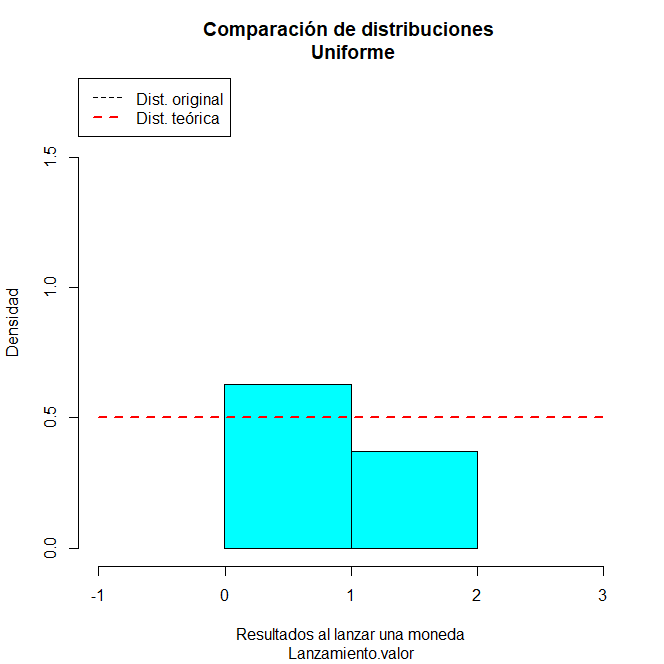
\includegraphics[scale=0.35]{Problema_80.png}
 \end{center}
 El cual coincide con los datos obtenidos,
 que es a lo que se quer\'{\i}a llegar.${}_{\blacksquare}$
\end{solucion}

 \newpage
 \item \begin{enunciado}
 Se supone que una m\'aquina mezcla cacahuates, avellanas, anacardos y pacanas
 a raz\'on de $5:2:2:1$.
 Se encuentra que una lata que contiene $500$ de tales nueces mezcladas tiene
 $269$ cacahuates, $112$ avellanas, $74$ anacardos y $45$ pacanas.
 Al nivel de significancia de $0.05$, pruebe la hip\'otesis
 de que la m\'aquina mezcla las nueces a una raz\'on de $5:2:2:1$.
\end{enunciado}

\begin{solucion}
 Para la soluci\'on, se va a definir una variable aleatoria $X$,
 que es una codificaci\'on de las nueces como $1,2,3$ y $4$
 para los cacahuates, las avellanas, los anacardos y las pecanas,
 respectivamente.
 As\'{\i}, pues, probar que la m\'aquina mezcla las nueces a una proporci\'on
 $5:2:2:1$ es equivalente a probar que $X$ sigue una distribuci\'on
 cuyos valores est\'an asignados como
 $f(x) = \frac{f_x}{f_1+f_2+f_3+f_4}$,
 para cada $x\in\mathbb{N}\cap[1,4]$ donde $f_X$
 es la frecuencia esperada, es decir,
 en este caso que se espera una raz\'on $5:2:2:1$, se puede 
 considerar $f_1=5$, $f_2=2$, $f_3=2$ y $f_4=1$,
 por lo que $f_1+f_2+f_3+f_4=5+2+2+1=10$ y
 $f(1)=\frac{5}{10}=\frac{1}{2}$,
 $f(2)=f(3)=\frac{2}{10}=\frac{1}{5}$
 y $f(4)=\frac{1}{10}$. 
 \begin{datos}
  $\phantom{0}$
  \begin{itemize}
   \item Tama\~no de la muestra: $n=500$.
   \item Frecuencias observadas:
   $O = \{ o_1 = 269, o_2 = 112, o_3 = 74, o_4 = 45 \}$.
   \item Probabilidades esperadas: $p_1 = \frac{1}{2}$,
   $p_2 = \frac{1}{5}$, $p_3 = \frac{1}{5}$ y $p_4 = \frac{1}{10}$
   \item frecuencias esperadas:
   $E = \left\{ e_i=n\cdot p_i \, | \forall\, i\in\mathbb{N}\cap[1,4] \right\} = \{ e_1 = 250, e_2 = 100, e_3 = 100, e_4 = 50 \}$.
   \item Celdas totales del experimento: $k=4$.
   \item Grados de libertad de la prueba $\chi^2$: $v = k-1 = 3$.
  \end{itemize}
 \end{datos}

 \begin{hipotesis}
  Prueba de bondad de ajuste para probar $H_0:$
  que una variable aleatoria $X$ de $4$ valores sigue una distribuci\'on
  con una raz\'on de $5:2:2:1$,
  contra la alternativa $H_1$ de que no es as\'{\i}.
 \end{hipotesis}

 \begin{estadistico}
  \begin{eqnarray*}
   \chi^2 & = & \sum_{i=1}^k \frac{\left( o_i - e_i \right)^2}{e_i}
   =\frac{(269 - 250)^2}{250} + \frac{(112 - 100)^2}{100} +
   \frac{(74-100)^2}{100} + \frac{(45-50)^2}{50} \\
   & = & \frac{19^2}{250} + \frac{12^2}{100} + \frac{26^2}{100} +
   \frac{5^2}{50}
   = \frac{361(2) + 144(5) + 676(5) + 25(10)}{500} = \frac{5\,072}{500}\\
   & = & \frac{1\,268}{125} = 10.144
  \end{eqnarray*}
 \end{estadistico}

 \begin{valorp}
  De la tabla A.5 se observa que $\chi^2_{0.02,3} \approx 9.837$
  $\chi^2_{0.01,3} \approx 11.345$,
  entonces, como $\chi^2_{0.02,3} < \chi^2 < \chi^2_{0.01,3}$,
  se sigue que el $P-$valor es un valor aproximadamente de $0.015$.
 \end{valorp}

 \begin{conclusion}
  Como el valor $P$ es muy peque\~no,
  se concluye que la muestra presentada es evidencia suficiente
  para rechazar la hip\'otesis nula y, por lo tanto, afirmar
  que la raz\'on en que la m\'aquina mezcla las nueces no es $5:2:2:1$.
 \end{conclusion}

 En el c\'odigo registrado en el archivo
 \texttt{P16\_Prueba\_de\_bondad\_chi2\_02.r}
 se realiza este procedimiento.
 El c\'odigo permite modificar los valores iniciales que corresponden a:
 \texttt{datos} que guarda los datos de la lectura de un archivo, en este caso se lee el archivo
 \texttt{DB17\_Problema\_081.csv},
 y este \'ultimo nombre es el que se modifica para leer otros archivos;
 \texttt{varInteres} para indicar el nombre de la columna
 que corresponde a los datos, agrupados ya en celdas
 y que, por lo tanto, aparece cada valor una \'unica vez en dicha columna;
 \texttt{varFrecuencia} para indicar el nombre de la columna
 de la frecuencia observada correspondiente a cada valor;
 \texttt{varProb} que indica el nombre de la columna
 que contiene la probabilidad esperada para cada valor;
 \texttt{combinar} para indicar, con \texttt{TRUE}, que,
 si la frecuencia esperada en alguna celda es menor a $5$,
 se combinen celdas, y aunque se puede indicar con \texttt{FALSE}
 que no se realice este proceso, el no realizarlo puede dar un error,
 por lo que es recomendarlo mantenerlo en \texttt{TRUE};
 \texttt{grafica} para indicar, con \texttt{TRUE}, que se realizar\'a
 una gr\'afica comparando las proporciones observadas
 de las probabilidades esperadas, o \texttt{FALSE}
 en caso de no graficar;
 \texttt{tituloEjeX} para indicar el t\'{\i}tulo en el eje X
 cuando se realice una gr\'afica;
 y, \texttt{alfa} para el nivel de confianza.
 \par 
 El programa espera al menos los datos correspondientes a la base de datos,
 escrito en un archivo \texttt{.csv} con una columna con los datos 
 correspondientes a los valores de las celdas, la frecuencia de cada valor
 y la probabilidad esperada para cada valor.
 \par 
 Este programa es una versi\'on resumida
 de \texttt{P16\_Prueba\_de\_bondad\_chi2\_02.r},
 en el que ahora se espera siempre los datos resumidos en celdas,
 adem\'as de requerir en la base de datos las probabilidades
 esperadas en vez de una distribuci\'on, permitiendo mayor robustes.
 Por otro lado, para la gr\'afica que realiza el programa
 se requiere del paquete \texttt{MASS}.
 \par 
 El resultado muestra lo siguiente:
 \texttt{Variable} que indica el nombre y unidad de lo que se est\'a midiendo;
 \texttt{Estad\'{\i}stico Chisq2} para el valor del estad\'{\i}stico
 $\chi^2$;
 \texttt{Grados de libertad} para indicar la cantidad de grados de libertad
 usado en los c\'alculos de probabilidades de la disitribuci\'on $\chi^2$;
 \texttt{Valor-p} para indicar el $p-$valor;
 \texttt{alpha} que muestra el valor asignado en la variable \texttt{alfa},
 \'o $0.05$ en caso de que se le haya asignado \texttt{NULL};
 \texttt{Región de Rechazo} que indica a partir de cu\'al valor
 del estad\'{\i}stico se rechaza la prueba,
 seg\'un el valor \texttt{alpha} mostrado;
 y, adem\'as, si se ha indicado un valor a la variable \texttt{alfa},
 entonces aparece \texttt{Resultado} para indicar si se rechaza
 o no la hip\'otesis nula.
 \par 
 El c\'odigo junto con el resultado se muestra a continuaci\'on:
 \begin{verbatim}
> require(MASS)
> datos<-read.csv("DB17_Problema_081.csv",sep=";",encoding="UTF-8")
> varInteres<-"Mezcla.nueces"
> varFrecuencia<-"Frecuencia"
> varProb<-"Probabilidad"
> combinar<-TRUE
> grafica<-TRUE
> tituloEjeX<-"Mezcla de varios tipos de nueces"
> alfa<-NULL
> valores<-datos[,varInteres]
> frecObs<-datos[,varFrecuencia]
> probEsp<-datos[,varProb]
> colapsar<-function(p1,f1,lim1=5){
+   np1<-p1
+   nf1<-f1
+   tocollapse<-which((np1*sum(nf1))<lim1)
+   while(length(tocollapse)>0){
+     x<-tocollapse[1]
+     if (x<length(np1)){
+       np1[x+1]<-p1[x]+p1[x+1]
+       nf1[x+1]<-f1[x]+f1[x+1]
+     }else{
+       np1[x-1]<-p1[x]+p1[x-1]
+       nf1[x-1]<-f1[x]+f1[x-1]
+     }
+     p1<-np1[-x]
+     f1<-nf1[-x]
+     np1<-p1
+     nf1<-f1
+     tocollapse<-which((p1*sum(f1))<lim1)
+   }
+   return(list(probs=p1,freqs=f1))  
+ }
> calculos<-function(frecObs,probEsp,alfa=0.05){
+   if(length(frecObs)>1){
+     r<-NULL
+     if(combinar){
+       r1<-colapsar(probEsp,frecObs)
+       frecObsC<-r1$freqs
+       probEspC<-r1$probs
+       if(length(frecObsC)>1){
+         prueba<-chisq.test(frecObsC,p=probEspC)
+       }else{
+         prueba<-NA
+       }
+     }else{
+       prueba<-chisq.test(frecObs,p=probEsp)
+     }
+     if(!is.na(prueba[1]) & prueba$parameter > 0){
+       r<-c(prueba$statistic, prueba$parameter,prueba$p.value,alfa,
+            qchisq(alfa,prueba$parameter,lower.tail=FALSE))
+     }
+     if(is.null(r)){
+       r<-rep(NA,5)
+     }
+     return(r)
+   }
+ }
> if(!is.null(alfa)){
+   tabla<-t(as.matrix(calculos(frecObs,probEsp,alfa)))
+ }else{
+   tabla<-t(as.matrix(calculos(frecObs,probEsp)))
+ }
> tabla<-data.frame(nombre=varInteres,tabla)
> names(tabla)<-c("Variable","Estadístico Chisq2",
+                 "Grados de libertad","Valor-p","alpha","Región de Rechazo")
> tabla["Región de Rechazo"]<-paste(">",round(tabla["Región de Rechazo"],7))
> generaGrafica<-function(valores,frecuencia,probEspG,tituloEjeX,nomVariable){
+   x<-c()
+   for(i in 1:length(valores)){
+     x<-c(x,rep(valores[i],frecuencia[i]))
+   }
+   maxD<-max(density(x)$y)
+   x11()
+   probEspG<-c(probEspG,0)
+   truehist(x,h=1,
+            main=paste("Comparación de distribuciones","\n","Específica"),
+            xlab=tituloEjeX, ylab="Densidad",sub=nomVariable,
+            xlim=c((min(x)-1),(max(x)+2)),
+            ymax=max(max(probEspG),maxD)*1.2)
+   lines((min(x)):(max(x)+1),probEspG,type="s",col="red",lty=2,lwd=2)
+   legend("topleft",legend = c("Dist. original", "Dist. teórica"),
+          lwd=c(1,2),lty=2,col=c("black","red"))
+   invisible()
+ }
> if(!is.null(alfa)){
+   tabla$alpha<-alfa
+   tabla$Resultado<-ifelse(tabla$"Valor-p">=alfa,
+                          "No se rechaza el ajuste de bondad",
+                          "Se rechaza el ajuste de bondad")
+ }
> tabla
       Variable Estadístico Chisq2 Grados de libertad    Valor-p alpha
1 Mezcla.nueces             10.144                  3 0.01738092  0.05
  Región de Rechazo
1       > 7.8147279
> if (grafica){
+   generaGrafica(valores,frecObs,probEsp,tituloEjeX,varInteres)
+ }
 \end{verbatim}
 \vspace{-0.5cm}
 que incluye la siguiente figura:
 \begin{center}
  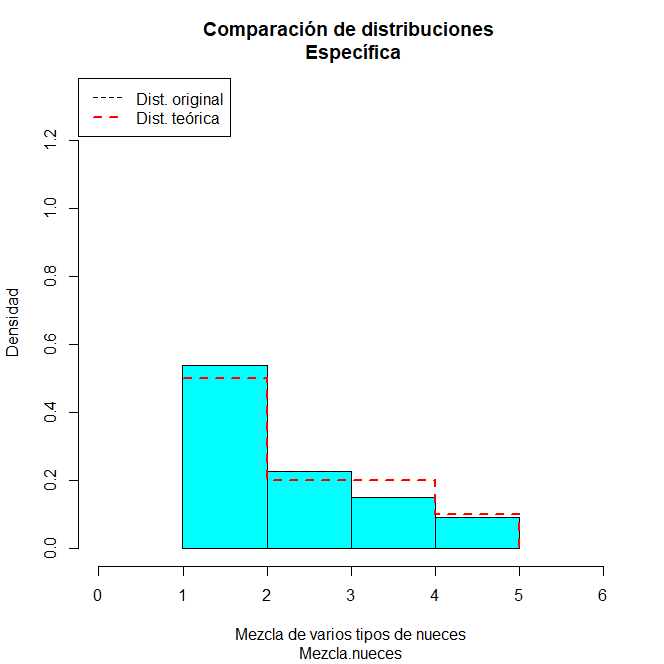
\includegraphics[scale=0.35]{Problema_81.png}
 \end{center}
 Lo cual coincide con los resultados obtenidos,
 que es a lo que se quer\'{\i}a llegar.${}_{\blacksquare}$
\end{solucion}

 \item \begin{enunciado}
 Considere una muestra de $x_1,x_2,\ldots,x_n$ observaciones de una distribuci\'on de Weibull con par\'ametros $\alpha$ y $\beta$ y funci\'on de densidad
 \begin{equation*}
  f(x) =
  \begin{cases}
   \alpha \beta x^{\beta - 1}e^{-\alpha x^{\beta}}, & x > 0, \\
   0, & \text{en cualquier otro caso,}
  \end{cases}
 \end{equation*}
 para $\alpha, \beta > 0$.
 \begin{enumerate}
  \item Escriba la funci\'on de probabilidad.
  \item Escriba las ecuaciones que al resolverse dan los estimadores de probabilidad m\'axima de $\alpha$ y $\beta$.
 \end{enumerate}
\end{enunciado}

\begin{solucion}
 $\phantom{0}$
 \begin{enumerate}
  \item Partiendo de la definici\'on de la funci\'on de probabilidad y dado que las muestras son independientes, entonces se tiene lo siguiente. 
  \begin{equation*}
   L\left( x_1, x_2, \ldots, x_n; \alpha, \beta \right) = \prod_{i=1}^n L\left( x_i; \alpha , \beta \right)
  \end{equation*}
  Entonces, si alguna muestra da un valor menor o igual que $0$, entonces la funci\'on de probabilidad es cero. En otro caso, se tiene que:
  \begin{eqnarray*}
   L\left( x_1, x_2, \ldots, x_n; \alpha, \beta \right) & = & \prod_{i=1}^{n} \alpha \beta x_i^{\beta - 1} e^{-\alpha x_i^\beta} \\
   & = & \alpha^n \beta^n \left( \prod_{i=1}^{n} x_i \right)^{\beta - 1} e^{-\alpha \sum_{i=1}^{n} x_i^\beta}._{\square}
  \end{eqnarray*}

  \item Por otro lado, para obtener las ecuaciones que den los estimadores de probabilidad m\'axima de $\alpha$ y $\beta$, convendr\'a calcular el logaritmo natural de la funci\'on de probabilidad como sigue:
  \begin{equation*}
   \ln L\left( x_1, x_2, \ldots, x_n; \alpha, \beta \right) = n\ln \alpha + n\ln \beta + (\beta - 1) \sum_{i=1}^{n} \ln x_i - \alpha \sum_{i=1}^n x_i^\beta
  \end{equation*}
  As\'{\i} que sus derivadas parciales son
  \begin{eqnarray*}
   \frac{\delta \ln L}{\delta \alpha} \left( x_1, x_2, \ldots, x_n; \alpha, \beta \right) & = & \frac{\delta}{\delta \alpha} \left( n\ln \alpha + \cancel{ n\ln \beta } + \cancel{ (\beta - 1) \sum_{i=1}^{n} \ln x_i } - \alpha \sum_{i=1}^n x_i^\beta \right) \\ 
   & = & \frac{n}{\alpha} - \sum_{i=1}^n x_i^\beta
  \end{eqnarray*}
  y
  \begin{eqnarray*}
   \frac{\delta \ln L}{\delta \beta} \left( x_1, x_2, \ldots, x_n; \alpha, \beta \right) & = & \frac{\delta}{\delta \beta} \left( \cancel{n\ln \alpha} + n\ln \beta + (\beta - 1) \sum_{i=1}^{n} \ln x_i - \alpha \sum_{i=1}^n x_i^\beta \right) \\ 
   & = & \frac{n}{\beta} + \sum_{i=1}^{n} \ln x_i - \alpha \sum_{i=1}^n x_i^\beta \ln x_i 
  \end{eqnarray*}
  Por otro lado, las derivadas parciales de segundo orden del logaritmo de la funci\'on de probabilidad son:
  \begin{eqnarray*}
   \frac{\delta^2 \ln L}{\delta \alpha^2} \left( x_1, x_2, \ldots, x_n; \alpha, \beta \right) & = & \frac{\delta}{\delta \alpha} \left( \frac{n}{\alpha} - \cancel{ \sum_{i=1}^n x_i^\beta } \right) \\
   & = & - \frac{n}{\alpha^2} \\
   \frac{\delta^2 \ln L}{\delta \beta \delta \alpha} \left( x_1, x_2, \ldots, x_n; \alpha, \beta \right) & = & \frac{\delta}{\delta \beta} \left( \cancel{ \frac{n}{\alpha} } - \sum_{i=1}^n x_i^\beta  \right) \\
   & = & - \sum_{i=1}^n x_i^\beta \ln x_i \\
   \frac{\delta^2 \ln L}{\delta \alpha \delta \beta} \left( x_1, x_2, \ldots, x_n; \alpha, \beta \right) & = & \frac{\delta}{\delta \alpha} \left( \cancel{ \frac{n}{\beta} } + \cancel{ \sum_{i=1}^{n} \ln x_i } - \alpha \sum_{i=1}^n x_i^\beta \ln x_i \right) \\ 
   & = & - \sum_{i=1}^n x_i^\beta \ln x_i
  \end{eqnarray*}
  y
  \begin{eqnarray*}
   \frac{\delta^2 \ln L}{\delta \beta^2} \left( x_1, x_2, \ldots, x_n; \alpha, \beta \right) & = & \frac{\delta}{\delta \beta} \left( \frac{n}{\beta} + \cancel{ \sum_{i=1}^{n} \ln x_i } - \alpha \sum_{i=1}^n x_i^\beta \ln x_i \right) \\ 
   & = & -\frac{n}{\beta^2} - \alpha \sum_{i=1}^n x_i^\beta \ln^2 x_i
  \end{eqnarray*}
  por lo que la matriz Hessiana del logaritmo de la funci\'on de probabilidad es:
  \begin{equation*}
   H_{\ln L(x_1,x_2, \ldots ,x_n; \alpha, \beta)} =
   \begin{bmatrix}
    \displaystyle{ - \frac{n}{\alpha^2} } & \displaystyle{ - \sum_{i=1}^n x_i^\beta \ln x_i } \\
    \displaystyle{ - \sum_{i=1}^n x_i^\beta \ln x_i } \quad & \displaystyle{ - \frac{n}{\beta^2} - \alpha \sum_{i=1}^n x_i^\beta \ln^2 x_i }
   \end{bmatrix}
  \end{equation*}
  Entonces, suponiendo que se tienen los estimadores de probabilidad m\'axima, $\hat{\alpha}$ y $\hat{\beta}$, se tiene que cumplir que las derivadas parciales de primer orden evaluados en estos estimadores son iguales a cero simult\'aneamente y, para comprobar que los estimadores son un punto m\'aximo, se debe cumplir que la Hessiana es definida negativamente, lo cual es equivalente a comprobar que el menor $|a_{1,1}| = a_{1,1}$ es negativo y el determinante es positivo. Como $n$ y $\alpha$ son positivos, entonces se cumple que $a_{1,1} = - \frac{n}{\alpha^2} < 0$, independientes de los valores de los estimadores, por lo que se reduce ahora a probar que el determinante de la Hessiana es positivo, el cual vale:
  \begin{equation*}
   \begin{vmatrix}
    \displaystyle{ - \frac{n}{\alpha^2} } & \displaystyle{ - \sum_{i=1}^n x_i^\beta \ln x_i } \\
    \displaystyle{ - \sum_{i=1}^n x_i^\beta \ln x_i } \quad & \displaystyle{ - \frac{n}{\beta^2} - \alpha \sum_{i=1}^n x_i^\beta \ln^2 x_i }
   \end{vmatrix}
   = \left( \frac{n}{\alpha \beta} \right)^2 + \frac{n}{\alpha} \sum_{i=1}^n x_i \ln^2 x_i - \left( \sum_{i=1}^n x_i^{\beta} \ln x_i \right)^2
  \end{equation*}
  Por lo tanto, los estimadores de m\'axima probabilidad, $\hat{\alpha}$ y $\hat{ \beta }$ de los par\'ametros $\alpha$ y $\beta$, respectivamente, deben cumplir las siguientes ecuaciones simmult\'aneamente:
  \begin{center}
   \begin{tabular}{lcr}
    $\displaystyle{ \frac{n}{\hat{ \alpha} } - \sum_{i=1}^n x_i^{\hat{\beta}} }$ & $=$ & $0$ \\
    $\displaystyle{ \frac{n}{\hat{\beta}} + \sum_{i=1}^{n} \ln x_i - \hat{\alpha} \sum_{i=1}^n x_i^{\hat{\beta}} \ln x_i }$ & $=$ & $0$ \\
    $\displaystyle{ \left( \frac{n}{\hat{\alpha} \hat{\beta}} \right)^2 + \frac{n}{\hat{\alpha}} \sum_{i=1}^n x_i \ln^2 x_i - \left( \sum_{i=1}^n x_i^{\hat{\beta}} \ln x_i \right)^2 }$ & $>$ & $0$
   \end{tabular}
  \end{center}
  que es a lo que se quer\'{\i}a llegar.${}_{\blacksquare}$
 \end{enumerate}
\end{solucion}

 \newpage
 \item \begin{enunciado}
 Considere la distribuci\'on logar\'{\i}tmica normal con la funci\'on de densidad dada en la secci\'on 6.9. Suponga que que tenemos una muestra $x_1, x_2, \ldots, x_n$ de una distribuci\'on logar\'{\i}tmica normal.
 \begin{enumerate}
  \item Escriba la funci\'on de probabilidad.
  \item Desarrolle los estimadores de probabilidad m\'axima de $\mu$ y $\sigma^2$.
 \end{enumerate}
\end{enunciado}

\begin{solucion}
 Recu\'erdese que la funci\'on de densidad logar\'{\i}tmica est\'a dada por
 \begin{equation*}
  f(x;\mu,\sigma^2) =
  \begin{cases}
   \frac{1}{\sqrt{2\pi}\sigma x}e^{-\frac{1}{2\sigma^2}\left[ \ln(x) - \mu \right]^2}, & x \geq 0, \\
   0, & x < 0
  \end{cases}
 \end{equation*}
 
 \begin{enumerate}
  \item A partir de la definici\'on de la funci\'on de densidad, si alguna muestra es menor a cero, se tiene que la funci\'on de densidad, y por lo tanto la funci\'on de probabilidad, es cero. Por lo tanto, suponiendo que ninguna muestra es menor a cero, se tiene que la funci\'on de probabilidad es:
  \begin{eqnarray*}
   L\left( x_1, x_2, \ldots, x_n; \mu, \sigma^2 \right) & = & \prod_{i=1}^n L\left( x_i; \mu, \sigma^2 \right) \\
   & = & \prod_{i=1}^n \frac{1}{\sqrt{2\pi \sigma^2} x_i}e^{-\frac{1}{2\sigma^2}\left[ \ln\left(x_i\right) - \mu \right]^2} \\
   & = & \frac{1}{(2\pi)^{n/2}\left( \sigma^2 \right)^{n/2} \prod_{i=1}^n x_i} e^{-\frac{1}{2\sigma^2} \sum_{i=1}^n \left[ \ln\left( x_i \right) - \mu \right]^2}._{\square}
  \end{eqnarray*}
  
  \item Por otro lado, para obtener las ecuaciones que den los estimadores de probabilidad m\'axima de $\mu$ y $\sigma^2$, convendr\'a calcular el logaritmo natural de la funci\'on de probabilidad como sigue:
  \begin{equation*}
   \ln L \left( x_1, x_2, \ldots, x_n; \mu, \sigma^2 \right) = -\frac{n}{2}\ln(2\pi) - \frac{n}{2}\ln\left( \sigma^2 \right) - \sum_{i=1}^2 x_i - \frac{1}{2\sigma^2} \sum_{i=1}^n \left[ \ln\left( x_i \right) - \mu \right]^2
  \end{equation*}
  As\'{\i} que sus derivadas parciales son
  \begin{eqnarray*}
   \frac{\delta \ln L}{\delta \mu} \left( x_1, x_2, \ldots, x_n; \mu, \sigma^2 \right) & = & \\
   & & \hspace{-0.5cm} \frac{\delta}{\delta \mu} \left( \cancel{ -\frac{n}{2}\ln(2\pi) } - \cancel{ \frac{n}{2}\ln\left( \sigma^2 \right) } - \cancel{ \sum_{i=1}^2 x_i } - \frac{1}{2\sigma^2} \sum_{i=1}^n \left[ \ln\left( x_i \right) - \mu \right]^2 \right) \\
   & = & \frac{\sum_{i=1}^n \ln\left( x_i \right) - n\mu}{\sigma^2}
  \end{eqnarray*}
  y
  \begin{eqnarray*}
   \frac{\delta \ln L}{\delta \sigma^2} \left( x_1, x_2, \ldots, x_n; \mu, \sigma^2 \right) & = & \\
   & & \hspace{-0.5cm} \frac{\delta}{\delta \sigma^2} \left( \cancel{ -\frac{n}{2}\ln(2\pi) } - \frac{n}{2}\ln\left( \sigma^2 \right) - \cancel{ \sum_{i=1}^2 x_i } - \frac{1}{2\sigma^2} \sum_{i=1}^n \left[ \ln\left( x_i \right) - \mu \right]^2 \right) \\
   & = & - \frac{n}{2\sigma^2} + \frac{\sum_{i=1}^n \left[ \ln\left( x_i \right) - \mu \right]^2}{2\left( \sigma^2 \right)^2}
  \end{eqnarray*}
  Por otro lado, las derivadas parciales de segundo orden del logaritmo de la funci\'on de probabilidad son:
  \begin{eqnarray*}
   \frac{\delta^2 \ln L}{\delta \mu^2} \left( x_1, x_2, \ldots, x_n; \mu, \sigma^2 \right) & = & \frac{\delta}{\delta \mu} \left( \frac{\cancel{ \sum_{i=1}^n \ln\left( x_i \right) } - n\mu}{\sigma^2} \right) \\
   & = & - \frac{n}{\sigma^2} \\
   \frac{\delta^2 \ln L}{\delta \sigma^2 \delta \mu} \left( x_1, x_2, \ldots, x_n; \mu, \sigma^2 \right) & = & \frac{\delta}{\delta \sigma^2} \left( \frac{\sum_{i=1}^n \ln\left( x_i \right) - n\mu}{\sigma^2} \right) \\
   & = & \frac{n\mu - \sum_{i=1}^n \ln x_i}{\left( \sigma^2 \right)^2} \\
   \frac{\delta^2 \ln L}{\delta \left( \sigma^2 \right)^2} \left( x_1, x_2, \ldots, x_n; \mu, \sigma^2 \right) & = & \frac{\delta}{\delta \sigma^2} \left( - \frac{n}{2\sigma^2} + \frac{\sum_{i=1}^n \left[ \ln\left( x_i \right) - \mu \right]^2}{2\left( \sigma^2 \right)^2} \right) \\
   & = & \frac{n}{2\left( \sigma^2 \right)^2} - \frac{\sum_{i= 1}^n \left[ \ln\left( x_i \right) - \mu \right]^2}{\left( \sigma^2 \right)^3} \\
   & = & \frac{n\sigma^2 - 2\sum_{i=1}^n \left[ \ln\left( x_i \right) - \mu \right]^2}{2\left( \sigma^2 \right)^3} 
  \end{eqnarray*}
  y
  \begin{eqnarray*}
   \frac{\delta^2 \ln L}{\delta \mu \delta \sigma^2} \left( x_1, x_2, \ldots, x_n; \mu, \sigma^2 \right) & = & \frac{\delta}{\delta \mu} \left( \cancel{ - \frac{n}{2\sigma^2} } + \frac{\sum_{i=1}^n \left[ \ln\left( x_i \right) - \mu \right]^2}{2\left( \sigma^2 \right)^2} \right) \\
   & = & \frac{n\mu - \sum_{i=1}^n \ln x_i}{\left( \sigma^2 \right)^2}
  \end{eqnarray*}
  por lo que la Hessiana del logaritmo de la funci\'on de probabilidad es:
  \begin{equation*}
   H_{\ln L \left( x_1, x_2, \ldots, x_n; \mu, \sigma^2 \right)} =
   \begin{bmatrix}
    \displaystyle{ - \frac{n}{\sigma^2} } & \displaystyle{ \frac{n\mu - \sum_{i=1}^n \ln x_i}{\left( \sigma^2 \right)^2} } \\
    \displaystyle{ \frac{n\mu - \sum_{i=1}^n \ln x_i}{\left( \sigma^2 \right)^2} } & \displaystyle{ \frac{n\sigma^2 - 2\sum_{i=1}^n \left[ \ln\left( x_i \right) - \mu \right]^2}{2\left( \sigma^2 \right)^3} }
   \end{bmatrix}
  \end{equation*}
  Entonces, los estimadores de probabilidad m\'axima, $\hat{\mu}$ y $\widehat{\sigma^2}$, cumplen que al evaluarse sobre las derivadas parciales de primer orden, estas se hacen cero, y, adem\'as, la Hessiana es definida negativamente. Para que esto primero se cumpla, se tiene lo siguiente, en donde $y_i = \ln x_i$:
  \begin{eqnarray*}
   \frac{\sum_{i=1}^n \ln\left( x_i \right) - n\hat{\mu}}{\widehat{\sigma^2}} = 0 & \Leftrightarrow & \sum_{i=1}^n \ln\left( x_i \right) - n\hat{\mu} = 0 \\
   & \Leftrightarrow & n\hat{\mu} = \sum_{i=1}^n \ln\left( x_i \right) \\
   & \Leftrightarrow & \hat{\mu} = \frac{\sum_{i=1}^n \ln\left( x_i \right)}{n} \\
   & \Leftrightarrow & \hat{\mu} = \frac{\sum_{i=1}^n y_i}{n} = \bar{y}
  \end{eqnarray*}
  y
  \begin{eqnarray*}
   - \frac{n}{2\widehat{\sigma^2}} + \frac{\sum_{i=1}^n \left[ \ln\left( x_i \right) - \hat{\mu} \right]^2}{2\left( \widehat{\sigma^2} \right)^2} = 0 & \Leftrightarrow & \frac{\sum_{i=1}^n \left[ \ln\left( x_i \right) - \hat{\mu} \right]^2 - n\widehat{\sigma^2}}{2\left( \widehat{\sigma^2} \right)^2} = 0 \\
   & \Leftrightarrow & \sum_{i=1}^n \left[ \ln\left( x_i \right) - \hat{\mu} \right]^2 - n\widehat{\sigma^2} = 0 \\
   & \Leftrightarrow & n\widehat{\sigma^2} = \sum_{i=1}^n \left[ \ln\left( x_i \right) - \hat{\mu} \right]^2 \\
   & \Leftrightarrow & \widehat{\sigma^2} = \frac{\sum_{i=1}^n \left[ \ln\left( x_i \right) - \hat{\mu} \right]^2}{n} = \frac{1}{n} \sum_{i=1}^n \left( y_i - \bar{y} \right)^2
  \end{eqnarray*}
  y, al evaluar la Hessiana en estos puntos, se tiene que:
  \begin{eqnarray*}
   \begin{bmatrix}
    \displaystyle{ - \frac{n}{\widehat{\sigma^2}} } & \displaystyle{ \frac{n\hat{\mu} - \sum_{i=1}^n \ln x_i}{\left( \widehat{ \sigma^2 } \right)^2} } \\
    \displaystyle{ \frac{n\hat{\mu} - \sum_{i=1}^n \ln x_i}{\left( \widehat{ \sigma^2 } \right)^2} } & \displaystyle{ \frac{n\widehat{ \sigma^2 } - 2\sum_{i=1}^n \left[ \ln\left( x_i \right) - \hat{\mu} \right]^2}{2\left( \widehat{ \sigma^2 } \right)^3} }
   \end{bmatrix}
   & = & 
   \begin{bmatrix}
    \displaystyle{ -\frac{n^2}{\sum_{i=1}^n \left( y_i - \bar{y} \right)^2 } } & \displaystyle{ \frac{ \cancel{n\bar{y} - n\bar{y}} }{\left( \widehat{\sigma^2} \right)^2} } \\
    \displaystyle{ \frac{ \cancel{n\bar{y} - n\bar{y}} }{\left( \widehat{\sigma^2} \right)^2} } & \displaystyle{ \frac{n\widehat{\sigma^2} - 2n\widehat{\sigma^2}}{2\left( \widehat{\sigma^2} \right)^3} }
   \end{bmatrix}
   \\
   & = &
   \begin{bmatrix}
    \displaystyle{ -\frac{n^2}{\sum_{i=1}^n \left( y_i - \bar{y} \right)^2 } } & 0 \\
    0 & - \frac{n}{2\left( \widehat{\sigma^2} \right)^2}
   \end{bmatrix}
  \end{eqnarray*}
  por lo que la Hessiana en este punto resulta ser una matriz diagonal, por lo que sus autovalores son iguales a los elementos en su diagonal, lo cual indica que todos los autovalores de la Hessiana son negativos y, por lo tanto, la Hessiana es definida negativa. Por lo tanto, el logaritmo de la funci\'on de probabilidad es estrictamente c\'oncava en el punto $\left( \hat{\mu} , \widehat{\sigma^2} \right)$. Por lo tanto, con todo lo anterior, se tiene que:
  \begin{eqnarray*}
   \hat{\mu} & = & \frac{1}{n} \sum_{i=1}^n \ln x_i \\
   \widehat{\sigma^2} & = & \frac{1}{n} \sum_{i=1}^n \left[ \ln\left( x_i \right) - \left( \frac{1}{n} \sum_{i=1}^n \ln x_i \right) \right]^2
  \end{eqnarray*}
  son los estimadores de m\'axima probabilidad, que es a lo que se quer\'{\i}a llegar.${}_{\blacksquare}$
 \end{enumerate}
\end{solucion}

 \item \begin{enunciado}
 Considere las observaciones $x_1, x_2, \ldots, x_n$ de la distribuci\'on gamma que se discuti\'o en la secci\'on 6.6.
 \begin{enumerate}
  \item Escriba la funci\'on de probabilidad.
  \item Escriba un conjunto de ecuaciones que cuando se resuelvan den los estimadores de probabilidad m\'axima de $\alpha$ y $\beta$.
 \end{enumerate}
\end{enunciado}

\begin{solucion}
 Recu\'erdese que la funci\'on de densidad gamma est\'a dada por
 \begin{equation*}
  f(x; \alpha, \beta) =
  \begin{cases}
  \frac{1}{\beta^{\alpha} \Gamma(\alpha)} x^{\alpha-1} e^{-x/\beta} , & x > 0 \\
  0, & \text{en cualquier otro caso},
  \end{cases}
 \end{equation*}
 donde $\alpha > 0$ y $\beta > 0$, y en donde la funci\'on gamma, $\Gamma(\alpha)$, se define como
 \begin{equation*}
  \Gamma(\alpha) = \int_0^{\infty} x^{\alpha - 1} e^{-x} \, dx
 \end{equation*}
 para $\alpha > 0$. Adem\'as, se tienen varias propiedades de la funci\'on Gamma, algunas de ellas se encuentran enlistadas en el \textit{Anexo 02.pdf}, entre las que se destacar\'an para este problema el hecho que $\Gamma \in C^{\infty}$; adem\'as, se define la funci\'on psi, o digamma, como:
 \begin{equation*}
  \psi(x) = \frac{\delta}{\delta x} \ln\left( \Gamma(x) \right) = \frac{\Gamma'(x)}{\Gamma(x)}
 \end{equation*}
 y las funciones poligamma como:
 \begin{eqnarray*}
  \psi^{(0)}(x) & = & \psi(x), \qquad \text{y} \\
  \psi^{(n)}(x) & = & \psi^{(n)}(x) = \frac{\delta}{\delta x} \psi^{(n-1)}, \qquad \forall n \in \mathbb{N}
 \end{eqnarray*}
 Una representaci\'on de la funci\'on digamma como una integral queda definida gracias a la expresi\'on de la funci\'on Gamma como el producto:
 \begin{equation*}
  \Gamma(\alpha+1) = e^{-\gamma z} \prod_{n\in\mathbb{N}} \left( 1 + \frac{\alpha}{n} \right)^{-1} e^{\alpha/n}
 \end{equation*}
 en donde $\gamma$ representa la constante de Euler-Mascheroni, definido como
 \begin{equation*}
  \gamma = \sum_{k=1}^{\infty} \left[  \frac{1}{k} - \ln\left( 1 + \frac{1}{k} \right) \right] = \int_{1}^{\infty} \left( \frac{1}{\lfloor x \rfloor} - \frac{1}{x} \right) \, dx
 \end{equation*}
 aunque tambi\'en se puede obtener bajo la relaci\'on $\gamma = -\Gamma'(1)$, y cuyo valor es aproximadamente $0.5772\ldots$.
 \par
 Entonces se obtiene que
 \begin{equation*}
  \psi(\alpha + 1) = - \gamma + \sum_{n\in\mathbb{N}} \left( \frac{1}{n} - \frac{1}{\alpha + n} \right) = \sum_{n\in\mathbb{N}} \left[ \ln(n+1) - \ln(n) + \frac{1}{n+\alpha} \right]
 \end{equation*}
 y por la transformaci\'on inversa de Laplace y el teorema de Frullani, se tiene que
 \begin{equation*}
  \ln(n+1) - \ln(n) = \int_{0}^{\infty} \frac{e^{-nt} - e^{-(n+1)t}}{t} \, dt, \qquad \text{ y } \qquad \frac{1}{n + \alpha} = \int_{0}^{\infty} e^{-(n+\alpha)t} \, dt
 \end{equation*}
 Luego, bajo la manipulaci\'on adecuada, se obtiene que una representaci\'on como una \'unica integral de la funci\'on digamma es:
 \begin{equation*}
  \psi(\alpha) = \int_{0}^{\infty} \left( \frac{e^{-t}}{t} - \frac{e^{-\alpha t}}{1 - e^{-t}} \right) \, dt
 \end{equation*}
 Por otro lado, se puede demostrar que la funci\'on poligamma se puede representar como
 \begin{equation*}
  \psi^{(n)} (\alpha) = (-1)^{n+1} \int_{0}^{\infty} \frac{t^{n}e^{-\alpha t}}{1-e^{-t}} \, dt
 \end{equation*}
 para $n \in \mathbb{N}$.
 \begin{enumerate}
  \item A partir de la definici\'on de la funci\'on de densidad, si alguna muestra es menor o igual que cero, se tiene que la funci\'on de densidad, y por lo tanto la funci\'on de probabilidad, es cero. Por lo tanto, suponiendo que ninguna muestra es menor o igual que cero, se tiene que la funci\'on de probabilidad es:
  \begin{eqnarray*}
   L\left( x_1, x_2, \ldots, x_n; \alpha, \beta \right) & = & \prod_{i=1}^n L\left( x_i; \alpha, \beta \right) \\
   & = & \prod_{i=1}^n \frac{1}{\beta^{\alpha} \Gamma(\alpha)} x_i^{\alpha-1} e^{-x_i/\beta} \\
   & = & \frac{1}{\beta^{n\alpha}\left[ \Gamma(\alpha) \right]^n} \left( \prod_{i=1}^n x_i \right)^{\alpha-1} e^{-\frac{1}{\beta}\sum_{i=1}^n x_i}._{\square}
  \end{eqnarray*}
  
  \item Por otro lado, para obtener las ecuaciones que den los estimadores de probabilidad m\'axima de $\alpha$ y $\beta$, convendr\'a calcular el logaritmo natural de la funci\'on de probabilidad como sigue:
  \begin{equation*}
   \ln L \left( x_1, x_2, \ldots, x_n; \alpha, \beta \right) = -n\alpha \ln \beta - n\ln \left[ \Gamma(\alpha) \right] + (\alpha-1)\sum_{i=1}^n \ln x_i - \frac{1}{\beta} \sum_{i=1}^n x_i
  \end{equation*}
  As\'{\i} que sus derivadas parciales son
  \begin{eqnarray*}
   \frac{\delta \ln L}{\delta \alpha} \left( x_1, x_2, \ldots, x_n; \alpha, \beta \right) & = & \frac{\delta}{\delta \alpha} \left( -n\alpha \ln \beta - n\ln \left[ \Gamma(\alpha) \right] + (\alpha-1)\sum_{i=1}^n \ln x_i - \cancel{ \frac{1}{\beta} \sum_{i=1}^n x_i } \right) \\
   & = & -n\ln \beta - \frac{n}{\Gamma(\alpha)} \cdot \frac{\delta \Gamma(\alpha)}{\delta \alpha} + \sum_{i=1}^n \ln x_i \\
   & = & -n\ln \beta - n\psi(\alpha) + \sum_{i=1}^{n} \ln x_i
  \end{eqnarray*}
  y
  \begin{eqnarray*}
   \frac{\delta \ln L}{\delta \beta} \left( x_1, x_2, \ldots, x_n; \alpha, \beta \right) & = & \frac{\delta}{\delta \beta} \left( -n\alpha \ln \beta - \cancel{ n\ln \left[ \Gamma(\alpha) \right] }  + \cancel{ (\alpha-1)\sum_{i=1}^n \ln x_i } - \frac{1}{\beta} \sum_{i=1}^n x_i \right) \\
   & = & - \frac{n\alpha}{\beta} + \frac{\sum_{i=1}^n x_i}{\beta^2}
  \end{eqnarray*}
  Por otro lado, las derivadas parciales de segundo orden del logaritmo de la funci\'on de probabilidad son:
  \begin{eqnarray*}
   \frac{\delta^2 \ln L}{\delta \alpha^2} \left( x_1, x_2, \ldots, x_n; \alpha, \beta \right) & = & \frac{\delta}{\delta \alpha} \left( \cancel{-n\ln \beta} - n\psi(\alpha) + \cancel{\sum_{i=1}^{n} \ln x_i} \right) \\
   & = &  = -n\psi^{(1)}(\alpha) \\
   \frac{\delta^2 \ln L}{\delta \beta \delta\alpha} \left( x_1, x_2, \ldots, x_n; \alpha, \beta \right) & = & \frac{\delta}{\delta \beta} \left( -n\ln \beta - \cancel{n\psi(\alpha) + \sum_{i=1}^{n} \ln x_i} \right) \\
   & = & -\frac{n}{\beta} \\
   \frac{\delta^2 \ln L}{\delta \alpha \delta\beta} \left( x_1, x_2, \ldots, x_n; \alpha, \beta \right) & = & \frac{\delta}{\delta \alpha} \left( - \frac{n\alpha}{\beta} + \cancel{ \frac{\sum_{i=1}^n x_i}{\beta^2} } \right) \\
   & = & -\frac{n}{\beta}
  \end{eqnarray*}
  y
  \begin{eqnarray*}
   \frac{\delta^2 \ln L}{\delta^2 \beta} \left( x_1, x_2, \ldots, x_n; \alpha, \beta \right) & = & \frac{\delta}{\delta \beta} \left( - \frac{n\alpha}{\beta} + \frac{\sum_{i=1}^n x_i}{\beta^2} \right) \\
   & = & \frac{n\alpha}{\beta^2} - \frac{2\sum_{i=1}^{n} x_i }{\beta^3} \\
   & = & \frac{n\alpha\beta - 2\sum_{i=1}^n x_i}{\beta^3}
  \end{eqnarray*}
  por lo que la Hessiana del logaritmo de la funci\'on de probabilidad es:
  \begin{equation*}
   H_{\ln L} \left( x_1, x_2, \ldots, x_n; \alpha, \beta \right) =
   \begin{bmatrix}
    -n\psi^{(1)}(\alpha) & \displaystyle{ -\frac{n}{\beta} } \\
    \displaystyle{ -\frac{n}{\beta} } & \displaystyle{ \frac{n\alpha\beta - 2\sum_{i=1}^n x_i}{\beta^3} }
   \end{bmatrix}
  \end{equation*}
  Entonces, los estimadores de probabilidad m\'axima, $\widehat{\alpha}$ y $\widehat{\beta}$, cumplen que al evaluarse sobre las derivadas parciales de primer orden, \'estas se hacen cero, y, adem\'as, la Hessiana es definida negativamente. Para que esto primero se cumpla, se tiene lo siguiente:
  \begin{eqnarray*}
   -n\ln \widehat{\beta} - n\psi\left(\widehat{\alpha}\right) + \sum_{i=1}^{n} \ln x_i = 0 & \Leftrightarrow & n\left( \ln \widehat{\beta} + \psi\left(\widehat{\alpha}\right) \right) = \sum_{i=1}^n x_i \\
   & \Leftrightarrow & \ln \widehat{\beta} + \psi\left(\widehat{\alpha}\right) = \frac{1}{n} \sum_{i=1}^{n} \ln x_i
  \end{eqnarray*}
  y
  \begin{eqnarray*}
   - \frac{n\widehat{\alpha}}{\widehat{\beta}} + \frac{\sum_{i=1}^n x_i}{\widehat{\beta}^2} = 0 & \Leftrightarrow & \frac{ \sum_{i=1}^n x_i - n\widehat{\alpha}\widehat{\beta}}{\widehat{\beta}^2} = 0 \\
   & \Leftrightarrow & \sum_{i=1}^n x_i = n\widehat{\alpha}\widehat{\beta} \\
   & \Leftrightarrow & \widehat{\alpha}\widehat{\beta} = \frac{1}{n}\sum_{i=1}^n x_i
  \end{eqnarray*}
  y, al evaluar la Hessiana en estos puntos se tiene que:
  \begin{eqnarray*}
   \begin{bmatrix}
    -n\psi^{(1)}\left(\widehat{\alpha}\right) & \displaystyle{ -\frac{n}{\widehat{\beta}} } \\
    \displaystyle{ -\frac{n}{\widehat{\beta}} } & \displaystyle{ \frac{n\widehat{\alpha}\widehat{\beta} - 2\sum_{i=1}^n x_i}{\widehat{\beta}^3} }
   \end{bmatrix}
   & = & 
   \begin{bmatrix}
    -n\psi^{(1)}\left(\widehat{\alpha}\right) & \displaystyle{ -\frac{n}{\widehat{\beta}} } \\
    \displaystyle{ -\frac{n}{\widehat{\beta}} } & \displaystyle{ \frac{n\widehat{\alpha}\widehat{\beta} - 2n\widehat{\alpha}\widehat{\beta}}{\widehat{\beta}^3} }
   \end{bmatrix}
   \\
   & = &
   \begin{bmatrix}
    -n\psi^{(1)}\left(\widehat{\alpha}\right) & \displaystyle{ -\frac{n}{\widehat{\beta}} } \\
    \displaystyle{ -\frac{n}{\widehat{\beta}} } & \displaystyle{ - \frac{n\widehat{\alpha}}{\widehat{\beta}^2} }
   \end{bmatrix}
  \end{eqnarray*}
  demostrar que la Hessiana es definida negativamente es equivalente a comprobar que el determinante $\left| a_{1,1} \right| = a_{1,1}$ es negativo y que el determinante de la Hessiana es positivo. Como $n$ y $\psi^{(1)}\left( \widehat{\alpha} \right)$ son positivos, para todo $\alpha > 0$, entonces se cumple que $a_{1,1} = -n\psi^{(1)}(\alpha) < 0$, y, como adem\'as $\alpha$ y $\beta$ son positivos, entonces
  \begin{equation*}
   \begin{vmatrix}
    -n\psi^{(1)}\left(\widehat{\alpha}\right) & \displaystyle{ -\frac{n}{\widehat{\beta}} } \\
    \displaystyle{ -\frac{n}{\widehat{\beta}} } & \displaystyle{ - \frac{n\widehat{\alpha}}{\widehat{\beta}^2} }
   \end{vmatrix} 
   = \frac{n^2\alpha\psi^{(1)}(\alpha)}{\beta^2} + \frac{n^2}{\beta^2} = \frac{n^2\left( \alpha\psi^{(1)}(\alpha) + 1 \right)}{\beta^2}
  \end{equation*}
  es positivo si y s\'olo si
  \begin{equation*}
   \alpha\psi^{(1)}(\alpha) + 1 > 0
  \end{equation*}
  lo cual ocurre siempre para los estimadores que cumplen la condici\'on de igualdad en cero de la primera derivada. Por lo tanto la Hessiana que cumple las primeras condiciones, siempre es negativo.
  \par 
  Por lo tanto, los estimadores de m\'axima probabilidad, $\widehat{\alpha}$ y $\widehat{\beta}$ de los par\'ametros $\alpha$ y $\beta$, respectivamente, deben cumplir las siguientes ecuaciones simult\'aneamente:
  \begin{eqnarray*}
   \ln \widehat{\beta} + \psi\left(\widehat{\alpha}\right) & = & \frac{1}{n} \sum_{i=1}^{n} \ln x_i \\
   \widehat{\alpha}\widehat{\beta} & = & \frac{1}{n}\sum_{i=1}^n x_i
  \end{eqnarray*}
  que es a lo que se quer\'{\i}a llegar.${}_{\blacksquare}$
 \end{enumerate}
\end{solucion}

 \item \begin{enunciado}
 Se lanza una moneda hasta que sale una cara y se registra el n\'umero
 de lanzamientos $X$.
 Despu\'es de repetir el experimento $256$ veces,
 obtenemos los siguientes resultados:
 \begin{center}
  \begin{tabular}{c|cccccccc}
   $x$ &  $1$  &  $2$ &  $3$ &  $4$ & $5$ & $6$ & $7$ & $8$ \\
   $f$ & $136$ & $60$ & $34$ & $12$ & $9$ & $1$ & $3$ & $1$
  \end{tabular}
 \end{center}
 Con un nivel de significancia de $0.05$ pruebe la hip\'otesis
 de que la distribuci\'on observada de $X$ se puede ajustar
 por la distribuci\'on geom\'etrica $g(x;1/2)$, $x = 1,2,3,\ldots$
\end{enunciado}

\begin{solucion}
 \begin{datos}
  $\phantom{0}$
  \begin{itemize}
   \item Tama\~no de la muestra: $n=256$.
   \item Frecuencias observadas:
   $O = \{o_1=136, o_2=60, o_3=34, o_4=12, o_5=9, o_6=1, o_7=3, o_8=1\}$.
   \item Probabilidades esperadas: como distribuci\'on geom\'etrica
   est\'a definida para cada $x\in\mathbb{N}$, entones $p_i = g(i;1/2) =
   \frac{1}{2} \cdot \left( \frac{1}{2} \right)^{i-1} = 
   \left( \frac{1}{2} \right)^{i} = \frac{1}{2^i}$,
   para cada $i \in \mathbb{N}\cap[1,7]$
   y $p_8 = g(x\geq 8; 1/2) = 1 - \sum_{i=1}^{7} g(i;1/2)
   = 1 - \sum_{i=1}^{7} p_i$.
   Entonces $p_1 = \frac{1}{2}$, $p_2 = \frac{1}{4}$, $p_3 = \frac{1}{8}$,
   $p_4 = \frac{1}{16}$, $p_5 = \frac{1}{32}$, $p_6 = \frac{1}{64}$,
   $p_7 = \frac{1}{128}$
   y, como $\sum_{i=1}^7 p_i=\frac{64+32+16+8+4+2+1}{128}=\frac{127}{128}$, entonces $p_8 = 1 - \frac{127}{128} = \frac{1}{128}$.
   \item Frecuencias esperadas: $E = \left\{
   \left.e_i=n\cdot p_i\,\right|\,\forall i\in\mathbb{N} \right\}
   = \{e_1=128, e_2=64, e_3=32, e_4=16, e_5=8, e_6=4, e_7=2, e_8=2\}$.
  \end{itemize}
  Dado que las pruebas de bondad por m\'etodo de $\chi^2$ no son confiables
  cuando la frecuencia esperada de una celda es menor a $5$,
  se agrupar\'an los datos, como sigue:
  \begin{itemize}
   \item Probabilidades esperadas:
   $\{ p_1 = \frac{1}{2}, p_2 = \frac{1}{4}, p_3 = \frac{1}{8},
   p_4 = \frac{1}{16}, p_5 = \frac{1}{32}, p_6 = \frac{1}{32} \}$.
   \item Frecuencias esperadas:
   $E=\{e_1 = 128, e_2 = 64, e_3 = 32, e_4 = 16, e_5 = 8, e_6 = 8\}$.
   \item Frecuencias observadas:
   $O = \{o_1=136, o_2=60, o_3=34, o_4=12, o_5=9, o_6=5\}$.
   \item Celdas totales del experimento: $k=6$.
   \item Grados de libertad de la prueba $\chi^2$: $v= k-1 = 5$.
  \end{itemize}
 \end{datos}

 \begin{hipotesis}
  Prueba de bondad de ajuste para probar $H_0:$
  que la variable aleatoria $X$, del n\'umero veces
  que se lanz\'o la moneda del enunciado hasta obtener la primera cara,
  sigue una distribuci\'on geom\'etrica
  con par\'ametro $p=\frac{1}{2}$,
  contra la alternativa $H_1$ de que no es as\'{\i}.
 \end{hipotesis}

 \begin{significancia}
  $\alpha = 0.05$.
 \end{significancia}

 \begin{region}
  De la tabla A.5 se tiene el valor cr\'{\i}tico
  $\chi^2_{\alpha,v} = \chi^2_{0.05,5} \approx 11.07$,
  por lo que la regi\'on de rechazo est\'a dado
  para $\chi^2 > 11.07$, donde
  $\chi^2 = \sum_{i=1}^{k} \frac{\left( o_i - e_i \right)^2}{e_i}$.
 \end{region}

 \begin{estadistico}
  \begin{eqnarray*}
   \chi^2 & = & \sum_{i=1}^{k} \frac{\left( o_i - e_i \right)^2}{e_i} \\
   & = & \frac{(136-128)^2}{128} + \frac{(60-64)^2}{64} +
   \frac{(34-32)^2}{32} + \frac{(12-16)^2}{16} +
   \frac{(9-8)^2}{8} + \frac{(5-8)^2}{8} \\
   & = &
   \frac{8^2 + 4^2(2) + 2^2(4) + 4^2(8) + 1^2(16) + 3^2(16)}{128}\\
   & = & \frac{64 + 32 + 16 + 128 + 16 + 144}{128} = \frac{400}{128} \\
   & = & \frac{25}{8} = 3.125
  \end{eqnarray*}
 \end{estadistico}

 \begin{decision}
  No se rechaza $H_0$.
 \end{decision}

 \begin{conclusion}
  No hay evidencia suficiente para rechazar que el experimento
  de lanzar un moneda hasta obtener una cara con la moneda del enunciado
  sea una distribuci\'on distinta de la geom\'etrica
  con par\'ametro $p=\frac{1}{2}$;
  es decir, no se confirma que el experimento no es significativamente
  distinto de esta distribuci\'on.
 \end{conclusion}

 Finalmente, usando el archivo anexo
 \texttt{P15\_Prueba\_de\_bondad\_chi2\_01.r},
 que a su vez requiere los datos del archivo
 \texttt{DB21\_Problema\_085.csv}, con los siguientes cambios:
 \begin{verbatim}
> datos<-read.csv("DB21_Problema_085.csv",sep=";",encoding="UTF-8")
> varInteres<-"Frecuencia"
> varCelda<-"Lanzamientos.cantidad"
> distribucion<-4
> parametro_nombre<-c("p")
> parametro_valor<-c(1/2)
> combinar<-TRUE
> grafica<-TRUE
> tituloEjeX<-"Primera aparición de cara en los lanzamientos de una moneda"
> alfa<-0.05
 \end{verbatim}
 \vspace{-0.7cm}
 el programa de R lanza el siguiente resultado:
 \begin{verbatim}
               Variable Distribución de ajuste   p Estadístico Chisq2
1 Lanzamientos.cantidad             Geométrica 0.5              3.125
  Grados de libertad   Valor-p alpha Región de Rechazo
1                  5 0.6807215  0.05      > 11.0704977
                          Resultado
1 No se rechaza el ajuste de bondad
 \end{verbatim}
 \vspace{-0.7cm}
 que incluye la siguiente figura:
 \begin{center}
  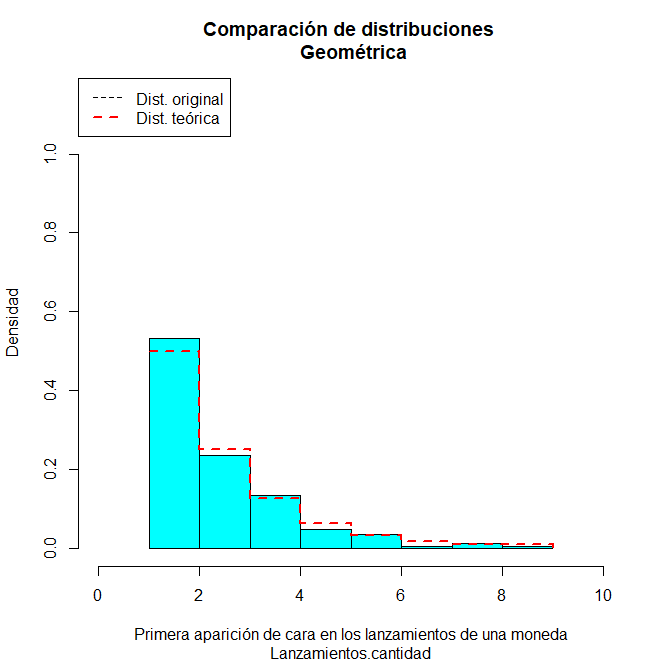
\includegraphics[scale=0.35]{Problema_85.png}
 \end{center}
 El cual coincide con los datos obtenidos,
 que es a lo que se quer\'{\i}a llegar.${}_{\blacksquare}$
\end{solucion}

 \item \begin{enunciado}
 Repita el ejercicio 10.83 con un conjunto nuevo de datos obtenidos
 al llevar a cabo realmente $64$ veces el experimento que se describe.
\end{enunciado}

\begin{solucion}
 Pendiente hasta conseguir una baraja.
\end{solucion}

 \item \begin{enunciado}
 Repita el ejercicio 10.85 con el nuevo conjunto de datos obtenidos
 al realizar $256$ veces el experimento que se describe.
\end{enunciado}

\begin{solucion}
 Pendiente.
\end{solucion}

 \item \begin{enunciado}
 En el ejercicio 1.18 de la p\'agina 28, pruebe la bondad de ajuste
 entre las frecuencias de clase que se observan,
 y las frecuencias esperadas correspondientes de una distribuci\'on normal
 con $\mu = 65$ y $\sigma = 21$.
 Utilice un nivel de significancia de $0.05$.
\end{enunciado}

\begin{solucion}
 La resoluci\'on se har\'a usando ambas pruebas vistas en el libro:
 la prueba de bondad de ajuste $\chi^2$ y la prueba de Geary.
 \begin{datos}
  Usando los datos del ejercicio 1.18, incluyendo el diagrama de tallo y hoja, 
  se tiene lo siguiente:
  \begin{itemize}
   \item Tama\~no de la muestra: $n=60$.
   \item Media muestral: $\bar{x} = \frac{3\,929}{60} = 65.38\bar{3}$.
   \item Varianza muestral:
   $s^2 = \frac{1\,581\,059}{3\,540} \approx 44.6776836158192$
   \item Frecuencia observada individualmente:
   \begin{center}
    \begin{tabular}{ccccccccc}
     $23$ & $60$ & $79$ & $32$ & $57$ & $74$ & $52$ & $70$ & $82$ \\
     $36$ & $80$ & $77$ & $81$ & $95$ & $41$ & $65$ & $92$ & $85$ \\
     $55$ & $76$ & $52$ & $10$ & $64$ & $75$ & $78$ & $25$ & $80$ \\
     $98$ & $81$ & $67$ & $41$ & $71$ & $83$ & $54$ & $64$ & $72$ \\
     $88$ & $62$ & $74$ & $43$ & $60$ & $78$ & $89$ & $76$ & $84$ \\
     $48$ & $84$ & $90$ & $15$ & $79$ & $34$ & $67$ & $17$ & $82$ \\
     $69$ & $74$ & $63$ & $80$ & $85$ & $61$
    \end{tabular}
   \end{center}
   las cuales se pueden agrupar en las $9$ clases que hicieron
   en el diagrama de tallo y hoja del ejercicio al que se hace referencia, 
   lo cual se muestra en la siguiente tabla:
   \begin{center}
    \begin{tabular}{cc}
     \hline 
     \textbf{L\'{\i}mites de clase} & $o_i$ \\
     \hline 
     $ 9.5 - 19.5$ &  $3$ \\
     $19.5 - 29.5$ &  $2$ \\
     $29.5 - 39.5$ &  $3$ \\
     $39.5 - 49.5$ &  $4$ \\
     $49.5 - 59.5$ &  $5$ \\
     $59.5 - 69.5$ & $11$ \\
     $69.5 - 79.5$ & $14$ \\
     $79.5 - 89.5$ & $14$ \\
     $89.5 - 99.5$ &  $4$ \\
     \hline 
    \end{tabular}
   \end{center}
   \item Probabilidades esperadas: usando la tabla A.3,
   se encuentra las \'areas bajo la curva para cada clase como sigue:
   \begin{center}
    \begin{tabular}{cccc}
     \hline 
     \multicolumn{3}{c}{\textbf{L\'{\i}mites de clase}} & $p_i$ \\
     \hline 
     $ 9.5$ & $-$ & $19.5$ &
     $P\left( Z<\frac{19.5 - 65}{21}\right) \approx P(Z<-2.17)\approx 0.0150$ \\
     $19.5$ & $-$ & $29.5$ &
     $P\left( \frac{19.5 - 65}{21} < Z < \frac{29.5 - 65}{21} \right)
     \approx P(Z < -1.69) - P(Z < -2.17)$ \\
     & & & $\approx 0.0455 - 0.0150 = 0.0305$ \\
     $29.5$ & $-$ & $39.5$ &
     $P\left( \frac{29.5 - 65}{21} < Z < \frac{39.5 - 65}{21} \right)
     \approx P(Z < -1.21) - P(Z < -1.69)$ \\
     & & & $\approx 0.1131 - 0.0455 = 0.0676$ \\
     $39.5$ & $-$ & $49.5$ &
     $P\left( \frac{39.5 - 65}{21} < Z < \frac{49.5 - 65}{21} \right)
     \approx P(Z < -0.74) - P(Z < -1.12)$ \\
     & & & $\approx 0.2296 - 0.1131 = 0.1165$ \\
     $49.5$ & $-$ & $59.5$ &
     $P\left( \frac{49.5 - 65}{21} < Z < \frac{59.5 - 65}{21} \right)
     \approx P(Z < -0.26) - P(Z < -0.74)$ \\
     & & & $\approx 0.3974 - 0.2296 = 0.1678$ \\
     $59.5$ & $-$ & $69.5$ &
     $P\left( \frac{59.5 - 65}{21} < Z < \frac{69.5 - 65}{21} \right)
     \approx P(Z < 0.21) - P(Z < -0.26)$ \\
     & & & $\approx 0.5832 - 0.3974 = 0.1858$ \\
     $69.5$ & $-$ & $79.5$ &
     $P\left( \frac{69.5 - 65}{21} < Z < \frac{79.5 - 65}{21} \right)
     \approx P(Z < 0.69) - P(Z < 0.21)$ \\
     & & & $\approx 0.7549 - 0.5832 = 0.1717$ \\
     $79.5$ & $-$ & $89.5$ &
     $P\left( \frac{79.5 - 65}{21} < Z < \frac{89.5 - 65}{21} \right)
     \approx P(Z < 1.17) - P(Z < 0.69)$ \\
     & & & $\approx 0.879 - 0.7549 = 0.1241$ \\
     $89.5$ & $-$ & $99.5$ &
     $P\left( \frac{89.5-65}{21}<Z\right)\approx 1-P(Z < 1.17)\approx 1 - 0.879 = 0.121$ \\
     \hline
    \end{tabular}
   \end{center}
   \item Frecuencias esperadas, determinado por clase
   y considerando el redondeo a un decimal: $E = \left\{
   \left.e_i=n\cdot p_i\,\right|\,\forall i\in\mathbb{N}\cap[1,9] \right\}
   = \{ e_1 = 60\times 0.015 = 0.9, e_2 = 60 \times 0.0305 = 1.8,
   e_3 = 60 \times 0.0676 = 4.1, e_4 = 60 \times 0.1165 = 7,
   e_5 = 60 \times 0.1678 = 10.1, e_6 = 60 \times 0.1858 = 11.1,
   e_7 = 60 \times 0.1717 = 10.3, e_8 = 60 \times 0.1241 = 7.4,
   e_9 = 60 \times 0.121 = 7.3 \}$
  \end{itemize}
  Dado que las pruebas de bondad por m\'etodo de $\chi^2$ no son confiables
  cuando la frecuencia esperada de una celda es menor a $5$,
  se agrupar\'an los datos, como sigue:
  \begin{itemize}
   \item Frecuencias observadas, probabilidades esperadas y frecuencias
   esperadas por clase, se muestran a continuaci\'on en la siguiente tabla:
   \begin{center}
    \begin{tabular}{ccccccc}
     \hline
     \textbf{L\'{\i}mites de clase} & $o_i$ & & $p_i$ & & $e_i$ & \\
     \hline 
     $ 9.5 - 19.5$ &  $3$ &
     \multirow{3}{*}{\hspace{-0.7cm} $\left.
     \begin{matrix}\phantom{0}\\\phantom{0}\\\phantom{0}\end{matrix}
     \right\} 8$}
     & $0.015$ &
     \multirow{3}{*}{\hspace{-0.5cm}$\left.
     \begin{matrix}\phantom{0}\\\phantom{0}\\\phantom{0}\end{matrix}
     \right\} 0.1131$}
     & $0.9$ &
     \multirow{3}{*}{\hspace{-0.7cm} $\left.
     \begin{matrix}\phantom{0}\\\phantom{0}\\\phantom{0}\end{matrix}
     \right\} 6.8$} \\
     $19.5 - 29.5$ &  $2$ &\hspace{-0.7cm}& $0.0305$ &\hspace{-0.5cm}& $1.8$  \\
     $29.5 - 39.5$ &  $3$ &\hspace{-0.7cm}& $0.0676$ &\hspace{-0.5cm}& $4.1$  \\
     $39.5 - 49.5$ &  $4$ &\hspace{-0.7cm}& $0.1165$ &\hspace{-0.5cm}&  $7$   \\
     $49.5 - 59.5$ &  $5$ &\hspace{-0.7cm}& $0.1678$ &\hspace{-0.5cm}& $10.1$ \\
     $59.5 - 69.5$ & $11$ &\hspace{-0.7cm}& $0.1858$ &\hspace{-0.5cm}& $11.1$ \\
     $69.5 - 79.5$ & $14$ &\hspace{-0.7cm}& $0.1717$ &\hspace{-0.5cm}& $10.3$ \\
     $79.5 - 89.5$ & $14$ &\hspace{-0.7cm}& $0.1241$ &\hspace{-0.5cm}& $7.4$  \\
     $89.5 - 99.5$ &  $4$ &\hspace{-0.7cm}&  $0.121$ &\hspace{-0.5cm}& $7.3$  \\
     \hline 
    \end{tabular}
   \end{center}
   \item Celdas totales del experimento: $k=7$.
   \item Grados de libertad de la prueba $\chi^2$: $v= k-1 = 6$.
  \end{itemize}
 \end{datos}
 
 \begin{hipotesis}
  Prueba de bondad de ajuste para probar $H_0:$
  que la variable aleatoria $X$, de la calificaci\'on en el examen final
  para el curso de estad\'{\i}stica elemental,
  sigue una distribuci\'on normal
  con media $\mu=6.5$ y desviaci\'on est\'andar $\sigma = 2.1$,
  contra la alternativa $H_1$ de que no es as\'{\i}.
 \end{hipotesis}

 \begin{significancia}
  $\alpha = 0.05$.
 \end{significancia}

 \begin{region}
  De la tabla A.5, se tiene el valor cr\'{\i}tico
  $\chi^2_{\alpha,v} = \chi^2_{0.05,6} \approx 12.592$,
  por lo que la regi\'on de rechazo est\'a dado
  para $\chi^2 > 12.592$, donde
  $\chi^2 = \sum_{i=1}^{k} \frac{\left( o_i - e_i \right)^2}{e_i}$.
  O bien, de la tabla A.3, se tiene el valor cr\'{\i}tico
  $Z_{\alpha/2} = Z_{0.025} \approx 1.96$,
  por lo que la regi\'on de rechazo tambi\'en est\'a dado
  para $Z < -1.96$ o $Z > 1.96$,
  donde $Z = \frac{U - 1}{0.2661/\sqrt{n}}$ y, a su vez,
  $U = \frac{\sqrt{\pi/2} \sum_{i=1}^{n} \left| X_i - \overline{X} \right|/n}{
  \sqrt{\sum_{i=1}^n \left( X_i - \overline{X} \right)^2/n}}$
 \end{region}

 \begin{estadistico}
  Para la prueba de $\chi^2$, el estad\'{\i}stico est\'a dado por:
  \begin{eqnarray*}
   \chi^2 & = & \sum_{i=1}^{k} \frac{\left( o_i - e_i \right)^2}{e_i} \\
   & \approx & \frac{(8-6.8)^2}{6.8} + \frac{(4-7)^2}{7} +
   \frac{(5-10.1)^2}{10.1} + \frac{(11-11.1)^2}{11.1} + \\
   & & 
   \frac{(14-10.3)^2}{10.3} + \frac{(14-7.4)^2}{7.4} + \frac{(4-7.3)^2}{7.3} \\
   & = & \frac{1.44}{6.8} + \frac{9}{7} + \frac{26.01}{10.1} +
   \frac{0.01}{11.1}+\frac{13.69}{10.3}+\frac{43.56}{7.4}+\frac{10.89}{7.3} \\
   & \approx & 0.2118 + 1.2857 + 2.5752 + 0.0009 + 1.3291 + 5.8865 + 1.4918
   = 12.781
  \end{eqnarray*}
  Mientras que, para la prueba de Geary, el c\'alculo del estad\'{\i}stico
  se realiza como sigue, realizando previamente algunos c\'alculos:
  \par 
  Primero se requieren los valores de $x_i - \bar{x}$, los cuales se
  han calculado en el proceso de obtener la desviaci\'on est\'andar
  durante la soluci\'on del problema 1.18, luego entonces, se tiene que:
  \begin{eqnarray*}
   \sum_{i=1}^{60} \left| x_i - \overline{x} \right| & = &
   \frac{1}{60}\left( |-2549| + |-329| + |811| + |-2009| + |-509| + |511| +
   |-809| + |271| + \right. \\
   & & \phantom{\frac{1}{60}(} |991| + |-1769| + |871| + |691| + |931| +
   |1771| + |-1469| + |-29| + \\
   & & \phantom{\frac{1}{60}(} |1591| + |1171| + |-629| + |631| + |-809| +
   |-3329| + |-89| + |571| + \\
   & & \phantom{\frac{1}{60}(} |751| + |-2429| +  |871| + |1951| + |931| + 
   |91| + |-1469| + |331| +  |1051| + \\
   & & \phantom{\frac{1}{60}(} |-689| + |-89| + |391| + |1351| + 
   |-209| + |511| + |-1349| + |-329| + \\
   & & \phantom{\frac{1}{60}(} |751| + |1411| + |631| + |1111| + |-1049| + 
   |1111| + |1471| + |-3029| + \\
   & & \phantom{\frac{1}{60}(} |811| + |-1889| + |91| + |-2909| + |991| + 
   |211| + |511| + |-149| + |871| + \\
   & & \phantom{\frac{1}{60}(} \left. |1171| + |-269| \right)
   = \frac{60\,370}{60} = \frac{6\,037}{6} = 1\,006.1\bar{6}
  \end{eqnarray*}
  y
  \begin{equation*}
   \sum_{i=1}^{60} \left( x_i - \overline{x} \right)^2 = s^2\times 59 =
   \frac{1\,581\,059}{3\,540} \times 59 = \frac{1\,581\,059}{60}
  \end{equation*}
  Luego entonces
  \begin{eqnarray*}
   U & = & \frac{
   \displaystyle{\sqrt{\pi/2}
   \frac{\sum_{i=1}^n \left| X_i - \overline{X} \right|}{n}}
   }{
   \displaystyle{\sqrt{
   \frac{\sum_{i =1}^n \left( X_i - \overline{X} \right)^2}{n}}}
   } 
   = \frac{\displaystyle{\sqrt{\pi/2} \frac{6\,037}{360}}}{
   \displaystyle{\sqrt{ \frac{1\,581\,059}{3\,600} }}}
   = \frac{\displaystyle{\sqrt{\pi} \frac{6\,037}{\cancelto{6}{360}}}}{
   \displaystyle{ \frac{\sqrt{2 \times 1\,581\,059}}{\cancel{60}} }}
   = \frac{\sqrt{3\,162\,118\pi} 6\,037}{3\,162\,118\times 6} \\
   & = & \frac{6\,037\sqrt{3\,162\,118\pi}}{18\,972\,708}
   \approx 1.00289583
  \end{eqnarray*}
  Por lo que el estad\'{\i}stico $Z$ para la prueba de Geary es:
  \begin{eqnarray*}
   Z & = & \frac{U - 1}{0.2661/\sqrt{n}} = 
   \frac{\displaystyle{\frac{6\,037\sqrt{3\,162\,118\pi}}{18\,972\,708} - 1}
   }{\displaystyle{\frac{0.2661}{\sqrt{60}}}}
   = \frac{\displaystyle{
   \frac{6\,037\sqrt{3\,162\,118\pi} - 18\,972\,708}{18\,972\,708}}}{
   \displaystyle{\frac{2\,661}{10\,000\cdot 2\sqrt{15}}}} \\
   & = & \frac{\cancelto{5\,00}{20\,000}\,\,\,\sqrt{15} \cdot
   \left(6\,037\sqrt{3\,162\,118\pi} - 18\,972\,708\right)}{
   2\,661\cdot \cancelto{4\,743\,177}{18\,972\,708}} \\
   & = & \frac{5\,000\sqrt{15}\left(
   6\,037\sqrt{3\,162\,118\pi}-18\,972\,708\right)}{
   12\,621\,593\,997} \approx 0.084295 \\
  \end{eqnarray*}
 \end{estadistico}

 \begin{decision}
  Se presenta una discrepancia al comparar las pruebas de bondad de $\chi^2$
  y de Geary.
  En la literatura se sugiere que, si existe discrepancia entre dos pruebas,
  se debe tomar una decisi\'on conservadora, es decir,
  se rechaza $H_0$ a favor de $H_1$.
 \end{decision}

 \begin{conclusion}
  Se obtiene evidencia suficiente, por la prueba $\chi^2$, para afirmar
  que las calificaciones en el examen final del curso de estad\'{\i}stica
  elemental no sigue una distribuci\'on normal con media $\mu = 6.5$
  y desviaci\'on est\'andar $\sigma = 2.1$.
 \end{conclusion}
 
 En el c\'odigo registrado en el archivo
 \texttt{P17\_Prueba\_de\_normalidad\_01.r} se realiza este procedimiento.
 El c\'odigo permite modificar los valores iniciales que corresponden a:
 \texttt{datos} que guarda los datos de la lectura de un archivo,
 en este caso se lee el archivo \texttt{BD24\_Problema\_088.csv},
 y este \'ultimo nombre es el que se modifica para leer otros archivos;
 \texttt{varInteres} para indicar el nombre de la columna
 que corresponde a los datos;
 \texttt{media} y \texttt{desv.est} para indicar valores presupuestos
 para la media y la desviaci\'on est\'andar,
 o bien se les puede asignar \texttt{NULL} y se
 estimar\'an los valores;
 \texttt{clases} para indicar con un n\'umero la cantidad de clases
 a considerar o una lista con los n\'umeros m\'aximos y m\'{\i}nimo
 de todas las clases, as\'{\i} como tambi\'en los valores de corte
 que separan cada clase,
 o bien indicar con \texttt{NULL} si se desee crear la divisi\'on de clases
 de forma autom\'atica;
 y \texttt{graficaHist} para indicar, con \texttt{TRUE},
 si se desea realizar una gr\'afica de comparaci\'on entre la distribuci\'on
 normal supuesta y la distribuci\'on de la muestra en un histograma,
 o \texttt{FALSE} en caso contrario.
 \par
 El programa espera al menos los datos correspondientes a la base de datos,
 escrito en un arhivo \texttt{.csv} con una columna con los datos, 
 identificado por \texttt{varInteres}.
 \par
 El programa realiza los c\'alculos de bondad de ajuste correspondientes
 a los m\'etodos vistos en el libro, es decir, por el m\'etodo $\chi^2$,
 considerado tambi\'en como m\'etodo de Pearson,
 y el m\'etodo de Geary.
 Adem\'as de estos m\'etodos, se calculas los estad\'{\i}sticos
 correspondientes a las pruebas de Kolmogorov-Smirnov, el de Lilliefors,
 que es una versi\'on mejorada del de Kolmogorov-Smirnov (K-S)
 para las pruebas de normalidad y el de Shapiro-Wilk.
 Adem\'as de los estad\'{\i}sticos, se calculan los $p-$valores de estos.
 Aunque tienen sus respectivas diferencias, se hace notar aqu\'{\i}
 algunas de ellas:
 el m\'etodo $\chi^2$ y el de Kolmogorov-Smirnov son los \'unicos
 m\'etodos que usan las supociones de los par\'amtros poblaciones hechas mientras que el resto de m\'etodos usan siempre estimaciones
 a partir de los datos independientemente de que existan supociones previas;
 por otro lado, los m\'etodos de bondad de ajuste $\chi^2$ y K-S
 son gen\'ericos, mientras que el resto sirven para pruebas de normalidad
 en espec\'{\i}fico.
 Cabe hacer notar que en este programa no se indicar\'an regiones de rechazo, 
 ya que no se encuentran en algunos de estos m\'etodos los procesos inversos
 para calcular una regi\'on de rechazo a partir de un valor de probabilidad.
 Finalmente, cabe mencionar que se usar\'an los paquetes \texttt{MASS}
 y \texttt{nortest} para los gr\'aficos y para la prueba de Lilliefors,
 respectivamente.
 \par
 El programa siempre mostrar\'a en su salida lo siguiente:
 \texttt{nombres} que contiene el nombre de la variable de los datos;
 \texttt{n} para el tama\~no muestral usado;
 \texttt{X de chi2} que indica el estad\'{\i}stico $\chi^2$
 del m\'etodo $\chi^2$ de Pearson;
 \texttt{param chi2} que indica la cantidad de grados de libertad
 usado durante el m\'etodo de $\chi^2$;
 \texttt{Valor-p chi2} para indicar el $p-$valor calculado
 durante el m\'etodo de $\chi^2$;
 \texttt{Z de Geary} con el valor del estad\'{\i}stico $Z$
 calculado con la prueba de Geary;
 \texttt{Valor-p Geary} para indicar el $p-$valor calculado
 durante la prueba de Geary;
 \texttt{D de K-S} con el valor del estad\'{\i}stico $D$
 calculado con la prueba de Kolmogorov-Smirnov;
 \texttt{Valor-p K-S} para indicar el $p-$valor calculado
 con el estad\'{\i}stico $D$ de Kolmogorov-Smirnov;
 \texttt{D de K-S Lilliefors} con el valor del estad\'{\i}stico $D$
 calculado con la prueba de Lilliefors-Kolmogorov-Smirnov;
 \texttt{Valor-p K-S Lilliefors} para indicar el $p-$valor calculado
 con el estad\'{\i}stico $D$ de Lilliefors-Kolmogorov-Smirnov;
 \texttt{W de Shapiro} con el valor del estad\'{\i}stico $W$
 calculado con la prueba de Shapiro-Wilk;
 y, finalmente, \texttt{valor-p Shapiro} para indicar el $p-$valor calculado
 durante la prueba de Shapiro-Wilk.
 El c\'odigo junto con el resultado se muestra a continuaci\'on:
 \begin{verbatim}
> require(MASS)
> require(nortest)
> datos<-read.csv("DB24_Problema_088.csv",sep=";",encoding="UTF-8")
> varInteres<-"Calificación"
> media<-65
> desv.est<-21
> clases<-c(9.5,19.5,29.5,39.5,49.5,59.5,69.5,79.5,89.5,99.5)
> graficaHist<-TRUE
> colapsar<-function(p1,f1,lim1=5){
+   np1<-p1
+   nf1<-f1
+   tocollapse<-which((p1*sum(f1))<lim1)
+   while(length(tocollapse)>0){
+     x<-tocollapse[1]
+     if (x<(length(f1)/2)){
+       np1[x+1]<-p1[x]+p1[x+1]
+       nf1[x+1]<-f1[x]+f1[x+1]
+     }else{
+       np1[x-1]<-p1[x]+p1[x-1]
+       nf1[x-1]<-f1[x]+f1[x-1]
+     }
+     p1<-np1[-x]
+     f1<-nf1[-x]
+     np1<-p1
+     nf1<-f1
+     tocollapse<-which((p1*sum(f1))<lim1)
+   }
+   return(list(probs=p1,freqs=f1))  
+ }
> calculos2<-function(x,media=NULL,desv.est=NULL,clases){
+   n<-length(x)
+   ajuste<-0
+   if (is.null(media)) {
+     media<-mean(x)
+     ajuste<-ajuste+1
+   }
+   if (is.null(desv.est)) {
+     desv.est<-sd(x)
+     ajuste<-ajuste+1
+   }
+   if(is.null(clases)){
+     k<-round(sqrt(length(x)),0)
+     clases<-min(x)
+     clases<-c(clases,diff(range(x))/k*(1:(k-1))+min(x))
+     clases<-c(clases,max(x))
+   }
+   if(length(clases)==1){
+     k<-clases[1]
+     clases<-min(x)
+     clases<-c(clases,diff(range(x))/k*(1:(k-1))+min(x))
+     clases<-c(clases,max(x))
+   }
+   k<-length(clases)
+   frecObs<-hist(x,clases)$count
+   probEsp<-pnorm(clases[2],media,desv.est)
+   if(k>3) for(i in (2:(k-2))) {
+     probEsp<-c(probEsp,
+                pnorm(clases[i+1],media,desv.est,lower.tail=TRUE)
+                -pnorm(clases[i],media,desv.est,lower.tail=TRUE))
+   }
+   probEsp<-c(probEsp,1-sum(probEsp))
+   U<-sqrt(pi/2)*mean(abs(x-mean(x)))/sqrt(var(x)*(n-1)/n)
+   Geary.statistic<-(U-1)/(0.2661/sqrt(n))
+   Geary.p.value<-2*pnorm(abs(Geary.statistic),lower.tail=FALSE)
+   pruebaKSlillie<-lillie.test(x)
+   pruebaSW<-shapiro.test(x)
+   pruebaks<-ks.test(x[!duplicated(x)],"pnorm",mean=media,sd=desv.est)
+   ajuste<-0
+   r1<-colapsar(probEsp,frecObs)
+   frecObsC<-r1$freqs
+   probEspC<-r1$probs
+   if(length(frecObsC)>1){
+     pruebachisq<-chisq.test(frecObsC,p=probEspC)
+   }else{
+     pruebachisq<-NA
+   }
+   r<-c(n, pruebachisq$statistic, pruebachisq$parameter-ajuste,
+        pruebachisq$p.value, Geary.statistic, Geary.p.value,
+        pruebaks$statistic, pruebaks$p.value, pruebaKSlillie$statistic,
+        pruebaKSlillie$p.value, pruebaSW$statistic, pruebaSW$p.value)
+   return(r)
+ } 
> generaGrafica<-function(x,media,desv.est,clases,nombres){
+   if (is.null(media)) {
+     media<-mean(x)
+   }
+   if (is.null(desv.est)) {
+     desv.est<-sd(x)
+   }
+   if(is.null(clases)){
+     ni<-round(sqrt(length(x)),0)
+   }else if(length(clases)==1){
+     ni<-clases[1]
+   } else ni<-length(clases)
+   x11()
+   truehist(x,nbins=ni,sub=nombres,xlab="")
+   x<-seq(min(x)*.8,max(x)*1.2,l=100)
+   lines(x,dnorm(x,mean=media,sd=desv.est),lwd=1.5)
+ }
> valores<-datos[,varInteres]
> valores<-valores[!is.na(valores)]
> if(length(valores)<3){
+   stop("Se necesita de al menos 3 valores para proceder")
+ }
> r1<-t(as.matrix(calculos2(valores,media,desv.est,clases)))
> r1<-data.frame(nombre=varInteres,r1)
> names(r1)<-c("nombres","n","X de chi2", "param chi2", "Valor-p chi2",
+              "Z de Geary", "Valor-p Geary", "D de K-S", "Valor-p K-S",
+              "D de K-S Lilliefors", "Valor-p K-S Lilliefors",
+              "W de Shapiro","Valor-p Shapiro")
> r1
       nombres  n X de chi2 param chi2 Valor-p chi2 Z de Geary Valor-p Geary
1 Calificación 60  12.86244          6   0.04527318 0.08429539     0.9328216
    D de K-S Valor-p K-S D de K-S Lilliefors Valor-p K-S Lilliefors W de Shapiro
1 0.09817138   0.7534067           0.1398566            0.005196948    0.9176965
  Valor-p Shapiro
1    0.0006202501
> if (graficaHist){
+   generaGrafica(valores,media,desv.est,clases,varInteres)
+ }
 \end{verbatim}
 \vspace{-0.5cm}
 que incluye la siguiente figura:
 \begin{center}
  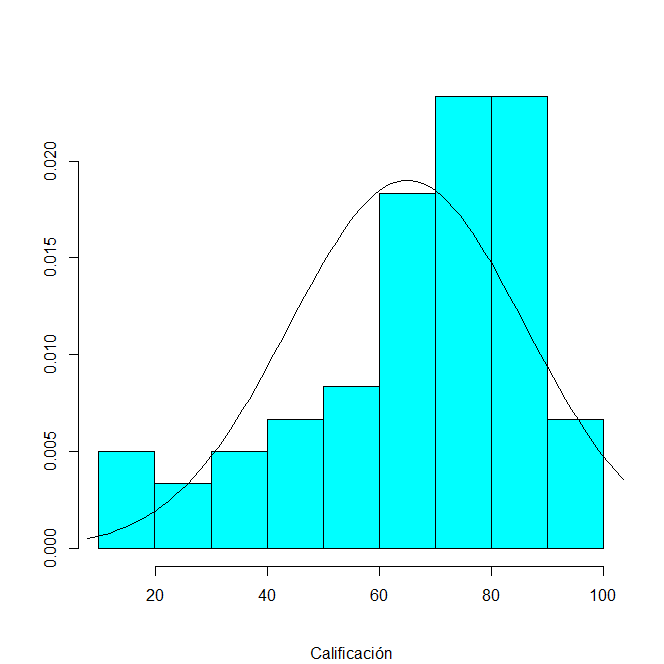
\includegraphics[scale=0.35]{Problema_88.png}
 \end{center}
 Lo cual coincide con los obtenido en las pruebas $\chi^2$ y de Geary.
 En el caso de la prueba $\chi^2$ hay una ligera discrepancia
 debido a los redondeos a un decimal.
 Adem\'as, se pueden observar c\'omo se obtiene valores de otras pruebas.
 En el caso de las pruebas K-S y Lilliefors, se requiere que no haya valores
 duplicados, por lo que podr\'{\i}a dudarse de su resultado,
 adem\'as de que su uso es recomendable para muestras grandes, mayores a $100$;
 por otro lado, la prueba de Shapiro-Wilk es bueno para meustras peque\~nas
 aunque sus ajuste es a par\'ametros estimados $\bar{x}$ y $s^2$.
 Luego entonces, se toma mayor fuerza en la prueba $\chi^2$,
 la cual ya indica que no hay un buen ajuste a una poblaci\'on normal,
 que es a lo que se quer\'{\i}a llegar.${}_{\blacksquare}$
\end{solucion}

 \item \begin{enunciado}
 En el ejercicio 1.19 de la p\'agina 28, pruebe la bondad de ajuste
 entre las frecuencias de clase que se observan
 y las frecuencias esperadas correspondientes de una distribuci\'on normal
 con $\mu = 1.8$ y $\sigma = 0.4$.
 Utilice un nivel de significancia de $0.01$.
\end{enunciado}

\begin{solucion}
 La resoluci\'on se har\'a usando ambas pruebas vistas en el libro:
 la prueba de bondad de ajuste $\chi^2$ y la prueba de Geary.
 \begin{datos}
  Usando los datos del ejercicio 1.19, incluyendo el diagrama de tallo y hoja, 
  se tiene lo siguiente:
  \begin{itemize}
   \item Tama\~no de la muestra: $n=30$.
   \item Media muestral: $\bar{x} = \frac{829}{300} = 2.79\bar{6}$.
   \item Varianza muestral:
   $s^2 = \frac{431\,609}{87\,000} \approx 4.96102$
   \item Frecuencia observada individualmente:
   \begin{center}
    \begin{tabular}{cccccc}
     $2.0$ & $3.0$ & $0.3$ & $3.3$ & $1.3$ & $0.4$ \\
     $0.2$ & $6.0$ & $5.5$ & $6.5$ & $0.2$ & $2.3$ \\
     $1.5$ & $4.0$ & $5.9$ & $1.8$ & $4.7$ & $0.7$ \\
     $4.5$ & $0.3$ & $1.5$ & $0.5$ & $2.5$ & $5.0$ \\
     $1.0$ & $6.0$ & $5.6$ & $6.0$ & $1.2$ & $0.2$ 
    \end{tabular}
   \end{center}
   las cuales se pueden agrupar en las $7$ clases que hicieron
   en el diagrama de tallo y hoja del ejercicio al que se hace referencia, 
   lo cual se muestra en la siguiente tabla:
   \begin{center}
    \begin{tabular}{cc}
     \hline 
     \textbf{L\'{\i}mites de clase} & $o_i$ \\
     \hline 
     $-0.05 - 0.95$ &  $8$ \\
     $0.95 - 1.95$ & $6$ \\
     $1.95 - 2.95$ & $3$ \\
     $2.95 - 3.95$ & $2$ \\
     $3.95 - 4.95$ & $3$ \\
     $4.95 - 5.95$ & $4$ \\
     $5.95 - 6.95$ & $4$ \\
     \hline 
    \end{tabular}
   \end{center}
   \item Probabilidades esperadas: usando la tabla A.3,
   se encuentra las \'areas bajo la curva para cada clase como sigue:
   \begin{center}
    \begin{tabular}{cccc}
     \hline 
     \multicolumn{3}{c}{\textbf{L\'{\i}mites de clase}} & $p_i$ \\
     \hline 
     $-0.05$ & $-$ & $0.95$ &
     $P\left( Z<\frac{0.95 - 1.8}{0.4}\right) \approx P(Z<-2.125)\approx 0.0168$ \\
     $0.95$ & $-$ & $1.95$ &
     $P\left( \frac{0.95 - 1.8}{0.4} < Z < \frac{1.95 - 1.8}{0.4} \right)
     \approx P(Z < 0.375) - P(Z < -2.125)$ \\
     & & & $\approx 0.6461 - 0.0168 = 0.6293$ \\
     $1.95$ & $-$ & $2.95$ &
     $P\left( \frac{1.95 - 1.8}{0.4} < Z < \frac{2.95 - 1.8}{0.4} \right)
     \approx P(Z < 2.875) - P(Z < 0.375)$ \\
     & & & $\approx 0.998 - 0.6461 = 0.3519$ \\
     $2.95$ & $-$ & $3.95$ &
     $P\left( \frac{2.95 - 1.8}{0.4} < Z < \frac{3.95 - 1.8}{0.4} \right)
     \approx P(Z < 5.375) - P(Z < 2.875)$ \\
     & & & $\approx 1 - 0.998 = 0.002$ \\
     $3.95$ & $-$ & $4.95$ &
     $P\left( \frac{3.95 - 1.8}{0.4} < Z < \frac{4.95 - 1.8}{0.4} \right)
     \approx P(Z < 7.875) - P(Z < 5.375)$ \\
     & & & $\approx 1 - 1 = 0$ \\
     $4.95$ & $-$ & $5.95$ &
     $P\left( \frac{4.95 - 1.8}{0.4} < Z < \frac{5.95 - 1.8}{0.4} \right)
     \approx P(Z < 10.375) - P(Z < 7.875)$ \\
     & & & $\approx 1 - 1 = 0$ \\
     $5.95$ & $-$ & $6.95$ &
     $P\left( Z > \frac{5.95 - 1.8}{0.4} \right) \approx 1 - P(Z < 10.375)$ \\
     & & & $\approx 1 - 1 = 0$ \\
     \hline
    \end{tabular}
   \end{center}
   \item Frecuencias esperadas, determinado por clase
   y considerando el redondeo a un decimal: $E = \left\{
   \left.e_i=n\cdot p_i\,\right|\,\forall i\in\mathbb{N}\cap[1,7] \right\}
   = \{ e_1 = 30\times 0.0168 = 0.5, e_2 = 30 \times 0.6292 = 18.9,
   e_3 = 30 \times 0.3519 = 10.6, e_4 = 30 \times 0.0002 = 0,
   e_5 = 30 \times 0 = 0, e_6 = 30 \times 0 = 0,
   e_7 = 30 \times 0 = 0 \}$
  \end{itemize}
  Dado que las pruebas de bondad por m\'etodo de $\chi^2$ no son confiables
  cuando la frecuencia esperada de una celda es menor a $5$,
  se agrupar\'an los datos, como sigue:
  \begin{itemize}
   \item Frecuencias observadas, probabilidades esperadas y frecuencias
   esperadas por clase, se muestran a continuaci\'on en la siguiente tabla:
   \begin{center}
    \begin{tabular}{ccccccc}
     \hline
     \textbf{L\'{\i}mites de clase} & $o_i$ & & $p_i$ & & $e_i$ & \\
     \hline 
     $-0.05 - 0.95$ &  $8$ &
     \multirow{2}{*}{\hspace{-0.7cm} $\left.
     \begin{matrix} \phantom{0} \\ \phantom{0} \end{matrix}
     \right\} 14$}
     & $0.0168$ &
     \multirow{2}{*}{\hspace{-0.5cm}$\left.
     \begin{matrix} \phantom{0} \\ \phantom{0} \end{matrix}
     \right\} 0.646$}
     & $0.5$ &
     \multirow{2}{*}{\hspace{-0.7cm} $\left.
     \begin{matrix} \phantom{0} \\ \phantom{0} \end{matrix}
     \right\} 19.4$} \\
     $0.95 - 1.95$ & $6$ &\hspace{-0.7cm}& $0.6292$ &\hspace{-0.5cm}& $18.9$  \\
     $1.95 - 2.95$ & $3$ &
     \multirow{5}{*}{\hspace{-0.7cm} $\left.
     \begin{matrix} \phantom{0} \\ \phantom{0} \\ \phantom{0}
     \\\phantom{0} \\ \phantom{0} \end{matrix}
     \right\} 16$}
     & $0.3519$ &
     \multirow{5}{*}{\hspace{-0.5cm}$\left.
     \begin{matrix} \phantom{0} \\ \phantom{0} \\ \phantom{0}
     \\\phantom{0} \\ \phantom{0} \end{matrix}
     \right\} 0.3521$}
     & $10.6$ &
     \multirow{5}{*}{\hspace{-0.7cm} $\left.
     \begin{matrix} \phantom{0} \\ \phantom{0} \\ \phantom{0}
     \\\phantom{0} \\ \phantom{0} \end{matrix}
     \right\} 10.6$} \\     
     $2.95 - 3.95$ & $2$ &\hspace{-0.7cm}& $0.0002$ &\hspace{-0.5cm}& $0$ \\
     $3.95 - 4.95$ & $3$ &\hspace{-0.7cm}& $0$ &\hspace{-0.5cm}& $0$ \\
     $4.95 - 5.95$ & $4$ &\hspace{-0.7cm}& $0$ &\hspace{-0.5cm}& $0$ \\
     $5.95 - 6.95$ & $4$ &\hspace{-0.7cm}& $0$ &\hspace{-0.5cm}& $0$ \\
     \hline 
    \end{tabular}
   \end{center}
   \item Celdas totales del experimento: $k=2$.
   \item Grados de libertad de la prueba $\chi^2$: $v= k-1 = 1$.
  \end{itemize}
 \end{datos}
 
 \begin{hipotesis}
  Prueba de bondad de ajuste para probar $H_0:$
  que la variable aleatoria $X$, de los a\~nos de vida de las bombas
  de combustible de cierto tipo, sigue una distribuci\'on normal
  con media $\mu=1.8$ y desviaci\'on est\'andar $\sigma = 0.4$,
  contra la alternativa $H_1$ de que no es as\'{\i}.
 \end{hipotesis}

 \begin{significancia}
  $\alpha = 0.01$.
 \end{significancia}

 \begin{region}
  De la tabla A.5, se tiene el valor cr\'{\i}tico
  $\chi^2_{\alpha,v} = \chi^2_{0.01,1} \approx 6.635$,
  por lo que la regi\'on de rechazo est\'a dado
  para $\chi^2 > 6.635$, donde
  $\chi^2 = \sum_{i=1}^{k} \frac{\left( o_i - e_i \right)^2}{e_i}$.
  O bien, de la tabla A.3, se tiene el valor cr\'{\i}tico
  $Z_{\alpha/2} = Z_{0.005} \approx 2.575$,
  por lo que la regi\'on de rechazo tambi\'en est\'a dado
  para $Z < -2.575$ o $Z > 2.575$,
  donde $Z = \frac{U - 1}{0.2661/\sqrt{n}}$ y, a su vez,
  $U = \frac{\sqrt{\pi/2} \sum_{i=1}^{n} \left| X_i - \overline{X} \right|/n}{
  \sqrt{\sum_{i=1}^n \left( X_i - \overline{X} \right)^2/n}}$
 \end{region}

 \begin{estadistico}
  Para la prueba de $\chi^2$, el estad\'{\i}stico est\'a dado por:
  \begin{eqnarray*}
   \chi^2 & = & \sum_{i=1}^{k} \frac{\left( o_i - e_i \right)^2}{e_i} \\
   & \approx & \frac{(14-19.4)^2}{19.4} + \frac{(16-10.6)^2}{10.6} \\
   & = & \frac{(-5.4)^2}{19.4} + \frac{5.4^2}{10.6}
   = \frac{29.16(53) + 29.16(97)}{1\,028.2}
   = \frac{4\,374}{1\,028.2} \\
   & = & \frac{21\,870}{5\,141} \approx 4.254
  \end{eqnarray*}
  Mientras que, para la prueba de Geary, el c\'alculo del estad\'{\i}stico
  se realiza como sigue, realizando previamente algunos c\'alculos:
  \par 
  Primero se requieren los valores de $x_i - \bar{x}$, los cuales se
  han calculado en el proceso de obtener la desviaci\'on est\'andar
  durante la soluci\'on del problema 1.19, luego entonces, se tiene que:
  \begin{eqnarray*}
   \sum_{i=1}^{60} \left| x_i - \overline{x} \right| & = &
   \frac{1}{30}\left( |-23.9| + |6.1| + |-74.9| + |15.1| + |-44.9| + |-71.9| +
   |-77.9| + \right. \\
   & & \phantom{\frac{1}{60}(}  |96.1| + |81.1| + |111.1| + |-77.9| + |-14.9| +
   |-38.9| + |36.1| + |93.1| + \\
   & & \phantom{\frac{1}{60}(} |-29.9| + |57.1| + |-62.9| + |51.1| + |-74.9| +
   |-38.9| + |68.9| + \\
   & & \phantom{\frac{1}{60}} \left. |-8.9| + |66.1| + |-53.9| + |96.1| + 
   |84.1| + |96.1| + |-47.9| + |-77.9| \right) \\
   & = & \frac{1\,778.6}{30} = \frac{8\,893}{150} = 59.28\bar{6}
  \end{eqnarray*}
  y
  \begin{equation*}
   \sum_{i=1}^{60} \left( x_i - \overline{x} \right)^2 = s^2\times 29 =
   \frac{431\,609}{\cancelto{3\,000}{87\,000}}\hspace{0.7cm}\times \cancel{29}
   = \frac{431\,609}{3\,000} = 143.869\bar{6}
  \end{equation*}
  Luego entonces
  \begin{eqnarray*}
   U & = & \frac{
   \displaystyle{\sqrt{\pi/2}
   \frac{\sum_{i=1}^n \left| X_i - \overline{X} \right|}{n}}
   }{
   \displaystyle{\sqrt{
   \frac{\sum_{i =1}^n \left( X_i - \overline{X} \right)^2}{n}}}
   } 
   = \frac{\displaystyle{\sqrt{\pi/2} \frac{8\,893}{4\,500}}}{
   \displaystyle{\sqrt{ \frac{431\,609}{90\,000} }}}
   = \frac{\displaystyle{\sqrt{\pi} \frac{8\,893}{\cancelto{15}{4\,500}}}}{
   \displaystyle{
   \frac{\sqrt{2\times 431\,609}}{\cancel{300}} 
   }}
   = \frac{\sqrt{863\,218\pi} 8\,893}{863\,218 \times 15} \\
   & = & \frac{\sqrt{863\,218\pi} 8\,893}{12\,948\,270}
   \approx 1.13102
  \end{eqnarray*}
  Por lo que el estad\'{\i}stico $Z$ para la prueba de Geary es:
  \begin{eqnarray*}
   Z & = & \frac{U - 1}{0.2661/\sqrt{n}} = 
   \frac{\displaystyle{\frac{\sqrt{863\,218\pi} 8\,893}{12\,948\,270} - 1}
   }{\displaystyle{\frac{0.2661}{\sqrt{30}}}}
   = \frac{\displaystyle{
   \frac{\sqrt{863\,218\pi} 8\,893 - 12\,948\,270}{12\,948\,270}}}{
   \displaystyle{\frac{2\,661}{10\,000\cdot \sqrt{30}}}} \\
   & = & \frac{\cancelto{1\,000}{10\,000}\,\,\,\sqrt{30} \cdot
   \left(\sqrt{863\,218\pi} 8\,893 - 12\,948\,270\right)}{
   2\,661\cdot \cancelto{1\,294\,827}{12\,948\,270}} \\
   & = & \frac{1\,000\sqrt{30} \cdot
   \left(\sqrt{863\,218\pi} 8\,893 - 12\,948\,270\right)}{
   3\,445\,534\,647} \approx 2.6969 \\
  \end{eqnarray*}
 \end{estadistico}

 \begin{decision}
  Se presenta una discrepancia al comparar las pruebas de bondad de $\chi^2$
  y de Geary.
  En la literatura se sugiere que, si existe discrepancia entre dos pruebas,
  se debe tomar una decisi\'on conservadora, es decir,
  se rechaza $H_0$ a favor de $H_1$.
 \end{decision}

 \begin{conclusion}
  Se obtiene evidencia suficiente, por la prueba de Geary, para afirmar
  que los a\~nos de vida de las bombas de combustible similares analizados
  no sigue una distribuci\'on normal con media $\mu = 1.8$
  y desviaci\'on est\'andar $\sigma = 0.4$.
 \end{conclusion}

 Finalmente, usando el archivo anexo
 \texttt{P17\_Prueba\_de\_normalidad\_01.r},
 que a su vez requiere los datos del archivo \texttt{BD25\_Problema\_089.csv},
 con los siguientes cambios:
 \begin{verbatim}
> datos<-read.csv("DB25_Problema_089.csv",sep=";",encoding="UTF-8")
> varInteres<-"Duración.años"
> media<-1.8
> desv.est<-0.4
> clases<-c(-0.05,0.95,1.95,2.95,3.95,4.95,5.95,6.95)
> graficaHist<-TRUE
 \end{verbatim}
 \vspace{-0.5cm}
 el programa de R lanza el siguiente resultado:
 \begin{verbatim}
        nombres  n X de chi2 param chi2 Valor-p chi2 Z de Geary Valor-p Geary
1 Duración.años 30  4.227889          1   0.03976487   2.696906   0.006998705
   D de K-S Valor-p K-S D de K-S Lilliefors Valor-p K-S Lilliefors W de Shapiro
1 0.4599408 3.64055e-05            0.153104             0.07061746    0.8789531
  Valor-p Shapiro
1     0.002667603
 \end{verbatim}
 \vspace{-0.5cm}
 que incluye la siguiente figura:
 \begin{center}
  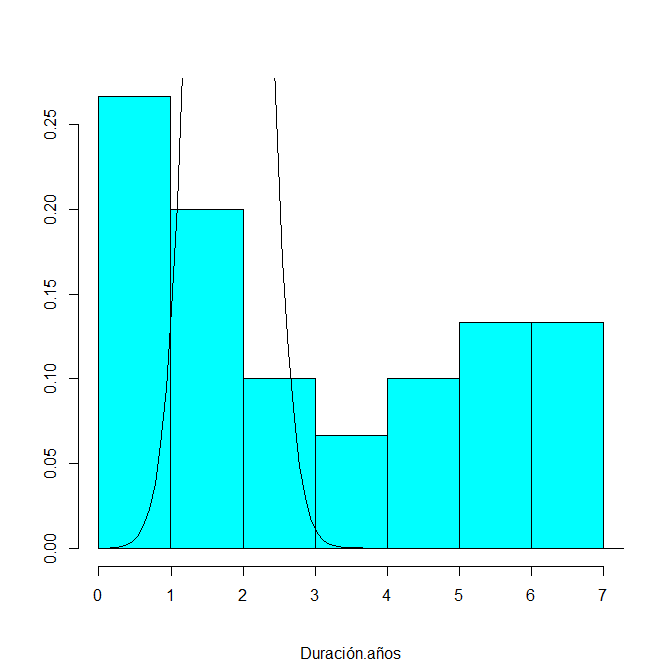
\includegraphics[scale=0.35]{Problema_89.png}
 \end{center}
 Lo cual coincide con los resultado obtenidos.
 Se hace notar que los resultados usando las pruebas K-S y Lilliefors
 requieren de tama\~nos grandes de muestra, mayores a 100,
 por lo que no se toma en cuenta.
 Por otro lado, la prueba de Shapiro, aunque da buenos resultados
 en pruebas peque\~nas como esta, no se est\'a considerando los par\'ametros
 supuestos, como es el caso de la prueba Geary.
 En este caso, parecer\'{\i}a que la \'unica que tiene validez suficiente
 es la prueba $\chi^2$, pero,
 tomando en cuenta de que los par\'ametros estimados para la media y varianza
 son las m\'as probables en las pruebas de Shapiro-Wilk y de Geary,
 entonces se pueden tomar en cuenta como pruebas
 generales para saber si se est\'a distribuyendo a la normal m\'as probable,
 lo cual todo indica que no,
 mientras que la prueba $\chi^2$ de Pearson arroja un valor $P$ muy bajo.
 Entonces, por la direcci\'on a la que se est\'a llevando estas observaciones,
 es razonable llegar a que ciertamente es poco probable
 que la poblaci\'on de la que viene la muestra se distribuya normalmente.
 Finalmente, existe una diferencia entre el valor del estad\'{\i}stico
 $\chi^2$ que se muestra en las soluciones del libro
 con el que se muestra en esta soluci\'on.
 Esto se debe a c\'omo se consideraron las clases,
 de una forma m\'as conservadora,
 y se puede revisar que coincide mejor el resultado
 si se modifica la siguiente l\'{\i}nea en el programa:
 \begin{verbatim}
> clases<-c(0,1,2,3,4,5,6,7)
 \end{verbatim}
 \vspace{-0.5cm}
 lo cual arroja como valor del estad\'{\i}stico el n\'umero
 \texttt{5.154801};
 tambi\'en se muestra una decisi\'on distinta en la soluci\'on del libro,
 lo cual se debe a que \'unicamente se considera la prueba $\chi^2$
 en el libro, lo cual puede ser insuficiente
 al comparar con otras pruebas como se hizo en esta soluci\'on.
 Que es a lo que se quer\'{\i}a llegar.${}_{\blacksquare}$
\end{solucion}

 \item \begin{enunciado}
 Se llev\'o a cabo un estudio en el Instituto Polit\'ecnico y Universidad Estatal de Virginia para determinar si el fuego se puede utilizar como una herramienta de control viable, para aumentar la cantidad de forraje disponible para los venados, durante los meses cr\'{\i}ticos a finales del invierno y principios de la primavera. El calcio es un elemento que requieren las plantas y los animales. La cantidad que la planta toma y almacena est\'a estrechamente correlacionada con la cantidad presente en el suelo. Se formul\'o la hip\'otesis de que el fuego puede cambiar los niveles de calcio presentes en el suelo y afectar as\'{\i} la cantidad disponible para los venados. Se seleccion\'o una extensi\'on grande de tierra en el Fishburn Forest para efectuar un incendio controlado. Se tomaron muestras de suelo de $12$ parcelas de igual \'area justo antes de la quema, y se analizaron para verificar el contenido de calcio. Los niveles de calcio despu\'es de la quema se analizaron en las mismas parcelas. Tales valores, en kilogramos por parcela, se presentan en la siguiente tabla:
 \begin{center}
  \begin{tabular}{ccc}
   & \multicolumn{2}{c}{\hspace{-0.5cm} \textbf{Nivel de calcio (kg/parcela)}} \\
   & \textbf{Antes de} & \textbf{Despu\'es de} \\
   \textbf{Parcela} & \textbf{la quema} & \textbf{la quema} \\
   \hline 
   $\phantom{1}1$ & $50$ &  $\phantom{1}9$ \\
   $\phantom{1}2$ & $50$ & $18$ \\
   $\phantom{1}3$ & $82$ & $45$ \\
   $\phantom{1}4$ & $64$ & $18$ \\
   $\phantom{1}5$ & $82$ & $18$ \\
   $\phantom{1}6$ & $73$ & $\phantom{1}9$ \\
   $\phantom{1}7$ & $77$ & $32$ \\
   $\phantom{1}8$ & $54$ & $\phantom{1}9$ \\
   $\phantom{1}9$ & $23$ & $18$ \\
   $10$ & $45$ & $\phantom{1}9$ \\
   $11$ & $36$ & $\phantom{1}9$ \\
   $12$ & $54$ & $\phantom{1}9$ \\
  \end{tabular}
 \end{center}
 Construya un intervalo de confianza de $95\%$ para la diferencia media en el nivel de calcio presente en el suelo antes y despu\'es del incendio controlado. Suponga que la distribuci\'on de las diferencias en los niveles de calcio es aproximadamente normal.
\end{enunciado}

\begin{solucion}
 Sean $X_1$ y $X_2$ las variables aleatorias de los niveles de calcio, medidos en kilogramos por parcela, antes y despu\'es de la quema, respectivamente, entonces, del enunciado, se tiene el siguiente resumen de datos:
 \begin{itemize}
  \item $X_i \sim n\left( \mu_i, \sigma_i \right)$, para cada $i \in \{ 1,2 \}$.
  \item $\mu_i$ y $\sigma_i$ desconocidos, para cada $i \in \{ 1, 2 \}$.
  \item $n_1 = n_2 = 12$.
  \item $\alpha = 0.05$
 \end{itemize}
 Adem\'as de los datos obtenidos en las $12$ parcelas, antes y despu\'es de la quema, cuyas diferencias en kilogramos por parcela, $D_i = X_1 - X_2$, son:
 \begin{center}
  \begin{tabular}{cccc}
   & \multicolumn{2}{c}{\hspace{-0.5cm} \textbf{Nivel de calcio (kg/parcela)}} \\
   & \textbf{Antes de} & \textbf{Despu\'es de} \\
   \textbf{Parcela} & \textbf{la quema} & \textbf{la quema} & $d_i$ \\
   \hline 
   $\phantom{1}1$ & $50$ &  $\phantom{1}9$ & $41$ \\
   $\phantom{1}2$ & $50$ & $18$ & $32$ \\
   $\phantom{1}3$ & $82$ & $45$ & $37$ \\
   $\phantom{1}4$ & $64$ & $18$ & $46$ \\
   $\phantom{1}5$ & $82$ & $18$ & $64$ \\
   $\phantom{1}6$ & $73$ & $\phantom{1}9$ & $64$ \\
   $\phantom{1}7$ & $77$ & $32$ & $45$ \\
   $\phantom{1}8$ & $54$ & $\phantom{1}9$ & $45$ \\
   $\phantom{1}9$ & $23$ & $18$ & $\phantom{4}5$ \\
   $10$ & $45$ & $\phantom{1}9$ & $36$ \\
   $11$ & $36$ & $\phantom{1}9$ & $27$ \\
   $12$ & $54$ & $\phantom{1}9$ & $45$
  \end{tabular}
 \end{center}
 A partir de estos datos, se puede calcular la media y la desviaci\'on est\'andar de las observaciones pareadas, como se muestra a continuaci\'on. La media muestral se calcula como sigue:
 \begin{equation*}
  \bar{d} = \frac{41 + 32 + 37 + 46 + 64 + 64 + 45 + 45 + 5 + 36 + 27 + 45}{12} = \frac{487}{12} = 40.58\overline{3}
 \end{equation*}
 por lo que la varianza muestral se obtiene, usando el Teorema 8.1, como sigue:
 \begin{eqnarray*}
  s_d^2 & = & \frac{1}{n(n-1)} \left[ n \sum_{i=1}^n d_i^2 - \left( \sum_{i=1}^n d_i \right)^2 \right] \\
  & = & \frac{12\left( 41^2 + 32^2 + 37^2 + 46^2 + 64^2 + 64^2 + 45^2 + 45^2 + 5^2 + 36^2 + 27^2 + 45^2 \right) - 487^2}{12(11)} \\
  & = & \frac{12\left( 1681 + 1024 + 1369 + 2116 + 4096 + 4096 + 2025 + 2025 + 25 + 1296 + 729 + 2025 \right)}{132} \\
  & & - \frac{237\,169}{132} \\
  & = & \frac{ 12(22\,507) - 237\,169}{132} = \frac{270\,084 - 237\,169}{132} = \frac{32\,915}{132} = 249.35\overline{60}
 \end{eqnarray*}
 y, por lo tanto, la desviaci\'on est\'andar muestral es:
 \begin{equation*}
  s_d = \sqrt{s_d^2} = \sqrt{\frac{32\,915}{132}} = \frac{\sqrt{32\,915}\sqrt{33}}{66} = \frac{\sqrt{1\,086\,195}}{66} \approx 15.7910120196921
 \end{equation*}
 Por otro lado, como se desea encontrar el intervalo de confianza bilateral para $\mu_D = \mu_1 - \mu_2$, para observaciones pareadas, entonces se requerir\'a el valor de $t_{\alpha/2,n-1} = t_{0.025,11}$. De la Tabla A.4, se tiene que $t_{0.025,11} = 2.201$, mientras que, usando R, se obtiene el valor con los siguientes comandos:
 \begin{verbatim}
> options(digits=22)
> qt(0.025,11,lower.tail=F)
[1] 2.200985160091639691871
 \end{verbatim}
 \vspace{-0.5cm}
 por lo que tambi\'en se puede considerar como $2.20098516$.
 \par 
 Ya que se busca un intervalo de confianza para la diferencia de las medias poblacionales pareadas usando como estimador la media muestral de las diferencias de los datos pareados en una muestra peque\~na, en donde se desconoce la desviaci\'on est\'andar poblacional pero suponiendo que la distribuci\'on de las diferencias es aproximadamente normal, entonces se usar\'a la siguiente formulaci\'on:
 \begin{equation*}
  \bar{d} - t_{\alpha/2,n-1}\frac{s_d}{\sqrt{n}} < \mu_D < \bar{d} + t_{\alpha/2,n-1}\frac{s_d}{\sqrt{n}}
 \end{equation*}
 en donde $\mu_D = \mu_1 - \mu_2$. Por lo tanto, usando los datos obtenidos, considerando el valor $t_{\alpha/2,n-1}$ del libro, se tienen los c\'alculos de los l\'{\i}mites del intervalo de confianza como siguen:
 \begin{eqnarray*}
  \bar{d} \pm t_{\alpha/2,n-1}\frac{s_d}{\sqrt{n}} & = & \frac{487}{12} \pm 2.201 \left( \frac{\sqrt{1\,086\,195}/66}{\sqrt{12}} \right) = \frac{487}{12} \pm  \frac{2\,201\sqrt{362\,065}}{132\,000} \\
  & = & 40.58\overline{3} \pm 0.01667\overline{42}\sqrt{362\,065} \approx 40.58\overline{3} \pm 10.0331980169
 \end{eqnarray*}
 Por lo tanto, el intervalo del $95\%$ de confianza de la diferencia media en el nivel de calcio presente en el suelo antes y despu\'es del incendio controlado, es de:
 \begin{equation*}
  30.5501353164 < \mu_D < 50.6165313502
 \end{equation*}
 Finalmente, en R, se puede calcular el intervalo de confianza de las observaciones pareadas cambiando los siguientes comandos en el archivo anexo \texttt{P16\_Intervalo\_de\_confianza\_07.r}, y usando la base de datos \texttt{DB11\_Problema\_90.csv}.
 \begin{verbatim}
> datos<-read.csv("DB11_Problema_90.csv",sep=";",encoding="UTF-8")
> varInteres<-c("Calcio.Kgpp")
> varSel<-list("Registro")
> alfa<-0.05
 \end{verbatim}
 \vspace{-0.5cm}
 con lo que se obtiene el siguiente resultado:
 \begin{verbatim}
     variable  LimInf    Media   LimSup
1 Calcio.Kgpp 30.5502 40.58333 50.61646
 \end{verbatim}
 \vspace{-0.5cm}
 Por lo tanto, al redondear al decimal en que coinciden los resultados anteriores, se tiene que el intervalo de $95\%$ es $30.55 < \mu_1 - \mu_2 < 50.62$, que es a lo que se quer\'{\i}a llegar.${}_{\blacksquare}$
\end{solucion}

 \item \begin{enunciado}
 Un gimnasio con spa afirma que un nuevo programa de ejercicios reducir\'a la talla de la cintura de una persona en $2$ cent\'{\i}metros, en promedio, durante un periodo de 5 d\'{\i}as. Las tallas de cintura de $6$ hombres que participaron en este programa de ejercicio se registraron, antes y despu\'es del periodo de 5 d\'{\i}as, en la siguiente tabla:
 \begin{center}
  \begin{tabular}{ccc}
   & \textbf{Talla de} & \textbf{Talla de} \\
   \textbf{Hombre} & \textbf{cintura antes} & \textbf{cintura despu\'es} \\
   \hline 
   $1$ & $\phantom{1}90.4$ & $\phantom{1}91.7$ \\
   $2$ & $\phantom{1}95.5$ & $\phantom{1}93.9$ \\
   $3$ & $\phantom{1}98.7$ & $\phantom{1}97.4$ \\
   $4$ & $115.9$ & $112.8$ \\
   $5$ & $104.0$ & $101.3$ \\
   $6$ & $\phantom{1}85.6$ & $\phantom{1}84.0$
  \end{tabular}
 \end{center}
 Mediante el c\'alculo de un intervalo de confianza de $95\%$ para la reducci\'on media de la talla de cintura, determine, si la afirmaci\'on del gimnasio con spa es v\'alida. Suponga que la distribuci\'on de las diferencias de tallas de cintura antes y despu\'es del programa es aproximadamente normal.
\end{enunciado}

\begin{solucion}
 Sean $X_1$ y $X_2$ las variables aleatorias de las tallas de cintura de una persona, medidos en cent\'{\i}metros, antes y despu\'es del programa de ejercicios del gimnasio con spa en el periodo de 5 d\'{\i}as, respectivamente, entonces, del enunciado, se tiene el siguiente resumen de datos:
 \begin{itemize}
  \item $X_i \sim n\left( \mu_i, \sigma_i \right)$, para cada $i \in \{ 1, 2 \}$.
  \item $\mu_i$ y $\sigma_i$ desconocidos, para cada $i \in \{ 1,2 \}$.
  \item $n_1 = n_2 = 6$.
  \item $\alpha = 0.05$.
 \end{itemize}
 Adem\'as de los datos obtenidos en los 6 hombres que participaron en este programa de ejercicio, con registros antes y despu\'es de los 5 d\'{\i}as, y cuyas diferencias, en cent\'{\i}metros, $D_i = X_1 - X_2$, son:
 \begin{center}
  \begin{tabular}{cccc}
   & \textbf{Talla de} & \textbf{Talla de} \\
   \textbf{Hombre} & \textbf{cintura antes} & \textbf{cintura despu\'es} & $d_i$ \\
   \hline 
   $1$ & $\phantom{1}90.4$ & $\phantom{1}91.7$ & $-1.3$ \\
   $2$ & $\phantom{1}95.5$ & $\phantom{1}93.9$ & $\phantom{-}1.6$ \\
   $3$ & $\phantom{1}98.7$ & $\phantom{1}97.4$ & $\phantom{-}1.3$ \\
   $4$ & $115.9$ & $112.8$ & $\phantom{-}3.1$ \\
   $5$ & $104.0$ & $101.3$ & $\phantom{-}2.7$ \\
   $6$ & $\phantom{1}85.6$ & $\phantom{1}84.0$ & $\phantom{-}1.6$
  \end{tabular}
 \end{center}
 A partir de estos datos, se puede calcular la media y la desviaci\'on est\'andar de las observaciones pareadas, como se muestra a continuaci\'on. La media muestral se calcula como sigue:
 \begin{equation*}
  \bar{d} = \frac{-1.3 + 1.6 + 1.3 + 3.1 + 2.7 + 1.6}{6} = \frac{9}{6} = \frac{3}{2} = 1.5
 \end{equation*}
 por lo que la varianza muestral se obtiene, usando el Teorema 8.1, como sigue:
 \begin{eqnarray*}
  s_d^2 & = & \frac{1}{n(n-1)} \left[ n\sum_{i=1}^n d_i^2 - \left( \sum_{i=1}^n d_i \right)^2 \right] \\
  & = & \frac{6\left[ (-1.3)^2 + 1.6^2 + 1.3^2 + 3.1^2 + 2.7^2 + 1.6^2 \right] - 9^2}{6(5)} \\
  & = & \frac{6(25.4) - 81}{30} = \frac{152.4 - 81}{30} = \frac{71.4}{30} = \frac{714}{300} \\
  & = & \frac{119}{50} = 2.38
 \end{eqnarray*}
 y, por lo tanto, la desviaci\'on est\'adar muestral es:
 \begin{equation*}
  s_d = \sqrt{s_d^2} = \sqrt{\frac{119}{50}} = \frac{\sqrt{119}\sqrt{2}}{10} = \frac{\sqrt{238}}{10} \approx 1.542724862
 \end{equation*}
 Por otro lado, como se desea encontrar el intervalo de confianza bilateral para $\mu_D = \mu_1 - \mu_2$, para observaciones pareadas, entonces se requerir\'a el valor $t_{\alpha/2,n-1} = t_{0.025,5}$. De la Tabla A.4, se tiene que $t_{0.025,5} = 2.571$, mientras que, usando R, se obtiene el valor con los siguientes comandos:
 \begin{verbatim}
> options(digits=22)
> qt(0.025,5,lower.tail=F)
[1] 2.570581835636315037874
 \end{verbatim}
 \vspace{-0.5cm}
 por lo que tambi\'en se puede considerar como $2.5705818356363$.
 \par 
 Ya que se busca un intervalo de confianza para la diferencia de las medias poblacionales pareadas usando como estimador la media muestral de las diferencias de los datos pareados en un muestra peque\~na, en donde se desconoce la desviaci\'on est\'andar poblacional pero suponiendo que la distribuci\'on de las diferencias es aproximadamente normal, entonces se usar\'a la siguiente formulaci\'on:
 \begin{equation*}
  \bar{d} - t_{\alpha/2,n-1}\frac{s_d}{\sqrt{n}} < \mu_D < \bar{d} + t_{\alpha/2,n-1}\frac{s_d}{\sqrt{n}}
 \end{equation*}
 en donde $\mu_D = \mu_1 - \mu_2$. Por lo tanto, usando los datos obtenidos, considerando el valor $t_{\alpha/2,n-1}$ del libro, se tienen los c\'alculos de los l\'{\i}mites del intervalo de confianza como siguen:
 \begin{eqnarray*}
  \bar{d} \pm t_{\alpha/2,n-1}\frac{s_d}{\sqrt{n}} & = & 1.5 \pm 2.571 \left( \frac{\sqrt{238}/10}{\sqrt{6}} \right) = 1.5 \pm 2.571 \left( \frac{\sqrt{119}\sqrt{3}}{30} \right) \\
  & = & 1.5 \pm \frac{2\,571\sqrt{357}}{30\,000} = 1.5\pm \frac{857\sqrt{357}}{10\,000} \\
  & = & 1.5 \pm 0.0857\sqrt{357} \approx 1.619253818893134
 \end{eqnarray*}
 Por lo tanto, el intervalo del $95\%$ de confianza de la reducci\'on media de la talla de cintura, en cent\'{\i}metros, de los hombres que toman el programa en el gimnasio con spa durante 5 d\'{\i}as es de:
 \begin{equation*}
  -0.119253818893 < \mu_D < 3.119253818893
 \end{equation*}
 Por otro lado, en R, se puede calcular el intervalo de confianza de las observaciones pareadas cambiando los siguientes comandos en el archivo anexo \texttt{P16\_Intervalo\_de\_confianza\_07.r}, y usando la base de datos \texttt{DB12\_Problema\_91.csv}.
 \begin{verbatim}
> datos<-read.csv("DB12_Problema_91.csv",sep=";",encoding="UTF-8")
> varInteres<-c("Talla.cm")
> varSel<-list("Registro")
> alfa<-0.05
 \end{verbatim}
 \vspace{-0.5cm}
 con lo que se obtiene el siguiente resultado:
 \begin{verbatim}
  variable     LimInf Media   LimSup
1 Talla.cm -0.1189905   1.5 3.118991
 \end{verbatim}
 \vspace{-0.5cm}
 Por lo que, al redondear al decimal en que coinciden los resultados anteriores, se tiene que el intervalo de $95\%$ es $-0.119 < \mu_1 - \mu_2 < 3.119$, luego entonces, como el intervalo de confianza contiene el valor $2$, entonces la informaci\'on obtenida permite apoyar, con $95\%$ de confianza, la afirmaci\'on del gimnasio con spa de que el programa de ejercicios reducir\'a la talla de la cintura de una persona en $2\,$cm, en promedio, durante un periodo de 5 d\'{\i}as, que es a lo que se quer\'{\i}a llegar.${}_{\blacksquare}$
\end{solucion}

 \item \begin{enunciado}
 Una muestra aleatoria de $200$ hombres casados, todos jubilados, se clasifica
 de acuerdo con la educaci\'on y el n\'umero de hijos.
 \begin{center}
  \begin{tabular}{lccc}
   & \multicolumn{3}{c}{\textbf{N\'umero de hijos}} \\
   \cline{2-4}
   \textbf{Educaci\'on} & \textbf{0-1} & \textbf{2-3} & \textbf{M\'as de 3} \\
   \hline
   Primaria & $14$ & $37$ & $32$ \\
   Secundaria & $19$ & $42$ & $17$ \\
   Universidad & $12$ & $17$ & $10$
  \end{tabular}
 \end{center}
 Con un nivel de significancia de $0.05$, pruebe la hip\'otesis
 de que el tama\~no de la familia es independiente del nivel acad\'emico
 del padre.
\end{enunciado}

\begin{solucion}
 \begin{datos}
  $\phantom{0}$
  \begin{itemize}
   \item Tamaño de muestra total: $200$.
   \item Hombres con educaci\'on m\'aximo de Primaria: $14 + 37 + 32 = 83$.
   \item Hombres con educaci\'on m\'aximo de Secundaria: $19 + 42 + 17 = 78$.
   \item Hombres con educaci\'on m\'aximo universitaria: $12 + 17 + 10 = 39$.
   \item Hombres con 0 a 1 hijos: $14 + 19 + 12 = 45$.
   \item Hombres con 2 a 3 hijos: $37 + 42 + 17 = 96$.
   \item Hombres con más de 3 hijos: $32 + 17 + 10 = 59$.
   \item Frecuencias observadas y esperadas: $o_{i,j}$
   y $e_{i,j}=\frac{R_i C_j}{n}$, respectivamente,
   donde $R_i$ y $C_j$ son los marginales del rengl\'on $i$ y la columna $j$,
   respectivamente, y $n$ es el total de toda la muestra.
   As\'{\i}, pues, redondeando a un decimal, se muestra el resumen 
   en la siguiente tabla,
   en donde aparece entre par\'entesis la frecuencia esperada
   y a la izquierda el valor observado:
   \begin{center}
    \begin{tabular}{lccc|c}
     & \multicolumn{3}{c}{\textbf{N\'umero de hijos}} &
     \textbf{Marginal seg\'un el} \\
     \cline{2-4}
     \textbf{Educaci\'on} & \textbf{0-1} & \textbf{2-3} &
     \textbf{M\'as de 3} & \textbf{nivel educativo} \\
     \hline
     Primaria & $14 (18.7)$ & $37 (39.8)$ & $32 (24.5)$ & $83$ \\
     Secundaria & $19 (17.5)$ & $42 (37.5)$ & $17 (23)$ & $78$ \\
     Universidad & $12 (8.8)$ & $17 (18.7)$ & $10 (11.5)$ & $39$ \\
     \hline 
     \textbf{Marginal seg\'un la} & & & & \textbf{TOTAL} \\
     $\,$ \textbf{cantidad de hijos} & $45$ & $96$ & $59$ & $n=200$
    \end{tabular}
   \end{center}
   \item Tama\~no de la tabla de contingencia: $r\times c = 3\times 3$.
   \item Grados de libertad de la prueba $\chi^2$: $v = (r-1)(c-1) = 4$.
  \end{itemize}
 \end{datos}
 
 \begin{hipotesis}
  \begin{eqnarray*}
   H_0: & & \text{El total de hijos de hombres casados y jubilados no depende de la educaci\'on.} \\
   H_1: & & \text{El total de hijos de hombres casados y jubilados depende de la educaci\'on.}
  \end{eqnarray*}
 \end{hipotesis}

 \begin{significancia}
  $\alpha = 0.05$.
 \end{significancia}

 \begin{region}
  De la tabla A.5, se tiene el valor cr\'{\i}tico
  $\chi^2_{\alpha,v} = \chi^2_{0.05,4} \approx 9.488$,
  por lo que la regi\'on de rechazo est\'a dado
  para $\chi^2 > 9.488$, donde
  $\chi^2 = \sum_{i} \frac{\left( o_i - e_i \right)^2}{e_i}$.
 \end{region}

 \begin{estadistico}
  \begin{eqnarray*}
   \chi^2 & = & \sum_{i} \frac{\left( o_i - e_i \right)^2}{e_i} \\
   & \approx & \frac{(14 - 18.7)^2}{18.7} + \frac{(37 - 39.8)^2}{39.8} +
   \frac{(32 - 24.5)^2}{24.5} + \frac{(19 - 17.5)^2}{17.5} +
   \frac{(42 - 37.5)^2}{37.5} + \\
   & & \frac{(17 - 23)^2}{23} + \frac{(12 - 8.8)^2}{8.8} +
   \frac{(17 - 18.7)^2}{18.7} + \frac{(10 - 11.5)^2}{11.5} \\
   & = & \frac{22.09}{18.7} + \frac{7.84}{39.8} + \frac{56.25}{24.5} +
   \frac{2.25}{17.5} + \frac{20.25}{37.5} + \frac{36}{23} +
   \frac{10.24}{8.8} + \frac{2.89}{18.7} + \frac{2.25}{11.5} \\
   & \approx & 1.181283 + 0.19698 + 2.295918 + 0.12857 + 0.54 + 1.565217 + \\
   & & 1.163636 + 0.154545 + 0.195652 \\
   & = & 7.421801
  \end{eqnarray*}
 \end{estadistico}

 \begin{decision}
  No se rechaza $H_0$.
 \end{decision}

 \begin{conclusion}
  No hay evidencia suficiente para rechazar la hip\'otesis nula 
  y se considera, a un nivel de significancia de $0.05$,
  que la cantidad de hijos es independiente del nivel de estudios del padre.
 \end{conclusion}

 Finalmente, usando el archivo anexo
 \texttt{P18\_Prueba\_de\_independencia\_y\_homogeniedad\_01.r},
 que a su vez requiere los datos del archivo
 \texttt{BD28\_Problema\_092.csv}, con los siguientes cambios:
 \begin{verbatim}
> datos<-read.csv("DB28_Problema_092.csv",sep=";",encoding="UTF-8")
> varInteres<-c("Educación.nivel","Hijos.cantidad")
> varFrecuencia<-"Frecuencia"
> pruebas<-c(1,2,3)
 \end{verbatim}
 el programa de R lanza el siguiente resultado:
 \begin{verbatim}
$tabla
               Hijos.cantidad
Educación.nivel 0-1 2-3 Más de 3
    Primaria     14  37       32
    Secundaria   19  42       17
    Universidad  12  17       10

$listaPruebas
$listaPruebas[[1]]

	Pearson's Chi-squared test

data:  tbl1
X-squared = 7.4644, df = 4, p-value = 0.1133


$listaPruebas[[2]]

	Log likelihood ratio (G-test) test of independence without correction

data:  tbl1
Log likelihood ratio statistic (G) = 7.4007, X-squared df = 4, p-value =
0.1162


$listaPruebas[[3]]

	Log likelihood ratio (G-test) test of independence with Williams'
	correction

data:  tbl1
Log likelihood ratio statistic (G) = 7.2776, X-squared df = 4, p-value =
0.1219
 \end{verbatim}
 \vspace{-0.5cm}
 Lo cual coincide con los resultados obtenidos, adem\'as de brindar m\'as
 informaci\'on y los valores $P$ junto con otros estad\'{\i}sticos, 
 el cual no es menor al nivel de significancia de $0.01$ en ning\'un caso.
 De cualquier forma, se prueba tambi\'en la correcci\'on de Yates
 para verificar lo que se hubiese obtenido en caso de haberse necesitado,
 lo cual se sabe que no es as\'{\i} gracias a que las frecuencias no son
 tan bajas, que es lo que se quer\'{\i}a llegar.${}_{\blacksquare}$
\end{solucion}

 \item \begin{enunciado}
 Se lleva a cabo un experimento para determinar si el acabado superficial tiene un efecto sobre el l\'{\i}mite de fatiga del acero. Una teor\'{\i}a existente indica que el pulido aumenta el l\'{\i}mite de fatiga medio (flexi\'on inversa). Desde un punto de vista pr\'actico, el pulido no deber\'{\i}a tener efecto alguno en la desviaci\'on est\'andar del l\'{\i}mite de fatiga, el cual se sabe que es de $4\,000$ psi, gracias a la realizaci\'on de diversos experimentos de l\'{\i}mite de fatiga. El experimento se realiza sobre acero al carb\'on al $0.4\%$ usando espec\'{\i}menes sin y con pulido suave. Los datos son los siguiente:
 \begin{center}
  \begin{tabular}{cc}
   \multicolumn{2}{c}{\textbf{L\'{\i}mite de fatiga (psi) para:}} \\
   \hline 
   \textbf{Acero al carb\'on} & \textbf{Acero al carb\'on} \\
   \textbf{0.4\% pulido} & \textbf{0.4\% sin pulir} \\
   \hline 
   $85,500$ & $82,600$ \\
   $91,900$ & $82,400$ \\
   $89,400$ & $81,700$ \\
   $84,000$ & $79,500$ \\
   $89,900$ & $79,400$ \\
   $78,700$ & $69,800$ \\
   $87,500$ & $79,900$ \\
   $83,100$ & $83,400$
  \end{tabular}
 \end{center}
 Encuentre un intervalo de confianza de $95\%$ para la diferencia entre las medias poblacionales para los dos m\'etodos. Suponga que las poblaciones se distribuyen de forma aproximadamente normal.
\end{enunciado}

\begin{solucion}
 Sean $X_1$ y $X_2$ las variables aleatorias de las cantidades del l\'{\i}mite de fatiga, medido en psi, del acero al carb\'on $0.4\%$ pulido y del acero al carb\'on $0.4\%$ sin pulir, respectivamente, entonces, del enunciado, se tiene el siguiente resumen de datos:
 \begin{itemize}
  \item $X_i \sim n\left( \mu_i, \sigma_i \right)$, para cada $i \in \{ 1,2 \}$.
  \item $\mu_1$ y $\mu_2$ desconocidos.
  \item $\sigma_1 = \sigma_2 = 4\,000\,$psi.
  \item $n_1 = n_2 = 8$.
  \item $\alpha = 0.05$.
 \end{itemize}
 Adem\'as de los 8 datos obtenidos en cada muestra.
 \par 
 A partir de estos datos, se puede calcular la media de ambas muestras, como se muestra a continuaci\'on.
 \begin{equation*}
  \bar{x}_1 = \frac{85\,500 + 91\,900 + 89\,400 + 84\,000 + 89\,900 + 78\,700 + 87\,500 + 83\,100}{8} = \frac{690\,000}{8} = 86\,250
 \end{equation*}
 y
 \begin{equation*}
  \bar{x}_2 = \frac{82\,600 + 82\,400 + 81\,700 + 79\,500 + 79\,400 + 69\,800 + 79\,900 + 83\,400}{8} = \frac{638\,700}{8} = 79\,837.5
 \end{equation*}
 Adem\'as, aunque la desviaci\'on est\'andar se supone conocida en ambas poblaciones, se proceder\'a a calcularlo usando el Teorema 8.1 como sigue:
 \begin{eqnarray*}
  s_1^2 & = & \frac{1}{n(n-1)} \left[ n\sum_{i=1}^n x_i^2 - \left( \sum_{i=1}^n x_i \right)^2 \right] \\
  & = & \frac{1}{8(7)} \left[ 8\left( 85\,500^2 + 91\,900^2 + 89\,400^2 + 84\,000^2 + 89\,900^2 + 78\,700^2 + 87\,500^2 + 83\,100^2 \right) \right. \\
  & & \left. - 690\,000^2 \right] \\
  & = & \frac{100^2\left[ 8\left( 855^2 + 919^2 + 894^2 + 840^2 + 899^2 + 787^2 + 875^2 + 831^2 \right) - 6\,900^2 \right]}{8(7)} \\
  & = & \frac{100^2}{8(7)} \left[ 8( 731\,025 + 844\,561 + 799\,236 + 705\,600 + 808\,201 + 619\,369 + 765\,625 + 690\,561) \right. \\
  & & \left. - 47\,610\,000 \right] \\
  & = & 
  \frac{100^2\left[ 8(5\,964\,178) - 47\,610\,000 \right]}{8(7)} = \frac{1\,250(47\,713\,424 - 47\,610\,000)}{7} = \frac{1\,250(103\,424)}{7} \\
  & = & \frac{129\,280\,000}{7} = 18\,468\,571.\overline{428571}
 \end{eqnarray*}
 y
 \begin{eqnarray*}
  s_2^2 & = & \frac{1}{n(n-1)} \left[ n\sum_{i=1}^n x_i^2 - \left( \sum_{i=1}^n x_i \right)^2 \right] \\
  & = & \frac{1}{8(7)}\left[ 8\left( 82\,600^2 + 82\,400^2 + 81\,700^2 + 79\,500^2 + 79\,400^2 + 69\,800^2 + 79\,900^2 + 83\,400^2 \right) \right. \\
  & & \left. - 638\,700^2 \right] \\
  & = & \frac{100^2 \left[ 8\left( 826^2 + 824^2 + 817^2 + 795^2 + 794^2 + 698^2 + 799^2 + 834^2 \right) - 6\,387^2 \right]}{8(7)} \\
  & = & \frac{100^2}{8(7)} \left[ 8( 682\,276 + 678\,976 + 667\,489 + 632\,025 + 630\,436 + 487\,204 + 638\,401 + 695\,556) \right. \\
  & & \left.  - 40\,793\,769 \right] \\
  & = & \frac{10\,000\left[ 8(5\,112\,363) - 40\,793\,769 \right]}{8(7)} = \frac{1\,250(40\,898\,904 - 40\,793\,769)}{7} = \frac{1\,250(105\,135)}{7} \\
  & = & \frac{131\,418\,750}{7} = 18\,774\,107.\overline{142857}
 \end{eqnarray*}
 Como se desea encontrar un intervalo de confianza para $\mu_1 - \mu_2$, usando $\bar{x}_1 - \bar{x}_2$ y conociendo $\sigma_1$ y $\sigma_2$, entonces se requerir\'a el valor cr\'{\i}tico $z_{\alpha/2} = 0.025$, el cual se calcul\'o en el ejercicio 9.5 y su aproximaci\'on es de $1.96$, aunque, en R, se puede considerar con mayor precisi\'on como $1.95996398454$.
 \par 
 Ya que se busca un intervalo de confianza para la diferencia de las medias poblacionales que se distribuyen de forma normal y se conocen las desviaciones est\'andar usando como estimador a la diferencia de medias muestrales, entonces se usar\'a la formulaci\'on siguiente:
 \begin{equation*}
  \left( \bar{x}_1 - \bar{x}_2 \right) - z_{\alpha/2}\sqrt{\frac{\sigma_1^2}{n_1} + \frac{\sigma_2^2}{n_2}} < \mu_1 - \mu_2 < \left( \bar{x}_1 - \bar{x}_2 \right) + z_{\alpha/2}\sqrt{\frac{\sigma_1^2}{n_1} + \frac{\sigma_2^2}{n_2}}
 \end{equation*}
 Por lo tanto, usando los datos obtenidos, considerando la primera aproximaci\'on de $z_{\alpha/2}$, se tienen los c\'alculos de los l\'{\i}mites del intervalo de confianza como siguen:
 \begin{eqnarray*}
  \left( \bar{x}_1 - \bar{x}_2 \right) \pm z_{\alpha/2}\sqrt{\frac{\sigma_1^2}{n_1} + \frac{\sigma_2^2}{n_2}} & = & (86\,250 - 79\,837.5) \pm 1.96\sqrt{\frac{4\,000^2}{8} + \frac{4\,000^2}{8}} \\
  & = & 6\,412.5 \pm 1.96 \sqrt{\frac{2(16)\left(1\,000^2\right)}{8}} = 6\,412.5 \pm 1.96 \sqrt{4\left( 1\,000^2 \right)} \\
  & = & 6\,412.5 \pm 1.96 (2\,000) = 6\,412.5 \pm 3\,920
 \end{eqnarray*}
 Por lo tanto, el intervalo de confianza del $95\%$ de la diferencia entre la media del l\'{\i}mite de fatiga, en unidades psi, del acero al carb\'on $0.4\%$ pulido menos el l\'{\i}mite de fatiga del acero al carb\'on $0.4\%$ sin pulir es aproximadamente:
 \begin{equation*}
  2492.5 < \mu_1 - \mu_2 < 10\,332.5
 \end{equation*}
 Finalmente, en R se puede calcular el intervalo de confianza usando el script en el archivo anexo \texttt{P13\_Intervalo\_de\_confianza\_04.r}, cambiando las siguientes l\'{\i}neas de c\'odigo:
 \begin{verbatim}
> n1<-8
> n2<-8
> m1<-86250
> m2<-79837.5
> desv.tipica1<-4000
> desv.tipica2<-4000
> alfa<-0.05
> val<-TRUE
> inter<-'D'
 \end{verbatim}
 \vspace{-0.5cm}
 con lo que se obtiene el siguiente resultado:
 \begin{verbatim}
  n1 n2 media1  media2   LimInf diferencia   LimSup
1  8  8  86250 79837.5 2492.572     6412.5 10332.43
 \end{verbatim}
 \vspace{-0.5cm}
 Por lo tanto, al redondear al decimal en que coinciden los resultados anteriores, se tiene que el intervalo de $95\%$ es $2\,492.5 < \mu_1 - \mu_2 < 10\,332.5$, que es a lo que se quer\'{\i}a llegar.
 \par 
 Sin embargo, n\'otese que si la desviaci\'on est\'andar fuese de $4\,000$ en cada poblaci\'on como indica el enunciado, entonces la varianza ser\'{\i}a de $16$ millones, pero las muestras dan varianzas de aproximadamente $2.5$ millones, lo cual da la intuici\'on de que podr\'{\i}a ser mayor la desviaci\'on. Por lo tanto, se calcular\'a un intervalo de confianza suponiendo que no se conoce la desviaci\'on est\'andar, pero, por el momento, s\'{\i} se les va a suponer iguales, lo cual m\'as se ver\'a que tiene sentido esto.
 \par 
 Como se desea encontrar un interfvalo de confianza bilateral para $\mu_1 - \mu_2$ usando como estimador $\bar{x}_1 - \bar{x}_2$, desconociendo las varianzas poblacionales aunque suponi\'endolas iguales, con muestras peque\~nas de poblaciones que se distribuyen aproximadamente normal, entonces se requerir\'a el valor $t_{\alpha/2,n_1+n_2 - 2} = t_{0.025,14}$. De la Tabla A.4, se tiene que $t_{0.025,14} = 2.145$, mientras que, usando R, se obtiene el valor con los siguientes comandos:
 \begin{verbatim}
> options(digits=22)
> qt(0.025,14,lower.tail=F)
[1] 2.144786687917804357539
 \end{verbatim}
 \vspace{-0.5cm}
 por lo que tambi\'en se puede considerar como $2.144786687917804$.
 \par 
 Ya que se busca un intervalo de confianza de la diferencia de las medias poblacionales usando como estimador la diferencia de las medias muestrales en muestras peque\~nas, en donde ahora se va a suponer que se desconoce las desviaciones est\'andar poblacionales pero a\'un as\'{\i} suponiendo que son iguales y donde se suponene que las poblaciones se distribuyen de forma normal, entonces se usar\'a la siguiente formulaci\'on:
 \begin{equation*}
  \left( \bar{x}_1 - \bar{x}_2 \right) - t_{\alpha/2,n_1 +n_2 - 2} s_p \sqrt{\frac{1}{n_1} + \frac{1}{n_2}} < \mu_1 - \mu_2 < \left( \bar{x}_1 - \bar{x}_2 \right) + t_{\alpha/2,n_1 +n_2 - 2} s_p \sqrt{\frac{1}{n_1} + \frac{1}{n_2}}
 \end{equation*}
 en donde
 \begin{equation*}
  s_p = \sqrt{\frac{\left( n_1 - 1 \right)s_1^2 + \left( n_2 - 1 \right)s_2^2}{n_1 + n_2 - 2}}
 \end{equation*}
 Por lo tanto, usandos los datos obtenidos, considerando el valor $t_{\alpha/2,n_1+n_2-2}$ del libro, se tienen los c\'alculos de los l\'{\i}mites del intervalo de confianza como siguen:
 \begin{eqnarray*}
  s_p & = & \sqrt{\frac{\left( n_1 - 1 \right)s_1^2 + \left( n_2 - 1 \right)s_2^2}{n_1 + n_2 - 2}} = \sqrt{\frac{(8-1)\left( \frac{129\,280\,000}{7} \right) + (8-1)\left( \frac{131\,418\,750}{7} \right) }{8+8-2}} \\
  & = & \sqrt{\frac{129\,280\,000 + 131\,418\,750}{14}} = \sqrt{\frac{260\,698\,750}{14}} = \frac{\sqrt{130\,349\,375}\sqrt{7}}{7} \\
  & = & \frac{25\sqrt{1\,459\,913}}{7} \approx 4\,315.24498559633
 \end{eqnarray*}
 y
 \begin{eqnarray*}
  \left( \bar{x}_1 - \bar{x}_2 \right) \pm t_{\alpha/2,n_1 +n_2 - 2} s_p \sqrt{\frac{1}{n_1} + \frac{1}{n_2}} & = & 6\,412.5 \pm (2.145)\left( \frac{25\sqrt{1\,459\,913}}{7} \right) \sqrt{\frac{1}{8} + \frac{1}{8}} \\
  & = & 6\,412.5 \pm \frac{429}{200}\left( \frac{25\sqrt{1\,459\,913}}{7} \right) \sqrt{\frac{1}{4}} \\
  & = & 6\,412.5 \pm \frac{429\sqrt{1\,459\,913}}{8(7)} \left( \frac{1}{2} \right) \\
  & = & 6\,412.5 \pm \frac{429\sqrt{1\,459\,913}}{112} \\
  & = & 6\,412.5 \pm 3.8303\overline{571428}\sqrt{1\,459\,913} \\
  & \approx & 6\,412.5 \pm 4\,628.100247052
 \end{eqnarray*}
 Por lo tanto, el intervalo de confianza del $95\%$ de la diferencia entre la media del l\'{\i}mite de fatiga, en unidades psi, del acero al carb\'on $0.4\%$ pulido menos el l\'{\i}mite de fatiga del acero al carb\'on $0.4\%$ sin pulir, en este caso en el que se suponen desconocidas las varianzas poblacionales, es aproximadamente:
 \begin{equation*}
  1\,784.39975294793 < \mu_1 - \mu_2 < 11\,040.600247052
 \end{equation*}
 Finalmente, en R se puede calcular el intervalo de confianza usando el script en el archivo anexo \texttt{P15\_Intervalo\_de\_confianza\_06.r}, y usando la base de datos \texttt{DB14\_Problema\_93.csv}.
 \begin{verbatim}
> datos<-read.csv("DB14_Problema_93.csv",sep=";",encoding="UTF-8")
> varInteres<-c("LímiteDeFatiga.psi")
> varAgrupacion<-NULL
> varSel<-list("Método")
> alfa<-0.05
 \end{verbatim}
 \vspace{-0.5cm}
 con lo que se obtiene el siguiente resultado:
 \begin{verbatim}
  Tipo.de.Grupo               Var1 Freq n1 n2 media1  media2  limInf diferencia
1        Método LímiteDeFatiga.psi   16  8  8  86250 79837.5 1784.86     6412.5
    limSup valorPMedia valorPVar          varIgual            Resultado
1 11040.14  0.01009596 0.9832881 Var no diferentes Signif dif de medias
 \end{verbatim}
 \vspace{-0.5cm}
 Por lo tanto, al redondear al decimal en que coinciden los resultados anteriores, se tiene que el intervalo de $95\%$, suponiendo desconocidas las varianzas aunque iguales, es $1\,784 < \mu_1 - \mu_2 < 11\,040$.
 \par 
 N\'otese que el propio programa indica que las varianzas s\'{\i} se deben considerar iguales, pero el intervalo cambia considerablemente, lo cual sugiere que se analice mejor si la desviaci\'on est\'andar poblacional es lo que se dice ser. Por lo tanto, si se obtiene que las desviaci\'on est\'andar es, en efecto, $4\,000$, entonces el intervalo de confianza del $95\%$ es $2\,492.5 < \mu_1 - \mu_2 < 10\,332.5$, mientras que si el la desviaci\'on no es de $4\,000$, entonces es mejor considera el intervalo del $95\%$ que se obtuvo al final: $1\,784 < \mu_1 - \mu_2 < 11\,040$, que es a lo que se quer\'{\i}a llegar, y m\'as.${}_{\blacksquare}$
\end{solucion}

 \item \begin{enunciado}
 El hospital de una universidad realiz\'o un experimento para determinar el grado de alivio que brindan tres remedios para la tos.
 Cada medicamento para la tos se trata en $50$ estudiantes y se registran los sigientes datos:
 \begin{center}
  \begin{tabular}{lccc}
   & \multicolumn{3}{c}{\textbf{Remedio para la tos}} \\
   & \textbf{NyQuil} & \textbf{Robitussin} & \textbf{Triaminic} \\
   \hline 
   Sin alivio & $11$ & $13$ & $9$ \\
   Cierto alivio & $32$ & $28$ & $27$ \\
   Alivio completo & $7$ & $9$ & $14$
  \end{tabular}
 \end{center}
 Con un nivel de significancia de $0.05$, pruebe la hip\'otesis de que los tres remedios para la tos son igualmente efectivos.
\end{enunciado}

\begin{solucion}
 \begin{datos}
  $\phantom{0}$
  \begin{itemize}
   \item Tamaño de muestra total: $150$.
   \item Estudiantes medicados por NyQuil: $50$.
   \item Estudiantes medicados por Robitussin: $50$.
   \item Estudiantes medicados por Triaminic: $50$.
   \item Estudiantes que no sintieron alivio: $11 + 13 + 9 = 33$.
   \item Estudiantes que sintieron cierto alivio: $32 + 28 + 27 = 87$.
   \item Estudiantes completamente aliviados: $7 + 9 + 14 = 30$.
   \item Frecuencias observadas y esperadas: $o_{i,j}$
   y $e_{i,j}=\frac{R_i C_j}{n}$, respectivamente,
   donde $R_i$ y $C_j$ son los marginales del rengl\'on $i$ y la columna $j$,
   respectivamente, y $n$ es el total de toda la muestra.
   As\'{\i}, pues, redondeando a un decimal, se muestra el resumen 
   en la siguiente tabla,
   en donde aparece entre par\'entesis la frecuencia esperada
   y a la izquierda el valor observado:
   \begin{center}
    \begin{tabular}{lccc|c}
     & \multicolumn{3}{c}{\textbf{Remedio para la tos}} &
     \textbf{Marginal por} \\
     \cline{2-4}
     & \textbf{NyQuil} & \textbf{Robitussin} & \textbf{Triaminic} &
     \textbf{efectividad} \\
     \hline 
     Sin alivio & $11 (11)$ & $13 (11)$ & $9 (11)$ & $33$ \\
     Cierto alivio & $32 (29)$ & $28 (29)$ & $27 (29)$ & $87$ \\
     Alivio completo & $7 (10)$ & $9 (10)$ & $14 (10)$ & $30$ \\
     \hline 
     \textbf{Marginal por} & \multirow{2}{*}{$50$} & \multirow{2}{*}{$50$} &
     \multirow{2}{*}{$50$} & \textbf{TOTAL} \\
     \textbf{medicamento} & & & & $n = 150$
    \end{tabular}
   \end{center}
   \item Tama\~no de la tabla de contingencia: $r\times c = 3\times 3$.
   \item Grados de libertad de la prueba $\chi^2$: $v = (r-1)(c-1) = 4$.
  \end{itemize}
 \end{datos}
 
 \begin{hipotesis}
  \begin{eqnarray*}
   H_0: & & \text{La efectividad de los medicamentos son homog\'eneos.} \\
   H_1: & & \text{La efectividad de los medicamentos no son homog\'eneos.}
  \end{eqnarray*}
 \end{hipotesis}

 \begin{significancia}
  $\alpha = 0.05$.
 \end{significancia}

 \begin{region}
  De la tabla A.5, se tiene el valor cr\'{\i}tico
  $\chi^2_{\alpha,v} = \chi^2_{0.05,4} \approx 9.488$,
  por lo que la regi\'on de rechazo est\'a dado
  para $\chi^2 > 9.488$, donde
  $\chi^2 = \sum_{i} \frac{\left( o_i - e_i \right)^2}{e_i}$.
 \end{region}

 \begin{estadistico}
  \begin{eqnarray*}
   \chi^2 & = & \sum_{i} \frac{\left( o_i - e_i \right)^2}{e_i} \\
   & \approx & \frac{(11 - 11)^2}{11} + \frac{(13 - 11)^2}{11} +
   \frac{(9 - 11)^2}{11} + \frac{(32 - 29)^2}{29} + \frac{(28 - 29)^2}{29} \\
   & & \frac{(27 - 29)^2}{29} + \frac{(7 - 10)^2}{10} + 
   \frac{(9 - 10)^2}{10} + \frac{(14 - 10)^2}{10} \\
   & = & \frac{0 + 4 + 4}{11} + \frac{9 + 1 + 4}{29} + 
   \frac{9 + 1+ 16}{10} = \frac{8}{11} + \frac{14}{29} + \frac{26}{10}
   \approx 0.72727 + 0.48276 + 2.6 \\
   & = & 3.81003
  \end{eqnarray*}
 \end{estadistico}

 \begin{decision}
  No se rechaza $H_0$.
 \end{decision}

 \begin{conclusion}
  No hay evidencia para que indique que los medicamentos no son homog\'eneos
  y, por lo tanto, se puede considerar que tienen la misma efectividad.
 \end{conclusion}

 Finalmente, usando el archivo anexo
 \texttt{P18\_Prueba\_de\_independencia\_y\_homogeniedad\_01.r},
 que a su vez requiere los datos del archivo
 \texttt{BD30\_Problema\_094.csv}, con los siguientes cambios:
 \begin{verbatim}
> datos<-read.csv("DB30_Problema_094.csv",sep=";",encoding="UTF-8")
> varInteres<-c("Medicamento","Efectividad")
> varFrecuencia<-"Frecuencia"
> pruebas<-c(1,2,3)
 \end{verbatim}
 \vspace{-0.5cm}
 el programa de R lanza el siguiente resultado:
 \begin{verbatim}
$tabla
            Efectividad
Medicamento  Alivio completo Cierto alivio Sin alivio
  NyQuil                   7            32         11
  Robitussin               9            28         13
  Triaminic               14            27          9

$listaPruebas
$listaPruebas[[1]]

	Pearson's Chi-squared test

data:  tbl1
X-squared = 3.81, df = 4, p-value = 0.4323


$listaPruebas[[2]]

	Log likelihood ratio (G-test) test of independence without correction

data:  tbl1
Log likelihood ratio statistic (G) = 3.7389, X-squared df = 4, p-value =
0.4425


$listaPruebas[[3]]

	Log likelihood ratio (G-test) test of independence with Williams'
	correction

data:  tbl1
Log likelihood ratio statistic (G) = 3.6555, X-squared df = 4, p-value =
0.4546
 \end{verbatim}
 \vspace{-0.5cm}
 Lo cual coincide con los resultados obtenidos, adem\'as de brindar m\'as
 informaci\'on y los valores $P$ junto con otros estad\'{\i}sticos,
 que es lo que se quer\'{\i}a llegar.${}_{\blacksquare}$
\end{solucion}

 \item \begin{enunciado}
 Un fabricante de planchas el\'ectricas produce estos art\'{\i}culos en dos plantas. Ambas plantas tienen al mismo proveedor de partes peque\~nas. Se puede tener un ahorro al comprar termostatos para la planta $B$ de un proveedor local. Se compra un solo lote del proveedor local y se desea probar si estos nuevos termostatos son tan precisos como los anteriores. Los termostatos se prueban en planchas a $550\,{}^{\circ}$F, y las temperaturas reales se redondean al siguiente $0.1\,{}^{\circ}$ con un termopar. Los datos son los siguientes:
 \begin{center}
  \begin{tabular}{cccccc}
   \multicolumn{6}{c}{\textbf{Proveedor nuevo (${}^{\circ}$F)}} \\
   \hline 
   $530.3$ & $559.3$ & $549.4$ & $544.0$ & $551.7$ & $566.3$ \\
   $549.9$ & $556.9$ & $536.7$ & $558.8$ & $538.8$ & $543.3$ \\
   $559.1$ & $555.0$ & $538.6$ & $551.1$ & $565.4$ & $554.9$ \\
   $550.0$ & $554.9$ & $554.7$ & $536.1$ & $569.1$ \\
   \multicolumn{6}{c}{\textbf{Proveedor anterior (${}^{\circ}$F)}} \\
   \hline 
   $559.7$ & $534.7$ & $554.8$ & $545.0$ & $544.6$ & $538.0$ \\
   $550.7$ & $563.1$ & $551.1$ & $553.8$ & $538.8$ & $564.6$ \\
   $554.5$ & $553.0$ & $538.4$ & $548.3$ & $552.9$ & $535.1$ \\
   $555.0$ & $544.8$ & $558.4$ & $548.7$ & $560.3$
  \end{tabular}
 \end{center}
 Encuentre un intervalo de confianza de $95\%$ para $\sigma_1^2/\sigma_2^2$ y para $\sigma_1/\sigma_2$, donde $\sigma_1^2$ y $\sigma_2^2$ son las varianzas poblacionales de las lecturas de los termostatos del proveedor nuevo y del anterior, respectivamente.
\end{enunciado}

\begin{solucion}
 Sean $X_1$ y $X_2$ las variables aleatorias de las temperaturas, medidas en grados Farenheit, registradas en los termostatos en planchas a $550\,{}^{\circ}$F del proveedor nuevo y del proveedor anterior, respectivamente, entonces, del enunciado, se tiene los siguientes datos:
 \begin{itemize}
  \item $\sigma_i$ desconocidas, para cada $i \in \{ 1, 2 \}$.
  \item $n_1 = n_2 = 23$.
  \item $\alpha = 0.05$.
 \end{itemize}
 Adem\'as de los 23 datos obtenidos en cada muestra, de donde se calcula las varianzas muestrales como se muestra a continuaci\'on. Para facilitar la notaci\'on y el orden, se procede a calcular primero la suma total y la suma de los cuadrados de los datos como se muestra a continuaci\'on. La suma de los datos se muestra primero.
 \begin{eqnarray*}
  \sum_{i=1}^{n} x_{1i} & = & 530.3 + 559.3 + 549.4 + 544 + 551.7 + 566.3 + 549.9 + 556.9 + 536.7 + 558.8 + \\
  & &  + 543.3 + 559.1 + 555 + 538.6 + 551.1 + 565.4 + 554.9 + 550 + 554.9 + 554.7 + \\
  & & + 536.1 + 569.1 = 12\,674.3
 \end{eqnarray*}
 y
 \begin{eqnarray*}
  \sum_{i=1}^{n} x_{2i} & = & 559.7 + 534.7 + 554.8 + 545 + 544.6 + 538 + 550.7 + 563.1 + 551.1 + 553.8 + \\
  & & + 538.8 + 564.6 + 554.5 + 553 + 538.4 + 548.3 + 552.9 + 535.1 + 555 + 544.8 + \\
  & & + 558.4 + 548.7+ 560.3 = 12\,648.3
 \end{eqnarray*}
 Luego, la suma de los cuadrados se calculan como sigue
 \begin{eqnarray*}
  \sum_{i=1}^{n} x_{1i}^2 & = & 530.3^2 + 559.3^2 + 549.4^2 + 544^2 + 551.7^2 + 566.3^2 + 549.9^2 + 556.9^2 + 536.7^2 + \\
  & & + 558.8^2 + 538.8^2 + 543.3^2 + 559.1^2 + 555^2 + 538.6^2 + 551.1^2 + 565.4^2 + 554.9^2 + \\
  & & + 550^2 + 554.9^2 + 554.7^2 + 536.1^2 + 569.1^2 \\
  & = & 281\,218.09 + 312\,816.49 + 301\,840.36 + 295\,936 + 304\,372.89 + 320\,695.69 + \\
  & & + 302\,390.01 + 310\,137.61 + 288\,046.89 + 312\,257.44 + 290\,305.44 + 295\,174.89 + \\
  & & + 312\,592.81 + 308\,025 + 290\,089.96 + 303\,711.21 + 319\,677.16 + 307\,914.01 + \\
  & & + 302\,500 + 307\,914.01 + 307\,692.09 + 287\,403.21 + 323\,874.81 \\
  & = & 6\,986\,586.07
 \end{eqnarray*}
 y
 \begin{eqnarray*}
  \sum_{i=1}^{n} x_{2i}^2 & = & 559.7^2 + 534.7^2 + 554.8^2 + 545^2 + 544.6^2 + 538^2 + 550.7^2 + 563.1^2 + 551.1^2 + \\
  & & 553.8^2 + 538.8^2 + 564.6^2 + 554.5^2 + 553^2 + 538.4^2 + 548.3^2 + 552.9^2 + 535.1^2 + \\
  & & + 555^2 + 544.8^2 + 558.4^2 + 548.7^2 + 560.3^2 \\
  & = & 313\,264.09 + 285\,904.09 + 307\,803.04 + 297\,025 + 296\,589.16 + 289\,444 + \\
  & & + 303\,270.49 + 317\,081.61 + 303\,711.21 + 306\,694.44 + 290\,305.44 + 318\,773.16 + \\
  & & + 307\,470.25 + 305\,809 + 289\,874.56 + 300\,632.89 + 305\,698.41 + 286\,332.01 + \\
  & & + 308\,025 + 296\,807.04 + 311\,810.56 + 301\,071.69 + 313\,936.09 \\
  & = & 6\,957\,333.23
 \end{eqnarray*}
 Por lo que las varianzas muestrales se obtienen, usando el Teorema 8.1, como sigue:
 \begin{eqnarray*}
  s_1^2 & = & \frac{1}{n_1(n_1-1)} \left[ n_1 \sum_{i=1}^{n_1} x_{1i}^2 - \left( \sum_{i=1}^{n_1} x_{1i} \right)^2 \right] = \frac{23(6\,986\,586.07) - (12\,674.3)^2}{23(22)} \\
  & = & \frac{160\,691\,479.61 - 160\,637\,880.49}{506} = \frac{53\,599.12}{506} = \frac{5\,359\,912}{50\,600} \\
  & = & \frac{669\,989}{6\,325} = 105.92\overline{7114624505928853754940}
 \end{eqnarray*}
 y
 \begin{eqnarray*}
  s_2^2 & = & \frac{1}{n_2(n_2-1)} \left[ n_2 \sum_{i=1}^{n_2} x_{2i}^2 - \left( \sum_{i=1}^{n_2} x_{2i} \right)^2 \right] = \frac{23(6\,957\,333.23) - (12\,648.3)^2}{23(22)} \\
  & = & \frac{160\,018\,664.29 - 159\,979\,492.89}{506} = \frac{39\,171.4}{506} = \frac{391\,714}{5\,060} \\
  & = & \frac{195\,857}{2\,530} = 77.4\overline{1383399209486166007905}
 \end{eqnarray*}
 Antes de continuar, n\'otese que no se dio un dato escencial para el intervalo de confianza para proporciones de varianzas y desviaciones est\'andar poblacionales, que s la suposici\'on de que las poblaciones siguen una distribuci\'on normal. Lo cual, a partir de ahora, se va a suponer, de lo contrario, no se puede trabajar con los datos que se tienen.
 \par
 Por otro lado, como se desea encontrar el intervalo de confianza bilateral tanto para la proporci\'on de varianzas poblacionales como de desviaciones est\'andar poblacionales, de poblacionales independientes y normalmente distribuidas, entonces se requerir\'a de los valores $f_{\alpha/2}\left( n_1 - 1, n_2 - 1 \right) = f_{0.025}(22,22)$ y $f_{\alpha/2}\left( n_2 - 1, n_2 - 1 \right) = f_{0.025}(22)$, que en este caso coinciden. Como ocurre en el ejercicio 9.80, se requiere usar la tabla del libro \textit{Tratamientos de datos con R, STATISTICA y SPSS}, en donde, aunque no da el valor de $f_{0.025}(22,22)$, se tiene los valores $f_{0.025}(24,22) = 2.33$ y $f_{0.025}(20,22) = 2.39$, por lo que al interpolar, se considerar\'a entonces la aproximaci\'on $f_{0.025}(22,22) \approx 2.36$. Por otro lado, usando R, con los siguientes comandos, se obtiene mayor precisi\'on.
 \begin{verbatim}
> options(digits=22)
> qf(0.025,22,22,lower.tail=F)
[1] 2.357881249753641217382
 \end{verbatim}
 \vspace{-0.5cm}
 Por lo que tambi\'en se puede considerar con mayor precisi\'on que $f_{0.025}(22,22)=2.357881$.
 \par 
 Ya que se busca un intervalo de confianza bilateral para la proporci\'on de varianzas poblacionales normalmente distribuidas usando la proporci\'on de varianzas muestrales como estimador, entonces se usar\'a la f\'ormula de intervalo siguiente:
 \begin{equation*}
  \frac{s_1^2}{s_2^2} \cdot \frac{1}{f_{\alpha/2}\left( n_1 - 1, n_2 - 1 \right)} < \frac{\sigma_1^2}{\sigma_2^2} < \frac{s_1^2}{s_2^2} \cdot f_{\alpha/2} \left( n_2 - 1, n_1 - 1 \right)
 \end{equation*}
 Para el intervalo de confianza bilateral para la proporci\'on de desviaciones est\'andar, \'unicamente se requerir\'a sacar la ra\'{\i}z cuadrada a los valores de los l\'{\i}mites del intervalo obtenido de la varianza, por lo que todo se reduce al intervalo de la proporci\'on de varianzas.
 \par 
 Por lo tanto, usando los datos obtenidos y considerando el valor $f_{0.025}(22,22)$ de la primera aproximaci\'on, se tienen los c\'alculos de los l\'{\i}mites del intervalo de confianza como sigue:
 \begin{eqnarray*}
  \frac{s_1^2}{s_2^2} \cdot \frac{1}{f_{\alpha/2}\left( n_1 - 1, n_2 - 1 \right)} & = & \frac{669\,989/6\,325}{195\,857/2\,530} \cdot \frac{1}{2.36} = \frac{669\,989\left(\cancelto{2}{2\,530}\right)}{195\,857 \left(\cancelto{1}{6\,325}\right)} \, \cdot \frac{\cancelto{5}{25}}{59} = \frac{669\,989(2)(5)}{195\,857(59)} \\
  & = & \frac{6\,699\,890}{11\,555\,563} \approx 0.579797799553
 \end{eqnarray*}
 y
 \begin{eqnarray*}
  \frac{s_1^2}{s_2^2} \cdot f_{\alpha/2} \left( n_2 - 1, n_1 - 1 \right) & = & \frac{669\,989/6\,325}{195\,857/2\,530} \cdot 2.36 = \frac{669\,989 \left(\cancelto{2}{2\,530}\right)}{195\,857 \left(\cancelto{5}{6\,325}\right)} \, \cdot \frac{59}{25} = \frac{669\,989(2)(59)}{195\,857(5)(25)} \\
  & = & \frac{79\,058\,702}{24\,482\,125} \approx 3.229241824392
 \end{eqnarray*}
 Por lo tanto, el intervalo de confianza de $95\%$ para la proporci\'on de las varianzas de las temperaturas, medidos en grados Farenheit, registradas en los termostatos en planchas a $550\,{}^{\circ}$F del proveedor nuevo entre las temperaturas de los termostatos del proveedor anterior es aproximadamente:
 \begin{equation*}
  0.579797799553 < \frac{\sigma_1^2}{\sigma_2^2} < 3.229241824392
 \end{equation*}
 mientras que las ra\'{\i}ces cuadradas de estos valores son, respectivamente:
 \begin{equation*}
  \frac{s_1}{s_2} \cdot \frac{1}{\sqrt{f_{\alpha/2}\left( n_1 - 1, n_2 - 1 \right)}} = \sqrt{\frac{6\,699\,890}{11\,555\,563}} \approx 0.76144454791753593
 \end{equation*}
 y
 \begin{equation*}
  \frac{s_1}{s_2} \cdot \sqrt{f_{\alpha/2} \left( n_2 - 1, n_1 - 1 \right)} = \sqrt{\frac{79\,058\,702}{24\,482\,125}} \approx 1.79700913308538479693
 \end{equation*}
 Por lo tanto, el intervalo de confianza de $95\%$ para la proporci\'on de las desviaciones est\'andar de las temperaturas, medidos en grados Farenheit, registradas en los termostatos en planchas a $550\,{}^{\circ}$F del proveedor nuevo entre las temperaturas de los termostatos del proveedor anterior es aproximadamente:
 \begin{equation*}
  0.76144454791753593 < \frac{\sigma_1}{\sigma_2} < 1.79700913308538479693
 \end{equation*}
 Por otro lado, en R se puede calcular los intervalos de confianza usando el script en el archivo anexo \texttt{P24\_Intervalo\_de\_confianza\_13.r}, el cual usa a su vez los datos almacenados en el fichero \texttt{DB15\_Problema\_95.csv}. Para el intervalo de confianza de la proporci\'on de las varianzas, se cambian las siguientes l\'{\i}neas del c\'odigo:
 \begin{verbatim}
> datos<-read.csv("DB15_Problema_95.csv",sep=";",encoding="UTF-8")
> varInteres<-c("LímiteDeFatiga.psi")
> varSel<-c("Provedor")
> alfa<-0.05
 \end{verbatim}
 \vspace{-0.5cm}
 con lo que se obtiene el siguiente resultado:
 \begin{verbatim}
                Var1 Freq n1 n2 desv.Est1 desv.Est2    limInf    razon   limSup
1 LímiteDeFatiga.psi   46 23 23  10.29209  8.798513 0.5803188 1.368323 3.226343
  valorPVar         Resultado
1 0.4680518 Var no diferentes
 \end{verbatim}
 \vspace{-0.5cm}
 Por otro lado, el intervalo de confianza de la proporci\'on de las desviaciones est\'andar, dado que no es m\'as que la ra\'{\i}z cuadrada de los valores obtenidos, entonces se obtiene usando las siguientes l\'{\i}neas de c\'odigo:
 \begin{verbatim}
> sqrt(rFin$limInf)
[1] 0.7617866
> sqrt(rFin$limSup)
[1] 1.796202
 \end{verbatim}
 \vspace{-0.5cm}
 Por lo tanto, al redondear al decimal en que coinciden los resultados anteriores, se tiene que los intervalos de $95\%$ de confianza son $0.58 < \frac{\sigma_1^2}{\sigma_2^2} < 3.23$ y $0.76 < \frac{\sigma_1}{\sigma_2} < 1.8$, que es a lo que se quer\'{\i}a llegar.${}_{\blacksquare}$
\end{solucion}

 \item \begin{enunciado}
 Se afirma que la resistencia del alambre $A$ es mayor que la del alambre $B$. Un experimento sobre los alambres muestra los siguientes resultados (en ohms):
 \begin{center}
  \begin{tabular}{cc}
   \textbf{Alambre} $\mathbf{\mathit{A}}$ & \textbf{Alambre} $\mathbf{\mathit{B}}$ \\
   \hline 
   $0.140$ & $0.135$ \\
   $0.138$ & $0.140$ \\
   $0.143$ & $0.136$ \\
   $0.142$ & $0.142$ \\
   $0.144$ & $0.138$ \\
   $0.137$ & $0.140$
  \end{tabular}
 \end{center}
 Suponiendo varianzas iguales, ¿qu\'e conclusiones extrae? Justifique su respuesta.
\end{enunciado}

\begin{solucion}
 Sean $X_1$ y $X_2$ las variables aleatorias de la resistencia, en ohms, de los alambres $A$ y $B$, respectivamente, entonces, del enunciado, se tienen los siguientes datos:
 \begin{itemize}
  \item $\mu_i$ y $\sigma_i$ desconocidos, para cada $i \in \{ 1, 2 \}$.
  \item $\sigma_1^2 = \sigma_2^2$
  \item $n_1 = n_2 = 6$.
 \end{itemize}
 Adem\'as de los $6$ datos obtenidos en cada muestra.
 \par 
 A partir de estos datos, se puede calcular la media de ambas muestras, como se muestra a continuaci\'on.
 \begin{equation*}
  \bar{x}_1 = \frac{0.14 + 0.138 + 0.143 + 0.142 + 0.144 + 0.137}{6} = \frac{0.844}{6} = \frac{211}{1\,500} = 0.140\overline{6}
 \end{equation*}
 y
 \begin{equation*}
  \bar{x}_2 = \frac{0.135 + 0.14 + 0.136 + 0.142 + 0.138 + 0.14}{6} = \frac{0.831}{6} = \frac{831}{6\,000} = \frac{277}{2\,000} = 0.1385
 \end{equation*}
 por lo que la varianza muestral se obtiene, usando el Teorema 8.1, como sigue:
 \begin{eqnarray*}
  s_1^2 & = & \frac{1}{n_1(n_1-1)} \left[ n_1 \sum_{i=1}^{n_1} x_{1i}^2 - \left( \sum_{i=1}^{n_1} x_{1i} \right)^2 \right] \\
  & = & \frac{6\left( 0.14^2 + 0.138^2 + 0.143^2 + 0.142^2 + 0.144^2 + 0.137^2 \right) - 0.844^2 }{6(5)} \\
  & = & \frac{6( 0.0196 + 0.019044 + 0.020449 + 0.020164 + 0.020736 + 0.018769) - 0.712336}{30} \\
  & = & \frac{6(0.118762) - 0.712336}{30} = \frac{0.712572 - 0.712336}{30} = \frac{0.000236}{30} \\
  & = & \frac{59}{7\,500\,000} = 0.0000078\overline{6}
 \end{eqnarray*}
 y
 \begin{eqnarray*}
  s_2^2 & = & \frac{1}{n_2(n_2-1)} \left[ n_2 \sum_{i=1}^{n_2} x_{2i}^2 - \left( \sum_{i=1}^{n_2} x_{2i} \right)^2 \right] \\
  & = & \frac{6\left( 0.135^2 + 0.14^2 + 0.136^2 + 0.142^2 + 0.138^2 + 0.14^2 \right) - 0.831^2}{6(5)} \\
  & = & \frac{6(0.018225 + 0.0196 + 0.018496 + 0.020164 + 0.019044 + 0.0196) - 0.690561}{30} \\
  & = & \frac{6(0.115129) - 0.690561}{30} = \frac{0.690774 - 0.690561}{30} = \frac{0.000213}{30} = \frac{213}{30\,000\,000} \\
  & = & \frac{71}{10\,000\,000} = 0.0000071
 \end{eqnarray*}
 Ya que se est\'a suponiendo que las varianzas son iguales, entonces se va revisar si las medias poblacionales pueden o no ser iguales.
 \par 
 Como la mejor herramienta hasta el momento para proceder en este tipo de problemas es calculando un intervalo de confianza de la diferencia de las medias, lo cual requiere de un nivel de significancia.
 \par
 N\'otese que no hay algo que indique lo que es peor entre equivocarse en un intervalo que contenga el cero, y por tanto indique que son iguales las medias, cuando en realidad son distintas las medias poblacionales, o equivarse en un intervalo que no contenga al cero, y por tanto indique que las medias son distintas, entonces se tomar\'a un valor de nivel de confianza est\'andar de $\alpha = 0.05$.
 \par 
 Entonces, como se buscar\'a un intervalo de confianza bilateral para $\mu_1 - \mu_2$, usando como estimador $\bar{x}_1 - \bar{x}_2$, con muestras peque\~nas, se requiere suponer, para los m\'etodos conocidos, que $X_1$ y $X_2$ se distribuyen de forma normal. Por lo tanto, se va a suponer en lo que sigue que $X_i \sim n\left( \mu_i, \sigma_i \right)$, para cada $i \in \{ 1, 2 \}$. Luego, aunque las varianzas poblacionales sean desconocidas, se est\'a suponiendo que \'estas son iguales, por lo que el m\'etodo que se usa requiere del valor $t_{\alpha/2,n_1+n_2-2} = t_{0.025,10}$. De la Tabla A.4, se tiene que $t_{0.025,10} = 2.228$, mientras que, usando R, se obtiene el valor con los siguientes comandos:
 \begin{verbatim}
> options(digits=22)
> qt(0.025,10,lower.tail=F)
[1] 2.228138851986274371342
 \end{verbatim}
 \vspace{-0.5cm}
 por lo que tambi\'en se puede considerar como $2.228138851986274$.
 \par 
 Ya que se busca un intervalo de confianza para la diferencia de los promedios reales usando como estimador la diferencia de las medias muestrales en muestras peque\~nas, en donde se desconoce las desviaciones est\'andar poblacionales pero suponiendo que son iguales y donde se suponen que las poblaciones se distribuyen aproximadamente normal, entonces se usar\'a la siguiente formulaci\'on:
 \begin{equation*}
  \left( \bar{x}_1 - \bar{x}_2 \right) - t_{\alpha/2,n_1 + n_2 - 2} s_p \sqrt{\frac{1}{n_1} + \frac{1}{n_2}} < \mu_1 - \mu_2 < \left( \bar{x}_1 - \bar{x}_2 \right) + t_{\alpha/2,n_1 + n_2 - 2} s_p \sqrt{\frac{1}{n_1} + \frac{1}{n_2}}
 \end{equation*}
 en donde
 \begin{equation*}
  s_p = \sqrt{\frac{\left( n_1 - 1 \right)s_1^2 + \left( n_2 - 1 \right)s_2^2}{n_1 + n_2 - 2}}
 \end{equation*}
 Por lo tanto, usando los datos obtenidos, considerando el valor $t_{\alpha/2,n_1+n_2-2}$ del libro, se tienen los c\'alculos de los l\'{\i}mites del intervalo de confianza como siguen:
 \begin{eqnarray*}
  s_p & = & \sqrt{\frac{\left( n_1 - 1 \right)s_1^2 + \left( n_2 - 1 \right)s_2^2}{n_1 + n_2 - 2}} = \sqrt{\frac{(6-1)(59/7\,500\,000) + (6-1)(71/10\,000\,000)}{6+6-2}} \\
  & = & \sqrt{\frac{\frac{5}{100\,000}\left( \frac{59}{75} + \frac{71}{100} \right)}{10}} = \sqrt{ \frac{\frac{1}{20\,000}\left( \frac{449}{300} \right)}{10}} = \sqrt{\frac{449}{60\,000\,000}} = \frac{\sqrt{449}\sqrt{15}}{30\,000} \\
  & = & \frac{\sqrt{6\,735}}{30\,000} \approx 0.002735568192
 \end{eqnarray*}
 y
 \begin{eqnarray*}
  \left( \bar{x}_1 - \bar{x}_2 \right) \pm t_{\alpha/2,n_1 + n_2 - 2} s_p \sqrt{\frac{1}{n_1} + \frac{1}{n_2}} & = & \left( \frac{211}{1\,500} - \frac{277}{2\,000} \right) \pm (2.228)\left( \frac{\sqrt{6\,735}}{30\,000} \right) \left( \sqrt{\frac{1}{6} + \frac{1}{6}} \right) \\
  & = & \left( \frac{844 - 831}{6\,000} \right) \pm \left( \frac{557}{250} \right) \left( \frac{\sqrt{6\,735}}{30\,000} \right) \left( \sqrt{\frac{2}{6}} \right) \\
  & = & \frac{13}{6\,000} \pm \frac{557\sqrt{6\,735}}{7\,500\,000}\sqrt{\frac{1}{3}} = \frac{13}{6\,000} \pm \frac{557\sqrt{6\,735}\sqrt{3}}{7\,500\,000(3)} \\
  & = & \frac{13}{6\,000} \pm \frac{557(\cancel{3})\sqrt{2\,245}}{7\,500\,000(\cancel{3})} = \frac{13}{6\,000} \pm \frac{557\sqrt{2\,245}}{7\,500\,000} \\
  & = & \frac{13}{6\,000} \pm 0.0000742\overline{6}\sqrt{2\,245} \approx 0.0021\overline{6} \pm 0.00351886
 \end{eqnarray*}
 Por lo tanto, el intervalo del $95\%$ de confianza de la diferencia entre la resistencia media de los alambres de la marca $A$ menos la resistencia media de los alambres de la marca $B$, medido en ohms, es aproximadamente:
 \begin{equation*}
  -0.0013521942 < \mu_1 - \mu_2 < 0.0056855276
 \end{equation*}
 Por otro lado, en R se puede calcular el intervalo de confianza usando el script en el archivo anexo \texttt{P15\_Intervalo\_de\_confianza\_06.r}, usando la base de datos \texttt{DB16\_Problema\_96.csv}.
 \begin{verbatim}
> datos<-read.csv("DB16_Problema_96.csv",sep=";",encoding="UTF-8")
> varInteres<-c("Resistencia.ohm")
> varAgrupacion<-NULL
> varSel<-list("Alambre")
> alfa<-0.05
 \end{verbatim}
 \vspace{-0.5cm}
 con lo que se obtiene el siguiente resultado:
 \begin{verbatim}
  Tipo.de.Grupo            Var1 Freq n1 n2    media1 media2       limInf
1       Alambre Resistencia.ohm   12  6  6 0.1406667 0.1385 -0.001352414
   diferencia      limSup valorPMedia valorPVar          varIgual
1 0.002166667 0.005685747   0.2001019 0.9131519 Var no diferentes
                Resultado
1 No signif dif de medias
 \end{verbatim}
 \vspace{-0.5cm}
 Por lo que, al redondear al decimal en que coinciden los resultados anteriores, se tiene que el intervalo de $95\%$, suponiendo la normalidad de las poblaciones, es $-0.001352 < \mu_1 - \mu_2 < 0.005686$. Por lo tanto, se puede concluir, con $95\%$ de seguridad, que la resistencia promedio de los alambres son iguales, lo cual se justifica debido a que el intervalo de confianza de la diferencia de las medias poblacionales contiene al cero, que es a lo que se quer\'{\i}a llegar.${}_{\blacksquare}$
\end{solucion}

 \item \begin{enunciado}
 Las siguientes respuestas con respecto al est\'andar de vida al momento
 de una encuesta de opini\'on independiente de $1\,000$ familias
 contra un a\~no antes parece estar de acuerdo con los resultados
 de un estudio publicado en \textit{Across the Board} (junio de 1981):
 \begin{center}
  \begin{tabular}{lcccr}
   & \multicolumn{3}{c}{\textbf{Est\'andar de vida}} & \\
   \cline{2-4}
   & \textbf{Algo} & & \textbf{No tan} & \\
   \textbf{Periodo} & \textbf{mejor} & \textbf{Igual} & \textbf{bueno} &
   \textbf{Total} \\
   \hline
   1980: Enero & $72$ & $144$ & $84$ & $300$ \\
   $\phantom{1980:}$ Mayo & $63$ & $135$ & $102$ & $300$ \\
   $\phantom{1980:}$ Septiembre & $47$ & $100$ & $53$ & $200$ \\
   1981: Enero & $40$ & $105$ & $55$ & $200$
  \end{tabular}
 \end{center}
 Pruebe la hip\'otesis
 de que las proporciones de familias dentro de cada est\'andar de vida
 son las mismas para cada uno de los cuatro periodos.
 Utilice un valor $P$.
\end{enunciado}

\begin{solucion}
 \begin{datos}
  $\phantom{0}$
  \begin{itemize}
   \item Tamaño de muestra total: $1\,000$.
   \item Familias encuestadas en Enero de 1980: $300$.
   \item Familias encuestadas en Mayo de 1980: $300$.
   \item Familias encuestadas en Septiembre de 1980: $200$.
   \item Familias encuestadas en Enero de 1981: $200$.
   \item Opiniones de est\'andar ``Algo mejor'': $72+63+47+40 = 222$.
   \item Opiniones de est\'andar ``Igual'': $144+135+100+105 = 484$.
   \item Opiniones de est\'andar ``No tan bueno'': $84+102+53+55 = 294$.
   \item Frecuencias observadas y esperadas: $o_{i,j}$
   y $e_{i,j}=\frac{R_i C_j}{n}$, respectivamente,
   donde $R_i$ y $C_j$ son los marginales del rengl\'on $i$ y la columna $j$,
   respectivamente, y $n$ es el total de toda la muestra.
   As\'{\i}, pues, redondeando a un decimal, se muestra el resumen 
   en la siguiente tabla,
   en donde aparece entre par\'entesis la frecuencia esperada
   y a la izquierda el valor observado:
   \begin{center}
    \begin{tabular}{lcccr}
     & \multicolumn{3}{c}{\textbf{Est\'andar de vida}} & \\
     \cline{2-4}
     & \textbf{Algo} & & \textbf{No tan} & \\
     \textbf{Periodo} & \textbf{mejor} & \textbf{Igual} & \textbf{bueno} &
     \textbf{Total} \\
     \hline
     1980: Enero & $72 (66.6)$ & $144 (145.2)$ & $84 (88.2)$ & 
     $300$ \\
     $\phantom{1980:}$ Mayo & $63 (66.6)$ & $135 (145.2)$ & $102 (88.2)$ &
     $300$ \\
     $\phantom{1980:}$ Septiembre & $47(44.4)$ & $100(96.8)$ & $53(58.8)$ &
     $200$ \\
     1981: Enero & $40 (44.4)$ & $105 (96.8)$ & $55 (58.8)$ & 
     $200$ \\
     \hline
     \textbf{Marginal por est\'andar} & $222$ & $484$ & $294$ & $n=1\,000$
    \end{tabular}
   \end{center}
   \item Tama\~no de la tabla de contingencia: $r\times c = 4\times 3$.
   \item Grados de libertad de la prueba $\chi^2$: $v = (r-1)(c-1) = 6$.
  \end{itemize}
 \end{datos}
 
 \begin{hipotesis}
  \begin{eqnarray*}
   H_0: & & \text{Las familias en cada est\'andar de vida
   son homog\'eneas.} \\
   H_1: & & \text{Las familias en cada est\'andar de vida
   no son homog\'eneas.}
  \end{eqnarray*}
 \end{hipotesis}

 \begin{estadistico}
  \begin{eqnarray*}
   \chi^2 & = & \sum_{i} \frac{\left( o_i - e_i \right)^2}{e_i} \\
   & = & \frac{(72 - 66.6)^2}{66.6} + \frac{(63 - 66.6)^2}{66.6} +
   \frac{(47 - 44.4)^2}{44.4} + \frac{(40 - 44.4)^2}{44.4} + \\
   & & \frac{(144 - 145.2)^2}{145.2} + \frac{(135 - 145.2)^2}{145.2} + \frac{(100 - 96.8)^2}{96.8} + \frac{(105 - 96.8)^2}{96.8} + \\
   & & \frac{(84 - 88.2)^2}{88.2} + \frac{(102 - 88.2)^2}{88.2} +
   \frac{(53 - 58.8)^2}{58.8} + \frac{(55 - 58.8)^2}{58.8} \\
   & = & \frac{29.16 + 12.96}{66.6} + \frac{6.76 + 19.36}{44.4} +
   \frac{1.44 + 104.04}{145.2} + \frac{10.24 + 67.24}{96.8} + \\
   & & \frac{17.64 + 190.44}{88.2} + \frac{33.64 + 14.44}{58.8} \\
   & \approx & 0.6324 + 0.5883 + 0.7264 + 0.8004 + 2.3592 + 0.8177 \\
   & = & 5.9244
  \end{eqnarray*}
 \end{estadistico}

 \begin{valorp}
  De la tabla A.5 se observa que, con $6$ grados de libertad, se tienen
  $P\left(\chi^2 > 5.348\right) \approx 0.5$ y 
  $P\left(\chi^2 > 7.231\right) \approx 0.3$, por lo que, interpolando,
  se aproxima que $P\left(\chi^2 > 5.9244 \right) \approx 0.44$
  lo cual es una probabilidad considerablemente alta.
 \end{valorp}

 \begin{decision}
  No se rechaza $H_0$.
 \end{decision}

 \begin{conclusion}
  La muestra no lanza evidencia para rechazar la hip\'otesis nula
  y, por lo tanto, se considera que est\'andares de vida
  en los diferentes periodos son homog\'eneas, es decir, 
  las proporciones de familias dentro de cada est\'andar de vida
  son las mismas.
 \end{conclusion}

 Finalmente, usando el archivo anexo
 \texttt{P18\_Prueba\_de\_independencia\_y\_homogeniedad\_01.r},
 que a su vez requiere los datos del archivo
 \texttt{BD33\_Problema\_097.csv}, con los siguientes cambios:
 \begin{verbatim}
> datos<-read.csv("DB33_Problema_097.csv",sep=";",encoding="UTF-8")
> varInteres<-c("Período","Estándar.vida")
> varFrecuencia<-"Frecuencia"
> pruebas<-c(1,2,3)
 \end{verbatim}
 \vspace{-0.5cm}
 el programa de R lanza el siguiente resultado:
 \begin{verbatim}
$tabla
                 Estándar.vida
Período          Algo mejor Igual No tan bueno
  1980.Enero              72   144           84
  1980.Mayo               63   135          102
  1980.Septiembre         47   100           53
  1981.Enero              40   105           55

$listaPruebas
$listaPruebas[[1]]

	Pearson's Chi-squared test

data:  tbl1
X-squared = 5.9245, df = 6, p-value = 0.4317


$listaPruebas[[2]]

	Log likelihood ratio (G-test) test of independence without correction

data:  tbl1
Log likelihood ratio statistic (G) = 5.8504, X-squared df = 6, p-value =
0.4402


$listaPruebas[[3]]

	Log likelihood ratio (G-test) test of independence with Williams' correction

data:  tbl1
Log likelihood ratio statistic (G) = 5.8276, X-squared df = 6, p-value =
0.4428
 \end{verbatim}
 \vspace{-0.5cm}
 Lo cual coincide con los resultados obtenidos, adem\'as de brindar m\'as
 precisi\'on e informaci\'on de otros estad\'{\i}sticos,
 que es lo que se quer\'{\i}a llegar.${}_{\blacksquare}$
\end{solucion}

 \item \begin{enunciado}
 Especifique los estimadores del momento para $\mu$ y $\sigma^2$ para la distribuci\'on normal.
\end{enunciado}

\begin{solucion}
 Dado que la media y varianza poblacional de una distribuci\'on normal son, respectivamente, $\mu$ y $\sigma^2$, entonces sus estimadores de momentos son:
 \begin{eqnarray*}
  \widehat{\mu} & = & \bar{x} = \frac{1}{n} \sum_{i=1}^n x_i \\
  \widehat{\sigma^2} & = & s'^2 = \frac{1}{n} \sum_{i=1}^n \left( x_i - \bar{x} \right)^2
 \end{eqnarray*}
 que es a lo que se quer\'{\i}a llegar.${}_{\blacksquare}$
\end{solucion}

 \item \begin{enunciado}
 Especifique los estimadores del momento para $\mu$ y $\sigma^2$ para la distribuci\'on logar\'{\i}tmica normal.
\end{enunciado}

\begin{solucion}
 Por resultado conocido, se sabe que la media poblacional de una distribuci\'on logar\'{\i}tmica normal es
 \begin{equation*}
  e^{\mu + \sigma^2/2}
 \end{equation*}
 y la varianza poblacional es
 \begin{equation*}
  e^{2\mu+\sigma^2}\left( e^{\sigma^2} - 1 \right)
 \end{equation*}
 entonces, al igualar la media poblacional con la muestral, se tienen la siguiente equivalencia:
 \begin{equation*}
  e^{\mu + \sigma^2/2} = \bar{x} \Leftrightarrow \mu + \frac{\sigma^2}{2} = \ln \bar{x}
 \end{equation*}
 mientras que al igualar la varianza poblacional con $s'^2$, se tienen las siguientes equivalencias, que incluyen la igualdad reci\'en obtenida:
 \begin{eqnarray*}
  e^{2\mu+\sigma^2}\left( e^{\sigma^2} - 1 \right) = s'^2 & \Leftrightarrow & 2\left( \mu + \frac{\sigma^2}{2} \right) + \ln\left( e^{\sigma^2} - 1 \right) = \ln s'^2 \\
  & \Leftrightarrow & \ln\left( e^{\sigma^2} - 1 \right) = \ln s'^2 - 2\ln \bar{x} = \ln \left( \frac{s'^2}{\bar{x}^2} \right) \\
  & \Leftrightarrow & e^{\sigma^2} = \frac{s'^2}{\bar{x}^2} + 1 \\
  & \Leftrightarrow & \sigma^2 = \ln \left( \frac{s'^2}{\bar{x}^2} + 1 \right)
 \end{eqnarray*}
 y, sustituyendo esta \'ultima igualdad en la equivalencia de la igualdad del primer momento, se tiene que
 \begin{eqnarray*}
  \mu + \frac{\sigma^2}{2} = \ln \bar{x} & \Leftrightarrow & \mu = \ln \bar{x} - \frac{1}{2}\ln \left( \frac{s'^2}{\bar{x}^2} + 1 \right) = \ln \bar{x} - \ln \sqrt{\frac{s'^2 + \bar{x}^2}{\bar{x}^2}} = \ln \left( \frac{\bar{x}}{\sqrt{s'^2 + \bar{x^2}}/\bar{x}} \right)
 \end{eqnarray*}
 Por lo tanto, los estimadores de momentos de $\mu$ y $\sigma^2$ son:
 \begin{eqnarray*}
  \widehat{\mu} & = & \ln \left( \frac{\bar{x}^2}{\sqrt{\bar{x}^2 + s'^2}} \right) \\
  \widehat{\sigma^2} & = & \ln\left( \frac{\bar{x}^2 + s'^2}{\bar{x}^2} \right)
 \end{eqnarray*}
 que es a lo que se quer\'{\i}a llegar.${}_{\blacksquare}$
\end{solucion}

 \item \begin{enunciado}
 En un estudio para estimar la proporci\'on de esposas
 que de manera regular ven telenovelas,
 se encuentra que $52$ de $200$ esposas de Denver, $31$ de $150$ en Phoenix,
 y $37$ de $150$ en Rochester ven al menos una telenovela.
 Utilice un nivel de significancia de $0.05$ para probar la hip\'otesis
 de que no hay diferencia entre las proporciones reales de esposas
 que ven telenovelas en esas tres ciudades.
\end{enunciado}

\begin{solucion}
 \begin{datos}
  $\phantom{0}$
  \begin{itemize}
   \item Tamaño de muestra total: $500$.
   \item Esposas encuestadas de Denver: $200$.
   \item Esposas encuestadas de Phoenix: $150$.
   \item Esposas encuestadas de Rochester: $150$.
   \item Esposas que ven telenovelas: $52 + 31 + 37 = 120$.
   \item Esposas que no ven telenovelas: $380$.
   \item Frecuencias observadas y esperadas: $o_{i,j}$
   y $e_{i,j}=\frac{R_i C_j}{n}$, respectivamente,
   donde $R_i$ y $C_j$ son los marginales del rengl\'on $i$ y la columna $j$,
   respectivamente, y $n$ es el total de toda la muestra.
   As\'{\i}, pues, redondeando a un decimal, se muestra el resumen 
   en la siguiente tabla,
   en donde aparece entre par\'entesis la frecuencia esperada
   y a la izquierda el valor observado:
   \begin{center}
    \begin{tabular}{lccc|c}
     & \multicolumn{3}{c}{\textbf{Ciudad}} & \textbf{Marginal} \\
     \textbf{H\'abito} & \textbf{Denver} & \textbf{Phoenix} &
     \textbf{Rochester} & \textbf{por hábito} \\
     \hline
     Ve telenovelas & $52 (48)$ & $31 (36)$ & $37 (36)$ & $120$ \\
     No ve telenovelas & $148 (152)$ & $119 (114)$ & $113 (114)$ & $380$ \\
     \hline
     \textbf{Marginal por ciudad} & $200$ & $150$ & $150$ & 
     \textbf{TOTAL:} $n=500$
    \end{tabular}
   \end{center}
   \item Tama\~no de la tabla de contingencia: $r\times c = 2\times 3$.
   \item Grados de libertad de la prueba $\chi^2$: $v = (r-1)(c-1) = 2$.
  \end{itemize}
 \end{datos}
 
 \begin{hipotesis}
  Representando con $p_1$, $p_2$ y $p_3$ las proporciones reales de
  esposas que ven telenovelas en Denver, Phoenix y Rochester,
  respectivamente,
  \begin{eqnarray*}
   H_0: & & p_1 = p_2 = p_3 \\
   H_1: & & p_1, p_2 \text{ y } p_3 \text{ no son todas iguales.}
  \end{eqnarray*}
 \end{hipotesis}

 \begin{significancia}
  $\alpha = 0.05$.
 \end{significancia}

 \begin{region}
  De la tabla A.5, se tiene el valor cr\'{\i}tico
  $\chi^2_{\alpha,v} = \chi^2_{0.05,2} \approx 5.991$,
  por lo que la regi\'on de rechazo est\'a dado
  para $\chi^2 > 5.991$, donde
  $\chi^2 = \sum_{i} \frac{\left( o_i - e_i \right)^2}{e_i}$.
 \end{region}

 \begin{estadistico}
  \begin{eqnarray*}
   \chi^2 & = & \sum_{i} \frac{\left( o_i - e_i \right)^2}{e_i} \\
   & = & \frac{(52 - 48)^2}{48} + \frac{(148 - 152)^2}{152} +
   \frac{(31 - 36)^2}{36} + \frac{(37 - 36)^2}{36} + 
   \frac{(119 - 114)^2}{114} + \frac{(113 - 114)^2}{114} \\
   & = & \frac{16}{48}+\frac{16}{152}+\frac{26}{36}+\frac{26}{114}
   \approx 0.3333 + 0.1053 + 0.7222 + 0.2281 \\
   & = & 1.3889
  \end{eqnarray*}
 \end{estadistico}

 \begin{decision}
  No se rechaza $H_0$.
 \end{decision}

 \begin{conclusion}
  A un nivel de significancia de $0.05$, los resultados arrojan
  que no hay evidencia que rechace la diferencia de las proporciones,
  por lo que se puede considerar las proporciones de mujeres
  que ven telenovelas en Denver, Phoenix y Rochester como iguales.
 \end{conclusion}

 Finalmente, usando el archivo anexo
 \texttt{P18\_Prueba\_de\_independencia\_y\_homogeniedad\_01.r},
 que a su vez requiere los datos del archivo
 \texttt{BD36\_Problema\_100.csv}, con los siguientes cambios:
 \begin{verbatim}
> datos<-read.csv("DB36_Problema_100.csv",sep=";",encoding="UTF-8")
> varInteres<-c("Hábito.telenovelas","Ciudad")
> varFrecuencia<-"Frecuencia"
> pruebas<-c(1)
 \end{verbatim}
 \vspace{-0.5cm}
 el programa de R lanza el siguiente resultado:
 \begin{verbatim}
$tabla
                   Ciudad
Hábito.telenovelas Denver Phoenix Rochester
  No ve telenovelas    148     119       113
  Ve telenovelas        52      31        37

$listaPruebas
$listaPruebas[[1]]

	Pearson's Chi-squared test

data:  tbl1
X-squared = 1.3889, df = 2, p-value = 0.4994
 \end{verbatim}
 \vspace{-0.5cm}
 Lo cual coincide con los resultados obtenidos,
 adem\'as de brindar la informaci\'on del $P-$valor.
 N\'otese que, aunque se ha usado el programa de independencia
 y homogeneidad, el resultado es v\'alidos debido a que corresponden
 a los mismo procedimientos.
 Que es lo que se quer\'{\i}a llegar.${}_{\blacksquare}$
\end{solucion}

\end{enumerate}

\newpage

\section{Ejercicios de repaso}

\begin{enumerate}
 \setcounter{enumi}{100}
 \item \begin{enunciado}
 Se realiz\'o una encuesta con la finalidad de comparar los sueldos de administradores de plantas qu\'{\i}micas empleados en dos \'areas del pa\'{\i}s: las regiones norte y centro-occidente. Se eligieron muestras aleatorias independientes de $300$ gerentes de planta para cada una de las dos regiones. A tales gerentes se les pregunt\'o el monto de su sueldo anual. Los resultados fueron.
 \begin{center}
  \begin{tabular}{cc}
   \textbf{Norte} & \textbf{Centro-Occidente} \\
   \hline 
   $\bar{x}_1 = \$102,300$ & $\bar{x}_2 = \$98,500$ \\
   $s_1 = \$5,700$ & $s_2 = \$3,800$
  \end{tabular}
 \end{center}
 \begin{enumerate}
  \item Construya un intervalo de confianza de $99\%$ en $\mu_1 - \mu_2$, la diferencia en los dos sueldos medios.
  
  \item ¿Cu\'al es la suposici\'on que usted hizo en el inciso $a)$ acerca de la distribuci\'on de los sueldos anuales para las dos regiones? ¿Es necesaria la suposici\'on de normalidad? ¿Por qu\'e?
  
  \item ¿Qu\'e suposici\'on hizo acerca de las dos varianzas? ¿Es razonable la suposici\'on de igualdad de varianzas?
 \end{enumerate}
\end{enunciado}

\begin{solucion}
 Sean $X_1$ y $X_2$ las variables aleatorias de los sueldos de los gerentes de plantas qu\'{\i}micas empleados en la regi\'on norte y en la reci\'on centro-occidente, respectivamente, entonces, del enunciado, se tienen los siguientes datos:
 \begin{itemize}
  \item $\mu_i$ y $\sigma_i$ desconocidos, para cada $i \in \{ 1, 2 \}$.
  \item $n_1 = n_2 = 300$.
  \item $\bar{x}_1 = 102\,300$ y $\bar{x}_2 = 98\,500$.
  \item $s_1 = 5\,700$ y $s_2 = 3\,800$.
 \end{itemize}
 \begin{enumerate}
  \item Se agrega a los datos que se tienen el nivel de significancia:
  \begin{itemize}
   \item $\alpha = 0.01$.
  \end{itemize}
  Adem\'as, como se buscar\'a un intervalo de confianza bilateral para $\mu_1 - \mu_2$, usando como estimador $\bar{x}_1 - \bar{x}_2$, y el tama\~no de las muestras son grandes, entonces se requerir\'a del valor cr\'{\i}tico $z_{\alpha/2} = 0.005$, el cual se calcul\'o en el ejercicio 9.7 y su aproximaci\'on es $2.575$, aunque en R, se puede considerar con mayor precisi\'on como $2.5758293$.
  \par 
  Ya que se busca un intervalo de confianza para al diferencia de medias poblacionales usando como estimaador a la diferencia de medias muestrales en muestras grandes, entonces se usar\'a la formulaci\'on siguiente:
  \begin{equation*}
   \left( \bar{x}_1 - \bar{x}_2 \right) - z_{\alpha/2}\sqrt{\frac{s_1^2}{n_1} + \frac{s_2^2}{n_2}} < \mu_1 - \mu_2 < \left( \bar{x}_1 - \bar{x}_2 \right) + z_{\alpha/2}\sqrt{\frac{s_1^2}{n_1} + \frac{s_2^2}{n_2}}
  \end{equation*}
  Por lo tanto, usando los datos obtenidos, considerando la primera aproximaci\'on de $z_{\alpha/2}$, se tienen los c\'alculos de los l\'{\i}mites del intervalo de confianza como siguen:
  \begin{eqnarray*}
   \left( \bar{x}_1 - \bar{x}_2 \right) \pm z_{\alpha/2}\sqrt{\frac{s_1^2}{n_1} + \frac{s_2^2}{n_2}} & = & (102\,300 - 98\,500) \pm \frac{103}{40} \sqrt{\frac{5\,700^2}{300} + \frac{3\,800^2}{300}} \\
   & = & 3\,800 \pm 2.575\sqrt{\frac{100^2\left( 57^2 + 38^2 \right)}{300}} \\
   & = & 3\,800 \pm \frac{103(100)\sqrt{3\,249 + 1\,444}\sqrt{3}}{40(30)} = 3\,800 \pm \frac{103\sqrt{4\,693(3)}}{12} \\
   & = & 3\,800 \pm \frac{103(19)\sqrt{39}}{12} = 3\,800 \pm \frac{1\,957\sqrt{39}}{12} \\
   & = & 3\,800 \pm 163.08\overline{3}\sqrt{39} \approx 3\,800 \pm 1018.455090238805
  \end{eqnarray*}
  Por lo tanto, el intervalo del $99\%$ de confianza de la diferencia del sueldo promedio de los gerentes de plantas qu\'{\i}micas empleados de la regi\'on norte menos los sueldos promedios de los de la regi\'on centro occidente, es aproximadamente de:
  \begin{equation*}
   2\,781.544909761 < \mu_1 - \mu_2 < 4\,818.4550902
  \end{equation*}
  Finalmente, en R se puede calcular el intervalo de confianza usando el script en el archivo anexo \texttt{P13\_Intervalo\_de\_confianza\_04.r} cambiando las siguientes l\'{\i}neas de c\'odigo:
  \begin{verbatim}
> n1<-300
> n2<-300
> m1<-102300
> m2<-98500
> desv.tipica1<-5700
> desv.tipica2<-3800
> alfa<-0.01
> val<-FALSE
> inter<-'D'
  \end{verbatim}
  \vspace{-0.5cm}
  con lo que se obtiene el siguiente resultado:
  \begin{verbatim}
   n1  n2 media1 media2   LimInf diferencia   LimSup
1 300 300 102300  98500 2781.217       3800 4818.783
  \end{verbatim}
  \vspace{-0.5cm}
  Por lo tanto, al redondear al decimal en que coinciden los resultados anteriores, se tiene que el intervalo de $99\%$ de confianza es $2\,781 < \mu_1 - \mu_2 < 4\,818$.${}_{\square}$
  
  \item No hizo falta ninguna suposici\'on, salvo las necesarias para permitir la ley de los grandes n\'umeros para decir que con $300$ datos, se puede aproximar a una distribuci\'on normal. Pero suponer esta distribuci\'on en s\'{\i} para la poblaci\'on es innecesario debido a que la muestra es grande.${}_{\square}$
  
  \item No hizo falta suponer nada acerca de las varianzas, porque como la muestra es lo suficientemente grande, entonces las desviaciones est\'andar muestrales aproximan bien las desviaciones est\'andar poblacionales. Sin embargo, si no se usara la f\'ormula que se usa, no es razonable la suposici\'on de igualdad de varianzas debido a que, con una muestra grande, las desviaciones est\'andar muestrales deber\'{\i}an aproximarse entre s\'{\i} de haber varianzas poblacionales iguales, cosa que no ocurre, que es a lo que se quer\'{\i}a llegar.${}_{\blacksquare}$
 \end{enumerate}
\end{solucion}

 \item \begin{enunciado}
 Considere la situaci\'on del ejercicio 10.54 de la p\'agina 361.
 El consumo de ox\'{\i}geno en ml/kg/min tambi\'en se midi\'o
 en los nueve sujetos.
 \begin{center}
  \begin{tabular}{ccc}
   \textbf{Sujeto} & \textbf{Con CO} & \textbf{Sin Co} \\
   1 & $26.46$ & $25.41$ \\
   2 & $17.46$ & $22.53$ \\
   3 & $16.32$ & $16.32$ \\
   4 & $20.19$ & $27.48$ \\
   5 & $19.84$ & $24.97$ \\
   6 & $20.65$ & $21.77$ \\
   7 & $28.21$ & $28.17$ \\
   8 & $33.94$ & $32.02$ \\
   9 & $29.32$ & $28.96$
  \end{tabular}
 \end{center}
 Se conjetura que el consumo de ox\'{\i}geno deber\'{\i}a ser mayor en un ambiente relativamente libre de CO.
 Realice una prueba de significancia y discuta la conjetura.
\end{enunciado}

\begin{solucion}
 Como se explic\'o en la soluci\'on del ejercicio 10.54,
 las observaciones fueron sobre las mismas unidades experimentales,
 por lo que se trata de una prueba de observaciones pareadas.
 \par 
 Aunque en el ejercicio 10.54 se dio por supuesto que la frecuencia de la respiraci\'on sigue una distribuci\'on normal,
 no se tiene el mismo supuesto previo para el consumo de ox\'{\i}geno,
 por lo que se recurre al archivo anexo
 \texttt{P17\_Prueba\_de\_normalidad\_01.r}, que a su vez usa el archivo 
 \texttt{DB37\_Problema\_102.csv}, con los siguientes cambios:
 \begin{verbatim}
> datos<-read.csv("DB37_Problema_102.csv",sep=";",encoding="UTF-8")
> varInteres<-"Oxígeno.ml.kg.min"
> media<-NULL
> desv.est<-NULL
> clases<-NULL
> graficaHist<-FALSE
 \end{verbatim}
 \vspace{-0.5cm}
 con lo que el programa de R lanza el siguiente resultado:
 \begin{verbatim}
            nombres  n X de chi2 param chi2 Valor-p chi2 Z de Geary
1 Oxígeno.ml.kg.min 18 0.1912547          1    0.6618744    1.47051
  Valor-p Geary  D de K-S Valor-p K-S D de K-S Lilliefors
1     0.1414236 0.1278719   0.9112188           0.1049961
  Valor-p K-S Lilliefors W de Shapiro Valor-p Shapiro
1              0.8647186    0.9590317       0.5830456
 \end{verbatim}
 \vspace{-0.5cm}
 Lo cual indica en todas las pruebas que el ajuste de los datos a una normal
 no es mala.
 \par 
 Es importante notar que la informaci\'on ingresada corresponde a todos los datos,
 tanto con CO como sin CO, por lo que podr\'{\i}a interesar probar
 individualmente los casos.
 Esto se puede hacer, manteniendo las variables de la \'ultima ejecuci\'on
 en R, agregando las siguientes l\'{\i}neas,
 las cuales se muestran a continuaci\'on junto con los resultados
 al aplicar la prueba de Geary:
 \begin{verbatim}
> lista<-split(datos[,varInteres],datos[,"CO"])
> x<-lista$Con
> n<-length(x)
> U<-sqrt(pi/2)*mean(abs(x-mean(x)))/sqrt(var(x)*(n-1)/n)
> x.Geary.statistic<-(U-1)/(0.2661/sqrt(n))
> x.Geary.p.value<-2*pnorm(abs(x.Geary.statistic),lower.tail=FALSE)
> y<-lista$Sin
> n<-length(y)
> U<-sqrt(pi/2)*mean(abs(y-mean(y)))/sqrt(var(y)*(n-1)/n)
> y.Geary.statistic<-(U-1)/(0.2661/sqrt(n))
> y.Geary.p.value<-2*pnorm(abs(y.Geary.statistic),lower.tail=FALSE)
> print("P-Valor de datos con CO usando la prueba de Geary"); x.Geary.p.value
[1] "P-Valor de datos con CO usando la prueba de Geary"
[1] 0.09889042
> print("P-Valor de datos sin CO usando la prueba de Geary"); y.Geary.p.value
[1] "P-Valor de datos sin CO usando la prueba de Geary"
[1] 0.9215314
 \end{verbatim}
 \vspace{-0.5cm}
 Lo cual indica un buen ajuste a una normal de los datos sin CO,
 aunque de los datos con CO s\'{\i} muestra baja probabilidad,
 de 0.09889042.
 Aunque con el riesgo, se considerar\'a suficiente para la prueba
 de dos medias pareada.
 \par 
 Entonces, usando el archivo anexo
 \texttt{P06\_Prueba\_de\_dos\_medias\_02.r}, que a su vez usa
 la misma base de datos en el archivo \texttt{DB37\_Problema\_102.csv},
 con los siguientes cambios:
 \begin{verbatim}
> datos<-read.csv("DB37_Problema_102.csv",sep=";",encoding="UTF-8")
> varInteres<-c("Oxígeno.ml.kg.min")
> varSel<-c("CO")
> mu<-0
> desv.iguales<-NULL
> alfa<-0.05
> cola<-'I'
> par<-TRUE
 \end{verbatim}
 \vspace{-0.5cm}
 que corresponden a los datos iniciales, la hip\'otesis de prueba:
 \begin{eqnarray*}
  H_0: & & \mu_D = \mu_1 - \mu_2 = 0 \\
  H_1: & & \mu_D = \mu_1 - \mu_2 \leq 0
 \end{eqnarray*}
 donde $\mu_1$ corresponde a la media poblacional del consumo
 de ox\'{\i}geno con CO y $\mu_2$ la media poblacional del consumo
 de ox\'{\i}geno sin CO, con un nivel de significancia de $\alpha = 0.05$,
 entonces se obtiene el siguiente resultado:
 \begin{verbatim}
               Var1 Freq Poblaciones H0 n diferencia desv.par error.est grados
1 Oxígeno.ml.kg.min    9    Pareadas  0 9  -1.693333 3.269824  1.089941      8
  alpha     PValor Estadistico RegionRechazoInfT RegionRechazoInfX
1  0.05 0.07944246     -1.5536         -1.859548         -2.026798
         Resultado
1 No se rechaza H0
 \end{verbatim}
 \vspace{-0.5cm}
 el cual indica la regi\'on cr\'{\i}tica de $t < -1.859548$, 
 donde $t = \frac{\overline{D} - d_0}{S_d/\sqrt{n}}$,
 donde $\overline{D}$ es la media muestral de los datos pareados,
 esto es $\overline{D} = -1.69\bar{3}$, $d_0$ es el valor correspondiente
 a la hip\'otesis nula, $S_d$ es la desviaci\'on est\'andar muestral
 de los datos pareados, esto es $S_d = 3.269824$ y $n$ el tama\~no
 de las unidades experimentales, es decir $n=9$,
 entonces el valor del estad\'{\i}stico obtenido es $t = -1.5536$,
 por lo que no se rechaza la hip\'otesis nula; sin embargo, 
 los resultados tambi\'en arrojan el valor $P$ que da $0.07944246$,
 lo cual indica un riesgo de no rechazar la hip\'otesis nula.
 A\'un as\'{\i}, por la prueba de significancia,
 se concluye que no hay una diferencia significativa entre el consumo
 de ox\'{\i}geno con o sin CO,
 que es a lo que se quer\'{\i}a llegar.${}_{\blacksquare}$
\end{solucion}

 \item \begin{enunciado}
 Un sindicato espec\'{\i}fico se preocupa por el notorio ausentismo de sus miembros. El sindicato decidi\'o verificar esto monitoreando una muestra aleatoria de sus miembros. A los l\'{\i}deres del sindicato siempre se les ha reclamado que, en un mes t\'{\i}pico, $95\%$ de sus afiliados est\'an ausentes al menos $10$ horas mensuales. Utilice los datos para responder tal reclamaci\'on. Utilice un l\'{\i}mite de tolerancia unilateral y elija el nivel de confianza de $99\%$. Aseg\'urese de aplicar lo que ya sabe acerca del c\'alculo del l\'{\i}mite de tolerancia. El n\'umero de miembros en esta muestra fue $300$. El n\'umero de horas de ausentismo se registr\'o para cada uno de los $300$ miembros. Los resultados fueron $\bar{x} = 6.5$ horas y $s = 2.5$ horas.
\end{enunciado}

\begin{solucion}
 Sea $X$ la variable aleatoria de la cantidad horas de ausentismo de los miembros del sindicato, del enunciado se tienen los siguientes datos:
 \begin{itemize}
  \item $n = 300$ miembros.
  \item $\bar{x} = 6.5\,$hrs.
  \item $s = 2.5\,$hrs.
  \item $\gamma = 0.01$.
  \item $\alpha = 0.05$.
 \end{itemize}
 Entonces, como se desea encontrar un l\'{\i}mite de tolerancia unlateral, se requiere encontrar el factor de tolerancia, $k$. De la Tabla A.7, se tiene que $k = 1.868$, mientras que, en R, y el paquete \texttt{tolerance} (que se debe instalar previamente), se obtiene un valor m\'as preciso con los siguientes comandos:
 \begin{verbatim}
> library(tolerance)
> options(digits=22)
> K.table(300,alpha=0.01,P=0.95,side=1,method=("WBE"))
$`300`
                        0.95
0.99 1.867598654196164220664
 \end{verbatim}
 \vspace{-0.5cm}
 por lo que tambi\'en se puede considerar con mayor precisi\'on como $1.867598654$.
 \par 
 Dado que se desea calcular un intervalo de tolerancia unilateral de una variable cuya muestra es lo suficientemente grande, entonces se usa la siguiente formulaci\'on:
 \begin{equation*}
  \bar{x} + ks
 \end{equation*}
 Por lo tanto, usando los datos obtenidos, y considerando el valor $k$ del libro, se obtiene los siguientes c\'alculos:
 \begin{equation*}
  \bar{x} + ks = 6.5 + 1.868(2.5) = 6.5 + 4.67 = 11.17
 \end{equation*}
 Por lo tanto, el intervalo de tolerancia unilateral superior indica con el $99\%$ de seguridad que el $95\%$ de los miembros del sindicato se ausentar\'an hasta por $11.17$ horas. El c\'alculo del intervalo de tolerancia usando el valor $k$ obtenido en R se puede realizar usando los siguientes comandos registrados en el archivo \texttt{P11\_Intervalo\_de\_tolerancia\_3.r}, cambiando las siguientes l\'{\i}neas de c\'odigo:
 \begin{verbatim}
> n<-300
> m<-6.5
> desv<-2.5
> gamma<-0.01
> alfa<-0.05
> inter<-'S'
 \end{verbatim}
 \vspace{-0.5cm}
 con lo que se obtiene el siguiente resultado:
 \begin{verbatim}
      LU Media
1 11.169   6.5
 \end{verbatim}
 \vspace{-0.5cm}
 Por lo que, al redondear al decimal en que coinciden los resultados anteriores, se tiene, con un $99\%$ de confianza, que el $95\%$ de la poblaci\'on se ausenta hasta por $11.17$ horas. Por lo tanto, la reclamaci\'on es muy v\'alida y hay que tomar decisiones al respecto, que es a lo que se quer\'{\i}a llegar.${}_{\blacksquare}$
\end{solucion}

 \item \begin{enunciado}
 Se realiza un estudio para determinar
 si, en las bodas, m\'as italianos que estadounidenses prefieren
 la champa\~na blanca en vez de la rosada.
 De los $300$ italianos que se seleccionaron al azar, $72$ prefieren
 champa\~na blanca, y de los $400$ estadounidenses seleccionados
 $70$ prefieren champa\~na blanca en vez de la rosada.
 ¿Podemos concluir que una proporci\'on mayor
 de italianos que de estadounidenses prefiere champa\~na blanca
 en las bodas?
 Utilice un nivel de significancia de $0.05$
\end{enunciado}

\begin{solucion}
 Usando el archivo anexo \texttt{P09\_Prueba\_de\_dos\_proporciones\_01.r}, con los siguientes cambios:
 \begin{verbatim}
> n1<-300
> n2<-400
> x1<-72
> x2<-70
> p1<-NULL
> p2<-NULL
> alfa<-0.05
> alternativa<-'>'
 \end{verbatim}
 \vspace{-0.5cm}
 el programa de R lanza el siguiente resultado:
 \begin{verbatim}
  alternativa  n1  n2 x1 x2   p1    p2 pEstimada DifProp  error.est alpha
1     p1 > p2 300 400 72 70 0.24 0.175 0.2028571   0.065 0.03071296  0.05
     PValor Estadistico RegionRechazoZ     Resultado
1 0.0171566    2.116371   >= 1.6448536 Se rechaza H0
 \end{verbatim}
 \vspace{-0.5cm}
 El cual indica que los datos: $n_1 = 300$ y $n_2 = 400$,
 con $x_1 = 72$ y $x_2 = 70$; la hip\'otesis nula: $H_0: p_1 \leq p_2$
 contra la hip\'otesiis alternativa: $H_1: p_1 > p_2$; el nivel
 de significancia: $\alpha = 0.05$; el valor del estad\'{\i}stico $z \approx
 \frac{\hat{p}_1 - \hat{p}_2}{\sqrt{\hat{p}\hat{q}(1/n_1+1/n_2)}} \approx
 2.116371$; la regi\'on de rechazo $z > 1.6448536$,
 con todo y la decisi\'on de rechazar $H_0$;
 e, incluso, el valor $P$ de $P(z > 2.116371) \approx 0.0171566$.
 \par 
 Luego entonces se concluye que los datos arrojan evidencia suficiente
 para rechazar $H_0$; es decir, se puede concluir que la proporci\'on
 de italianos que prefiere la champa\~na blanca en las bodas
 es mayor que la proporci\'on de estadounidenses
 que la as\'{\i} la prefieren,
 que es a lo que se quer\'{\i}a llegar.${}_{\blacksquare}$
\end{solucion}

 \item \begin{enunciado}
 En un conjunto de datos analizados por el Centro de Consulta
 Estad\'{\i}stica del Instituto Polit\'ecnico y Universidad Estatal
 de Virginia, se solicit\'o a un grupo de sujetos completar cierta tarea
 en la computadora.
 La respuesta medida fue el tiempo de terminaci\'on.
 El prop\'osito del experimento fue probar un grupo de herramientas
 de ayuda desarrolladas por el Departamento de Ciencias Computacionales
 del mismo instituto.
 Participaron $10$ sujetos.
 Con una asignaci\'on al azar, a $5$ se les dio un procedimiento est\'andar
 con lenguaje Fortran para completar la tarea.
 A los otros $5$ se les pidi\'o realizar la tarea usando las herramientas
 de ayuda.
 A continuaci\'on se presentan los datos de los tiempos de terminaci\'on de la tarea.
 \begin{center}
  \begin{tabular}{cc}
   \textbf{Grupo 1} & \textbf{Grupo 2} \\
   \textbf{(Procedimiento est\'andar)} & \textbf{(Herramienta de ayuda)} \\
   \hline 
   $161$ & $132$ \\
   $169$ & $162$ \\
   $174$ & $134$ \\
   $158$ & $138$ \\
   $163$ & $133$
  \end{tabular}
 \end{center}
 Suponiendo que las distribuciones poblacionales son noramles y las varianzas son las mismas para los dos grupos, apoye o rechace la conjetura de que las herramientas de ayuda aumentan la velocidad con la que se realiza la tarea.
\end{enunciado}

\begin{solucion}
 Ya que se est\'a suponiendo distribuciones poblacionales normales
 y varianzas iguales en ambos grupos, se omitir\'an las pruebas
 de los mismos y se proceder\'a a usar el archivo anexo
 \texttt{P06\_Prueba\_de\_dos\_medias\_02.r}, que a su vez usa
 el archivo \texttt{DB38\_Problema\_105.csv}, con los siguientes cambios:
 \begin{verbatim}
> datos<-read.csv("DB38_Problema_105.csv",sep=";",encoding="UTF-8")
> varInteres<-c("Tiempos.terminación")
> varSel<-c("Grupo")
> mu<-0
> desv.iguales<-TRUE
> alfa<-NULL
> cola<-'D'
> par<-FALSE
 \end{verbatim}
 \vspace{-0.5cm}
 que corresponden a los datos iniciales, la hip\'otesis de prueba:
 \begin{eqnarray*}
  H_0: & & \mu_1 - \mu_2  =   0 \\
  H_1: & & \mu_1 - \mu_2 \neq 0
 \end{eqnarray*}
 donde $\mu_1$ corresponde a la media poblacional de tiempos
 de finalizaci\'on de procesos usando el proceso est\'andar
 y $\mu_2$ la media poblacional de tiempos de finalizaci\'on,
 usando la herramienta de ayuda,
 entonces se obtiene el siguiente resultado:
 \begin{verbatim}
                 Var1 Freq    Poblaciones H0 valorPVar     suposicionVar n1 n2
1 Tiempos.terminación   10 Independientes  0 0.2211745 Var no diferentes  5  5
  media1 media2 diferencia desv.est1 desv.est2   est.sp error.est grados alpha
1    165  139.8       25.2  6.442049  12.61745 10.01748  6.335614      8  0.05
       PValor Estadistico RegionRechazoInfT RegionRechazoSupT RegionRechazoInfX
1 0.004075838    3.977515         -2.306004          2.306004         -14.60995
  RegionRechazoSupX
1          14.60995
 \end{verbatim}
 \vspace{-0.5cm}
 el cual indica las regiones cr\'{\i}ticas bajo la suposici\'on
 de un nivel de significancia $\alpha=0.05$,
 el valor del estad\'{\i}stico $t = \frac{
 \left( \bar{x}_1 - \bar{x}_2 \right) - d_0}{s_p\sqrt{1/n_1 + 1/n_2}}$,
 donde $\bar{x}_1 = 165$ y $x_2 = 139.8$ son las medias muestrales,
 $d_0 = 0$ es el valor correspondiente al valor de la diferencia
 de medias poblacionales en la hip\'otesis nula, $n_1 = n_2 = 5$
 son los tama\~nos muestrales, $s_p = 10.01748$ es el estimador
 de la desviaci\'on est\'andar a la que se supone son iguales
 las desviaciones poblacionales, y cuya f\'ormula viene de la ra\'{\i}z
 de $s_p^2 = \frac{s_1^2 \left( n_1-1\right) +s_2^2\left( n_2-1\right)}{
 n_1+n_2-2}$, donde $s_1^2 = \left( s_1 \right)^2 = 6.442049^2$
 y $s_2^2 = \left( s_2 \right)^2 = 12.61745^2$
 son las varianzas muestrales y, finalmente $t$ sigue una distribuci\'on
 $t$ de student con $v = n_1 + n_2 - 2 = 8$ grados de libertad.
 \par 
 Entonces el valor del c\'alculo del estad\'{\i}stica es $t = 3.977515$,
 cuyo valor $P$ es $0.004075838$, el cual es muy bajo como para aceptar
 $H_0$. Por lo tanto, la muestra arroja evidencia suficiente
 para rechazar la hip\'otesis nula y concluir
 que el tiempo promedio usando la herramienta de ayuda es diferente,
 y m\'as espec\'{\i}fico es menor, al tiempo promedio
 con el procedimiento est\'andar,
 que es a lo que se quer\'{\i}a llegar.${}_{\blacksquare}$
\end{solucion}

 \item \begin{enunciado}
 Un fabricante produce un art\'{\i}culo que se clasifica como ``defectuoso'' o ``no de defectuoso''. Para estimar la proporci\'on de defectuosos, se toma una muestra aleatoria de $100$ art\'{\i}culos de la producci\'on y se encuentran $10$ defectuosos. Despu\'es de la implementaci\'on del programa de mejoramiento de la calidad, se realiz\'o nuevamente el experimento. Se tom\'o una nueva muestra de $100$ y esta vez \'unicamente $6$ salieron defectuosos.
 \begin{enumerate}
  \item Dado un intervalo de confianza de $95\%$ en $p_1 - p_2$, donde $p_1$ es la proporci\'on de defectuosos de la poblaci\'on antes de la mejor\'{\i}a, y $p_2$ es la proporci\'on de defectuosos despu\'es de la mejor\'{\i}a.
  
  \item ¿Hay informaci\'on en el intervalo de confianza que se encontr\'o en el inciso $a)$ que sugiera que $p_1 > p_2$? Explique.
 \end{enumerate}
\end{enunciado}

\begin{solucion}
 Sean $X_1$ y $X_2$ las variables aleatorias de la cantidad de art\'{\i}culos defectuosos producidos por la f\'abrica de la que se hace referencia en el enunciado de entre $n_1$ art\'{\i}culos antes de la implementaci\'on del programa de mejoramiento de calidad y $n_2$ art\'{\i}culos despu\'es de la implementaci\'on del programa de mejoramiento de calidad, respectivamente, entonces $\widehat{P}_1 = X_1/n_1$ y $\widehat{P}_2 = X_2/n_2$ son estad\'{\i}sticos de proporci\'on, cada uno, de los experimentos binomiales que estiman a los valores $p_1$ y $p_2$, respectivamente, entonces, del enunciado, se tienen los siguientes datos obtenidos de muestras:
 \begin{itemize}
  \item $n_1 = n_2 = 100$.
  \item $x_1 = 10$ y $x_2 = 6$.
 \end{itemize}
 por lo que $\hat{p}_1$ y $\hat{p}_2$, la proporciones de \'exito en estas muestras, y $\hat{q}_1 = 1 - \hat{p}_1$ y $\hat{q}_2 = 1  - \hat{p}_2$ valen:
 \begin{itemize}
  \item $\hat{p}_1 = \frac{10}{100} = \frac{1}{10} = 0.1$ y $\hat{p}_2 = \frac{6}{100} = \frac{3}{50} = 0.06$; y,
  \item $\hat{q}_1 = 1 - \frac{1}{10} = \frac{9}{10} = 0.9$ y $\hat{q}_2 = 1 - \frac{3}{50} = \frac{47}{50} = 0.94$.
 \end{itemize}
 \begin{enumerate}
  \item Del inciso, se tiene un dato m\'as: el valor del nivel de confianza:
  \begin{itemize}
   \item $\alpha = 0.05$.
  \end{itemize}
  Adem\'as, como se buscar\'a un intervalo de confianza bilateral para estimar $p_1 - p_2$, entonces se requiere del valor $z_{\alpha/2} = z_{0.025}$, el cual se calcul\'o en el ejercicio 9.5 y su aproximaci\'on es de $1.96$, aunque, en R, se puede considerar con mayor precisi\'on como $1.95996398454$.
  \par 
  Ya que se busca un intervalo para la diferencia de proporciones de experimentos binomiales en donde el tama\~no de las muestras es grande y se tiene que $n_1\hat{p}_1$, $n_1\hat{q}_1$, $n_2\hat{p}_2$ y $n_2\hat{q}_2$ son todos mayores a $5$, entonces se usar\'a la f\'ormula de intervalo siguiente:
  \begin{equation*}
   \left( \hat{p}_1 - \hat{p}_2 \right) - z_{\alpha/2}\sqrt{\frac{\hat{p}_1\hat{q}_1}{n_1} + \frac{\hat{p}_2\hat{q}_2}{n_2}} < p_1 - p_2 < \left( \hat{p}_1 - \hat{p}_2 \right) + z_{\alpha/2}\sqrt{\frac{\hat{p}_1\hat{q}_1}{n_1} + \frac{\hat{p}_2\hat{q}_2}{n_2}}
  \end{equation*}
  Por lo tanto, usando los datos obtenidos y con la primera aproximaci\'on de $z_{\alpha/2}$, se tiene los siguientes c\'alculos de los l\'{\i}mites del intervalo de confianza como sigue:
  \begin{eqnarray*}
   \left( \hat{p}_1 - \hat{p}_2 \right) \pm z_{\alpha/2}\sqrt{\frac{\hat{p}_1\hat{q}_1}{n_1} + \frac{\hat{p}_2\hat{q}_2}{n_2}} & = & (0.1 - 0.06) \pm 1.96\sqrt{\frac{(0.1)(0.9)}{100} + \frac{(0.06)(0.94)}{100}} \\
   & = & 0.04 \pm \frac{49}{25} \sqrt{\frac{900}{100^3} + \frac{564}{100^3}} = 0.04 \pm \frac{49\sqrt{1\,464}}{25\left(10^3\right)} \\
   & = & 0.04 \pm \frac{49\sqrt{366}}{12\,500} = 0.04 \pm 0.00392\sqrt{366} \approx 0.04 \pm 0.074994
  \end{eqnarray*}
  Por lo tanto, el intervalo de confianza de $95\%$ para $p_1 - p_2$, la proporci\'on de defectuosos de la poblaci\'on antes de la mejor\'{\i}a menos la proporci\'on de defectuosos despu\'es de la mejor\'{\i}a, es aproximadamente:
  \begin{equation*}
   -0.034994 < p_1 - p_2 < 0.114994
  \end{equation*}
  Finalmente, usando R, se puede calcular el intervalo de confianza usando el script en el archivo anexo \texttt{P20\_Intervalo\_de\_confianza\_09.r}, cambiando las siguientes l\'{\i}neas de c\'odigo:
  \begin{verbatim}
> n1<-100
> n2<-100
> x1<-10
> x2<-6
> p1<-NULL
> p2<-NULL
> alfa<-0.05
> inter<-'D'
  \end{verbatim}
  \vspace{-0.5cm}
  con lo que se obtiene el siguiente resultado:
  \begin{verbatim}
   n1  n2   p1   p2     LimInf diferencia    LimSup
1 100 100 0.06 0.06 -0.0349926       0.04 0.1149926
  \end{verbatim}
  \vspace{-0.5cm}
  Por lo tanto, al redondear al decimal en que coinciden los resultados anteriores, se tiene que el intervalo de confianza del $95\%$ es $-0.03499 < p_1 - p_2 < 0.11499$.${}_{\square}$
  
  \item No. Como el intervalo de confianza incluye el valor $0$, e incluso valores negativos, entonces, puede ocurrir que $p_1 - p_2 < 0$ o $p_1 - p_2 = 0$ o $p_1 - p_2 > 0$,  lo cual indica, respectivamente cualquiera de las posibilidades: $p_1 < p_2$, $p_1 = p_2$ o $p_1 > p_2$, por lo que no hay informaci\'on suficiente que sugiera que ocurra alguna relaci\'on espec\'{\i}fica, que es a lo que se quer\'{\i}a llegar.${}_{\blacksquare}$
 \end{enumerate}

\end{solucion}

 \item \begin{enunciado}
 Si se selecciona al azar una lata que contiene $500$ nueces de cada uno de tres diferentes distribuidores de nueces surtidas y contienen, respectivamente, $345$, $313$ y $359$ cacahuates en cada una de las latas, ¿con un nivel de significancia de $0.01$ podemos concluir que las nueces surtidas de los tres distribuidores contienen proporciones iguales de cacahuates?
\end{enunciado}

\begin{solucion}
 El problema corresponde a un ajuste de bondad a una distribuci\'on
 uniforme discreta. As\'{\i} pues, si se nombra $X$ a la distribuci\'on
 de cacahuates de los diferentes distribuidores en la lata de nueces
 surtidas, la hip\'otesis de prueba se escribe como sigue:
 \begin{eqnarray*}
  H_0: & & X \text{ sigue una distribuci\'on uniforme discreta } f(x;3) \\
  H_1: & & X\text{ no sigue una distribuci\'on uniforme discreta } f(x;3)
 \end{eqnarray*}
 donde $x \in \mathbb{N}\cap[1,3]$,
 con un nivel de significancia de $0.01$.
 \par 
 El proceso se puede realizar usando el programa de R escrito
 en el archivo adjunto con el nombre
 \texttt{P15\_Prueba\_de\_bondad\_chi2\_01.r},
 que a su vez usa el archivo \texttt{DB39\_Problema\_107.csv},
 con los siguientes cambios:
 \begin{verbatim}
> datos<-read.csv("DB39_Problema_107.csv",sep=";",encoding="UTF-8")
> varInteres<-"Frecuencia"
> varCelda<-"Cacahuates.cantidad"
> distribucion<-1
> parametro_nombre<-NULL
> parametro_valor<-NULL
> combinar<-TRUE
> grafica<-TRUE
> tituloEjeX<-"Cacahuates distintos en la lata de nueces surtidas"
> alfa<-0.01
 \end{verbatim}
 \vspace{-0.5cm}
 el programa de R lanza el siguiente resultado:
 \begin{verbatim}
             Variable Distribución de ajuste Estadístico Chisq2
1 Cacahuates.cantidad               Uniforme           3.280236
  Grados de libertad   Valor-p alpha Región de Rechazo
1                  2 0.1939572  0.01       > 9.2103404
                          Resultado
1 No se rechaza el ajuste de bondad
 \end{verbatim}
 \vspace{-0.5cm}
 que incluye la siguiente figura:
 \begin{center}
  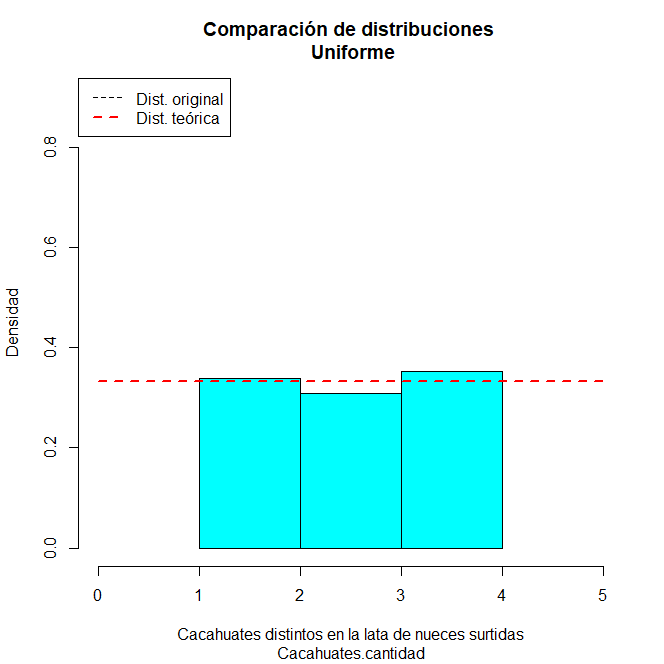
\includegraphics[scale=0.35]{Problema_107.png}
 \end{center}
 el cual incluyen la regi\'on de rechazo $\chi^2 > 9.2103404$,
 donde $\chi^2 = \sum_{i=0}^{k-1} \frac{\left( o_i - e_i \right)^2}{e_i}$,
 que se distribuye como una $\chi^2$ con $v=2$ grados de libertad,
 y el valor calculado del estad\'{\i}stico $\chi^2 = 3.280236$,
 junto con la decisi\'on que es clara, que indica que no hay evidencia
 para rechaza la hip\'otesis nula; adem\'as, el programa brinda m\'as
 informaci\'on como el valor $P$, que es igual a $0.1939572$.
 Por lo tanto, se considera que $X$ se ajusta bien a una distribuci\'on
 uniforme; es decir, con un nivel de significancia de $0.01$, se puede
 concluir que las nueces surtidas de los tres distribuidores
 contienen proporciones iguales de cacahuates.
 que es a lo que se quer\'{\i}a llegar.${}_{\blacksquare}$
\end{solucion}

 \item \begin{enunciado}
 Un grupo de consumidores est\'a interesado en comparar los costos de operaci\'on para dos diferentes tipos de motor para autom\'ovil. El grupo es capaz de encontrar $15$ propietarios cuyos autom\'oviles tienen motor tipo $A$ y $15$ que tienen motor tipo $B$. Los $30$ propietarios compraron sus autom\'oviles en aproximadamente el mismo tiempo y todos llevan buenos registros por cierto periodo de 12 meses. Adem\'as, se encontr\'o que los propietarios recorrieron aproximadamente el mismo n\'umero de millas. Los estad\'{\i}sticos de costo son $\bar{y}_A = \$87.00/1,000$ millas $\bar{y}_B = \$75.00/1,000$ millas, $s_A = \$5.99$, y $s_B = \$4.85$. Calcule un intervalo de confianza de $95\%$ para estimar $\mu_A - \mu_B$, la diferencia en el costo medio de operaci\'on. Suponga normalidad e igual varianza.
\end{enunciado}

\begin{solucion}
 Sean $Y_A$ y $Y_B$ las variables aleatorias de costos de operaci\'on para los tipos de motor para autom\'ovil $A$ y $B$, respectivamente, entonces, del enunciado, se tiene el siguiente resumen de datos:
 \begin{itemize}
  \item $Y_i \sim n\left( \mu_i, \sigma_i \right)$, para cada $i \in \{ A, B \}$.
  \item $\mu_i$ y $\sigma_i$ son desconocidos, para cada $i \in \{ A, B \}$.
  \item $\sigma_A = \sigma_B$.
  \item $n_A = n_B = 15$.
  \item $\bar{y}_A = 87$ d\'olares por cada mil millas y $\bar{y}_B = 75$ d\'olares por cada mil millas.
  \item $s_A = 5.99$ d\'olares y $s_B = 4.85$ d\'olares.
  \item $\alpha = 0.05$.
 \end{itemize}
 Como se desea encontrar un intervalo de confianza bilateral para $\mu_A - \mu_B$, usando como estimador $\bar{y}_A - \bar{y}_B$, desconociendo las varianzas poblacionales aunque suponi\'endolas iguales, con muestras peque\~nas de poblaciones que se distribuyen aproximadamente normal, entonces se requeri\'a del valor $t_{\alpha/2, n_A + n_B - 2} = t_{0.025,28}$. De la Tabla A.4, se tiene que $t_{0.025,28} = 2.048$, mientras que, usando R, se obtiene el valor con los siguientes comandos:
 \begin{verbatim}
> options(digits=22)
> qt(0.025,28,lower.tail=F)
[1] 2.048407141795244967852
 \end{verbatim}
 \vspace{-0.5cm}
 por lo que tambi\'en se puede considerar como $2.04840714$.
 \par Ya que se busca un intervalo de confianza para la diferencia de las medias poblacionales usando como estimador la diferencia de las medias muestrales en muestras peque\~nas, en donde se desconoce las desviaciones est\'andar poblacionales pero suponiendo que son iguales y donde se suponen que las poblaciones se distribuyen aproximadamentenormal, entonces se usar\'a la siguiente formulaci\'on:
 \begin{equation*}
  \left( \bar{y}_A - \bar{y}_B \right) - t_{\alpha/2,n_A+n_B-2}s_p\sqrt{\frac{1}{n_A} + \frac{1}{n_B}} < \mu_A - \mu_B < \left( \bar{y}_A - \bar{y}_B \right) + t_{\alpha/2,n_A+n_B-2}s_p\sqrt{\frac{1}{n_A} + \frac{1}{n_B}}
 \end{equation*}
 en donde
 \begin{equation*}
  s_p = \sqrt{\frac{\left( n_A - 1 \right)s_A^2 + \left( n_B - 1 \right)s_B^2}{n_A + n_B - 2}}
 \end{equation*}
 Por lo tanto, usando los datos obtenidos, considerando el valor $t_{\alpha/2,n_A+n_B - 2}$ del libro, se tienen los c\'alculos de los l\'{\i}mites de confianza como siguen:
 \begin{eqnarray*}
  s_p & = & \sqrt{\frac{\left( n_A - 1 \right)s_A^2 + \left( n_B - 1 \right)s_B^2}{n_A + n_B - 2}} = \sqrt{\frac{(15-1)5.99^2 + (15-1)4.85^2}{15 + 15 - 2}} \\
  & = & \sqrt{\frac{14( 35.8801 + 23.5225)}{28}} = \sqrt{\frac{59.4026}{2}} = \sqrt{\frac{594\,026}{20\,000}} = \sqrt{\frac{297\,013}{10\,000}} \\ 
  & = & \frac{\sqrt{297\,013}}{100}
 \end{eqnarray*}
 y
 \begin{eqnarray*}
  \left( \bar{y}_A - \bar{y}_B \right) \pm t_{\alpha/2,n_A+n_B-2}s_p\sqrt{\frac{1}{n_A} + \frac{1}{n_B}} & = & (87 - 75) \pm 2.048\left( \frac{\sqrt{297\,013}}{100} \right) \left( \sqrt{\frac{1}{15} + \frac{1}{15}}\right) \\
  & = & 12 \pm  \frac{\cancelto{64}{256}}{125} \, \left( \frac{\sqrt{297\,013}\sqrt{2}}{\cancelto{25}{100}\,\sqrt{15}} \right) = 12 \pm \frac{64\sqrt{594\,026}\sqrt{15}}{3\,125(15)} \\
  & = & 12 \pm \frac{64\sqrt{8\,910\,390}}{46\,875} = 12 \pm 0.001365\overline{3}\sqrt{8\,910\,390} \\
  & \approx & 12 \pm 4.075557735
 \end{eqnarray*}
 Por lo tanto, el intervalo de confianza de $95\%$ de la diferencia en el costo medio de operaci\'on para los tipos de motor para autom\'ovil $A$ menos el costo medio de operaci\'on para los tipos de motor para autom\'ovil $B$ es aproximadamente:
 \begin{equation*}
  7.92444226483 < \mu_A - \mu_B < 16.0755577351
 \end{equation*}
 Finalmente, usando R, se puede calcular el intervalo de confianza usando el script en el archivo anexo \texttt{P14\_Intervalo\_de\_confianza\_05.r}, cambiando las siguientes l\'{\i}neas de c\'odigo:
 \begin{verbatim}
> n1<-15
> n2<-15
> m1<-87
> m2<-75
> desv.tipica1<-5.99
> desv.tipica2<-4.85
> alfa<-0.05
> val<-FALSE
> varia<-TRUE
> inter<-'D'
 \end{verbatim}
 \vspace{-0.5cm}
 con lo que se obtiene el siguiente resultado:
 \begin{verbatim}
  n1 n2 media1 media2   LimInf diferencia   LimSup
1 15 15     87     75 7.923632         12 16.07637
 \end{verbatim}
 \vspace{-0.5cm}
 Por lo tanto, al redondear al decimal en que coinciden los resultados anteriores, se tiene que el intervalo de confianza del $95\%$ es $7.924 < \mu_A - \mu_B < 16.076$, que es a lo que se quer\'{\i}a llegar.${}_{\blacksquare}$
\end{solucion}

 \item \begin{enunciado}
 Se realiza un estudio para determinar si hay una diferencia
 entre las proporciones de padres en los estados
 de Maryland (MD), Virginia (VA), Georgia (GA) y Alabama (AL)
 que est\'an a favor de colocar Biblias en las escuelas primarias.
 En la siguiente tabla se registran las respuestas de $100$ padres
 seleccionados al azar en cada uno de esos estados:
 \begin{center}
  \begin{tabular}{lcccc}
   & \multicolumn{4}{c}{\textbf{Estado}} \\
   \cline{2-5}
   \textbf{Preferencia} & \textbf{MD} & \textbf{VA} & \textbf{GA} &
   \textbf{AL} \\
   \hline 
   S\'{\i} & $65$ & $71$ & $78$ & $82$ \\
   No & $35$ & $29$ & $22$ & $18$
  \end{tabular}
 \end{center}
 ¿Podemos concluir que las proporciones de padres que est\'an a favor
 de colocar Biblias en las escuelas son las mismas
 para estos cuatro estados?
 Utilice un nivel de significancia de $0.01$.
\end{enunciado}

\begin{solucion}
 El problema corresponde a una prueba de varias proporciones,
 el cual se resuelve usando una prueba $\chi^2$ como se hace con la prueba
 de homogeneidad, con $(r-1)\times(c-1) = (2-1)\times (4-1) = 3$ grados
 de libertad. As\'{\i} que, nombrando $p_1$, $p_2$, $p_3$ y $p_4$
 a las proporciones de padres que est\'an a favor de colocar Biblias
 en las escuelas primarias en los estados de Maryland, Virginia, Georgia
 y Alabama, respectivamente, la prueba se escribe como sigue:
 \begin{eqnarray*}
  H_0: & & p_1 = p_2 = p_3 = p_4 \\
  H_1: & & \text{no todos las proporciones } p_1, p_2, p_3 \text{ y } p_4
  \text{ son iguales.}
 \end{eqnarray*}
 con un nivel de significancia $\alpha = 0.01$.
 Esto genera la regi\'on de rechazo $\chi^2 > 11.345$, 
 que corresponde al valor cr\'{\i}tico de la distribuci\'on $\chi^2$
 con $3$ grados de libertad.
 \par 
 El proceso se puede realizar usando el programa de R escrito
 en el archivo adjunto con el nombre
 \texttt{P18\_Prueba\_de\_independencia\_y\_homogeneidad\_01.r},
 que, a su vez, usa la base de datos en el archivo nombrado
 \texttt{DB40\_Problema\_109.csv}, con los siguientes cambios:
 \begin{verbatim}
> datos<-read.csv("DB40_Problema_109.csv",sep=";",encoding="UTF-8")
> varInteres<-c("Preferencia","Estado")
> varFrecuencia<-"Frecuencia"
> pruebas<-c(1)
 \end{verbatim}
 \vspace{-0.5cm}
 el programa de R lanza el siguiente resultado:
 \begin{verbatim}
$tabla
           Estado
Preferencia AL GA MD VA
         No 18 22 35 29
         Sí 82 78 65 71

$listaPruebas
$listaPruebas[[1]]

	Pearson's Chi-squared test

data:  tbl1
X-squared = 8.8358, df = 3, p-value = 0.03156
 \end{verbatim}
 \vspace{-0.5cm}
 Con lo que se obtiene un valor del estad\'{\i}stico $\chi^2 = 8.8358$,
 lo cual lleva a decidir no rechazar $H_0$ y concluir,
 con un nivel de significancia de $0.01$, 
 que la proporci\'on de padres que est\'an a favor de colocar Biblias
 en las escuelas no son significantivamente diferentes.
 Sin embargo, n\'otese que el valor $P$ para el valor del estad\'{\i}stico
 obtenido corresponde a una probabilidad de $0.03156$,
 que es bastante bajo.
 Esto indica que existe un riesgo que hay que asumir
 ante la decisi\'on de no rechazar la hip\'otesis nula,
 que es a lo que se quer\'{\i}a llegar.${}_{\blacksquare}$
\end{solucion}

 \item \begin{enunciado}
 Se lleva a cabo un estudio en el Centro de Medicina Veterinaria Equina
 de la Universidad Regional de Virgini-Maryland, para determinar
 si la realizaci\'on de cierto tipo de cirug\'{\i}a en caballos j\'ovenes
 tiene alg\'un efecto en ciertas clases de c\'elulas sangu\'{\i}neas
 en el animal.
 Se toman muestras del fluido de cada uno de seis potros antes y despu\'es
 de la cirug\'{\i}a.
 Se analizan las muestras para el n\'umero de leucogramos
 de gl\'obulos blancos (\texttt{WBC}) posoperatorios.
 Tambi\'en se realiza una medici\'on de leucogramos \texttt{WBC}
 preoperatorios.
 Utilice una prueba $t$ de una muestra pareada
 para determinar si hay un cambio significativo en los leucogramos
 \texttt{WBC} con la cirug\'{\i}a.
 \begin{center}
  \begin{tabular}{ccc}
   \textbf{Potro} & \textbf{Precirug\'{\i}a*} & \textbf{Postcirug\'{\i}a*}
   \\
   \hline 
   1 & $10.80$ & $10.60$ \\
   2 & $12.90$ & $16.60$ \\
   3 & $ 9.59$ & $17.20$ \\
   4 & $ 8.81$ & $14.00$ \\
   5 & $12.00$ & $10.60$ \\
   6 & $ 6.07$ & $ 8.60$ \\
   \hline
   \multicolumn{3}{l}{*Todos los valores $\times 10^{-3}$.}
  \end{tabular}
 \end{center}
\end{enunciado}

\begin{solucion}
 Como se menciona en el ejercicio, el procedimiento corresponde
 a una prueba de muestras pareada.
 Para ello, primero habr\'a que verificar que las muestras provienen
 de poblaciones normales.
 Esto es, antes que todo, probar la hip\'otesis nula que se enuncia como: $X_1$ y $X_2$, las variables aleatorias correspondientes
 a las mediciones de WBC preoperatorios y posoperatorios,
 tienen distribuciones normales, contra la hip\'otesis alternativa,
 de que no es as\'{\i}.
 \par 
 El proceso que generalmente se usa para probar la normalidad 
 se encuentra registrado en el archivo anexo
 \texttt{P17\_Prueba\_de\_normalidad\_01.r}
 que, en este caso, usar\'{\i}a el archivo 
 \texttt{DB41\_Problema\_110.csv} que contiene la base de datos
 escritos en la tabla;
 sin embargo, se trata de muy pocos datos
 y el programa causa un error debido que,
 al colapsar las frecuencias para tener al menos una frecuencia esperada
 de 5 unidades por clase, se obtiene una \'unica clase,
 lo cual no permite realizar la prueba $\chi^2$
 por no tener una valor positivo de grados de libertad.
 Por lo tanto, se proceder\'a a hacer la prueba de Geary
 con las siguientes l\'{\i}neas de c\'odigo junto con sus resultados:
 \begin{verbatim}
> datos<-read.csv("DB41_Problema_110.csv",sep=";",encoding="UTF-8")
> varInteres<-"WBC.cantidad"; distincion<-"Muestra"
> lista<-split(datos[,varInteres],datos[,distincion])
> x<-lista$Precirugía
> y<-lista$Postcirugía
> n1<-length(x); n2<-length(y)
> U1<-sqrt(pi/2)*mean(abs(x-mean(x)))/sqrt(var(x)*(n1-1)/n1)
> U2<-sqrt(pi/2)*mean(abs(y-mean(y)))/sqrt(var(y)*(n2-1)/n2)
> x.Geary.statistic<-(U1-1)/(0.2661/sqrt(n1))
> y.Geary.statistic<-(U2-1)/(0.2661/sqrt(n2))
> x.Geary.p.value<-2*pnorm(abs(x.Geary.statistic),lower.tail=FALSE)
> y.Geary.p.value<-2*pnorm(abs(y.Geary.statistic),lower.tail=FALSE)
> print("P-valor de datos precirugía usando la prueba de Geary"); x.Geary.p.value
[1] "P-valor de datos precirugía usando la prueba de Geary"
[1] 0.6601252
> print("P-valor de datos precirugía usando la prueba de Geary"); y.Geary.p.value
[1] "P-valor de datos precirugía usando la prueba de Geary"
[1] 0.1278513
 \end{verbatim}
 \vspace{-0.5cm}
 Lo cual indica un buen ajuste a una normal de los datos precirug\'{\i}a
 y postcirug\'{\i}a, al tener, en ambos casos, valores $P$ mayores a 0.1.
 \par 
 Ahora que se tienen las condiciones iniciales, la prueba con muestras
 pareadas se puede realizar definiendo primero la hip\'otesis de prueba:
 \begin{eqnarray*}
  H_0: & & \mu_D = \mu_1 - \mu_2  =   0 \\
  H_1: & & \mu_D = \mu_1 - \mu_2 \neq 0
 \end{eqnarray*}
 usando el estad\'{\i}stico $t$ con $n_1 + n_2 - 2 = 10$ grados
 de libertad.
 Entonces, los valores de los c\'alculos se pueden obtener
 usando el archivo anexo
 \texttt{P06\_Prueba\_de\_dos\_medias\_02.r},
 que a su vez usa la base de datos en el archivo ya mencionado
 \texttt{DB41\_Problema\_110.csv}, con los siguientes cambios:
 \begin{verbatim}
> datos<-read.csv("DB41_Problema_110.csv",sep=";",encoding="UTF-8")
> varInteres<-c("WBC.cantidad")
> varSel<-c("Muestra")
> mu<-0
> desv.iguales<-NULL
> alfa<-NULL
> cola<-'D'
> par<-TRUE
 \end{verbatim}
 \vspace{-0.5cm}
 con lo que se obtiene el siguiente resultado:
 \begin{verbatim}
          Var1 Freq Poblaciones H0 n diferencia desv.par error.est grados alpha
1 WBC.cantidad    6    Pareadas  0 6     -2.905  3.35574  1.369975      5  0.05
      PValor Estadistico RegionRechazoInfT RegionRechazoSupT RegionRechazoInfX
1 0.08745276   -2.120477         -2.570582          2.570582         -3.521633
  RegionRechazoSupX
1          3.521633
 \end{verbatim}
 \vspace{-0.5cm}
 Lo cual muestra el valor del estad\'{\i}stico $t = -2.120477$,
 cuyo valor $P$ es $0.08745276$, el cual rechazar\'{\i}a la hip\'otesis
 nula si se considerara una significancia menor $0.0874528$.
 En este caso, como la prueba es de dos colas, el cual se sabe
 no es tan riguroso sobre cu\'ando rechazar una hip\'otesis nula, 
 entonces se considera este valor $P$ lo suficientemente alto
 como para decidir en este caso rechazar la hip\'otesis nula
 y, por lo tanto, concluir que s\'{\i} hay un cambio significativo
 en los leucogramos WBC con la cirug\'{\i}a,
 que es a lo que se quer\'{\i}a llegar.${}_{\blacksquare}$
\end{solucion}

 \item \begin{enunciado}
 Cierto proveedor fabrica un tipo de esfera de goma que vende a las compa\~n\'{\i}as automotrices. En la aplicaci\'on, las piezas del material deben tener ciertas caracter\'{\i}sticas de dureza. Ocasionalmente, se detectan las esferas defectuosas y se rechazan. El proveedor afirma que la proporci\'on de defectuosas es $0.05$. El desaf\'{\i}o lleg\'o de un cliente que compr\'o el producto. De manera que se realiz\'o un experimento donde se probaron $400$ esferas y se encontraron $17$ defectuosas.
 \begin{enumerate}
  \item Calcule un intervalo de confianza bilateral de $95\%$ en la proporci\'on de defectuosos.
  
  \item Calcule un intervalo de confianza unilateral de $95\%$ adecuado en la proporci\'on de defectuosos.
  
  \item Interprete los intervalos de ambos incisos y comente acerca de la afirmaci\'on hecha por el proveedor.
 \end{enumerate}
\end{enunciado}

\begin{solucion}
 Sea $X$ la variable aleatoria de la cantidad de esferas de goma que fabrica el proveedor del enunciado  que salen defectuosas de entre un total de $n$ pelotas fabricadas por este proveedor, entonces $\widehat{P} = X/n$ es un estad\'{\i}stico de proporci\'on del experimento binomial que estima al valor $p$, la proporci\'on real de pelotas de goma defectuosas entre las fabricadas por el proveedor, entonces, del enunciado, se tienen los siguientes datos obtenidos de una muestra:
 \begin{itemize}
  \item $n = 400$.
  \item $x = 17$.
 \end{itemize}
 por lo que $\hat{p}$, la proporci\'on de \'exito en esta muestra, y $\hat{q} = 1 - \hat{p}$ valen:
 \begin{itemize}
  \item $\hat{p} = \frac{17}{400} = 0.0425$; y,
  \item $\hat{q} = 1 - \frac{17}{400} = \frac{383}{400} = 0.9575$.
 \end{itemize}
 Con lo que los incisos se resuleven como sigue.
 \begin{enumerate}
  \item Sea $\alpha$ el nivel de confianza del intervalo de confianza bilateral para $p$, entonces
  \begin{itemize}
   \item $\alpha = 0.05$.
  \end{itemize}
  Adem\'as, como se buscar\'a un intervalo de confianza para estimar $p$, entonces se requiere del valor $z_{\alpha/2} = z_{0.025}$, el cual se calcul\'o en el ejercicio 9.5 y su aproximaci\'on es de $1.96$, aunque, en R, se puede considerar con mayor precisi\'on como $1.95996398454$.
  \par 
  Ya que se busca un intervalo bilateral para la proporci\'on $p$, en donde el tama\~no de las muestras es grande y se tiene que $n\hat{p}$ y $n\hat{q}$ son ambos mayores a $5$, entonces se usar\'a la f\'ormula de intervalo siguiente:
  \begin{equation*}
   \hat{p} - z_{\alpha/2}\sqrt{\frac{\hat{p}\hat{q}}{n}} < p < \hat{p} + z_{\alpha/2}\sqrt{\frac{\hat{p}\hat{q}}{n}}
  \end{equation*}
  Por lo tanto, usando los datos obtenidos y con la primera aproximaci\'on de $z_{\alpha/2}$, se tiene los siguientes c\'alculos de los l\'{\i}mites del intervalo de confianza como sigue:
  \begin{eqnarray*}
   \hat{p} \pm z_{\alpha/2}\sqrt{\frac{\hat{p}\hat{q}}{n}} & = & \frac{17}{400} \pm 1.96\sqrt{\frac{(17/400)(383/400)}{400}} = \frac{17}{400} \pm \frac{49}{25} \sqrt{\frac{6\,511}{400^3}} = \frac{17}{400} \pm \frac{49\sqrt{6\,511}}{25(8\,000)} \\
   & = & \frac{17}{400} \pm \frac{49\sqrt{6\,511}}{200\,000} = 0.0425 \pm 0.000245\sqrt{6\,511} \approx 0.0425 \pm 0.0197692
  \end{eqnarray*}
  Por lo tanto, el intervalo de confianza bilateral de $95\%$ de la proporci\'on de pelotas de goma defectuosas entre las fabricadas por el proveedor es aproximadamente:
  \begin{equation*}
   0.02273076 < p < 0.0622692
  \end{equation*}
  Por otro lado, usando R, se puede calcular el intervalo de confianza usando el script en el archivo anexo \texttt{P17\_Intervalo\_de\_confianza\_08.r} cambiando las siguientes l\'{\i}neas de c\'odigo:
  \begin{verbatim}
> n<-400
> x<-17
> p<-NULL
> alfa<-0.05
> inter<-'D'
  \end{verbatim}
  \vspace{-0.5cm}
  con lo que se obtiene el siguiente resultado:
  \begin{verbatim}
     LimInf Proporción    LimSup
1 0.0227311     0.0425 0.0622689
  \end{verbatim}
  \vspace{-0.5cm}
  Por lo que, al redondear al decimal en que coinciden los resultados anteriores, se tiene que el intervalo de confianza del $95\%$ es $0.02273 < p < 0.06227$.${}_{\square}$
  
  \item Sea ahora $\alpha$ el nivel de confianza del intervalo de confianza unilateral para $p$, entonces
  \begin{itemize}
   \item $\alpha = 0.05$.
  \end{itemize}
  Como se buscar\'a un intervalo de confianza unilateral para estimar $p$, entonces se requiere del valor $z_{\alpha} = z_{0.05}$, el cual se calcul\'o en el ejericio 9.30 y su aproximaci\'on es de $1.645$, aunque, en R, se puede considerar con mayor precisi\'on como $1.644853626951$.
  \par Ya que se busca un intervalo unilateral superior para la proporci\'on $p$, en donde el tama\~no de las muestras es grande y se tiene que $n\hat{p}$ y $n\hat{q}$ son ambos mayores a $5$, entonces se usar\'a la f\'ormula de intervalo siguiente:
  \begin{equation*}
   p < \hat{p} + z_{\alpha}\sqrt{\frac{\hat{p}\hat{q}}{n}}
  \end{equation*}
  Por lo tanto, usando los datos obtenidos y con la primera aproximaci\'on de $z_{\alpha}$, se tiene los siguientes c\'alculos del intervalo de confianza unilateral superior como sigue:
  \begin{eqnarray*}
   \hat{p} + z_{\alpha}\sqrt{\frac{\hat{p}\hat{q}}{n}} & = & \frac{17}{400} + 1.645\sqrt{\frac{(17/400)(383/400)}{400}} = \frac{17}{400} + \frac{329\sqrt{6\,511}}{200(8\,000)} \\ 
   & = & \frac{17}{400} + \frac{329\sqrt{6\,511}}{1\,600\,000} = 0.0425 + 0.000205625\sqrt{6\,511} \approx 0.0425 + 0.016592
  \end{eqnarray*}
  Por lo tanto, el intervalo unilateral superior de $95\%$ de la proporci\'on de pelotas de goma defectuosas entre las fabricadas por el proveedor es aproximadamente:
  \begin{equation*}
   p < 0.059092
  \end{equation*}
  Por otro lado, usando R, se puede calcular el intervalo de confianza unilateral superior usando el script en el archivo \texttt{P17\_Intervalo\_de\_confianza\_08.r} cambiando las siguientes l\'{\i}neas de c\'odigo:
  \begin{verbatim}
> n<-400
> x<-17
> p<-NULL
> alfa<-0.05
> inter<-'S'
  \end{verbatim}
  \vspace{-0.5cm}
  con lo que se obtiene el siguiente resultado:
  \begin{verbatim}
     LimInf Proporción    LimSup
1 0.0259094     0.0425 0.0590906
  \end{verbatim}
  \vspace{-0.5cm}
  Por lo que, al redondear al decimal en que coinciden los resultados anteriores, se tiene que el intervalo de confianza unilateral superior del $95\%$ es $ p < 0.05909$.${}_{\square}$
  
  \item Los resultados anteriores, sugieren que el proveedor est\'a dando un resultado cercano a la realidad, con la posibilidad de que se \'este el valor real, ya que la proporci\'on de pelotas defetuosas se encuentra, seg\'un los intervalos calculados, aproximadamente entre el $2\%$ y $6\%$ de las pelotas fabricadas, que es a lo que se quer\'{\i}a llegar.${}_{\blacksquare}$
 \end{enumerate}

\end{solucion}

 \item \begin{enunciado}
 En un estudio que realiza el Departamento de Ingenier\'{\i}a Mec\'anica y que analiza el Centro de Consulta Estad\'{\i}stica del Instituto Polit\'ecnico y Universidad Estata de Virginia, se comparan las varillas de acero que proveen dos compa\~n\'{\i}as diferentes.
 Se fabrican diez resortes de muestra con las varillas proporcionadas por cada compa\~n\'{\i}a y se estudia la ``capacidad de rebote''.
 Los datos son los siguientes:
 \begin{verbatim}
Compañía A
 9.3 8.8 6.8  8.7  8.5 6.7  8.0  6.5  9.2 7.0
Compañía B
11.0 9.8 9.9 10.2 10.1 9.7 11.0 11.1 10.2 9.6
 \end{verbatim}
 \vspace{-0.5cm}
 ¿Puede concluir que casi no hay diferencia entre las varillas de acero proporcionadas por las dos compa\~n\'{\i}as?
 Utilice un valor $P$ para llegar a su conclusi\'on.
 ¿Las varianzas deber\'{\i}an combinarse aqu\'{\i}?
\end{enunciado}

\begin{solucion}
 Para realizar una prueba de diferencia de medias con pocos datos
 (menos de 30), el estad\'{\i}stico usado requiere una condici\'on inicial
 que es la suposici\'on de que las muestras provengan de poblaciones
 con distribuci\'on normal.
 Entonces se realizar\'an dos pruebas de bondad de ajuste
 para verificar que, en efecto, las muestras provienen de poblaciones
 normales. Entonces, la hip\'otesis nula para estas pruebas se pueden
 escribir de la forma
 $X_i$ sigue una distribuci\'on normal, para cada $i \in \{1,2\}$,
 donde $X_1$ y $X_2$ representan las medidas poblacionales de capacidad
 de rebote de los resortes de las compa\~n\'{\i}as A y B,
 respectivamente, contra la hip\'otesis alternativa
 de que $X_i$, para cada $i \in \{1,2\}$ no sigue una distribuci\'on
 normal.
 \par 
 Debido a que la muestra es peque\~na y no se consideran par\'ametros
 en la suposici\'on de las normalidades,
 la prueba con $\chi^2$ crea insuficientes clases, en cada muestra,
 que al calcular los grados de libertad junto con los grados que se restan
 por no considerar par\'ametros previos, entonces se obtiene
 un valor negativo, lo cual no puede corresponde a grados de libertad.
 Por lo tanto, se proceder\'a a realizar las pruebas de Geary,
 simult\'aneamente, con las siguientes l\'{\i}neas de c\'odigo
 escritas en R, que usa la base de datos
 \texttt{DB42\_Problema\_111.csv},
 que se presenta a continuaci\'on junto con los resultados:
 \begin{verbatim}
> datos<-read.csv("DB43_Problema_112.csv",sep=";",encoding="UTF-8")
> varInteres<-"Rebote.capacidad"; distincion<-"Compañía"
> lista<-split(datos[,varInteres],datos[,distincion])
> x<-lista$A; y<-lista$B
> n1<-length(x); n2<-length(y)
> U1<-sqrt(pi/2)*mean(abs(x-mean(x)))/sqrt(var(x)*(n1-1)/n1)
> U2<-sqrt(pi/2)*mean(abs(y-mean(y)))/sqrt(var(y)*(n2-1)/n2)
> x.Geary.statistic<-(U1-1)/(0.2661/sqrt(n1))
> y.Geary.statistic<-(U2-1)/(0.2661/sqrt(n2))
> x.Geary.p.value<-2*pnorm(abs(x.Geary.statistic),lower.tail=FALSE)
> y.Geary.p.value<-2*pnorm(abs(y.Geary.statistic),lower.tail=FALSE)
> print("P-valor para los productos de la compañia A usando la prueba de Geary")
[1] "P-valor para los productos de la compañia A usando la prueba de Geary"
> x.Geary.p.value
[1] 0.06671429
> print("P-valor para los productos de la compañia B usando la prueba de Geary")
[1] "P-valor para los productos de la compañia B usando la prueba de Geary"
> y.Geary.p.value
[1] 0.3699307
 \end{verbatim}
 \vspace{-0.5cm}
 Esto indica un buen ajuste a una distribuci\'on normal
 para la poblaci\'on de la capacidad de rebote de los productos
 de la compa\~n\'{\i}a B;
 sin embargo, la poblaci\'on de esta capacidad para los productos
 de la compa\~n\'{\i}a A
 muestran un valor $P$ de $0.06671429$ para el ajuste de bondad.
 Se tomar\'a el riesgo ante la baja probabilidad
 y se tomar\'a la decisi\'on de suponer que ambas muestras vienen
 de poblaciones con distribuciones normales.
 \par
 Para la prueba, se requiere ahora saber si las varianzas poblacionales
 de donde vienen ambas muestras se deben de considerar iguales
 o diferentes. Este implica una prueba de proporci\'on de varianzas,
 cuya hip\'otesis nula se puede enunciar como
 $H_0: \, \frac{\sigma_1}{\sigma_2} = 1$, contra la hip\'otesis
 alternativa $H_1: \, \frac{\sigma_1}{\sigma_2} \neq 1$,
 donde $\sigma_1$ y $\sigma_2$ representan las varianzas poblacionales
 de $X_1$ y $X_2$, respectivamente.
 Para ello se hace una prueba $F$ con ayuda del archivo adjunto
 \texttt{P14\_Prueba\_de\_dos\_varianzas\_02.r},
 que a su vez usa el archivo \texttt{DB43\_Problema\_112.csv},
 con los siguientes cambios:
 \begin{verbatim}
> datos<-read.csv("DB43_Problema_112.csv",sep=";",encoding="UTF-8")
> varInteres<-c("Rebote.capacidad")
> varSel<-c("Compañía")
> alfa<-NULL
> cola<-'D'
 \end{verbatim}
 \vspace{-0.5cm}
 lo cual arroja el siguiente resultado:
 \begin{verbatim}
          variable Freq n1 n2 media1 media2 varianza1 varianza2 v1 v2 alpha
1 Rebote.capacidad   20 10 10   7.95  10.26  1.207222 0.3248889  9  9  0.05
     PValor Estadistico             RegionRechazo
1 0.0637265      3.7158 < 0.2483859 y > 4.0259942
 \end{verbatim}
 \vspace{-0.5cm}
 en donde se observa que el estad\'{\i}stico $F=\frac{\sigma_1}{\sigma_2}$
 toma el valor de $3.7158$ con $v_1 = 9$ y $v_2 = 9$ grados
 de libertad para la distribuci\'on $F$,
 obteniendo as\'{\i} un valor $P$ de $0.0637265$,
 lo cual, aunque no es muy alto, es suficiente para decidir rechazar
 la hip\'otesis nula y, por lo tanto, se puede suponer que las varianzas iguales para la prueba $t$.
 \par 
 Para la prueba se enuncia la hip\'otesis nula como sigue:
 \begin{eqnarray*}
  H_0: & & \mu_1 - \mu_2   =   0 \\
  H_1: & & \mu_1 - \mu_2 \neq  0
 \end{eqnarray*}
 donde $\mu_1$ y $\mu_2$ representan las medias poblacionales
 de $X_1$ y $X_2$, respectivamente.
 El estad\'{\i}stico y el valor $P$ se calculan con ayuda
 del archivo adjunto \texttt{P06\_Prueba\_de\_dos\_medias\_02.r},
 que nuevamente usan la base de datos almacenado en el archivo adjunto
 \texttt{DB43\_Problema\_112.csv}, con los siguientes cambios:
 \begin{verbatim}
> datos<-read.csv("DB43_Problema_112.csv",sep=";",encoding="UTF-8")
> varInteres<-c("Rebote.capacidad")
> varSel<-c("Compañía")
 mu<-0
> desv.iguales<-TRUE
> alfa<-NULL
> cola<-'D'
> par<-FALSE
 \end{verbatim}
 \vspace{-0.5cm}
 lo cual arroja el siguiente resultado:
 \begin{verbatim}
              Var1 Freq    Poblaciones H0  valorPVar     suposicionVar n1 n2
1 Rebote.capacidad   20 Independientes  0 0.06372648 Var no diferentes 10 10
  media1 media2 diferencia desv.est1 desv.est2   est.sp error.est grados alpha
1   7.95  10.26      -2.31  1.098737 0.5699903 0.875246 0.3914219     18  0.05
        PValor Estadistico RegionRechazoInfT RegionRechazoSupT RegionRechazoInfX
1 1.379592e-05    -5.90156         -2.100922          2.100922        -0.8223469
  RegionRechazoSupX
1         0.8223469
 \end{verbatim}
 \vspace{-0.5cm}
 de donde se observa que el valor del estad\'{\i}stico
 es $t = -5.90156$, con un valor $P$ aproximado
 de $1.379592\times 10^{-5}$, 
 lo cual, al ser tan bajo, y teniendo en cuenta que $\bar{x}_1 = 7.95$
 y $\bar{x}_2 = 10.26$, se concluye que la capacidad de rebote promedio
 de los resortes son diferentes entre ambas compa\~n\'{\i}as,
 siendo que los resortes de la compa\'{\i}a A tiene una capacidad
 de reborte menor que los resortes de la compa\~n\'{\i}a B,
 que es a lo que se quer\'{\i}a llegar.${}_{\blacksquare}$
\end{solucion}

 \item \begin{enunciado}
 En un estudio que conduce el Centro de Recursos Acu\'aticos
 y que analiza el Centro de Consulta Estad\'{\i}stica
 del Instituto Polit\'ecnico y Universidad Estatal de Virginia,
 se comparan dos plantas de tratamiento para aguas residuales.
 La planta \textit{A} se ubica donde el ingreso medio de los hogares
 est\'a por abajo de $\$22,000$ al a\~no,
 y la planta \textit{B} se ubica donde el ingreso medio de los hogres
 est\'a por arriba de $\$60,000$ anuales.
 La cantidad de agua residual que trata cada planta
 (miles de galones/d\'{\i}a) se muestra de forma aleatoria
 durante 10 d\'{\i}as.
 Los datos son los siguientes:
 \begin{verbatim}
Planta A:
21 19 20 23 22 28 32 19 13 18
Planta B:
20 39 24 33 30 28 30 22 33 24
 \end{verbatim}
 \vspace{-0.5cm}
 ¿Con un nivel de significancia de $5\%$ podemos concluir que la cantidad promedio de agua residual tratada en el vecindario de altos ingresos es mayor que la del \'area de bajos ingresos?
\end{enunciado}

\begin{solucion}
 Para realizar una prueba de diferencia de medias con menos de 30 datos,
 se requiere la suposici\'on de que las muestras provengan de poblaciones
 con distribuci\'on normal.
 Para validar el uso de la prueba de dos medias, se realizar\'an pruebas
 de bondad de ajuste que indiquen si las muestras provienen de poblaciones
 normales.
 Entonces, la hip\'otesis nula para estas pruebas se pueden
 escribir de la forma: $X_i$ sigue una distribuci\'on normal,
 para cada $i \in \{1,2\}$,
 donde $X_1$ y $X_2$ representan los cantidades de agua residual,
 en miles de galones por d\'{\i}a, de las plantas A y B, respectivamente,
 contra la hip\'otesis alternativa de que $X_i$,
 para cada $i \in \{1,2\}$, no sigue una distribuci\'on normal.
 \par 
 Debido a que la muestra es peque\~na y no se consideran par\'ametros
 en la suposici\'on de las normalidades,
 la prueba con $\chi^2$ crea insuficientes clases, en cada muestra,
 que al calcular los grados de libertad junto con los grados que se restan
 por no considerar par\'ametros previos, entonces se obtiene
 un valor negativo, lo cual no puede corresponder a grados de libertad.
 Por lo tanto, se proceder\'a a realizar las pruebas de Geary,
 simult\'aneamente, con las siguientes l\'{\i}neas de c\'odigo
 escritas en R, que usa la base de datos
 \texttt{DB44\_Problema\_113.csv},
 que se presenta a continuaci\'on junto con los resultados:
 \begin{verbatim}
> datos<-read.csv("DB44_Problema_113.csv",sep=";",encoding="UTF-8")
> varInteres<-"AguaResidual.KGalPDia"; distincion<-"Planta"
> lista<-split(datos[,varInteres],datos[,distincion])
> x<-lista$A; y<-lista$B
> n1<-length(x); n2<-length(y)
> U1<-sqrt(pi/2)*mean(abs(x-mean(x)))/sqrt(var(x)*(n1-1)/n1)
> U2<-sqrt(pi/2)*mean(abs(y-mean(y)))/sqrt(var(y)*(n2-1)/n2)
> x.Geary.statistic<-(U1-1)/(0.2661/sqrt(n1))
> y.Geary.statistic<-(U2-1)/(0.2661/sqrt(n2))
> x.Geary.p.value<-2*pnorm(abs(x.Geary.statistic),lower.tail=FALSE)
> y.Geary.p.value<-2*pnorm(abs(y.Geary.statistic),lower.tail=FALSE)
> print("P-valor para la planta A usando la prueba de Geary");x.Geary.p.value
[1] "P-valor para la planta A usando la prueba de Geary"
[1] 0.5061923
> print("P-valor para la planta B usando la prueba de Geary");y.Geary.p.value
[1] "P-valor para la planta B usando la prueba de Geary"
[1] 0.4920951
 \end{verbatim}
 \vspace{-0.5cm}
 Esto indica un buen ajuste a una distribuci\'on normal
 para ambas variables aleatorias;
 Por lo tanto, es v\'alido suponer que ambas muestras vienen
 de poblaciones con distribuciones normales.
 \par
 Para la prueba, se requiere ahora saber si las varianzas poblacionales
 de donde vienen ambas muestras se deben de considerar iguales
 o diferentes. Este implica una prueba de proporci\'on de varianzas,
 cuya hip\'otesis nula se puede enunciar como
 $H_0: \, \frac{\sigma_1}{\sigma_2} = 1$, contra la hip\'otesis
 alternativa $H_1: \, \frac{\sigma_1}{\sigma_2} \neq 1$,
 donde $\sigma_1$ y $\sigma_2$ representan las varianzas poblacionales
 de $X_1$ y $X_2$, respectivamente.
 Para ello se hace una prueba $F$ con ayuda del archivo adjunto
 \texttt{P14\_Prueba\_de\_dos\_varianzas\_02.r},
 que a su vez usa el archivo \texttt{DB44\_Problema\_113.csv},
 con los siguientes cambios:
 \begin{verbatim}
> datos<-read.csv("DB44_Problema_113.csv",sep=";",encoding="UTF-8")
> varInteres<-c("AguaResidual.KGalPDia")
> varSel<-c("Planta")
> alfa<-NULL
> cola<-'D'
 \end{verbatim}
 \vspace{-0.5cm}
 lo cual arroja el siguiente resultado:
 \begin{verbatim}
               variable Freq n1 n2 media1 media2 varianza1 varianza2 v1 v2 alpha
1 AguaResidual.KGalPDia   20 10 10   21.5   28.3  28.27778  34.45556  9  9  0.05
     PValor Estadistico             RegionRechazo
1 0.7733006    0.820703 < 0.2483859 y > 4.0259942
 \end{verbatim}
 \vspace{-0.5cm}
 en donde se observa que el estad\'{\i}stico $F=\frac{\sigma_1}{\sigma_2}$
 toma el valor de $0.820703$ con $v_1 = v_2 = 9$ grados
 de libertad para la distribuci\'on $F$,
 obteniendo as\'{\i} un valor $P$ de $0.7733006$,
 lo cual, al ser muy alto, no se rechaza la hip\'otesis nula y,
 por lo tanto, se puede suponer las varianzas iguales para la prueba $t$.
 \par 
 Para la prueba se enuncia la hip\'otesis nula como sigue:
 \begin{eqnarray*}
  H_0: & & \mu_1 - \mu_2 \geq 0 \\
  H_1: & & \mu_1 - \mu_2   <  0
 \end{eqnarray*}
 donde $\mu_1$ y $\mu_2$ representan las medias poblacionales
 de $X_1$ y $X_2$, respectivamente,
 con un nivel de significancia de $\alpha = 0.05$.
 La regi\'on de rechazo, el estad\'{\i}stico y la decisi\'on
 se calculan con ayuda del archivo adjunto
 \texttt{P06\_Prueba\_de\_dos\_medias\_02.r},
 que nuevamente usa la base de datos almacenado en el archivo adjunto
 \texttt{DB44\_Problema\_113.csv}, con los siguientes cambios:
 \begin{verbatim}
> datos<-read.csv("DB44_Problema_113.csv",sep=";",encoding="UTF-8")
> varInteres<-c("AguaResidual.KGalPDia")
> varSel<-c("Planta")
> mu<-0
> desv.iguales<-TRUE
> alfa<-0.05
> cola<-'I'
> par<-FALSE
 \end{verbatim}
 \vspace{-0.5cm}
 lo cual arroja el siguiente resultado:
 \begin{verbatim}
                   Var1 Freq    Poblaciones H0 valorPVar     suposicionVar n1 n2
1 AguaResidual.KGalPDia   20 Independientes  0 0.7733006 Var no diferentes 10 10
  media1 media2 diferencia desv.est1 desv.est2   est.sp error.est grados alpha
1   21.5   28.3       -6.8  5.317685  5.869885 5.600595  2.504662     18  0.05
       PValor Estadistico RegionRechazoInfT RegionRechazoInfX     Resultado
1 0.007096931   -2.714937         -1.734064         -4.343244 Se rechaza H0
 \end{verbatim}
 \vspace{-0.5cm}
 de donde se observa que la regi\'on de rechazo est\'a dado
 para $T < -1.734064$,
 el estad\'{\i}stico obtenido es $t = -2.714937$ y la decisi\'on tomada,
 ya en este punto evidente pero que tambi\'en se muestra en el programa,
 es la de rechazar $H_0$ a favor de $H_1$ y, por lo tanto, concluir
 que, en efecto, la cantidad promedio de agua residual tratada
 en el vecindario de altos ingresos es mayor que la del \'area
 de bajos ingresos, que es a lo que se quer\'{\i}a llegar.${}_{\blacksquare}$
\end{solucion}

 \item \begin{enunciado}
 Los siguientes datos muestran el n\'umero de defectos en 100,000 l\'{\i}neas de c\'odigo en un tipo particular de software hecho en Estados Unidos y Jap\'on.
 ¿Hay suficiente evidencia para afirmar que existe una diferencia significativa entre los programas de los dos pa\'{\i}ses?
 Pruebe las medias.
 ¿Deber\'{\i}an combinarse las varianzas?
 \begin{verbatim}
E.U.    48 39 42 52 40 48 52 52
        54 48 52 55 43 46 48 52
Japón   50 48 42 40 43 48 50 46
        38 38 36 40 40 48 48 45
 \end{verbatim}
 \vspace{-0.5cm}
\end{enunciado}

\begin{solucion}
 Para realizar una prueba de diferencia de medias con menos de 30 datos,
 se requiere la suposici\'on de que las muestras provengan de poblaciones
 con distribuci\'on normal.
 Para validar el uso de la prueba de dos medias, se realizar\'an pruebas
 de bondad de ajuste que indiquen si las muestras provienen de poblaciones
 normales.
 Entonces, la hip\'otesis nula para estas pruebas se pueden
 escribir de la forma: $X_i$ sigue una distribuci\'on normal,
 para cada $i \in \{1,2\}$, contra la hip\'otesis alternativa
 de que $X_i$, para cada $i \in \{1,2\}$, no sigue una distribuci\'on
 normal, donde $X_1$ y $X_2$ representan el n\'umero de defectos
 en $100,000$ l\'{\i}neas de c\'odigo en el software hecho en Estados
 Unidos y en Jap\'on, respectivamente.
 \par 
 Debido a que la muestra es peque\~na y no se consideran par\'ametros
 en la suposici\'on de las normalidades,
 la prueba con $\chi^2$ crea insuficientes clases, en cada muestra,
 que al calcular los grados de libertad junto con los grados que se restan
 por no considerar par\'ametros previos, entonces se obtiene
 un valor negativo, lo cual no puede corresponder a grados de libertad.
 Por lo tanto, se proceder\'a a realizar las pruebas de Geary,
 simult\'aneamente, con las siguientes l\'{\i}neas de c\'odigo
 escritas en R, que usa la base de datos
 \texttt{DB45\_Problema\_114.csv},
 que se presenta a continuaci\'on junto con los resultados:
 \begin{verbatim}
> datos<-read.csv("DB45_Problema_114.csv",sep=";",encoding="UTF-8")
> varInteres<-"Errores.PKLineas"; distincion<-"País"
> lista<-split(datos[,varInteres],datos[,distincion])
> x<-lista$EE.UU.; y<-lista$Japón
> n1<-length(x); n2<-length(y)
> U1<-sqrt(pi/2)*mean(abs(x-mean(x)))/sqrt(var(x)*(n1-1)/n1)
> U2<-sqrt(pi/2)*mean(abs(y-mean(y)))/sqrt(var(y)*(n2-1)/n2)
> x.Geary.statistic<-(U1-1)/(0.2661/sqrt(n1))
> y.Geary.statistic<-(U2-1)/(0.2661/sqrt(n2))
> x.Geary.p.value<-2*pnorm(abs(x.Geary.statistic),lower.tail=FALSE)
> y.Geary.p.value<-2*pnorm(abs(y.Geary.statistic),lower.tail=FALSE)
> print("P-valor para los errores en EE.UU. usando la prueba de Geary")
[1] "P-valor para los errores en EE.UU. usando la prueba de Geary"
> x.Geary.p.value
[1] 0.6938
> print("P-valor para los errores en Japón usando la prueba de Geary")
[1] "P-valor para los errores en Japón usando la prueba de Geary"
> y.Geary.p.value
[1] 0.03519627
 \end{verbatim}
 \vspace{-0.5cm}
 Esto indica un buen ajuste a una distribuci\'on normal
 para los datos correspondientes a EE.UU.;
 sin embargo, la poblaci\'on para los datos correspondientes a Jap\'on
 muestran un valor $P$ de $0.03519627$ para el ajuste de bondad.
 Se asumir\'a el riesgo ante la baja probabilidad
 y se tomar\'a la decisi\'on de suponer que ambas muestras vienen
 de poblaciones con distribuciones normales.
 Esto debido a que la prueba $t$ es relativamente robusta
 para la normalidad.
 Por otro lado, aunque la prueba de varianzas que se ver\'a
 a continuaci\'on no es robusta para la normalidad,
 se adelanta que se obtendr\'a un valor $P$ tan alto para dicha prueba
 que se podr\'a suponer sin mucho riesgo que las varianzas poblacionales
 son iguales.
 \par
 Para la prueba $t$, se requiere decidir tambi\'en si se va a suponer
 que las varianzas poblacionales de donde vienen ambas muestras
 son iguales o diferentes.
 Este lleva al an\'alisis a una prueba de proporci\'on de varianzas,
 cuya hip\'otesis nula se puede enunciar como
 $H_0: \, \sigma_1 = \sigma_2$, contra la hip\'otesis alternativa
 $H_1: \, \sigma_1 \neq \sigma_2$, donde $\sigma_1$ y $\sigma_2$
 representan las varianzas poblacionales de $X_1$ y $X_2$,
 respectivamente.
 Para ello se hace una prueba $F$ con ayuda del archivo adjunto
 \texttt{P14\_Prueba\_de\_dos\_varianzas\_02.r},
 que a su vez usa el archivo \texttt{DB45\_Problema\_114.csv},
 con los siguientes cambios:
 \begin{verbatim}
> datos<-read.csv("DB45_Problema_114.csv",sep=";",encoding="UTF-8")
> varInteres<-c("Errores.PKLineas")
> varSel<-c("País")
> alfa<-NULL
> cola<-'D'
 \end{verbatim}
 \vspace{-0.5cm}
 lo cual arroja el siguiente resultado:
 \begin{verbatim}
          variable Freq n1 n2  media1 media2 varianza1 varianza2 v1 v2 alpha
1 Errores.PKLineas   32 16 16 48.1875  43.75   24.9625  21.93333 15 15  0.05
     PValor Estadistico             RegionRechazo
1 0.8054528    1.138108 < 0.3493947 y > 2.8620925
 \end{verbatim}
 \vspace{-0.5cm}
 en donde se observa que el estad\'{\i}stico $F=\frac{\sigma_1}{\sigma_2}$
 toma el valor de $1.138108$ con $v_1 = v_2 = 15$ grados
 de libertad para la distribuci\'on $F$,
 obteniendo as\'{\i} un valor $P$ de $0.8054528$,
 lo cual, al ser muy alto, no se rechaza la hip\'otesis nula y,
 por lo tanto, se puede suponer las varianzas iguales para la prueba $t$.
 \par 
 Para la prueba que concierne a la pregunta planteada en el problema,
 se enuncia la hip\'otesis nula como sigue:
 \begin{eqnarray*}
  H_0: & & \mu_1 - \mu_2   =  0 \\
  H_1: & & \mu_1 - \mu_2 \neq 0
 \end{eqnarray*}
 donde $\mu_1$ y $\mu_2$ representan las medias poblacionales
 de $X_1$ y $X_2$, respectivamente.
 El estad\'{\i}stico y el valor $P$ se calculan con ayuda
 del archivo adjunto \texttt{P06\_Prueba\_de\_dos\_medias\_02.r},
 que nuevamente usa la base de datos almacenado en el archivo adjunto
 \texttt{DB45\_Problema\_114.csv}, con los siguientes cambios:
 \begin{verbatim}
> datos<-read.csv("DB45_Problema_114.csv",sep=";",encoding="UTF-8")
> varInteres<-c("Errores.PKLineas")
> varSel<-c("País")
> mu<-0
> desv.iguales<-TRUE
> alfa<-NULL
> cola<-'D'
> par<-FALSE
 \end{verbatim}
 \vspace{-0.5cm}
 lo cual arroja el siguiente resultado:
 \begin{verbatim}
              Var1 Freq    Poblaciones H0 valorPVar     suposicionVar n1 n2
1 Errores.PKLineas   32 Independientes  0 0.8054528 Var no diferentes 16 16
   media1 media2 diferencia desv.est1 desv.est2   est.sp error.est grados alpha
1 48.1875  43.75     4.4375  4.996249  4.683304 4.842305  1.712013     30  0.05
      PValor Estadistico RegionRechazoInfT RegionRechazoSupT RegionRechazoInfX
1 0.01460178    2.591978         -2.042273          2.042273         -3.496398
  RegionRechazoSupX
1          3.496398
 \end{verbatim}
 \vspace{-0.5cm}
 de donde se observa que el estad\'{\i}stico obtenido es $t = 2.591978$,
 con $v = n_1 + n_2 - 2 = 30$ grados de libertad para la distribuci\'on
 $t$, lo que corresponde a un valor $P$ de $0.01460178$,
 que corresponde a un valor $P$ muy bajo.
 Considerando adem\'as que la prueba es de 2 colas
 y que $\bar{x}_1 = 48.1875$ y $\bar{x}_2 = 43.75$,
 donde las pruebas de dos colas no se consideran tan estrictas,
 por lo que el valor $P$ habr\'{\i}a sido menor para una prueba
 de cola superior, la decisi\'on tomada es rechazara $H_0$
 a favor de $H_1$ y, por lo tanto, concluir que hay evidencia suficiente
 para afirmar que hay una diferencia significativa entre los programas
 de ambos pa\'{\i}ses, siendo el programa de Jap\'on
 el que presenta menos errores por cada mil l\'{\i}neas de c\'odigo,
 que es a lo que se quer\'{\i}a llegar.${}_{\blacksquare}$
\end{solucion}

 \item \begin{enunciado}
 Estudios indican que la concentraci\'on de \texttt{PCB} es mucho
 m\'as alta en tejido maligno de pecho que en tejido normal de pecho.
 Si un estudio de $50$ mujeres con c\'ancer de seno revela
 una concentraci\'on promedio de \texttt{PCB} de $22.8 \times 10^{-4}$
 gramos, con una desviaci\'on est\'andar de $4.8 \times 10^{-4}$ gramos,
 ¿la concentraci\'on media de \texttt{PCB} es menor
 que $24 \times 10^{-4}$ gramos?
\end{enunciado}

\begin{solucion}
 El enunciado hace referencia a una concentraci\'on media,
 es decir que se trata de una prueba de una media.
 Entonces, representando con $X$ a la variable aleatoria
 de la concentraci\'on de PCB, en $10^{-4}$ gramos,
 donde $\mu$ y $\sigma$ representan su media y desviaci\'on
 est\'andar poblacional,
 la hip\'otesis de la prueba se puede escribir como:
 \begin{eqnarray*}
  H_0: & & \mu \geq 24 \\
  H_1: & & \mu   <  24
 \end{eqnarray*}
 Como el tama\~no de la muestra es de $50$, que es mayor o igual a $30$,
 entonces, por teorema del l\'{\i}mite central, se tiene
 que $\overline{X}$, la variable aleatoria de la media muestral de $X$,
 tiene una distribuci\'on normal
 y, adem\'as, que la desviac\'on est\'andar muestral aproxima bien
 a $\sigma$, por lo que es v\'alido realizar la prueba
 con el estad\'{\i}stico $z$, el cual se procede a hacer
 con ayuda del archivo \texttt{P03\_Prueba\_de\_una\_media\_01.r},
 con los siguientes cambios:
 \begin{verbatim}
> n<-50
> mu<-24
> m<-22.8
> desv<-4.8
> pobl<-FALSE
> alfa<-NULL
> cola<-'I'
> val<-FALSE
 \end{verbatim}
 \vspace{-0.5cm}
 que, al ejecutarlo, R muestra el siguiente resultado:
 \begin{verbatim}
  Prueba H0  n MediaMuestral desv.est error.est alpha    PValor Estadistico
1      Z 24 50          22.8      4.8 0.6788225  0.05 0.0385499   -1.767767
  RegionRechazoZ RegionRechazoX
1   < -1.6448536   < 22.8834364
 \end{verbatim}
 \vspace{-0.5cm}
 Esto muestra que el estad\'{\i}stico
 $z = \frac{\overline{x} - \mu}{\sigma/\sqrt{n}} \approx \frac{\overline{x} - \mu}{s/\sqrt{n}}$ adquiere el valor $-1.767767$,
 cuyo valor $P$ es $0.0385499$.
 Este valor $P$ es muy bajo y, por lo tanto, arroja evidencia suficiente
 para rechazar $H_0$ a favor de $H_1$;
 es decir, que la concentraci\'on media de PCB en mujeres
 con c\'ancer de seno es menor a $24\times 10^{-4}$ gramos,
 que es a lo que se quer\'{\i}a llegar.${}_{\blacksquare}$
\end{solucion}

\end{enumerate}

\end{document}
